%% filename: amsbook-template.tex
%% version: 1.1
%% date: 2014/07/24
%%
%% American Mathematical Society
%% Technical Support
%% Publications Technical Group
%% 201 Charles Street
%% Providence, RI 02904
%% USA
%% tel: (401) 455-4080
%%      (800) 321-4267 (USA and Canada only)
%% fax: (401) 331-3842
%% email: tech-support@ams.org
%% 
%% Copyright 2006, 2008-2010, 2014 American Mathematical Society.
%% 
%% This work may be distributed and/or modified under the
%% conditions of the LaTeX Project Public License, either version 1.3c
%% of this license or (at your option) any later version.
%% The latest version of this license is in
%%   http://www.latex-project.org/lppl.txt
%% and version 1.3c or later is part of all distributions of LaTeX
%% version 2005/12/01 or later.
%% 
%% This work has the LPPL maintenance status `maintained'.
%% 
%% The Current Maintainer of this work is the American Mathematical
%% Society.
%%
%% ====================================================================

%    AMS-LaTeX v.2 driver file template for use with amsbook
%
%    Remove any commented or uncommented macros you do not use.

\documentclass{book}

%    For use when working on individual chapters
%\includeonly{}

%    For use when working on individual chapters
%\includeonly{}

%    Include referenced packages here.
\usepackage[margin=1in]{geometry} 
\usepackage{amsmath}
\usepackage{amsthm}
\usepackage{amssymb}
\usepackage{setspace}
\usepackage{mathtools}
\usepackage{tikz}  
\usepackage{tikz-cd}
\usepackage{tkz-fct}
\usepackage{pgfplots}
\usepackage{environ}
\usepackage{tikz-cd} 
\usepackage{enumitem}
\usepackage{color}   %May be necessary if you want to color links
\usepackage{hyperref}
\hypersetup{
	colorlinks=true, %set true if you want colored links
	linktoc=all,     %set to all if you want both sections and subsections linked
	linkcolor=black,  %choose some color if you want links to stand out
	urlcolor=cyan
}
\usepackage[symbols,nogroupskip,sort=none]{glossaries-extra}

\pgfplotsset{every axis/.append style={
		axis x line=middle,    % put the x axis in the middle
		axis y line=middle,    % put the y axis in the middle
		axis line style={<->,color=black}, % arrows on the axis
		xlabel={$x$},          % default put x on x-axis
		ylabel={$y$},          % default put y on y-axis
}}


\theoremstyle{definition}
\newtheorem{definition}{Definition}[subsection]
\newtheorem{defn}[definition]{Definition}
\newtheorem{note}[definition]{Note}
\newtheorem{ax}[definition]{Axiom}
\newtheorem{thm}[definition]{Theorem}
\newtheorem{lem}[definition]{Lemma}
\newtheorem{prop}[definition]{Proposition}
\newtheorem{cor}[definition]{Corollary}
\newtheorem{conj}[definition]{Conjecture}
\newtheorem{ex}[definition]{Exercise}
\newtheorem{exmp}[definition]{Example}

\setcounter{tocdepth}{3}

% hide proofs
\newif\ifhideproofs
%\hideproofstrue %uncomment to hide proofs
\ifhideproofs
\NewEnviron{hide}{}
\let\proof\hide
\let\endproof\endhide
\fi

% lower-case greek
\newcommand{\al}{\alpha}
\newcommand{\be}{\beta}
\newcommand{\gam}{\gamma}
\newcommand{\del}{\delta}
\newcommand{\ep}{\epsilon}
\newcommand{\ze}{\zeta} 
\newcommand{\kap}{\kappa} 
\newcommand{\lam}{\lambda}  
\newcommand{\sig}{\sigma} 
\newcommand{\omi}{\omicron}
\newcommand{\up}{\upsilon}
\newcommand{\om}{\omega}

% upper-case greek
\newcommand{\Gam}{\Gamma}
\newcommand{\Del}{\Delta}
\newcommand{\Lam}{\Lambda} 
\newcommand{\Sig}{\Sigma} 
\newcommand{\Om}{\Omega}

% blackboard bold
\newcommand{\C}{\mathbb{C}}
\newcommand{\E}{\mathbb{E}}
\newcommand{\F}{\mathbb{F}}
\renewcommand{\H}{\mathbb{H}}
\newcommand{\K}{\mathbb{K}}
\newcommand{\N}{\mathbb{N}}
\renewcommand{\O}{\mathbb{O}}
\newcommand{\Q}{\mathbb{Q}}
\newcommand{\R}{\mathbb{R}}
\newcommand{\T}{\mathbb{T}}
\newcommand{\V}{\mathbb{V}}
\newcommand{\Z}{\mathbb{Z}}

% math caligraphic
\newcommand{\MA}{\mathcal{A}}
\newcommand{\MB}{\mathcal{B}}
\newcommand{\MC}{\mathcal{C}}
\newcommand{\MD}{\mathcal{D}}
\newcommand{\ME}{\mathcal{E}}
\newcommand{\MF}{\mathcal{F}}
\newcommand{\MG}{\mathcal{G}}
\newcommand{\MH}{\mathcal{H}}
\newcommand{\MI}{\mathcal{I}}
\newcommand{\MJ}{\mathcal{J}}
\newcommand{\MK}{\mathcal{K}}
\newcommand{\ML}{\mathcal{L}}
\newcommand{\MM}{\mathcal{M}}
\newcommand{\MN}{\mathcal{N}}
\newcommand{\MO}{\mathcal{O}}
\newcommand{\MP}{\mathcal{P}}
\newcommand{\MQ}{\mathcal{Q}}
\newcommand{\MR}{\mathcal{R}}
\newcommand{\MS}{\mathcal{S}}
\newcommand{\MT}{\mathcal{T}}
\newcommand{\MU}{\mathcal{U}}
\newcommand{\MV}{\mathcal{V}}
\newcommand{\MW}{\mathcal{W}}
\newcommand{\MX}{\mathcal{X}}
\newcommand{\MY}{\mathcal{Y}}
\newcommand{\MZ}{\mathcal{Z}}

% mathfrak
\newcommand{\MFX}{\mathfrak{X}}
\newcommand{\MFg}{\mathfrak{g}}
\newcommand{\MFh}{\mathfrak{h}}

% tilde 
\newcommand{\tMA}{\tilde{\MA}}
\newcommand{\tMB}{\tilde{\MB}}
\newcommand{\tU}{\tilde{U}}
\newcommand{\tV}{\tilde{V}}
\newcommand{\tphi}{\tilde{\phi}}
\newcommand{\tpsi}{\tilde{\psi}}
\newcommand{\tF}{\tilde{F}}

% label/reference
\newcommand{\lex}[1]{\label{ex:#1}}
\newcommand{\rex}[1]{Exercise \ref{ex:#1}}

\newcommand{\ld}[1]{\label{defn:#1}}
\newcommand{\rd}[1]{Definition \ref{defn:#1}}

\newcommand{\lax}[1]{\label{ax:#1}}
\newcommand{\rax}[1]{Axiom \ref{ax:#1}}

\newcommand{\lfig}[1]{\label{fig:#1}}
\newcommand{\rfig}[1]{Figure \ref{fig:#1}}

% math operators
\DeclareMathOperator{\supp}{supp}
\DeclareMathOperator{\sgn}{sgn}
\DeclareMathOperator{\spn}{span}
\DeclareMathOperator{\iso}{Iso}
\DeclareMathOperator{\id}{id}
\DeclareMathOperator{\Aut}{Aut}
\DeclareMathOperator{\Homeo}{Homeo}
\DeclareMathOperator{\Sym}{Sym}
\DeclareMathOperator{\Alt}{Alt}
\DeclareMathOperator{\cl}{cl}
\DeclareMathOperator{\Int}{Int}
\DeclareMathOperator{\bal}{bal}
\DeclareMathOperator{\cnv}{conv}
\DeclareMathOperator{\epi}{epi}
\DeclareMathOperator{\dom}{dom}
\DeclareMathOperator{\cod}{cod}
\DeclareMathOperator{\Obj}{Obj}
\DeclareMathOperator{\Hom}{Hom}
\DeclareMathOperator*{\argmax}{arg\,max}
\DeclareMathOperator*{\argmin}{arg\,min}
\DeclareMathOperator{\diam}{diam}
\DeclareMathOperator{\rnk}{rank}
\DeclareMathOperator{\prj}{\text{proj}}
\DeclareMathOperator{\nab}{\nabla}
\DeclareMathOperator{\diag}{\text{diag}}
\DeclareMathOperator*{\ind}{\text{\text{ind}}}
\DeclareMathOperator*{\ar}{\text{\text{arity}}}
\DeclareMathOperator*{\cur}{\text{\text{cur}}}


% category theory
\DeclareMathOperator*{\Set}{\text{\tbf{Set}}}
\DeclareMathOperator*{\Meas}{\text{\tbf{Meas}}}
\DeclareMathOperator*{\Maninf}{\text{\tbf{Man}}^{\infty}} 
\DeclareMathOperator*{\Man0}{\text{\tbf{Man}}^{0}}
\DeclareMathOperator*{\Buninf}{\text{\tbf{Bun}}^{\infty}} 
\DeclareMathOperator*{\VecBuninf}{\text{\tbf{VecBun}}^{\infty}} 
\DeclareMathOperator*{\VectR}{\text{\tbf{Vect}}_{\R}} 
\DeclareMathOperator*{\Cat}{\text{\tbf{Cat}}}
\DeclareMathOperator*{\0}{\mbf{0}}
\DeclareMathOperator*{\1}{\mbf{1}}
\DeclareMathOperator*{\TopEq}{\text{\tbf{TopEq}}}
\DeclareMathOperator*{\Top}{\text{\tbf{Top}}}
\DeclareMathOperator*{\Cone}{\text{\tbf{Cone}}}
\DeclareMathOperator*{\Cocone}{\text{\tbf{Cocone}}}

% notation
\renewcommand{\r}{\rangle}
\renewcommand{\l}{\langle}
\renewcommand{\div}{\text{div}}
\renewcommand{\Im}{\text{Im} \,}
\newcommand{\grad}{\text{grad}}
\newcommand{\tbf}[1]{\textbf{#1}}
\newcommand{\tcb}[1]{\textcolor{blue}{#1}}
\newcommand{\mbf}[1]{\mathbf{#1}}
\newcommand{\ol}[1]{\overline{#1}}
\newcommand{\p}{\partial}
\newcommand{\Tn}[1]{T^{r_{#1}}_{s_{#1}}(V)}
\newcommand{\Tnp}{T^{r_1 + r_2}_{s_1 + s_2}(V)}
\newcommand{\Perm}{\text{Perm}}



% limits
\newcommand{\limfn}{\liminf \limits_{n \rightarrow \infty}}
\newcommand{\limpn}{\limsup \limits_{n \rightarrow \infty}}
\newcommand{\limn}{\lim \limits_{n \rightarrow \infty}}
\newcommand{\convt}[1]{\xrightarrow{\text{#1}}}
\newcommand{\conv}[1]{\xrightarrow{#1}} 
\newcommand{\seq}[2]{(#1_{#2})_{#2 \in \N}}

% intervals
\newcommand{\RG}{[0,\infty]}
\newcommand{\Rg}{[0,\infty)}
\newcommand{\Ru}{(\infty, \infty]}
\newcommand{\Rd}{[\infty, \infty)}
\newcommand{\ui}{[0,1]}

% integration \newcommand{\dm}{\, d m}
\newcommand{\dmu}{\, d \mu}
\newcommand{\dnu}{\, d \nu}
\newcommand{\dlam}{\, d \lambda}
\newcommand{\dP}{\, d P}
\newcommand{\dQ}{\, d Q}
\newcommand{\dm}{\, d m}
\newcommand{\dsh}{\, d \#}

% abreviations 
\newcommand{\lsc}{lower semicontinuous}

% misc
\newcommand{\as}[1]{\overset{#1}{\sim}}
\newcommand{\astx}[1]{\overset{\text{#1}}{\sim}}
\newcommand{\io}{\text{ i.o.}}
%\newcommand{\ev}{\text{ ev.}}
\newcommand{\Ll}{L^1_{\text{loc}}(\R^n)}

\newcommand{\loc}{\text{loc}}
\newcommand{\BV}{\text{BV}}
\newcommand{\NBV}{\text{NBV}}
\newcommand{\TV}{\text{TV}}

\newcommand{\op}[1]{\mathcal{#1}^{\text{op}}}


% Glossary - Notation
\glsxtrnewsymbol[description={finite measures on $(X, \MA)$}]{n000001}{$\MM_+(X, \MA)$}
\glsxtrnewsymbol[description={velocity}]{v}{\ensuremath{v}}


\makeindex

\begin{document}
	
	\frontmatter
	
	\title{Introduction to Differential Geometry}
	
	%    Remove any unused author tags.
	
	%    author one information
	\author{Carson James}
	\thanks{}
	
	\date{}
	
	\maketitle
	
	%    Dedication.  If the dedication is longer than a line or two,
	%    remove the centering instructions and the line break.
	%\cleardoublepage
	%\thispagestyle{empty}
	%\vspace*{13.5pc}
	%\begin{center}
	%  Dedication text (use \\[2pt] for line break if necessary)
	%\end{center}
	%\cleardoublepage
	
	%    Change page number to 6 if a dedication is present.
\setcounter{page}{4}
	
\tableofcontents
\printunsrtglossary[type=symbols,style=long,title={Notation}]
	
%    Include unnumbered chapters (preface, acknowledgments, etc.) here.
%\include{}
	
\mainmatter
% Include main chapters here.
%\include{}
	
\chapter*{Preface}
\addcontentsline{toc}{chapter}{Preface}
	
\begin{flushleft}
	\href{https://creativecommons.org/licenses/by-nc-sa/4.0/legalcode.txt}{cc-by-nc-sa}
\end{flushleft}
	
\newpage
	
	\chapter{Review of Fundamentals}

	\section{Set Theory}
	\tcr{merge with set theory from analysis notes}
	
	\begin{defn}
		Let $\{A_i\}_{i \in I}$ be a collection of sets. The \tbf{disjoint union of} $\{A_i\}_{i \in I}$, denoted $\coprod\limits_{i \in I} A_i$, is defined by $$\coprod_{i \in I}A_i = \bigcup_{i\in I} \{i\} \times A_i$$ 
		We define the \tbf{natural projection map}, denoted $\pi: \coprod\limits_{i \in I} A_i \rightarrow I$, by $\pi(i, a) = i$.
	\end{defn}

	\begin{defn}
		Let $E$ and $M$ be sets, $\pi:E \rightarrow M$ a surjection and $\sig: M \rightarrow E$. Then $\sig$ is said to be a section of $(E, M, \pi)$ if $\pi \circ \sig = \id_M$. 
	\end{defn}


	\begin{note}
		Let $\{A_i\}_{i \in I}$ be a collection of sets and $\sig: I \rightarrow \coprod\limits_{i \in I} A_i$. We will typically be interested in sections $\sig$ of $\bigg( \coprod\limits_{i \in I} A_i, I, \pi \bigg)$.
	\end{note}

	\begin{ex}
		Let $\{A_i\}_{i \in I}$ be a collection of sets and $\sig: I \rightarrow \coprod\limits_{i \in I} A_i$. Then $\sig$ is a section of $\coprod\limits_{i \in I} A_i$ iff for each $i \in I$, $\sig(i) \in A_i$
	\end{ex}
	
	\begin{proof}
		Clear.
	\end{proof}















	\newpage
	\section{Linear Algebra}
	
	\begin{note}
		We denote the standard basis on $\R^n$ by $(e_1, \ldots, e_n)$.
	\end{note}

	\begin{defn} \ld{def:linear_algebra:0001}
		Let $A \in \R^{n \times n}$. Then $A$ is said to be \tbf{invertible} if $\det(A) \neq 0$. We denote the set of $n \times n$ invertible matrices by $GL(n, \R)$.
		$$O(n)$$
	\end{defn}

	\begin{ex} \lex{ex:linear_algebra:0002}
		Let $A,B \in \R^{n \times n}$. Then $AB = I$ iff $BA = I$.
	\end{ex}

	\begin{proof}\
		\begin{itemize}
			\item ($\implies$): \\
			Suppose that $AB = I$. Then  
			\begin{align*}
				\ker B 
				& \subset \ker AB \\
				& = \ker I \\
				& = \{0\}
			\end{align*}
			so that $\ker B = \{0\}$. Hence $\Im B = \R^n$ and $B$ is surjective. Then 
			\begin{align*}
				I B
				& = BI \\
				& = B(AB) \\
				& = (BA) B \\
			\end{align*}
			Since $B$ is surjective, $I = BA$. 
			\item ($\impliedby$): \\
			Immediate by the previous part.
		\end{itemize}
	\end{proof}

	\begin{defn} \ld{def:linear_algebra:0003}
		Let $A \in \R^{n \times p}$. Then $A$ is said to be an \tbf{orthogonal matrix} if $A^*A = I$. We denote the set of $n \times p$ orthogonal matrices by $O(n, p)$. We write $O(n)$ in place of $O(n, n)$.
		$$O(n)$$
	\end{defn}

	\begin{ex}  \lex{ex:linear_algebra:0004}
		Define $\phi: S_n \rightarrow GL(n, \R)$ by 
		$$\phi(\sig) = 
		\begin{pmatrix}
			e_{\sig(1)}^* \\
			\vdots \\
			e_{\sig(n)}^*
		\end{pmatrix}
		$$
		Then 
		\begin{enumerate}
			\item for each $A \in \R^{n \times p}$, 
			$$ (\phi(\sig) A)_{i,j}	= A_{\sig(i), j} $$
			i.e. left multiplying $A$ by $\phi(\sig)$ the the same as permuting the rows of $A$ by $\sig$
			\item $\phi$ is a group homomorphism
		\end{enumerate}
	\end{ex}

	\begin{proof}
		\begin{enumerate}
			\item Let  $A \in \R^{n \times p}$. Then 
			\begin{align*}
				(\phi(\sig) A)_{i,j}
				& = \l e_{\sig(i)}^*, A e_j \r \\
				& = A_{\sig(i), j}
			\end{align*}
			\item Let $\sig, \tau \in S_n$. Part $(1)$ implies that 
			\begin{align*}
				\phi(\sig \tau)
				& = 
				\begin{pmatrix}
					e_{\sig \tau (1)}^* \\
					\vdots \\
					e_{\sig \tau (n)}^*
				\end{pmatrix} \\
				& = \begin{pmatrix}
					e_{\sig (1)}^* \\
					\vdots \\
					e_{\sig (n)}^*
				\end{pmatrix} 
				\begin{pmatrix}
					e_{\tau (1)}^* \\
					\vdots \\
					e_{\tau (n)}^*
				\end{pmatrix} \\
				& = \phi(\sig) \phi(\tau)
			\end{align*}
			Since $\sig, \tau \in S_n$ are arbitrary, $\phi$ is a group homomorphism. 
		\end{enumerate}
	\end{proof}
	
	
	\begin{defn} \ld{def:linear_algebra:0005}
		Define $\phi: S_n \rightarrow GL(n, \R)$ as in the previous exercise. Let $P \in GL(n, \R)$. Then $P$ is said to be a \tbf{permutation matrix} if there exists $\sig \in S_n$ such that $P = \phi(\sig)$. We denote the set of $n \times n$ permutation matrices by $\Perm(n)$.
	\end{defn}

	\begin{ex} \lex{ex:linear_algebra:0006}
		We have that
		\begin{enumerate} 
			\item $\Perm(n)$ is a subgroup of $GL(n, \R)$
			\item $\Perm(n)$ is a subgroup of $O(n)$
		\end{enumerate}
	\end{ex}

	\begin{proof}\
		\begin{enumerate}
			\item By definition, $\Perm(n) = \Im \phi$. Since $\phi: S_n \rightarrow GL(n, \R)$ is a group homomorphism, $\Im \phi$ is a subgroup of $GL(n, \R)$. Hence $\Perm(n)$ is a subgroup of $GL(n, \R)$.
			\item Let $P \in \Perm(n)$. Then there exists $\sig \in S_n$ such that $P = \phi(\sig)$. Then 
			\begin{align*}
				PP^*
				& = 
				\begin{pmatrix}
					e_{\sig(1)}^* \\
					\vdots \\
					e_{\sig(n)}^*
				\end{pmatrix} 
				\begin{pmatrix}
					e_{\sig(1)}^* \\
					\vdots \\
					e_{\sig(n)}^*
				\end{pmatrix} ^* \\
				& = \begin{pmatrix}
					e_{\sig(1)}^* \\
					\vdots \\
					e_{\sig(n)}^*
				\end{pmatrix} 
				\begin{pmatrix}
					e_{\sig(1)} & \cdots & e_{\sig(n)}
				\end{pmatrix} \\
				& = (\l e_{\sig(i)}, e_{\sig(j)} \r)_{i,j} \\
				& = I
			\end{align*}
			A previous exercise implies that $P^*P = I$. Hence $P \in O(n)$. Since $P \in \Perm(n)$ is arbitrary, $\Perm(n) \subset O(n)$. Part $(1)$ implies that $\Perm(n)$ is a group. Hence $\Perm(n)$ is a subgroup of $O(n)$
		\end{enumerate}
	\end{proof}

	\begin{note}
		We will write $P_{\sig}$ in place of $\phi(\sig)$.
	\end{note}

	\begin{ex} \lex{ex:linear_algebra:0007}
		Let $Z \in \R^{p \times n}$. If $\rnk Z = k$, then there exist $\sig \in S_n$, $\tau \in S_p$ and $A \in GL(k, \R)$, such that for each $i,j \in \{1, \ldots, k\}$,
		$$(P_{\tau} Z P^*_{\sig})_{i, j} = A_{i,j} $$
	\end{ex}

	\begin{proof}
		Suppose that $\rnk Z - k$. Then there exist $i_1, \ldots, i_k \in \{1, \ldots, p\}$ such that $i_1 < \cdots < i_k$ and $\{	e_{i_1}^* Z, \ldots, e_{i_k}^* Z \}$ is linearly independent. Set 
		$$ Z' = 
		\begin{pmatrix}
			e_{i_1}^* Z \\
			\vdots \\
			e_{i_k}^* Z 
		\end{pmatrix}
		$$
		Then $\rnk Z' = k$. Hence there exist $j_1, \ldots, j_k \in \{1, \ldots, n\}$ such that $j_1 < \cdots < j_k$, and $\{Z' e_{i_1}, \ldots, Z' e_{i_k} \}$ is linearly independent. Set 
		$$ A = 
		\begin{pmatrix}
			Z' e_{i_1} & \cdots & Z' e_{i_k}
		\end{pmatrix}
		$$
		Then $A \in \R^{k \times k}$ and $\rnk A = k$. Thus $A \in GL(k, \R)$. Choose $\sig \in S_n$ and $\tau \in S_p$ such that $\sig(1) = j_1, \ldots, \sig(k) = j_k$ and $\tau(1) = i_1, \ldots, \tau(k) = i_k$. Let $a,b \in \{1, \ldots, k\}$. By construction, 
		\begin{align*}
			(P_{\tau} Z P^*_{\sig})_{a, b}
			& = Z_{\tau(a), \sig(b)} \\
			& = Z_{i_a, j_b} \\
			& = A_{a, b}
		\end{align*}
		\end{proof}

	\begin{defn} \lex{ex:linear_algebra:0008}
		Let $A \in \R^{n \times p}$. Then $A$ is said to be a \tbf{diagonal matrix} if for each $i \in [n]$ and $j \in [p]$, $i \neq j$ implies that $A_{i,j} = 0$. We denote the set of $n \times p$ diagonal  matrices by $D(n, p, \R)$. We write $D(n, \R)$ in place of $D(n, n, \R)$.
	\end{defn}

	\begin{defn} \ld{def:linear_algebra:0009}
		For $(n, k)$, $(m, l)$ \ $\diag_{p, (n \times p)} : \R^p \rightarrow \R^{n \times p}$ and $\diag_{n, (n \times p)} : \R^p \rightarrow \R^{n \times p}$  by $\diag(v)$
		\tcb{FINISH!!!}
	\end{defn}


	\begin{defn} \ld{def:linear_algebra:0010}
		Let $A \in \R^{n \times n}$ and $\lam \in \sig(A)$. Suppose that $A$ is symmetric. We define the \tbf{geometric multiplicity} of $\lam$, denoted $\mu(\lam)$, by 
		$$\mu(\lam) = \dim \ker ([\phi_{\al}] - \lam I)$$
	\end{defn}

	\begin{defn}  \ld{def:linear_algebra:0011}
		Let $V$ be an $n$-dimensional vector space, $U \subset V$ a $k$-dimensional subspace and $(e_j)_{j=1}^n \subset V$ a be a basis. Then $(e_j)_{j=1}^n$ is said to be \tbf{adapted to $U$} if $(e_j)_{j=1}^k$ is a basis for $U$.
	\end{defn}








	
	\newpage
	\section{Calculus}
	
	\subsection{Differentiation}
	
	\begin{defn} \ld{def:differentiation:0001}
		Let $n \geq 1$. For $i = 1, \cdots, n$, define $x^i: \R^n \rightarrow \R$ by $x^i(a^1, \cdots, a^n) = a^i$. The functions $(x^i)_{i=1}^n$ are called the \tbf{standard coordinate functions on $\R^n$}. 
	\end{defn}
	
	\begin{defn} \ld{def:differentiation:0002}
		Let $U \subset \R^n$ be open, $f: U \rightarrow \R$ and $a \in U$. Then $f$ is said to be \tbf{differentiable with respect to $x^i$ at $a$} if $$\lim\limits_{h \rightarrow 0} \frac{f(a + he^i) - f(a)}{h}$$ exists. If $f$ is differentiable with respect to $x^i$ at $a$, we define the \tbf{partial derivative of $f$ with respect to $x^i$ at $a$}, denoted $$\frac{\p f}{\p x^i} (a) \text{ or } \frac{\p}{\p x^i} f $$ to be the limit above.
		
	\end{defn}
		
	\begin{defn} \ld{def:differentiation:0003}
		Let $U \subset \R^n$ be open and $f: U \rightarrow \R$. Then $f$ is said to be \tbf{differentiable with respect to $x^i$} if for each $a \in U$, $f$ is differentiable with respect to $x^i$ at $a$.
	\end{defn}

	\begin{ex} \lex{ex:differentiation:0004}
		Let $U \subset \R^n$ be open, $f: U \rightarrow \R$ and $a \in U$. Suppose that $\frac{\partial ^2 f}{\partial x^i x^j}$ and $\frac{\partial ^2 f}{\partial x^j x^i}$ exist and are continuous at $a$. Then $$\frac{\partial ^2 f}{\partial x^i x^j} (a) = \frac{\partial ^2 f}{\partial x^j x^i} (a)$$
	\end{ex}

	\begin{proof}
		
	\end{proof}

	\begin{defn} \ld{def:differentiation:0005}
		Let $U \subset \R^n$ be open and $f: U \rightarrow \R$. Then $f$ is said to be \tbf{smooth} if for each $i_1, \cdots, i_k \in \{1, \cdots, n\}$, $\frac{\partial^k f}{\partial i_1 \cdots i_k}$ exists and is continuous on $U$.
	\end{defn}

	\begin{defn} \ld{def:differentiation:0006}
		Let $U \subset \R^n$, $f: U \rightarrow \R$. Then $f$ is said to be \tbf{smooth} if there exists $U' 
		\subset \R^n$ and $f':U' \rightarrow \R$ such that $U \subset U'$, $U'$ is open, $f'|_U = f$ and $f'$ is smooth. The set of smooth functions on $U$ is denoted $C^{\infty}(U)$.
	\end{defn}

%	\begin{defn} 
%		Let $U \subset \R^n$ and $p \in U$. Then $U$ is said to be \tbf{star-shaped} if for each $q \in U$, $\{p + t(q-p): 0 \leq t \leq 1\} \subset U$.
%	\end{defn}

	\begin{thm} \lex{ex:differentiation:0007} \tbf{Taylor's Theorem:}\\  
		Let $U \subset \R^n$ be open and convex, $p \in U$, $f \in C^{\infty}(U)$ and $T \in \N$. Then there exist $(g_{\al})_{|\al| = T+1} \subset C^{\infty}(U)$ such that for each $x \in U$, 
		$$f(x) = \sum_{k=0}^{T} \frac{1}{k!}\bigg[\sum_{|\al| = k} \p^{\al} f (p) (x - p)^{\al}  \bigg] + \frac{1}{(T+1)!}\sum_{|\al| = T+1} g_{\al}(x) (x - p)^{\al} $$ and for each $|\al|= T+1$, $$g_{\al}(p) = \p^{\al} f(p)$$
		\tcr{FIX!!!}
	\end{thm}
	
	\begin{proof}
	See analysis notes
	\tcr{FINISH!!!}
	\end{proof}

%	\begin{proof}
%		Let $x \in U$. Since $U$ is star-shaped with respect to $p$, $\{p + t(x-p): 0 \leq t \leq 1\} \subset U$. By the chain rule, 
%		$${\dv{t}} \bigg[ f(p+t(x-p)) \bigg] = \sum_{i=1}^n {\pdv{f}{x^i}}(p+t(x-p)) (x^i - p^i)$$
%		Integrating both sides with respect to $t$ from $0$ to $1$, we obtain
%		$$f(x) - f(p) = \sum_{i=1}^n (x^i - p^i) \int_{0}^{1}  {\pdv{f}{x^i}}(p+t(x-p)) dt $$
%		For $i \in \{1, \cdots, n\}$, define $g_i \in C^{\infty}(U)$ by $$g_i(x) = \int_{0}^{1}  {\pdv{f}{x^i}}(p+t(x-p)) dt$$
%		Then for each $i \in \{1, \cdots, n\}$, $$g_i(p) = {\pdv{f}{x^i}}(p))$$
%	\end{proof}

	\begin{defn} \ld{def:differentiation:0008}
	Let $U \subset \R^n$ and $F: U \rightarrow \R^m$. Let $x^1, \cdots, x^n$ be the standard coordinate functions on $\R^n$ and $y_1, \cdots, y_m$ be the standard coordinate functions on $\R^m$. For $i \in \{1, \cdots, m\}$, we define the \tbf{$i$th component of $F$}, denoted $F^i: U \rightarrow \R$, by $$F^i = y^i \circ F$$ 
	Thus $F = (F_1, \cdots, F_m)$
	\end{defn}
	
	\begin{defn} \ld{def:differentiation:0009}
	Let $U \subset \R^n$ be open and $F: U \rightarrow \R^m$. Then $F$ is said to be \tbf{smooth} if for each $i \in \{1, \cdots, m\}$, the $i$th component of $F$, $F^i: U \rightarrow \R$, is smooth.
	\end{defn}

	\begin{defn} \ld{def:differentiation:0010}
		Let $U \subset \R^n$ and $F: U \rightarrow \R^m$. Then $F$ is said to be \tbf{smooth} if for each $x \in U$, there exists $U_x \in \MN_x$ and $\tF : U_x \rightarrow \R^m$ such that $U_x$ is open, $\tF$ is smooth and $\tF|_{U \cap U_x} = F|_{U \cap U_x}$.
	\end{defn}

	\begin{defn} \ld{def:differentiation:0011}
		Let $U \subset \R^n$ and $V \subset \R^m$ and $F: U \rightarrow V$. Then $F$ is said to be a  \tbf{diffeomorphism} if $F$ is a bijection and $F, F^{-1}$ are smooth. 
	\end{defn}
	
	\begin{ex} \lex{ex:differentiation:0012}
	Let $U \subset \R^n$ and $V \subset \R^m$ and $F: U \rightarrow V$. If $F$ is a diffeomorphism, then $F$ is a homeomorphism.
	\end{ex}
	
	\begin{proof}
	Suppose that $F$ is a diffeomorphism. By definition, $F$ is a bijection and $F$ and $F^{-1}$ are smooth. Thus, $F$ and $F^{-1}$ are continuous and $F$ is a homeomorphism.
	\end{proof}
	
	\begin{defn} \ld{def:differentiation:0013}
	Let $U \subset \R^n$ be open, $p \in U$ and $F: U \rightarrow \R^m$. We define the \tbf{Jacobian of $F$ at $p$}, denoted $\frac{\p F}{\p x}(p) \in \R^{m \times n}$, by $$\bigg (\frac{\p F}{\p x}(p) \bigg )_{i,j} = \frac{\p F^i}{\p x^j}(p)$$
	\end{defn}
	
	\begin{ex} \lex{ex:differentiation:0014} \tbf{Inverse Function Theorem:}\\
	Let $U,V \subset \R^n$ be open and $F: U \rightarrow V$.
	\end{ex}
	
	
	
	
	
	
	
	
	
	
	
	
	
	
	
	
	
	
	
	
	
	
	
	
	
	
	
	
	
	
	
	
	
	
	
	
	
	
	
	
	
	\newpage
	\subsection{Differentiation on Subspaces}
	
	\begin{defn} \ld{def:differentiation_on_subspaces:0001}
		Let $A \subset \R^m$ and $f: A \rightarrow \R^n$. Then $f$ is said to be \tbf{smooth} if for each $a \in A$, there exists $B \subset \R^m$ and $g:B \rightarrow \R^n$ such that $a \in B$, $B$ is open in $\R^m$, $g$ is smooth and $g|_{A \cap B} = f|_{A \cap B}$. 
	\end{defn}

	\begin{ex} \lex{ex:differentiation_on_subspaces:0002}
		Let $A \subset \R^m$ and $f: A \rightarrow \R^n$. If $f$ is smooth, then $f$ is continuous.
	\end{ex}

	\begin{proof}
		Suppose that $f$ is smooth. Let $a \in A$. Since $f$ is smooth, there exists $B \subset \R^m$ such that $a \in B$, $B$ is open in $\R^m$, $g$ is smooth and $g|_{A \cap B} = f|_{A \cap B}$.
		Since $g$ is smooth, $g$ is continuous. Let $V \subset \R^n$. Suppose that $V$ is open in $\R^n$ and $f(a) \in V$. Since $f(a) = g(a)$ and $g$ is continuous, there exists $U_g \subset B$ such that $U_g$ is open in $B$, $a \in U_g$ and $g(U_g) \subset V$. Since $B$ is open in $\R^m$ and $U_g$ is open in $B$, we have that $U_g$ is open in $\R^m$. Set $U_f = U_g \cap A$. Then $a \in U_f$, $U_f$ is open in $A$ and 
		\begin{align*}
			f(U_f)
			& = f(U_g \cap A) \\
			& = g(U_g \cap A) \\
			& \subset g(U_g) \\
			& \subset V 
		\end{align*}
		Since $V \subset \R^n$ such that $V$ is open in $\R^n$ and $f(a) \in V$ is arbitrary, we have that for each $V \subset \R^n$, if $V$ is open in $\R^n$ and $f(a) \in V$, then there exists $U_f \subset A$ such that $U_f$ is open in $A$, $a \in U_f$ and $f(U_f) \subset V$. Thus $f$ is continuous at $a$. Since $a \in A$ is arbitrary, $f$ is continuous. 
	\end{proof}

	\begin{ex} \lex{ex:differentiation_on_subspaces:0003}
		Let $A \subset \R^m$, $B \subset A$ and $f: A \rightarrow \R^n$. If $f$ is smooth, then $f|_B$ is smooth.
	\end{ex}

	\begin{proof}
		Suppose that $f$ is smooth. Let $b \in B$. Since $B \subset A$, $b \in A$. Since $b \in A$ and $f$ is smooth, there exists $U \subset \R^m$ and $F:U \rightarrow \R^n$ such that $b \in U$, $U$ is open in $\R^m$, $F$ is smooth and $F|_{U \cap A} = f|_{U \cap A}$. Define $g: B \rightarrow \R^n$ by $g \defeq f|_B$. Since $B \subset A$, 
		\begin{align*}
			F|_{U \cap B} 
			& = f|_{U \cap B} \\
			& = g|_{U \cap B}
		\end{align*} 
		Since $b \in B$ is arbitrary, we have that for each $b \in B$, there exists $U \subset \R^m$ and $F:U \rightarrow \R^n$ such that $b \in U$, $U$ is open in $\R^m$, $F$ is smooth and $F|_{U \cap B} = g|_{U \cap B}$. Thus $g$ is smooth.
	\end{proof}

	\begin{ex} \lex{ex:differentiation_on_subspaces:0004}
		Let $A \subset \R^m$ and $f:A \rightarrow \R^n$. Then $f$ is smooth iff for each $a \in A$, there exists $U \subset A$ such that $a \in U$, $U$ is open in $A$ and $f|_U$ is smooth.  
	\end{ex}

	\begin{proof} \
		\begin{itemize}
			\item $(\implies): $ \\
			Suppose that $f$ is smooth. Let $a \in A$. Set $U \defeq A$. Then $a \in U$, $U$ is open in $A$ and $f|_U = f$ which is smooth. 
			\item $(\impliedby): $ \\
			Suppose that for each $a \in A$, there exists $U \subset A$ such that $a \in U$ and $f|_U$ is smooth. Let $a \in A$. By assumption, there exists $U \subset A$ such that $a \in U$, $U$ is open in $A$ and $f|_U$ is smooth. Define $h:U \rightarrow \R^n$ by $h \defeq f|_U$. Since $a \in U$ and $h$ is smooth, there exists $U_0 \subset \R^m$ and $g_0:U_0 \rightarrow \R^n$ such that $a \in U_0$, $U_0$ is open in $\R^m$ and $g_0|_{U \cap U_0} = h|_{U \cap U_0}$. Since $U$ is open in $A$, there exists $\tilde{U} \subset \R^m$ such that $\tilde{U}$ is open in $\R^m$ and $U = \tilde{U} \cap A$. Define $B \subset \R^m$ and $g:B \rightarrow \R^n$ by $B \defeq U_0 \cap \tilde{U}$ and $g = g_0|_B$. Then $a \in B$ and $B$ is open in $\R^m$. The previous exercise implies that $g$ is smooth. Furthermore,
			\begin{align*}
				g|_{B \cap A}
				& = g|_{U_0 \cap \tilde{U} \cap A} \\
				& = g|_{U_0 \cap U} \\
				& = h|_{U_0 \cap U} \\
				& = f|_{U_0 \cap U} \\
				& = f|_{U_0 \cap \tilde{U} \cap A} \\
				& = f|_{B \cap A} 
			\end{align*}
			Since $a \in A$ is arbitrary, we have that for each $a \in A$, there exists $B \subset \R^m$ and $g:B \rightarrow \R^n$ such that $a \in B$, $B$ is open in $\R^m$, $g$ is smooth and $g|_{A \cap B} = f|_{A \cap B}$. Hence $f$ is smooth.
		\end{itemize}
	\end{proof}
	
	\begin{ex} \lex{ex:differentiation_on_subspaces:0005}
		Let $A \subset \R^m$, $B \subset \R^n$, $f:A \rightarrow B$ and $g: B \rightarrow \R^p$. If $f$ and $g$ are smooth, then $g \circ f$ is smooth.
	\end{ex}
	
	\begin{proof}
		Suppose that $f$ and $g$ are smooth. Let $a \in A$. Set $b = f(a)$. Then $b \in B$. Since $f$ is smooth, there exists $U \subset \R^m$ and $F:U \rightarrow \R^n$ such that $a \in U$, $U$ is open in $\R^m$, $F$ is smooth and $F|_{U \cap A} = f|_{U \cap A}$. Since $g$ is smooth, there exists $V \subset \R^n$ and $G:V \rightarrow \R^p$ such that $b \in V$, $V$ is open in $\R^n$, $G$ is smooth and $G|_{V \cap B} = g|_{V \cap B}$. We define $W \subset \R^m$ and $H:W \rightarrow \R^p$ by $W \defeq U \cap F^{-1}(V)$ and $H \defeq G \circ F|_W$. 
		\begin{itemize}
			\item By construction, $a \in W$. 
			\item Since $F$ is smooth, $F$ is continuous. Thus $F^{-1}(V)$ is open in $\R^m$ which implies that $W$ is open in $\R^m$. 
			\item Since $F$ is smooth, \tcb{an exercise in the section on differentiation} implies that $F|_W$ is smooth. Since $F|_W$ and $G$ are smooth, \tcb{a previous exercise in the section on differentiation} implies that $H$ is smooth. 
			\item Let $x \in W \cap A$. Since $W \cap A \subset A \cap U$, $f(x) = F(x)$. Since $f(x) \in B$ and $W \subset F^{-1}(V)$, we have that $F(x) \in V \cap B$. Thus  
			\begin{align*}
				g \circ f(x)
				& = g (F(x)) \\
				& = G(F(x)) \\
				& = H(x) 
			\end{align*} 
			Since $x \in W \cap A$ is arbitrary, we have that $H|_{W \cap A} = (g \circ f)|_{W \cap A}$.
		\end{itemize}
		Thus $g \circ f$ is smooth.
	\end{proof}
	
	
	
	
	
	
	
	
	
	
	
	
	
	
	
	
	
	
	
	
	
	
	
	\subsection{Calculus and Permutations}
	
	\begin{ex} \lex{ex:differentiation:0015}
		Let $U,V \subset \R^n$ and $F: U \rightarrow V$. Then $F$ is a diffeomorphism iff for each $p \in U$, there exists a relatively open neighborhood $N \subset U$ of $p$ such that $F|_N:N \rightarrow F(N)$ is a diffeomorphism
	\end{ex}
	
	\begin{proof}
		content... \tcr{FIX or get rid}
	\end{proof}
	
	\begin{defn} \ld{def:differentiation_and_permutations:0016} \
		\begin{itemize}
			\item Let $\sig \in S_n$ and $x = (x^1, \ldots, x^n) \in \R^n$. We define $\sig \cdot x \in \R^n$ by 
			$$\sig \cdot x = (x^{\sig(1)}, \ldots, x^{\sig(n)})$$
			\item We define the \tbf{permutation action} of $S_n$ on $\R^n$ to be the map $S_n \times \R^n \rightarrow \R^n$ given by $(\sig, x) \mapsto \sig \cdot x$.
			\item Let $\sig \in S_n$. We define $\Phi_{\sig}: \R^n \rightarrow \R^n$ by $\Phi_{\sig}(x) \defeq \sig \cdot x$. 
		\end{itemize}
	\end{defn}
	
	\begin{ex} \lex{ex:differentiation_and_permutations:0017}
		Let $\sig \in S_n$. Then 
		\begin{enumerate}
			\item $D \Phi_{\sig} = P_{\sig}$. 
			\item $\Phi_{\sig}:\R^n \rightarrow \R^n$ is a diffeomorphism, 
		\end{enumerate}
	\end{ex}
	
	\begin{proof}\
		\begin{enumerate}
			\item 
			\begin{align*}
				D(\Phi_{\sig})(p) 
				& = \bigg( \frac{\p  \pi_{i} \circ \Phi_{\sig}}{\p x^j}(p) \bigg)_{i,j} \\
				& = \bigg( \frac{\p \pi_{\sig(i)}}{\p x^j}(p) \bigg)_{i,j} \\
				& = P_{\sig} \bigg( \frac{\p \pi_{i}}{\p x^j}(p) \bigg)_{i,j} \\
				& = P_{\sig} \bigg( \frac{\p \pi_{i} \circ \id_{\R^n} }{\p x^j}(p) \bigg)_{i,j} \\
				& = P_{\sig} D \id_{\R^n}(p) \\
				& = P_{\sig} I \\
				& = P_{\sig}
			\end{align*} 
			\item Clear.
		\end{enumerate}
	\end{proof}
	
	\begin{defn} \ld{def:differentiation_and_permutations:0018} \
		\begin{itemize} 
			\item Let $\sig \in S_n$, $U$ a set, $V \subset \R^n$ and $\phi: U \rightarrow \R^n$ with $\phi = (x^1, \ldots, x^m)$. We define $\sig \cdot \phi: U \rightarrow \R^n$ by 
			$$(\sig \cdot \phi)(x) \defeq \phi (\sig \cdot x) $$
			\item We define the \tbf{permutation action} of $S_n$ on $(\R^n)^{U}$ to be the map $S_n \times (\R^n)^{U} \rightarrow \R^n$ given by $(\sig, \phi) \mapsto \sig \cdot \phi$.
		\end{itemize}
	\end{defn}
	
	\begin{ex} \lex{ex:differentiation_and_permutations:0019}
		Let $\sig \in S_m$. Then for each $p \in \R^n$, $D(\sig \id_{\R^n})(p) = P_{\sig}$. 
	\end{ex}
	
	\begin{proof}
		Note that since $\id_{\R^n} = (\pi_1, \ldots, \pi_n)$, we have that $\sig \id_{\R^n} = (\pi_{\sig(1)}, \ldots, \pi_{\sig(n)})$. Let $p \in \R^n$. Then 
		
	\end{proof}
	
	
	
	
	
	
	
	
	
	
	
	
	
	
	
	
	
	
	
	
	
	
	
	
	
	
	
	
	
	
	
	
	
	
	
	
	
	
	
	
	
	
	
	
	
	
	
	
	\newpage
	
	\subsection{Integration}














\newpage
\section{Topology}

\begin{defn}
Let $(X, \T_X), (Y, \MT_Y)$ be topological spaces and $f:X\rightarrow Y$. Then $f$ is said to be \tbf{continuous} if for each $U \in \MT$, $f^{-1}(U) \in \MT_X$.
\end{defn}

\begin{defn}
Let $(X, \MT_X), (Y, \MT_Y)$ be topological spaces and $f:X\rightarrow Y$. Then $f$ is said to be a homeomorphism if $f$ is a bijection and $f, f^{-1}$ are continuous. 
\end{defn}

\begin{defn}
Let $X, Y$ be topological spaces. Then $X$ and $Y$ are said to be \tbf{homeomorphic} if there exists $f:X \rightarrow Y$ such that $f$ is a homeomorphism. If $X$ and $Y$ are homeomorphic, we write $X \cong Y$. 
\end{defn}

\begin{thm}
Let $m,n \in \N$. If $m \neq n$, then $\R^m \not \cong \R^n$
\end{thm}







































\section{Group Actions}

\subsection{Subactions}

\begin{ex}
	Let $X$ be a set, $G$ a group and $\trl:G\times X \rightarrow X$ a group action. Then 
	\begin{enumerate}
		\item for each $x \in X$, $\trr(\bar{x} \times G) = \bar{x}$,
		\item for each $x \in X$, $\trr|_{\bar{x} \times G}: \bar{x} \times G \rightarrow \bar{x}$ is a group action.
	\end{enumerate}
\end{ex}

\begin{proof}
	content...
\end{proof}

\begin{defn}
	Let $X$ be a set, $G$ a group and $\trl:G\times X \rightarrow X$ a group action. For each $x \in X$, we define \tbf{action of $G$ on $\bar{x}$ induced by $\trl$} $\trr_x: G \times \bar{x} \rightarrow \bar{x}$ by $g \trr_x \defeq g \trr x$.
\end{defn}
\begin{ex}
	Let $X$ be a set, $G$ a group and $\trl:G\times X \rightarrow X$ a group action.  
	
	is free iff for each $x \in M$, $\trl|_{P_x \times G}$ is free. \tcr{given a left action $\trr: G \times X \rightarrow X$ and $x \in X$, such that $\trr( \times G) \subset Y$, show that $\trr(Y \times G) = Y$ and $\trr|_{Y \times G}$ is a group action and  $\trr|_{Y \times G}$ is free iff}
\end{ex}

\begin{proof}
	Suppose that $\trl$ is free. Let $x \in M$, $p \in P_x$ and $g \in G$. Suppose that $p \trl_x g = p$. Then $p \trl g = p$. Thus $g = e$. Since $p \in P_x$ and $g \in G$ are arbitrary, $\trl$ is free\\
	
	Conversely, suppose that for each $x \in M$, $\trl|_{P_x \times G}$ is free. Let $g \in G$ and $p \in P$.
\end{proof}

















\newpage
	\chapter{Multilinear Algebra}
	
	\section{Tensor Products}
	
	Let $V$ and $W$ be vector spaces. 
	
	
	
	
	
	
	
	
	
	
	
	
	
	
	
	
	
	
	
	
	
	
	
	
	
	
	
	
	
	
	
	
	
	
	
	
	
	
	
	
	
	
	
	
	
	
	
	
	
	
	
	
	
	
	\section{$(r,s)$-Tensors}
	
	\begin{defn}
	Let $V_1, \dots, V_k, W$ be vector spaces and $\al : \prod_{i=1}^n V_i \rightarrow W$. Then $\al$ is said to be \tbf{multilinear} if for each $i \in \{1, \cdots, k\}$, $v \in V$, $c \in \R$ and $v_1, \cdots, v_k \in V$, $$\al(v_1, \cdots, v_i + cv, \cdots, v_k) = \al(v_1, \cdots, v_i, \cdots, v_k) + c\al(v_1, \cdots, v, \cdots, v_k)$$
	We define $$L(V_1, \dots, V_k; W) = \bigg \{\al : \prod_{i=1}^n V_i \rightarrow W: \al \text{ is multilinear} \bigg\}$$ 
	\end{defn}	
	
	\begin{note}
		For the remainder of this section we let $V$ denote an $n$-dimensional vector space with basis $\{e^1, \cdots, e^n\}$ with dual space $V^*$ and dual basis $\{\ep_1, \cdots, \ep_n\}$ defined by $\ep^i(e^j) = \del_{i,j}$. We identify $V$ with $V^{**}$ by the isomorphism $V \rightarrow V^{**}$ defined by $v \mapsto \hat{v}$ where $\hat{v}(\al) = \al(v)$ for each $\al \in V^*$. 
	\end{note}	
	
	\begin{defn}
	Let $\al: (V^*)^r \times V^s \rightarrow \R$. Then $\al$ is said to be an $(r,s)$-tensor on $V$ if $\al \in L(\underbrace{V^*, \dots, V^*}_{r}, \underbrace{V, \dots, V}_{s}; \R)$. The set of all $(r,s)$-tensors on $V$ is denoted $T^r_s(V)$. \\
	When $r=s=0$, we set $T^r_s = \R$.
	\end{defn}
	
	\begin{ex}
		We have that $T^r_s(V)$ is a vector space. 
	\end{ex}

	\begin{proof}
		Clear.
	\end{proof}
	
	\begin{ex}
	Under the identification of $V$ with $V^{**}$ as noted above, we have that $V = T^1_0(V)$. 
	\end{ex}
	
	\begin{proof}
	By definition,
	\begin{align*}
	V 
	&= V^{**} \\
	&= L(V^*; \R) \\
	&= T^1_0(V)
	\end{align*}
	\end{proof}
	
	\begin{defn}
	Let $\al \in \Tn{1}$ and $\be \in \Tn{2}$. We define the \tbf{tensor product of $\al$ with $\be$}, denoted $\al \otimes \be \in T^{r_1+r_2}_{s_1+s_2}(V)$, by $$\al \otimes \be (v^*, w^*, v, w) = \al(v^*, v) \be(w^*, w)$$ for each $v^* \in (V^*)^{r_1}$, $w^* \in (V^*)^{r_2}$, $v \in V^{s_1}$ and $w \in V^{s_2}$.\\
	When $r_1=s_1=r_2=s_2= 0$ (so that $\al, \be \in \R$), we set $\al \otimes \be = \al \be$.
	\end{defn}
	
	\begin{defn}
	We define the \tbf{tensor product}, denoted $\otimes : \Tn{1} \times  \Tn{2} \rightarrow \Tnp$ by $$(\al, \be) \mapsto \al \otimes \be $$   
	\end{defn}
	
	\begin{ex}
	The tensor product $\otimes : \Tn{1} \times  \Tn{2} \rightarrow \Tnp$ is well defined. 
	\end{ex}
	
	\begin{proof}
	Tedious but straightforward.
\end{proof}	
	
	\begin{ex}
	The tensor product $\otimes : \Tn{1} \times  \Tn{2} \rightarrow \Tnp$ is associative. 
	\end{ex}
	
	\begin{proof}
	Let $\al \in \Tn{1}$, $\be \in \Tn{2}$ and $\gam \in \Tn{3}$. Then for each $u^* \in (V^*)^{r_1}, v^* \in (V^*)^{r_2}, w^* \in (V^*)^{r_3}, u \in V^{s_1}, v \in V^{s_2}, w \in V^{s_3}$,  
	\begin{align*}
	(\al \otimes \be) \otimes \gam (u^*, v^*, w^*, u, v, w) 
	&= (\al \otimes \be) (u^*, v^*, u, v) \gam (w^*, w) \\
	&= [\al(u^*, u) \be(v^*, v)] \gam(w^*, w) \\
	&= \al(u^*, u) [\be(v^*, v) \gam(w^*, w)] \\
	&= \al(u^*, u) (\be \otimes \gam) (v^*, w^*, v, w) \\
	&= \al \otimes (\be \otimes \gam)(u^*, v^*, w^*, u, v, w) 
	\end{align*}
	So that $$(\al \otimes \be) \otimes \gam = \al \otimes (\be \otimes \gam)$$
\end{proof}		
	
	\begin{ex}
	The tensor product $\otimes : \Tn{1} \times  \Tn{2} \rightarrow \Tnp$ is bilinear. 
	\end{ex}
	
	\begin{proof}\
	\begin{enumerate}
	\item Linearity in the first argument:\\
	Let $\al, \be \in \Tn{1}$, $ \gam \in \Tn{2}, \lam \in \R$, $v^* \in (V^*)^{r_1}$, $w^* \in (V^*)^{r_2}$, $v in V^{s_1}$ and $w \in V^{s_2}$. To see that the tensor product is linear in the first argument, we note that  
	\begin{align*}
	[(\al + \lam \be) \otimes \gam] (v^*, w^*, v, w) 
	&= (\al + \lam \be)(v^*, v) \gam(w^*, w) \\
	&= [\al(v^*, v) + \lam \be (v^*, v)] \gam (w^*, w) \\
	&= \al(v^*, v) \gam (w^*, w) + \lam \be (v^*, v) \gam (w^*, w) \\
	&= \al \otimes \gam (v^*, w^*, v, w)  + \lam (\be \otimes \gam) (v^*, w^*, v, w) \\
	&= [\al \otimes \gam + \lam (\be \otimes \gam)] (v^*, w^*, v, w) 
	\end{align*}
	So that $$(\al + \lam \be) \otimes \gam = \al \otimes \gam + \lam (\be \otimes \gam)$$
	\item Linearity in the second argument:\\
	Similar to $(1)$.
	\end{enumerate}
\end{proof}			
	
	
	\begin{defn}\
		\begin{enumerate}
		\item Define $\MI_n^{\otimes k} = \{(i_1, i_2, \cdots, i_k) \in \N^k: i_1,  \cdots,  i_k \leq n \}$. Each element $I \in \MI_n^{\otimes k}$ is called an \tbf{unordered index of length $k$ in $[n]$}. Recall that $\# \MI_n^{\otimes k} = n^k$. \\
		\item Define $\MI_n^{\wedge k} = \{(i_1, i_2, \cdots, i_k) \in \N^k: i_1 < i_2 < \cdots < i_k \leq n \}$. Each element $I \in \MI_{k}$ is called an \tbf{ordered index of length $k$ in $[n]$}. Recall that $\# \MI_n^{\wedge k} = {n \choose k}$. 
		\end{enumerate}
	\end{defn}

	\tcr{need to discuss difference between multi indices $\al \in \N_0^m$ and tuple $I \in \MI_n^{\otimes k}$}

	\begin{defn}
		Let $I = \{(i_1, i_2, \cdots, i_k) \in \MI_n^{\otimes k}$. \\ 
		\begin{enumerate}
		\item Define $\ep^I \in (V^*)^k$ and $e_I \in V^k$  by  $$\ep^I = (\ep^{i_1}, \cdots, \ep^{i_k})$$ 
		and 
		$$e^I = (e^{i_1}, \cdots, e^{i_k})$$ 
		\item Define $e^{\otimes I} \in T^k_0(V)$ and $\ep^{\otimes I} \in T^0_k(V)$ by 
		$$e^{\otimes I} = e^{i_1} \otimes \cdots \otimes e^{i_k}$$ 
		and 
		$$\ep^{\otimes I} = \ep^{i_1} \otimes \cdots \otimes \ep^{i_k}$$
		\end{enumerate}
	\end{defn}
	
	\begin{ex}
	Let $\al, \be \in T^r_s(V)$. If for each $I \in \MI_r, J \in \MI_s$, $\al(\ep^I, e^J) = \be(\ep^I, e^J)$, then $\al = \be$.
	\end{ex}
	
	\begin{proof}
	Suppose that for each $I \in \MI_r, J \in \MI_s$, $\al(\ep^I, e^J) = \be(\ep^I, e^J)$. Let $v^*_1, \dots, v^*_r \in V^*$ and $v_1, \dots, v_s \in V$. For each $i \in \{1, \dots, r\}$ and $j \in \{1, \dots, s\}$, write $$v^*_i = \sum\limits_{k_i = 1}^n a_{i, k_i} \ep^{k_i}$$ and $$v_j = \sum\limits_{l_j = 1}^n b_{j, l_j} e^{l_j}$$
	Then 
	\begin{align*}
	\al(v^*_1, \dots, v^*_r, v_1, \dots, v_s)
	&= \sum_{k_1, \dots, k_r =1}^n \sum_{l_1, \dots, l_s = 1}^n \prod_{i=1}^r \prod_{j=1}^s a_{i, k_i} b_{j, l_j} \al(\ep^{k_1}, \dots, \ep^{k_r}, e^{l_1}, \cdots, e^{l_s}) \\
	&= \sum_{k_1, \dots, k_r =1}^n \sum_{l_1, \dots, l_s = 1}^n \prod_{i=1}^r \prod_{j=1}^s a_{i, k_i} b_{j, l_j} \be(\ep^{k_1}, \dots, \ep^{k_r}, e^{l_1}, \cdots, e^{l_s}) \\
	&= \be(v^*_1, \dots, v^*_r, v_1, \dots, v_s)
	\end{align*}
	So that $\al = \be$.
	\end{proof}
		
	\begin{ex}
	Let $I, K \in \MI_r$  and $J, L \in \MI_s$. Then $e^{\otimes I} \otimes \ep^{\otimes J}(\ep^K, e^L) = \del_{I,K} \del_{J,L}$. 
	\end{ex}	
	
	\begin{proof}
	Write $I = (i_1, \dots, i_r), K=(k_1, \dots, k_r)$ and $J = (j_1, \dots, j_s), L = (l_1, \dots, l_s)$. Then 
	\begin{align*}
	e^{\otimes I} \otimes \ep^{\otimes J}(\ep^K, e^L) 
	&= e^{\otimes I}(\ep^K)\ep^{\otimes J}(e^L) \\
	&= e^{i_1}\otimes \dots \otimes e^{i_r}(\ep^{k_1}, \dots, \ep^{k_r}) \ep^{j_1}\otimes \dots \otimes \ep^{j_s}(e^{l_1}, \dots, e^{l_s}) \\
	&=\bigg[\prod_{m=1}^r e^{i_m}(\ep^{k_m}) \bigg] \bigg[ \prod_{n=1}^s  \ep^{j_n}(e^{l_n}) \bigg] \\
	&= \bigg[\prod_{m=1}^r \del_{i_m, k_m} \bigg] \bigg[ \prod_{n=1}^s  \del_{j_n, l_n} \bigg] \\
	&= \del_{I,K}\del_{J,L}
	\end{align*}
\end{proof}		
		
	\begin{ex}
		The set $\{e^{\otimes I} \otimes \ep^{\otimes J}: I \in \MI_r, J \in \MI_s\}$ is a basis for $T^r_s(V)$ and $\dim T^r_s(V) = {n^{r+s}}$.
	\end{ex}

	\begin{proof}
		Let $(a^I_J)_{I \in \MI_r, J \in \MI_s} \subset \R$. Let $\al = \sum\limits_{(I,J) \in \MI_r \times \MI_s} a^I_J e^{\otimes I} \otimes  \ep^{\otimes J}$. 
		Suppose that $\al = 0$. Then for each $(I,J) \in \MI_r \times \MI_s$, $\al(\ep^I, e^J) = a^I_J = 0$. Thus $\{e^{\otimes I} \otimes \ep^{\otimes J}: I \in \MI_r, J \in \MI_s\}$ is linearly independent. Let $\be \in T^r_s(V)$. For $(I,J) \in \MI_r \times \MI_s$, put $b^I_J = \be(\ep^J, e^I)$. Define $\mu = \sum\limits_{(I,J) \in \MI_r \times \MI_s} b^I_J e^{\otimes I} \otimes \ep^{\otimes J} \in T^r_s(V)$. Then for each $(I,J) \in \MI_r \times \MI_s$, $\mu(\ep^I, e^J) = b^I_J = \be(\ep^I, e^J)$. Hence $\mu = \be$ and therefore $\be \in \spn \{e^{\otimes I} \otimes \ep^{\otimes J} \}$.
	\end{proof}		
		
		
		
		
	
	
	
	
	
	
	\newpage
	\section{Covariant $k$-Tensors}	
	
	\subsection{Symmetric and Alternating Covariant $k$-Tensors}
	
	\begin{defn}
		Let $\al: V^k \rightarrow \R$. Then $\alpha$ is said to be a \tbf{covariant k-tensor on V} if $\al \in T^0_k(V)$. We denote the set of covariant $k$-tensors by $T_k(V)$.
	\end{defn}

	\begin{defn}
		For $\sig \in S_k$ and $\al \in T_k(V)$, define the $\sig \al : V^k \rightarrow \R$ by $$\sig \al(v_1, \cdots, v_k) = \al(v_{\sig(1)}, \cdots, v_{\sig(k)})$$  
		We define the \tbf{permutation action} of of $S_k$ on $T_k(V)$ to be the map $S_k \times T_k(V) \rightarrow T_k(V)$ given by $(\sig, \al) \mapsto \sig \al$
	\end{defn}

	\begin{ex}
		The permutation action of $S_k$ on $T_k(V)$ is a group action.
	\end{ex}

	\begin{proof} \
		\begin{enumerate}
			\item Clearly for each $\sig \in S_k$ and $\al \in T_k(V), \sig \al \in T_k(V) $.
			\item Clearly for each $\al \in T_k(V)$, $e \al = \al$.
			\item Let $\tau, \sig \in S_k$ and $\al \in T_k(V)$. Then for each $v_1, \cdots, v_k \in V$, 
			\begin{align*}
				(\tau \sig) \al(v_1, \cdots, v_k) 
				&= \al(v_{\tau \sig (1)}, \cdots, v_{\tau \sig (k)}) \\
				&= \tau \al(v_{ \sig (1)}, \cdots, v_{ \sig (k)}) \\ 
				&= \tau (\sig \al) (v_1, \cdots, v_k) 
			\end{align*}
		\end{enumerate}
	\end{proof}

	\begin{ex}
		Let $\sig \in S_k$. Then $L_{\sig}: T_k(V) \rightarrow T_k(V)$ given by $ L_{\sig}(\al) = \sig \al$ is a linear transformation.
	\end{ex}

	\begin{proof}
		Let $\al, \be \in T_k(V)$, $c \in \R$ and $v_1, \cdots, v_k \in V$. Then 
		\begin{align*}
			\sig(c\al + \be)(v_1, \cdots, v_k) 
			&= (c\al + \be)(v_{\sig(1)}, \cdots, v_{\sig(k)}) \\
			&= c \al(v_{\sig(1)}, \cdots, v_{\sig(k)}) + \be(v_{\sig(1)}, \cdots, v_{\sig(k)}) \\
			&= c \sig \al(v_1, \cdots, v_k) + \sig \be(v_1, \cdots, v_k)
		\end{align*}
		So $\sig(c \al + \be) = c\sig \al + \sig \be$.
	\end{proof}
	
	\begin{defn}
		Let $\al \in T_k(V)$. Then $\al$ is said to be 
		\begin{itemize}
			\item \tbf{symmetric} if for each $\sig \in S_k$, $\sig \al = \al$
			\item \tbf{antisymmetric} if for each $\sig \in S_k$, $\sig \al = \sgn(\sig) \al$
			\item \tbf{alternating} if for each $v_1, \ldots, v_k \in V$, if there exists $i,j \in \{1, \ldots, k\}$ such that $v_i = v_j$, then $\al(v_1, \cdots, v_k) = 0$.
		\end{itemize}
	We denote the set of symmetric $k$-tensors on $V$ by $\Sig^k(V)$. We denote the set of  alternating $k$-tensors on $V$ by $\Lam^k(V)$.\tcr{update language here}
	\end{defn}

	\begin{ex}
		Let $\al \in T_k(V)$. Then $\al$ is antisymmetric iff $\al$ is alternating.
	\end{ex}

	\begin{proof}
		Suppose that $\al$ is antisymmetric. Let $v_1, \ldots, v_k \in V$. Suppose that there exists $i,j \in \{1, \ldots, k\}$ such that $v_i = v_j$. Define $\sig \in S_k$ by $\sig = (i,j)$. Then 
		\begin{align*}
			\al (v_1, \cdots, v_i, \cdots, v_j, \cdots,  v_k)  
			& = \al (v_1, \cdots, v_j, \cdots, v_i, \cdots,  v_k)  \\
			& = \sig(\al) (v_1, \cdots, v_i, \cdots, v_j, \cdots,  v_k) \\
			& = \sgn(\sig)\al (v_1, \cdots, v_i, \cdots, v_j, \cdots,  v_k) \\
			& = -\al (v_1, \cdots, v_i, \cdots, v_j, \cdots,  v_k) 
		\end{align*} 
		Therefore $2 \al (v_1, \cdots, v_i, \cdots, v_j, \cdots,  v_k) = 0$ which implies that $\al (v_1, \cdots, v_i, \cdots, v_j, \cdots,  v_k) = 0$. Hence $\al$ is alternating. \\
		Conversely, suppose that $\al$ is alternating. Let $i,j \in \{1, \ldots, k\}$ and $v_1, \ldots, v_k \in V$. Then 
		\begin{align*}
			0 
			& = \al(v_1, \cdots, v_i + v_j, \cdots, v_i + v_j, \cdots,  v_k) \\
			& = \al(v_1, \cdots, v_i, \cdots, v_j, \cdots,  v_k) + \al(v_1, \cdots, v_j, \cdots, v_i, \cdots,  v_k)
		\end{align*}
		Since $i,j \in \{1, \ldots, k\}$ and $v_1, \ldots, v_k \in V$ are arbitrary, we have that for each $\tau \in S_k$, $\tau$ is a transposition implies that
		\begin{align*}
			\tau \al
			& = - \al \\
			& = \sgn(\tau) \al
		\end{align*}
		Let $n \in \N$. Suppose that for each $\tau_1, \ldots, \tau_{n-1} \in S_k$ if for each $j \in \{1, \ldots, n-1\}$, $\tau_j$ is a transposition, then $(\tau_1 \cdots \tau_{n-1}) \al = \sig(\tau_1 \cdots \tau_{n-1}) \al$. Let $\tau_1, \ldots, \tau_n \in S_k$. Suppose that for each $j \in \{1, \ldots, n\}$, $\tau_j$ is a transposition.
		Then 
		\begin{align*}
			(\tau_1 \cdots \tau_n) \al 
			& = (\tau_1 \cdots \tau_{n-1}) (\tau_n \al) \\
			& = (\tau_1 \cdots \tau_{n-1}) (\sgn(\tau_n ) \al) \\
			& = (\sgn(\tau_n ) (\tau_1 \cdots \tau_{n-1}) \al \\
			& = (\sgn(\tau_n ) \sgn((\tau_1 \cdots \tau_{n-1}) \al \\
			& = \sgn(\tau_1 \cdots \tau_n) \al 
		\end{align*}
		By induction, for each $n \in \N$ and $\tau_1, \ldots, \tau_n \in S_k$, if for each $j \in \{1, \ldots, n\}$, $\tau_j$ is a transposition, then $(\tau_1 \cdots \tau_n) \al  = \sgn(\tau_1 \cdots \tau_n) \al$. Now let $\sig \in S_k$. Then there exist $n \in \N$ and $\tau_1, \ldots, \tau_n \in S_k$ such that $\sig = \tau_1 \cdots \tau_n$ and for each $j \in \{1, \ldots n\}$, $\tau_j$ is a transposition. Hence
		\begin{align*}
			\sig \al 
			& = (\tau_1 \cdots \tau_n) \al \\
			& =  \sgn(\tau_1 \cdots \tau_n) \al \\
			& = \sgn(\sig) \al
		\end{align*}
		Therefore $\al$ is antisymmetric.
	\end{proof}
	
	\begin{defn}
		Define the \tbf{symmetric operator} $S: T_k(V) \rightarrow \Sig^k(V)$ by $$\Sym(\al) = \frac{1}{k!}\sum_{\sig \in S_k} \sig \al$$  Define the \tbf{alternating operator} $A: T_k(V) \rightarrow \Lam^k(V)$ by $$\Alt(\al) = \frac{1}{k!}\sum_{\sig \in S_k} \sgn(\sig)\sig \al$$
	\end{defn}
	
	\begin{ex}\
		\begin{enumerate}
			\item For $\al \in T_k(V)$, $\Sym(\al)$ is symmetric.
			\item For $\al \in T_k(V)$, $\Alt(\al)$ is alternating.
		\end{enumerate}
	\end{ex}

	\begin{proof}\
		\begin{enumerate}
			\item Let $\al \in T_k(V)$ and $\sig \in S_k$. Then 
			\begin{align*}
				\sig \Sym(\al) 
				&= \sig \bigg[ \frac{1}{k!}\sum_{\tau \in S_k} \tau \al \bigg]\\
				&= \frac{1}{k!} \sum_{\tau \in S_k} \sig \tau \al \\
				&= \frac{1}{k!} \sum_{\tau \in S_k} \tau \al \\
				&= \Sym(\al)
			\end{align*} 
			\item Let $\al \in T_k(V)$ and $\sig \in S_k$. Then 
			\begin{align*}
				\sig \Alt(\al) 
				&= \sig \bigg[ \frac{1}{k!}\sum_{\tau \in S_k} \sgn(\tau)\tau \al \bigg] \\
				&= \frac{1}{k!}\sum_{\tau \in S_k} \sgn(\tau) \sig \tau \al \\
				&= \frac{1}{k!} \sum_{\tau \in S_k} \sgn(\sig) \sgn(\sig \tau) \sig \tau \al \\
				&= \sgn(\sig) \frac{1}{k!} \sum_{\tau \in S_k} \sgn(\sig \tau) \sig \tau \al \\
				&= \sgn(\sig) \frac{1}{k!} \sum_{\tau \in S_k} \sgn(\tau)\tau \al \\
				&= \sgn(\sig)\Alt(\al)
			\end{align*} 
		\end{enumerate}
	\end{proof}

	\begin{ex} \
		\begin{enumerate}
			\item For $\al \in \Sig^k(V)$, $\Sym(\al) = \al$.
			\item For $\al \in \Lam^k(V)$, $\Alt(\al) = \al$.
		\end{enumerate}
	\end{ex}

	\begin{proof}\
		\begin{enumerate}
			\item Let $\al \in \Sig^k(V)$. Then 
			\begin{align*}
				\Sym(\al) 
				&= \frac{1}{k!} \sum_{\sig \in S_k} \sig \al \\
				&= \frac{1}{k!} \sum_{\sig \in S_k} \al \\
				&= \al
			\end{align*}
			\item Let $\al \in \Lam^k(V)$. Then 
			\begin{align*}
				\Alt(\al) 
				&= \frac{1}{k!} \sum_{\sig \in S_k} \sgn(\sig)\sig \al \\
				&= \frac{1}{k!} \sum_{\sig \in S_k} \sgn(\sig)^2 \al \\
				&= \al
			\end{align*}
		\end{enumerate}
	\end{proof}

	\begin{ex}
		The symmetric operator $S: T_k(V) \rightarrow \Sig^k(V)$ and the alternating operator $A: T_k(V) \rightarrow \Lam^k(V)$ are linear.
	\end{ex}

	\begin{proof}
		Clear.
	\end{proof}

	\begin{ex}
		Let $\al \in T_k(V)$ and $\be \in T_l(V)$. Then 
		\begin{enumerate}
			\item $\Alt(\Alt(\al) \otimes \be) = \Alt(\al \otimes \be)$
			\item $\Alt(\al \otimes \Alt(\be)) = \Alt(\al \otimes \be)$
		\end{enumerate}
	\end{ex}
	
	\begin{proof}
		First note that if we fix $\mu \in S_{k+1}$, then for each $\tau \in S_k$, choosing $\sig = \mu \tau^{-1}$ yields $\sig \tau = \mu$. For each $\mu \in S_{k+l}$, the map $\phi_{\mu}: S_{k} \rightarrow S_{k+l}$ given by $\phi_{\mu}(\tau) = \mu \tau^{-1}$ is injective. Thus for each $\mu \in S_{k+l}$, we have that $\# \{ (\sig, \tau) \in S_{k+l} \times S_{k}: \mu = \sig \tau \} = k!$ 
		\begin{enumerate}
			\item Then
			\begin{align*}
				\Alt(\Alt(\al) \otimes \be)
				&= \frac{1}{(k+l)!} \sum_{\sig \in S_{k+l}} \sgn(\sig) \sig \bigg [\Alt(\al) \otimes \be \bigg] \\
				&= \frac{1}{(k+l)!} \sum_{\sig \in S_{k+l}} \sgn(\sig) \sig \bigg[ \bigg( \frac{1}{k!}\sum_{\tau \in S_{k} } \sgn(\tau) \tau\al \bigg) \otimes \be \bigg] \\
				&= \frac{1}{(k+l)!} \sum_{\sig \in S_{k+l}} \sgn(\sig) \sig \bigg[   \frac{1}{k!} \sum_{\tau \in S_{k} } \sgn(\tau) (\tau\al)  \otimes \be \bigg] \\
				&= \frac{1}{(k+l)!} \sum_{\sig \in S_{k+l}} \sgn(\sig) \sig \bigg[  \frac{1}{k!} \sum_{\tau \in S_{k} } \sgn(\tau) \tau (\al  \otimes \be) \bigg] \\
				&=  \frac{1}{k! (k+l)!}\sum_{\sig \in S_{k+l} } \sum_{\tau \in S_{k} } \sgn(\sig \tau) \sig \tau (\al  \otimes \be) \\
				&=  \frac{k!}{k!(k+l)!} \sum_{\mu \in S_{k+l} }  \sgn(\mu) \mu (\al  \otimes \be)\\
				&=  \frac{1}{(k+l)!} \sum_{\mu \in S_{k+l} }  \sgn(\mu) \mu (\al  \otimes \be)\\
				&= \Alt(\al \otimes \be)
			\end{align*} 
			\item Similar to (1).
		\end{enumerate}
	\end{proof}
	
	
	
	
	
	
	
	
	
	
	
	
	
	
	
	
	
	
	
	
	
	\subsection{Exterior Product}
	
	\begin{defn}
		Let $\al \in \Lam^k(V)$ and $\be \in \Lam^l(V)$. The \tbf{exterior product} of $\al$ and $\be$ is defined to be the map $\al \wedge \be \in \Lam^{k+l}(V)$ given by $$\al \wedge \be = \frac{(k+l)!}{k! l!} \Alt(\al \otimes \be)$$ 
		Thus $\wedge: \Lam^k(V) \times \Lam^l(V) \rightarrow \Lam^{k+l}(V)$.
	\end{defn}

	\begin{ex}
		The exterior product $\wedge: \Lam^k(V) \times \Lam^l(V) \rightarrow \Lam^{k+l}(V)$ is bilinear.
	\end{ex}
	
	\begin{proof}
		Clear.
	\end{proof}

	\begin{ex}
		The exterior product $\wedge: \Lam^k(V) \times \Lam^l(V) \rightarrow \Lam^{k+l}(V)$ is associative. 
	\end{ex}

	\begin{proof}
		Let $\al \in \Lam^k(V)$, $\be \in \Lam^l(V)$ and $\gam \in \Lam^m(V)$. Then 
		\begin{align*}
			(\al \wedge \be) \wedge \gam
			&= \bigg [ \frac{(k+l)!}{k! l!} \Alt(\al \otimes \be) \bigg] \wedge \gam \\ 
			&= \frac{(k+l+m)!}{(k+l)!m!} \Alt \bigg( \bigg [ \frac{(k+l)!}{k! l!} \Alt(\al \otimes \be) \bigg] \otimes \gam \bigg)  \\ 
			&= \frac{(k+l+m)!}{(k+l)!m!}  \frac{(k+l)!}{k!l!}\Alt(\Alt(\al \otimes \be) \otimes \gam) \\
			&= \frac{(k+l+m)!}{m!}  \frac{1}{k!l!} \Alt((\al \otimes \be) \otimes \gam) \\
			&= \frac{(k+l+m)!}{k!(l+m)!}  \frac{(l+m)!}{l!m!} \Alt(\al \otimes (\be \otimes \gam)) \\
			&= \frac{(k+l+m)!}{k!(l+m)!}  \frac{(l+m)!}{l!m!} \Alt(\al \otimes \Alt(\be \otimes \gam)) \\
			&= \frac{(k+l+m)!}{k!(l+m)!} \Alt(\al \otimes \frac{(l+m)!}{l!m!} \Alt(\be \otimes \gam)) \\
			&= \frac{(k+l+m)!}{k!(l+m)!} \Alt(\al \otimes (\be \wedge \gam)) \\
			&= \al \wedge (\be \wedge \gam)) \\
		\end{align*}
	\end{proof}
	
	\begin{ex}
		Let $\al_i \in \Lam^{k_i}(V)$ for $i =1, \cdots, m$. Then $$\bigwedge_{i=1}^m \al_i = \frac{(\sum_{i=1}^m k_i)!}{\prod_{i=1}^m k_i!} \Alt \bigg(\bigotimes_{i=1}^m \al_i \bigg)$$
	\end{ex}

	\begin{proof}
		To see that the statment is true in the case $m=3$, the proof of the previous exercise tells us that indeed $$\al_1 \wedge \al_2 \wedge \al_3 = \frac{(k_1 + k_2 + k_3)!}{k_1! k_2! k_3!}\Alt(\al_1 \otimes \al_2 \otimes \al_3)$$
		Now, suppose that the statement is true for each $3 \leq m \leq m_0$. Then the proof of the previous exercise tells us the 
		\begin{align*}
			\bigwedge_{i=1}^{m_0 +1} \al_i
			&= \bigg( \bigwedge_{i=1}^{m_0 -1} \al_i \bigg) \wedge \al_{m_0} \wedge \al_{m_0+1} \\
			&= \frac{(\sum_{i=1}^{m_0-1} k_i + k_{m_0} + k_{m_0+1})! }{(\sum_{i=1}^{m_0-1} k_i)! k_{m_0}! k_{m_0+1}!} \Alt \bigg( \bigg[ \bigwedge_{i=1}^{m_0-1} \al_i \bigg] \otimes \al_{m_0} \otimes \al_{m_0 +1}  \bigg) \\
			&= \frac{(\sum_{i=1}^{m_0-1} k_i + k_{m_0} + k_{m_0+1})! }{(\sum_{i=1}^{m_0-1} k_i)! k_{m_0}! k_{m_0+1}!} \Alt \bigg( \bigg[ \frac{(\sum_{i=1}^{m_0-1} k_i)!}{\prod_{i=1}^{m_0-1} k_i!} \Alt \bigg (\bigotimes_{i=1}^{m_0-1} \al_i \bigg) \bigg] \otimes \al_{m_0} \otimes \al_{m_0 +1}  \bigg) \\
			&= \frac{(\sum_{i=1}^{m_0+1} k_i)! }{ \prod_{i=1}^{m_0+1} k_i!}\Alt \bigg( \Alt \bigg [ \bigotimes_{i=1}^{m_0-1} \al_i \bigg] \otimes \al_{m_0} \otimes \al_{m_0 +1}  \bigg) \\
			&= \frac{(\sum_{i=1}^{m_0+1} k_i)! }{ \prod_{i=1}^{m_0+1} k_i!}\Alt \bigg( \bigg [ \bigotimes_{i=1}^{m_0-1} \al_i \bigg] \otimes \al_{m_0} \otimes \al_{m_0 +1}  \bigg) \\
			&= \frac{(\sum_{i=1}^{m_0+1} k_i)! }{ \prod_{i=1}^{m_0+1} k_i!}\Alt \bigg(  \bigotimes_{i=1}^{m_0+1} \al_i   \bigg) 
		\end{align*}
	\end{proof}
	
	\begin{ex}
		Define $\tau \in S_{k+l}$ by 
		\[\tau = 
		\begin{pmatrix}
			1 & 2 & \cdots &l &l+1 & l+2 & \cdots & l+k \\
			1+k & 2+ k & \cdots & l+k & 1 & 2 & \cdots & k 
		\end{pmatrix} 
		\]
		Then the inversion number of $\tau$ is $kl$.
		(Hint: inversion number)
	\end{ex}

	\begin{proof}
		\begin{align*}
			N(\tau) 
			&= \sum_{i = 1}^l k \\
			&= kl
		\end{align*}
		Since $\sgn (\tau) = (-1)^{N(\tau)}$ we know that  $\sgn(\tau) = (-1)^{kl}$.
	\end{proof}

	
	\begin{ex}
		Let $\al \in \Lam^k(V)$, $\be \in \Lam^l(V)$. Then $$\al \wedge \be = (-1)^{kl}\be \wedge \al$$
	\end{ex}

	\begin{proof}
		Define $\tau \in S_{k+l}$ as in the previous exercise. Note that For $\sig \in S_{k+l}$ and $v_1, \cdots, v_{k +l} \in V$, we have that 
		\begin{align*}
			\sig \tau (\be \otimes \al)(v_1, \cdots, v_l, v_{l+1}, \cdots v_{l+k}) 
			&= \be \otimes \al(v_{\sig \tau(1)}, \cdots, v_{\sig \tau(l)}, v_{\sig \tau(l+1)}, \cdots v_{\sig \tau(l+k)}) \\
			&= \be(v_{\sig \tau(1)}, \cdots, v_{\sig \tau(l)}) \al(v_{\sig \tau(l+1)}, \cdots v_{\sig \tau(l+k)}) \\
			&= \be(v_{\sig (1+k)}, \cdots, v_{\sig (l+k)}) \al(v_{\sig (1)}, \cdots v_{\sig (k)})\\ 
			&= \al(v_{\sig (1)}, \cdots v_{\sig (k)}) \be(v_{\sig (1+k)}, \cdots, v_{\sig (l+k)}) \\
			&= \al \otimes \be (v_{\sig (1)}, \cdots v_{\sig (k)}, v_{\sig (1+k)}, \cdots, v_{\sig (l+k)}) \\
			&= \sig (\al \otimes \be) (v_1, \cdots, v_k, v_{1+k}, \cdots v_{l+k})
		\end{align*}
		Thus $\sig \tau (\be \otimes \al) = \sig (\al \otimes \be)$. Then 
		\begin{align*}
			\be \wedge \al
			&= \frac{(k+l)!}{k!l!}\Alt(\be \otimes \al) \\
			&=  \frac{(k+l)!}{k!l!} \frac{1}{(k+l)!} \sum_{\sig \in S_{k+l}} \sgn(\sig) \sig (\be \otimes \al) \\
			&= \frac{(k+l)!}{k!l!} \frac{1}{(k+l)!} \sum_{\sig \in S_{k+l}} \sgn(\sig \tau) \sig \tau (\be \otimes \al) \\
			&= \sgn(\tau)\frac{(k+l)!}{k!l!} \frac{1}{(k+l)!} \sum_{\sig \in S_{k+l}} \sgn(\sig) \sig (\al \otimes \be) \\
			&= \sgn(\tau)\frac{(k+l)!}{k!l!}  \Alt(\al \otimes \be) \\
			&= \sgn(\tau) \al \wedge \be \\
			&= (-1)^{kl} \al \wedge \be
		\end{align*}
	 
	\end{proof}

	\begin{ex}
		Let $\al \in \Lam^k(V)$. If $k$ is odd, then $\al \wedge \al = 0$. 
	\end{ex}

	\begin{proof}
		Suppose that $k$ is odd. The previous exercise tells us that 
		\begin{align*}
			\al \wedge \al 
			&= (-1)^{k^2} \al \wedge \al \\
			&= -\al \wedge \al
		\end{align*}
		Thus $\al \wedge \al = 0$.
	\end{proof}
	
	\begin{ex}\tbf{Fundamental Example:}\\
		Let $\al_1, \cdots, \al_m \in \Lam^1(V)$ and $v_1, \cdots, v_m \in V$. Then $$\bigg( \bigwedge_{i=1}^m \al_i \bigg)(v_1, \cdots, v_m) = \det (\al_i (v_j))$$
	\end{ex}

	\begin{proof}
		The previous exercises tell us that
		\begin{align*}
			\bigg( \bigwedge_{i=1}^m \al_i \bigg)(v_1, \cdots, v_m)
			&= m! \Alt \bigg( \bigotimes_{i=1}^m \al_i \bigg) (v_1, \cdots, v_m) \\
			&= m! \bigg[ \frac{1}{m!} \sum_{\sig \in S_{m}} \sgn(\sig) \sig \bigg(\bigotimes_{i=1}^m \al_i \bigg) \bigg] (v_1, \cdots, v_m) \\
			&= \sum_{\sig \in S_{m}} \sgn(\sig)  \bigg(\bigotimes_{i=1}^m \al_i \bigg) (v_{\sig(1)}, \cdots, v_{\sig(m)}) \\
			&= \sum_{\sig \in S_{m}} \sgn(\sig)  \prod_{i=1}^m \al_i(v_{\sig(i)})   \\
			&= \det (\al_i (v_j))
		\end{align*}
	\end{proof}

	\begin{note}
		Recall that $\MI_n^{\wedge k} = \{(i_1, i_2, \cdots, i_k) \in \N^k: i_1 < i_2 < \cdots < i_k \leq n \}$ and that $\# \MI_n^{\wedge k} = {n \choose k}$. 
	\end{note}

	\begin{defn}
		Let $I = \{(i_1, i_2, \cdots, i_k) \in \MI_n^{\wedge k}$. \\ Define $\ep^{\wedge I} \in \Lam^k(V)$ by $$ \ep^{\wedge I} = \ep^{i_1} \wedge \cdots \wedge \ep^{i_k} $$ 
	\end{defn}

	\begin{ex}
		Let $I = (i_1, \cdots, i_k)$ and $J = (j_1, \cdots, j_k) \in \MI_n^{\wedge k}$. Then $\ep^{\wedge I} (e^J) = \del_{I,J}$.
	\end{ex}

	\begin{proof}
		Put $A = \begin{pmatrix}
			\ep^{i_1}(e^{j_1}) & \cdots & \ep^{i_1}(e^{j_k}) \\
			& \vdots & \\
			\ep^{i_k}(e^{j_1}) & \cdots & \ep^{i_k}(e^{j_k}) 
		\end{pmatrix}$.
		A previous exercise tells us that $\ep^{\wedge I} (e^J) = \det A$.
		If $I = J$, then $A = I_{k\times k}$ and therefore $\ep^I(e^J) = 1$. Suppose that $I \neq J$. Put $l_0 = \min \{l: 1 \leq l \leq k, i_l \neq j_l\}$. If $i_{l_0} < j_{l_0}$, then all entries on the $l_0$-th row of $A$ are $0$. If $i_{l_0} > j_{l_0}$, then all entries on the $l_0$-th column of $A$ are $0$.
	\end{proof}

	\begin{ex}
		Let $\al , \be \in \Lam^k(V)$. If for each $I \in \MI_n^{\wedge k}$, $\al(e^I) = \be(e^I)$, then $\al = \be$.
	\end{ex}

	\begin{proof}
		Suppose that for each $I \in \MI_n^{\wedge k}$, $\al(e^I) = \be(e^I)$. Let $v_1, \cdots, v_k \in V$. For $i = 1, \cdots, k$, write $v_i = \sum_{j_i = 1}^n a_{i,j_i}e^{j_i}$. Then 
		\begin{align*}
			\al(v_1, \cdots, v_k) 
			&= \sum_{j_1, \cdots, j_k =1}^n \bigg( \prod_{i=1}^k a_{i, j_i} \bigg) \al(e^{j_1}, \cdots, e^{j_k}) \\
			&= \sum_{j_1 \neq \cdots \neq j_k}^n \bigg( \prod_{i=1}^k a_{i, j_i} \bigg) \al(e^{j_1}, \cdots, e^{j_k}) \\
			&= \sum_{J \in \MI_n^{\wedge k}} \bigg [ \sum_{\sig \in S_J} \sgn(\sig) \bigg( \prod_{i=1}^k a_{i, \sig(j_i)} \bigg) \bigg] \al(e^J) \\
			&= \sum_{J \in \MI_n^{\wedge k}} \bigg [ \sum_{\sig \in S_J} \sgn(\sig) \bigg( \prod_{i=1}^k a_{i, \sig(j_i)} \bigg) \bigg] \be(e^J) \\
			&= \sum_{j_1, \cdots, j_k =1}^n \bigg( \prod_{i=1}^k a_{i, j_i} \bigg) \be(e^{j_1}, \cdots, e^{j_k}) \\
			&= \be(v_1, \cdots, v_k) 
		\end{align*}
	
	\end{proof}

	\begin{ex}
		The set $\{\ep^{\wedge I} : I \in \MI_n^{\wedge k}\}$ is a basis for $\Lam^k(V)$ and $\dim \Lam^k(V) = {n \choose k}$.
	\end{ex}

	\begin{proof}
		Let $(a_I)_{I \in \MI_n^{\wedge k}} \subset \R$. Let $\al = \sum\limits_{I \in \MI_n^{\wedge k}}a_I \ep^{\wedge I} $. Suppose that $\al = 0$. Then for each $J \in \MI_n^{\wedge k}$, $\al(e^J) = a_J = 0$. Thus $\{\ep^{\wedge I} : I \in \MI_n^{\wedge k}\}$ is linearly independent. Let $\be \in \Lam^k(V)$. For $I \in \MI_n^{\wedge k}$, put $b_I = \be(e^I)$. Define $\mu = \sum\limits_{I \in \MI_n^{\wedge k}} b_I\ep^{\wedge I} \in \Lam^k(V)$. Then for each $J \in \MI_n^{\wedge k}$, $\mu(e^J) = b_J = \be(e^J)$. Hence $\mu = \be$ and therefore $\be \in \spn \{\ep^{\wedge I} :I \in \MI_n^{\wedge k}\}$.
	\end{proof}














	
	\subsection{Interior Product}
	\begin{defn}
		Let $V$ be a finite dimensional vector space and $v \in V$. We define \tbf{interior multiplication by $v$}, denoted $\iota_v: T_k \rightarrow T_{k-1}$, by 
		$$\iota_v \al (w_1, \ldots, w_{k-1}) = \al(v, w_1, \ldots, w_{k-1})$$
	\end{defn}

	\begin{ex}
		Let $V$ be a finite dimensional vector space and $v \in V$. Then $\iota_v|_{\Lam^k(V)} : \Lam^k(V) \rightarrow \Lam^{k-1}(V)$.
	\end{ex}
	
	\begin{proof}
		Let $\al \in \Lam^k(V)$. Define $\be \in \Lam^{k}(V)$ by $\be(w_1, \ldots, w_k) = \al(w_k, w_1, \ldots, w_{k-1})$ . Let $\sig \in S_{k-1}$. Define $\tau \in S_k$ by 
		$\tau(j) = 
		\begin{cases}
			1       & j = k \\
			\sig(j) & j \neq k 
		\end{cases}$. 
		Let $w_1, \ldots, w_{k-1} \in V$. Set $w_k = v$. Then 
		\begin{align*}
			\sig (\iota_v \al) (w_1, \ldots, w_{k-1})
			& = \iota_v \al (w_{\sig(1)}, \ldots, w_{\sig(k-1)}) \\
			& = \al (v, w_{\sig(1)}, \ldots, w_{\sig(k-1)}) \\
			& = \be(w_{\sig(1)}, \ldots, w_{\sig(k-1)}, v) \\
			& = \be(w_{\sig(1)}, \ldots, w_{\sig(k-1)}, w_k) \\
			& = \be(w_{\tau(1)}, \ldots, w_{\tau(k-1)}, w_{\tau(k)}) \\
			& = \sgn (\tau) \be (w_1, \ldots, w_{k-1}, w_k) \\
			& = \sgn(\sig) \be (w_1, \ldots, w_{k-1}, v) \\
			& = \sgn(\sig) \al (v, w_1, \ldots, w_{k-1}) \\
			& = \sgn(\sig) (\iota_v \al) (w_1, \ldots, w_{k-1})
		\end{align*}
		Since $w_1, \ldots, w_{k-1} \in V$ are arbitrary, $\sig(\iota_v \al) = \sgn(\sig) \iota_v \al$. Hence $\iota_v \al \in \Lam^{k-1}(V)$.
	\end{proof}


























	
	\newpage
	\section{$(0,2)$-Tensors}
	\begin{defn}
		Let $V$ be a finite dimensional vector space, $v \in V$ and $\al \in T^0_2(V)$. Then $\al$ is said to be \tbf{degenerate} if  there exists $v \in V$ such that $v \neq 0$ and for each $w \in V$, $\al(v, w) = 0$. 
	\end{defn}

	\begin{defn}
		Let $V$ be a finite dimensional vector space, $\al \in T^0_2(V)$. We define $\phi_{\al}: V \rightarrow V^*$ by 
		$$ \phi_{\al}(v) = \iota_v \al $$
	\end{defn}	

	\begin{ex}
		Let $V$ be a finite dimensional vector space, $\al \in T^0_2(V)$. Then $\phi_{\al} \in L(V;V^*)$.
	\end{ex}

	\begin{proof}
		Let $v_1, v_2 \in V$ and $\lam \in \R$. Then for each $w \in V$,
		\begin{align*}
			\phi_{\al}(v_1 + \lam v_2) (w)
			& = (\iota_{v_1 + \lam v_2} \al) (w) \\
			& = \al (v_1 + \lam v_2, w) \\
			& = \al(v_1, w) + \lam \al(v_2, w) \\
			& = (\iota_{v_1} \al) (w) + \lam (\iota_{v_2} \al) (w) \\
			& = \phi_{\al}(v_1)(w) + \lam \phi_{\al}(v_2)(w) \\
			& = [\phi_{\al}(v_1) + \lam \phi_{\al}(v_2)](w)
		\end{align*}
		Therefore, $\phi_{\al}(v_1 + \lam v_2) = \phi_{\al}(v_1) + \lam \phi_{\al}(v_2)$. Thus $\phi_{\al} \in L(V; V^*)$.
	\end{proof}

	\begin{ex}
		Let $V$ be a finite dimensional vector space and $\al \in T^0_2(V)$. Then $\al$ is nondegenerate iff $\phi_{\al}$ is an isomorphism. 
	\end{ex}

	\begin{proof}\
		\begin{itemize}
			\item ($\implies$:) \\
			Suppose that $\al$ is nondegenerate. Let $v \in \ker \phi_{\al}$. Then for each $w \in V$,
			\begin{align*}
				\al(v, w) 
				& = (\iota_v \al) (w) \\
				& = \phi_{\al}(v)(w) \\
				& = 0 \\
			\end{align*}
			Since $\al$ is nondegenerate, $v = 0$. Since $v \in \ker \phi_{\al}$ is arbitrary, $\ker \phi_{\al} = \{0\}$. Hence $\phi_{\al}$ is injective. Since $\dim V = \dim V^*$, $\phi_{\al}$ is surjective. Hence $\phi_{\al}$ is an isomorphism.   
			\item ($\impliedby$:) \\
			Suppose that $\phi_{\al}$ is an isomorphism. Let $v \in V$. Suppose that for each $w \in V$, $\al(v, w) = 0$. Then for each $w \in V$,
			\begin{align*}
				\phi_{\al}(v)(w)
				& = (\iota_v \al) (w) \\
				& = \al(v, w) \\
				& = 0
			\end{align*}
			Thus $\phi_{\al}(v) = 0$ which implies that $v \in \ker \phi_{\al}$. Since $\phi_{\al}$ is an isomorphism, $v = 0$. Hence $\al$ is nondegenerate. 
		\end{itemize}
	\end{proof}

	\begin{ex}
		Let $V$ be a finite dimensional vector space and $\al \in T^0_2(V)$. Then
		\begin{enumerate}
			\item $[\phi_{\al}]_{i,j} = \al(e_j, e_i)$
			\item for each $v, w \in V$, 
			$$\al(v, w) = [w]^*[\phi_{\al}] [v]$$
		\end{enumerate}
	\end{ex}
	
	\begin{proof}\
		\begin{enumerate}
			\item Set $A = [\phi_{\al}]$. Let $i, j \in \{1, \ldots, n\}$. By definition,
			$$\phi_{\al}(e_j) = \sum\limits_{k =1}^n A_{k,j} \ep^{k}$$ 
			Then 
			\begin{align*}
				\phi_{\al}(e_j)(e_i)
				& = \sum\limits_{k =1}^n A_{k,j} \ep^{k}(e_i) \\
				& =  \sum\limits_{k =1}^n A_{k,j} \del_{k,i} \\
				& =  A_{i,j} 
			\end{align*}
			\item Let $v, w \in V$. Then there exist $(v^i)_{i=1}^n, (w^j)_{j=1}^n \subset \R$ such that $v = \sum\limits_{i=1}^n v^i e_i$ and $w = \sum\limits_{j=1}^n v^j e_i$. Part $(1)$ implies that
			\begin{align*}
				\al(v, w)
				& = \sum_{i=1}^n \sum_{j=1}^n v^i w^j \al(e_i, e_j) \\
				& = \sum_{i=1}^n \sum_{j=1}^n v^i w^j [\phi_{\al}]_{j, i} \\
				& = \sum_{i=1}^n \sum_{j=1}^n [v]_i [w]_j [\phi_{\al}]_{j, i} \\
				& = [w]^* [\phi_{\al}] [v]
			\end{align*}
		\end{enumerate}
	\end{proof}


















	\subsection{Scalar Product Spaces}
	
	\tcr{pg 40 of Lee's intro to riemannian manifolds}
	
	\begin{defn}
		Let $V$ be a finite dimensional vector space and $\al \in \Sig^2(V) $ \tcr{(define $\Sig^2(V)$ i.e. symmetric (0,2)-tensors)}. Then $\al$ is said to be 
		\begin{itemize}
			\item \tbf{positive semidefinite} if for each $v \in V$, $\al(v, v) \geq 0$
			\item \tbf{positive definite} if for each $v \in V$, $v \neq 0$ implies that $\al(v, v) > 0$
			\item \tbf{negative semidefinite} if $-\al$ is positive semidefinite
			\item \tbf{negative definite} if $-\al$ is positive definite
		\end{itemize}
	\end{defn}

	\begin{ex}
		Let $V$ be a finite dimensional vector space and $\al \in \Sig^2(V)$. Then 
		\begin{enumerate}
			\item $\al$ is positive semidefinite iff for each $\lam \in \sig([\phi_{\al}])$, $\lam \geq 0$
			\item $\al$ is positive definite iff for each $\lam \in \sig([\phi_{\al}])$, $\lam > 0$
		\end{enumerate}
		
		\begin{proof}\
			\begin{enumerate}
				\item
				\begin{itemize}
					\item $(\implies):$ \\
					 Suppose that there exists $\lam \in \sig([\phi_{\al}])$ such that $\lam < 0$. Then there exists $v_{\lam} \in \R^n$ $v_{\lam}^* [\phi_{\al}] v_{\lam}$
					\item $(\impliedby):$ \\
				\end{itemize}
				
				
				Suppose that $\al$ is positive semidefinite. Write $\sig(\phi_{\al}) = \{ \lam_1, \ldots, \lam_n\}$. Define $\Lam \in \R^{n \times n}$ by $\Lam = \diag(\lam_1, \ldots, \lam_n)$.  Since $\al$ is symmetric, $[\phi_{\al}]$ is symmetric. There exists $U \in O(n)$ such that $[\phi_{\al}] = U \Lam U^*$. 
				\tcr{FINISH!!!}
			\end{enumerate}
		\end{proof}
	\end{ex}

		\begin{defn}
		Let $V$ be a finite dimensional vector space and $\al \in \Sig^2(V)$. Then $\al$ is said to be a \tbf{scalar product} if $\al$ is nondegenerate. In this case, $(V, \al)$ is said to be a \tbf{scalar product space}. 
	\end{defn}
	
	\begin{defn}
		Let $V$ be a finite dimensional vector space and $\al \in \Sig^2(V)$ a scalar product on $V$. We define the \tbf{index} of $\al$, denoted $\ind \al$ by 
		$$\ind \al = \max \{ \dim W: W \text{ is a subspace of $V$ and $\al|_{W \times W}$ is negative definite} \}$$
	\end{defn}

	\begin{defn}
		Let $(V, \al)$ be a scalar product space. 
		\begin{itemize}
			\item Let $v_1, v_2 \in V$. Then $v_1$ and $v_2$ are said to be \tbf{orthogonal} if $\al(v_1, v_2) = 0$. 
			\item Let $U \subset V$ be a subspace. We define the \tbf{orthogonal subspace of $U$}, denoted by $U^{\perp}$, by 
			$$U^{\perp} = \{v \in V: \text{ for each $u \in U$, $\al(u, v) = 0$}\}$$
		\end{itemize}
	\end{defn}

	\begin{ex}
		Let $(V, \al)$ be a scalar product space and $U \subset V$ a subspace. Then
		$U^{\perp}$ is a subspace of $V$.
	\end{ex}

	\begin{proof}
		We note that since $U^{\perp} = \bigcap_{u \in U} \ker \phi_{\al}(u)$, $U^{\perp}$ is a subspace of $V$.
	\end{proof}

	\begin{ex}
		Let $(V, \al)$ be an $n$-dimensional scalar product space, $U \subset V$ a $k$-dimensional subspace and $(e_j)_{j=1}^n \subset V$ a basis for $V$. Suppose that $(e_j)_{j=1}^k$ is a basis for $U$. Then for each $v \in V$, $v \in U^{\perp}$ iff for each $j \in [k]$, $\al(v, e_j) = 0$. 
	\end{ex}

	\begin{proof} Let $v \in V$.
		\begin{itemize}
			\item ($\implies$): Suppose that $v \in U^{\perp}$. Since $(e_j)_{j=1}^k \subset U$, we have that for each $j \in [k]$, $\al(v, e_j) = 0$. 
			\item ($\impliedby$): Suppose that for each $j \in [k]$, $\al(v, e_j) = 0$. Let $u \in U$. Then there exist $(a^j)_{j=1}^k \subset \R$ such that $u = \sum\limits_{j=1}^k a^j u_j$. This implies that 
			\begin{align*}
				\al(v, u) 
				& = \sum_{j=1}^k a^j \al (v, u_j) \\
				& = 0
			\end{align*}
			Since $u \in U$ is arbitrary, we have that $v \in U^{\perp}$. 
		\end{itemize}
	\end{proof}

	\begin{ex}
		Let $(V, \al)$ be a scalar product space and $U \subset V$ a subspace. Then
		\begin{enumerate}
			\item $\dim V = \dim U + \dim U^{\perp}$
			\item $(U^{\perp})^{\perp} = U$
		\end{enumerate}
	\end{ex}

	\begin{proof}\
		\begin{enumerate}
			\item Set $n = \dim V$ and $k = \dim U$. Choose a basis $(e_j)_{j=1}^n$ such that $(e_j)_{j=1}^k$ is a basis for $U$. 
			\item 
		\end{enumerate}
	\end{proof}	
	

	\begin{ex}
		Let $V$ be a finite dimensional vector space and $\al \in \Sig^2(V)$. Set $\sig([\phi_{\al}])^- = \{\lam \in \sig([\phi_{\al}]): \lam < 0\}$. Then
		$$\ind \al = \sum_{ \lam \in \sig([\phi_{\al}])^-} \mu(\lam)$$
	\end{ex}

	\begin{proof}
		Since $\al$ is symmetric, there exist $U \in O(n)$ and $\Lam \in D(n, \R)$ such that $[\phi_{\al}] = U \Lam U^*$. Define $(u_j)_{j=1}^n \subset V$ by $u_j = \sum\limits_{i=1}^n U_{i,j} e_j$. Define $J^- = \{j \in [n]: \Lam_{j,j} < 0\}$, $n^- = \# J^-$ and $V^- = \spn \{u_j: j \in J^-\}$. Let $v \in V^-$. Then there exist $(a^j)_{j \in J^-}$ such that $v = \sum\limits_{j \in J^-} a^j u_j$. We note that 
		\begin{align*}
			U^* [\phi_{\al}] U 
			& = U^* (U \Lam U^*)U \\
			& = (U^*U) \Lam (U^*U) \\
			& = I \Lam I \\
			& = \Lam
		\end{align*} 
		A previous exercise implies that
		\begin{align*}
			\al(v, v)
			& = \sum_{j \in J^-} \sum_{k \in J^-} a^j a^k \al(u_j, u_k) \\
			& = \sum_{j \in J^-} \sum_{k \in J^-} a^j a^k [u_j]^*[\phi_{\al}] [u_k] \\
			& = \sum_{j \in J^-} \sum_{k \in J^-} a^j a^k ([e_j]^* U^*)[\phi_{\al}] (U [e_k] )\\
			& = \sum_{j \in J^-} \sum_{k \in J^-} a^j a^k (U^*[\phi_{\al}] U)_{j,k} \\
			& = \sum_{j \in J^-} \sum_{k \in J^-} a^j a^k (\Lam)_{j,k} \\
			& = \sum_{j \in J^-} |a^j|^2 \Lam_{j,j} \\
			& < 0
		\end{align*}
		Since $v \in V^-$ is arbitrary, $\al|_{V^- \times V^-}$ is negative definite. Thus 
		\begin{align*}
			\ind \al 
			& \geq \dim V^- \\
			& = n^-
		\end{align*}
		Set $J^+ = (J^-)^c$. Let $W \subset V$ be a subspace. Suppose that $\al|_{W \times W}$ is negative definite. For the sake of contradiction, suppose that there exists $j_0 \in J^+$ such that $u_{j_0} \in W$. Then
		\begin{align*}
			\al(u_{j_0}, u_{j_0})
			& = [u_{j_0}]^* [\phi_{\al}] [u_{j_0}] \\
			& = [u_{j_0}]^* U \Lam U^* [u_{j_0}] \\
			& = \Lam_{j_0, j_0} \\
			& \geq 0
		\end{align*}
		which is a contradiction since $\al|_{W \times W}$ is negative definite. Thus for each $j \in J^+$, $u_j \not \in W$.
	\end{proof}

	\begin{defn}
		Let $(V, \al)$ be an $n$-dimensional scalar product space. We define the \tbf{scalar norm associated to $\al$}, denoted $\| \cdot\|_{\al}: V \rightarrow \R$ by $\| v \|_{\al} \defeq |\al(v, v)|^{1/2}$.
	\end{defn}

	\begin{note}\
		\begin{itemize}
			\item When the context is clear, we write $\| \cdot \|$ in place of $\| \cdot \|_{\al}$.
			\item $\al$ is not positive definite iff $\|\cdot\|_{\al}$ is not a norm.
		\end{itemize}
	\end{note}

	\tcr{alternatively, define GS algorithm in terms of orthogonal projections}

	\begin{ex} \tbf{Gram-Schmidt Algorithm:} \\
		Let $(V, \al)$ be an $n$-dimensional scalar product space and $(v_j)_{j \in [n]} \subset V$ a basis for $V$. For $j \in [n]$, define $u_j, e_j \in $ If $\al$ is nondegenerate, then there exists $(e_j)_{j=1}^n \subset V$ such that $(e_j)_{j=1}^n$ is an orthonormal basis for $V$.
	\end{ex}

	\begin{proof}
		Suppose that $\al$ is nondegenerate. Then for each $v \in V$, $\al(v,v) \neq 0$. Choose $(v_j)_{j=1}^n \subset V$ such that $(v_j)_{j=1}^n$ is a basis for $V$. For each $j \in [n]$, we define 
		\begin{align*}
			& u_j \defeq
			\begin{cases}
				v_1, & j = 1 \\
				v_j - \sum\limits_{k=1}^{j-1} [\al(v_j, u_k)/\al(u_k, u_k)] u_k, & j \geq 2
			\end{cases} \\
		& e_j \defeq u_j/ \|u_j\|_{\al}.
		\end{align*}
		Let $j_1, j_2 \in [n]$. Suppose that $j_1 \leq j_2$. Then  
		$\al(e_l, e_k)$
		\begin{itemize}
			\item Clearly, 
			\begin{align*}
				\al(u_1, u_2 ) 
				& = \al( v_1, v_2 - \sum_{k=1}^{j_1} [\al(v_2, u_k)/\al(u_k, u_k)] u_k ) \\
				& = \al( v_1, v_2 - \frac{\al(v_2, u_1)}{\al(u_1, u_1)} u_1  ) \\
				& = \al( v_1, v_2 - \frac{\al(v_2, v_1)}{\al(v_1, v_1)} v_1  ) \\
				& = \al( v_1, v_2 )  - \al( v_1, \frac{\al(v_2, v_1)}{\al(v_1, v_1)} v_1 ) \\
				& = \al( v_1, v_2 )  -  \frac{\al(v_2, v_1)}{\al(v_1, v_1)} \al( v_1, v_1 ) \\
				& = \al( v_1, v_2 )  -  \al(v_2, v_1) \\
			\end{align*}
			\item \begin{align*}
				\al(u_1, u_2 ) 
				& = \al( v_1, v_2 - \sum_{k=1}^{j_1} [\al(v_2, u_k)/\al(u_k, u_k)] u_k ) \\
				& = \al( v_1, v_2 - \frac{\al(v_2, u_1)}{\al(u_1, u_1)} u_1  ) \\
				& = \al( v_1, v_2 - \frac{\al(v_2, v_1)}{\al(v_1, v_1)} v_1  ) \\
				& = \al( v_1, v_2 )  - \al( v_1, \frac{\al(v_2, v_1)}{\al(v_1, v_1)} v_1 ) \\
				& = \al( v_1, v_2 )  -  \frac{\al(v_2, v_1)}{\al(v_1, v_1)} \al( v_1, v_1 ) \\
				& = \al( v_1, v_2 )  -  \al(v_2, v_1) \\
			\end{align*}
		\end{itemize}
		\tcr{FINISH!!! proof by induction?}
	\end{proof}

	
	
	
	
	
	
	
	
	
	
	
	
	
	
	
	
	
	
	
	
	
	
	
	
	
	
	
	
	
	
	
	
	
	
	
	
	
	
	\subsection{Symplectic Vector Spaces}
	
	\begin{defn}
		Let $V$ be a finite dimensional vector space and $\om \in \Lam^2(V)$. Then $\om$ is said to be a \tbf{symplectic form} if $\om$ is nondegenerate. In this case $(V, \om)$ is said to be a \tbf{symplectic space}.
	\end{defn}
	
	\begin{ex}
		Let $V$ be a $2n$-dimensional vector space with basis $(a_j, b_j)_{j=1}^n$ and corresponding dual basis $(\al^j, \be^j)_{j=1}^n$. Define $\om \in \Lam^2(V)$ by 
		$$\om = \sum_{j=1}^n \al^j \wedge \be^j$$
		Then 
		\begin{enumerate}
			\item for each $j,k \in \{1, \ldots, n\}$, 
			\begin{enumerate}
				\item $\om(a_j, a_k) = 0$
				\item $\om(b_j, b_k) = 0$
				\item $\om(a_j, b_k) = \del_{j,k}$
			\end{enumerate}
			\item $(V, \om)$ is a symplectic space
		\end{enumerate}
	\end{ex}
	
	\begin{proof}\
		\begin{enumerate}
			\item Let $j,k \in \{1, \ldots, n\}$.
			\begin{enumerate}
				\item \begin{align*}
					\om(a_j, a_k)
					& = \sum_{l=1}^n \al^l \wedge \be^l (a_j, a_k) \\
					& = \sum_{l=1}^n [\al^l(a_j) \be^l (a_k) - \al^l(a_k) \be^l(a_j)] \\
					& = 0 
				\end{align*}
				\item Similar to (a)
				\item 
				\begin{align*}
					\om(a_j, b_k)
					& = \sum_{l=1}^n \al^l \wedge \be^l (a_j, b_k) \\
					& = \sum_{l=1}^n [\al^l(a_j) \be^l (b_k) - \al^l(b_k) \be^l(a_j)] \\
					& = \sum_{l=1}^n \al^l(a_j) \be^l (b_k) \\
					& = \sum_{l=1}^n \del_{j,l} \del_{l,k} \\
					& = \del_{j,k}
				\end{align*}
			\end{enumerate}
			\item Let $v \in V$. Then there exist $(q^j, p^j)_{j=1}^n \subset \R$ such that $v = \sum\limits_{j=1}^n q^j a_j + p^j b_j$. Suppose that for each $w \in V$, $\om(v, w) = 0$. Let $k \in \{1, \ldots, n\}$. Then 
			\begin{align*}
				0
				& = \om(v, a_k) \\
				& = \sum_{j=1}^n q^j \om(a_j, a_k) + p^j \om(b_j, a_k) \\
				& = \sum_{j=1}^n p^j \del_{j,k} \\
				& = p^k
			\end{align*}
			Similarly, 
			\begin{align*}
				0
				& = \om(v, b_k) \\
				& = \sum_{j=1}^n q^j \om(a_j, b_k) + p^j \om(b_j, b_k) \\
				& = \sum_{j=1}^n q^j \del_{j,k} \\
				& = q^k
			\end{align*}
			Since $k \in \{1, \ldots, n\}$ is arbitrary, $v = 0$. Hence $\om$ is nondegenerate. Therefore $(V, \om)$ is symplectic.  
		\end{enumerate}
	\end{proof}
	
	
	\begin{ex}
		Let $(V, \om)$ be a symplectic space. Then $\dim V$ is even. 
	\end{ex}
	
	\begin{proof}
		Set $n = \dim V$. Let $(e_j)_{j=1}^n$ be a basis for $V$. Define $[\om] \in \R^{n \times n}$ by $[\om]_{i,j} = \om(e_i, e_j)$. Since $\om \in \Lam^2(V)$, $[\om]^* = - [\om]$. Therefore
		\begin{align*}
			\det[\om]
			& = \det [\om]^* \\
			& = \det (- [\om]) \\
			& = (-1)^{n} \det [\om] 
		\end{align*}
		For the sake of contradiction, suppose that $n$ is odd. Then $\det [\om] = - \det [\om]$ which implies that $\det [\om] = 0$. Since $\om$ is nondegenerate, $[\om] \in GL(n, \R)$. This is a contradiction. Hence $n$ is even. 
	\end{proof}
	
	\begin{defn}
		Let $(V, \om)$ be a symplectic space and $S \subset V$ a subspace. We define the \tbf{symplectic complement of $V$}, denoted $S^{\perp}$, by 
		$$S^{\perp} = \{v \in V: \text{ for each $w \in S$, $\om(v, w) = 0$}\}$$
	\end{defn}
	
	\begin{ex}
		Let $(V, \om)$ be a symplectic space and $S \subset V$ a subspace. Then $S^{\perp}$ is a subspace.
	\end{ex}
	
	\begin{proof}
		We note that 
		$$S^{\perp} = \bigcap_{v \in S} \ker \iota_v\om$$ 
		Hence $S^{\perp}$ is a subspace.
	\end{proof}
	
	
	\begin{ex}
		Let $(V, \om)$ be a symplectic space and $S \subset V$ a subspace. Then 
		$$\dim V = \dim S + \dim S^{\perp}$$ 
	\end{ex}
	
	\begin{proof}
		
	\end{proof}
	
	\begin{ex}
		Let $(V, \om)$ be a symplectic space and $S \subset V$ a subspace. Then $(S^{\perp})^{\perp} = S$. 
	\end{ex}
	
	\begin{proof}
		Let $v \in (S^{\perp})^{\perp}$. Then for each $w \in S^{\perp}$, $\om(v, w) = 0$. 
	\end{proof}
	
	
	
	
	
	
	
	
	
	
	
	
	
	
	
	
	
	
	
	
	
	
	
	
	
	
	
	
	
	
	
	
	
	
	
	
	
	
	
	
	
	
	
	
	
	
	
	\newpage
	
	\chapter{Topological Manifolds}
	
	\section{Introduction}
	
	\begin{itemize}
		\item \tcr{redo in terms of all charts $(U, \phi)$ where for some $j$, $\phi(U) \in \MT_{\H^n_j}$ or $\phi(U) \in \MT_{\R^n}$ and then make an exercise about equivalently being $\phi(U) \in \MT_{\H^n_j}$ and if $\phi(U) \in \MT_{\R^n}$ iff interior chart.}
		\item \tcr{show $\varnothing$ is a top manifold of every dimension}
	\end{itemize}
	
	\begin{ex} \lex{ex:topological_manifolds_introduction:0001}
		We have that $\R$ is homeomorphic to $(0, \infty)$
	\end{ex}

	\begin{proof}
		Define $f: \R \rightarrow (0,\infty)$ by $f(x) = e^x$. Then $f$ is a homeomorphism.
	\end{proof}
	
	\begin{defn} \ld{def:topological_manifolds_introduction:0002}
		Let $n \in \N$ and $j \in [n]$. We define the \tbf{$j$-th coordinate upper half space} of $\R^n$, denoted $\H_j^n$, by $$\H_j^n = \{(x^1, x^2, \cdots, x^n) \in \R^n: x^j \geq 0\}$$ and we define $$\partial\H_j^n = \{(x^1, x^2, \cdots, x^n) \in \R^n: x^j = 0\}$$ 
		$$\Int \H_j^n = \{(x^1, x^2, \cdots, x^n) \in \R^n: x^j > 0\}$$
		We endow $\H_j^n$, $\p \H_j^n$ and $\Int \H_j^n $ with the subspace topology inherited from $\R^n$.\\
		We define the projection map $\pi_{\p \H^n_j}: \p \H_j^n \rightarrow \R^{n-1}$ by 
		$$\pi_{\p \H^n_j}(x^1, \ldots, x^{j-1}, x^j, x^{j+1}, \ldots, x^n) = (x^1, \ldots, x^{j-1}, 0, x^{j+1}, \ldots,  x^{n-1})$$
	\end{defn}

	\begin{defn} \ld{def:topological_manifolds_introduction:0003}
		We define $\R^0 \defeq \{0\}$, $\H^0 \defeq \{0\}$, $\p \H^0 \defeq \varnothing$, and $\H^{-1}_1 = \varnothing$ endowed with the discrete topology.
	\end{defn}

	
	\begin{note}
		\tcr{show in calculus section that $\lam_{n,k}: \H^n_j \rightarrow \H^n_k$ is a diffeo}
	\end{note}
	
	\begin{ex} \lex{ex:topological_manifolds_introduction:0004}
		Let $n \in \N$ and $j \in [n]$. Then 
	\begin{enumerate}
		\item $\p \H^n_j$ is homeomorphic to $\R^{n-1}$,
		\item $\Int \H^n_j$ is homeomorphic to $\R^n$.
	\end{enumerate}  
	\end{ex}
	
	\begin{proof}\
	\begin{enumerate}
		\item Clearly $\pi_{\p \H^n_j}$ is a homeomorphism.
		\item Define $f_j: \R^n \rightarrow \Int \H^n_j$ by $f(x^1, \ldots, x^{j-1}, x^j, x^{j+1}, \ldots, x^n) = (x^1, \ldots, x^{j-1}, e^{x^j}, x^{j+1}, \ldots, x^n)$. Then $f$ is a homeomorphism.
	\end{enumerate}
	\end{proof}	

	\begin{ex} \lex{ex:topological_manifolds_introduction:0005}
		Let $A \subset \H^n_j$. Suppose that $A$ is open in $\H^n_j$. Then $A$ is open in $\R^n$ iff $A \cap \p \H^n_j = \varnothing$. \\
		\tbf{Hint:} simply connected?
		\tcb{FINISH!!!}
	\end{ex}	

	\begin{proof}\
		\begin{itemize}
			\item $(\implies):$ \\
			Suppose that $A$ is open in $\R^n$. For the sake of contradiction, suppose that $A \cap \p \H^n_j \neq \varnothing$. Then there exists $x \in A$ such that $x \in \p \H^n_j$. Since $A$ is open in $\R^n$, there exists $B \subset A$ such that $B$ is open in $\R^n$, $x \in B$ and $B$ is simply connected. Set $B' \defeq B \setminus \{x\}$. Then $B'$ is not simply connected.  
			\tcr{FINISH!!! Just show that you cant get a ball in $\R^n$ around x which is contained in $\H^n_j $.}
			\item $(\impliedby):$ \\
			Suppose that $A \cap \p \H^n_j = \varnothing$. Then $A \subset \Int \H^n_j$. Since $\Int \H^n_j $ is open in $\R^n$, we have that 
			\begin{align*}
				\MT_{\Int \H^n_j }
				& = \MT_{\R^n} \cap \Int \H^n_j \\
				& \subset \MT_{\R^n}
			\end{align*}
			\tcb{An exercise in the section on subspace topology in the analysis notes} implies that 
			\begin{align*}
				\MT_{\Int \H^n_j }
				& = \MT_{\R^n} \cap \Int \H^n_j \\
				& = (\MT_{\R^n} \cap \H^n_j ) \cap \Int \H^n_j \\
				& = \MT_{\H^n_j } \cap \Int \H^n_j 
			\end{align*}
			Since $A \in \MT_{\H^n_j }$ and $A \subset \Int \H^n_j $, we have that 
			\begin{align*}
				A 
				& \in \MT_{\H^n_j } \cap \Int \H^n_j \\
				& = \MT_{\Int \H^n_j } \\
				& \subset \MT_{\R^n}
			\end{align*}
			Thus $A$ is open in $\R^n$.
		\end{itemize}
	\end{proof}
	
	\begin{defn} \ld{def:topological_manifolds_introduction:0006}
		Let $(M, \MT)$ be a topological space, $n \in \N$, $j \in [n]$, $U \subset M$, $V \subset \R^n $ and $\phi:U \rightarrow V$. Then
		\begin{itemize}
			\item $(U, \phi)$ is said to be an \tbf{$\R^n$-coordinate chart on $(M, \MT)$} if 
			\begin{itemize}
				\item $U \in \MT$ 
				\item $V \in \MT_{\R^n}$ 
				\item $\phi$ is a $(\MT \cap U, \MT_{\R^n} \cap V)$-homeomorphism 
			\end{itemize}
			\item $(U, \phi)$ is said to be an \tbf{$\H^n_j$-coordinate chart on $(M, \MT)$} if 
			\begin{itemize}
				\item $U \in \MT$ 
				\item $V \in \MT_{\H^n_j}$ 
				\item $\phi$ is a $(\MT \cap U, \MT_{\H^n_j } \cap V)$-homeomorphism 
			\end{itemize}
			\item $(U, \phi)$ is said to be an \tbf{$n$-coordinate chart on $(M, \MT)$} if $(U, \phi)$ is an $\R^n$-coordinate chart on $(M, \MT)$ or there exists $j \in [n]$ such that $(U, \phi)$ is an $\H^n_j$-coordinate chart on $(M, \MT)$.
			\item We define 
			$$X^{n,j}(M, \MT) \defeq \{(U, \phi): (U, \phi) \text{ is an $\H^n_j$-coordinate chart on $(M, \MT)$} \}$$
			and 
			$$X^n(M, \MT) \defeq \{(U, \phi): (U, \phi) \text{ is an $n$-coordinate chart on $(M, \MT)$} \}$$
		\end{itemize}
	\end{defn}

	\begin{note}
		From \rd{def:differentiation_and_permutations:0016}, \rex{ex:differentiation_and_permutations:0017} and \rd{def:differentiation_and_permutations:0018}, we recall 
		\begin{itemize}
			\item the definition of the action $S_n \times \R^n \rightarrow \R^n$ given by $(\sig, x) \mapsto \sig \cdot x$,
			\item for $\sig \in S_n$, the definition of  the map $\Phi_{\sig}: \R^n \rightarrow \R^n$,
			\item that $\Phi_{\sig}$ is a diffeomorphism,
			\item for $U \subset \R^n$, the definition of the action $S_n \times (\R^n)^U \rightarrow (\R^n)^U$ given by $(\sig, \phi) \mapsto \sig \cdot \phi$.
		\end{itemize}
	\end{note}

	\begin{ex}
		Let $(M, \MT)$ be a topological space, $n \in \N$, $j \in [n]$ and $(U, \phi) \in X^{n,j}(M, \MT)$. For each $\sig \in S_n$, $\sig \cdot \phi \in X^{n, \sig(j)}(M, \MT)$. 
	\end{ex}

	\begin{proof}\
		Let $\sig \in S_n$. We note the following:
		\begin{enumerate}
			\item By definition, $\sig \cdot \phi = \Phi_{\sig} \circ \phi$. Since $\Phi_{\sig}(\H^n_j) = \H^n_{\sig(j)}$, we have that $(\sig \cdot \phi)(U) \subset \H^n_{\sig(j)}$. 
			\item Since $\Phi_{\sig}$ is a diffeomorphism, $\Phi_{\sig}|_{\H^n_j}$ is a $(\MT_{\H^n_j}, \MT_{\H^n_{\sig(j)}} )$-homeomorphism. Since $(U, \phi) \in X^{n,j}(M, \MT)$, $\phi$ is a $(\MT \cap U, \MT_{\H^n_j} \cap \phi(U))$-homeomorphism. Thus $\sig \cdot \phi$ is a $(\MT \cap U, \MT_{\H^n_{\sig(j)}} \cap (\sig \cdot \phi)(U))$-homeomorphism.
		\end{enumerate}
		Since $(U, \phi) \in X^{n,j}(M, \MT)$, $U \in \MT$. Since $\sig \cdot \phi$ is a homeomorphism, we have that $(\sig \cdot \phi)(U) \in \MT_{\H^n_{\sig(j)}}$. Summarizing, we have that
		\begin{itemize}
			\item $U \in \MT$,
			\item $(\sig \cdot \phi)(U) \in \MT_{\H^n_{\sig(j)}}$,
			\item $\sig \cdot \phi$ is a $(\MT \cap U, \MT_{\H^n_{\sig(j)}} \cap \Phi_{\sig}(U))$-homeomorphism.
		\end{itemize}
		Hence $(U, \sig \cdot \phi) \in X^{n, \sig(j)}(M, \MT)$.
	\end{proof}

	\begin{ex}
		Let $(M, \MT)$ be a topological space, $n \in \N$ and $j,k \in [n]$. For each $p \in M$, there exists $(U, \phi) \in X^{n,j}(M, \MT)$ such that $p \in U$ iff there exists $(V, \psi) \in X^{n, k}(M, \MT)$ such that $p \in V$. 
	\end{ex}
	
	\begin{proof}
		Let $p \in M$. 
		\begin{itemize}
			\item $(\implies):$ \\
			Suppose that there exists $(U, \phi) \in X^{n,j}(M, \MT)$ such that $p \in U$. Choose $\sig \in S_n$ such that $\sig(j) = k$. Define $V \defeq U$ and $\psi \defeq \sig \cdot \phi$. Then $(V, \psi) \in X^{n, k}(M, \MT)$ and $p \in V$.  
			\item $(\impliedby):$ \\
			Suppose that there exists $(V, \psi) \in X^{n, k}(M, \MT)$ such that $p \in V$. Choose $\tau \in S_n: \tau(k) = j$. Define $U \defeq V$ and $\phi = \tau \cdot \psi$. Then $(U, \phi) \in X^{n,j}(M, \MT)$ and $p \in U$. 
		\end{itemize}
	\end{proof}

	\begin{note}
		\tcr{So if there is at least one coordinate chart to the $j$-th upper half-space, then there are coordinate charts to all upper half spaces.}
	\end{note}

	\tcr{need to define $[n] = \{1, \ldots, n\} $ if $n \geq 1$ and $[n] = \{1\}$ if $n \in \{-1, 0\}$.}
	
%	\begin{ex} \lex{ex:topological_manifolds_introduction:0006.1}
%		Let $(M, \MT)$ be a topological space, $n \in \N_{-1}$ and $(U, \phi) \in X^n(M, \MT)$. Then 
%		\begin{enumerate}
%			\item $\phi(U) \in \MT_{\R^n}$ implies that there exists $V \subset \MT_{\Int \H^n}$, $h:\phi(U) \rightarrow V$ and $\psi:U \rightarrow V$ such that $h$ is a homeomorphism and $(U, \psi) \in X^n(M, \MT)$.
%			\item $\phi(U) \in \MT_{\Int \H^n}$ implies that there exists $V \subset \MT_{\R^n}$, $h:\phi(U) \rightarrow V$ and $\psi:U \rightarrow V$ such that $h$ is a homeomorphism and $(U, \psi) \in X^n(M, \MT)$.
%		\end{enumerate}
%	\end{ex}
%
%	\begin{proof}\
%		\begin{enumerate}
%			\item 
%			Suppose that $\phi(U) \in \MT_{\R^n}$. \rex{ex:topological_manifolds_introduction:0004} implies that there exists $h': \R^n \rightarrow \Int \H^n$ such that $h'$ is a homeomorphism. Define $V \in \MT_{\Int \H^n}$ and $h: \phi(U) \rightarrow V$ by $V \defeq h'(\phi(U))$ and $h \defeq h'|_{\phi(U)}$. Then $h$ is a homeomorphism. Define $\psi:U \rightarrow V$ by $\psi \defeq h \circ \phi$. Since $\phi$ and $h$ are homeomorphisms, we have that $\psi$ is a homeomorphism. Thus $(U, \psi) \in X^n(M, \MT)$.
%			\item  
%			Similar to $(1)$.
%		\end{enumerate}
%	\end{proof}

	\begin{defn}
		Let $(M, \MT)$ be a topological space and $n \in \N$. We define 
		$$X^n(M, \MT) \defeq \bigcup\limits_{j = 1}^n X^{n,j}(M, \MT)$$ 
		\tcr{add case $n=0$}.
	\end{defn}

	\begin{note}
		We will write $X^n(M)$ in place of $X^n(M, \MT)$ when the topology is not ambiguous.  
	\end{note} 

%	\begin{note}
%		In light of \rex{ex:topological_manifolds_introduction:0006.1}, we assume that for each $(U, \phi) \in $
%	\end{note}

	\begin{defn} \ld{def:topological_manifolds_introduction:0007}
		Let $M$ be a topological space and $n \in \N$. Then $M$ is said to be \tbf{locally Euclidean of dimension $n$} if for each $p \in M$, there exists $(U, \phi) \in X^n(M)$ such that $p \in U$. 
	\end{defn}

	\begin{defn} \ld{def:topological_manifolds_introduction:0008}
		Let $M$ be a topological space and $n \in \N_{-1}$. Then $M$ is said to be an \tbf{$n$-dimensional topological manifold} if 
		\begin{enumerate}
			\item $M$ is Hausdorff
			\item $M$ is second-countable
			\item $M$ is locally Euclidean of dimension $n$
		\end{enumerate}
	\end{defn}

	\begin{ex} \lex{ex:topological_manifolds_introduction:0008.1}
		Let $n \in \N_{-1}$. Then
		\begin{enumerate}
			\item $(\R^n, \id_{\R^n}) \in X^n(\R^n)$
			\item $(\H^n_j , \id_{\H^n_j }) \in X^n(\H^n_j )$.
			\tcr{fix}
		\end{enumerate}
	\end{ex}
	
	\begin{proof}\
		\begin{enumerate}
			\item 
			\item 
		\end{enumerate}
	\end{proof}

	\begin{ex} \lex{ex:topological_manifolds_introduction:0008.2}
		Let $n \in \N_0$. Then
		\begin{enumerate}
			\item $\R^n$ is an $n$-dimensional topological manifold of dimension $n$,
			\item if $n \geq 1$, then $\H^n_j $ is an $n$-dimensional topological manifold of dimension $n$.
				\tcr{fix}
		\end{enumerate}
	\end{ex}

	\begin{proof}\
		\begin{enumerate}
			\item 
			\item 
		\end{enumerate}
	\end{proof}

	\begin{thm}
		\tcr{Invariance of Domain}
	\end{thm}
	
	\begin{thm} \tbf{Topological Invariance of Dimension:} \\
		Let $n \in \N_0$, $M$ an $m$-dimensional toplogical manifold and $N$ a $n$-dimensional toplogical manifold. If $M$ and $N$ are homeomorphic, then $m = n$.
	\end{thm}

	\tcr{try to prove, first for subsets of $\R^m$ and $\R^n$, then the general case, see math stack exchange for short proof \href{https://math.stackexchange.com/questions/1197640/elementary-proof-of-topological-invariance-of-dimension-using-brouwers-fixed-po}{https://math.stackexchange.com/questions/1197640/elementary-proof-of-topological-invariance-of-dimension-using-brouwers-fixed-po}} 
	the idea is that suppose $U \subset \R^m$, $V \subset \R^n$ are open and $f:U \rightarrow V$ is homeo. If $n < m$, then $\iota \circ f $ is a topological embedding onto its image where $\iota: \R^n \rightarrow \R^m$ is the inclusion, since $n < m$, no subset of $\iota(\R^n)$ (besides the empty set) is open in $\R^m$. Now use Invariance of domain theorem from algebraic topology.

	\begin{note}
		In light of the previous theorem, we write $X(M)$ in place of $X^n(M)$ and refer to $n$-coordinate charts as coordinate charts when the context is clear.
	\end{note}

	\begin{ex} \lex{ex:topological_manifolds_introduction:0008.3}
		Let $n \in \N$, $j,k \in [n]$, $U \in \MT_{\H^n_j}$, $V \in \MT_{\H^n_k}$ and $\phi:U \rightarrow V$. Suppose that $\phi$ is a $(\MT_{\H^n_j} \cap U, \MT_{\H^n_k} \cap V)$-homeomorphism. Then for each $p \in U$, 
		\begin{enumerate}
			\item $p \in \p \H^n_j$ iff $\phi(p) \in \p \H^n_k$, 
			\item $p \in \Int \H^n_j$ iff $\phi(p) \in \Int \H^n_k$.
		\end{enumerate}
	\end{ex}

	\begin{proof} Let $p \in U$.
		\begin{enumerate}
			\item 
			\begin{itemize}
				\item $(\implies):$ \\
				For the sake of contradiction, suppose that $p \in \p \H^n_j$ and $\phi(p) \not \in \p \H^n_k$. Then 
				\begin{align*}
					\phi(p)
					& \in (\p \H^n_k)^c \\
					& = \Int \H^n_k
				\end{align*}
				Since $\Int \H^n_k \cap V \in \MT_{\H^n_k} \cap V$ and $\phi(p) \in \Int \H^n_k \cap V$, there exists $B_V \in \MT_{\H^n_k} \cap V$ such that $B_V \subset \Int \H^n_k \cap V$, $\phi(p) \in B_V$ and $B_V$ is simply connected. Define $B_U \defeq \phi^{-1}(B_V)$. Since $\phi$ is a $(\MT_{\H^n_j} \cap U, \MT_{\H^n_k} \cap V)$-homeomorphism, $\phi|_{B_U}: B_U \rightarrow B_V$ is a $(\MT_{\H^n_j} \cap B_U, \MT_{\H^n_k} \cap B_V)$-homeomorphism. Therefore $B_U \in \MT_{\H^n_j} \cap U$, $p \in B_U$ and $B_U$ is simply connected. 
				
				Define $B_U' \in \MT_{\H^n_j} \cap U$ and $B_V' \in \MT_{\H^n_k} \cap V$ by $B_U' \defeq B_U \setminus \{p\}$ and $B_V' \defeq B_V \setminus \{\phi(p)\}$. Since $p \in \p \H^n_j$, $B_U'$ is simply connected. Since $\phi$ is a $(\MT_{\H^n_j} \cap U, \MT_{\H^n_k} \cap V)$-homeomorphism, $\phi|_{B_U'}: B_U' \rightarrow B_V'$ is a $(\MT_{\H^n_j} \cap B_U', \MT_{\H^n_k} \cap B_V')$-homeomorphism. Therefore $B_V'$ is simply connected. 
				
				Since $\phi(p) \in \Int \H^n_k$, $B_V'$ is not simply connected. This is a contradiction. Hence $p \in \p \H^n_j$ implies that $\phi(p) \in \p \H^n_k$.
				\item $(\impliedby):$ \\
				Suppose that $\phi(p) \in \p \H^n_k$. Set $q = \phi(p)$. Then $\phi^{-1}:V \rightarrow U$ is a $(\MT_{\H^n_k} \cap V, \MT_{\H^n_j} \cap U)$-homeomorphism. The previous part implies that 
				\begin{align*}
					p
					& = \phi^{-1}(q) \\
					& \in \p \H^n_j
				\end{align*}
			\end{itemize}
			\item By part $(1)$, we have that 
			\begin{align*}
				p \in \Int \H^n_j
				& \iff p \not \in \p \H^n_j \\
				& \iff \phi(p) \not \in \p \H^n_k \\ 
				& \iff \phi(p) \in \Int \H^n_k 
			\end{align*}
		\end{enumerate}
	\end{proof}

	\begin{defn} \ld{def:topological_manifolds_introduction:0009}
		Let $n \in \N$, $(M, \MT)$ be an $n$-dimensional topological manifold and $(U, \phi) \in X^{n}(M, \MT)$. Then $(U, \phi)$ is said to be 
		\begin{itemize}
			\item an \tbf{interior chart} if there exists $j \in [n]$ such that $(U, \phi) \in X^{n, j}(M, \MT)$ and $\phi(U) \cap \p \H^n_j = \varnothing$,
			\item a \tbf{boundary chart} if there exists $j \in [n]$ such that $(U, \phi) \in X^{n, j}(M, \MT)$ and $\phi(U) \cap \p \H^n_j \neq \varnothing$.
		\end{itemize}
		We set 
		\begin{itemize}
			\item $X^n_{\Int}(M, \MT) \defeq \{(U, \phi) \in X^n(M, \MT): (U, \phi) \text{ is an interior chart}\}$
			\item $X^n_{\p}(M, \MT) \defeq \{(U, \phi) \in X^n(M, \MT): (U, \phi) \text{ is a boundary chart}\}$
		\end{itemize} 
		For $j \in [n]$, we define 
		\begin{itemize}
			\item $X^{n,j}_{\Int}(M, \MT) \defeq X^n_{\Int}(M, \MT) \cap X^{n,j}(M, \MT)$,
			\item $X^{n,j}_{\p}(M, \MT) \defeq X^n_{\p}(M, \MT) \cap X^{n,j}(M, \MT)$.
		\end{itemize}
	\end{defn}

	\begin{ex}
		Let $n \in \N$, $M$ be an $n$-dimensional topological manifold, $j \in [n]$ and $(U, \phi) \in X^{n,j}(M, \MT)$. Then 
		\begin{enumerate}
			\item $(U, \phi) \in X^{n,j}_{\Int}(M, \MT)$ iff for each $k \in [n]$
		\end{enumerate} 
	\end{ex}
	
	\begin{proof}\
		\begin{enumerate}
			\item \item for each $p \in M$, there exists $(U, \phi) \in X^{n,j}_{\Int}(M)$ such that $p \in U$ iff there exists $(V, \psi) \in X^{n, k}_{\Int}(M, \MT)$ such that $p \in V$.
			\item for each $p \in M$, there exists $(U, \phi) \in X^{n,j}_{\p}(M)$ such that $p \in U$ iff there exists $(V, \psi) \in X^{n, k}_{\p}(M, \MT)$ such that $p \in V$.
		\end{enumerate}
	\end{proof}

	\begin{ex} \lex{ex:topological_manifolds_introduction:0010}
		Let $n \in \N$, $(M, \MT)$ be an $n$-dimensional topological manifold and $j \in [n]$. Then 
		\begin{enumerate}
			\item $X^n(M, \MT) = X^n_{\Int}(M, \MT) \cup X^n_{\p}(M, \MT)$
			\item $X^n_{\Int}(M, \MT) \cap X^n_{\p}(M, \MT) = \varnothing$
		\end{enumerate}
	\end{ex}

	\begin{proof}\ \tcr{FIX}
		\begin{enumerate}
			\item By definition, $X^n_{\Int}(M, \MT) \cup X^n_{\p}(M, \MT) \subset X^n(M, \MT)$. Let $(U, \phi) \in X^n(M, \MT)$. By definition, there exists $j \in [n]$ such that $(U, \phi) \in X^{n,j}(M, \MT)$. If $\phi(U) \cap \p \H^n_j = \varnothing$, then 
			\begin{align*}
				(U, \phi) 
				& \in X^{n,j}_{\Int}(M) \\
				& \subset X^{n,j}_{\Int}(M) \cup X^{n,j}_{\p}(M)
			\end{align*}
			If $\phi(U) \cap \p \H^n_j \neq \varnothing$, then 
			\begin{align*}
				(U, \phi) 
				& \in X^{n,j}_{\p}(M) \\
				& \subset X^{n,j}_{\Int}(M) \cup X^{n,j}_{\p}(M)
			\end{align*}
			Since $(U, \phi) \in X^n(M, \MT)$ is arbitrary, $X^n(M, \MT) \subset X^n_{\Int}(M) \cup X^n_{\p}(M)$. Therefore $X^n(M) = X^n_{\Int}(M) \cup X^n_{\p}(M)$.
			\item For the sake of contradiction, suppose that $X^n_{\Int}(M) \cap X^n_{\p}(M) \neq \varnothing$. Then there exists $(U, \phi) \in X^n(M, \MT)$ such that $(U, \phi) \in X^n_{\Int}(M, \MT)$ and $(U, \phi) \in X^n_{\p}(M, \MT)$. Therefore 
			\begin{itemize}
				\item there exists $j \in [n]$ such that $(U, \phi) \in X^{n,j}(M, \MT)$ and $\phi(U) \cap \p \H^n_j = \varnothing$,
				\item there exists $k \in [n]$ such that $(U, \phi) \in X^{n,k}(M, \MT)$ $\phi(U) \cap \p \H^n_k \neq \varnothing$.
			\end{itemize}
			Since $(U, \phi) \in X^{n,j}(M, \MT)$, we have that $\phi(U) \in \MT_{\H^n_j}$ and $\phi$ is a $(\MT \cap U, \MT_{\H^n_j} \cap \phi(U))$-homeomorphism. Similarly, since $(U, \phi) \in X^{n,k}(M, \MT)$, we have that $\phi(U) \in \MT_{\H^n_k}$ and $\phi$ is a $(\MT \cap U, \MT_{\H^n_k} \cap \phi(U))$-homeomorphism. Therefore $\id_{\phi(U)} = \phi \circ \phi^{-1}$ is a $(\MT_{\H^n_j} \cap \phi(U), \MT_{\H^n_k} \cap \phi(U))$-homeomorphism. 
			
			Since $\phi(U) \cap \p \H^n_k \neq \varnothing$, there exists $p \in U$ such that $\phi(p) \in \p \H^n_k$. \rex{ex:topological_manifolds_introduction:0008.3} implies that 
			\begin{align*}
				\phi(p)
				& = \id_{\phi(U)}(\phi(p)) \\
				& = \phi \circ \phi^{-1}(\phi(p)) \\
				& \in \p \H^n_j
			\end{align*}
			This is a contradiction since $\phi(U) \cap \p \H^n_j = \varnothing$. Hence $X^n_{\Int}(M, \MT) \cap X^n_{\p}(M, \MT) = \varnothing$.
		\end{enumerate}
	\end{proof}


	\begin{defn} \ld{def:topological_manifolds_introduction:0011}
		Let $M$ be an $n$-dimensional topological manifold. We define the
		\begin{itemize}
			\item \tbf{interior} of $M$, denoted $\Int M$, by 
			$$\Int M = \{p \in M: \text{there exists $(U, \phi) \in X_{\Int}(M)$ such that $p \in U$}\}$$
			\item \tbf{boundary} of $M$, denoted $\p M$, by 
			$$\p M = \{p \in M: \text{there exists $(V, \psi) \in X_{\p}(M)$ such that $p \in V$ and $\psi(p) \in \p \H^n_j $}\}$$
			\tcr{FINISH!!!}
		\end{itemize}
	\end{defn}

%	\begin{defn} \ld{def:topological_manifolds_introduction:0011}
%		Let $M$ be an $n$-dimensional topological manifold. We define the
%		\begin{itemize}
%			\item \tbf{interior} of $M$, denoted $\Int M$, by 
%			$$\Int M = \{p \in M: \text{there exists $(U, \phi) \in X_{\Int}(M)$ such that $p \in U$}\}$$
%			\item \tbf{boundary} of $M$, denoted $\p M$, by 
%			$$\p M = \{p \in M: \text{there exists $(V, \psi) \in X_{\p}(M)$ such that $p \in V$ and $\psi(p) \in \p \H^n_j $}\}$$
%		\end{itemize}
%	\end{defn}

	\begin{ex} \lex{ex:topological_manifolds_introduction:0012}
		Let $M$ be an $n$-dimensional topological manifold. Let $(U, \phi) \in X_{\Int}(M)$. Then $U \subset \Int M$.
	\end{ex}
	
	\begin{proof}
		Let $p \in U$. Since $(U, \phi) \in X_{\Int}(M)$ and $p \in U$, by definition, $p \in \Int M$. Since $p \in U$ is arbitrary, $U \subset \Int M$.
	\end{proof}

	\begin{ex} \lex{ex:topological_manifolds_introduction:0013}
		Let $M$ be an $n$-dimensional topological manifold and $(U, \phi) \in X(M)$. Then $(U, \phi) \in X_{\Int}(M)$ iff $\phi(U)$ is open in $\R^n$. 
	\end{ex}
	
	\begin{proof}
		Suppose that $(U, \phi) \in X_{\Int}(M)$. Then there exists $j \in [n]$ such that $(U, \phi) \in X^{n,j}(M)$ and $\phi(U) \cap \p \H^n_j = \varnothing$. Since $\phi(U) \in \MT_{\H^n_j}$, \rex{ex:topological_manifolds_introduction:0005} implies that $\phi(U) \in \MT_{\R^n}$.\\ 
		Conversely, suppose that $\phi(U) \in \MT_{\R^n}$. Since $(U, \phi) \in X^n(M)$, there exists $j \in [n]$ such that $(U, \phi) \in X^{n,j}(M)$. Therefore $\phi(U) \in \MT_{\H^n_j}$. Since $\phi(U) \in \MT_{\R^n}$, \rex{ex:topological_manifolds_introduction:0005} implies that $\phi(U) \cap \p \H^n_j = \varnothing$. Thus $(U, \phi) \in X_{\Int}(M)$.
	\end{proof}

	\begin{ex} \lex{ex:topological_manifolds_introduction:0014}
		Let $M$ be an $n$-dimensional topological manifold, $(U, \phi) \in X_{\p}(M)$ and $p \in U$. If $\phi(p) \not \in \p \H^n_j $, then $p \in \Int M$.
	\end{ex}

	\begin{proof}
		Suppose that $\phi(p) \not \in \p \H^n_j $.  Then  $\phi(p) \in \Int \H^n_j $. Hence there exists $B' \subset \phi(U)$ such that $B'$ is open in $\R^n$ and $\phi(p) \in B'$. Set $U' = \phi^{-1}(B')$ and $\phi' = \phi|_{U'}$. Then $U'$ is open in $M$ and $\phi': U' \rightarrow B'$ is a homeomorphism. Hence $(U', \phi') \in X_{\Int}(M)$. Since $\phi(p) \in B'$, we have that $p \in U'$. By definition, $p \in \Int M$.
	\end{proof}

	\begin{ex} \lex{ex:topological_manifolds_introduction:0015}
		Let $M$ be an $n$-dimensional topological manifold. Then 
		\begin{enumerate}
			\item $M = \Int M \cup \p M $
			\item $\Int M \cap \p M = \varnothing$ \\
			\tbf{Hint:} simply connected
		\end{enumerate}
	\end{ex}

	\begin{proof}\
		\begin{enumerate}
			\item By definition, $\Int M \cup \p M \subset M$. Let $p \in M$. Since $M$ is a manifold, there exists $(U, \phi) \in X(M)$ such that $p \in U$. A previous exercise implies that $(U, \phi) \in X_{\Int}(M) \cup X_{\p}(M)$. If $(U, \phi) \in X_{\Int}(M)$, then by definition, 
			\begin{align*}
				p 
				& \in \Int M \\
				& \subset \Int M \cup \p M
			\end{align*}        
			Suppose that $(U, \phi) \in X_{\p}(M)$. If $\phi(p) \in \p \H^n_j $, then by definition, 
			\begin{align*}
				p 
				& \in \p M \\
				& \subset \Int M \cup \p M
			\end{align*}   
			Suppose that $\phi(p) \not \in \p \H^n_j $. The previous exercise implies that $p \in \Int M$. Therefore, 
			\begin{align*}
				p 
				& \in \Int M \\
				& \subset \Int M \cup \p M
			\end{align*}        
			Since $p \in M$ is arbitrary, $M \subset \Int M \cup \p M$. Therefore $M = \Int M \cup \p M$.
			\item For the sake of contradiction, suppose that $\Int M \cap \p M \neq \varnothing$. Then there exists $p \in M$ such that $p \in \Int M \cap \p M$. By definition, there exists $(U, \phi) \in X_{\Int}(M)$, $(V, \psi) \in X_{\p}(M)$ such that $p \in U \cap V$ and $\psi(p) \in \p \H^n_j $. Note that $\psi(U \cap V)$ is open in $\H^n_j $, $\phi(U \cap V)$ is open in $\R^n$ and $\phi|_{U \cap V} \circ (\psi|_{U \cap V})^{-1}: \psi^{-1}(U \cap V) \rightarrow \phi(U \cap V)$ is a homeomorphism.\\ 
			Since $\psi(U \cap V)$ is open in $\H^n_j $, there exists an $B_{\psi} \subset \psi(U \cap V)$ such that $B_{\psi}$ is open in $\H^n_j $, $B_{\psi}$ is simply connected and $\psi(p) \in B_{\psi}$. Set $B_{\phi} = \phi \circ \psi^{-1}(B_{\psi})$. Since $\phi(U \cap V)$ is open in $\R^n$, $B_{\phi}$ is open in $\R^n$. Since $B_{\psi}$ is simply connected and $\phi|_{U \cap V} \circ (\psi|_{U \cap V})^{-1}: \psi^{-1}(U \cap V) \rightarrow \phi(U \cap V)$ is a homeomorphism, $B_{\phi}$ is simply connected. \\
			Set $B_{\phi}' = B_{\phi} \setminus \{\phi(p)\}$ and $B_{\psi}' = B_{\psi} \setminus \{\psi(p)\}$. Then $\phi \circ \psi^{-1}: B_{\psi}' \rightarrow B_{\phi}'$ is a homeomorphism. Since $\psi(p) \in \p \H^n_j $, $B_{\psi}'$ is simply connected. Since $B_{\phi}$ is open in $\R^n$, $B_{\phi}'$ is not simply connected. This is a contradiction since $B_{\phi}'$ is homeomorphic to $B_{\psi}'$. So $\p M \cap \Int M = \varnothing$. 
		\end{enumerate}
	\end{proof}

	\begin{ex} \lex{ex:topological_manifolds_introduction:0016}
		Let $M$ be an $n$-dimensional topological manifold. Then 
		\begin{enumerate}
			\item $\Int M$ is open
			\item $\p M$ is closed
		\end{enumerate}
	\end{ex}
	
	\begin{proof}\
		\begin{enumerate}
			\item Let $p \in \Int M$. Then there exists $(U, \phi) \in X_{\Int}(M)$ such that $p \in U$. By definition, $U$ is open and a previous exercise implies that $U \subset \Int M$. Since $p \in \Int M$ is arbitrary, we have that for each $p \in \Int M$, there exists $U \subset \Int M$ such that $U$ is open. Hence $\Int M$ is open. 
			\item Since $\p M = (\Int M)^c$, and $\Int M$ is open, we have that $\p M$ is closed.
		\end{enumerate}
	\end{proof}

	\begin{ex} \lex{ex:topological_manifolds_introduction:0017}
		Let $M$ be an $n$-dimensional topological manifold, $(U, \phi) \in X(M)$ and $p \in U$. If $p \in \partial M$, then $(U, \phi) \in X_{\p}(M)$. \\
		\tbf{Hint:} simply connected
	\end{ex}

	\begin{proof}
		Suppose that $p \in \partial M$. Then there exists a $(V, \psi) \in X_{\p}(M)$ such that $p \in V$ and $\psi(p) \in \partial \H^n_j $. Note that $\psi(U \cap V)$ is open in $\H^n_j $, $\phi(U \cap V)$ is open in $\R^n$ and $\phi|_{U \cap V} \circ (\psi|_{U \cap V})^{-1}: \psi^{-1}(U \cap V) \rightarrow \phi(U \cap V)$ is a homeomorphism. \\
		Since $\psi(U \cap V)$ is open in $\H^n_j $, there exists $B_{\psi} \subset \psi(U \cap V)$ such $B_{\psi}$ is open in $\H^n_j $, $B_{\psi}$ is simply connected and $\psi(p) \in B_{\psi}$. Set $B_{\phi} = \phi \circ \psi^{-1}(B_{\psi})$. \\
		For the sake of contradiction, suppose that $(U, \phi) \in X_{\Int}(M)$. Then $\phi(U)$ is open in $\R^n$. Hence $\phi(U \cap V)$ is open in $\R^n$ and $B_{\phi}$ is open in $\R^n$. Since $\phi|_{U \cap V} \circ (\psi|_{U \cap V})^{-1}: \psi^{-1}(U \cap V) \rightarrow \phi(U \cap V)$ is a homeomorphism, $B_{\phi}$ is simply connected. Set $B_{\phi}' = B_{\phi} \setminus \{\phi(p)\}$ and $B_{\psi}' = B_{\psi} \setminus \{\psi(p)\}$. Since $\psi(p) \in \p \H^n_j $, $B_{\psi}'$ is simply connected. Since $B_{\phi}$ is open in $\R^n$, $B_{\phi}'$ is not simply connected. This is a contradiction since $B_{\phi}'$ is homeomorphic to $B_{\psi}'$. So $(U, \phi) \not \in X_{\Int}(M)$. Since $(X_{\Int}(M))^c = X_{\p}(M)$, we have that $(U, \phi) \in X_{\p}(M)$.\\
	\end{proof}

	\begin{ex} \lex{ex:topological_manifolds_introduction:0018}
		Let $M$ be an $n$-dimensional topological manifold, $(U, \phi) \in X_{\p}(M)$ and $p \in U$. Then 
		\begin{enumerate}
			\item $p \in \p M$ iff $\phi(p) \in \p \H^n_j $ \tcr{for some j}.
			\item $p \in \Int M$ iff $\phi(p) \in \Int \H^n_j $
		\end{enumerate}
	\end{ex}

	\begin{proof}\
		\begin{enumerate}
			\item Suppose that $p \in \p M$. For the sake of contradiction, suppose that $\phi(p) \not \in \p \H^n$. Then $\phi(p) \in \Int \H^n$. Hence there exists $B' \subset \phi(U)$ such that $B'$ is open in $\R^n$ and $\phi(p) \in B'$. Set $U' = \phi^{-1}(B')$ and $\phi' = \phi|_{U'}$. Then $p \in U'$ and $(U', \phi') \in X_{\Int}(M)$. Since $p \in U'$, the previous exercise implies that $(U', \phi') \in X_{\p}(M)$. This is a contradiction since $X_{\Int}(M) \cap X_{\p}(M) = \varnothing$. So $\phi(p) \in \p \H^n$.\\
			Conversely, suppose that $\phi(p) \in \p \H^n$. By definition, $p \in \p M$.
			\item A previous exercise implies that $\Int M = (\p M)^c$. Part $(1)$ implies that 
			\begin{align*}
				p
				& \in (\p M)^c \\
				& = \Int M
			\end{align*}
			if and only if
			\begin{align*}
				\phi(p)
				& \in (\p \H^n)^c \\
				& = \Int \H^n
			\end{align*}
		\end{enumerate}
	\end{proof}

	\begin{ex} \lex{ex:topological_manifolds_introduction:0019}
		Let $M$ be an $n$-dimensional topological manifold and $p \in M$. Then $p \in \p M$ iff for each $(U, \phi) \in X(M)$, $p \in U$ implies that $(U, \phi) \in X_{\p}(M)$ and $\phi(p) \in \partial \H^n$. \\
	\end{ex}

	\begin{proof}
		Suppose that $p \in \partial M$. Let $(U, \phi) \in X(M)$. Suppose that $p \in U$. The previous two exercises imply that $(U, \phi) \in X_{\p}(M)$ and $\phi(p) \in \p \H^n$.\\
		Conversely, suppose that for each $(U, \phi) \in X(M)$, $p \in U$ implies that $(U, \phi) \in X_{\p}(M)$ and $\phi(p) \in \partial \H^n$. Since $M$ is a manifold, there exists $(U, \phi) \in X(M)$ such that $p \in U$. By assumption, $(U, \phi) \in X_{\p}(M)$ and $\phi(p) \in \p \H^n$. By definition, $p \in \p M$.
	\end{proof} 
	
	\begin{ex} \lex{ex:topological_manifolds_introduction:0020}
		Let $M$ be an $n$-dimensional topological manifold. Let $(U, \phi) \in X_{\p}(M)$. Then 
		\begin{enumerate}
			\item $\phi(U \cap \p M) = \phi(U) \cap \p \H^n$ 
			\item $\phi(U \cap \Int M) = \phi(U) \cap \Int \H^n$ 
		\end{enumerate}
	\end{ex}

	\begin{proof} \
		\begin{enumerate}
			\item Since $(U, \phi) \in X_{\p}(M)$, a previous exercise implies that for each $p \in U$, $p \in \p M$ iff $\phi(p) \in \p \H^n$. Let $q \in \phi(U \cap \p M)$. Then there exists $p \in U \cap \p M$ such that $\phi(p) = q$. Since $p \in \p M$, $\phi(p) \in \p \H^n$. Hence 
			\begin{align*}
				q 
				& = \phi(p) \\
				& \in \phi(U) \cap \p \H^n
			\end{align*}
			Since $q \in \phi(U \cap \p M)$ is arbitrary, $\phi(U \cap \p M) \subset \phi(U) \cap \p \H^n$. \\
			Let $q \in \phi(U) \cap \p \H^n$. Then there exists $p \in U$ such that $q = \phi(p)$. Since $\phi(p) \in \p \H^n$, we have that $p \in \p M$. Hence $p \in U \cap \p M$ and 
			\begin{align*}
				q 
				& = \phi(p) \\
				& \in \phi(U \cap \p M)
			\end{align*}
			Since $q \in \phi(U) \cap \p \H^n$ is arbitrary, $\phi(U) \cap \p \H^n_j \subset \phi(U \cap \p M)$. Thus $\phi(U \cap \p M) = \phi(U) \cap \p \H^n$.
			\item Since $(U, \phi) \in X_{\p}(M)$, a previous exercise implies that for each $p \in U$, $p \in \Int M$ iff $\phi(p) \in \Int \H^n$.  Let $q \in \phi(U \cap \Int M)$. Then there exists $p \in U \cap \Int M$ such that $\phi(p) = q$. Since $p \in \Int M$, $\phi(p) \in \Int \H^n$. Hence 
			\begin{align*}
				q 
				& = \phi(p) \\
				& \in \phi(U) \cap \Int \H^n
			\end{align*}
			Since $q \in \phi(U \cap \Int M)$ is arbitrary, $\phi(U \cap \Int M) \subset \phi(U) \cap \Int \H^n$. \\
			Let $q \in \phi(U) \cap \Int \H^n$. Then there exists $p \in U$ such that $q = \phi(p)$. Since $\phi(p) \in \Int \H^n$, we have that $p \in \Int M$. Hence $p \in U \cap \Int M$ and 
			\begin{align*}
				q 
				& = \phi(p) \\
				& \in \phi(U \cap \p M)
			\end{align*}
			Since $q \in \phi(U) \cap \p \H^n$ is arbitrary, $\phi(U) \cap \p \H^n_j \subset \phi(U \cap \Int M)$. Thus $\phi(U \cap \Int M) = \phi(U) \cap \Int \H^n$.
		\end{enumerate}
	\end{proof}


	\begin{ex} \lex{ex:topological_manifolds_introduction:0021} \tbf{Graph of Continuous Function:} \\
		Let $f \in C(\R)$. Set $M = \{(x,y) \in \R^2: f(x) = y\}$ (i.e. the graph of $f$). Then $M$ is a $1$-dimensional manifold.  
	\end{ex}
	
	\begin{proof}
		Set $U = \R$ and define $\phi: U \rightarrow M$ by $\phi(x) = (x, f(x))$. Then $\phi^{-1} = \pi_1$. Since $f$ is continuous, $\phi$ is continous. Since $\pi_1$ is continiuous, $\phi$ is a homeomorphism.  
	\end{proof}
	
	\begin{ex} \lex{ex:topological_manifolds_introduction:0022} \tbf{Nodal Cubic:}\\
		Let $M = \{(x,y) \in \R^2: y^2 = x^2 - x^3\}$. We equip $M$ with the subspace topology.
		\begin{center}
			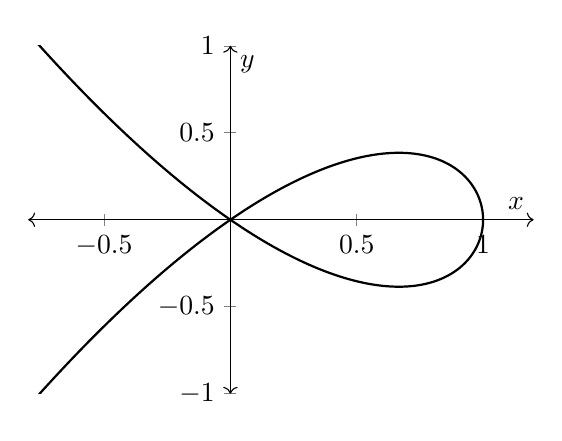
\begin{tikzpicture}
				\begin{axis}[
					height=6cm,
					width=8cm,
					xmin=-.8,xmax=1.2,
					ymin= -1,ymax=1,
					]
					\addplot [domain=-2:2,samples=1000, thick]({1-x^2},{x*(1-x^2)}); 
				\end{axis}
			\end{tikzpicture}
		\end{center}
		Then $M$ is not a $1$-dimensional topological manifold.\\
		\tbf{Hint:} connected components
	\end{ex}
	
	\begin{proof}
		Suppose that $M$ is a $1$-dimensional manifold. Set $p = (0,0)$. Then there exists $(U, \phi) \in X(M)$ such that $p \in U$. Since $\phi(U)$ is open (in $\R$ or $\H$), there exists a $B \subset \phi(U)$ such that $B$ is open (in $\R$ or $\H$), $B$ is connected and $\phi(p) \in B$. Set $V = \phi^{-1}(B)$, $V' = V \setminus \{p\}$ and $B' = B \setminus \{\phi(p)\}$. Then $\phi: V \rightarrow B$ and $\phi': V' \rightarrow B'$ are homeomorphisms. Since $B$ is open (in $\R$ or $\H$) and connected, $B'$ has at most two connected components. Then $V'$ This is a contradiction since $V'$ has four connected components and $B'$ and $V'$ are homeomorphic. 
	\end{proof}
	
	
	
	\begin{ex} \lex{ex:topological_manifolds_introduction:0023} \tbf{Topological Manifold Chart Lemma:} \\
		Let $M$ be a set, $\Gam$ an index set and for each $\al \in \Gam$, $U_{\al} \subset M$ and $\phi_{\al}: U_{\al} \rightarrow \H^n$. Suppose that 
		\begin{itemize}
			\item for each $\al \in \Gam$, $\phi_{\al}(U_{\al}) \in \MT_{\H^n}$ 
			\item for each $\al, \be \in \Gam$, $\phi_{\al}(U_{\al} \cap U_{\be}) \in \MT_{\H^n}$
			\item for each $\al \in \Gam$, $\phi_{\al}: U_{\al} \rightarrow \phi_{\al}(U_{\al})$ is a bijection
			\item for each $\al, \be \in \Gam$, $\phi_{\be}|_{U_{\al} \cap U_{\be}} \circ (\phi_{\al}|_{U_{\al} \cap U_{\be}})^{-1}: \phi_{\al}(U_{\al} \cap U_{\be}) \rightarrow \phi_{\be}(U_{\al} \cap U_{\be})$ is continuous
			\item there exists $\Gam' \subset \Gam$ such that $\Gam'$ is countable and $M \subset \bigcup\limits_{\al \in \Gam'} U_{\al}$
			\item for each $p,q \in M$, there exists $\al \in \Gam$ such that $p,q \in U_{\al}$ or there exist $\al,\be \in \Gam$ such that $p \in U_{\al}$, $q \in U_{\be}$ and $U_{\al} \cap U_{\be} = \varnothing$
		\end{itemize}
		Define 
		\begin{itemize}
			\item $\MB = \{\phi_{\al}^{-1}(V): V \in \MT_{\H^n} \text{ and $\al \in \Gam$} \}$
			\item $\MT_M = \tau(\MB)$
		\end{itemize}
		Then  
		\begin{enumerate}
			\item $\MB$ is a basis for $\MT_M$ \\
			\tbf{Hint:} For $B_1, B_2 \subset \H^n$, $\phi_{\al_1}^{-1}(B_1) \cap \phi_{\al_2}^{-1}(B_2) = \phi_{\al_1}^{-1}( B_1 \cap [\phi_{\al_1}|_{U_{\al_1} \cap U_{\al_2}} \circ (\phi_{\al_2}|_{U_{\al_1} \cap U_{\al_2}})^{-1}(B_2)])$
			\item $(M, \MT_M)$ is an $n$-dimensional topological manifold
			\item $\MT_M$ is the unique topology $\MT$ on $M$ such that $(U_{\al}, \phi_{\al})_{\al \in \Gam} \subset X^n(M, \MT)$
		\end{enumerate}
	\end{ex}
	
	\begin{proof} \
		\begin{enumerate}
			\item \begin{itemize}
				\item By assumption, $M \subset \bigcup\limits_{\al \in \Gam} U_{\al}$
				\item Let $A_1, A_2 \in \MB$ and $p \in A_1 \cap A_2$. By definition, there exist $\al_1, \al_2 \in \Gam$ and $B_1, B_2 \subset \H^n$ such that $B_1$, $B_2$ are open in $\H^n$ and 
				\begin{align*}
					A_1 & = \phi_{\al_1}^{-1}(B_1)  & A_2 & = \phi_{\al_2}^{-1}(B_2) \\
					& \subset U_{\al_1}         &     & \subset U_{\al_2}
				\end{align*}
				Set $\psi_1 = \phi_{\al_1}|_{U_{\al_1} \cap U_{\al_2}}$ and $\psi_2 = \phi_{\al_2}|_{U_{\al_1} \cap U_{\al_2}}$. We note that  
				\begin{align*}
					\psi_1^{-1}(B_1) & = U_{\al_2} \cap \phi_{\al_1}^{-1}(B_1) &  \psi_2^{-1}(B_2) & = U_{\al_1} \cap \phi_{\al_2}^{-1}(B_2) \\
					& = U_{\al_2} \cap A_1                    &                   & = U_{\al_1} \cap A_2 \\
					& \subset U_{\al_1} \cap U_{\al_2}        &                   & \subset U_{\al_1} \cap U_{\al_2}
				\end{align*}
				Let $q \in \phi_{\al_1}^{-1}(B_1 \cap [\psi_1 \circ \psi_2^{-1}(B_2)])$. Then $\phi_{\al_1}(q) \in B_1 \cap [\psi_1 \circ \psi_2^{-1}(B_2)]$. Hence $\phi_{\al_1}(q) \in B_1$ and $\phi_{\al_1}(q) \in \psi_1 \circ \psi_2^{-1}(B_2)$. This implies that  
				\begin{align*}
					q 
					& \in \phi_{\al_1}^{-1}(B_1) \\
					& = A_1
				\end{align*}
				and since $\psi_2^{-1}(B_2) \subset U_{\al_1} \cap U_{\al_2}$ and $\phi_{\al_1}: U_{\al_1} \rightarrow \phi_{\al_1}(U_{\al_1})$ is a bijection, we have that
				\begin{align*}
					q 
					& \in \phi_{\al_1}^{-1}(\psi_1 \circ \psi_2^{-1}(B_2)) \\
					& = \psi_2^{-1}(B_2) \\
					& = U_{\al_1} \cap A_2 
				\end{align*} 
				Thus 
				\begin{align*}
					q 
					& \in A_1 \cap (U_{\al_1} \cap A_2) \\
					& = A_1 \cap A_2
				\end{align*}
				Since $q \in \phi_{\al_1}^{-1}(B_1 \cap [\psi_1 \circ \psi_2^{-1}(B_2)])$ is arbitrary, we have that $\phi_{\al_1}^{-1}(B_1 \cap [\psi_1 \circ \psi_2^{-1}(B_2)]) \subset A_1 \cap A_2$. \\
				Conversely, let  
				\begin{align*}
					q 
					& \in A_1 \cap A_2 \\ 
					& = \phi_{\al_1}^{-1}(B_1) \cap \phi_{\al_2}^{-1}(B_2)
				\end{align*}
				Then $\phi_{\al_1}(q) \in B_1$ and $\phi_{\al_2}(q) \in B_2$. Since $A_1 \cap A_2 \subset U_{\al_1} \cap U_{\al_2}$, we have that 
				\begin{align*}
					\psi_2(q)
					& = \phi_{\al_2}(q) \\
					& \in B_2
				\end{align*}
				which implies that $q \in \psi_2^{-1}(B_2)$. Therefore 
				\begin{align*}
					\phi_{\al_1}(q)
					& = \psi_1(q) \\
					& \in \psi_1 ( \psi_2^{-1}(B_2)) \\
					& =  \psi_1 \circ \psi_2^{-1}(B_2) 
				\end{align*}
				Hence $\phi_{\al_1}(q) \in B_1 \cap [\psi_1 \circ \psi_2^{-1}(B_2)]$. This implies that $q \in \phi_{\al_1}^{-1}( B_1 \cap [\psi_1 \circ \psi_2^{-1}(B_2)])$. Since $q \in A_1 \cap A_2$ is arbitrary, we have that $A_1 \cap A_2 \subset \phi_{\al_1}^{-1}( B_1 \cap [\psi_1 \circ \psi_2^{-1}(B_2)])$. Thus 
				\begin{align*}
					A_1 \cap A_2 
					& = \phi_{\al_1}^{-1}( B_1 \cap [\psi_1 \circ \psi_2^{-1}(B_2)]) \\
					& \in \MB
				\end{align*}
				Thus $\MB$ is a basis for $\MT_M$.
			\end{itemize}
			\item 
			\begin{enumerate}
				\item \tbf{(locally Euclidean of dimension $n$):}\\
				Let $\al \in \Gam$. By definition, for each $B \subset \MT_{\H^n}$, 
				\begin{align*}
					\phi_{\al}^{-1}(B) 
					& \in \MB \\
					& \subset \MT_M
				\end{align*}
				Hence $\phi_{\al}$ is continuous. \\
				Let $A \in \MT_{U_{\al}}$. Then there exists $U \subset \MT_M$ such that $A = U \cap U_{\al}$. Since $\MB$ is a basis for $\MT_M$, there exists $\Gam' \subset \Gam$, $(V_{\be})_{\be \in \Gam'} \subset \MT_{\H^n}$ such that $U = \bigcup_{ \be \in \Gam'} \phi_{\be}^{-1}(V_{\be})$. Thus 
				\begin{align*}
					A
					& = U \cap U_{\al} \\
					& = \bigg[\bigcup_{\be \in \Gam'} \phi_{\be}^{-1}(V_{\be}) \bigg] \cap U_{\al} \\ 
					& = \bigcup_{\be \in \Gam'} [\phi_{\be}^{-1}(V_{\be}) \cap U_{\al}] \\
				\end{align*} 
				Let $\be \in \Gam'$. Since $\phi_{\al}(U_{\al} \cap U_{\be}) \subset \phi_{\al}(U_{\al})$ and $\phi_{\al}(U_{\al} \cap U_{\be}) \in \MT_{\H^n}$, we have that
				\begin{align*}
					\phi_{\al}(U_{\al} \cap U_{\be})
					& = \phi_{\al}(U_{\al}) \cap \phi_{\al}(U_{\al} \cap U_{\be}) \\
					& \in \MT_{\phi_{\al}(U_{\al})}
				\end{align*}
				Therefore $\MT_{\phi_{\al}(U_{\al} \cap U_{\be})} \subset \MT_{\phi_{\al}(U_{\al})}$. Since $(\phi_{\be}|_{U_{\al} \cap U_{\be}}) \circ (\phi_{\al}|_{U_{\al} \cap U_{\be}})^{-1}: \phi_{\al}(U_{\al} \cap U_{\be}) \rightarrow \phi_{\be}(U_{\al} \cap U_{\be})$ is continuous, we have that $(\phi_{\be}|_{U_{\al} \cap U_{\be}}) \circ (\phi_{\al}|_{U_{\al} \cap U_{\be}})^{-1}: \phi_{\al}(U_{\al} \cap U_{\be}) \rightarrow \H^n$
				is continuous and therefore 
				\begin{align*}
					[(\phi_{\be}|_{U_{\al} \cap U_{\be}}) \circ (\phi_{\al}|_{U_{\al} \cap U_{\be}})^{-1}]^{-1}(V_{\be}) 
					& \in \MT_{\phi_{\al}(U_{\al} \cap U_{\be})} \\
					& \subset \MT_{\phi_{\al}(U_{\al})}
				\end{align*} 
				Since $\be \in \Gam'$ is arbitrary, we have that
				\begin{align*}
					\phi_{\al}(A)
					& = \phi_{\al} \bigg( \bigcup_{\be \in \Gam'} [\phi_{\be}^{-1}(V_{\be}) \cap U_{\al}] \bigg) \\
					& = \bigcup_{\be \in \Gam'} \phi_{\al}(\phi_{\be}^{-1}(V_{\be}) \cap U_{\al}) \\
					& =  \bigcup_{\be \in \Gam'} (\phi_{\al}|_{U_{\al} \cap U_{\be}}) \circ (\phi_{\be}|_{U_{\al} \cap U_{\be}})^{-1}(V_{\be}) \\
					& =  \bigcup_{\be \in \Gam'} [(\phi_{\be}|_{U_{\al} \cap U_{\be}}) \circ (\phi_{\al}|_{U_{\al} \cap U_{\be}})^{-1}]^{-1}(V_{\be}) \\
					& \in \MT_{\phi_{\al}(U_{\al})}
				\end{align*} 
				Since $A \in \MT_{U_{\al}}$ is arbitrary, $\phi_{\al}^{-1}: \phi_{\al}(U_{\al}) \rightarrow U_{\al}$ is continuous. Hence $\phi_{\al}: U_{\al} \rightarrow \phi_{\al}(U_{\al})$ is a homeomorphism and $(U_{\al}, \phi_{\al}) \in X^n(M)$. Since $M = \bigcup\limits_{\al \in \Gam} U_{\al}$, we have that $M$ is locally Euclidean of dimension $n$.
				\item \tbf{(Hausdorff):} \\
				Let $p, q \in M$. Suppose that $p \neq q$. Then there exists $\al \in \Gam$ such that $p,q \in U_{\al}$ or there exist $\al, \be \in \Gam$ such that $p \in U_{\al}$, $q \in U_{\be}$ and $U_{\al} \cap U_{\be} = \varnothing$.
				\begin{itemize}
					\item Suppose that there exists $\al \in \Gam$ such that $p,q \in U_{\al}$. Since $p \neq q$, $\phi_{\al}(p) \neq \phi_{\al}(q)$. Since $\H^n$ is Hausdorff, there exist $V_p , V_q \subset \phi(U_{\al})$ such that $V_p$ and $V_q$ are open in $\H^n$, $p \in V_p$, $q \in V_q$ and $V_p \cap V_q = \varnothing$. Set $U_p = \phi_{\al}^{-1}(V_p)$ and $U_q = \phi_{\al}^{-1}V_q$. Then $U_p, U_q$ are open, $p \in U_p$, $q \in U_q$ and $U_q \cap U_p = \varnothing$.
					\item Suppose that there exist $\al, \be \in \Gam$ such that $p \in U_{\al}$, $q \in U_{\be}$ and $U_{\al} \cap U_{\be} = \varnothing$. Set $U_p = U_{\al}$ and $U_q = U_{\be}$. Then $U_p, U_q$ are open, $p \in U_p$, $q \in U_q$ and $U_q \cap U_p = \varnothing$.
				\end{itemize}
				Thus for each $p, q \in M$ there exist $U_p, U_q \subset M$ such that $U_p, U_q$ are open, $p \in U_p$, $q \in U_q$ and $U_q \cap U_p = \varnothing$. Hence 
				\item \tbf{(second-countable):} \\
				By assumption, there exists $\Gam' \subset \Gam$ such that $\Gam'$ is countable and $M \subset \bigcup\limits_{\al \in \Gam'} U_{\al}$. Let $\al \in \Gam'$. Since $\phi_{\al}(U_{\al}) \in \MT_{\H^n}$ and $\H^n$ is second-countable, we have that $\phi_{\al}(U_{\al})$ is second-countable. Since $\phi_{\al}: U_{\al} \rightarrow \phi_{\al}(U_{\al})$ is a homeomorphism, we have that $U_{\al}$ is second-countable. Since $M = \bigcup\limits_{\al \in \Gam'} U_{\al}$, an exercise in topology \tcb{cite} implies that $M$ is second-countable.
			\end{enumerate} 
			\item Let $\MT$ be a topology on $M$. Suppose that $(U_{\al}, \phi_{\al})_{\al \in \Gam} \subset X^n(M, \MT)$. Then for each $\al \in \Gam$, $U_{\al} \in \MT$ and $\phi_{\al}: U_{\al} \rightarrow \phi_{\al}(U_{\al})$ is a $(\MT \cap U_{\al}, \MT_{\H^n} \cap \phi_{\al}(U_{\al}))$-homeomorphism. \\ 
			Let $U \in \MB$. By definition, there exists $\al \in \Gam$ and $V \in \MT_{\H^n}$ such that $U = \phi_{\al}^{-1}(V)$. Since $U_{\al} \in \MT$, we have that $\MT \cap U_{\al} \subset \MT$. Since $V \cap \phi_{\al}(U_{\al}) \in \MT_{\H^n} \cap \phi_{\al}(U_{\al})$, and $\phi_{\al}$ is a  $(\MT \cap U_{\al}, \MT_{\H^n} \cap \phi_{\al}(U_{\al}))$-homeomorphism, we have that
			\begin{align*}
				U
				& = \phi_{\al}^{-1}(V) \\
				& = \phi_{\al}^{-1}(V \cap \phi_{\al}(U_{\al})) \\
				& \in \MT \cap U_{\al} \\
				& \subset \MT 
			\end{align*}
			Since $U \in \MB$ is arbitrary, $\MB \subset \MT$. Therefore 
			\begin{align*}
				\MT_M 
				& = \tau(\MB) \\
				& \subset \tau(\MT) \\
				& = \MT
			\end{align*}
			Conversely, Let $U \in \MT$ and $\al \in \Gam$. Then $U \cap U_{\al} \in \MT \cap U_{\al}$. Since $\phi_{\al}:U_{\al} \rightarrow \phi_{\al}(U_{\al})$ is a $(\MT \cap U_{\al}, \MT_{\H^n} \cap \phi_{\al}(U_{\al}))$-homeomorphism, we have that $\phi_{\al}(U \cap U_{\al}) \in \MT_{\H^n} \cap \phi_{\al}(U_{\al})$. Since $U_{\al} \in \MT_M$, $\MT_M \cap U_{\al} \subset \MT_M$. Since $\phi_{\al}:U_{\al} \rightarrow \phi_{\al}(U_{\al})$ is a $(\MT_M \cap U_{\al}, \MT_{\H^n} \cap \phi_{\al}(U_{\al}))$-homeomorphism, we have that 
			\begin{align*}
				U \cap U_{\al}
				& = \phi_{\al}^{-1}( \phi_{\al}(U \cap U_{\al})) \\
				& \in \MT_M \cap U_{\al} \\
				& \subset \MT_M 
			\end{align*}
			Then 
			\begin{align*}
				U
				& = U \cap M \\
				& = U \cap \bigg(\bigcup_{\al \in \Gam} U_{\al} \bigg) \\
				& = \bigcup_{\al \in \Gam} (U \cap U_{\al}) \\
				& \in \MT_M 
			\end{align*}
			Since $U \in \MT$ is arbitrary, $\MT \subset \MT_M$. Thus $\MT = \MT_M$.
		\end{enumerate}
	\end{proof}
	
	\begin{ex} \lex{ex:topological_manifolds_introduction:0024}
		Let $M$ be a set, $\Gam$ an index set and for each $\al \in \Gam$, $U_{\al} \subset M$ and $\phi_{\al}: U_{\al} \rightarrow \H^n$. Suppose that 
		\begin{itemize}
			\item for each $\al \in \Gam$, $\phi_{\al}(U_{\al}) \in \MT_{\H^n}$ 
			\item for each $\al, \be \in \Gam$, $\phi_{\al}(U_{\al} \cap U_{\be}) \in \MT_{\H^n}$
			\item for each $\al \in \Gam$, $\phi_{\al}: U_{\al} \rightarrow \phi_{\al}(U_{\al})$ is a bijection
			\item for each $\al, \be \in \Gam$, $\phi_{\be}|_{U_{\al} \cap U_{\be}} \circ (\phi_{\al}|_{U_{\al} \cap U_{\be}})^{-1}: \phi_{\al}(U_{\al} \cap U_{\be}) \rightarrow \phi_{\be}(U_{\al} \cap U_{\be})$ is continuous
			\item there exists $\Gam' \subset \Gam$ such that $\Gam'$ is countable and $M \subset \bigcup\limits_{\al \in \Gam'} U_{\al}$
			\item for each $p,q \in M$, there exists $\al \in \Gam$ such that $p,q \in U_{\al}$ or there exist $\al,\be \in \Gam$ such that $p \in U_{\al}$, $q \in U_{\be}$ and $U_{\al} \cap U_{\be} = \varnothing$
		\end{itemize}
		Then there exists a unique topology $\MT_M$ on $M$ such that $(M, \MT_M)$ is an $n$-dimensional topological manifold and $(U_{\al}, \phi_{\al})_{\al \in \Gam} \subset X^n(M, \MT_M)$.
	\end{ex}
	
	\begin{proof}
		Immediate by previous exercise. 
	\end{proof}
	

























	\newpage
	\section{Submanifolds}
	
	\subsection{Open Submanifolds}
	
	\begin{note} 
		Let $(M, \MT)$ be an $n$-dimensional topological manifold and $U \subset M$. Suppose that $U$ is open in $M$. Unless otherwise specified, we equip $U$ with $\MT \cap U$. 
	\end{note}

	\begin{ex} \lex{ex:topological_open_submanifolds:0001}
		Let $M$ be an $n$-dimensional topological manifold, $(U, \phi) \in X(M)$ and $U' \subset U$. If $U'$ is open in $M$, then $(U', \phi|_{U'}) \in X^n(M)$. 
	\end{ex}
	
	\begin{proof}
		Suppose that $U'$ is open in $M$. Set $\phi' = \phi|_{U'}$. 
		\begin{itemize}
			\item By assumption $U'$ is open in $M$.
			\item Since $U'$ is open in $M$, we have that $U' = U' \cap U$ is open in $U$. Since $\phi$ is a homeomorphism and $U'$ is open in $U$, we have that $\phi(U')$ is open in $\phi(U)$. By assumption $\phi(U)$ is open in $\R^n$ or $\phi(U)$ is open in $\H^n$. Therefore $\phi'(U')$ is open in $\R^n$ or $\phi'(U')$ is open in $\H^n$.
			\item Since $\phi:U \rightarrow V$ is a homeomorphism, $\phi': U' \rightarrow \phi'(U')$ is a homeomorphism. 
		\end{itemize}
		So $(U', \phi') \in X^n(M)$. 
	\end{proof}
	
	\begin{note}
		Since $U$ is open in $M$, $U'$ being open in $U$ is equivalent to $U'$ being open in $M$, so we could have also assumed that $U'$ is open in $U$.
	\end{note}
	
	\begin{ex} \lex{ex:topological_open_submanifolds:0002}
		Let $M$ be an $n$-dimensional topological manifold and $U \subset M$. If $U$ is open, then 
		$$X^n(U) = \{(V, \psi) \in X^n(M): V \subset U\}$$
	\end{ex}
	
	\begin{proof}
		Suppose that $U$ is open and set $A = \{(V, \psi) \in X^n(M): V \subset U\}$. Let $(V, \psi) \in X^n(U)$. By definition of $X^n(U)$, $V$ is open in $U$. Thus, there exists $W \subset M$ such that $W$ is open in $M$ and $V = U \cap W$. Since $U$ is open in $M$, we have that $V = U \cap W$ is open in $M$. Hence $(V, \psi) \in X^n(M)$ which implies that $(V, \psi) \in A$. Since $(V, \psi) \in X^n(U)$ is arbitary, $X^n(U) \subset A$. \\
		Conversely, suppose that $(V, \psi) \in A$. Then $(V, \psi) \in X^n(M)$ and $V \subset U$. By definition of $X^n(M)$, $V$ is open in $M$. Since $V \subset U$, we have that $V = V \cap U$ is open in $U$. Hence $(V, \psi) \in X^n(U)$. Since $(V, \psi) \in X^n(U)$ is arbitary, $A \subset X^n(U)$. Hence $X^n(A) = A$.
	\end{proof}
	
	\begin{ex} \lex{ex:topological_open_submanifolds:0003}
		Let $M$ be an $n$-dimensional topological manifold, $(U, \phi) \in X(M)$ and $U' \subset U$. If $U'$ is open in $M$, then $(U', \phi|_{U'}) \in X^n(U)$. 
	\end{ex}
	
	\begin{proof}
		Suppose that $U'$ is open in $M$. A previous exercise implies that $(U', \phi') \in X^n(M)$. The previous exercise implies that $(U', \phi') \in X^n(U)$.
	\end{proof}
	
	\begin{ex} \lex{ex:topological_open_submanifolds:0004} \tbf{Topological Open Submanifolds:}\\
		Let $M$ be an $n$-dimensional topological manifold and $U \subset M$ open. Then $U$ is an $n$-dimensional topological manifold. 
	\end{ex}
	
	\begin{proof} \
		\begin{enumerate}
			\item Since $M$ is Hausdorff, $U$ is Hausdorff.
			\item Since $M$ is second-countable, $U$ is second countable. 
			\item Let $p \in U$. Since then there exists $(V, \psi) \in X^n(M)$ such that $p \in V$. Set $V' = U \cap V$ and $\psi' = \psi|_{U \cap V}$. The previous exercise implies that $(V', \psi') \in X^n(U)$. Therefore $U$ is locally Euclidean of dimension $n$.
		\end{enumerate}
		Hence $U$ is an $n$-dimensional topological manifold.
	\end{proof}

	\begin{ex} \lex{ex:topological_open_submanifolds:0005}
		Let $M$ be an $n$-dimensional topological manifold and $U \subset M$. If $U$ is open, then 
		\begin{enumerate}
			\item $X_{\Int}(U) = \{(V, \psi) \in X_{\Int}(M): V \subset U\}$
			\item $X_{\p}(U) = \{(V, \psi) \in X_{\p}(M): V \subset U\}$
		\end{enumerate}
	\end{ex}
	
	\begin{proof}
		Suppose that $U$ is open in $M$.
		\begin{enumerate}
			\item Set $A = \{(V, \psi) \in X_{\Int}(M): V \subset U\}$. Let $(V, \psi) \in X_{\Int}(U)$. By definition of $X_{\Int}(U)$, $V$ is open in $U$ and $\phi(V)$ is open in $\R^n$. Since $U$ is open in $M$, $V$ is open in $M$. Hence $(V, \psi) \in X_{\Int}(M)$. Since $U$ is open in $M$, $V$ is open in $M$. Hence $(V, \psi) \in X_{\Int}(M)$ which implies that $(V, \psi) \in A$. Since $(V, \psi) \in X_{\Int}(U)$ is arbitrary, $X_{\Int}(U) \subset A$. \\
			Conversely, let $(V, \psi) \in A$. Then $(V, \psi) \in X_{\Int}(M)$ and $V \subset U$. By definition of $X_{\Int}(M)$, $V$ is open in $M$ and $\phi(V)$ is open in $\R^n$. Thus $V = V \cap U$ is open in $U$. So $(V, \psi) \in X_{\Int}(U)$. Since $(V, \psi) \in A$ is arbitrary, $A \subset X_{\Int}(U)$. Thus $X_{\Int}(U) = A$.
			
			\item Set $B = \{(V, \psi) \in X_{\p}(M): V \subset U\}$. Let $(V, \psi) \in X_{\p}(U)$. By definition of $X_{\p}(U)$, $V$ is open in $U$, $\phi(V)$ is open in $\H^n$ and $\p \H^n_j \cap \phi(V) \neq \varnothing$. Since $U$ is open in $M$, $V$ is open in $M$. Hence $(V, \psi) \in X_{\p}(M)$, which implies that $(V, \psi) \in B$. Since $(V, \psi) \in X_{\p}(U)$ is arbitrary, $X_{\p}(U) \subset B$. \\
			Conversely, let $(V, \psi) \in B$. Then $(V, \psi) \in X_{\p}(M)$ and $V \subset U$. By definition of $X_{\p}(M)$, $V$ is open in $M$, $\phi(V)$ is open in $\H^n$ and $\p \H^n_j \cap \phi(V) \neq \varnothing$. Thus $V = V \cap U$ is open in $U$. So $(V, \psi) \in X_{\p}(U)$. Since $(V, \psi) \in B$ is arbitrary, $B \subset X_{\p}(U)$. Thus $X_{\p}(U) = B$.
		\end{enumerate}
	\end{proof}
	

	\begin{ex} \lex{ex:topological_open_submanifolds:0006}
		Let $M$ be an $n$-dimensional topological manifold and $U \subset M$. If $U$ is open, then $\p U = \p M \cap U$.
	\end{ex}

	\begin{proof}
		Suppose that $U$ is open. Let $p \in \p U$. Then there exists $(V, \psi) \in X_{\p}(U)$ such that $p \in V$ and $\psi(p) \in \p \H^n$. Since $U$ is open, the previous exercise implies that $(V, \psi) \in X_{\p}(M)$. Thus $p \in \p M$. Since $p \in \p U$ is arbitrary, $\p U \subset \p M$. Since $\p U \subset U$, we have that $\p U \subset \p M \cap U$.\\
		Conversely, let $p \in \p M \cap U$. Since $p \in \p M$, there exists $(V, \psi) \in X_{\p}(M)$ such that $p \in V$ and $\psi(p) \in \p \H^n$. Set $V' = V \cap U$ and $\psi' = \psi|_{V'}$. Then $p \in V'$ since $V$ and $U$ are open in $M$, $V'$ is open in $M$. A previous exercise implies that $(V', \psi') \in X(M)$. Since $p \in \p M$, a previous exercise implies that $(V', \psi') \in X_{\p}(M)$. The previous exercise implies that $(V', \psi') \in X_{\p}(U)$. Since $\psi'(p) \in \p \H^n$, $p \in \p U$. Since $p \in \p M \cap U$ is arbitrary, $\p M \cap U \subset \p U$. Hence  $\p U = \p M \cap U$. \\
		\tcb{label exercises and reference them!!!}
	\end{proof}




















\subsection{Boundary Submanifolds}

\begin{note} 
	Let $(M, \MT)$ be an $n$-dimensional topological manifold. Unless otherwise specified, we equip $\p M$ with $\MT \cap \p M$. 
\end{note}

\begin{defn}
	Let $M$ be an $n$-dimensional topological manifold and $\pi:\p \H^n_j \rightarrow \R^{n-1}$ the projection map. For $(U, \phi) \in X_{\p}(M)$, we define $\bar{U} \subset \p M$ and $\bar{\phi}: \bar{U} \rightarrow \pi (\phi(\bar{U}))$ by $\bar{U} = U \cap \p M$ and $\bar{\phi} = \pi \circ \phi|_{\bar{U}}$ respectively. 
\end{defn}

\begin{ex}
	Let $M$ be an $n$-dimensional topological manifold,  and $\lam: \p \H^n_j \rightarrow \R^{n-1}$ a homeomorphism. Then $\{(\bar{U}, \bar{\phi}): (U, \phi) \in X_{\p}(M)\} \subset X^{n-1}_{\Int}(\p M)$.
\end{ex}

\begin{proof}
	Let $(U, \phi) \in X_{\p}(M)$.
	\begin{enumerate}
		\item Since $U$ is open in $M$, $\bar{U} = U \cap \p M$ is open in $\p M$. 
		\item Since $(U, \phi) \in X_{\p}(M)$, $\phi(U)$ is open in $\H^n$. A previous exercise implies that $\phi(\bar{U}) = \phi(U) \cap \p \H^n$ which is open in $\p \H^n$. Since $\pi: \p \H^n_j \rightarrow \R^{n-1}$ is a homeomorphism, we have that $\pi(\phi(\bar{U}))$ is open in $\R^{n-1}$. 
		\item Since $\phi|_{\bar{U}}: \bar{U} \rightarrow \phi(U) \cap \p \H^n$ and $\pi|_{\phi(\bar{U})} : \phi(\bar{U}) \rightarrow \lam(\phi(\bar{U})) $ are homeomorphisms, we have that $\bar{\phi} = \pi|_{\phi(\bar{U})} \circ \phi|_{\bar{U}}$ is a homeomorphism.
	\end{enumerate}
	Hence $(\bar{U}, \bar{\phi}) \in  X^{n-1}_{\Int}(\p M)$.
\end{proof}

\begin{ex} \tbf{Topological Boundary Submanifold:} \\
	Let $M$ be an $n$-dimensional topological manifold. Then 
	\begin{enumerate}
		\item $\p M$ is an $(n-1)$-dimensional topological manifold
		\item $\p (\p M) = \varnothing$
	\end{enumerate}
\end{ex}

\begin{proof}\
	\begin{enumerate}
		\item 
		\begin{enumerate}
			\item Since $M$ is Hausdorff, $\p M$ is Hausdorff.
			\item Since $M$ is second-countable, $\p M$ is second countable. 
			\item Let $p \in \p M$. Then there exists $(U, \phi) \in X_{\p}(M)$ such that $\phi(p) \in \p \H^n$. Then $p \in \bar{U}$ and the previous exercise implies that $(\bar{U}, \bar{\phi}) \in X^{n-1}_{\Int}(\p M)$. Thus $\p M$ is locally Euclidean of dimension $n-1$.
		\end{enumerate}
		Hence $\p M$ is an $(n-1)$-dimensional topological manifold.
		\item Let $p \in \p M$. Part $(1)$ implies that there exists $(U, \phi) \in X^{n-1}_{\Int}(\p M)$ such that $p \in U$. Thus $p \in \Int \p M$. Since $p \in \p M$ is arbitrary, $\Int \p M = \p M$. Hence 
		\begin{align*}
			\p (\p M)
			& = (\Int(\p M))^c \\
			& = (\p M)^c \\
			& = \varnothing
		\end{align*} 
	\end{enumerate}
\end{proof}








































\subsection{Embedded Submanifolds}

\begin{ex} \lex{ex:top_submanifolds:embedded:0001}
	Let $M, N \in \Obj(\Man0)$ and $F \in \Hom_{\Top}(N, M)$. Define 
	$$F_*X^n(N, \MT_N) \defeq \{(F(V), \psi \circ F|_V^{-1}): (V, \psi) \in X^n(N, \MT_N)\}.$$ 
	If $F$ is a $\Top$-embedding, then 
	\begin{enumerate}
		\item $F_*X^n(N, \MT_N) \subset X^n(F(N), \MT_M \cap F(N))$.
		\item $(F(N), \MT_M \cap F(N)) \in \Obj(\Man0)$.
	\end{enumerate}
\end{ex}

\begin{proof}
	Suppose that $F$ is a $\Top$-embedding. Set $n \defeq \dim N$. Since $F$ is a $\Top$-embedding, $F \in \Iso_{\Top}((N, \MT_N), (F(N), \MT_M \cap F(N)))$.
	\begin{enumerate}
		\item Let $(U, \phi) \in F_*X^n(N, \MT_N)$. Then there exists $(V, \psi) \in \MA_N$ such that $U = F(V)$ and $\phi = \psi \circ F|_V^{-1}$. Since $(V, \psi) \in \MA_N$ and $\MA_N \subset X^n(N, \MT_N)$, we have that $(V, \psi)$ is an $\R^n$-coordinate chart on $(N, \MT_N)$ or there exists $j \in [n]$ such that $(V, \psi)$ is an $\H^n_j$-coordinate chart on $(N, \MT_N)$. 
		\begin{itemize}
			\item Suppose that $(V, \psi)$ is an $\R^n$-coordinate chart on $(N, \MT_N)$. 
			\begin{itemize}
				\item Since $V \in \MT_N$, we have that 
				\begin{align*}
					U
					& = F(V) \\
					& \in \MT_M \cap F(N).
				\end{align*}
				\item Since $F \in \Iso_{\Top}((N, \MT_N), (F(N), \MT_M \cap F(N)))$, we have that 
				\begin{align*}
					F|_V 
					& \in \Iso_{\Top}((V, \MT_N \cap V), (F(V), [\MT_M \cap F(N)] \cap F(V))) \\
					& = \Iso_{\Top}((V, \MT_N \cap V), (F(V), \MT_M \cap F(V))).
				\end{align*}
				Since $(V, \psi)$ is an $\R^n$-coordinate chart on $(N, \MT_N)$, we have that $\psi(V) \in \MT_{\R^n}$. Thus 
				\begin{align*}
					\phi(U)
					& = \psi \circ F|_V^{-1}( F(V)) \\
					& = \psi(V) \\
					& \in \MT_{\R^n}.
				\end{align*}
				\item Since $\psi \in \Iso_{\Top}((V, \MT_N \cap V), (\psi(V), \MT_{\R^n} \cap \psi(V))$, and $F|_V^{-1} \in \Iso_{\Top}((F(V), \MT_M \cap F(V)), (V, \MT_N \cap V))$, we have that $\psi \circ F|V^{-1} \in \Iso_{\Top}((F(V), \MT_M \cap F(V)), (\psi(V), \MT_{\R^n} \cap \psi(V))$. 
			\end{itemize}
			Hence $(U, \phi) \in X^n(F(N), \MT_M \cap F(N))$.
			\item Similarly, if there exists $j \in [n]$ such that $(V, \psi)$ is an $\H^n_j$-coordinate chart on $(N, \MT_N)$, then $(U, \phi) \in X^n(F(N), \MT_M \cap F(N))$.
		\end{itemize}
		Since $(U, \phi) \in F_*X^n(N, \MT_N)$ is arbitrary, we have that $F_*X^n(N, \MT_N) \subset X^n(F(N), \MT_M \cap F(N))$.
		\item 
		\begin{enumerate}
			\item Since $F \in \Iso_{\Top}((N, \MT_N), (F(N), \MT_M \cap F(N)))$ and $(N, \MT_N)$ is Hausdorff, $(F(N), \MT_M \cap F(N))$ is Hausdorff.
			\item Since $F \in \Iso_{\Top}((N, \MT_N), (F(N), \MT_M \cap F(N)))$ and $(N, \MT_N)$ is second-countable, $(F(N), \MT_M \cap F(N))$ is second-countable.
			\item Let $p \in F(N)$. Then there exists $q \in N$ such that $F(q) = p$. Since $N \in \Obj(\Man0)$, there exists $(V, \psi) \in X^n(N, \MT_N)$ such that $q \in V$. Define $(U, \phi) \in F_*X^n(N, \MT_N)$ by $U \defeq F(V)$ and $\phi \defeq \psi \circ F|_V^{-1}$. By definition, $(U, \phi) \in F_*X^n(N, \MT_N)$. Furthermore,  
			\begin{align*}
				p
				& = F(q) \\
				& \in F(V) \\
				& = U.
			\end{align*}
			Since $p \in F(N)$ is arbitrary, we have that for each $p \in F(N)$, there exists $(U, \phi) \in F_*X^n(N, \MT_N)$ such that $p \in U$. Hence $(F(N), \MT_M \cap F(N))$ is locally Euclidean of dimension $n$. 
		\end{enumerate}
		Thus $(F(N), \MT_M \cap F(N)) \in \Obj(\Man0)$. 
	\end{enumerate}
\end{proof}

























\newpage
\section{Product Manifolds}

\begin{note} 
	Let $(M, \MT_M)$ and $(N, \MT_N)$ be $m$-dimensional and $n$-dimensional topological manifold respectively. Unless otherwise specified, we equip $M \times N$ with $\MT_M \otimes \MT_N$. 
\end{note}

\begin{defn} \ld{def:topological_product_manifolds:0002}
	Let $m \in \N$ and $n \in \N_0$. Define $\lam_0: \H^m_j \times \Int \H^n_j \rightarrow \H^{m+n}$ by $\lam((x^1, \ldots, x^{m-1}, x^m), (y^1, \ldots, y^n)) \defeq (x^1, \ldots, x^{m-1}, y^1, \ldots, y^{n-1}, \log y^n, x^m)$.  
\end{defn}

\begin{ex} \lex{ex:topological_product_manifolds:0003}
	Let $m \in \N$ and $n \in \N_0$. Then 
	\begin{enumerate}
		\item $\lam_0$ is a $(\MT_{\H^m} \otimes \MT_{\Int \H^n}, \MT_{\H^{m+n}})$-homeomorphism,
		\item $\lam_0(\p \H^m \times \Int \H^n) = \p \H^{m+n}$,
		\item $(\H^m \times \Int \H^n, \lam_0) \in X^{m+n}(\H^m \times \Int \H^n, \MT_{\H^n} \otimes \MT_{\Int \H^n})$.
	\end{enumerate}
\end{ex}

\begin{proof}\
	\begin{enumerate}
		\item Clearly $\lam_0$ is a homeomorphism.
		\item Clearly $\lam_0(\p \H^m \times \Int \H^n) = \p \H^{m+n}$
		\item We note that
		\begin{itemize}
			\item $\H^m \times \Int \H^n \in \MT_{\H^n} \otimes \MT_{\Int \H^n}$,
			\item $\H^{m+n} \in \MT_{\H^{m+n}}$,
			\item part $(1)$ implies that $\lam_0$ is a $(\MT_{\H^m} \otimes \MT_{\Int \H^n}, \MT_{\H^{m+n}})$-homeomorphism.
		\end{itemize}
		Thus $(\H^m \times \Int \H^n, \lam_0) \in X^{m+n}(\H^m \times \H^n, \MT_{\H^n} \otimes \MT_{\Int \H^n})$.
	\end{enumerate}
\end{proof}

\begin{ex} \lex{ex:topological_product_manifolds:0003.1}
	Let $m, n \in \N_0$. Then $\H^m \times \Int \H^n$ is an $m+n$-dimensional topological manifold.
\end{ex}

\begin{proof} \
	\begin{enumerate}
		\item Clearly $\H^m \times \Int \H^n$ is Hausdorff.
		\item Clearly $\H^m \times \Int \H^n$ is second-countable.
		\item Since $\lam_0 \in X^{m+n}(\H^m \times \H^n, \MT_{\H^n} \otimes \MT_{\Int \H^n})$ , we have that for each $p \in \H^m \times \Int \H^n$, there exists $(U, \phi) \in X^{m+n}(\H^m \times \Int \H^n, \MT_{\H^n} \otimes \MT_{\Int \H^n})$ such that $p \in U$. Thus $(\H^m \times \H^n, \MT_{\H^n} \otimes \MT_{\Int \H^n})$ is locally Euclidean of dimension $m+n$.
	\end{enumerate}
	Thus $(\H^m \times \H^n, \MT_{\H^n} \otimes \MT_{\Int \H^n})$ is an $m+n$-dimensional topological manifold.
\end{proof}


\begin{ex} \lex{ex:topological_product_manifolds:0004}
	Let $(M, \MT_M)$, $(N, \MT_N)$ be topological manifolds. Set $m = \dim M$ and $n = \dim N$. Suppose that $\p N = \varnothing$. Then for each $(U, \phi) \in X^m(M, \MT_M)$, $(V, \psi) \in X^n(N, \MT_N)$, 
	$$(U \times V, \lam_0|_{\phi(U) \times \psi(V)} \circ [\phi \times \psi]) \in X^{m+n}(M \times N, \MT_M \otimes \MT_N)$$ 
\end{ex}

\begin{proof}
	Let $(U, \phi) \in X^m(M, \MT_M)$ and $(V, \psi) \in X^n(N, \MT_N)$. 
	\begin{itemize}
		\item Since $U \in \MT_M$ and $V \in \MT_N$, $U \times V \in \MT_M \otimes \MT_N$. 
		\item Since $\phi(U) \in \MT_{\H^m}$ and $\psi(V) \in \MT_{\H^n}$, $\phi(U) \times \psi(V) \in \MT_{\H^m} \otimes \MT_{\H^n}$. Since $\p N = \varnothing$, $(V, \psi) \in X^n_{\Int}(N, \MT_N)$ and therefore $\psi(V) \subset \Int \H^n$. Since $\lam_0: \H^m \times \Int \H^n \rightarrow \H^{m+n}$ is a homeomorphism, 
		\begin{align*}
			\lam_0|_{\phi(U) \times \psi(V)} \circ [\phi \times \psi](U \times V)
			& = \lam_0 (\phi(U) \times \psi(V)) \\
			& \in \MT_{\H^{m+n}}
		\end{align*}
		\item Since $\phi:U \rightarrow \phi(U)$ is a $(\MT_M \cap U, \MT_{\H^m} \cap \phi(U))$-homeomorphism and $\psi: V \rightarrow \psi(V)$ is a $(\MT_N \cap V, \MT_{\H^n} \cap \psi(V))$-homeomorphism, \tcb{an exercise in the section on product topologies in the analysis notes} implies that $\phi \times \psi: U \times V \rightarrow \phi(U) \times \phi(V)$ is a $([\MT_M \otimes \MT_N] \cap [U \times V], [\MT_{\H^m} \otimes \MT_{\H^n}] \cap [\phi(U) \times \psi(V)])$-homeomorphism. Since $\lam_0|_{\phi(U) \times \psi(V)}: \phi(U) \times \psi(V) \rightarrow \lam_0(\phi(U) \times \psi(V))$ is a $([\MT_{\H^m} \otimes \MT_{\Int \H^n}] \cap[ \phi(U) \times \psi(V)], \MT_{\H^{m+n}} \cap \lam_0(\phi(U) \times \psi(V)))$-homeomorphism, $\lam_0|_{\phi(U) \times \psi(V)} \circ (\phi \times \psi)$ is a $([\MT_M \otimes \MT_N] \cap [U \times V], \MT_{\H^{m+n}} \cap \lam_0(U \times V))$-homeomorphism.
	\end{itemize}
	Hence $(U \times V,\lam_0|_{\phi(U) \times \psi(V)} \circ [\phi \times \psi]) \in X^{m+n}(M \times N, \MT_M \otimes \MT_N)$. Since $(U, \phi) \in X^m(M, \MT_M)$ and $(V, \psi) \in X^n(N, \MT_N)$ are arbitrary, we have that for each $(U, \phi) \in X^m(M, \MT_M)$ and $(V, \psi) \in X^n(N, \MT_N)$, $$(U \times V, \lam_0|_{\phi(U) \times \psi(V)} \circ [\phi \times \psi]) \in X^{m+n}(M \times N,  \MT_M \otimes \MT_N)$$ 
\end{proof}

\begin{ex} \lex{ex:topological_product_manifolds:0005}
	Let $M$, $N$ be topological manifolds. Set $m = \dim M$ and $n = \dim N$. Suppose that $\p N = \varnothing$. Then for each $(U, \phi) \in X^m_{\p}(M, \MT_M)$, $(V, \psi) \in X^n(N, \MT_N)$, 
	$$(U \times V, \lam_0|_{\phi(U) \times \psi(V)} \circ [\phi \times \psi]) \in X^{m+n}_{\p}(M \times N,  \MT_M \otimes \MT_N)$$ 
\end{ex}

\begin{proof}
	Let $(U, \phi) \in X^m_{\p}(M)$ and $(V, \psi) \in X^n(N)$. Define $\eta: U \times V \rightarrow \lam_0(\phi(U) \times \psi(V))$ by 
	$$\eta \defeq \lam_0|_{\phi(U) \times \psi(V)} \circ [\phi \times \psi]$$ 
	Since $(U, \phi) \in X^m_{\p}(M)$, $\phi(U) \cap \p \H^m \neq \varnothing$. Then there exists $p \in U$ such that $\phi(p) \in \p \H^m$. So $\eta(p,q) \in \p \H^{m+n}$. Thus $\eta(U \times V) \cap \p \H^{m+n} \neq \varnothing$ and $(U \times V, \eta) \in X^{m+n}_{\p}(M \times N)$. Since $(U, \phi) \in X^m_{\p}(M)$ and $(V, \psi) \in X^n(N, \MT_N)$ are arbitrary, we have that for each $(U, \phi) \in X^m_p(M, \MT_M)$ and $(V, \psi) \in X^n(N, \MT_N)$, 
	$$(U \times V, \lam_0|_{\phi(U) \times \psi(V)} \circ [\phi \times \psi]) \in X^{m+n}_{\p}(M \times N,  \MT_M \otimes \MT_N)$$ 
\end{proof}

\begin{note}
	The above is still true if $\p N \neq \varnothing$
\end{note}

\begin{ex} \lex{ex:topological_product_manifolds:0006}
	Let $M,N$ be topological manifolds. Suppose that $\p N = \varnothing$. Then 
	\begin{enumerate}
		\item $M \times N$ is a topological manifold
		\item $\p(M \times N) = \p M \times N$
	\end{enumerate}
\end{ex}

\begin{proof}
	 Set $m = \dim M$ and $n = \dim N$. 
	 \begin{enumerate}
	 	\item 
	 	\begin{itemize}
	 		\item Since $M$ and $N$ are Hausdorff, $M \times N$ is Hausdorff.
	 		\item Since $M$ and $N$ are second-countable, $M \times N$ is second-countable.
	 		\item Let $a \in M \times N$. Then there exist $p \in M$ and $q \in N$ such that $a = (p,q)$. Since $M$ and and $N$ are locally Euclidean, there exist $(U, \phi) \in X^m(M)$ and $(V, \psi) \in X^n(N)$ such that $p \in U$ and $q \in V$. Then $(p,q) \in U \times V$. \rex{ex:topological_product_manifolds:0004} implies that $(U \times V, \lam_0 \circ [\phi \times \psi]) \in X^{m+n}(M \times N)$. Since $a \in M \times N$ is arbitrary, $M \times N$ is locally Euclidean of dimension $m+n$.   
	 	\end{itemize}
 		Thus $M \times N$ is an $(m+n)$-dimensional topological manifold.
	 	\item 
	 	\begin{itemize}
	 		\item Let $a \in \p(M \times N)$. Then there exists $p \in M$ and $q \in N$ such that $a = (p,q)$. Since $(M, \MT_M)$ and and $(N)$ are locally Euclidean, there exist $(U, \phi) \in X^m(M)$ and $(V, \psi) \in X^n(N)$ such that $p \in U$ and $q \in V$. Define $\eta: U \times V \rightarrow \lam_0(\phi(U) \times \psi(V))$ by 
	 		$$\eta \defeq \lam_0|_{\phi(U) \times \psi(V)} \circ [\phi \times \psi]$$ 
	 		\rex{ex:topological_product_manifolds:0004} implies that $\eta \in X^{m+n}(M \times N)$. Since $(p, q) \in \p (M \times N)$, \rex{ex:topological_product_manifolds:0005} implies that $\eta \in X^{m+n}_{\p}(M \times N)$ and $\eta(p,q) \in \p \H^{m+n}$. Therefore 
	 		\begin{align*}
	 			\phi \times \psi(p,q)
	 			& = \lam_0|_{\phi(U) \times \psi(V)}^{-1} \circ \eta \\
	 			& \in \p \H^m \times \Int \H^n 
	 		\end{align*}
	 		Hence $\phi(p) \in \p \H^m$ and $\psi(q) \in \Int \H^n$. Thus $(U, \phi) \in X^m_{\p}(M)$ and $p \in \p M$. Therefore  
	 		\begin{align*}
	 			a
	 			& = (p,q) \\
	 			& \in \p M \times N
	 		\end{align*}
	 		Since $a \in \p(M \times N)$ is arbitrary, we have that $\p(M \times N) \subset \p M \times N$.
	 		\item Let $a \in \p M \times N$. Then there exists $p \in \p M$ and $q \in N$ such that $a = (p,q)$. By definition, there exists $(U, \phi) \in X^m_{\p}(M)$ and $(V, \psi) \in X^n(N)$ such that $p \in U$, $q \in V$ and $\phi(p) \in \p \H^m$. Since $\p N = \varnothing$, $\psi(q) \in \Int \H^n$. Define $\eta: U \times V \rightarrow \lam_0(\phi(U) \times \psi(V))$ by 
	 		$$\eta \defeq \lam_0|_{\phi(U) \times \psi(V)} \circ [\phi \times \psi]$$ 
	 		\rex{ex:topological_product_manifolds:0004} implies that $(U \times V, \eta) \in X^{m+n}(M \times N , \MT_M \otimes \MT_N)$. Then
	 		\begin{align*}
	 			\eta(a)
	 			& = \eta(p,q) \\
	 			& = \lam_0(\phi(p), \psi(q)) \\
	 			& \in \p \H^{m+n}
	 		\end{align*} 
	 		Thus $\eta \in X^{m+n}_{\p}(M \times N)$ and $a \in \p (M \times N)$. Since $a \in \p M \times N$ is arbitrary, $\p M \times N \subset \p (M \times N)$. 
	 	\end{itemize}
 		Thus $\p (M \times N) = \p M \times N$. 
	 \end{enumerate}
\end{proof}















































\newpage
\section{Submanifolds}

\begin{defn}
	\tcr{topological embedding}
\end{defn}

\begin{defn}
	Let $M, N$ be topological manifolds of dimensions $m, n$ respectively and $F:N \rightarrow N$ a topological embedding. Then $\{(F(V), \psi \circ F^{-1}): (V, \psi) \in X^n(N)\} \subset X^n(F(N))$. 
\end{defn}

\begin{proof}
	Since 
\end{proof}





























	
	
	
	
	
	
	
	
	
	
	
	
	
	
	
	
	
	
	
	\newpage
	
	\chapter{Smooth Manifolds}
	
	\tcr{use smooth manifold chart lemma to show that $\H^n$, $\Int \H^n$ and $\H^m \times \Int \H^n$ are smooth manifolds}.
	
	\section{Introduction}

	\begin{defn} \ld{def:smooth_manifold_introduction:0001}
		Let $M$ be an $n$-dimensional topological manifold and $(U, \phi), (V, \psi) \in X(M)$. Then $(U, \phi)$ and $(V, \psi)$ are said to be \tbf{smoothly compatible} if $$\psi|_{U \cap V} \circ (\phi|_{U \cap V})^{-1}: \phi(U \cap V) \rightarrow \psi (U \cap V) \text{ is a diffeomorphism}$$ 
	\end{defn}

	\begin{defn} \ld{def:smooth_manifold_introduction:0002}
		Let $(M, \MT)$ be an $n$-dimensional topological manifold.
		\begin{itemize}
			\item Let $\MA \subset X(M, \MT)$. Then $\MA$ is said to be an \tbf{atlas on $M$} if  $M \subset \bigcup\limits_{(U,\phi) \in \MA} U$.
			\item Let $\MA$ be an atlas on $M$. Then $\MA$ is said to be \tbf{smooth} if for each $(U, \phi), (V, \psi) \in \MA$, $(U,\phi)$ and $(V,\psi)$ are smoothly compatible.
			\item Let $\MA$ be a smooth atlas on $M$. Then $\MA$ is said to be \tbf{maximal} if for each smooth atlas $\MB$ on $M$, $\MA \subset \MB$ implies that $\MA = \MB$. A maximal smooth atlas on $M$ is called a \tbf{smooth structure on $M$}.
			\item Let $\MA$ be an atlas on $M$. Then $(M, \MT, \MA)$ is said to be an \tbf{$n$-dimensional smooth manifold} if $\MA$ is a smooth structure on $M$. 
		\end{itemize}
	\end{defn}

	\begin{note}
		When the context is clear, we write $M$ or $(M, \MA)$ in place of $(M, \MT, \MA)$.
	\end{note}

	\begin{defn} \ld{def:smooth_manifold_introduction:0003}
		Let $M$ be a topological manifold and $\MB$ a smooth atlas on $M$. We define the \tbf{smooth structure on $M$ generated by $\MB$}, denoted $\al_M(\MB)$, by 
		$$\al_M(\MB) = \{(U, \phi) \in X(M): \text{ for each $(V, \psi) \in \MB$,  $(U, \phi)$ and $(V, \psi) $ are smoothly compatible}\}$$
	\end{defn}

	\begin{note}
		When the context is clear, we write $\al(\MB)$ in place of $\al_M(\MB)$.
	\end{note}

	\begin{ex} \lex{ex:smooth_manifold_introduction:0004}
		Let $M$ be an $n$-dimensional topological manifold and $\MB$ a smooth atlas on $M$. Then $\al(\MB)$ is the unique smooth structure $\MA$ on $M$ such that $\MB \subset \MA$.
	\end{ex}

	\begin{proof}
		Clearly $\MB \subset \al(\MB)$. Let $(U, \phi)$ and $(V, \psi) \in \al(\MB)$. Define $F: \phi(U \cap V) \rightarrow \psi (U \cap V)$ by 
		$$F = \psi|_{U \cap V} \circ (\phi|_{U \cap V})^{-1}$$
		Let $q \in \phi(U \cap V)$. Set $p = \phi^{-1}(q)$. Since $\MB$ is an atlas and $p \in U \cap V \subset M$, there exists $(W, \chi) \in \MB$ such that $p \in W$. By definition of $\al(\MB)$, $\psi|_{W \cap V} \circ (\chi|_{W \cap V})^{-1} : \chi(W \cap V) \rightarrow \psi(W \cap V)$ and $ \chi|_{U \cap W} \circ (\phi|_{U \cap W})^{-1} : \phi(U \cap W) \rightarrow \chi(U \cap W)$ are diffeomorphisms. Set $N = U \cap W \cap V$. Then $q \in \phi(N) \subset \phi(U \cap V)$ and 
		\begin{align*}
			F|_{\phi(N)}
			& = \psi|_{N} \circ (\phi|_{N})^{-1} \\
			& = [\psi|_{N} \circ (\chi|_{N})^{-1}] \circ [\chi|_{N} \circ (\phi|_{N})^{-1}]
		\end{align*}
		is a diffeomorphism. 
		Thus, for each $q \in \phi(U \cap V)$, there exists $N' \subset \phi(U \cap V)$ such that $F|_{N'}$ is a diffeomorphism. Hence $F$ is a diffeomorphism and $(U, \phi)$, $(V, \psi)$ are smoothly compatible. Therefore $\al(\MB)$ is a smooth atlas.\\
		To see that $\al(\MB)$ is maximal, let $\MB'$ be a smooth atlas on $M$. Suppose that $\al(\MB) \subset \MB'$ and let $(U, \phi) \in \MB'$. By definition, for each chart $(V, \psi) \in \MB'$, $(U, \phi)$ and $(V, \psi)$ are smoothly compatible. Since $\MB \subset \al(\MB) \subset \MB'$, we have that $(U, \phi) \in \al(\MB)$. So $\al(\MB) = \MB'$ and $\al(\MB)$ is a maximal smooth atlas on $M$.
	\end{proof}

	\begin{ex} \lex{ex:smooth_manifold_introduction:0004.1}
		Let $(M, \MA)$ be an $n$-dimensional smooth manifold. Then for each $\sig \in S_n$, and $(U, \phi) \in \MA$, $(U, \sig \cdot \phi) \in \MA$.
	\end{ex}

	\begin{proof}
		content...
	\end{proof}

	\begin{defn} \ld{def:smooth_manifold_introduction:0005}
		Let $n \in \N_0$. We define the \tbf{standard smooth structure} on $\H^n$, denoted $\MA_{\H^n}$, by $\MA_{\H^n} = \al_{\H^n}(\H^n, \id_{\H^n})$.  
	\end{defn}

	\begin{note}
		Unless otherwise specified we equip $\H^n$ with $\MA_{\H^n}$.
	\end{note}

	\begin{note}
		Let $n \in \N$. We recall the definition of $\eta_0: \R^n \rightarrow \Int \H^n$ in \rd{arg1} given by $\eta_0(a^1, \ldots, a^{n-1}, a^n) \defeq (a^1, \ldots, a^{n-1}, e^{a^n})$. We know from \rex{arg1} that
		$\eta_0$ is a homeomorphism. 
	\end{note}

	\begin{defn}
		Let $n \in \N_0$. Define $\_0: $We define the \tbf{standard smooth structure} on $\R^n$, denoted $\MA_{\R^n}$, by $\MA_{\R^n} = \al_{\R^n}(\R^n, \id_{\H^n})$.  \tcr{finish}
	\end{defn}

	\begin{ex} \lex{ex:smooth_manifold_introduction:0006}
		Define $U \subset \R$ and $\phi: U \rightarrow \R$ by $U \defeq \R$ and $\phi(x) \defeq x^3$. Then 
		\begin{enumerate}
			\item $(U, \phi) \in X^1(\R)$ 
			\item $(U, \phi) \not \in \MA_{\R}$
		\end{enumerate}
	\end{ex}

	\begin{proof}\
		\begin{enumerate}
			\item
			\begin{itemize}
				\item Trivially, $U$ is open in $\R$.
				\item Trivially, $\R$ is open in $\R$
				\item  Clearly $\phi$ is continuous. Also, $\phi$ is a bijection. and since for each $x \in \R$, $\phi^{-1}(x) = x^{1/3}$, $\phi^{-1}$ is continuous. Hence $\phi$ is a homeomorphism. 
			\end{itemize}
			So $(U, \phi) \in X^1(\R)$.
			\item Define $V \subset M$ and $\psi: V \rightarrow \R$ by $V \defeq \R$ and $\psi \defeq \id_{\R}$. By defintion, $(V, \psi) \in \MA_{\R}$. Since $\phi^{-1}$ is not differentiable at $x=0$ and $\psi \circ \phi^{-1} = \phi^{-1}$, we have that $\psi \circ \phi^{-1}$ is not smooth and therefore $\psi \circ \phi^{-1}$ is not a diffeomorphism. Hence $(U, \phi)$ and $(V, \psi)$ are not smoothly compatible. Thus $(U, \phi) \not \in \MA_{\R}$. 
		\end{enumerate}
	\end{proof}

	\begin{ex} \lex{ex:smooth_manifold_introduction:0007}
		Let $(M, \MA)$ be a smooth manifold and $\MA_0 \subset \MA$. Suppose that $\MA_0$ is an atlas on $M$. Let $(U, \phi) \in X(M)$. Then $(U, \phi) \in \MA$ iff for each $(V, \psi) \in \MA_0$, $(U, \phi)$ and $(V, \psi)$ are smoothly compatible. 
	\end{ex}

	\begin{proof}
		Set $n \defeq \dim M$.
		\begin{itemize}
			\item $(\implies)$: \\ 
			Suppose that $(U, \phi) \in \MA$. Since $\MA$ is smooth, for each $(V, \psi) \in \MA$, $(U, \phi)$ and $(V, \psi)$ are smoothly compatible. Since $\MA_0 \subset \MA$, we have that for each $(V, \psi) \in \MA_0$, $(U, \phi)$ and $(V, \psi)$ are smoothly compatible.
			\item$(\impliedby)$: \\ 
			Suppose that for each $(V, \psi) \in \MA_0$, $(U, \phi)$ and $(V, \psi)$ are smoothly compatible. Let $(V, \psi) \in \MA$ and $a \in \phi(U \cap V)$. Set $p \defeq \phi^{-1}(a)$. Since $\MA_0$ is an atlas on $M$, there exists $(W_0, \al_0) \in \MA_0$ such that $p \in W_0$. Define $f: \phi(U \cap W_0) \rightarrow \al_0(U \cap W_0)$, $g: \al_0(W_0 \cap V) \rightarrow \psi(W_0 \cap V)$ and $h:\phi(U \cap V) \rightarrow \psi(U \cap V)$ by $f \defeq \al_0|_{U \cap W_0} \circ \phi|_{U \cap W_0}^{-1}$, $g \defeq \psi|_{W_0 \cap V} \circ \al_0|_{W_0 \cap V}^{-1}$ and $h \defeq \psi|_{U \cap V} \circ \phi|_{U \cap V}^{-1}$. By assumption, $(U, \phi)$ and $(W_0, \al_0)$ are smoothly compatible. Thus $f$ is a diffeomorphism and therefore $f$ is smooth. Since $(W_0, \al_0), (V, \psi) \in \MA$, we have that $(W_0, \al_0)$ and $(V, \psi)$ are smoothly compatible. Thus $g$ is a diffeomorphism and therefore $g$ is smooth. Define $A \subset M$ and $A' \subset \R^n$ by $A \defeq U \cap V \cap W_0$ and $A' = \phi(A)$. Since $p \in A$, $a \in A'$. Since $A$ is open in $U \cap V$ and $\phi$ is a homeomorphism, $A'$ is open in $\phi(U \cap V)$. \rex{ex:differentiation_on_subspaces:0003} implies that $f|_{A'}$ is smooth. Since $h|_{A'} = g \circ f|_{A'}$, $h|_{A'}$ is smooth. Since $a \in \phi(U \cap V)$ is arbitrary, we have that for each $a \in \phi(U \cap V)$, there exists $A' \subset \phi(U \cap V)$ such that $a \in A'$, $A'$ is open in $\phi(U \cap V)$ and $h|_{A'}$ is smooth. \rex{ex:differentiation_on_subspaces:0004} implies that $h$ is smooth. Thus $(U, \phi)$ and $(V, \psi)$ are smoothly compatible. Since $(V, \psi) \in \MA$ is arbitrary, we have that $\MA \cup \{(U, \phi)\}$ is a smooth atlas on $M$. Since $\MA$ is maximal, $\MA \cup \{(U, \phi)\} = \MA$. Thus $(U, \phi) \in \MA$. 
		\end{itemize}
	\end{proof}

		
	\begin{ex} \lex{ex:smooth_manifold_introduction:0008} \tbf{Smooth Manifold Chart Lemma:} \\
		Let $M$ be a set, $\Gam$ an index set and for each $\al \in \Gam$, $U_{\al} \subset M$ and $\phi_{\al}: U_{\al} \rightarrow \H^n$. Suppose that 
		\begin{enumerate}[label=(\alph*)]
			\item for each $\al \in \Gam$, $\phi_{\al}(U_{\al}) \in \MT_{\H^n}$
			\item for each $\al, \be \in \Gam$, $\phi_{\al}(U_{\al} \cap U_{\be}) \in \MT_{\H^n}$
			\item for each $\al \in \Gam$, $\phi_{\al}: U_{\al} \rightarrow \phi_{\al}(U_{\al})$ is a bijection
			\item for each $\al, \be \in \Gam$, $\phi_{\be}|_{U_{\al} \cap U_{\be}} \circ (\phi_{\al}|_{U_{\al} \cap U_{\be}})^{-1}: \phi_{\al}(U_{\al} \cap U_{\be}) \rightarrow \phi_{\be}(U_{\al} \cap U_{\be})$ is smooth
			\item there exists $\Gam' \subset \Gam$ such that $\Gam'$ is countable and $M \subset \bigcup\limits_{\al \in \Gam'} U_{\al}$
			\item for each $p,q \in M$, there exists $\al \in \Gam$ such that $p,q \in U_{\al}$ or there exist $\al,\be \in \Gam$ such that $p \in U_{\al}$, $q \in U_{\be}$ and $U_{\al} \cap U_{\be} = \varnothing$
		\end{enumerate}
		Then there exists a unique topology $\MT_M$ on $M$ and smooth structure $\MA_M$ on $(M, \MT_M)$ such that $(M, \MT_M, \MA_M)$ is an $n$-dimensional smooth manifold and $(U_{\al}, \phi_{\al})_{\al \in \Gam} \subset \MA_M$.
	\end{ex}
	
	\begin{proof}
		Define
		\begin{itemize}
			\item $\MB = \{\phi_{\al}^{-1}(V): \al \in \Gam \text{ and } V \in \MT_{\H^n}\}$ 
			\item $\MT_M = \tau(\MB)$ 
			\item $\MA' = \{(U_{\al}, \phi_{\al}) : \al \in \Gam\}$.
		\end{itemize}
		\rex{ex:topological_manifolds_introduction:0023} (the topological manifold chart lemma) implies that $\MT_M$ is the unique topology on $M$ such that $(M, \MT_M)$ is an $n$-dimensional topological manifold and $\MA' \subset X^n(M, \MT_M)$. Since $M = \bigcup_{\al \in \Gam} U_{\al}$, $\MA'$ is an atlas on $M$. Since for each $\al, \be \in \Gam$, $\phi_{\be}|_{U_{\al} \cap U_{\be}} \circ (\phi_{\al}|_{U_{\al} \cap U_{\be}})^{-1}: \phi_{\al}(U_{\al} \cap U_{\be}) \rightarrow \phi_{\be}(U_{\al} \cap U_{\be})$ is smooth, we have that $\MA'$ is smooth. Set $\MA_M = \al(\MA')$. A previous exercise implies that $\MA_M$ is the unique smooth structure $\MA$ on $M$ such that $\MA' \subset \MA$. Hence $(M, \MA_M)$ is an $n$-dimensional smooth manifold and $\MA' \subset \MA_M$. \tcr{link exercises}
	\end{proof}
	
	
	
	
	
	
	
	
	
	
	
	
	
	
	
	
	
	
	
	
	
	
	
	
	
	
	
	
	
	
\newpage
\section{Open and Boundary Submanifolds}

\subsection{Open Submanifolds}

\begin{ex} \lex{ex:smooth_open_boundary_submanifolds:0001}
	Let $(M, \MA)$ be an $n$-dimensional smooth manifold, $(U, \phi) \in \MA$ and $U' \subset U$. If $U'$ is open, then $(U', \phi|_{U'}) \in \MA$. 
\end{ex}

\begin{proof}
	Set $\phi' = \phi|_{U'}$. A previous exercise implies that $(U', \phi') \in X(U)$. Define $\MB = \MA \cup \{(U', \phi')\}$. Let $(V, \psi) \in \MB$. If $(V, \psi) = (U', \phi')$, then 
	$$\phi' \circ \psi^{-1} = \id_{U'}$$
	which is a diffeomorphism. Thus $(U', \phi')$, $(V, \psi)$ are smoothly compatible. Suppose that $(V, \psi) \in \MA$. Since $\MA$ is smooth, $\psi|_{U \cap V} \circ (\phi|_{U \cap V})^{-1}: \phi(U \cap V) \rightarrow \psi(U \cap V)$ is a diffeomorphism. Therefore $\psi|_{U' \cap V} \circ (\phi'|_{U' \cap V})^{-1}: \phi'(U' \cap V) \rightarrow \psi(U' \cap V)$ is a diffeomorphism and $(U', \phi')$, $(V, \psi)$ are smoothly compatible. Since $(V, \psi) \in \MB$ is arbitrary, $\MB$ is smooth. Since $\MA$ is maximal and $\MA \subset \MB$, we have that $\MA = \MB$ and $(U', \phi') \in \MA$.
\end{proof}

\begin{ex} \lex{ex:smooth_open_boundary_submanifolds:0002}
	Let $(M, \MA)$ be a $n$-dimensional smooth manifold and $U \subset M$ open. Set $\MB = \{(V, \psi) \in \MA: V \subset U\}$. Then $\MB$ is a smooth atlas on $U$.
\end{ex}

\begin{proof}\
	\begin{itemize}
		\item Some previous exercises imply that $U$ is an $n$-dimensional topological manifold and $X(U) = \{(V, \psi) \in X(M): V \subset U\}$. Since 
		\begin{align*}
			\MB 
			& \subset \MA \\
			& \subset X(M)
		\end{align*}
		we have that $\MB \subset X(U)$. Let $p \in U$. Then there exists $(V, \psi) \in \MA$ such that $p \in V$. Set $V' = U \cap V$ and $\psi' = \psi|_{V'}$. The previous exercise implies that $(V', \psi') \in \MA$. By definition, $(V', \psi') \in \MB$. Since $p \in U$ is arbitrary, we have that for each $p \in U$, there exists $(V', \psi') \in \MB$ such that $p \in V'$. Hence $\MB$ is an atlas on $U$. 
		\item Let $(V_1, \psi_1), (V_2, \psi_2) \in \MB$. Then $(V_1, \psi_1), (V_2, \psi_2) \in \MA$. Since $\MA$ is smooth, $(V_1, \psi_1)$ and $(V_2, \psi_2)$ are smoothly compatible. Since $(V_1, \psi_1), (V_2, \psi_2) \in \MB$ are arbitrary, $\MB$ is smooth.
	\end{itemize}
\end{proof}

\begin{defn} \ld{def:smooth_open_boundary_submanifolds:0003} \tbf{Smooth Open Submanifold:} \\
	Let $(M, \MA)$ be an $n$-dimensional smooth manifold and $U \subset M$ open. A previous exercise implies that $U$ is an $n$-dimensional topological manifold. We define the \tbf{induced smooth structure on $U$}, denoted $\MA|_{U} \subset X(U)$, by 
	$$\MA|_{U} = \al_U(\{(V, \psi) \in \MA: V \subset U\})$$
	Then $(U, \MA|_{U})$ is said to be a \tbf{smooth open submanifold of $(M, \MA)$}.
\end{defn}

\begin{ex} \lex{ex:smooth_open_boundary_submanifolds:0004}
	Let $(M, \MA)$ be an $n$-dimensional smooth manifold and $U \subset M$ open. Then 
	\begin{enumerate}
		\item $\MA|_U \subset \MA$,
		\item $\MA|_U = \{(V, \psi) \in \MA: V \subset U\}$.
	\end{enumerate}
\end{ex}

\begin{proof}\
	\begin{enumerate}
		\item Set $\MB = \{(V, \psi) \in \MA: V \subset U\}$. Let $(U', \phi) \in \MA|_U$, $(V, \psi) \in \MA$ and $a \in \phi(U' \cap V)$. Set $p = \phi^{-1}(a)$. \rex{ex:smooth_open_boundary_submanifolds:0002} implies that $\MB$ is a smooth atlas on $U$. Thus there exists $(W, \al) \in \MB$ such that $p \in W$. Set $A \defeq W \cap U' \cap V$ and $A_0 \defeq \phi(A)$. Then $p \in A$, $a \in A_0$, $A$ is open in $M$, $A_0$ is open in $\phi(U' \cap V)$ and $A_0$ is open in $\phi(W \cap U')$. Define $f: \phi(W \cap U') \rightarrow \al(W \cap U')$, $g: \al(W \cap V) \rightarrow \psi(W \cap V)$ and $h: \phi(U' \cap V) \rightarrow \psi(U' \cap V)$ by $f \defeq \al|_{W \cap U'} \circ \phi|_{W \cap U'}^{-1}$, $g \defeq \psi|_{W \cap V} \circ \al|_{W \cap V}^{-1}$ and $h \defeq \psi_{U' \cap V} \circ \phi|_{U' \cap V}^{-1}$. Since $\MB \subset \MA$, $g$ is smooth. Since $\MB \subset \MA|_U$, $f$ is smooth. \rex{ex:differentiation_on_subspaces:0003} implies that $f|_{A_0}$ is smooth. Since $h|_{A_0} = g \circ f|_{A_0}$, \rex{ex:differentiation_on_subspaces:0005} implies that $h|_{A_0}$ is smooth. Since $a \in \phi(U' \cap V)$ is arbitrary, we have that for each $a \in \phi(U' \cap V)$, there exists $A_0 \subset \phi(U' \cap V)$ such that $a \in A_0$, $A_0$ is open in $\phi(U' \cap V)$ and $h|_{A_0}$ is smooth. \rex{ex:differentiation_on_subspaces:0004} implies that $h$ is smooth. Similarly $h^{-1}$ is smooth. Thus $h$ is a diffeomorphism. Therefore $(V, \psi)$ and $(U', \phi)$ are smoothly compatible. Since $(V, \psi) \in \MA$ is arbitrary, we have that $\{(U', \phi)\} \cup \MA$ is a smooth atlas. Since $\MA$ is maximal, $\{(U', \phi)\} \cup \MA = \MA$. Thus $(U', \phi) \in \MA$. Since $(U', \phi) \in \MA|_U$ is arbitrary, we have that $\MA|_U \subset \MA$. 
		\item By definition, 
		\begin{align*}
			\MB
			& \subset \al_U(\MB) \\
			& = \MA|_U
		\end{align*}
		Since $\MA|_U \subset \MA$, the definition of $\MB$ implies that $\MA|_U \subset \MB$. Hence $\MA|_U = \MB$.
	\end{enumerate}
\end{proof}


\begin{note} 
	Let $(M, \MA)$ be an $n$-dimensional smooth manifold and $U \subset M$. Suppose that $U$ is open in $M$. Unless otherwise specified, we equip $U$ with $\MA|_U$.
\end{note}






















\subsection{Boundary Submanifolds}

\begin{ex} \lex{ex:smooth_open_boundary_submanifolds:0005}
	Let $\pi: \p \H^n \rightarrow \R^{n-1}$ be the projection map given by $\pi(x^1, \ldots, x^{n-1}, 0) = (x^1, \ldots, x^{n-1})$. Then $\pi$ is a diffeomorphism. 
\end{ex}

\begin{proof}
	Define projection map $\pi': \R^n \rightarrow \R^{n-1}$ by $\pi'(x^1, \ldots, x^{n-1}, x^n) = (x^1, \ldots, x^{n-1})$. Then $\R^n$ is an open neighborhood of $\p \H^n$, $\pi'|_{\p H^n} = \pi$ and $\pi'$ is smooth. Then by definition, $\pi$ is smooth. Clearly, $\pi^{-1}$ is smooth. So $\pi$ is a diffeomorphism.
\end{proof}

\begin{defn} \ld{def:smooth_open_boundary_submanifolds:0006}
	Let $(M, \MA)$ be a $n$-dimensional smooth manifold and $\pi: \p \H^n \rightarrow \R^{n-1}$ the projection map. Recall that for $(U, \phi) \in X^n_{\p}(M)$, the $(n-1)$-coordinate chart $(\bar{U}, \bar{\phi}) \in X^{n-1}_{\Int}(\p M)$ is defined by $\bar{U} = U \cap \p M$ and $\bar{\phi} = \pi|_{\phi(\bar{U})} \circ \phi|_{\bar{U}}$. \\
	We define 
	$$\bar{\MA} = \{(\bar{U}, \bar{\phi}) \in X^{n-1}_{\p}(M): (U, \phi) \in \MA \}$$
\end{defn}

\begin{ex} \lex{ex:smooth_open_boundary_submanifolds:0007}
	Let $(M, \MA)$ be a $n$-dimensional smooth manifold. Then $\bar{\MA}$ is a smooth atlas on $\p M$.
\end{ex}

\begin{proof}\
	\begin{itemize}
		\item A previous exercise implies that $\p M$ is an $(n-1)$-dimensional topological manifold. Let $p \in \partial M$. Then there exists $(U, \phi) \in \MA$ such that $p \in U$. Since $\MA \subset X^n(M)$ and $p \in \p M$, we have that $p \in \bar{U}$ and a previous exercise implies that $(U, \phi) \in X^n_{\p}(M)$. By definition of $\bar{\MA}$, $(\bar{U}, \bar{\phi}) \in \bar{\MA}$. Since $p \in \p M$ is arbitrary, $\bar{\MA}$ is an atlas on $\p M$. 
		
		
		\item Let $(\bar{U}, \bar{\phi})$, $(\bar{V}, \bar{\psi}) \in \bar{\MA}$. Since $(U, \phi)$ and $(V, \psi)$ are smoothly compatible, $\psi|_{U \cap V} \circ (\phi|_{U \cap V})^{-1}$ is a diffeomorphism. Thus $\psi|_{\bar{U} \cap \bar{V}} \circ (\phi|_{\bar{U} \cap \bar{V}})^{-1}$ is a diffeomorphism. Since $\pi|_{\phi(U \cap V)}$ and $\pi|_{\psi(U \cap V)}$ are diffeomorphisms, $\pi|_{\phi(\bar{U} \cap \bar{V})}$ and $\pi|_{\psi(\bar{U} \cap \bar{V})}$ are diffeomorphisms. Then 
		\begin{align*}
			\bar{\psi}|_{\bar{U} \cap \bar{V}} \circ (\bar{\phi}|_{\bar{U} \cap \bar{V}})^{-1}
			& = \bigg[ \pi|_{\psi(\bar{U} \cap \bar{V})} \circ \psi|_{\bar{U} \cap \bar{V}} \bigg] \circ \bigg[ (\phi|_{\bar{U} \cap \bar{V}})^{-1} \circ( \pi|_{\phi(\bar{U} \cap \bar{V})})^{-1} \bigg] \\
			& =\pi|_{\psi(\bar{U} \cap \bar{V})} \circ \bigg[ \psi|_{\bar{U} \cap \bar{V}} \circ (\phi|_{\bar{U} \cap \bar{V}})^{-1} \bigg] \circ (\pi|_{\phi(\bar{U} \cap \bar{V})})^{-1}
		\end{align*}
		is a diffeomorphism. Therefore $(\bar{U}, \bar{\phi})$ and $(\bar{V}, \bar{\psi})$ are smoothly compatible. Since $(\bar{U}, \bar{\phi}), (\bar{V}, \bar{\psi}) \in \bar{\MA}$ are arbitrary, $\MA$ is smooth.
	\end{itemize}
\end{proof}

\begin{defn} \ld{def:smooth_open_boundary_submanifolds:0008}
	Let $(M, \MA)$ be a $n$-dimensional smooth manifold. We define the \tbf{induced smooth structure on the boundary}, denoted $\MA|_{\p M}$, by 
	$$\MA|_{\p M} = \al(\bar{\MA})$$ 
	We define the \tbf{smooth boundary submanifold of $M$} to be $(\p M, \MA|_{\p M})$.
\end{defn}

\begin{note} 
	Let $(M, \MA)$ be an $n$-dimensional smooth manifold. Unless otherwise specified, we equip $\p M$ with $\MA|_{\p M}$.
\end{note}


































\newpage
\section{Product Manifolds}

\begin{note} 
	Let $m \in \N$ and $n \in \N_0$. We recall the definition of $\lam_0: \H^m \times \Int \H^n \rightarrow \H^{m+n}$ in \rd{def:topological_product_manifolds:0002} by $\lam((x^1, \ldots, x^{m-1}, x^m), (y^1, \ldots, y^n)) \defeq (x^1, \ldots, x^{m-1}, y^1, \ldots, y^{n-1}, \log y^n, x^m)$ and from \rex{ex:topological_product_manifolds:0003}, we know that
	\begin{itemize}
		\item $\lam_0(\p \H^m \times \Int \H^n) = \p \H^{m+n}$,
		\item $(\H^m \times \Int \H^n, \lam_0) \in X^{m+n}(\H^m \times \Int \H^n)$.
	\end{itemize}
\end{note}

\begin{defn} \ld{def:smooth_product_manifolds:0003}
	Let $M$, $N$ be topological manifolds of dimension $m$ and $n$ respectively, $\MA \subset X^m(M)$ and $\MB \subset X^n(N)$. Suppose that $\MA$ and $\MB$ are smooth atlases on $M$ and $N$ respectively and $\p N = \varnothing$. We define the \tbf{product atlas of $\MA$ and $\MB$ on $M \times N$}, denoted $\MA \otimes_0 \MB$, by 
	$$\MA \otimes_0 \MB = \{(U \times V, \lam_0|_{\phi(U) \times \psi(V)} \circ [\phi \times \psi]): (U, \phi) \in \MA \text{ and } (V, \psi) \in \MB\}$$ 
\end{defn}

\begin{ex} \lex{ex:smooth_product_manifolds:0004}
	Let $M$, $N$ be topological manifolds of dimension $m$ and $n$ respectively, $\MA \subset X^m(M)$ and $\MB \subset X^n(N)$. Suppose that $\MA$ and $\MB$ are smooth atlases on $M$ and $N$ respectively and $\p N = \varnothing$. Then $\MA \otimes_0 \MB$ is a smooth atlas on $M \times N$. 
\end{ex}

\begin{proof}\
	\begin{itemize}
		\item \rex{ex:topological_product_manifolds:0004} and the proof of \rex{ex:topological_product_manifolds:0005} implies that $\MA \otimes_0 \MB$ is an atlas on $M \times N$. 
		\item Let $(W_1, \eta_1), (W_2, \eta_2) \in \MA \otimes_0 \MB$. Then there exist $(U_1, \phi_1), (U_2, \phi_2)\in \MA$, $(V_1, \psi_1), (V_2, \psi_2) \in \MB$ such that $W_1 = U_1 \times V_1$, $W_2 = U_2 \times V_2$, $\eta_1 = \lam_0|_{\phi_1(U_1) \times \psi_1(V_1)} \circ [\phi_1 \times \psi_1]$ and $\eta_2 = \lam_0|_{\phi_2(U_2) \times \psi_2(V_2)} \circ [\phi_2 \times \psi_2]$. For notational convenience, set $U \defeq U_1 \cap U_2$ and $V \defeq V_1 \cap V_2$. Then $W_1 \cap W_2 = U \cap V$ and
		\begin{align*}
			\eta_2|_{W_1 \cap W_2} \circ \eta_1|_{W_1 \cap W_2}^{-1}
			& = \eta_2|_{U \cap V} \circ \eta_1|_{U \cap V}^{-1} \\
			& = \lam_0|_{\phi_2(U) \times \psi_2(V)} \circ [\phi_2 \times \psi_2]|_{U \times V} \circ [\phi_1 \times \psi_1]|_{U \times V}^{-1} \circ \lam_0|_{\phi_1(U) \times \psi_1(V)}^{-1} \\
			& = \lam_0|_{\phi_2(U) \times \psi_2(V)} \circ [\phi_2|_U \times \psi_2|_V] \circ [\phi_1|_U^{-1} \times \psi_1|_V^{-1}] \circ \lam_0|_{\phi_1(U) \times \psi_1(V)}^{-1} \\
			& = \lam_0|_{\phi_2(U) \times \psi_2(V)} \circ [(\phi_2|_U \circ \phi_1|_U^{-1}) \times( \psi_2|_V \circ \psi_1|_V^{-1})] \circ \lam_0|_{\phi_1(U) \times \psi_1(V)}^{-1} 
		\end{align*} 
		Write $\phi_2 = (x_2^1, \ldots, x_2^m)$ and $\psi_2 = (y_2^1, \ldots, y_2^n)$. Since $\phi_2|_U \circ \phi_1|_U^{-1}$ and $\psi_2|_V \circ \psi_1|_V^{-1}$ are smooth, \tcr{reference components of smooth tuples are smooth} implies that for each $j \in [m]$ and $k \in [n]$, $x_2^j \circ \phi_1|_U^{-1}$ and $y_2^k \circ \psi_1|_V^{-1}$ are smooth. Let $(a^1, \ldots, a^{m-1}, b^1, \ldots, b^n, a^m) \in \eta_1(W_1 \cap W_2)$. Then
		\begin{align*}
			\eta_2|_{W_1 \cap W_2} \circ \eta_1|_{W_1 \cap W_2}^{-1}(a^1, \ldots, a^{m-1}, b^1, \ldots, b^n, a^m) 
			& = (x_2^1 \circ \phi^{-1}_1(a^1, \ldots, a^m), \ldots, x_2^{m-1} \circ \phi^{-1}_1(a^1, \ldots, a^m), \\
			& y_2^1 \circ \psi_1^{-1}(b^1, \ldots, b^{n-1}, e^{b^n}), \ldots, y_2^{n-1} \circ \psi_1^{-1}(b^1, \ldots, b^{n-1}, e^{b^n}), \\
			& \log y_2^n \circ \psi_1^{-1}(b^1, \ldots, b^{n-1}, e^{b^n}), x_2^m \circ \phi^{-1}_1(a^1, \ldots, a^m))
		\end{align*}
		Hence \tcr{reference tuples of smooth maps are smooth} $\eta_2|_{W_1 \cap W_2} \circ \eta_1|_{W_1 \cap W_2}^{-1}$ is smooth. Since $(W_1, \eta_1), (W_2, \eta_2) \in \MA \otimes_0 \MB$ are arbitrary, we have that $\MA \otimes_0 \MB$ is smooth.
	\end{itemize}
\end{proof}

\begin{defn} \ld{def:smooth_product_manifolds:0005}
	Let $(M, \MA)$, $(N, \MB)$ be smooth manifolds. Suppose that $\p N = \varnothing$. We define the \tbf{product smooth structure}, denoted $\MA \otimes \MB$, by 
	$$\MA \otimes \MB = \al_{M \times N}(\MA \otimes_0 \MB)$$ 
	We define the \tbf{smooth product manifold of $(M, \MA)$ and $(N, \MB)$} to be $(M \times N, \MA \otimes \MB)$.
\end{defn}


\begin{note} 
	Let $(M, \MA)$ and $(M, \MB)$ be an $n$-dimensional smooth manifolds. Unless otherwise specified, we equip $M \times N$ with $\MA \otimes \MB$.
\end{note}

\begin{ex}
	Show that if $U \subset M$ is open, $V \subset N$ open, then $(\MA \otimes \MB)|_{U \times V} = \MA|_U \otimes \MB|_V$.
\end{ex}

\begin{proof}
	\tcr{FINISH!!!}
\end{proof}





























\newpage 
\chapter{Smooth Maps}

\section{Smooth Maps between Manifolds}

\begin{note}
	\tcr{it might be better to phrase smoothness as F is smooth if there exists $\MA_0 \subset \MA$ ... such that for each $(U, \phi) \in \MA_0$, $\psi \circ F \circ \phi|_{U \cap F^{-1}(V)}^{-1}$}
\end{note}

\begin{defn} \ld{def:smooth_maps_between_manifolds:0001}
	Let $(M, \MA)$ and $(N, \MB)$ be smooth manifolds and $F: M \rightarrow N$. Then $F$ is said to be 
	\begin{itemize}
		\item \tbf{$(\MA, \MB)$-smooth} if for each $p \in M$, there exist $(U, \phi) \in \MA$ and $(V, \psi) \in \MB$ such that $p \in U$, $F(p) \in V$, $F(U) \subset V$ and $\psi \circ F \circ \phi^{-1}$ is smooth. 
		\item a \tbf{$(\MA, \MB)$-diffeomorphism} if $F$ is a bijection and $F,F^{-1}$ are smooth. 
	\end{itemize}
\end{defn}

\begin{note}
	When the context is clear, we write ``smooth" in place of ``$(\MA, \MB)$-smooth". 
\end{note}

\begin{ex} \lex{ex:smooth_maps_between_manifolds:0002}
	Let $(M, \MA)$ and $(N, \MB)$ be smooth manifold and $F: M \rightarrow N$. If $F$ is smooth, then $F$ is continuous. 
\end{ex}

\begin{proof}
	Suppose that $F$ is smooth. Let $p \in M$. By defintion, there exist $(U, \phi) \in \MA$ and $(V, \psi) \in \MB$ such that $p \in U$, $F(p) \in V$, $F(U) \subset V$ and $\psi \circ F \circ \phi^{-1}$ is smooth. Define $F_0: \phi(U) \rightarrow \psi(V) $ by $$ F_0 = \psi \circ F \circ \phi^{-1}$$  
	By definition, $F_0$ is smooth. \rex{ex:differentiation_on_subspaces:0002} implies that $F_0$ is continuous. Since $\phi$ and $\psi$ are homeomorphisms and $F|_{U} = \psi^{-1} \circ F_0 \circ \phi$, we have that $F|_{U}$ is continuous. In particular, $F$ is continuous at $p$. Since $p \in M$ is arbitrary, $F$ is continuous.
\end{proof}

\begin{ex} \lex{ex:smooth_maps_between_manifolds:0003} \tbf{Equivalence of Smoothness:} \\
	Let $(M, \MA)$ and $(N, \MB)$ be smooth manifolds and $F: M \rightarrow N$. Then the following are equivalent:
	\begin{enumerate}
		\item $F:M \rightarrow N$ is smooth
		\item for each $\MA_0 \subset \MA$ and $\MB_0 \subset \MB$, if $\MA_0$ is an atlas on $M$ and $\MB_0$ is an atlas on $N$, then for each $(U, \phi) \in \MA_0$ and $(V, \psi) \in \MB_0$, $U \cap F^{-1}(V)$ is open in $M$ and $\psi \circ F \circ \phi|_{U \cap F^{-1}(V)}^{-1}$ is smooth.
		\item for each $p \in M$, there exist $(U, \phi) \in \MA$ and $(V, \psi) \in \MB$ such that $p \in U$, $F(p) \in V$, $U \cap F^{-1}(V)$ is open in $M$ and $\psi \circ F \circ \phi|_{U \cap F^{-1}(V)}^{-1}$ is smooth. 
		\item $F$ is continuous and there exist $\MA_0 \subset \MA$ and $\MB_0 \subset \MB$ such that $\MA_0$ is an atlas on $\MA$, $\MB_0$ is an atlas on $N$ and for each $(U, \phi) \in \MA_0$ and $(V, \psi) \in \MB_0$, $\psi \circ F \circ \phi|_{U \cap F^{-1}(V)}^{-1}$ is smooth 
	\end{enumerate}
\end{ex}

\begin{proof} Set $m \defeq \dim M$ and $n \defeq \dim N$.
	\begin{enumerate}
		\item $(1) \implies (2)$: \\
		Suppose that $F$ is smooth. Let $\MA_0 \subset \MA$ and $\MB_0 \subset \MB$. Suppose that $\MA_0$ is an atlas on $M$ and $\MB_0$ is an atlas on $N$. Let $(U_0, \phi_0) \in \MA_0$ and $(V_0, \psi_0) \in \MB_0$. Since $\MA_0 \subset \MA$ and $\MB_0 \subset \MB$, we have that $(U_0, \phi_0) \in \MA$ and $(V_0, \psi_0) \in \MB$. Since $F$ is smooth, \rex{ex:smooth_maps_between_manifolds:0002} implies that $F$ is continuous and therefore $U_0 \cap F^{-1}(V_0)$ is open in $M$. Define $F_0:\phi_0(U_0 \cap F^{-1}(V_0)) \rightarrow \psi_0(V_0)$ by $F_0 \defeq \psi_0 \circ F \circ \phi_0|_{U_0 \cap F^{-1}(V_0)}^{-1}$. Let $a \in \phi_0(U_0 \cap F^{-1}(V_0))$. Define $p \in M$ by $p \defeq \phi_0^{-1}(a)$. Since $F$ is smooth, by definition 
		%\tcb{$(2)$ in the previous exercise on smooth equivalence} implies that 
		there exists $(U_1, \phi_1) \in \MA$ and $(V_1, \psi_1) \in \MB$ such that $p \in U_1$, $F(p) \in V_1$, $F(U_1) \subset V_1$ and $\psi_1 \circ F \circ \phi_1^{-1}$ is smooth. Define $U \subset M$, $\al: \phi_1(U_0 \cap U_1) \rightarrow \phi_0(U_0 \cap U_1)$, $\be: \psi_1(V_0 \cap V_1) \rightarrow \psi_0(V_0 \cap V_1)$ and $F_1: \phi_1(U_1) \rightarrow \psi_1(V_1)$ by $U \defeq U_0 \cap U_1 \cap F^{-1}(V_0 \cap V_1)$, $\al \defeq \phi_0|_{U_0 \cap U_1} \circ \phi_1|_{U_0 \cap U_1}^{-1}$, $\be \defeq \psi_0|_{V_0 \cap V_1} \circ \psi_1|_{V_0 \cap V_1}^{-1}$ and $F_1 \defeq \psi_1 \circ F \circ \phi_1^{-1}$.
		 We note the following:
		\begin{itemize}
			\item since $p \in U$ and $a = \phi_0(p)$, we have that $a \in \phi_0(U)$
			\item $\phi_0(U)$ is open in $\phi_0(U_0 \cap F^{-1}(V_0))$
			\item since $(U_0, \phi_0), (U_1, \phi_1) \in \MA$, $(U_0, \phi_0)$ and $(U_1, \phi_1)$ are smoothly compatible and $\al$ is a diffeomorphism
			\item since $(V_0, \psi_0), (V_1, \psi_1) \in \MB$, $(V_0, \psi_0)$ and $(V_1, \psi_1)$ are smoothly compatible and $\be$ is a diffeomorphism
			\item since $F_1 = \psi_1 \circ F \circ \phi_1^{-1}$, $F_1$ is smooth
			\item since $\al^{-1}$ is smooth, \rex{ex:differentiation_on_subspaces:0003} implies that $ \al|_{\phi_1(U)}^{-1}$ is smooth
			\item since $F_0|_{\phi_0(U)} = \be \circ F_1 \circ \al|_{\phi_1(U)}^{-1}$, \rex{ex:differentiation_on_subspaces:0005} implies that that $F_0|_{\phi_0(U)}$ is smooth
		\end{itemize}
		Since $a \in \phi_0(U_0 \cap F^{-1}(V_0))$ is arbitrary, we have that for each $a \in \phi_0(U_0 \cap F^{-1}(V_0))$, there exists $A \subset \phi_0(U_0 \cap F^{-1}(V_0))$ such that $a \in A$, $A$ is open in $\phi_0(U_0 \cap F^{-1}(V_0))$ and $F_0|_A$ is smooth. \rex{ex:differentiation_on_subspaces:0004} implies that $F_0$ is smooth. 
		
		Since $(U_0, \phi_0) \in \MA_0$ and $(V_0, \psi_0) \in \MB_0$ are arbitrary, we have that for each $(U, \phi) \in \MA_0$ and $(V, \psi) \in \MB_0$, $\psi \circ F \circ \phi|_{U \cap F^{-1}(V)}^{-1}$ is smooth. 
		
		Since $\MA_0 \subset \MA$ and $\MB_0 \subset \MB$ such that $\MA_0$ is an atlas on $M$ and $\MB_0$ is an atlas on $N$ are arbitrary, we have that for each $\MA_0 \subset \MA$ and $\MB_0 \subset \MB$, if $\MA_0$ is an atlas on $M$ and $\MB_0$ is an atlas on $N$, then for each $(U, \phi) \in \MA_0$ and $(V, \psi) \in \MB_0$, $U \cap F^{-1}(V)$ is open in $M$ and $\psi \circ F \circ \phi|_{U \cap F^{-1}(V)}^{-1}$ is smooth.
		\item $(2) \implies (3)$: \\
		Suppose that for each $\MA_0 \subset \MA$ and $\MB_0 \subset \MB$, if $\MA_0$ is an atlas on $M$ and $\MB_0$ is an atlas on $N$, then for each $(U, \phi) \in \MA_0$ and $(V, \psi) \in \MB_0$, $U \cap F^{-1}(V)$ is open in $M$ and $\psi \circ F \circ \phi|_{U \cap F^{-1}(V)}^{-1}$ is smooth. Let $p \in M$. Since $\MA$ is an atlas on $M$ and $\MB$ is an atlas on $N$, there exists $(U, \phi) \in \MA$ and $(V, \psi) \in \MB$ such that $p \in U$ and $F(p) \in V$. By assumption, $U \cap F^{-1}(V)$ is open in $M$ and $\psi \circ F \circ \phi|_{U \cap F^{-1}(V)}^{-1}$ is smooth. Since $p \in M$ is arbitrary, we have that for each $p \in M$, there exist $(U, \phi) \in \MA$ and $(V, \psi) \in \MB$ such that $p \in U$, $F(p) \in V$, $U \cap F^{-1}(V)$ is open in $M$ and $\psi \circ F \circ \phi|_{U \cap F^{-1}(V)}^{-1}$ is smooth. 
		\item $(3) \implies (4)$: \\
		Suppose that for each $p \in M$, there exist $(U, \phi) \in \MA$ and $(V, \psi) \in \MB$ such that $p \in U$, $F(p) \in V$, $U \cap F^{-1}(V)$ is open in $M$ and $\psi \circ F \circ \phi|_{U \cap F^{-1}(V)}^{-1}$ is smooth. 
		\begin{itemize}
			\item Let $p \in M$. By assumption, there exist $(U, \phi) \in \MA$ and $(V, \psi) \in \MB$ such that $p \in U$, $F(p) \in V$, $U \cap F^{-1}(V)$ is open in $M$ and $\psi \circ F \circ \phi|_{U \cap F^{-1}(V)}^{-1}$ is smooth. Define $A \subset M$, $A_1 \subset \H^m$ and $F_1: A_1 \rightarrow \R^n$ by $A \defeq U \cap F^{-1}(V)$, $A_1 \defeq \phi(A)$ and $F_1 \defeq \psi \circ F \circ \phi|_{A}^{-1}$. Since $F_1$ is smooth, \rex{ex:differentiation_on_subspaces:0002} implies that $F_1:A_1 \rightarrow \R^n$ is continuous. Since $\phi|_{A}$ and $\psi$ are homeomorphisms, 
			\begin{align*}
				F|_A
				& = \psi^{-1} \circ (\psi \circ F \circ \phi|_A ) \circ \phi|_A^{-1} \\
				& = \psi^{-1} \circ F_1 \circ \phi_{A}^{-1} 
			\end{align*}
			which is continuous. We note that $p \in A$ and $A$ is open in $M$. Since $p \in M$ is arbitrary, we have that for each $p \in M$, there exists $A \subset M$ such that $p \in A$, $A$ is open in $M$ and $F|_A$ is continuous. Thus $F$ is continuous.  
			\item 
			\begin{itemize}
				\item By assumption, for each $p \in M$, there exists $(U_p, \phi_p) \in \MA$ and $(V_p, \psi_p) \in \MB$ such that $p \in U_p$, $F(p) \in V_p$, $U_p \cap F^{-1}(V_p)$ is open in $M$ and $\psi \circ F \circ \phi|_{U \cap F^{-1}(p)}^{-1}$ is smooth. The axiom of choice implies that there exist $(U_p, \phi_p)_{p \in M} \subset \MA$ and $(V_p, \psi_p)_{p \in M} \subset \MB$ such that for each $p \in M$, $p \in U_p$, $F(p) \in V_p$, $U_p \cap F^{-1}(V_p)$ is open in $M$ and $\psi_p \circ F \circ \phi_p|_{U_p \cap F^{-1}(V_p)}^{-1}$ is smooth. Define $\MA_0 \subset \MA$ and $\MB_0 \subset \MB$ by $\MA_0 \defeq (U_p, \phi_p)_{p \in M}$ and $\MB_0 \defeq (B_p, \psi_p)_{p \in M}$ respectively. By construction, $\MA_0$ is an atlas on $M$ and $\MB_0$ is an atlas on $N$.
				\item Let $(U, \phi) \in \MA_0$ and $(V, \psi) \in \MB_0$. Define $\tilde{A} \subset \H^m$ and $\tilde{F}: \tilde{A} \rightarrow \R^n$ by $\tilde{A} = \phi(U \cap F^{-1}(V))$ and $\tilde{F} = \psi \circ F \circ \phi|_{U \cap F^{-1}(V)}^{-1}$. Since $F$ is continuous, $U \cap F^{-1}(V)$ is open in $M$. Since $\phi$ is a homeomorphism, $\tilde{A}$ is open in $\H^n$. Let $a \in \tilde{A}$. Set $p \defeq \phi^{-1}(a)$. Define $A \subset M$ by $A \defeq U \cap U_p \cap F^{-1}(V \cap V_p)$. We note that $p \in A$ and since $F$ is continuous, $A$ is open in $M$. Define $A_0 \subset \H^m$ and $F_0: A_0 \rightarrow \R^n$ by $A_0 = \phi_p(A)$ and $F_0 = \psi_p \circ F \circ \phi_p|_A^{-1}$. By construction, $\psi_p \circ F \circ \phi_p|_{U_p \cap F^{-1}(V_p)}^{-1}$ is smooth. \tcb{An exercise about restriction in the section on differentation on subspaces} implies that $F_0$ is smooth. We define $\al: \phi_p(U \cap U_p) \rightarrow \phi(U \cap U_p)$ and $\be:  \psi_p(V \cap V_p) \rightarrow \psi(V \cap V_p)$ by 
				$$\al \defeq \phi|_{U \cap U_p} \circ \phi_p|_{U \cap U_p}^{-1}, \quad \be \defeq \psi|_{V \cap V_p} \circ \psi_p|_{V \cap V_p}^{-1}$$ 
				Since $\phi, \phi_p \in \MA$, we know that $\phi$ and $\phi_p$ are smoothly compatible. Therefore $\al$ is a diffeomorphism. Similarly, $\be$ is a diffeomorphism. \tcb{the restriction exercise again implies that} $\al|_{A_0}$ is a diffeomorphism. Since $\tilde{F}|_{\phi(A)} = \be \circ F_0 \circ \al|_{A_0}^{-1}$, we have that $\tilde{F}|_{\phi(A)}$ is smooth. We note that $a \in \phi(A)$, $\phi(A)$ is open in $\tilde{A}$. Since $a \in \tilde{A}$ is arbitrary, we have that for each $a \in \tilde{A}$, there exists $E \subset \tilde{A}$ such that $a \in E$, $E$ is open in $\tilde{A}$ and $\tilde{F}|_E$ is smooth. \tcb{An exercise in the section on differentiation on subspaces} implies that $\tilde{F}$ is smooth. Since $(U, \phi) \in \MA_0$ and $(V, \psi) \in \MB_0$ are arbitrary, we have that for each $(U, \phi) \in \MA_0$ and $(V, \psi) \in \MB_0$, $\psi \circ F \circ \phi|_{U \cap F^{-1}(V)}^{-1}$ is smooth.
			\end{itemize}
		\end{itemize}
		\item $(4) \implies (1)$: \\
		Suppose that $F$ is continuous and there exist $\MA_0 \subset \MA$ and $\MB_0 \subset \MB$ such that $\MA_0$ is an atlas on $\MA$, $\MB_0$ is an atlas on $N$ and for each $(U, \phi) \in \MA_0$ and $(V, \psi) \in \MB_0$, $\psi \circ F \circ \phi|_{U \cap F^{-1}(V)}^{-1}$ is smooth. Let $p \in M$. Since $\MA_0$ is an atlas on $M$ and $\MB_0$ is an atlas on $N$, there exists $(U',\phi') \in \MA_0$ and $(V, \psi) \in \MB_0$ such that $p \in U'$ and $F(p) \in V$. Define $A_0 \subset \H^m$ and $F_0:A_0 \rightarrow \R^n$ by $A_0 = \phi'(U' \cap F^{-1}(V))$ and $F_0 = \psi \circ F \circ \phi'|_{U' \cap F^{-1}(V)}^{-1}$. By assumption $F_0$ is smooth. Since $F$ is continuous, $F(p) \in V$ and $V$ is open in $N$, we have that there exists $U_0 \subset M$ such that $p \in U_0$, $U_0$ is open in $M$ and $F(U_0) \subset V$. Define $U \subset M$ and $\phi:U \rightarrow \phi'(U)$ by $U \defeq U' \cap U_0$ and $\phi = \phi'|_U$. Then $p \in U$, $U$ is open in $M$ and 
		\begin{align*}
			F(U)
			& = F(U' \cap U_0) \\
			& \subset F(U_0) \\
			& \subset V
		\end{align*} 
		\tcb{An exercise in the section on smooth manifolds} implies that $(U, \phi) \in \MA$. Since $F_0$ is smooth, \tcb{an exercise in the section on subspace differentiation} implies that $F_0|_{\phi(U)}$ is smooth. Since $\psi \circ F \circ \phi^{-1} = F_0|_{\phi(U)}$, we have that $\psi \circ F \circ \phi^{-1}$. Since $p \in M$ is arbitrary, we have that for each $p \in M$, there exist $(U, \phi) \in \MA$ and $(V, \psi) \in \MB$ such that $p \in U$, $F(p) \in V$, $F(U) \subset V$ and $\psi \circ F \circ \phi^{-1}$ is smooth. Hence $F$ is smooth. 
	\end{enumerate}
\end{proof}

\begin{ex} \lex{ex:smooth_maps_between_manifolds:0004}
	Let $(M, \MA)$, $(N, \MB)$ $(E, \MC)$be smooth manifolds and $F: M \rightarrow N$, $G: N \rightarrow E$. If $F$ and $G$ are smooth, then $G \circ F: M \rightarrow E$ is smooth.  
\end{ex}

\begin{proof}
	Set $m = \dim M$, $n = \dim N$ and $e = \dim E$. Suppose that $F$ and $G$ are smooth. Let $p_0 \in M$. Since $F$ is smooth, there exists $(U_0, \phi_0) \in \MA$ and $(V_0, \psi_0) \in \MB$ such that $p_0 \in U_0$, $F(p_0) \in V_0$, $F(U_0) \subset V_0$ and $\psi_0 \circ F \circ \phi_0^{-1}$ is smooth. Set $p_1 = F(p_0)$. Since $G$ is smooth, there exists $(U_1, \phi_1) \in \MB$ and $(V_1, \psi_1) \in \MC$ such that $p_1 \in U_1$, $G(p_1) \in V_1$, $G(U_1) \subset V_1$ and $\psi_1 \circ F \circ \phi_1^{-1}$ is smooth. Define $f:\phi_0(U_0) \rightarrow \H^n$ and $g: \phi_1(U_1) \rightarrow \H^e$ by $f = \psi_0 \circ F \circ \phi_0^{-1}$ and $g = \psi_1 \circ G \circ \phi_1^{-1}$ respectively. Set $W_1 = U_1 \cap V_0$ and $W_0 = F^{-1}(W_1)$. Since $W_1$ is open in $N$ and $F$ is continuous, $W_0$ is open in $M$. \tcb{An exercise in the section on open submanifolds} implies that  
	\begin{align*}
		(W_0, \phi_0|_{W_0}) 
		& \in \MA|_{W_0} \\
		& \subset \MA 
	\end{align*}
	Since $p_1 \in W_1$, $p_0 \in W_0$. Furthermore, 
	\begin{align*}
		G \circ F (p_0)
		& = G(p_1) \\
		& \in V_1
	\end{align*}
	and 
	\begin{align*}
		G \circ F(W_0)
		& = G(F(W_0)) \\
		& \subset G(W_1) \\
		& \subset G(U_1) \\
		& \subset V_1
	\end{align*}
	Since $(U_1, \phi_1), (V_0, \psi_0) \in \MB$, $(U_1, \phi_1)$ and $(V_0, \psi_0)$ are smoothly-compatible. Thus $\phi_1|_{W_1} \circ \psi_0|_{W_1}^{-1}: \psi_0(W_1) \rightarrow \phi_1(W_1)$ is smooth. Since $f$ and $g$ are smooth, we have that $f|_{\phi_0(W_0)}$ is smooth and therefore
	\begin{align*}
		\psi_1 \circ (G \circ F) \circ \phi_0|_{W_0}^{-1}
		& = (\psi_1 \circ G \circ \phi_1|_{W_1}^{-1}) \circ (\phi_1|_{W_1}  \circ \psi_0|_{W_1}^{-1}) \circ  (\psi_0 \circ F \circ \phi_0|_{W_0}^{-1}) \\
		& = g \circ (\phi_1|_{W_1}  \circ \psi_0|_{W_1}^{-1}) \circ f|_{\phi_0(W_0)}
	\end{align*}
	is smooth. Since $p_0 \in M$ is arbitrary, we have that for each $p_0 \in M$, there exists $(W_0, \phi) \in \MA$ and $(V, \psi) \in \MC$ such that $p_0 \in W_0$, $G \circ F(p_0) \in V$, $G \circ F(W_0) \subset V$ and $\psi \circ (G \circ F) \circ \phi^{-1}$ is smooth. Thus $G \circ F$ is smooth.
\end{proof}





























































\newpage 
\section{Smooth Maps on Open and Boundary Submanifolds}



\begin{ex} \lex{ex:smooth_maps_open_boundary_submanifolds:0001} \tbf{Locality of Smoothness:} \\
	Let $(M, \MA)$ and $(N, \MB)$ be smooth manifolds and $F: M \rightarrow N$. Then the following are equivalent: 
	\begin{enumerate}
		\item $F$ is smooth
		\item for each $U \subset M$, if $U$ is open in $M$, then $F|_U: U \rightarrow N$ is smooth.
		\item for each $p \in M$, there exists $U \subset M$ such that $p \in U$, $U$ is open in $M$ and $F|_U: U \rightarrow N$ is smooth. 
	\end{enumerate}
\end{ex}

\begin{proof} \
	\begin{itemize}
		\item $(1) \implies (2)$: \\
		Suppose that $F$ is smooth. Let $U \subset M$. Suppose that $U$ is open in $M$. Let $p \in U$. Since $\MA|_U$ is an atlas on $U$ and $\MB$ is an atlas on $N$, there exist $(U_0, \phi_0) \in \MA|_U$ and $(V, \psi) \in \MB$ such that $p \in U_0$ and $F(p) \in V$. Since $p \in U$, we have that 
		\begin{align*}
			F|_U(p) 
			& = F(p) \\
			& \in V
		\end{align*}
		\tcb{An exercise in the section on open submanifolds} implies that $\MA|_U \subset \MA$. Thus $(U_0, \phi_0) \in \MA$. Since $F$ is smooth \tcb{a previous exercise} implies that $U_0 \cap F^{-1}(V)$ is open in $M$ and $\psi \circ F \circ \phi_0|_{U_0 \cap F^{-1}(V)}$ is smooth. Since $U_0 \subset U$, we have that 
		\begin{align*}
			U_0 \cap F|_U^{-1}(V) 
			& = U_0 \cap (U \cap F^{-1}(V))  \\
			& = U_0 \cap F^{-1}(V)
		\end{align*}
		and $\psi \circ F|_U \circ \phi_0|_{U_0 \cap F|_U^{-1}(V)}^{-1} = \psi \circ F \circ \phi_0|_{U_0 \cap F^{-1}(V)}^{-1}$. Thus $U_0 \cap F|_U^{-1}(V)$ is open in $U$ and $\psi \circ F|_U \circ \phi_0|_{U_0 \cap F|_U^{-1}(V)}^{-1}$ is smooth. Since $p \in U$ is arbitrary, we have that for each $p \in U$, there exists $(U_0, \phi_0) \in \MA|_U$ and $(V, \psi) \in \MB$ such that $p \in U_0$, $F|_U(p) \in V$, $U_0 \cap F|_U^{-1}(V)$ is open in $U$ and $\psi \circ F|_U \circ \phi_0|_{U_0 \cap F|_U^{-1}(V)}^{-1}$ is smooth. \tcb{(3) in smooth equivalence} implies that $F|_U$ is smooth. Since $U \subset M$ with $U$ open in $M$ is arbitrary, we have that for each $U \subset M$, if $U$ is open in $M$, then $F|_U: U \rightarrow N$ is smooth.
		\item  $(2) \implies (3)$: \\
		Suppose that for each $U \subset M$, if $U$ is open in $M$, then $F|_U: U \rightarrow N$ is smooth. Let $p \in M$. Since $\MA$ is an atlas on $M$, there exists $(U, \phi) \in \MA$ such that $p \in U$. Since $(U, \phi) \in X(M)$, $U$ is open in $M$. By assumption, $F|_U:U \rightarrow N$ is smooth. Since $p \in M$ is arbitrary, we have that for each $p \in M$, there exists $U \subset M$ such that $p \in U$, $U$ is open in $M$ and $F|_U: U \rightarrow N$ is smooth.  
		\item  $(3) \implies (1)$: \\
		Suppose that for each $p \in M$, there exists $U \subset M$ such that $p \in U$, $U$ is open in $M$ and $F|_U: U \rightarrow N$ is smooth. Let $p \in M$. Let $p \in M$. By assumption, there exists $U \subset M$ such that $p \in U$, $U$ is open in $M$ and $F|_U: U \rightarrow N$ is smooth. Since $F|_U$ is smooth, there exist $(U', \phi) \in  \MA|_U$ and $(V, \psi) \in \MB$ such that $p \in U'$, $F(p) \in V$, $F|_U(U') \subset V$ and $\psi \circ F|_U \circ \phi^{-1}$ is smooth. \tcb{An exercise in the section on open submanifolds} implies that $\MA|_U \subset \MA$. Thus $(U', \phi) \in \MA$. Since $p \in M$ is arbitrary, we have that for each $p \in M$, there exists $(U', \phi) \in \MA$ and $(V, \psi) \in \MB$ such that $p \in U'$, $F(p) \in V$, $F(U') \subset V$ and $\psi \circ F \circ \phi^{-1}$ is smooth. Thus $F$ is smooth.   
	\end{itemize}
\end{proof}

\begin{ex} \lex{ex:smooth_maps_open_boundary_submanifolds:0002}
	Let $(M, \MA)$ and $(N, \MB)$ be smooth manifolds, $U \subset M$ and $F: M \rightarrow N$. Suppose that $U$ is open in $M$. If $F$ is a diffeomorphism, then $F|_U: U \rightarrow F(U)$ is a diffeomorphism.
\end{ex}

\begin{proof}
	Suppose that $F$ is a diffeomorphism. Then $F$ and $F^{-1}$ are smooth. Hence $F$ is a homeomorphism and $F(U)$ is open in $N$., By definition, $F$ and $F^{-1}$ are smooth. \tcb{A previous exercise about locality of smoothness} implies that $F|_U$ and $F^{-1}|_{F(U)}$ are smooth. Since $F|_U^{-1} = F^{-1}|_{F(U)}$, $F|_U$ is a diffeomorphism. 
\end{proof}

\begin{ex} \lex{ex:smooth_maps_open_boundary_submanifolds:0003}
	Let $(M, \MA)$ be a smooth manifold and $(U, \phi) \in \MA$. Then $\phi:U \rightarrow \phi(U)$ is a diffeomorphism.
\end{ex}

\begin{proof}
	Set $n \defeq \dim M$. Let $(V, \psi) \in \MA$. By definition, $\phi$ is continuous. Since $(U, \phi), (V, \psi) \in \MA$, we have that $(U, \phi)$ and $(V, \psi)$ are smoothly compatible. Hence $\phi|_{U \cap V} \circ \psi|_{U \cap V}^{-1}$ is a diffeomorphism. Define $\al: \psi(U \cap V) \rightarrow \phi(U \cap V)$ by $\al = \phi|_{U \cap V} \circ \psi|_{U \cap V}^{-1}$. Since $V \cap \phi^{-1}(\phi(U)) = U \cap V$ and $\phi(U) \cap (\phi^{-1})^{-1}(V) = \phi(U \cap V)$, we have that $V \cap \phi^{-1}(\phi(U))$ and $\phi(U) \cap (\phi^{-1})^{-1}(V) $ are open. Furthermore,
	\begin{align*}
		\id_{\phi(U)} \circ \phi \circ \psi|_{V \cap \phi^{-1}(\phi(U))}^{-1} 
		& = \id_{\phi(U)} \circ \phi \circ \psi|_{V \cap U}^{-1} \\
		& = \id_{\phi(U)} \circ \al \\
		& = \al
	\end{align*}
	and
	\begin{align*}
		\psi \circ \phi^{-1} \circ \id_{\phi(U)}|_{\phi(U) \cap (\phi^{-1})^{-1}(V)} 
		& = \psi \circ \phi^{-1} \circ \id_{\phi(U)}|_{\phi(U \cap V)} \\
		& = \al^{-1} \circ \id_{\phi(U \cap V)} \\
		& = \al^{-1} 
	\end{align*}
	Since $\al$ is a diffeomorphism, we have that $\id_{\phi(U)} \circ \phi \circ \psi|_{V \cap \phi^{-1}(\phi(U))}^{-1}$ and $\psi \circ \phi^{-1} \circ \id_{\phi(U)}|_{\phi(U) \cap (\phi^{-1})^{-1}(V)}$ are smooth. Since $(\MA|_{\H^n})_{\phi(U)} = \al(\id_{\phi(U)})$, $\MA = \al(\MA)$ and $(V, \psi) \in \MA$ is arbitrary, \tcb{a previous exercise about smoothness depending on a smooth atlas} implies that $\phi$ and $\phi^{-1}$ are smooth. Hence $\phi$ is a diffeomorphism. 
\end{proof}

\begin{ex} \lex{ex:smooth_maps_open_boundary_submanifolds:0004}
	Let  $(M, \MA)$ and $(N, \MB)$ be smooth manifolds and $F: M \rightarrow N$ a diffeomorphism. Then 
	\begin{enumerate}
		\item for each $(V, \psi) \in \MB$, $(F^{-1}(V), \psi \circ F|_{F^{-1}(V)}) \in \MA$
		\item for each $(U, \phi) \in \MA$, $(F(U), \phi \circ F|_{F(U)}^{-1}) \in \MB$
	\end{enumerate}
\end{ex}

\begin{proof} Set $n \defeq \dim M$. 
	\begin{enumerate}
		\item Let $(V, \psi) \in \MB$. Since $F^{-1}(V)$ is open in $M$, \tcb{a previous exercise} implies that $F|_{F^{-1}(V)}^{-1}$ is a diffeomorphism. \tcb{A previous exercise implies that $\psi$} is a diffeomorphism. Therefore $\psi \circ F|_{F^{-1}(V)}^{-1}$ is a diffeomorphism.
		\begin{enumerate}
			\item Since $(V, \psi) \in \MB$ and $F|_{F^{-1}(V)}^{-1}$ is a homeomorphism, we have that
			\begin{itemize}
				\item $F^{-1}(V)$ is open in $M$.
				\item $\psi(V)$ is open in $\H^n$
				\item $\psi \circ F|_{F^{-1}(V)}: F^{-1}(V)  \rightarrow \psi(V)$ is a homeomorphism
			\end{itemize}
			So $(F^{-1}(V), \psi \circ F|_{F^{-1}(V)}) \in X^n(M)$. 
			\item Let $(U, \phi) \in \MA$. \tcb{A previous exercise implies that} $\psi$ is a diffeomorphism. \tcb{A previous exercise} implies that $\phi|_{U \cap F^{-1}(V)}$ and $\psi \circ F|_{U \cap F^{1}(V)}$ are diffeomorphisms. Hence $(\psi \circ F|_F^{-1}(V))|_{U \cap F^{-1}(V)} \circ \phi|_{U \cap F^{-1}(V)}^{-1}$ is a diffeomorphism. Therefore $(F(U), \psi \circ F|_{F^{-1}(V)}^{-1})$ and $(V, \psi)$ are smoothly compatible. Since $(U, \phi) \in \MA$ is arbitrary, we have that for each $(U, \phi) \in \MA$, $(U, \phi)$ and $(F^{-1}(V), \psi \circ F|_{F^{-1}(V)})$ are smoothly compatible. Since $\MA$ is maximal, $(F^{-1}(V), \psi \circ F^{-1}) \in \MA$.
		\end{enumerate}
		\item Similar to $(1)$.
	\end{enumerate}
\end{proof}

\begin{ex} \lex{ex:smooth_maps_open_boundary_submanifolds:0004.1}
	Let $M \in \Obj(\Man0)$ and $\MA_1, \MA_2$ smooth structures on $M$. Define $\iota:M \rightarrow M$ by $\iota(p) = p$. If $\iota \in \Iso_{\ManBndinf}[(M, \MA_1), (M, \MA_2)]$, then $\MA_1 = \MA_2$.
\end{ex}

\begin{proof} Set $n \defeq \dim M$. 
	Suppose that $\iota$ is a $(\MA_1, \MA_2)$-diffeomorphism. \rex{ex:smooth_maps_open_boundary_submanifolds:0004} implies that $\MA_1 = \MA_2$. \tcr{maybe give more details}.
\end{proof}


\begin{ex} \lex{ex:smooth_maps_open_boundary_submanifolds:0005}
	Let $(M, \MA)$ and $(N, \MB)$ be smooth manifolds and $F: M \rightarrow N$. Then $F$ is smooth iff for each $(V, \psi) \in \MB$ with $\psi = (y^1, \ldots, y^n)$, $y^i \circ F$ is smooth.
\end{ex}

\begin{proof}
	Suppose that $F$ is smooth. Let $(V, \psi) \in \MB$ with $\psi = (y^1, \ldots, y^n)$. Then for each $i \in \{1, \ldots, n\}$, $F^i$ is smooth. \\
	Conversely, suppose that for each $(V, \psi) \in \MB$ with $\psi = (y^1, \ldots, y^n)$ and $i \in \{1, \ldots, n\}$, $y^i \circ F$ is smooth. 
\end{proof}


\begin{defn} \ld{def:smooth_maps_open_boundary_submanifolds:0006}
	Let $(N, \MB)$ be a smooth  $n$-dimensional manifold, $F: M \rightarrow N$ smooth and $(V, \psi) \in \MB$ with $\psi = (y^1, \dots, y^n)$. For $i \in \{1, \dots, n\}$, We define the \tbf{$i$-th component of $F$ with respect to $(V, \psi)$},  denoted $F^i: V \rightarrow \R$, by $$F^i = y^i \circ F$$  
\end{defn}















\begin{ex}
	Let $(M, \MA)$ be a smooth manifold, $(U, \phi) \in \MA$ with $\phi = (x^1, \cdots, x^n)$, $p \in U$ and $f \in C^{\infty}(M, \MA)$. Then $f|_U \in C^{\infty}(U, \MA|_U)$.
\end{ex}

\begin{proof}
	Let 
\end{proof}










































\newpage 
\section{Smooth Maps and Product Manifolds}

\begin{note} 
	Let $m \in \N$ and $n \in \N_0$. We recall the definition of $\lam_0: \H^m \times \Int \H^n \rightarrow \H^{m+n}$ in \rd{def:topological_product_manifolds:0002} by $\lam((x^1, \ldots, x^{m-1}, x^m), (y^1, \ldots, y^n)) \defeq (x^1, \ldots, x^{m-1}, y^1, \ldots, y^{n-1}, \log y^n, x^m)$.  
\end{note}

\begin{ex} \lex{ex:smooth_maps_and_product_manifolds:0001}
	Let $(M,\MA)$, $(N, \MB)$, $(E, \MC)$ be smooth manifolds and $F: M \times N \rightarrow E$. Suppose that $\p N = \varnothing$. Then the following are equivalent:
	\begin{enumerate}
		\item $F$ is smooth 
		\item there exist $\MA_0 \subset \MA$, $\MB_0 \subset \MB$, $\MC_0 \subset \MC$, such that $\MA_0$ is an atlas on $M$, $\MB_0$ is an atlas on $N$, $\MC_0$ is an atlas on $E$ and for each $(U, \phi) \in \MA_0$, $(V, \psi) \in \MB_0$, $(W, \chi) \in \MC_0$, $(U \times V) \cap F^{-1}(W)$ is open and $\chi \circ F \circ [\lam_0 \circ (\phi \times \psi)|_{(U \times V) \cap F^{-1}(W)}]^{-1}$ is smooth. 
		\item for each $(p,q) \in M \times N$, there exist $(U, \phi) \in \MA$, $(V, \psi) \in \MB$ and $(W, \chi) \in \MC$ such that $(p,q) \in U \times V$, $F(p, q) \in W$, $(U \times V) \cap F^{-1}(W)$ is open in $M \times N$ and $\circ F \circ \chi|_{W \cap G^{-1}(U \times V)}^{-1} [\lam_0 \circ (\phi \times \psi)|_{(U \times V) \cap F^{-1}(W)}]$ is smooth. 
	\end{enumerate}
\end{ex}

\begin{proof}
	Set $m \defeq \dim M$, $n = \dim N$ and $e = \dim E$. 
	\begin{enumerate}
		\item 
		\begin{itemize}
			\item $(\implies)$: \\
			Suppose that $F$ is smooth. Let $(U, \phi) \in \MA_0$, $(V, \psi) \in \MB_0$ and $(W, \chi) \in \MC_0$. Set $\eta \defeq \lam_0|_{\phi(U) \times \psi(V)} \circ (\phi \times \psi)$. By \rd{def:smooth_product_manifolds:0003} and \rd{def:smooth_product_manifolds:0005}, 
			$\eta \in \MA \otimes \MB$. Since $F$ is smooth the second characterization in \rex{ex:smooth_maps_between_manifolds:0003} 
			implies that $(U \times V) \cap F^{-1}(W)$ is open in $M \times N$ and $\chi \circ F \circ \eta|_{(U \times V) \cap F^{-1}(W)}^{-1}$ is smooth.  
			
			Since $(U, \phi) \in \MA_0$, $(V, \psi) \in \MB_0$ and $(W, \chi) \in \MC_0$ are arbitrary, we have that for each $(U, \phi) \in \MA_0$, $(V, \psi) \in \MB_0$, $(W, \chi) \in \MC_0$, $(U \times V) \cap F^{-1}(W)$ is open in $M \times N$ and $\chi \circ F \circ [\lam_0 \circ (\phi \times \psi)|_{(U \times V) \cap F^{-1}(W)}]^{-1}$ is smooth.
			\item $(\impliedby)$: \\
			Suppose that for each $(U, \phi) \in \MA_0$, $(V, \psi) \in \MB_0$, $(W, \chi) \in \MC_0$, $(U \times V) \cap F^{-1}(W)$ is open and $\chi \circ F \circ [\lam_0 \circ (\phi \times \psi)|_{(U \times V) \cap F^{-1}(W)}]^{-1}$ is smooth. Let $(p,q) \in M \times N$. Since $\MA_0$ is an atlas on $M$, $\MB_0$ is an atlas on $N$ and $\MC_0$ is an atlas on $E$, there exist $(U, \phi) \in \MA_0$, $(V, \psi) \in \MB_0$, $(W, \chi) \in \MC_0$ such that $p \in U$, $q \in V$ and $F(p,q) \in W$. Define $\eta \defeq \lam_0 \circ (\phi \times \psi)|_{(U \times V) \cap F^{-1}(W)}$. \rd{def:smooth_product_manifolds:0003} and \rd{def:smooth_product_manifolds:0005} imply that and $\eta \in \MA \otimes \MB$. Set $F_0 \defeq \chi \circ F \circ \eta|_{(U \times V) \cap F^{-1}(W)}^{-1}$. By assumption, $(U \times V) \cap F^{-1}(W)$ is open and $F_0$ is smooth. 
			
			Since $(p,q) \in M \times N$ is arbitrary, the third characterization in \rex{ex:smooth_maps_between_manifolds:0003} implies that $F$ is smooth. 
			\tcr{FINISH!!!}
		\end{itemize}
		\item Similar to $(1)$.
	\end{enumerate}
\end{proof}

\begin{ex} \lex{ex:smooth_maps_and_product_manifolds:0002}
	Let $(M,\MA)$, $(N, \MB)$, $(E, \MC)$ be smooth manifolds, $G:E \rightarrow M \times N$. Suppose that $\p N = \varnothing$. Then the following are equivalent:
	\begin{enumerate}
		\item $G$ is smooth iff 
		\item there exist $\MA_0 \subset \MA$, $\MB_0 \subset \MB$, $\MC_0 \subset \MC$ such that $\MA_0$ is an atlas on $M$, $\MB_0$ is an atlas on $N$, $\MC_0$ is an atlas on $E$ and for each $(U, \phi) \in \MA_0$, $(V, \psi) \in \MB_0$, $(W, \chi) \in \MC_0$, $[\lam_0 \circ (\phi \times \psi)] \circ G \circ \chi|_{W \cap G^{-1}(U \times V)}^{-1}$ is smooth. 
		\item for each $p \in E$, there exist $(W, \chi) \in \MC$, $(U, \phi) \in \MA$ and $(V, \psi) \in \MB$ such that $p \in W$, $G(p) \in U \times V$, $W \cap F^{-1}(U \times V)$ is open in $E$  and $[\lam_0 \circ (\phi \times \psi)] \circ G \circ \chi|_{W \cap G^{-1}(U \times V)}^{-1}$ is smooth. 
	\end{enumerate}
\end{ex}

\begin{proof} \
	\begin{enumerate}
		\item \tcr{FINISH!!!, need to add detail about set to which we restrict is open or that $G$ is continuous like in the above result}
		\item 
	\end{enumerate}
\end{proof}

\begin{ex} \lex{ex:smooth_maps_and_product_manifolds:0003}
	We have that $\lam_0: \H^m \times \Int \H^n \rightarrow \H^{m+n}$ is a diffeomorphism. 
\end{ex}

\begin{proof}
	Define $(U, \phi) \in \MA$, $(V, \psi) \in \MA_{\H^n}|_{\Int \H^n}$ and $(W, \chi) \in \MA_{\H^{m+n}}$ by $(U, \phi) \defeq (\H^m, \id_{\H^m})$, $(V, \psi) \defeq (\Int \H^n, \id_{\Int \H^n})$ and $(W, \chi) \defeq (\H^{m+n}, \id_{\H^{m+n}})$. Set $\MA_0 = \{(U, \phi)\}$, $\MB_0 = \{(V, \psi)\}$ and $\MC_0 \defeq \{(W, \chi)\}$. Then $\MA_0$ is a smooth atlas on $\H^m$, $\MB_0$ is a smooth atlas on $\Int \H^n$ and $\MC_0$ is a smooth atlas on $\H^m$. 
	
	Define $F \defeq \lam_0$, $\eta \defeq \lam_0 \circ (\phi \times \psi)$ and $F_0 \defeq \chi \circ F \circ \eta|_{(U \times V) \cap F^{-1}(W)}^{-1}$. We note that for each $(a^1, \ldots, a^{m-1}, b^1, \ldots, b^n, a^m) \in \lam_0[\phi \times \psi(U \times V \cap F^{-1}(W)) ]$, 
	\begin{align*}
		F_0 (a^1, \ldots, a^{m-1}, b^1, \ldots, b^n, a^m)
		& = \chi \circ F \circ \eta|_{(U \times V) \cap \prj_1^{-1}(W)}^{-1}(a^1, \ldots, a^{m-1}, b^1, \ldots, b^n, a^m) \\
		& = \id_{\H^m} \circ \lam_0 \circ \lam_0^{-1} (a^1, \ldots, a^{m-1}, b^1, \ldots, b^n, a^m)\\
		& = (a^1, \ldots, a^{m-1}, b^1, \ldots, b^n, a^m) \\
		& = \id_{\H^{m+n}}(a^1, \ldots, a^{m-1}, b^1, \ldots, b^n, a^m)
	\end{align*}
	Hence $F_0$ is smooth. \rex{ex:smooth_maps_open_boundary_submanifolds:0001} implies that $\lam_0$ is smooth. Similarly, $\lam_0^{-1}$ is smooth. Thus $\lam_0$ is a diffeomorphism.
\end{proof}

\begin{ex} \lex{ex:smooth_maps_and_product_manifolds:0004}
	Let $m,n \in \N$. Then  
	\begin{enumerate}
		\item $\prj_1: \H^m \times \Int \H^n \rightarrow \H^m$ is smooth
		\item $\prj_2: \H^m \times \Int \H^n \rightarrow \H^n$ is smooth
	\end{enumerate}
\end{ex}

\begin{proof}\
	\begin{enumerate}
		\item Define $(U, \phi) \in \MA$, $(V, \psi) \in \MA_{\H^n}|_{\Int \H^n}$ and $(W, \chi) \in \MA_{\H^m}$ by $(U, \phi) \defeq (\H^m, \id_{\H^m})$, $(V, \psi) \defeq (\Int \H^n, \id_{\Int \H^n})$ and $(W, \chi) \defeq (\H^m, \id_{\H^m})$. Set $\MA_0 = \{(U, \phi)\}$, $\MB_0 = \{(V, \psi)\}$ and $\MC_0 \defeq \{(W, \chi)\}$. Then $\MA_0$ is a smooth atlas on $\H^m$, $\MB_0$ is a smooth atlas on $\Int \H^n$ and $\MC_0$ is a smooth atlas on $\H^m$. 
		
		Define $F \defeq \prj_1$, $\eta \defeq \lam_0 \circ (\phi \times \psi)$ and $F_0 \defeq \chi \circ F \circ \eta|_{(U \times V) \cap F^{-1}(W)}^{-1}$. We note that for each $(a^1, \ldots, a^{m-1}, b^1, \ldots, b^n, a^m) \in \lam_0[\phi \times \psi(U \times V \cap F^{-1}(W)) ]$, 
		\begin{align*}
			F_0 (a^1, \ldots, a^{m-1}, b^1, \ldots, b^n, a^m)
			& = \chi \circ F \circ \eta|_{(U \times V) \cap \prj_1^{-1}(W)}^{-1}(a^1, \ldots, a^{m-1}, b^1, \ldots, b^n, a^m) \\
			& = \id_{\H^m} \circ \prj_1 \circ \lam_0^{-1}(a^1, \ldots, a^{m-1}, b^1, \ldots, b^n, a^m) \\
			& = \prj_1(a^1, \ldots, a^m, e^{b^1}, \ldots, e^{b^n}) \\
			& = (a^1, \ldots, a^m)
		\end{align*}
		Hence $F_0$ is smooth. \rex{ex:smooth_maps_open_boundary_submanifolds:0001} implies that $\prj_1$ is smooth.
		\item Similar to $(1)$.
	\end{enumerate}
\end{proof}


\begin{defn} \ld{def:smooth_maps_and_product_manifolds:0005}
	Let $(M,\MA)$ and $(N, \MB)$ be smooth manifolds. We define the \tbf{projection maps onto $M$ and $N$}, denoted by $\pi_M: M \times N \rightarrow M$ and $\pi_N: M \times N \rightarrow N$  respectively, by 
	\begin{itemize}
		\item $\pi_M(p,q) = p$ 
		\item $\pi_N(p,q) = q$ 
	\end{itemize}
\end{defn}

\begin{ex} \lex{ex:smooth_maps_and_product_manifolds:0006}
	Let $M$ and $N$ be smooth manifolds. Suppose that $\p N = \varnothing$. Then 
	\begin{enumerate}
		\item $\pi_M: M \times N \rightarrow M$ is smooth, 
		\item $\pi_N: M \times N \rightarrow N$ is smooth.
	\end{enumerate}
\end{ex}

\begin{proof}\
	\begin{enumerate}
		\item Set $m = \dim M$ and $n = \dim N$. 
		
		Let $(p,q) \in M \times N$. Then there exists $(U, \phi) \in \MA$ and $(V, \psi) \in \MB$ such that $p \in U$ and $q \in V$.
		
		Define $F \defeq \pi_M$, $\eta \defeq \lam_0 \circ (\phi \times \psi)$ and $F_0 \defeq \phi \circ F \circ \eta|_{(U \times V) \cap F^{-1}(W)}^{-1}$. We note that for each $(a^1, \ldots, a^{m-1}, b^1, \ldots, b^n, a^m) \in \lam_0[\phi \times \psi(U \times V \cap F^{-1}(W)) ]$, 
		\begin{align*}
			F_0 (a^1, \ldots, a^{m-1}, b^1, \ldots, b^n, a^m)
			& = \chi \circ F \circ \eta|_{(U \times V) \cap \prj_1^{-1}(W)}^{-1}(a^1, \ldots, a^{m-1}, b^1, \ldots, b^n, a^m) \\
			& = \id_{\H^m} \circ \pi_M \circ \lam_0^{-1} \\
			& = (a^1, \ldots, a^{m-1}, b^1, \ldots, b^n, a^m) \\
			& = \id_{\H^{m+n}}(a^1, \ldots, a^{m-1}, b^1, \ldots, b^n, a^m)
		\end{align*}
		Hence $F_0$ is smooth. \rex{ex:smooth_maps_open_boundary_submanifolds:0001} implies that $\lam_0$ is smooth. Similarly, $\lam_0^{-1}$ is smooth. Thus $\lam_0$ is a diffeomorphism.
		
		
		Let $(U, \phi)$, $(U', \phi') \in \MA_M$ and $(V, \psi) \in \MA_N$. Then for each $(a,b) \in \phi(U) \times \psi(V)$
		\begin{align*}
			\phi'|_{U' \cap U} \circ \pi_M \circ [\phi \times \psi]^{-1}|_{\phi(U) \times \psi(V)} (a,b)
			& = \phi'|_{U' \cap U} \circ \pi_M \circ [\phi|_{\phi(U)}^{-1} \times \psi|_{\psi(V)}^{-1}] (a,b)\\ 
			& = \phi' \circ \phi^{-1}(a)  \\
			& = (\phi' \circ \phi^{-1}) \circ \prj_1(a, b)
		\end{align*}
		Since $(a,b) \in \phi(U) \times \psi(V)$ is arbitrary, 
		$$\phi'|_{U' \cap U} \circ \pi_M \circ [\phi \times \psi]^{-1}|_{\phi(U \cap U') \times \psi(V)} = \phi'|_{U' \cap U} \circ \phi|_{U' \cap U}^{-1} \circ \prj_1|_{\phi(U \cap U') \times \psi(V)}$$ 
		where $\prj_1: \R^m \times \R^n \rightarrow \R^m$ is the usual projection map. Since $(U, \phi)$, $(U', \phi') \in \MA_M$, $(U, \phi)$ and $(U', \phi')$ are smoothly compatible. Hence $\phi'|_{U \cap U'} \circ \phi|_{U \cap U'}^{-1}$ is smooth. Since $\prj_1$ is smooth \tcr{need to show smooth functions in the calculus sense are smooth in the manifold sense, what does it mean for a projection to be smooth?, BIG ISSSUE, may need to define differentiation on product spaces in calculus section and redo product manifold stuff}, therefore $\phi'|_{U' \cap U} \circ \pi_M \circ [\phi \times \psi]^{-1}|_{\phi(U) \times \psi(V)}$ is smooth. Since \tcb{fix here } and $(V, \psi) \in \MA_N$ are arbitrary, we have that $\pi_M: M \times N \rightarrow M$ is smooth.  we have that $(U, \phi)$ and $(U', \phi')$ are smoothly compatible. Thus $\phi'|_{U \cap U'} \circ \phi^{-1}|_{U \cap U'}^{-1}$ is smooth.  
		\tcr{FINISH!!!}
		\item Similar to $(1)$.
	\end{enumerate}
\end{proof}

\begin{ex} \lex{ex:smooth_maps_and_product_manifolds:0006.1}
	Let $M,N, E$ be smooth manifolds. Suppose that $\p N = \varnothing$. Let $F: E \rightarrow M \times N$. Then $F$ is smooth iff $\pi_M \circ F$ is smooth and $\pi_N \circ F$ is smooth. 
\end{ex}

\begin{proof}\
	\begin{itemize}
		\item $(\implies)$: \\
		Suppose that $F$ is smooth. \rex{arg1}\tcr{previous exercise} implies that $\pi_M$ and $\pi_N$ are smooth. Hence $\pi_M \circ F$ and $\pi_N \circ F$ are smooth.
		\item $(\impliedby)$: \\
		Suppose that $\pi_M \circ F$ and $\pi_N \circ F$ are smooth. Let $(U, \phi) \in \MA_M$, $(V, \psi) \in \MA_N$ and $(W, \eta) \in \MA_E$. We note that $(F,G)^{-1}(U \times V) = F^{-1}(U) \cap G^{-1}(V)$. Since $F,G$ are smooth, $F,G$ are continuous. Thus $W \cap F^{-1}(U) \cap G^{-1}(V)$ is open. Set $W' \defeq W \cap F^{-1}(U) \cap G^{-1}(V)$. Then
		\begin{align*}
			(\phi \times \psi) \circ (F, G) \circ \eta|_{W \cap (F, G)^{-1}(U \times V)}^{-1}
			& = (\phi \circ F, \psi \circ G) \circ \eta|_{W'}^{-1} \\
			& = (\phi \circ F \circ \eta|_{W'}^{-1}, \psi \circ G \circ \eta|_{W'}^{-1}).
		\end{align*}
		Since $F$ and $G$ are smooth, $\phi \circ F \circ \eta|_{W'}^{-1}$ and $\psi \circ G \circ \eta|_{W'}^{-1}$ are smooth. \rex{} \tcr{(make exercise in review of fundys section showing that $(F, G)$ is smooth iff $F$ and $G$ are smooth, where $F,G$ are maps $\R^n \rightarrow \R^n_1$ and $\R^n \rightarrow \R^n_1$ respectively.)} then implies that $(\phi \circ F \circ \eta|_{W'}^{-1}, \psi \circ G \circ \eta|_{W'}^{-1})$. is smooth. Since $(U, \phi) \in \MA_M$, $(V, \psi) \in \MA_N$ and $(W, \eta) \in \MA_E$ are arbitrary, we have that for each $(U, \phi) \in \MA_M$, $(V, \psi) \in \MA_N$ and $(W, \eta) \in \MA_E$, $(\phi \times \psi) \circ (F, G) \circ \eta|_{W \cap (F, G)^{-1}(U \times V)}^{-1}$ is smooth. \rex{ex:smooth_maps_and_product_manifolds:0002} then implies that $(F, G)$ is smooth.
	\end{itemize}
	\tcr{FINISH!!!}
\end{proof}

\begin{ex} \lex{ex:smooth_maps_and_product_manifolds:0006.2}
	Let $M, N, E$ be smooth manifolds. Suppose that $\p N = \varnothing$. Let $F: E \rightarrow M$ and $G: E \rightarrow N$. Then $(F, G)$ is smooth iff $F$ and $G$ are smooth.  
\end{ex}

\begin{proof}\
	Since $\pi_M \circ (F, G) = F$ and $\pi_N \circ (F, G) = G$, \rex{ex:smooth_maps_and_product_manifolds:0006.2} implies that $(F, G)$ is smooth iff $F$ and $G$ are smooth. 
\end{proof}


\begin{defn} \ld{def:smooth_maps_and_product_manifolds:0007}
	Let $M$ and $N$ be smooth manifolds and $(p,q) \in M \times N$. We define the \tbf{slice maps at $q$ and $p$}, denoted by $\iota^M_q: M \rightarrow M \times N$ and $\iota^N_p: N \rightarrow M \times N$ respectively, by 
	\begin{itemize}
		\item $\iota^M_q(a) = (a, q)$ 
		\item $\iota^N_p(b) = (p, b)$ 
	\end{itemize}
\end{defn}

\begin{ex} \lex{ex:smooth_maps_and_product_manifolds:0008}
	Let $M$ and $N$ be smooth manifolds and $(p,q) \in M \times N$. Then
	\begin{enumerate}
		\item $\iota^M_q: M \rightarrow M \times N$ is smooth,
		\item $\iota^N_p: N \rightarrow M \times N$ is smooth.
	\end{enumerate}
\end{ex}

\begin{proof}
	Let $()$
\end{proof}













































\newpage 
\section{Partitions of Unity}

\begin{defn}
	Let $p \in M$, $U \in \MN_a$ open and $\rho \in C_c^{\infty}(M)$. Then $\rho$ is said to be a \tbf{bump function at p supported in $U$} if 
	\begin{enumerate}
		\item $\rho \geq 0$ 
		\item there exists $V \in \MN_p$ such that $V$ is open and $\rho|_V = 1$ 
		\item $\supp \rho \subset U$
	\end{enumerate}
\end{defn}

\begin{ex}
	Define $f:\R \rightarrow \R$ by 
	\[
	f(t) = 
	\begin{cases}
		e^{-\frac{1}{1-t^2}} & t \in (-1,1)\\
		0 &  t \not \in (-1,1)
	\end{cases}
	\]
	Then $f \in C_c^{\infty}(\R)$.
\end{ex}

\begin{proof}
	
\end{proof}




































\newpage
\section{Smooth Functions on Manifolds}	

\begin{defn} \ld{def:smooth_maps:smooth_functions:0001} 
	Let $(M, \MA)$ be a smooth manifold and $f: M \rightarrow \R$. Then $f$ is said to be \tbf{smooth} if for each $(U, \phi) \in \MA$, $f \circ \phi^{-1}$ is smooth. The set of all smooth functions on $M$ is denoted $C^{\infty}(M, \MA)$.
\end{defn}

\begin{note}
	When the context is clear, we write $C^{\infty}(M)$ in place of $C^{\infty}(M, \MA)$.
\end{note}

\begin{ex} \lex{ex:smooth_maps:smooth_functions:0002} 
	Let $(M, \MA)$ be a smooth manifold and $f: M \rightarrow \R$. Then $f$ is smooth iff $f$ is $(\MA, \MA_{\R})$-smooth.
\end{ex}

\begin{proof}\
	\begin{itemize}
		\item $(\implies)$: \\
		Suppose that $f$ is smooth. Let $(U, \phi) \in \MA$. Since $\id_{\R} \circ f \circ \phi^{-1} = f \circ \phi^{-1}$ and $f \circ \phi^{-1}$ is smooth, we have that $\id_{\R} \circ f \circ \phi^{-1}$ is smooth. Since $\MA = \al(\MA)$ and $\MA_{\R} = \al((\R, \id_{\R}))$, \tcb{an exercise in the section on smooth maps} implies that $f$ is $(\MA, \MA_{\R})$-smooth.
		\item $(\impliedby)$: \\
		Suppose that $f$ is $(\MA, \MA_{\R})$-smooth. Let $(U, \phi) \in \MA$. Since $(\R, \id_{\R}) \in \MA_{\R}$ and $f \circ \phi^{-1} = \id_{\R} \circ f \circ \phi^{-1}$, we have that $f \circ \phi^{-1}$ is smooth. Since $(U, \phi) \in \MA$ is arbitrary, we have that $f$ is smooth. 
	\end{itemize}
\end{proof}

\begin{note}
	When the context is clear, we write $C^{\infty}(M, \MA)$ in place of $C^{\infty}(M)$.
\end{note}

\begin{ex} \lex{ex:smooth_maps:smooth_functions:0003} 
	Let $(M, \MA)$ be a smooth manifold, $\MA_0 \subset \MA$. Suppose that $\MA_0$ is an atlas on $M$ and $f:M \rightarrow \R$. Then $f$ is smooth iff for each $(U, \phi) \in \MA_0$, $f \circ \phi^{-1}$ is smooth.
\end{ex}

\begin{proof}\
	\begin{itemize}
		\item ($\implies$): \\
		Suppose that $f$ is smooth. Let $(U, \phi) \in \MA_0$. Since $\MA_0 \subset \MA$, $(U, \phi) \in \MA$. Since $f$ is smooth, $f \circ \phi^{-1}$ is smooth. Since $(U, \phi) \in \MA_0$ is arbitrary, we have that for each $(U, \phi) \in \MA_0$, $f \circ \phi^{-1}$ is smooth.
		\item ($\impliedby$): \\
		Suppose that for each $(U, \phi) \in \MA_0$, $f \circ \phi^{-1}$ is smooth. Then for each $(U, \phi) \in \MA_0$, $\id_{\R} \circ f \circ \phi^{-1}$ is smooth. Since $\MA = \al(\MA_0)$ and $\MA_{\R} = \al(\R, \id_{\R})$, \tcb{an exercise in the section on smooth maps} implies that $f$ is $(\MA, \MA_{\R})$-smooth. \tcb{A previous exercise} implies that $f$ is smooth.
	\end{itemize}
\end{proof}

\begin{ex} \lex{ex:smooth_maps:smooth_functions:0004} 
	Let $(M, \MA)$ and $(N, \MB)$ be smooth manifolds and $F:M \rightarrow N$. Then $F$ is smooth iff $F$ is continuous and for each $g \in C^{\infty}(N)$, $g \circ F$ is smooth.
\end{ex}

\begin{proof}\
	\begin{itemize}
		\item $(\implies)$: \\
		Suppose that $F$ is smooth. Then $F$ is continuous. Let $g \in C^{\infty}(N)$. Then $g \circ F$ is smooth. Since $g \in C^{\infty}(N)$ is arbitrary, we have that for each $g \in C^{\infty}(N)$, $g \circ F$ is smooth.
		\item $(\impliedby)$: \\
		Suppose that $F$ is continuous and for each $g \in C^{\infty}(N)$, $g \circ F$ is smooth. Let $p \in U$. 
		
		
		Let $(U, \phi) \in \MA$ and $(V, \psi) \in \MB$. Set $W = U \cap F^{-1}(V)$. Since $F$ is continuous, $W$ is open in $M$. Define $G:W \rightarrow V$ by $G \defeq F|_W$. 
		\tcb{FINISH!!!, maybe use bump functions to go from a smooth $g$ on $V$ to $N$}
	\end{itemize}
\end{proof}

\begin{ex} \lex{ex:smooth_maps:smooth_functions:0005} 
	Let $M$ be a smooth manifold. Then $C^{\infty}(M)$ is a vector space.
\end{ex}

\begin{proof}
	Let $f,g \in C^{\infty}(M)$, $\lam \in \R$ and $(U, \phi) \in \MA$. By assumption, $f \circ \phi^{-1}$ and $g \circ \phi^{-1}$ are smooth. Hence 
	$$(f + \lam g) \circ \phi^{-1} = f \circ \phi^{-1} + \lam g \circ \phi^{-1} $$
	is smooth. Since $(U, \phi) \in \MA$ is arbitrary, $f + \lam g \in C^{\infty}(M)$. Since $f,g \in C^{\infty}(M)$ and $\lam \in \R$ are arbitrary, $C^{\infty}(M)$ is a vector space.
\end{proof}

\begin{defn} \ld{def:smooth_maps:smooth_functions:0006} 
	Let $(M, \MA)$ be a smooth manifold, $(U, \phi) \in \MA$ with $\phi = (x^1, \cdots, x^n)$, $f \in C^{\infty}(U)$ and $i \in \{1, \cdots, n\}$. We define the \tbf{partial derivative of $f$ with respect to $x^i$}, denoted $$ \p f / \p x^i: U \rightarrow \R \hspace{.1cm} \text{ or } \hspace{.1cm} \p_{i} f: U \rightarrow \R$$ by 
	\begin{equation*}
		\frac{\p f}{\p x^i}(p) = {\frac{\p}{\p u^i}[f \circ \phi^{-1}] }( \phi(p)) 
	\end{equation*}
	or equivalently,
	\begin{equation*}
		\frac{\p f}{\p x^i} = \bigg({\frac{\p}{\p u^i}[f \circ \phi^{-1}] \bigg) \circ \phi }
	\end{equation*}
\end{defn}

\begin{ex} \lex{ex:smooth_maps:smooth_functions:0007} 
	Let $(M, \MA)$ be a smooth manifold, $(U, \phi) \in \MA$ with $\phi = (x^1, \cdots, x^n)$, $f \in C^{\infty}(U)$ and $i \in \{1, \cdots, n\}$. Then $\p / \p x^i:  C^{\infty}(U) \rightarrow C^{\infty}(U)$ is linear.
\end{ex}

\begin{proof}
	\tbf{FINISH!!!}
\end{proof}

\begin{ex} \lex{ex:smooth_maps:smooth_functions:0008} 
	Let $(M, \MA)$ be a smooth manifold, $(U, \phi) \in \MA$ with $\phi = (x^1, \cdots, x^n)$, $f \in C^{\infty}(U)$ and $i,j \in \{1, \cdots, n\}$. Then 
	$$\frac{\p}{\p x^i}\frac{\p}{\p x^j} f =  \bigg(\frac{\p}{\p u^i} \frac{\p}{\p u^j}[f \circ \phi^{-1}] \bigg) \circ \phi $$
\end{ex}

\begin{proof}
	
	\begin{align*}
		\frac{\p}{\p x^i}\frac{\p}{\p x^j} f 
		&=\frac{\p}{\p x^i} \bigg(\frac{\p}{\p x^j} f \bigg) \\
		&=\frac{\p}{\p x^i} \bigg( \bigg[\frac{\p}{\p u^j} [f \circ \phi^{-1}] \bigg] \circ \phi \bigg) \\
		&=  \bigg( \frac{\p}{\p u^i} \bigg[ \bigg( \bigg[\frac{\p}{\p u^j} [f \circ \phi^{-1}] \bigg] \circ \phi \bigg) \circ \phi^{-1} \bigg] \bigg) \circ \phi \\
		&= \bigg( \frac{\p}{\p u^i} \bigg[\frac{\p}{\p u^j} [f \circ \phi^{-1}] \bigg]  \bigg) \circ \phi \\
		&= \bigg( \frac{\p}{\p u^i} \frac{\p}{\p u^j} [f \circ \phi^{-1}]  \bigg) \circ \phi \\
	\end{align*}
\end{proof}

\begin{ex} \lex{ex:smooth_maps:smooth_functions:0009} 
	Let $(M, \MA)$ be a smooth manifold, $(U, \phi) \in \MA$ with $\phi = (x^1, \cdots, x^n)$ and $i,j \in \{1, \cdots, n\}$. Then 
	\begin{equation*}
		\frac{\p}{\p x^i}\frac{\p}{\p x^j} =\frac{\p}{\p x^j}\frac{\p}{\p x^i}
	\end{equation*}
\end{ex}

\begin{proof}
	Let $f \in C^{\infty}(U)$. Since $f \circ \phi^{-1}$ is smooth, $$\frac{\p}{\p u^i} \frac{\p}{\p u^j} [f \circ \phi^{-1}] = \frac{\p}{\p u^j} \frac{\p}{\p u^i} [f \circ \phi^{-1}] $$
	The previous exercise implies that 
	
	\begin{align*}
		\frac{\p}{\p x^i}\frac{\p}{\p x^j}f 
		&= \bigg( \frac{\p}{\p u^i} \frac{\p}{\p u^j} [f \circ \phi^{-1}]  \bigg) \circ \phi \\
		&= \bigg( \frac{\p}{\p u^j} \frac{\p}{\p u^i} [f \circ \phi^{-1}]  \bigg) \circ \phi \\
		&=\frac{\p}{\p x^j}\frac{\p}{\p x^i}f 
	\end{align*}
\end{proof}

\begin{ex} \lex{ex:smooth_maps:smooth_functions:0010} 
	Let $(M, \MA)$ be a smooth manifold, $(U, \phi) \in \MA$ with $\phi = (x^1, \cdots, x^n)$ and $f \in C^{\infty}(U)$. Then for each $\al \in \N_0^n$, $$\p^{\al} f = (\p^{\al}[ f \circ \phi^{-1}] ) \circ \phi$$
\end{ex}	

\begin{proof}
	The claim is clearly true when $|\al| =0$ or by definition if $|\al| = 1$. Let $n \in \N$ and suppose the claim is true for each $|\al| \in \{1, \ldots, n-1 \}$. Then there exists $i \in \{1, \ldots, n\}$ such that $\al_i \geq 1$. Hence 
	\begin{align*}
		\p^{\al}f 
		&= \p^{e^i} (\p^{\al - e^i} f) \\
		&= \p^{e^i} (\p^{\al - e^i}[ f \circ \phi^{-1}] \circ \phi) \\
		&= (\p^{e^i} [(\p^{\al - e^i}[ f \circ \phi^{-1}] \circ \phi) \circ \phi^{-1} ]) \circ \phi\\
		&= (\p^{e^i} [\p^{\al - e^i}[ f \circ \phi^{-1}]] )\circ \phi\\
		&= (\p^{\al}[ f \circ \phi^{-1}] )\circ \phi\\
	\end{align*}
\end{proof}


\begin{ex} \lex{ex:smooth_maps:smooth_functions:0011} \tbf{Taylor's Theorem:} \\
	Let $(M, \MA)$ be a smooth manifold, $(U, \phi) \in \MA$ with $\phi = (x^1, \ldots, x^n)$ and $\phi(U)$ convex, $p \in U$, $f \in C^{\infty}(U)$ and $T \in \N$. Then there exist $(g_{\al})_{|\al| = T+1} \subset C^{\infty}(U)$ such that for each $q \in U$,
	$$f(q) = \sum_{k=0}^{T} \frac{1}{k!} \bigg[\sum_{|\al| = k} \p^{\al} f (p) ( \phi(q) - \phi(p))^{\al} \bigg] + \frac{1}{(T+1)!} \sum_{|\al| = T+1} g_{\al}(q) (\phi(q) - \phi(p))^{\al} $$ and for each $|\al|= T+1$, $$g_{\al}(p) = \p^{\al} f(p)$$
	\tcr{FIX!!! and put reference}.
\end{ex}

\begin{proof}
	Since $\phi(U)$ is open and convex and $f \circ \phi^{-1} \in C^{\infty}(\phi(U))$, Taylors thorem in section $2.1$ implies that there exist $(\tilde{g}_{\al})_{|\al| = T+1} \subset C^{\infty}(\phi(U))$ such that for each $q \in U$, 
	$$f \circ \phi^{-1} (\phi(q)) = \sum_{k=0}^{T} \frac{1}{k!} \bigg[\sum_{|\al| = k}\p^{\al} [f \circ \phi^{-1}] (\phi(p)) (\phi(q) - \phi(p))^{\al}  \bigg] + \frac{1}{(T+1)!}\sum_{|\al| = T+1} \tilde{g}_{\al}(\phi(q)) (\phi(q) - \phi(p))^{\al}  $$	
	and for each $|\al|= T+1$, 
	\begin{align*}
		\tilde{g}_{\al}(\phi(p)) 
		&= \p^{\al} [f \circ \phi^{-1}](\phi(p)) \\
		&= \p^{\al} f (p)
	\end{align*}
	For each $\al \in \N_0^n$ with $|\al| = T+1$, define $g_{\al} \in C^{\infty}(U)$ by $g_{\al} \defeq \tilde{g}_{\al} \circ \phi$. Then 
	\begin{align*}
		f(q) 
		& = f \circ \phi^{-1} (\phi(q)) \\
		& = \sum_{k=0}^{T} \frac{1}{k!} \bigg[\sum_{|\al| = k} \p^{\al} [f \circ \phi^{-1}] (\phi(p)) (\phi(q) - \phi(p))^{\al}  \bigg] + \frac{1}{(T+1)!} \sum_{|\al| = T+1} \tilde{g}_{\al}(\phi(q)) (\phi(q) - \phi(p))^{\al} \\
		& = \sum_{k=0}^{T} \frac{1}{k!} \bigg[\sum_{|\al| = k} \p^{\al} f(p) (\phi(q) - \phi(p))^{\al} \bigg] + \frac{1}{(T+1)!} \sum_{|\al| = T+1} g_{\al}(q) (\phi(q) - \phi(p))^{\al}.
	\end{align*}			
	and for each $\al \in \N_0^n$ with $|\al| = T+1$, 
	\begin{align*}
		g_{\al}(p) 
		 & = \tilde{g}_{\al} \circ \phi(p) \\
		 & = \p^{\al} f(p).
	\end{align*}
\end{proof}

\begin{ex} \lex{ex:smooth_maps:smooth_functions:0012}
	Let $M, N \in \Obj(\ManBndinf)$ and $p \in M$. Set $n \defeq \dim N$. Then for each $b \in $ $(U, \phi) \in \MA_M$ and $(V, \psi) \in \MA_N$. Then for each $b \in $  \tcr{FINISH (diff eq question for jet bundles)}
\end{ex}

\begin{proof}
	content...
\end{proof}


\begin{ex} \lex{ex:smooth_maps:smooth_functions:0013}
	Let $M \in \Obj(\ManBndinf)$ and $(U, \phi) \in \MA_M$. Write $\phi = (x^1, \cdots, x^n)$. Then for each $i,j \in \{1, \cdots, n\}$,  
	$$\frac{\p x^k}{\p x^j} = \del_{j,k}$$
\end{ex}

\begin{proof}
	Let $i,j \in \{1, \cdots, n\}$. Then for each $p \in U$,
	\begin{align*}
		\frac{\p x^k}{\p x^j} (p) 
		&=  \frac{\p}{\p u^j} \bigg|_{\phi(p)} x^k \circ \phi^{-1} \\
		&= \frac{\p}{\p u^j} \bigg|_{\phi(p)} u^k \circ \phi \circ \phi^{-1} \\
		&= \frac{\p}{\p u^j} \bigg|_{\phi(p)} u^k  \\
		&= \del_{j, k}
	\end{align*}
\end{proof}

\begin{ex} \lex{ex:smooth_maps:smooth_functions:0014} \tbf{Change of Coordinates:}\\
	Let $M \in \Obj(\ManBndinf)$ and $(U, \phi), (V, \psi) \in \MA_M$. Write $\phi = (x^1, \cdots, x^n)$ and $\psi = (y^1, \cdots, y^n)$. Then for each $j \in \{1, \cdots, n\}$, $p \in U \cap V$ and $f \in C^{\infty}(M)$ 
	$$\frac{\p f}{\p y^j}(p) = \sum_{k =1}^n \frac{\p x^k}{\p y^j}(p)  \frac{\p f}{\p x^k}(p).$$
\end{ex}

\begin{proof}
	Let $f \in C^{\infty}(M)$. Set $h \defeq \phi \circ \psi^{-1}$ and write $h = (h^1, \cdots, h^n)$. Then $\phi = h \circ \psi$ and $\psi^{-1} = \phi^{-1} \circ h$. By definition and the chain rule, we have that 
	\begin{align*}
		\frac{\p f}{\p y^j} (p) 
		&= \frac{\p}{\p u^j} \bigg|_{\psi(p)} f \circ \psi^{-1} \\
		&= \frac{\p}{\p u^j} \bigg|_{\psi(p)} f \circ \phi^{-1} \circ h \\
		&= \sum_{k=1}^n \bigg(\frac{\p}{\p u^k} \bigg|_{h \circ \psi (p)} f \circ \phi^{-1} \bigg)  \bigg( \frac{\p}{\p u^j} \bigg|_{\psi(p)} h^k \bigg) \\
		&= \sum_{k=1}^n \bigg(\frac{\p}{\p u^k} \bigg|_{\phi (p)} f \circ \phi^{-1}  \bigg) \bigg( \frac{\p}{\p u^j} \bigg|_{\psi(p)} x^j \circ \psi^{-1} \bigg) \\
		&= \sum_{k=1}^n \bigg( \frac{\p}{\p x^k} \bigg|_p f \bigg)  \bigg(   \frac{\p}{\p y^j} \bigg|_p x^k  \bigg)\\
		& = \sum_{k =1}^n \frac{\p x^k}{\p y^j}(p)  \frac{\p f}{\p x^k}(p).
	\end{align*}
\end{proof}

\begin{ex} \lex{ex:smooth_maps:smooth_functions:0015} \tbf{Chain Rule:}\\
	Let $M \in \Obj(\ManBndinf)$ and $(U, \phi), (V, \psi) \in \MA_M$. Write $\phi = (x^1, \cdots, x^n)$ and $\psi = (y^1, \cdots, y^n)$. Then for each $j \in \{1, \cdots, n\}$, $p \in U \cap V$ and $f \in C^{\infty}(M)$ 
	$$\frac{\p f}{\p y^j}(p) = \sum_{k =1}^n \frac{\p x^k}{\p y^j}(p)  \frac{\p f}{\p x^k}(p).$$
\end{ex}


\tcr{DO CHAIN RULE}

\begin{defn} \ld{def:smooth_maps:smooth_functions:0016}
	Let $M \in \Obj(\ManBndinf)$ and $(U, \phi), (V, \psi) \in \MA_M$. Write $\phi = (x^1, \cdots, x^n)$ and $\psi = (y^1, \cdots, y^n)$. 
\end{defn}

\begin{defn} \ld{def:smooth_maps:smooth_functions:0017}
	Let $M, N \in \Obj(\ManBndinf)$, $F \in \Hom_{\ManBndinf}(M, N)$, $(U, \phi) \in \MA_M$ and $(V, \psi) \in \MA_N$. Set $m \defeq \dim M$, $n \defeq \dim N$ and write $\phi = (x^1, \cdots, x^m)$ and $\psi = (y^1, \cdots, y^n)$. Let $I, J \in \MI_n^{\otimes k}$. Write $I = (i_1, \ldots, i_k)$ and $J = (j_1, \ldots j_k)$. We define $\p (y^J \circ F)/ \p x^I \in C^{\infty}(U)$ by 
	$$\frac{\p (y^J \circ F)}{\p x^I} \defeq \prod\limits_{r =1}^k \frac{\p (y^{i_r} \circ F)}{\p x^{j_r}}$$
\end{defn}

\begin{note}
	If $F = \id_M$, we write $\p y^J/\p x^I$ in place of $\p (y^J \circ \id_M) / \p x^I$.
\end{note}

\begin{ex} \lex{ex:smooth_maps:smooth_functions:0018}
	Let $M \in \Obj(\ManBndinf)$, $(U, \phi)$ and $(V, \psi) \in \MA_M$. Set $n \defeq \dim M$ and write $\phi = (x^1, \cdots, x^n)$ and $\psi = (y^1, \cdots, y^n)$. Let $I, J \in \MI_n^{\otimes k}$. Write $I = (i_1, \ldots, i_k)$ and $J = (j_1, \ldots j_k)$. Then 
	$$\frac{\p }{ \p x^I} = \sum_{J \in \MI_{\otimes_k}} \frac{\p y^J}{\p x^I} \frac{\p }{\p y^J}$$
\end{ex}

\tcr{need to redefine/carefully handle notation for $I \in \MI^n_{\otimes k}$ and $\al \in \N_0^n$ and partial derivatives, we can send $I \mapsto \al$} by $\al_j \defeq \# \{l \in [k]: i_l = j\}$

\begin{proof}
	\tcr{A previous exercise implies that for each $p \in U \cap V$, }
	\begin{align*}
		\frac{\p}{\p x^I}
		& = \prod_{r=1}^k \frac{\p}{\p x^{i_r}} \\
		& = \prod_{r=1}^k \bigg[ \sum_{s_r = 1}^n  \frac{\p y^{s_r}}{\p x^{i_r}} \frac{\p}{\p y^{s_r}} \bigg] \\
	\end{align*}
\tcr{FINISH!!!!}
\end{proof}



































































	\newpage
	\chapter{The Tangent and Cotangent Spaces}
	\section{The Tangent Space}

%	\begin{defn}
%		Let $p \in M$. Define the relation $\sim_p$ on $C^{\infty}(M)$ by $f \sim_p g$ iff there exists $U \in \MN_p$ such that $U$ is open and $f|_U = g|_U$. Clearly $\sim_p$ is an equivalence relation on $C^{\infty}(M)$. We denote $C^{\infty}(M) / \sim_p$ by $C^{\infty}_p(M)$. For $f \in C^{\infty}(M)$, we define the \tbf{germ of $f$ at $p$} to be the equivalence class of $f$ under $\sim_p$. 
%	\end{defn}


	\subsection{Introduction}

	\begin{defn}
		Let $(U, \phi) \in \MA$ with $\phi = (x^1, \cdots, x^n)$ and $p \in U$. For $i \in \{1, \cdots, n\}$, define the partial derivative with respect to $x^i$ at $p$, denoted $$\frac{\p}{\p x^i} \bigg|_p: C^{\infty}(M) \rightarrow \R  \text{, or } \p_i|_p: C^{\infty}(M) \rightarrow \R $$ by $$ \frac{\p}{\p x^i} \bigg |_p  f =  \frac{\p f}{\p x^i}(p) $$
	\end{defn}

	\begin{ex} \tbf{Change of Coordinates:}\\
		Let $(U, \phi), (V, \psi) \in \MA$ with $\phi = (x^1, \cdots, x^n)$ and $\psi = (y^1, \cdots, y^n)$, $p \in U \cap V$ and $f \in C^{\infty}(M)$. Then for each $j \in \{1, \cdots, n\}$, 
		$$\frac{\p}{\p y^j} \bigg|_p = \sum_{k =1}^n \frac{\p x^k}{\p y^j} (p) \frac{\p}{\p x^k} \bigg|_p.$$
	\end{ex}
	
	\begin{proof}
		Clear by \tcr{exercise in previous section on smooth functions on manifolds}
	\end{proof}

	\begin{defn}
		Let $p \in M$ and $v: C^{\infty}(M) \rightarrow \R$. Then $v$ is said to be \tbf{Leibnizian} if for each $f,g \in  C^{\infty}(M)$, $$v(fg) = v(f)g(p) + f(p)v(g)$$ and $v$ is said to be a \tbf{derivation on $C^{\infty}(M)$ at $p$} if for each $f, g \in C^{\infty}(M)$ and $a \in \R$,
		\begin{enumerate}
			\item $v$ is linear 
			\item $v$ is Leibnizian
		\end{enumerate}
		We define the \tbf{tangent space of $M$ at $p$}, denoted $T_pM$, by $$T_pM = \{ v: C^{\infty}(M) \rightarrow \R: v \text{ is a derivation at }p\}$$
	\end{defn}

	\begin{ex}
		\tcr{$T_pM$ is a vector space}
	\end{ex}

	\begin{proof}
		content...
	\end{proof}

	\begin{ex}
		Let $f \in C^{\infty}(M)$ and $v \in T_pM$. If $f$ is constant, then $vf = 0$.
	\end{ex}

	\begin{proof}
		Suppose that $f = 1$. Then $f^2 = f$ and $v(f^2) = 2v(f)$. So $v(f) = 2v(f)$ which implies that $v(f) = 0$. If $f \neq 1$, then there exists $c \in \R$ such that $f = c$. Since $v$ is linear, $v(f) = cv(1) = 0$.
	\end{proof}

	\begin{ex}
		Let $(U, \phi) \in \MA$ with $\phi = (x^1, \cdots, x^n)$ and $p \in U$. Then $$ \bigg \{\frac{\p}{\p x^1} \bigg|_p, \cdots, \frac{\p}{\p x^n} \bigg|_p \bigg \}$$ is a basis for $T_pM$ and $\dim T_pM = n$.
	\end{ex}

	\begin{proof}
		Clearly $\frac{\p}{\p x^1} \bigg|_p, \cdots, \frac{\p}{\p x^n} \bigg|_p \in T_pM$. Let $a_1, \cdots, a_n \in \R$. Suppose that $$v = \sum_{i=1}^n a_i \frac{\p}{\p x^i} \bigg |_p  = 0$$
		Then 
		\begin{align*}
			0
			&= v x^j \\
			&= \sum_{i=1}^n a_i \frac{\p}{\p x^i} \bigg |_p  x^j \\
			&= a_j
		\end{align*}
		Hence $\bigg \{\frac{\p}{\p x^1} \bigg|_p, \cdots, \frac{\p}{\p x^n} \bigg|_p \bigg \}$ is independent.\\
		Now, let $v \in T_pM$ and $f \in \C^{\infty}(M)$. By Taylor's theorem, there exist $g_1, \cdots g_n \in C_p^{\infty}(M)$ such that $$f = f(p) + \sum_{i=1}^n(x^i - x^i(p)) g_i$$ and for each $i \in \{1, \cdots, n\}$, $$g_i(p) = \frac{\p}{\p x^i} \bigg |_p  f $$ Then 
		\begin{align*}
			v(f)
			&= \sum_{i=1}^nv(x^i - x^i(p)) g_i(p) + \sum_{i=1}^n(x^i(p) - x^i(p)) v(g_i) \\
			&= \sum_{i=1}^nv(x^i)g_i(p) \\
			&= \sum_{i=1}^nv(x^i)\frac{\p}{\p x^i} \bigg |_p  f \\
			&= \bigg[ \sum_{i=1}^nv(x^i)\frac{\p}{\p x^i} \bigg |_p  \bigg] f
		\end{align*}
		So $$v = \sum_{i=1}^nv(x^i)\frac{\p}{\p x^i} \bigg |_p  $$ and $$v \in \spn \bigg \{\frac{\p}{\p x^1} \bigg|_p, \cdots, \frac{\p}{\p x^n} \bigg|_p \bigg \}$$
	\end{proof}



	\begin{defn}
		Let $(N, \MB)$ be a smooth manifold, $F: M \rightarrow N$ smooth and $p \in M$. We define the \tbf{derivative of $F$ at $p$}, denoted $DF_p: T_pM \rightarrow T_{F(p)}N$, by $$\bigg[ DF_p(v) \bigg] (f) = v (f \circ F)$$  for $v \in T_pM$ and $f \in C^{\infty}(N)$.
	\end{defn}
	
	
	
	
	\begin{ex}
	Let $(N, \MB)$ be a smooth manifold, $F: M \rightarrow N$ smooth and $p \in M$. Then for each $v \in T_pM$, $DF_p(v)$ is a derivation.
	\end{ex}
	
	\begin{proof}
	Let $v \in T_pM$, $f,g \in C_{F(p)}^{\infty}(N)$ and $c \in \R$. Then 
	\begin{enumerate}
	\item 
	\begin{align*}
		DF_p(v)(f+cg) 
		&= v((f+cg) \circ F) \\
		&= v(f \circ F + c g \circ F) \\
		&= v(f \circ F) + cv(g \circ F) \\
		&= DF_p(v)(f) + c DF_p(v)(g)
	\end{align*}
	So $DF_p(v)$ is linear.
	\item 
	\begin{align*}
	DF_p(v)(fg) 
	&= v (fg \circ F) \\
	&= v((f \circ F)* (g \circ F)) \\
	&= v(f \circ F)*(g \circ F)(p) +  (f \circ F)(p)* v(g \circ F) \\
	&= DF_p(v)(f) * g(F(p)) + f(F(p))*DF_p(v)(g) \\
	\end{align*}
	\end{enumerate}
	So $DF_p(v)$ is Leibnizian and hence $DF_p(v) \in T_{F(p)}N$
	\end{proof}

	\begin{ex}
		Let $(N, \MB)$ be a smooth manifold, $F: M \rightarrow N$ smooth and $p \in M$. If $F$ is a diffeomorphism, then $DF_p$ is an isomorphism.
	\end{ex}
	
	\begin{proof}
		Suppose that $F$ is a diffeomorphism. Since $F$ is a homeomorphism, $\dim N = n$. Choose $(U, \phi) \in \MA$ such that $p \in U$. A previous exercise tells us that $(F(U), \phi \circ F^{-1}) \in \MB$. Write $\phi = (x^1, \cdots, x^n)$ and $\phi \circ F^{-1} = (y^1, \cdots, y^n)$. Let $f \in C^{\infty}(N)$ Then 
		\begin{align*}
			\frac{\p}{\p y^i} \bigg|_{F(p)} f
			&= 	\frac{\p}{\p u^i} \bigg|_{\phi \circ F^{-1} (F(p))} f \circ (\phi \circ F^{-1})^{-1} \\
			&= 	\frac{\p}{\p u^i} \bigg|_{\phi(p)} f \circ F \circ \phi^{-1} \\
			&= 	\frac{\p}{\p x^i} \bigg|_p f \circ F \\
		\end{align*}
		Therefore 
		\begin{align*}
			\bigg[ DF(p) \bigg( \frac{\p}{\p x^i} \bigg|_p \bigg) \bigg] (f)
			&= \frac{\p}{\p x^i} \bigg|_p f \circ F \\
			&= \frac{\p}{\p y^i} \bigg|_{F(p)} f 
		\end{align*}
	Hence $$DF(p) \bigg( \frac{\p}{\p x^i} \bigg|_p \bigg) = \frac{\p}{\p y^i} \bigg|_{F(p)}$$ 
	Since $\bigg \{\frac{\p}{\p x^1} \bigg|_p, \cdots, \frac{\p}{\p x^n} \bigg|_p \bigg \}$ is a basis for $T_pM$ and $\bigg \{\frac{\p}{\p y^1} \bigg|_{F(p)}, \cdots, \frac{\p}{\p y^n} \bigg|_{F(p)} \bigg \}$ is a basis for $T_{F(p)}N$, $DF(p)$ is an isomorphism.
	\end{proof}

	\begin{ex}
		Let $M \in \Obj(\ManBndinf)$, $(U, \phi) \in \MA_M$ and $p \in U$. Write $\phi = (x^1, \ldots, x^n)$. Then for each $j \in [n]$, 
		$$D\phi(p) \bigg( \frac{\p}{\p x^j} \bigg|_p \bigg) = \frac{\p}{\p u^j} \bigg|_{\phi(p)}$$
	\end{ex}
	
	\begin{proof}
		Let $j \in [n]$, $f \in C^{\infty}_{\phi(p)}(\phi(U))$. Then 
		\begin{align*}
			D\phi(p) \bigg( \frac{\p}{\p x^j} \bigg|_p \bigg)(f) 
			& = \frac{\p}{\p x^j} \bigg|_p \bigg[ f \circ \phi \bigg] \\
			& = \frac{\p}{\p u^j} \bigg|_{\phi(p)} \bigg[ f \circ \phi \circ \phi^{-1} \bigg] \\
			& =  \frac{\p}{\p u^j} \bigg|_{\phi(p)} (f).
		\end{align*} 
		Since $f \in C^{\infty}_{\phi(p)}(\phi(U))$ is arbitrary, we have that for each $f \in C^{\infty}_{\phi(p)}(\phi(U))$, 
		$$D\phi(p) \bigg( \frac{\p}{\p x^j} \bigg|_p \bigg)(f)  = \frac{\p}{\p u^j} \bigg|_{\phi(p)} (f).$$ 
		Thus 
		$$D\phi(p) \bigg( \frac{\p}{\p x^j} \bigg|_p \bigg) = \frac{\p}{\p u^j} \bigg|_{\phi(p)}. $$
	\end{proof}

	\begin{ex}
		Let $(M, \MA)$ be a smooth $m$-dimensional manifold, $(N, \MB)$ a $n$-dimensional smooth manifold, $F: M \rightarrow N$ smooth, $(U, \phi) \in \MA$ with $\phi = (x^1, \dots, x^m)$ and $(V, \psi) \in \MB$ with $\psi = (y^1, \dots, y^n)$. Suppose that $p \in U$ and $F(p) \in V$. Define the ordered bases $B_\phi = \bigg \{\frac{\p}{\p x^1} \bigg|_p, \cdots, \frac{\p}{\p x^m} \bigg|_p \bigg \}$ and $B_{\psi} = \bigg \{\frac{\p}{\p y^1} \bigg|_{F(p)}, \cdots, \frac{\p}{\p y^n} \bigg|_{F(p)} \bigg \}$ .
		Then the matrix representation of $DF_p$ with respect to the bases
		$B_{\phi}$ and $B_{\psi}$ is $$ ([DF(p)]_{\phi, \psi})_{j, k} =  \frac{\p (y^j \circ F)}{\p x^k}(p)$$
	\end{ex}

	\begin{proof}
		Let $[DF(p)]_{\phi, \psi} = (a_{j,k})_{j,k} \in \R^{n \times m}$. Then for each $k \in [n]$, $$DF(p) \bigg(\frac{\p }{\p x^k} \bigg|_p\bigg) = \sum_{j=1}^n a_{j,k}\frac{\p }{\p y^j} \bigg|_{F(p)}$$
		This implies that for each $k, l \in [n]$,
		\begin{align*}
			DF(p) \bigg(\frac{\p }{\p x^k} \bigg|_p \bigg) (y^l )
			&=  \sum_{j=1}^n a_{j,k}\frac{\p }{\p y^j} \bigg|_{F(p)} (y^l) \\
			&= \sum_{j=1}^n a_{j,k} \del_{j,l} \\
			&= a_{l, k}
		\end{align*}
		By definition, 
		\begin{align*}
			a_{j,k}
			& = DF_p \bigg(\frac{\p }{\p x^k} \bigg|_p\bigg) (y^j) \\
			&=  \frac{\p }{\p x^k} \bigg|_p (y^j \circ F) \\
			&= \frac{\p (y^j \circ F)}{\p x^k} (p).
		\end{align*}
	\end{proof}
	
	
	\begin{note}
	Since $\rnk DF_p$ is independent of basis, it is independent of coordinate charts $(U, \phi) \in \MA$ and $(V, \psi) \in \MB$. 
	\end{note}	

	\begin{ex}
		\tcr{need exercise giving $\sig \phi$ has derivative $P_{\sig} D \phi$}.
	\end{ex}
	
	
	
	\begin{ex}
		
	\end{ex}

	
	\subsection{Tangent Space and Product Manifolds}
	
	\begin{ex} \lex{ex:tangent_spaces:products:0001}
		Let $M,N \in \Obj(\ManBndinf)$. Set $m \defeq \dim M$ and $n \defeq \dim N$. Let $(U_M, \phi_M) \in \MA_M$ and $(U_N\phi_N) \in \MA_N$. Write $\phi_M = (x^1, \ldots, x^m)$ and $\phi_N = (y^1, \ldots, y^n)$. Define $(U, \phi) \in \MA_M \otimes \MA_N$ by $U \defeq U_M \times U_N$ and $\phi \defeq \phi_M \times \phi_N$. Write $\phi = (\tl{x}^1, \ldots, \tl{x}^m, \tl{y}^1, \ldots, \tl{y}^n)$. Then 
		\begin{enumerate}
			\item for each $j \in [m]$, $k \in [n]$ and $(p,q) \in M \times N$,
			\begin{align*}
				& \frac{\p }{\p \tl{x}^k} \bigg|_{(p,q)} ( x^j \circ \pi_M ) = \frac{\p}{\p x^k} \bigg|_p (x^j), 
				& \frac{\p }{\p \tl{y}^k} \bigg|_{(p,q)} ( x^j \circ \pi_M ) &= 0, \\
				& \frac{\p }{\p \tl{x}^k} \bigg|_{(p,q)} ( y^j \circ \pi_N ) = 0, 
				& \frac{\p }{\p \tl{y}^k} \bigg|_{(p,q)} ( y^j \circ \pi_N ) &=  \frac{\p}{\p y^k} \bigg|_q (y^j).
			\end{align*}
			\item $[D \pi_M (p,q)]_{\phi_M, \phi} = 
			\begin{pmatrix}
				I_m & 0
			\end{pmatrix}$
			and 
			$[D \pi_N (p,q)]_{\phi_N, \phi} = 
			\begin{pmatrix}
				0 & I_n
			\end{pmatrix}$
		\end{enumerate}
	\end{ex}
	
	
	\begin{proof}\
		\begin{enumerate}
			\item Let $j \in [m]$, $k \in [n]$ and $(p,q) \in M \times N$. Let $(u^i,v^j) \in \R^{m+n}$ denote the usual coordinates \tcr{(use wording used elsewhere)}. Then \rex{arg1} implies that
			\begin{align*}
				\frac{\p }{\p \tl{x}^k} \bigg|_{(p,q)} ( x^j \circ \pi_M )
				& = \frac{\p }{\p u^k} \bigg|_{\phi(p,q)} (x^j \circ \pi_M \circ \phi^{-1}) \\
				& = \frac{\p }{\p u^k} \bigg|_{\phi(p,q)} (x^j \circ \phi_M^{-1} \circ \prj_{[m]}) \\
				& = \sum_{l=1}^m \frac{\p (x^j \circ \phi_M^{-1})}{\p u^l}(\phi_M(p)) \frac{\p (u^l \circ \prj_{[m]})}{\p u^k}(\phi(p,q)) \\ 
				& = \sum_{l=1}^m \frac{\p (x^j \circ \phi_M^{-1})}{\p u^l}(\phi_M(p)) \del_{l,k} \\ 
				& = \frac{\p (x^j \circ \phi_M^{-1})}{\p u^k}(\phi_M(p)) \\
				& = \frac{\p }{\p u^k} \bigg|_{\phi_M(p)} x^j \circ \phi_M^{-1} \\
				& = \frac{\p }{\p x^k} \bigg|_{p} x^j
			\end{align*}
			and 
			\begin{align*}
				\frac{\p }{\p \tl{y}^k} \bigg|_{(p,q)} ( x^j \circ \pi_M )
				& = \frac{\p }{\p v^k} \bigg|_{\phi(p,q)} (x^j \circ \pi_M \circ \phi^{-1}) \\
				& = \frac{\p }{\p v^k} \bigg|_{\phi(p,q)} (x^j \circ \phi_M^{-1} \circ \prj_{[m]}) \\
				& = \sum_{l=1}^m \frac{\p (x^j \circ \phi_M^{-1})}{\p u^l}(\phi_M(p)) \frac{\p (u^l \circ \prj_{[m]})}{\p v^k}(\phi(p,q)) \\ 
				& = \sum_{l=1}^m \frac{\p (x^j \circ \phi_M^{-1})}{\p u^l}(\phi_M(p)) 0 \\ 
				& = 0
			\end{align*}
			Similarly, 
			$$\frac{\p }{\p \tl{x}^k} \bigg|_{(p,q)} ( y^j \circ \pi_N ) = 0, \quad \text{ and } \quad  \frac{\p }{\p \tl{y}^k} \bigg|_{(p,q)} ( y^j \circ \pi_N ) =  \frac{\p}{\p y^k} \bigg|_q (y^j)$$
			\item The previous part implies that
			\begin{align*}
				([D \pi_M (p,q)]_{\phi_M, \phi})_{j,k} 
				& = 
				\begin{pmatrix}
					\bigg(\frac{\p }{ \p \tl{x}^j} \bigg|_{(p, q)} (x^i \circ \pi_M) \bigg)_{i,j} & \bigg( \frac{\p }{ \p \tl{y}^j} \bigg|_{(p, q)} (x^i \circ \pi_M) \bigg)_{i,j}
				\end{pmatrix} \\
				& = 
				\begin{pmatrix}
					\frac{\p}{\p x^1} \bigg|_p (x^1) & \cdots &  \frac{\p}{\p x^m} \bigg|_p (x^1) & 0  & \cdots & 0 \\
					&& \vdots \\
					\frac{\p}{\p x^1} \bigg|_p (x^m) & \cdots &  \frac{\p}{\p x^m} \bigg|_p (x^m) & 0  & \cdots & 0 \\ 
				\end{pmatrix} \\
				& = 
				\begin{pmatrix}
					I_m & 0 
				\end{pmatrix}. 
			\end{align*}
			Similarly, $([D \pi_N (p,q)]_{\phi_N, \phi})_{j,k} = 
			\begin{pmatrix}
				0 & I_n 
			\end{pmatrix}$.
		\end{enumerate}
	\end{proof}

	\begin{ex}
			Let $M,N \in \Obj(\ManBndinf)$, $p \in M$ and $q \in N$. Set $m \defeq \dim M$ and $n \defeq \dim N$. Define $\al \in \Hom_{\VectR}(T_{(p, q)} (M \times N), T_p M \times T_q N)$ by $\al \defeq (D \pi_{M}(p, q), D \pi_N(p,q))$. Then
			\begin{enumerate}
				\item  Let $(U_M, \phi_M) \in \MA_M$ and $(U_N\phi_N) \in \MA_N$. Write $\phi_M = (x^1, \ldots, x^m)$ and $\phi_N = (y^1, \ldots, y^n)$. Define $(U, \phi) \in \MA_M \otimes \MA_N$ by $U \defeq U_M \times U_N$ and $\phi \defeq \phi_M \times \phi_N$. Write $\phi = (\tl{x}^1, \ldots, \tl{x}^m, \tl{y}^1, \ldots, \tl{y}^n)$. Then for each $j \in [m]$ and $k \in [n]$, 
				$$ \al \bigg( \frac{\p}{\p \tl{x}^j} \bigg|_{(p,q)} \bigg) = \bigg( \frac{\p}{\p x^j} \bigg|_p , 0\bigg), \quad  \quad \al \bigg( \frac{\p}{\p \tl{y}^k} \bigg|_{(p,q)} \bigg) = \bigg( 0, \frac{\p}{\p y^j} \bigg|_p \bigg)$$
				\item $\al \in \Iso_{\VectR}(T_{p, q} (M \times N), T_p M \times T_q N)$.
			\end{enumerate}		
	\end{ex}

	\begin{proof}\
		\begin{enumerate}
			\item \tcr{Clear by previous exercise}
			\item The previous part implies that $\Im \al = T_pM \oplus T_qN$ and $\al$ is surjective. Since 
			\begin{align*}
				\dim T_{(p, q)} (M \times N) 
				& = m + n \\
				& = \dim( T_pM \oplus T_qN),
			\end{align*}
			we have that $\al$ is surjective and therefore $\al$ is an isomorphism and $\al \in \Iso_{\VectR}(T_{p, q} (M \times N), T_p M \times T_q N)$. 
		\end{enumerate}
	\end{proof}

	\begin{ex}
		Let $M_1, M_2, N_1, N_2 \in \Obj(\Maninf)$, $F_1 \in \Hom_{\Maninf}(M_1, N_1)$, $F_2 \in \Hom_{\Maninf}(M_2, N_2)$, $(U_1, \phi_1) \in \MA_{M_1}$, $(U_2, \phi_2) \in \MA_{M_2}$, $(V_1, \psi_1) \in \MA_{N_1}$, $(V_2, \psi_2) \in \MA_{N_2}$ and $(p_1, p_2) \in M_1 \times M_2$. Set $m_1 \defeq \dim M_1, m_2 \defeq \dim M_2$, $n_1 \defeq \dim N_1$ and $n_2 \defeq \dim N_2$.Write $\phi_1 = (x_1^1, \ldots, x_1^{m_1})$ and $\phi_2 = (x_2^1, \ldots, x_2^{m_2})$, $\psi_1 = (y_1^1, \ldots, y_1^{n_1})$ and $\psi_2 = (y_2^1, \ldots, y_2^{n_2})$. Define $(U, \phi) \in \MA_{M_1} \otimes \MA_{M_2}$ and $(V, \psi) \in \MA_{N_1} \otimes \MA_{N_2}$ by $U \defeq U_1 \times U_2$, $\phi \defeq \phi_1 \times \phi_2$, $V \defeq V_1 \times V_2$ and $\psi \defeq \psi_1 \times \psi_2$. Write $\phi = (\tl{x}_1^1, \ldots, \tl{x}_1^{m_1}, \tl{x}_2^1, \ldots, \tl{x}_2^{m_2})$ and $\psi = (\tl{y}_1^1, \ldots, \tl{y}_1^{n_1}, \tl{y}_2^1, \ldots, \tl{y}_2^{n_2})$. Then for each $i \in [m_1]$, $j \in [m_2]$, $k \in [n_1]$ and $l \in [n_2]$,
		\begin{align*}
			& \frac{\p [\tl{y}_1^k \circ (F_1 \times F_2)]}{\p \tl{x}_1^i}(p_1, p_2) = \frac{\p [y^k_1 \circ F_1]}{\p x_1^i} (p_1), 
			& \frac{\p [\tl{y}_1^k \circ (F_1 \times F_2)]}{\p \tl{x}_2^j}(p_1, p_2) & = 0, \\
			& \frac{\p [\tl{y}_2^l \circ (F_1 \times F_2)]}{\p \tl{x}_1^i}(p_1, p_2) = 0, 
			& \frac{\p [\tl{y}_2^l \circ (F_1 \times F_2)]}{\p \tl{x}_2^j}(p_1, p_2) &=  \frac{\p [y^k_2 \circ F_2]}{\p x_2^j} (p_2).
		\end{align*}
	\end{ex}

	\begin{proof}
		Denote the usual coordinates on $\R^{m_1 + m_2}$ by $(u_1^1, \ldots, u_1^{m_1}, u_2^1, \ldots, u_2^{m_2})$. Denote the standard basis of $\R^{m_1}$, $\R^{m_2}$ and $\R^{m_1 + m_2}$ by $(e^1_1, \ldots, e^{m_1}_1)$, $(e^1_2, \ldots, e^{m_1}_2)$ and $(\tl{e}^1_1, \ldots, \tl{e}^{m_1}_1, \tl{e}^1_2, \ldots, \tl{e}^{m_2}_2)$ respectively. Let $i \in [m_1]$, $j \in [m_2]$, $k \in [n_1]$ and $l \in [n_2]$. Then 
		\begin{align*}
			\frac{\p [\tl{y}_1^k \circ (F_1 \times F_2)]}{\p \tl{x}_1^i}(p_1, p_2)
			& = \frac{\p [\tl{y}_1^k \circ (F_1 \times F_2) \circ \phi^{-1}]}{\p u_1^i}  (\phi(p_1, p_2) ) \\
			& = \frac{\p [\tl{y}_1^k \circ (F_1 \times F_2) \circ (\phi_1^{-1} \times \phi_2^{-1})]}{\p u_1^i}  (\phi_1(p_1), \phi_2 (p_2) ) \\
			& = \frac{\p [\tl{y}_1^k \circ ([F_1 \circ \phi_1^{-1}] \times [F_2 \circ \phi_2^{-1}]) ]}{\p u_1^i}  (\phi_1(p_1), \phi_2 (p_2) ) \\
			& = \frac{d}{d t} \bigg|_{t = 0} [\tl{y}_1^k \circ ([F_1 \circ \phi_1^{-1}] \times [F_2 \circ \phi_2^{-1}]) (\phi_1(p_1), \phi_2 (p_2)) + t\tl{e}_1^i] \\
			& = \frac{d}{d t} \bigg|_{t = 0} [\tl{y}_1^k \circ ([F_1 \circ \phi_1^{-1}] \times [F_2 \circ \phi_2^{-1}]) (\phi_1(p_1) + te^i_1, \phi_2 (p_2))] \\
			& = \frac{d}{d t} \bigg|_{t = 0} [\tl{y}_1^k ([F_1 \circ \phi_1^{-1}](\phi_1(p_1) + te^i_1) , [F_2 \circ \phi_2^{-1}](\phi_2 (p_2))] \\
			& = \frac{d}{d t} \bigg|_{t = 0} [\prj^{n_1 + n_2}_k \circ( \psi_1 \times \psi_2) ([F_1 \circ \phi_1^{-1}](\phi_1(p_1) + te^i_1) , [F_2 \circ \phi_2^{-1}](\phi_2 (p_2))] \\
			& = \frac{d}{d t} \bigg|_{t = 0} [\prj^{n_1 + n_2}_k ( \psi_1 ([F_1 \circ \phi_1^{-1}](\phi_1(p_1) + te^i_1)) , (\psi_2[F_2 \circ \phi_2^{-1}](\phi_2 (p_2)))] \\
			& = \frac{d}{d t} \bigg|_{t = 0} [\prj^{n_1}_k ( \psi_1 ([F_1 \circ \phi_1^{-1}](\phi_1(p_1) + te^i_1)))] \\
			& = \frac{d}{d t} \bigg|_{t = 0} [ \prj^{n_1}_k \circ \psi_1  \circ [F_1 \circ \phi_1^{-1}](\phi_1(p_1) + te^i_1)] \\
			& = \frac{\p [y_1^k \circ (F_1 \circ \phi_1^{-1})]}{\p u_1^i} (\phi_1(p_1) ) \\
			& = \frac{\p [y_1^k \circ F_1]}{\p x_1^i} (p_1) 
		\end{align*}
		The other claims follow similarly. 
	\end{proof}
	

	\begin{ex}
		Let $M_1, M_2, N_1, N_2 \in \Obj(\Maninf)$, $F_1 \in \Hom_{\Maninf}(M_1, N_1)$, $F_2 \in \Hom_{\Maninf}(M_2, N_2)$ and $(p_1, p_2) \in M_1 \times M_2$. Define $\al_M \in \Iso_{\VectR}(T_{(p_1, p_2)}(M_1 \times M_2), T_{p_1}M_1 \times T_{p_2}M_2)$ and $\al_N \in \Iso_{\VectR}(T_{(F_1(p_1), F(p_2))}(N_1 \times N_2), T_{F(p_1)}N_1 \times T_{F(p_2)}N_2)$ \tcr{as in the previous exercise}. Then 
		$$\al_N \circ D(F_1 \times F_2)(p_1, p_2) = DF_1(p_1) \times DF_2(p_2) \circ \al_M,$$ i.e. following diagram commutes: 
		\[ 
		\begin{tikzcd}
			\text{$T_{(p_1, p_2)}(M_1 \times M_2)$} \arrow[ddd, "\al_M"'] \arrow[rrr, "\text{$D(F_1 \times F_2)(p_1, p_2)$}"] &&&  \text{$T_{(F_1(p_1), F(p_2))}(N_1 \times N_2)$} \arrow[ddd, "\al_N"] \\
			& \\
			& \\
			\text{$T_{p_1}M_1 \times T_{p_2}M_2$} \arrow[rrr, "\text{$DF_1(p_1) \times DF_2(p_2)$}"'] &&&  \text{$T_{F(p_1)}N_1 \times T_{F(p_2)}N_2$}
		\end{tikzcd}
		\] 
	\end{ex}

	\begin{proof}
		Set $m_1 \defeq \dim M_1$, $m_2 \defeq \dim M_2$, $n_1 \defeq \dim N_1$ and $n_2 \defeq \dim N_2$. Choose $(U_1, \phi_1) \in \MA_{M_1}$, $(U_2, \phi_2) \in \MA_{M_2}$, $(V_1, \psi_1) \in \MA_{N_1}$ and $(V_2, \psi_2) \in \MA_{N_2}$ such that $p_1 \in U_1, p_2 \in U_2$, $F_1(p_1) \in V_1$ and $F_2(p_2) \in V_2$. Write $\phi_1 = (x^1_1, \ldots, x^{m_1}_1)$, $\phi_2 = (x^1_2, \ldots, x^{m_2}_2)$, $\psi_1 = (y^1_1, \ldots, y^{n_1}_1)$ and $\psi_2 = (y^1_2, \ldots, y^{n_2}_2)$. Define $(U, \phi) \in \MA_{M_1} \otimes \MA_{M_2}$ and $(V, \psi) \in \MA_{N_1} \otimes \MA_{N_2}$ by $U \defeq U_1 \times U_2$, $\phi \defeq \phi_1 \times \phi_2$, $V \defeq V_1 \times V_2$ and $\psi = \psi_1 \times \psi_2$. Write $\phi = (\tl{x}^1_1, \ldots, \tl{x}^{m_1}_1, \tl{x}^1_2, \ldots, \tl{x}^{m_2}_2)$ and $\psi = (\tl{y}^1_1, \ldots, \tl{y}^{n_1}_1, \tl{y}^1_2, \ldots, \tl{y}^{n_2}_2)$. Let $i \in [m_1]$. The chain rule implies that for each $f \in C^{\infty}(N_1 \times N_2)$, 
		\begin{align*}
			D(F_1 \times F_2)(p_1, p_2) \bigg( \frac{\p}{\p \tl{x}_1^i} \bigg|_{(p_1, p_2)} \bigg)(f) 
			& = \frac{\p}{\p \tl{x}^i_1} \bigg|_{(p_1, p_2)} [f \circ (F_1 \times F_2)] \\
			& = \sum_{k=1}^{n_1} \frac{\p f}{\p \tl{y}^k_1}([F_1 \times F_1] (p_1, p_2)) \frac{\p [\tl{y}^k_1 \circ (F_1 \times F_2)]}{\p \tl{x}^i_1}(p_1, p_2) \\
			& \quad \quad + \sum_{l=1}^{n_2} \frac{\p f}{\p \tl{y}^l_2}([F_1 \times F_1] (p_1, p_2)) \frac{\p [\tl{y}^l_2 \circ (F_1 \times F_2)]}{\p \tl{x}^i_1}(p_1, p_2) \\
			& = \bigg[ \sum_{k=1}^{n_1} \frac{\p [\tl{y}^k_1 \circ (F_1 \times F_2)]}{\p \tl{x}^i_1}(p_1, p_2) \frac{\p }{\p \tl{y}^k_1} \bigg|_{F_1 \times F_2 (p_1, p_2)}  \\
			& \quad \quad + \sum_{l=1}^{n_2} \frac{\p [\tl{y}^l_2 \circ (F_1 \times F_2)]}{\p \tl{x}^i_1}(p_1, p_2) \frac{\p }{\p \tl{y}^l_2} \bigg|_{F_1 \times F_2 (p_1, p_2)} \bigg] (f).
		\end{align*}
		\tcr{The previous exercise} then implies that 
		\begin{align*}
			D(F_1 \times F_2)(p_1, p_2) \bigg( \frac{\p}{\p \tl{x}_1^i} \bigg|_{(p_1, p_2)} \bigg) 
			& = \sum_{k=1}^{n_1} \frac{\p [\tl{y}^k_1 \circ (F_1 \times F_2)]}{\p \tl{x}^i_1}(p_1, p_2) \frac{\p }{\p \tl{y}^k_1} \bigg|_{F_1 \times F_2 (p_1, p_2)} \\
			& \quad \quad + \sum_{l=1}^{n_2} \frac{\p [\tl{y}^l_2 \circ (F_1 \times F_2)]}{\p \tl{x}^i_1}(p_1, p_2) \frac{\p }{\p \tl{y}^l_2} \bigg|_{F_1 \times F_1 (p_1, p_2)} \\
			& = \sum_{k=1}^{n_1} \frac{\p [y^k_1 \circ F_1]}{\p x_1^i} (p_1) \frac{\p }{\p \tl{y}^k_1} \bigg|_{F_1 \times F_2 (p_1, p_2)}.
		\end{align*}
		Therefore 
		\begin{align*}
			\al_N \circ D(F_1 \times F_2)(p_1, p_2) \bigg( \frac{\p}{\p \tl{x}_1^i} \bigg|_{(p_1, p_2)} \bigg) 
			& = \sum_{k=1}^{n_1} \frac{\p [y^k_1 \circ F_1]}{\p x_1^i} (p_1) \al_N \bigg( \frac{\p }{\p \tl{y}^k_1} \bigg|_{F_1 \times F_2 (p_1, p_2)} \bigg) \\
			& = \sum_{k=1}^{n_1} \frac{\p [y^k_1 \circ F_1]}{\p x_1^i} (p_1) \bigg( \frac{\p }{\p y^k_1} \bigg|_{F_1 (p_1)} , 0 \bigg) \\
			& = \bigg( \sum_{k=1}^{n_1} \frac{\p [y^k_1 \circ F_1]}{\p x_1^i} (p_1) \frac{\p }{\p y^k_1} \bigg|_{F_1 (p_1)} , 0 \bigg) \\
			& = \bigg( DF_1(p_1)\bigg( \frac{\p}{\p x_1^i} \bigg|_{p_1} \bigg), DF_2(p_2)(0)  \bigg) \\
			& = DF_1(p_1) \times DF_2(p_2) \bigg( \frac{\p}{\p x_1^i} \bigg|_{p_1}, 0 \bigg) \\
			& = DF_1(p_1) \times DF_2(p_2) \circ \al_M \bigg( \frac{\p}{\p \tl{x}_1^i} \bigg|_{(p_1, p_2)} \bigg).
		\end{align*}
	Since $i \in [m_1]$ is arbitrary, we have that for each $i \in [m_1]$, 
	$$\al_N \circ D(F_1 \times F_2)(p_1, p_2) \bigg( \frac{\p}{\p \tl{x}_1^i} \bigg|_{(p_1, p_2)} \bigg) = DF_1(p_1) \times DF_2(p_2) \circ \al_M \bigg( \frac{\p}{\p \tl{x}_1^i} \bigg|_{(p_1, p_2)} \bigg)$$
	Similarly, for each $j \in [m_2]$, 
	$$\al_N \circ D(F_1 \times F_2)(p_1, p_2) \bigg( \frac{\p}{\p \tl{x}_2^j} \bigg|_{(p_1, p_2)} \bigg) = DF_1(p_1) \times DF_2(p_2) \circ \al_M \bigg( \frac{\p}{\p \tl{x}_2^j} \bigg|_{(p_1, p_2)}  \bigg)$$
	Since $$\bigg(  \frac{\p}{\p \tl{x}_1^i} \bigg|_{(p_1, p_2)},  \frac{\p}{\p \tl{x}_2^j} \bigg|_{(p_1, p_2)} : i \in [m_1], j \in [m_2]\bigg)$$
	is a basis for $T_{(p_1, p_2) M_1 \times M_2}$, we have that  
	$$\al_N \circ D(F_1 \times F_2)(p_1, p_2) = DF_1(p_1) \times DF_2(p_2) \circ \al_M.$$
	\end{proof}



























	
	
	
	
	
	
	
	
	
	
	
	
	
	
	\newpage
	\section{The Cotangent Space}	
	
	
	\begin{defn}
	Let $p \in M$. We define the \tbf{cotangent space of $M$ at $p$}, denoted $T^*_pM$, by $$T^*_pM \defeq (T_pM)^*$$
	\end{defn}
	
	\begin{defn}
	Let $f \in C^{\infty}(M)$. We define the \tbf{differential of $f$ at $p$}, denoted $df_p:T_pM \rightarrow \R$, by $$df_p(v) = v(f)$$
	\end{defn}
	
	\begin{ex}
	Let $f \in C^{\infty}(M)$ and $p \in M$. Then $df_p \in T^*_pM$.
	\end{ex}
	
	\begin{proof}
	Let $v_1, v_2 \in T_pM$ and $\lam \in \R$. Then 
	\begin{align*}
	df_p(v_1 + \lam v_2) 
	&= (v_1 + \lam v_2) f \\
	&= v_1 f + \lam v_2 f \\
	&= df_p(v_1) + \lam df_p(v_2)
	\end{align*}
	So that $df_p$ is linear and hence $df_p \in T^*_pM$.
	\end{proof}
	
	\begin{ex}
		Let $(U, \phi) \in \MA$ with $\phi = (x^1, \cdots, x^n)$ and $p \in U$. Then for each $i,j \in \{1, \cdots, n\}$, $$dx^i_p \bigg(\frac{\p }{\p x^j} \bigg|_p \bigg) = \del_{i,j}$$ 
		In particular, $\{dx^1_p, \cdots, dx^n_p \}$ is the dual basis to $\bigg \{ \frac{\p}{\p x^1} \bigg|_p, \cdots, \frac{\p}{\p x^n} \bigg|_p \bigg \}$ and $T_p^*M = \spn\{dx^1_p, \cdots, dx^n_p\}$.
	\end{ex}

	\begin{proof}
		Let $i,j \in \{1, \cdots, n\}$. Then  by defintion,
		\begin{align*}
			\bigg[ dx^i_p \bigg (\frac{\p}{\p x^i} \bigg|_p \bigg ) \bigg]_p 
			&= \frac{\p}{\p x^i} \bigg|_p x^i \\
			&= \del_{i,j} \\
		\end{align*}
	\end{proof}
	
	\begin{ex}
		Let $f \in C^{\infty}(M)$, $(U, \phi)$ a chart on $M$ with $\phi = (x^1, \cdots, x^n)$ and $p \in U$. Then $$df_p = \sum_{i=1}^n \frac{\p f}{\p x^i}(p) {dx^i}_p$$
	\end{ex}

	\begin{proof}
		 Since $\{dx^1_p, \cdots, dx^n_p\}$ is a basis for $T^*_pM$, for each there exist $a_1(p), \cdots, a_n(p) \in \R$ such that $df_p = \sum\limits_{i=1}^n a_i(p)dx^i_p$. Therefore, we have that 
		\begin{align*}
			df_p \bigg(\frac{\p}{\p x^i} \bigg|_p \bigg) 
			&= \sum\limits_{i=1}^n a_i(p)dx^i_p \bigg(\frac{\p}{\p x^i} \bigg|_p \bigg)  \\
			&=  a_j(p)
		\end{align*}
		By definition, we have that 
		\begin{align*}
			df_p\bigg(\frac{\p}{\p x^i} \bigg|_p \bigg) 
			&= \frac{\p}{\p x^i} \bigg|_p f \\ 
			&= \frac{\p f}{\p x^j}(p)\\
		\end{align*}
		So $a_j(p) = \frac{\p f}{\p x^j} (p)$ and $$df_p = \sum\limits_{i=1}^n \frac{\p f}{\p x^j} (p)dx^i_p$$
	\end{proof}
		
	
	
	
	
	
	
	
	
	
	
	
	
	
	
	
	
	
	
	
	
	
	
	
	
	
	
	
	
	
	
	
	
	
	
	
	
	
	
	
	
	
	
	
	
	
	
	\newpage
	\chapter{Categorical Description of Manifiolds}
	
	\section{The Categories $\Man0$, $\ManBndinf$ and $\Maninf$}
	
	
	
	
	
	
	
	
	
	
	
	
	
	
	
	
	
	
	
	
	
	
	
	
	
	
	
	
	
	
	
	
	
	
	
	
	
	
	
	
	
	
	
	
	\section{The Derivative as a Functor}
	
	
	
	
	
	
	
	
	
	
	
	
	
	
	
	
	
	
	
	
	
	
	
	
	
	
	
	
	
	
	
	
	
	
	
	
	
	
	
	
	
	
	
	
	
	
	
	
	
	\newpage
	\chapter{Immersions and Submersions}
	
	\section{Maps of Constant Rank}
	
	\tcr{Do this section assuming $\p M, \p N = \varnothing$}
	
	\begin{defn} \ld{def:maps_of_constant_rank:0001}
		Let $(M, \MA)$ and $(N, \MB)$ be smooth manifolds, $F: M \rightarrow N$ a smooth map. We define the \tbf{rank map of $F$}, denoted $\rnk F: M \rightarrow \N_0$ by 
		$$\rnk_p F = \dim \Im D F(p)$$
		and $F$ is said to have  \tbf{constant rank} if for each $p, q \in M$, $\rnk_p F = \rnk_q F$. If $F$ has constant rank, we define the \tbf{rank of $F$}, denoted $\rnk F$, by $\rnk F = \rnk_p F$ for $p \in M$.
	\end{defn}

	\begin{ex} \lex{ex:maps_of_constant_rank:0002}
		Let $(M, \MA)$ and $(N, \MB)$ be smooth manifolds of dimensions $m$ and $n$ respectively, $F \in C^{\infty}(M,N)$ and $p \in M$. Suppose that $\p N = \varnothing$ and $\rnk_p F = k$. Then there exist $(U, \phi) \in \MA$, $(V, \psi) \in \MB$ and $A \in GL(k, \R)$ such that for each $i,j \in \{1, \ldots, k\}$, 
		$$([DF(p)]_{\phi, \psi})_{i,j} = A_{i,j} $$
		\tcr{Does the boundary need to be empty?}
	\end{ex}
	
	\begin{proof}
		Define $q \in V$ by $q = F(p)$. Choose $(U, \phi') \in \MA$ and $(V, \psi') \in \MB$ such that $p \in U$, $q \in V$. Since $\p N = \varnothing$, $\phi'(U) \subset \Int \H^m_j$ and $\psi'(V) \subset \Int \H^n_k$. Set $Z = [DF(p)]_{\phi', \psi'}$. By assumption, $\rnk Z = k$. \rex{ex:linear_algebra:0007} implies that there exist $\sig \in S_{m}$, $\tau \in S_{n}$ and $A \in GL(k, \R)$ such that for each $i,j \in \{1, \ldots, k\}$, 
		$$(P_{\tau} Z P_{\sig}^*)_{i, j} = A_{i,j}$$
		Define $\phi: U \rightarrow (\sig \cdot \phi')(U)$ and $\psi: V \rightarrow (\tau \cdot \psi')(V)$ by 
		$$\phi = \sig \cdot \phi' , \quad \psi = \tau \cdot \psi'$$ 
		\rex{ex:smooth_manifold_introduction:0004.1} implies that $(U, \phi) \in \MA$, $(V, \psi) \in \MB$ and \rex{ex:differentiation_and_permutations:0017} implies that
		$$[DF(p)]_{\phi, \psi} = P_{\tau} Z P_{\sig}^*$$
	\end{proof}
	
	\begin{ex} \lex{ex:maps_of_constant_rank:0003} \tbf{Local Rank Theorem:} \\ \tcr{rework for $\H^m$ instead of $\R^m$}
			Let $(M, \MA)$ and $(N, \MB)$ be smooth manifolds of dimensions $m$ and $n$ respectively, $F \in C^{\infty}(M,N)$. Suppose that $\p M, \p N = \varnothing$, $F$ has constant rank and $\rnk F = k$. Then for each $p \in M$, there exist $(U, \phi) \in \MA$ and $(V, \psi) \in \MB$ such that $p \in U$, $F(U) \subset V$ and
			$$\psi \circ F \circ \phi^{-1}(x^1, \ldots, x^k, x^{k+1}, \ldots, x^m) = (x^1, \ldots, x^k, 0, \ldots, 0)$$ 
			\tbf{Hint: } \tcr{Needs a hint}
	\end{ex}
	
	\begin{proof} Let $p \in M$. \tcb{The previous exercise} implies that there exist $(U_0, \phi_0) \in \MA$, $(V_0, \psi_0) \in \MB$ and $L \in GL(k, \R)$ such that $p \in U$, $F(p) \in V_0$ and for each $i,j \in \{1, \ldots, k\}$, 
		$$([DF(p)]_{\phi_0, \psi_0})_{i,j} = L_{i,j} $$ 
		Define $\hat{M} \subset \R^m$, $\hat{N} \subset \R^n$ and $\hat{F}: \hat{M} \rightarrow \hat{N}$ by $\hat{M} \defeq \phi_0(U_0)$, $\hat{N} \defeq \psi_0(V_0)$ and $\hat{F} \defeq \psi_0 \circ F \circ \phi_0^{-1}$. Set $\hat{p} \defeq \phi_0(p)$. Let $(x, y)$ be the standard coordinates on $\R^m$, with $\pi_x: \R^m \rightarrow \R^k$ and $\pi_y: \R^m \rightarrow \R^{m-k}$ the standard projection maps. Write $\hat{p} = (x_0, y_0)$. There exist $Q: \hat{M} \rightarrow \R^k$ and $R: \hat{M} \rightarrow  \R^{n-k}$ such that $\hat{F} = (Q, R)$. By construction, $[D_xQ(x_0, y_0)] = L$. Define $G: \hat{M} \rightarrow \R^m$ by $G(x, y) \defeq (Q(x, y), y)$. Then
		\begin{align*}
			[D G (x_0, y_0)] 
			& = \begin{pmatrix}
				[D_{x}Q(x_0, y_0)] & [D_{x}Q(x_0, y_0)] \\
				[D_{x} \pi_{y}(x_0, y_0)] &  	[D_{y} \pi_{y}(x_0, y_0) ]
			\end{pmatrix}  \\
			& = 
			\begin{pmatrix}
				[D_{x}Q(x_0, y_0)] & [D_{y}Q(x_0, y_0)] \\
				0 & I 
			\end{pmatrix} \\
			& = 
			\begin{pmatrix}
				L & [D_{y}Q(x_0, y_0)] \\
				0 & I 
			\end{pmatrix} 
		\end{align*}  
		Hence 
		\begin{align*}
			\det([D G (x_0, y_0)]) 
			& = \det(L) \det(I) \\
			& = \det(L) \\
			& \neq 0
		\end{align*}
		The inverse function theorem implies that there exist $\hat{U} \subset \hat{M}$ such that $\hat{U}$ is open, $\hat{p} \in \hat{U}$ and $G|_{\hat{U}}: \hat{U} \rightarrow G(\hat{U})$ is a diffeomorphism. Since 
		$$\{U_1 \times U_2: U_1 \subset \R^k, U_2 \subset \tcr{\R^{m-k} }\text{ and $U_1$, $U_2$ are open} \}$$ 
		is a basis for the topology on $\R^m$, there exist $\hat{U}_1 \subset \R^k$ and $\hat{U}_2 \subset \R^{m-k}$ such that $\hat{U}_1$, $\hat{U}_2$ are open, $\hat{p} \in \hat{U}_1 \times \hat{U}_2$ and $\hat{U_1} \times \hat{U}_2 \subset \hat{U}$. Set $\hat{U}_{12} \defeq \hat{U}_1 \times \hat{U}_2$ and define $G_{12} : \hat{U}_{12} \rightarrow Q(\hat{U}_{12}) \times \hat{U}_2$ by $G_{12} \defeq G|_{\hat{U}_{12}}$. Since $G|_{\hat{U}}: \hat{U} \rightarrow G(\hat{U})$ is a diffeomorphism, $\hat{U}_{12} \subset  \hat{U}$ and 
		\begin{align*}
			G(\hat{U}_{12})
			& = G(\hat{U}_1 \times \hat{U}_2) \\
			& = Q(\hat{U}_{12}) \times \hat{U}_2
		\end{align*}
		 we have that  $G_{12}: \hat{U}_{12} \rightarrow Q(\hat{U}_{12}) \times \hat{U}_2$ is a diffeomorphism. Since $G_{12}$ is a homeomorphism and $\pi_x$ is open, $Q(\hat{U}_{12})$ is open. Since $G_{12}^{-1}: Q(\hat{U}_{12}) \times \hat{U}_2 \rightarrow  \hat{U}_{12}$, there exist $A: Q(\hat{U}_{12}) \times \hat{U}_2 \rightarrow \hat{U}_1$ and $B: Q(\hat{U}_{12}) \times \hat{U}_2 \rightarrow \hat{U}_2$ such that $A$, $B$ are smooth and $G_{12}^{-1} = (A, B)$. Define $\tilde{R}: Q(\hat{U}_{12}) \times \hat{U}_2 \rightarrow \R^{n-k}$ by $\tilde{R}(x,y) \defeq R(A(x,y), y)$. Then $\tilde{R}$ is smooth. Let $(x,y) \in Q(\hat{U}_{12}) \times \hat{U}_2$. Then
		\begin{align*}
			(x,y)
			& = G_{12} \circ G_{12}^{-1}(x,y) \\
			& = G(A(x,y), B(x,y)) \\
			& = (Q(A(x,y), B(x,y)), B(x,y)) \\
		\end{align*}
		This implies that $B(x,y) = y$, 
		\begin{align*}
			x
			& = Q(A(x,y), B(x,y)) \\
			& = Q(A(x,y), y)
		\end{align*}
		and 
		\begin{align*}
			G_{12}^{-1}(x,y) 
			& = (A(x,y), B(x,y)) \\
			& = (A(x,y), y)
		\end{align*}
		Therefore, 
		\begin{align*}
			\hat{F} \circ G_{12}^{-1}(x,y) 
			& = \hat{F}(A(x,y), y) \\
			& = (Q(A(x,y), y), R(A(x,y), y)) \\
			& = (x, R(A(x,y), y)) \\
			& = (x, \tilde{R}(x, y))
		\end{align*}
		We note that 
		\begin{align*}
			[D(\hat{F} \circ G_{12}^{-1})(x,y)]
			& = 
			\begin{pmatrix}
				[D_x \pi_x(x,y)] & [D_y \pi_x(x,y)] \\
				[D_x \tilde{R}(x,y)]    & [D_y \tilde{R}(x,y)]   
			\end{pmatrix} \\
			& = 
			\begin{pmatrix}
				I                & 0 \\
				[D_x \tilde{R}(x,y)]    & [D_y \tilde{R}(x,y)]   
			\end{pmatrix}
		\end{align*}
		Since $G_{12}^{-1}: Q(\hat{U}_{12}) \times \hat{U}_2 \rightarrow \hat{U}_{12}$ is a diffeomorphism, we have that $[DG^{-1}(x, y)] \in GL(m, \R)$. Since $\hat{F}$ has constant rank and $\rnk \hat{F} = k$, we have that
		\begin{align*}
			\rnk [D(\hat{F} \circ G_{12}^{-1})(x,y)] 
			& = \rnk ([D\hat{F}(G_{12}^{-1}(x,y))] [DG_{12}^{-1}(x,y)]) \\
			& = \rnk [D\hat{F}(G_{12}^{-1}(x,y))] \\
			& = k
		\end{align*}
		Since $\rnk 
		\begin{pmatrix}
			I \\
			[D_x \tilde{R}(x,y)]  
		\end{pmatrix}
		= k$, we have that $\rnk 
		\begin{pmatrix}
		0 \\
		[D_y \tilde{R}(x,y)]  
		\end{pmatrix}
		= 0$. Thus $[D_y \tilde{R}(x,y)] = 0$. Since $(x,y) \in Q(\hat{U}_{12}) \times \hat{U}_2$ is arbitrary, for each $(x,y) \in Q(\hat{U}_{12}) \times \hat{U}_2$, 
		$$\tilde{R}(x, y) = \tilde{R}(x, y_0)$$
		Define $\tilde{S}: Q(\hat{U}_{12}) \rightarrow \R^{n-k}$ by $\tilde{S}(x) \defeq \tilde{R}(x, y_0)$. Then $\tilde{S}$ is smooth and for each $(x,y) \in Q(\hat{U}_{12}) \times \hat{U}_2$, 
		$$\hat{F} \circ G_{12}^{-1}(x,y) = (x, \tilde{S}(x))$$
		Let $(a, b)$ be the standard coordinates on $\R^n$, with $\pi_a: \R^n \rightarrow \R^k$ and $\pi_b: \R^n \rightarrow \R^{n-k}$ the standard projection maps. Write $\hat{F}(\hat{p}) = (a_0, b_0)$. Set 
		\begin{align*}
		 	\hat{V}_{12}
		 	& \defeq \pi_a|_{\hat{N}}^{-1}(Q(\hat{U}_{12})) \\
		 	& = \pi_a^{-1}(Q(\hat{U}_{12})) \cap \hat{N} 
		\end{align*}
		Since $Q(\hat{U}_{12})$ is open, $\hat{N}$ is open and $\pi_a$ is continuous, we have that $\hat{V}_{12}$ is open. Since 
		\begin{align*}
			Q(\hat{U}_{12})
		 	& = \pi_a|_{\hat{N}} \circ \hat{F} \circ G^{-1} (Q(\hat{U}_{12})  \times \hat{U}_2) \\
		 	& = \pi_a|_{\hat{N}} \circ \hat{F} (\hat{U}_{12})
		\end{align*}
	 	we have that 
	 	\begin{align*}
	 		\hat{F} (\hat{U}_{12}) 
	 		& \subset \pi_a|_{\hat{N}}^{-1}(Q(\hat{U}_{12})) \\
	 		& \subset \hat{V}_{12}
	 	\end{align*}
	 	In particular, $\hat{F}(\hat{p}) \in \hat{V}_{12}$. Define $H: Q(\hat{U}_{12}) \times \R^{n-k} \rightarrow Q(\hat{U}_{12}) \times \R^{n-k}$ by $H \defeq (\pi_a, \pi_b - \tilde{S} \circ \pi_a)$, i.e. for each $(a,b) \in Q(\hat{U}_{12}) \times \R^{n-k}$, $H(a,b) = (a, b-\tilde{S}(a))$. Then $H$ is a bijection and $H^{-1}(a,b) = (\pi_a, \pi_b + \tilde{S} \circ \pi_a)$. Thus $H$ and $H^{-1}$ are smooth and therefore $H$ is a diffeomorphism. Define $H_{12}: \hat{V}_{12} \rightarrow H(\hat{V}_{12})$ by 
	 	$H_{12} = H|_{\hat{V}_{12}}$. Then $H_{12}$ is a diffeomorphism and for each $x,y \in Q(\hat{U}_{12} \times \hat{U}_{2})$, $H_{12} \circ \hat{F} \circ G_{12}^{-1}(x, y) = (x, 0)$. Define $(U, \phi) \in \MA$ and $(V, \psi) \in \MB$ by $U \defeq \phi_0^{-1}(\hat{U}_{12})$, $V \defeq \psi_0^{-1}(\hat{V}_{12})$, $\phi \defeq G_{12} \circ \phi_0|_{U}$ and $\psi \defeq H_{12} \circ \psi_0|_V$. \tcr{Show that $F(U) \subset V$}. Then for each $(x,y) \in \phi(U)$,
	 	\begin{align*}
	 		\psi \circ F \circ \phi^{-1}(x, y)
	 		& = H_{12} \circ \psi_0|_V \circ F \circ \phi_0|_U^{-1} \circ G_{12}^{-1} (x,y) \\
	 		& = H_{12} \circ \hat{F} \circ G_{12}^{-1}(x,y) \\
	 		& = (x, 0)
	 	\end{align*}
 	\tcr{need to start with compact chart domain and add constant so we stay in $\H^{n}$, i.e. need $U$ to be compact, so set $U_1$ and $U_2$ to be compact, then $U_{12}$ will be and thus $U$.} 
	\end{proof}

	\begin{ex}
		Let $M, N \in \Obj(\Maninf)$ and $F \in \Hom_{\Maninf}(M, N)$. Suppose that $\dim M = m$ and $\dim N = n$, $F$ has constant rank and $\rnk F = r$. Then for each $p \in M$, there exist $(U, \phi) \in \MA$ and $(V, \psi) \in \MB$ such that $p \in U$, $F(\cl U) \subset V$, $\cl U$ is compact and 
		$$\psi \circ F \circ \phi^{-1}(x^1, \ldots, x^k, x^{k+1}, \ldots, x^m) = (x^1, \ldots, x^k, 0, \ldots, 0)$$ 
	\end{ex}

	\begin{proof}
		content... 
	\end{proof}

	\begin{ex}
		Let $M,N \in \Obj(\Maninf)$ and $F \in \Hom_{\Maninf}(M,N)$. Suppose that $F$ has constant rank. 
		\begin{enumerate}
			\item 
			\item 
			\item 
		\end{enumerate}
	\end{ex}

	\begin{proof} Set $m \defeq \dim M$, $n \defeq \dim N$ and $r \defeq \rnk F$.
		\begin{enumerate}
			\item Let $p \in M$. The local rank theorem (\rex{ex:maps_of_constant_rank:0003}) implies that there exists $(U_0, \phi_0) \in \MA_M$ and $(V, \psi) \in \MA_N$ such that $p \in U$, $F(U) \subset V$ and $\psi \circ F \circ \phi_0^{-1} = (\prj^n_{[r]}, 0)$. Choose $\ep > 0$ such that $\bar{B}(\phi_0(p), \ep) \subset \phi(U)$. Set $U \defeq \phi_0^{-1}(B(\phi_0(p), \ep))$. Since $\bar{B}(\phi_0(p), \ep)$ is compact, $\phi_0$ is a homeomorphism and $\cl U = \phi_0^{-1}(\bar{B}(\phi_0(p), \ep))$, we have that $\cl U$ is compact and $\cl U \subset U_0$.
			\item 
			\item 
		\end{enumerate}
	\end{proof}
	
	\begin{ex} \lex{def:maps_of_constant_rank:0003.1} \tbf{Global Rank Theorem:} \\
		Let $M,N \in \Obj(\Maninf)$ and $F \in \Hom_{\Maninf}(M,N)$. Suppose that $F$ has constant rank. 
		\begin{enumerate}
			\item 
			\item 
			\item 
		\end{enumerate}
		If $F$ is surjective, then $F$ is a $\Maninf$-submersion,
	\end{ex}

	\begin{proof}
		Set $m \defeq \dim M$, $n \defeq \dim N$ and $r \defeq \rnk F$. Suppose that $F$ is surjective. For the sake of contradiction, suppose that $F$ is not a $\Maninf$ submersion. Then $r < n$. 
		
		
		Let $p \in M$. The local rank theorem (\rex{ex:maps_of_constant_rank:0003}) implies that there exists $(U, \phi) \in \MA_M$ and $(V, \psi) \in \MA_N$ such that $p \in U$, $F(U) \subset V$ and $\psi \circ F \circ \phi = (\prj^n_{[r]}, 0)$. 
		
		
	\end{proof}

	\begin{proof}
		Set $m \defeq \dim M$, $n \defeq \dim N$ and $r \defeq \rnk F$. 
		\begin{enumerate}
			\item Suppose that $F$ is surjective. For the sake of contradiction, suppose that $F$ is not a $\Maninf$-submersion. Then $r < n$. 
			\item 
			\item 
		\end{enumerate}
	\end{proof}
	
	
	\begin{defn} \ld{def:maps_of_constant_rank:0004}
		Let $(M, \MA)$ and $(N, \MB)$ be smooth manifolds, $F: M \rightarrow N$ a smooth map. Then $F$ is said to be 
		\begin{itemize}
		
			\item a \tbf{smooth immersion} if for each $p \in M$, $DF(p):T_pM\rightarrow T_{F(p)}N$ is injective
			\item a \tbf{smooth submersion} if for each $p \in M$, $DF(p) :T_pM\rightarrow T_{F(p)}N$ is surjective
		\end{itemize}
	\end{defn}

	\begin{ex} \lex{ex:maps_of_constant_rank:0005}
	Let $(M, \MA)$ and $(N, \MB)$ be smooth manifolds, $F: M \rightarrow N$ a smooth map. Let $p \in M$.
	\begin{enumerate}
		\item If that $DF(p)$ is injective, then there exists $U \subset M$ such that $U$ is open and $F|_U$ is a smooth immersion.
		\item If $DF(p)$ is surjective, then there exists $U \subset M$ such that $U$ is open and $F|_U$ is a smooth submersion.
	\end{enumerate}
	\end{ex}

	\begin{proof}\
		\begin{enumerate}
			\item Suppose that $DF(p)$ is injective. \rex{ex:maps_of_constant_rank:0003} implies that there exist $(U, \phi) \in \MA$ and $(V, \psi) \in \MB$ such that $p \in U$, $F(p) \in V$ and $([DF(p)]_{\phi, \psi})_{i,j}$
			\item Similar to $(1)$. 
		\end{enumerate}
	\end{proof}





































































	
	
	
	
	
	
	
	
	
	
	
	
	\newpage
	\section{Immersions}
	
	\begin{defn} \ld{def:immersions:0001}
		Let $M, N \in \Obj(\ManBndinf)$ and $F \in \Hom_{\ManBndinf}(M, N)$. Then $F$ is said to be a \tbf{$\ManBndinf$-immersion} if for each $p \in M$, $DF(p):T_pM\rightarrow T_{F(p)}N$ is injective.
	\end{defn}

	\begin{ex} \lex{ex:immersions:0002}
		Let $M, N \in \Obj(\ManBndinf)$, $F \in \Hom_{\ManBndinf}(M, N)$ and $p \in M$. If $DF(p)$ is injective, then there exists $U \in \MT_M$ such that $p \in U$ and $F|_U$ is a smooth immersion.
	\end{ex}

	\begin{proof}
		content...
	\end{proof}

	\begin{ex} \lex{ex:immersions:0002.1}
		Let $M, N \in \Obj(\Maninf)$ and $F \in \Hom_{\Maninf}(M,N)$. Define $U \subset M$ by $U \defeq \{p \in M: \rnk DF(p) = \dim M\}$. Then 
		\begin{enumerate}
			\item $U \in \MT_M$,
			\item $F|_U$ is a submersion.
		\end{enumerate}
	\end{ex}
	
	\begin{proof}
		\begin{enumerate}
			\item Let $p \in U$. Then $\rnk DF(p) = M$. Hence \rex{ex:immersions:0002} implies that there exists $V \in \MT_M$ such that $p \in V$ and $F|_V$ is an immersion. Since $F|_V$ is a immersion, for each $x \in V$, $\rnk DF(x) = \dim M$. Hence $V \subset U$. Since $p \in U$ is arbitrary, we have that for each $p \in U$, there exists $V \in \MT_M$ such that $p \in V$ and $V \subset U$. Hence $U \in \MT_M$.
			\item Let $p \in U$. By construction  
			\begin{align*}
				\rnk DF|_U(p)
				& = \rnk DF(p) \\ 
				& = \dim M.
			\end{align*}
			Hence $DF|_U(p)$ is injective. Since $p \in U$ is arbitrary, we have that for each $p \in U$, $DF(p)$ is injective. Hence $F|_U$ is an immersion.
		\end{enumerate}
	\end{proof}
	
	\begin{defn}  \ld{def:immersions:0003}
		Let $M, N \in \Obj(\ManBndinf)$ and $F \in \Hom_{\ManBndinf}(M, N)$. Then $F$ is said to be a \tbf{$\ManBndinf$-embedding} if 
		\begin{enumerate}
			\item $F$ is a $\ManBndinf$-immersion, 
			\item $F \in \Iso_{\Top}[(M, \MT_M), (F(M), \MT_N \cap F(M))]$.
		\end{enumerate}	 
	\end{defn}	

	\begin{note}
	Here the topology on $F(M)$ is the subspace topology.
	\end{note}

	\begin{ex} \lex{ex:immersions:0003.1}
		Let $M,N \in \Obj(\ManBndinf)$, $F \in \Hom_{\ManBndinf}(M,N)$. Suppose that $F$ is an immersion. Then for each $U \in \MT_M$, $F|_U$ is an immersion. 
	\end{ex}

	\begin{proof}
		Let $p \in U$. Since $p \in M$ and $F$ is an immersion, $\rnk DF(p) = \dim M$. Let $(U_0, \phi_0) \in \MA_M$ and $(V', \psi') \in \MA_N$. Define $(U', \phi') \in \MA_M|_U$ by $U' \defeq U \cap U_0$ and $(\phi' \defeq \phi_0|_{U'})$. Since $\MA_M|_U \subset \MA_M$, we have that
		\begin{align*}
			\rnk D(F|_U)(p)
			& = \rnk [D(F|_U)(p)]_{\phi', \psi} \\
			& = \rnk [DF(p)]_{\phi', \psi} \\
			& = \rnk DF(p) \\
			& = m
		\end{align*}
		Since $p \in U$ is arbitrary, we have that for each $p \in U$, $D(F|_U)(p)$ is injective. Hence $F|_U$ is an immersion.  
	\end{proof}

	\begin{ex} \lex{ex:immersions:0003.2} \tbf{Local Embedding Theorem:} \\
		Let $M, N \in \Obj(\Maninf)$ and $F \in \Hom_{\Maninf}(M, N)$. Then $F$ is an immersion iff for each $p \in M$, there exists $U \in \MT_M$ such that $p \in U$ and $F|_U:U \rightarrow N$ is a $\Maninf$-embedding. \tcr{generalize to $\ManBndinf$ with local embedding theorem for manifolds with boundary with Lee pg 87}
	\end{ex}

	\begin{proof} Set $\dim M = m$ and $\dim N = n$. 
		\begin{itemize}
			\item $(\implies):$ \\
			Suppose that $F$ is an immersion. Let $p \in M$. 
			\begin{itemize}
				\item Let $p \in M$. \rex{ex:maps_of_constant_rank:0003} implies that there exists $(U_0, \phi_0) \in \MA_M$ and $(V, \psi) \in \MA_N$ such that $p \in U$, $F(U_0) \subset V$, and $\psi \circ F \circ \phi^{-1} = (\id_{\phi(U_0)}, 0)$. Thus $\psi \circ F \circ \phi^{-1}$ is injective. Since $\phi, \psi$ are bijections and $F|_{U_0} = \psi^{-1} \circ (\psi \circ F \circ \phi^{-1}) \circ \phi$, we have that $F|_{U_0}$ is injective. Choose $K \subset U_0$ such that $K$ is compact and $p \in \Int K$. Since $F|_{U_0}$ is injective and continuous, $F|_{K}$ is injective and continuous. Since $K$ is compact and $N$ is Hausdorff, the \tcr{closed map lemma in the analysis notes section on compact spaces and continuity} implies that $F|_K: K \rightarrow F(K)$ is a homeomorphism. Set $U \defeq \Int K$. Then $F|_U:U \rightarrow F(U)$ is a homeomorphism. Since $F$ is an immersion, $F|_U$ is an immersion. Hence $F|_U$ is a $\Maninf$-embedding. 
				\tcr{generalize to boundary using Lee pg 87}
			\end{itemize}
			\item $(\impliedby):$ \\
			Suppose that for each $p \in M$, there exists $U \in \MT_M$ such that $p \in U$ and $F|_U:U \rightarrow N$ is a $\Maninf$-embedding. Let $p \in M$. Then there exists $U \in \MT_M$ such that $p \in U$ and $F|_U:U \rightarrow N$ is a $\Maninf$-embedding. Since $F|_U$ is a $\Maninf$-embedding, $F|_U$ is a $\Maninf$-immersion. Thus $DF|_U(p): T_pU \rightarrow T_pN$ is injective. Since $DF(p) = DF|_U(p)$, $DF(p): T_pM \rightarrow T_pN$ is injective. Since $p \in M$ is arbitrary, we have that for each $p \in M$, $DF(p)$ is injective. Hence $F$ is a $\Maninf$-immersion.
		\end{itemize}
	\end{proof}

	\begin{ex} \lex{ex:immersions:0004}
		Let $(M, \MA)$ be a smooth manifold and $U \subset M$ open. Then the inclusion map $\iota_U:U \rightarrow M$ is a smooth embedding. 
	\end{ex}

	\begin{proof}
		content...
	\end{proof}

	\begin{ex} \lex{ex:immersions:0005}
		Let $(M, \MA)$ and $(N, \MB)$ be smooth manifolds, $p \in M$ and $q \in N$. Suppose that $\p N = \varnothing$. Then 
		\begin{enumerate}
			\item $\iota^M_q: M \rightarrow M \times N$ is a smooth embedding,
			\item $\iota^N_p: N \rightarrow M \times N$ is a smooth embedding.
		\end{enumerate}
	\end{ex}

	\begin{proof}\
		\begin{enumerate}
			\item \rex{ex:smooth_maps_and_product_manifolds:0008} implies that $\iota_q^M$ is smooth. Let $p \in M$. Then 
		\end{enumerate}
	\end{proof}

\begin{ex}
	Let $M_1, M_2, N_1, N_2 \in \Obj(\Maninf)$, $F_1 \in \Hom_{\Maninf}(M_1, N_1)$ and $F_2 \in \Hom_{\Maninf}(M_2, N_2)$. If $F_1$ and $F_2$ are immersions, then $F_1 \times F_2$ is an immersion. 
\end{ex}

\begin{proof}
	Suppose that $F_1$ and $F_2$ are immersions. Set $n_1 \defeq \dim N_1$ and $n_2 \defeq \dim N_2$. Since $F_1, F_2$ are immersions, $\dim \Im DF_1(p_1) = n_1$ and $\dim \Im DF_2(p_2) = n_2$. Let $(p_1, p_2) \in M_1 \times M_2$. Then \tcr{cite exercise in section on products of tangent spaces}
	\begin{align*}
		\dim \Im D(F_1 \times F_2)(p_1, p_2)
		& = \dim \Im DF_1(p_1) \oplus DF_2(p_2) \\
		& = n_1 + n_2 \\
		& = \dim T_{F_1 \times F_2(p_1, p_2)} N_1 \times N_2.
	\end{align*} 
	Hence $\Im D(F_1 \times F_2)(p_1, p_2) = T_{F_1 \times F_2(p_1, p_2)} N_1 \times N_2$. Since $(p_1, p_2) \in M_1 \times M_2$ is arbitrary, we have that for each $(p_1, p_2) \in M_1 \times M_2$, $D(F_1 \times F_2)(p_1, p_2)$ is injective. Thus $F_1 \times F_2$ is an immersion.
\end{proof}

\begin{ex} \lex{ex:immersions:0005} \tbf{Local Representation of Immersions:} \\
	Let $M,N \in \Obj(\Maninf)$ and $F \in \Hom_{\Maninf}(M, N)$. Then $F$ is am immersion iff for each $p \in M$, there exist $(U, \phi) \in \MA_M$ and $(V, \psi) \in \MA_N$ such that $p \in U$, $\phi(U) = V$, and $\psi \circ F \circ \phi^{-1} = (\id_{\phi(U)}, 0)$.
\end{ex}

\begin{proof}
	\tcr{FINISH!!!}
\end{proof}

\begin{ex}
	\tcr{Discuss Lemniscate (pg 86 Lee)}
\end{ex}





































	\newpage
	\section{Submersions}
	
	\tcr{give boundary assumptions being empty}
	
	\begin{defn} \ld{def:submersions:0001}
		Let $M, N \in \Obj(\ManBndinf)$ and $F \in \Hom_{\ManBndinf}(M,N)$. Then $F$ is said to be a \tbf{submersion} if for each $p \in M$, $DF(p) :T_pM\rightarrow T_{F(p)}N$ is surjective.
	\end{defn}

	\begin{ex} \lex{ex:submersions:0001.01}
		Let $M, N \in \Obj(\ManBndinf)$, $F \in \Hom_{\ManBndinf}(M, N)$ and $p \in M$. If $DF(p)$ is surjective, then there exists $U \in \MT_M$ such that $p \in U$ and $F|_U$ is a smooth submersion.
	\end{ex}
	
	\begin{proof}
		content...
	\end{proof}
	
	\begin{ex} \lex{ex:submersions:0001.02}
		Let $M, N \in \Obj(\Maninf)$ and $F \in \Hom_{\Maninf}(M,N)$. Define $U \subset M$ by $U \defeq \{p \in M: \rnk DF(p) = \dim N\}$. Then 
		\begin{enumerate}
			\item $U \in \MT_M$,
			\item $F|_U$ is a submersion.
		\end{enumerate}
	\end{ex}
	
	\begin{proof}
		\begin{enumerate}
			\item Let $p \in U$. Then $\rnk DF(p) = N$. Hence \rex{ex:submersions:0001.01} implies that there exists $V \in \MT_M$ such that $p \in V$ and $F|_V$ is a submersion. Since $F|_V$ is a submersion, for each $x \in V$, $\rnk DF(x) = \dim N$. Hence $V \subset U$. Since $p \in U$ is arbitrary, we have that for each $p \in U$, there exists $V \in \MT_M$ such that $p \in V$ and $V \subset U$. Hence $U \in \MT_M$.
			\item Let $p \in U$. By construction  
			\begin{align*}
				\rnk DF|_U(p)
				& = \rnk DF(p) \\ 
				& = \dim N.
			\end{align*}
			Hence $DF|_U(p)$ is surjective. Since $p \in U$ is arbitrary, we have that for each $p \in U$, $DF(p)$ is surjective. Hence $F|_U$ is a submersion.
		\end{enumerate}
	\end{proof}

	\begin{ex} \lex{ex:submersions:0001.1}
		Let $M,N \in \Obj(\Maninf)$. Then $\pi_M: M \times N \rightarrow M$ and $\pi_N: M \times N \rightarrow N$ are submersions.
	\end{ex}

	\begin{proof}
		\rex{ex:tangent_spaces:products:0001} implies that $[D \pi_M(p,q)]_{\phi, \phi_M} = [I_m, 0]$. Hence $\rnk [D \pi_M(p,q)]_{\phi, \phi_M} = m$. Since $\dim T_p M = m$, $D \pi_M(p,q): M \times N \rightarrow T_p M$ is surjective. Since $(p,q) \in M \times N$ is arbtrary, we have that for each $(p,q) \in M \times N$, $D\pi_M(p,q)$ is surjective. Hence $\pi_M$ is a submersion. 
	\end{proof}
	
	\begin{ex} \lex{ex:submersions:0001.2}
		Let $E, M,N  \in \Obj(\Maninf)$,  $F \in \Hom_{\Maninf}(E, M)$, $G \in \Hom_{\Maninf}(M, N)$. If $F, G$ are submersions, then $G \circ F$ is a submersion.
	\end{ex}
	
	\begin{proof}
		Suppose that $F, G$ are submersions. Let $a \in E$. Then $DF(a)$ and $DG(F(a))$ are surjective. Since $D(G \circ F)(a) = DG(F(a)) \circ DF(a)$, we have that $D(G \circ F)(a)$ is surjective. Since $a \in E$ is arbitrary, we have that for each $a \in E$, $D(G \circ F)(a)$ is surjective. Hence $G \circ F$ is a submersion.
	\end{proof}

	\begin{ex} \lex{ex:submersions:0001.3}
		Let $M,N  \in \Obj(\Maninf)$ and  $F \in \Hom_{\Maninf}(M, N)$. Then $F$ is a submersion iff for each $p \in M$, there exists $U \in \MT_M$ such that $p \in M$ and $F|_U$ is a submersion.
	\end{ex}
	
	\begin{proof}
		\tcr{FINISH!!!}
	\end{proof}
	
	\begin{ex} \lex{ex:submersions:0002}
		Let $M,N \in \Obj(\Maninf)$ be smooth manifolds, $F \in \Hom_{\Maninf}(M,N)$ a smooth map and $p \in M$.
		\begin{enumerate}
			\item If that $DF(p)$ is injective, then there exists $U \subset M$ such that $U$ is open and $F|_U$ is a smooth immersion.
			\item If $DF(p)$ is surjective, then there exists $U \subset M$ such that $U$ is open and $F|_U$ is a smooth submersion.
		\end{enumerate}
	\end{ex}

	\begin{proof}
		\tcr{FINISH!!!}
	\end{proof}	

	\begin{note}
		We define $\prj^{n+k}_{[n]}: \R^{n+k} \rightarrow \R^n$ by $\prj^{n+k}_{[n]}(a^1, \ldots, a^{n+k}) = (a^1, \ldots, a^n)$.
	\end{note}

	\begin{ex} \lex{ex:submersions:0002.1} \tbf{Local Representation of Submersions:} \\
		Let $E, M \in \Obj(\Maninf)$ and $\pi \in \Hom_{\Maninf}(E, M)$. Then $\pi$ is a submersion iff for each $a \in E$, there exist $(U, \phi) \in \MA_M$ and $(V, \psi) \in \MA_E$ such that $a \in V$, $U = \pi(V)$, and $\phi \circ \pi \circ \psi^{-1} = \prj^{n+k}_{[n]}|_{\psi(V)}$.
	\end{ex}

	\begin{proof}\
		\begin{itemize}
			\item $(\implies):$ \\
			Suppose that $\pi$ is a submersion. Set $n \defeq \dim M$, $k \defeq \dim E - n$. Let $a \in E$. Set $p \defeq \pi(a)$. Since $\pi:E \rightarrow M$ is a submersion, $\pi$ has constant rank and $\rnk \pi = n$. \rex{ex:maps_of_constant_rank:0003} implies that there exist $(V, \psi) \in \MA_E$, $(U_0, \phi_0) \in \MA_M$ such that $a \in V$, $\pi(V) \subset U_0$ and $\phi_0 \circ \pi \circ \psi^{-1} = \prj^{n+k}_{[n]}|_{\psi(V)}$. Define $U \defeq \phi_0^{-1}(\prj^{n+k}_{[n]}(\psi(V)))$. Since $\prj^{n+k}_{[n]}$ is open and $\psi(V)$ is open in $\R^{n+k}$, we have that $\prj^{n+k}_{[n]}(\psi(V))$ is open in $\R^n$. Since $\phi_0$ is a homeomorphism, $U$ is open in $M$. Set $\phi \defeq \phi_0|_U$. \tcr{a previous exercise in the section on smooth atlases} implies that $(U, \phi) \in \MA_M$. By construction, 
			\begin{itemize}
				\item 
				\begin{align*}
					\pi(V)
					& = [\phi_0^{-1} \circ ( \phi_0 \circ \pi \circ \psi^{-1}) \circ \psi] (V) \\
					& = \phi_0^{-1} \circ \prj^{n+k}_{[n]} \circ \psi (V) \\
					& = U.
				\end{align*}
				\item 
				\begin{align*}
					\phi \circ \pi \circ \psi^{-1} 
					& = \phi_0|_U \circ \pi \circ \psi^{-1} \\
					& =  \phi_0 \circ \pi \circ \psi^{-1} \\
					& = \prj^{n+k}_{[n]}.
				\end{align*}
			\end{itemize}
			Since $a \in E$ is arbitrary, we have that for each $a \in E$, there exist $(U, \phi) \in \MA_M$ and $(V, \psi) \in \MA_E$ such that $a \in V$, $U = \pi(V)$, and $\phi \circ \pi \circ \psi^{-1} = \prj^{n+k}_{[n]}|_{\psi(V)}$.
			\item $(\impliedby):$ \\ 
			Conversely, suppose that for each $a \in E$, there exist $(U, \phi) \in \MA_M$ and $(V, \psi) \in \MA_E$ such that $a \in V$, $U = \pi(V)$, and $\phi \circ \pi \circ \psi^{-1} = \prj^{n+k}_{[n]}|_{\psi(V)}$. Let $a \in E$. By assumption, there exists $(U, \phi) \in \MA_M$ and $(V, \psi) \in \MA_E$ such that $a \in V$, $U = \pi(V)$, and $\phi \circ \pi \circ \psi^{-1} = \prj^{n+k}_{[n]}|_{\psi(V)}$. Since $\phi$ and $\psi$ are diffeomorphisms, we have that 
			\begin{align*}
				\rnk D \pi(a)
				& = \rnk [D \phi(\pi(a)) \circ D \pi(a) \circ D \psi^{-1}( \psi(a))] \\
				& = \rnk D (\phi \circ \pi \circ \psi^{-1})(\psi(a)) \\
				& = \rnk D \prj^{n+k}_{[n]}|_{\psi(V)}(\psi(a)) \\
				& = n \\
				& = \dim T_{\pi(a)} M.
			\end{align*}
			Thus $D \pi (a): T_a E \rightarrow T_{\pi(a)}M$ is surjective. Since $a \in E$ is arbitrary, we have that for each $a \in E$, $D \pi (a)$ is surjective. Hence $\pi$ is a submersion.
		\end{itemize}
	\end{proof}

	\begin{ex} \lex{ex:submersions:0002.2}
		Let $E, M \in \Obj(\Maninf)$ and $\pi \in \Hom_{\Maninf}(E, M)$.
		\begin{enumerate}
			\item If $\pi$ is a submersion, then $\pi$ is open. 
			\item If $\pi$ is a surjective submersion, then $\pi$ is a quotient map.
		\end{enumerate}
	\end{ex}

	\begin{proof}\
		\begin{enumerate}
			\item Suppose that $\pi$ is a submersion. Let $a \in E$. \rex{ex:submersions:0002.1} implies that there exist $(U, \phi) \in \MA_M$ and $(V, \psi) \in \MA_E$ such that 
			\begin{itemize}
				\item $a \in V$ and $U = \pi(V)$,
				\item $\phi \circ \pi \circ \psi^{-1} = \prj^{n+k}_{[n]}|_{\psi(V)}$. 
			\end{itemize} 
			Since $\prj^{n+k}_{[n]}$ is open and $\psi(V)$ is open in $\R^{n+k}$, we have that $\prj^{n+k}_{[n]}|_{\psi(V)}$ is open. Since $\phi, \psi$ are homeomorphisms and $\pi|_{V} = \phi^{-1} \circ \prj^{n+k}_{[n]}|_{\psi(V)} \circ \psi$, we have that $\pi|_V$ is open. Since $a \in E$ is arbitrary, we have that for each $a \in E$, there exists $V \subset E$ such that $V$ is open in $E$ and $\pi|_E$ is open. \tcb{An exercise in the analysis notes section on subspace topology} implies that $\pi$ is open.    
			\item Suppose that $\pi$ is a surjective submersion. Part $(1)$ implies that $\pi$ is open. Since $\pi$ is surjective, open and continuous, \tcb{an exercise in the analysis notes section on quotient maps} implies that $\pi$ is a quotient map. 
		\end{enumerate}
	\end{proof}
	
	\begin{defn} \ld{def:submersions:0002.3}
		Let $E, M \in \Obj(\ManBndinf)$, $\pi \in \Hom_{\ManBndinf}(E, M)$ a surjection and $s: M \rightarrow E$. Then $s$ is said to be a $\ManBndinf$-section of $\pi$ if 
		\begin{enumerate}
			\item $s \in \Hom_{\ManBndinf}(M, E)$
			\item $s$ is a section of $\pi$
		\end{enumerate}
		We define $$\Gam(\pi) \defeq \{s \in \Hom_{\ManBndinf}(M, E): \text{$s$ is a $\ManBndinf$-section of $\pi$.}\}$$
	\end{defn}
	
	\begin{defn} \ld{def:submersions:0003}
		Let $E, M \in \Obj(\ManBndinf)$, $\pi \in \Hom_{\ManBndinf}(E, M)$, $U \in \MT_M$ and $s : U \rightarrow E$. Then 
		\begin{itemize}
			\item $(U, s)$ is said to be a \tbf{smooth local section of $\pi$} if $s \in \Gam(\pi|_{\pi^{-1}(U)})$, 
			\item for each $p \in M$, we define 
			$$\Gam_p(\pi) \defeq \{(U, s): \text{$(U, s)$ is a $\ManBndinf$-local section of $\pi$ and $p \in U$}\}$$
		\end{itemize}
	\end{defn}

	\begin{ex} \lex{ex:submersions:0004} \tbf{Local Section Theorem:} \\
		Let $E, M \in \Obj(\Maninf)$ and $\pi \in \Hom_{\Maninf}(E, M)$. Then $\pi$ is a submersion iff for each $p \in M$ and $a \in \pi^{-1}(\{p\})$, there exists $(U, s) \in \Gam_p(\pi)$ such that $s(p) = a$.
	\end{ex}

	\begin{proof} 
		Set $n \defeq \dim M$ and $k \defeq \dim E - n$.
		\begin{itemize}
			\item $(\implies):$ \\
			Suppose that $\pi$ is a submersion.  Let $p \in M$ and $a \in \pi^{-1}(\{p\})$. Then $\pi(a) = p$. \rex{ex:submersions:0002.1} implies that there exist $(U, \phi) \in \MA_M$ and $(V, \psi) \in \MA_E$ such that 
			\begin{itemize}
				\item $a \in V$ and $U = \pi(V)$,
				\item $\phi \circ \pi \circ \psi^{-1} = \prj^{n+k}_{[n]}|_{\psi(V)}$. 
			\end{itemize} 
			Set $\hat{x} \defeq \prj^{n+k}_{[n]}(\psi(a))$ and $\hat{y} \defeq \prj^{n+k}_{[-k]}(\psi(a))$ so that $\psi(a) = (\hat{x}, \hat{y})$. \tcb{An exercise in the analysis notes from the section on the product topology} implies that there exist $A \in \MT_{\R^n}$ and $B \in \MT_{\R^k}$ such that $(\hat{x}, \hat{y}) \in A \times B$ and $A \times B \subset \psi(V)$. We note that 
			\begin{align*}
				\hat{x} 
				& = \prj^{n+k}_{[n]}(\psi(a)) \\
				& = \phi \circ \pi \circ \psi^{-1}(\psi(a)) \\
				& = \phi (\pi(a)) \\
				& = \phi(p).
			\end{align*}
			Since $A \times B \subset \psi(V)$, we have that
			\begin{align*}
				A 
				& = \prj^{n+k}_{[n]}(A \times B) \\
				& = \phi \circ \pi \circ \psi^{-1}(A \times B) \\
				& \subset \phi \circ \pi \circ \psi^{-1}(\psi(V)) \\
				& = \phi ( \pi(V)) \\ 
				& = \phi(U).
			\end{align*}
			We note that for each $(x^1, \ldots, x^n) \in A$, 
			\begin{align*}
				(x^1, \ldots, x^n, \hat{y})
				& \in A \times B \\
				& \subset \psi(V).
			\end{align*}
			Define $\hat{s}:A \rightarrow \psi(V)$ by $\hat{s}(x^1, \ldots, x^n) \defeq (x^1, \ldots, x^n, \hat{y})$. Then $\hat{s}$ is smooth. Define $s:\phi^{-1}(A) \rightarrow V$ by $s \defeq \psi^{-1} \circ \hat{s} \circ \phi|_{\phi^{-1}(A)}$. Then $s$ is smooth. Let $q \in \phi^{-1}(A)$. Set $x \defeq \phi(q)$. Then 
			\begin{align*}
				\pi \circ s (q)
				& = [\pi \circ (\psi^{-1} \circ \hat{s} \circ \phi|_{\phi^{-1}(A)})] (q) \\
				& = [\pi \circ (\psi^{-1} \circ \hat{s} \circ \phi|_{\phi^{-1}(A)})] (\phi^{-1}(x)) \\
				& = [\pi \circ (\psi^{-1} \circ \hat{s})] (x) \\
				& = [(\pi \circ \psi^{-1}) \circ \hat{s}] (x) \\
				& = (\phi^{-1} \circ \prj^{n+k}_{[n]}) (x, \hat{y}) \\
				& = \phi^{-1}(x) \\
				& = q
			\end{align*}
			Since $q \in \phi^{-1}(A)$ is arbitrary, we have that $\pi \circ s = \id_{\phi^{-1}(A)}$ and therefore $(\phi^{-1}(A), s) \in \Gam_{p}(\pi)$. By construction, 
			\begin{align*}
				s(p)
				 & = \psi^{-1} \circ \hat{s} \circ \phi(p) \\
				 & = \psi^{-1} \circ \hat{s}(\hat{x}) \\
				 & = \psi^{-1}(\hat{x}, \hat{y}) \\
				 & = \psi^{-1}(\psi(a)) \\
				 & = a.
			\end{align*}
			\item $(\impliedby):$ \\
			Suppose that for each $p \in M$ and $a \in \pi^{-1}(\{p\})$, there exists $(U, s) \in \Gam_p(\pi)$ such that $s(p) = a$. Let $a \in E$. Set $p \defeq \pi(a)$. Since $\pi \circ s = \id_U$, we have that 
			\begin{align*}
				\id_{T_pU}
				& = D \id_U (p) \\
				& = D[ \pi \circ s](p) \\
				& = D\pi(s(p)) \circ D s(p) \\
				& = D \pi(a) \circ D s(p).
			\end{align*}
			Thus 
			\begin{align*}
				n
				& = \rnk \id_{T_pU} \\
				& = \rnk (D \pi(a) \circ D s(p)) \\
				& \leq \rnk D \pi(a) \\
				& \leq n.
			\end{align*}
			Hence $\rnk D \pi(a) = n$. Since $a \in E$ is arbitrary, we have that for each $a \in E$, $\rnk D \pi(a) = \dim M$. Hence $\pi$ is a submersion. 
		\end{itemize}
	\end{proof}

	\begin{ex} \lex{ex:submersions:0005}
		Let $E, M, N \in \Obj(\Maninf)$, $\pi \in \Hom_{\Maninf}(E, M)$ and $F: M \rightarrow N$. Suppose that $\pi$ is a surjective submersion. Then $F \in \Hom_{\Maninf}(M, N)$ iff $F \circ \pi \in \Hom_{\Maninf}(E, N)$, in which case the following diagram commutes in $\Maninf$:
		\[ 
		\begin{tikzcd}
			E \arrow[d, "\pi"'] \arrow[dr, "F \circ \pi"] &   \\
			M \arrow[r, "F"'] &  N
		\end{tikzcd}
		\]
	\end{ex}

	\begin{proof}\
		\begin{itemize}
			\item $(\implies):$ \\
			Suppose that $F$ is smooth. Then clearly $F \circ \pi$ is smooth.
			\item $(\impliedby):$ \\
			Suppose that $F \circ \pi$ is smooth. Let $p \in M$. Then there exists a local section $(U, s) \in \Gam_p(\pi)$ such that $p \in U$. Since $F \circ \pi$ are smooth and $s$ is smooth, we have that 
			\begin{align*}
				(F \circ \pi) \circ s 
				& = F \circ (\pi \circ s) \\
				& = F \circ \id_U \\
				& = F|_U 
			\end{align*}
			is smooth. Since $p \in M$ is arbitrary, we have that for each $p \in M$, there exists $U \subset M$ such that $U$ is open in $M$, $p \in U$ and $F|_U$ is smooth. Thus $F$ is smooth.  
		\end{itemize}
	\end{proof}
	

	\begin{ex} \lex{ex:submersions:0006}
		Let $(E, \MC)$ be a smooth manifold, $M$ a topological manifold, $\MA_1$ and $\MA_2$ smooth structures on $M$ and $\pi: E \rightarrow M$. Suppose that $\pi$ is a surjective. If $\pi$ is a $(\MC, \MA_1)$-smooth subsmersion and $\pi$ is a $(\MC, \MA_2)$-smooth subsmersion, then $\MA_1 = \MA_2$. \tcr{clean up notation with $\MA_E$ instead of $\MC$}
	\end{ex}	

	\begin{proof}
		Suppose that $\pi$ is a $(\MC, \MA_1)$-smooth subsmersion and $\pi$ is a $(\MC, \MA_2)$-smooth subsmersion. Since $\id_M \circ \pi = \pi$ and $\pi$ is $(\MC, \MA_2)$-smooth, \rex{ex:submersions:0005} implies that $\id_M$ is $(\MA_1, \MA_2)$-smooth. Similarly, Since $\pi$ is $(\MC, \MA_1)$-smooth \rex{ex:submersions:0005} implies that $\id_M$ is $(\MA_2, \MA_1)$-smooth. Thus $\id_M$ is a $(\MA_1, \MA_2)$ diffeomorphism. \rex{ex:smooth_maps_open_boundary_submanifolds:0004.1} implies that $\MA_1 = \MA_2$. 
	\end{proof}

	\begin{ex} \lex{ex:submersions:0007}
		Let $E, M, N \in \Obj(\Maninf)$, $\pi \in \Hom_{\Maninf}(E, M)$ and $F \in \Hom_{\Maninf}(E, N)$. Suppose that $\pi$ is a surjective submersion. If for each $a,b \in E$, $\pi(a) = \pi(b)$ implies that $F(a) = F(b)$, then there exists a unique $\tl{F} \in \Hom(\Maninf)(M, N)$ such that $\tl{F} \circ \pi = F$, i.e. the following diagram commutes:
		\[ 
		\begin{tikzcd}
			E \arrow[d, "\pi"'] \arrow[dr, "F"] &   \\
			M \arrow[r, "\tl{F}"', dashrightarrow] &  N
		\end{tikzcd}
		\]
	\end{ex}

	\begin{proof}
		\rex{ex:submersions:0002.2} implies that $\pi$ is a quotient space. We define the relation $\sim_{\pi}$ on $E$ by $a \sim_{\pi} b$ iff $\pi(a) = \pi(b)$. Let $p_{\pi}:E \rightarrow E/{\sim_{\pi}}$ be the projection map. \tcb{An exercise in the analysis notes section on quotient spaces} implies that there exists $h: E/{\sim_{\pi}} \rightarrow M$ such that $h$ is a homeomorphism and $h \circ p_{\pi} = \pi$. Thus $p_{\pi} = h^{-1} \circ \pi$. By assumption, $F$ is $\sim_{\pi}$-invariant. \tcb{Another exercise in the analysis notes section on quotient spaces} implies that there exists a unique $\bar{F}: E/{\sim_{\pi}} \rightarrow N$ such that $\bar{F}$ is continuous and $\bar{F} \circ p_{\pi} = F$. Set $\tl{F} \defeq \bar{F} \circ h^{-1}$. Therefore,
		\begin{align*}
			\tl{F} \circ \pi
			& = (\bar{F} \circ h^{-1}) \circ \pi \\
			& = \bar{F} \circ (h^{-1} \circ \pi) \\
			& = \bar{F} \circ p_{\pi} \\
			& = F,
		\end{align*}
		i.e. the following diagram commutes: 
		\[ 
		\begin{tikzcd}
			& E \arrow[dl, "F"'] \arrow[d, "p_{\pi}"] \arrow[dr, "\pi"] &   \\
			N & E/{\sim_{\pi}} \arrow[l, "\bar{F}"] &  M \arrow[l, "h^{-1}"]
		\end{tikzcd}
		\]
		Since $F$ is smooth and $\tl{F} \circ \pi = F$, we have that $\tl{F} \circ \pi$ is smooth, i.e. the following diagram commutes: 
		\[ 
		\begin{tikzcd}
			E \arrow[d, "\pi"'] \arrow[dr, "\tl{F} \circ \pi"] &   \\
			M \arrow[r, "\tl{F}"'] &  N
		\end{tikzcd}
		\]
		\rex{ex:submersions:0005} then implies that $\tl{F}$ is smooth.
	\end{proof}
	





























\newpage

\chapter{Submanifolds}
\tcr{need to figure out a more systematic way to handle restriction of codomains. Maybe for $F:A \rightarrow B$ with $F(A) \subset B' \subset B$, introduce notation $F|^{B'}:A \rightarrow C$ by $F|^{B'}(x) = F(x)$. Try to phrase this in terms of composition, for example $F|_A' = F \circ \iota_{A'}$, does it make sense to have $F|^{B'} = q \circ F$ with $q: B \rightarrow B'$ in a way that if $x \in B'$, then $q(x) = x$? According to https://en.wikipedia.org/wiki/Corestriction , $F|^{B'}$ is the unique map such that $\iota_{B'} \circ F|^{B'} = F$, which we can show exists., maybe dont call this corestriction, but constriction, can also dilate $F: A \rightarrow B'$ to $F:A \rightarrow B$}

\section{Introduction}

\tcr{Let $F:A \rightarrow B$, $B' \subset B$ and $F(A) \subset B'$. Define the constriction of $F$ to $B'$ by $F|^{B'}:A \rightarrow B'$ by $F|^{B'}(x) = F(x)$}


\begin{defn} \ld{def:submanifolds:introduction:0000.1}
	Let $M, S \in \Obj(\Maninf)$. Suppose that $S \subset M$.
	\begin{itemize}
		\item Then $S$ is said to be an \tbf{immersed submanifold} of $M$ if the inclusion map $\iota_S:S \rightarrow M$ is an immersion.
		\item If $S$ is an immersed submanifold of $M$, then $M$ is said to be the \tbf{ambient manifold of $S$}.
		\item If $S$ is an immersed submanifold of $M$, we define the \tbf{codimension of $S$ with respect to $M$}, denoted $\codim_M(S)$, by $\codim_M(S) = \dim M - \dim S$. 
	\end{itemize}
\end{defn}

\begin{ex} \lex{ex:submanifolds:introduction:0000.2}
	Let $M, N, S \in \Obj(\Maninf)$ and $F \in \Hom_{\Maninf}(M, N)$. Suppose that $S$ is an immersed submanifold of $M$. Then $F|_S \in \Hom_{\Maninf}(S, N)$.   
\end{ex}

\begin{proof} 
	Since $S$ is an immersed submanifold of $M$, the inclusion $\iota_S \in \Hom_{\Maninf}(S, M)$. Therefore
	\begin{align*}
		F|_S
		& = F \circ \iota \\
		& \in \Hom_{\Maninf}(S, N).
	\end{align*}
\end{proof}

	\begin{defn} \ld{def:submanifolds:introduction:0001}
		Let $(M, \MT_M, \MA_M), (S, \MT_S, \MA_S) \in \Obj(\Maninf)$. Suppose that $S \subset M$. Then $S$ is said to be an \tbf{embedded submanifold} of $M$ if the inclusion map $\iota_S:(S, \MT_S, \MA_S) \rightarrow (M, \MT_M, \MA_M)$ is a $\Maninf$-embedding.
	\end{defn}

	\begin{ex} \lex{ex:submanifolds:introduction:0002}
		Let $M, S \in \Obj(\Maninf)$. Suppose that $S \subset M$. If $S$ is an embedded submanifold of $M$, then $S$ is an immersed submanifold of $M$.
	\end{ex}

	\begin{proof}
		Clear.
	\end{proof}

	\begin{ex} \lex{ex:submanifolds:introduction:0002.1} \tbf{Immersed Implies Locally Embedded:} \\
		Let $M, S \in \Obj(\Maninf)$. Suppose that $S \subset M$. Then $S$ is an immersed submanifold of $M$ iff for each $p \in S$, there exists $U \in \MT_S$ such that $p \in U$ and $U$ is an embedded submanifold of $M$.
	\end{ex}

	\begin{proof}\
		\begin{itemize}
			\item $(\implies):$ \\
			Suppose that $S$ is an immersed submanifold fo $M$. Then $\iota_S:S \rightarrow M$ is an immersion. Let $p \in S$. Since $\iota_S$ is an immersion, \rex{ex:immersions:0003.2} implies that there exists $U \in \MT_S$ such that $p \in U$ and $\iota_S|_U$ is a $\Maninf$-embedding. Since $\iota_S|_U = \iota_U$, we have that $\iota_U$ is a $\Maninf$-embedding and $U$ is an embedded submanifold of $M$.
			\item $(\impliedby):$ \\
			Suppose that for each $p \in S$, there exists $U \in \MT_S$ such that $p \in U$ and $U$ is an embedded submanifold of $M$. Let $p \in S$. By assumption, there exists  $U \in \MT_S$ such that $p \in U$ and $U$ is an embedded submanifold of $M$. Thus $\iota_U$ is a $\Maninf$-embedding. Since $\iota_U = \iota_S|_U$, we have that $\iota_S|_U$ is a $\Maninf$-embedding. Since $p \in S$ is arbitrary, we have that for each $p \in S$, there exists $U \in \MT_S$ such that $p \in U$ and $\iota_S|_U$ is a $\Maninf$-embedding. \rex{ex:immersions:0003.2} implies that $\iota_S$ is an immersion. Thus $S$ is an immersed submanifold of $M$.
		\end{itemize}
	\end{proof}

	\begin{ex}  \tbf{Uniqueness of Topology for Embedded Submanifolds}
		Let $(M, \MT_M, \MA_M), (S, \MT_S, \MA_S) \in \Obj(\Maninf)$. Suppose that $S \subset M$ and $(S, \MT_S, \MA_S)$ is an embedded submanifold of $(M, \MT_M, \MA_M)$. Then $\MT_S = \MT_M \cap S$. 
	\end{ex}
	
	\begin{proof}
		Since $(S, \MT_S, \MA_S)$ is an embedded submanifold of $(M, \MT_M, \MA_M)$, $\iota_S \in \Iso_{\Top}[(S, \MT_S), (S, \MT_M \cap S)]$. \tcb{An exercise in the analysis notes section on subspaces} implies that $\MT_S = \MT_M \cap S$.
		\tcr{get rid of the following:}
		\begin{itemize}
			\item Let $U \in \MT_S$. Since $\iota_S(U) = U$ and $\iota_S$ is $(\MT_S, \MT_M \cap S)$-open, we have that 
			\begin{align*}
				U 
				& = \iota_S(U) \\
				& \in \MT_M \cap S.
			\end{align*}
			Since $U \in \MT_S$ is arbitrary, we have that $\MT_S \subset \MT_M \cap S$.  
			\item Let $U \in \MT_M \cap S$. Since $\iota_S$ is $(\MT_S, \MT_M \cap S)$-continuous and $U \subset S$, we have that we have that 
			\begin{align*}
				U
				& = \iota_S^{-1}(U) \\
				& = \in \MT_S.
			\end{align*}
			Since $U \in \MT_M \cap S$ is arbitrary, we have that  $\MT_M \cap S \subset \MT_S$. 
		\end{itemize}
		Hence $\MT_S = \MT_M \cap S$. 
		\tcr{Make this an exercise in the analysis notes section on topology and subspaces, then just cite that exercise here in the context of smooth manifolds.}
	\end{proof}

	\begin{ex} \lex{ex:submanifolds:introduction:0003}
		Let $M, N \in \Obj(\Maninf)$, $p \in M$ and $q \in N$. Then $M \times \{q\}$ and $N \times \{p\}$ are embedded submanifold of $M \times N$. 
	\end{ex}

	\begin{proof}
		\tcr{FINISH!!!}
	\end{proof}

	\begin{ex} \lex{ex:submanifolds:introduction:0004}
		Let $M, U$ be a smooth manifolds. Suppose that $U \subset M$. Then $U$ is an embedded submanifold of $M$ and $\codim_M(U) = 0$ iff $U$ is an open submanifold of $M$. 
	\end{ex}

	\begin{proof}\
		\begin{itemize}
			\item $(\implies):$ \\
			Suppose that $U$ is an embedded submanifold of $M$ and $\codim_M(U) = 0$. \tcr{FINISH!!!}
			\item $(\impliedby):$ \\
			Suppose that $U$ is an open submanifold of $M$. \tcr{need to say why $U$ is embedded} \rex{ex:topological_open_submanifolds:0004} and \rd{def:smooth_open_boundary_submanifolds:0003} implies that $\dim U = n$, so that $\codim_M(U) = 0$.
		\end{itemize}
	\end{proof}

	\begin{defn}
		Let $(M, \MA), (S, \MB) \in \Obj(\Maninf)$. Suppose that $S \subset M$ and $(S, \MB)$ is an embedded submanifold of $(M, \MA)$. Then $(S, \MB)$ is said to be \tbf{properly embedded} if $\iota_S:S \rightarrow M$ is proper.
	\end{defn}

	\begin{ex}
		Let $(M, \MA), (S, \MB) \in \Obj(\Maninf)$. Suppose that $S \subset M$ and $(S, \MB)$ is an embedded submanifold of $(M, \MA)$. Then $(S, \MB)$ is properly embedded iff $S$ is closed in $M$. 
	\end{ex}

	\begin{proof}\
		\begin{itemize}
			\item $(\implies):$ \\
			Suppose that $(S, \MB)$ is properly embedded. Then $\iota_S:S \rightarrow M$ is proper. \tcb{An exercise in the analysis notes section on locally compact Hausdorff spaces} implies that $\iota_S$ is closed. Since $S$ is closed in $S$ and $\iota_S$ is closed, we have that $\iota_S(S)$ is closed in $M$. Since $\iota_S(S) = S$, we have that $S$ is closed in $M$. 
			\item $(\impliedby):$ \\
			Conversely, suppose that $S$ is closed in $M$. Let $K \subset M$. Suppose that $K$ is compact in $M$. Since $M$ is Hausdorff and $S$ is closed in $M$, \tcb{an exercise in the analysis notes section on compactness} implies that $K \cap S$ is compact in $M$. \tcb{An exercise in the analysis notes section on compactness} implies that $K \cap S$ is compact in $S$. Since $\iota_S^{-1}(K) = K \cap S$, $\iota_S^{-1}(K)$ is compact in $S$. Since $K \subset M$ with $K$ compact in $M$ is arbitrary, we have that for each $K \subset M$, $K$ is compact implies that $\iota_S^{-1}(K)$ is compact in $S$. Thus $\iota_S$ is proper. 
		\end{itemize}
	\end{proof}

	\begin{defn}
		Let $n \in \N$ and $k \in [n]$. We define the \tbf{$k$-slice of $\R^n$}, denoted $\S^{n,k}$, by $\S^{n,k} \defeq \{a \in \R^n : a^{k+1}, \ldots, a^n = 0\}$.
	\end{defn}
	
	\begin{defn}
	Let $U \subset \R^n$ and $S \subset U$. Then $S$ is said to be a \tbf{$k$-slice} of $U$ if $S = U \cap \S^{n,k}$.
	\end{defn}		
	
	\begin{ex}
		\tcr{show $\S^{n,k}$ is a $k$-slice of $\R^n$.}
	\end{ex}

	\begin{proof}
		Clear.
	\end{proof}
	
	\begin{defn}
	Let $M$ be a smooth manifold, $S \subset M$ and $(U, \phi) \in \MA_M$. Then $(U, \phi)$ is said to be a \tbf{$k$-slice chart on $S$} if $\phi(U \cap S)$ is a $k$-slice of $\phi(U)$. We define
	$$\S^k(M; S) \defeq \{(U, \phi) \in \MA_M: \text{$(U, \phi)$ is a $k$-slice chart on $S$}\}$$
	\end{defn}	
	
	\begin{ex}
	Let $M$ be a smooth manifold, $S \subset M$ and $(U, \phi) \in \MA_M$ with $\phi = (x^1, \dots, x^n)$. If $(U, \phi)$ is a $k$-slice chart on $S$, then $\phi|_S = (x^1|_S, \dots, x^k|_S, 0, \dots, 0)$.
	\end{ex}
	
	\begin{proof}
	Clear. 
	\end{proof}
	
	\begin{defn}
	Let $M$ be a smooth manifold and $S \subset M$. Then $S$ is said to \tbf{satisfy the local $k$-slice condition with respect to $M$} if for each $p \in S$, there exists $(U, \phi) \in \S^k(M; S)$ such that $p \in U$. 
	\end{defn}

	\begin{ex}
		Let $M, N$ be smooth manifolds and $S \subset M$. Suppose that $\dim M = m$, $\dim N = n$ and $M \subset N$. Then  
		\begin{enumerate}
			\item $S^{k}(M;S) \subset S^k(N;S)$
			\item 
		\end{enumerate}
	\end{ex}

	\begin{proof}
		\tcr{FINISH!!!}
	\end{proof}

	\begin{ex}
		Let $U \subset \R^n$ and $S \subset U$. Suppose that $S$ is a $k$-slice of $U$. Define $\prj^n_{[k]}: \R^n \rightarrow \R^k$ by $$\prj(u^1, \dots, u^k, \dots, u^n) = (u^1, \dots, u^k)$$ Then $\pi^n_{[k]}|_{S} \rightarrow \prj^n_{k}(S)$ is a diffeomorphism.
	\end{ex}	
	
	\begin{proof}
		Clear. \tcr{FINISH!!!}
	\end{proof}

	\begin{ex}
		Let $M,S \in \Obj(\Maninf)$. Suppose that $S \subset M$. If $S$ is a $k$-dimensional embedded submanifold of $M$, then $S$ satisfies the local $k$-slice condition with respect to $M$. \\
		\tbf{Hint:} Draw a picture
	\end{ex}

	\begin{proof}
		Set $n \defeq \dim M$. Suppose that $S$ is a $k$-dimensional embedded submanifold of $M$. Let $p \in S$. Since $S$ is an emebedded submanifold of $M$, the inclusion map $\iota: S \rightarrow M$ is an immersion. The local rank theorem (\rex{ex:maps_of_constant_rank:0003}) implies that Then there exists $(U_0, \phi_0) \in \MA_S$, $(V_0, \psi_0) \in \MA_M$ such that $p \in U_0$, $\iota(p) \in V_0$, $\iota(U_0) \subset V_0$ and $\psi_0 \circ \iota \circ \phi_0^{-1} = (\id_{\phi_0(U_0)}, 0)$. Since for each $q \in U_0$, $\iota(q) = q$, we have that $U_0 \subset V_0$ and $\psi_0 \circ \iota \circ \phi_0^{-1} = \psi_0 \circ \phi_0^{-1}$. Therefore for each $q \in U_0$,
		\begin{align*}
			\psi_0(q)
			& =  \psi_0 \circ \phi_0^{-1} (\phi_0(q)) \\
			& = \psi_0 \circ \iota \circ \phi_0^{-1} (\phi_0(q)) \\
			& = (\id_{\R^k}(\phi_0(q)), 0) \\
			& = (\phi_0(q), 0)
		\end{align*}
		and in particular, $\psi_0(p) = (\phi_0(p), 0)$. Since $U_0 \in \MT_S$ and $\MT_S = \MT_M \cap S$, there exists $U' \in \MT_M$ such that $U_0 = U' \cap S$. \tcb{An exercise in the analysis notes in the section on product topology} implies that there exist $A_0 \in \MT_{\R^k}$ and $B_0 \in \MT_{\R^{n-k}}$ such that $(\phi(p), 0) \in A_0 \times B_0$ and $A_0 \times B_0 \subset \psi_0(V_0 \cap U') \cap [\phi_0(U_0) \times \R^{n-k}]$. Define $(V, \psi) \in \MA_{M}$ by $V \defeq \psi_0^{-1}(A_0 \times B_0)$ and $\psi \defeq \psi_0|_V$. \tcb{A previous exercise in the subsection about smooth maps on subspaces} implies that $(V, \psi) \in \MA_M$. Then $p \in V$. 
		\begin{itemize}
			\item Let $y \in A_0 \times \{0\}$. Then there exists $a \in A_0$ such that $y = (a,0)$. Since $A_0 \times B_0 \subset \phi_0(U_0) \times \R^{n-k}$, we have that $A_0 \subset \phi_0(U_0)$. In particular, $a \in \phi_0(U_0)$ and $\phi_0^{-1}(a) \in U_0$. Hence
			\begin{align*}
				y
				& = (a, 0) \\
				& = \psi_0 \circ \phi_0^{-1}(a) \\
				& \in \psi_0(U_0).
			\end{align*} 
			By construction,
			\begin{align*}
				y
				& = (a, 0) \\
				& = \psi_0(\psi_0^{-1}(a,0)) \\
				& \in \psi_0[\psi_0^{-1}(A_0 \times \{0\})] \\
				& \subset \psi_0[\psi_0^{-1}(A_0 \times B_0)] \\
				& = \psi_0(V) .
			\end{align*}
			Therefore 
			\begin{align*}
				y
				& \in \psi_0(U_0) \cap \psi_0(V)  \\
				& = \psi_0[(U_0) \cap V] \\
				& = \psi_0([(U' \cap S) \cap V_0] \cap V) \\
				& = \psi_0(V \cap S).
			\end{align*}
			Since $y \in A_0 \times \{0\}$ is arbitrary, we have that $A_0 \times \{0\} \subset \psi_0(V \cap S)$.  
			\item Conversely, we note that for each $q \in V \cap S$, 
			\begin{align*}
				(\phi_0(q), 0)
				& =  \psi_0(q) \\
				& \in \psi_0(V \cap S) \\
				& \subset \psi_0(V) \\
				& = A_0 \times B_0, 
			\end{align*}
			and therefore $\phi_0(V \cap S) \subset A_0$. Hence 
			\begin{align*}
				\psi_0(V \cap S)
				& = \phi_0(V \cap S) \times \{0\} \\
				& \subset A_0 \times \{0\}.
			\end{align*}
		\end{itemize}
		Thus $A_0 \times \{0\} = \psi_0(V \cap S)$ and 
		\begin{align*}
			\psi(V \cap S)
			& = \psi_0(V \cap S) \\
			& = A_0 \times \{0\} \\
			& = (A_0 \times B_0) \cap \S^{n,k} \\
			& = \psi(V) \cap \S^{n,k}.
		\end{align*}
		Hence $\psi(V \cap S)$ is a $k$-slice of $\psi(V)$ and therefore $(V, \psi) \in \S^k(M; S)$. Since $p \in S$ is arbitrary, we have that for each $p \in S$, there exists $(V, \psi) \in \S^k(M; S)$ such that $p \in V$. Therefore $S$ satisfies the local $k$-slice condition with respect to $M$. 
	\end{proof}

	\begin{ex}
		Let $(M, \MA) \in \Obj(\Maninf)$ and $S \subset M$. Suppose that $\dim M = n$ and $S$ satisfies the local $k$-slice condition with respect to $M$. Then 
		\begin{enumerate}
			\item for each $(U, \phi) \in \S^k(M; S)$, if $U \cap S \neq \varnothing$, then $(U \cap S, \pi_{n, k} \circ \phi|_{U \cap S}) \in X^k(S)$, 
			\item $(S, \MT_M \cap S) \in \Obj(\Man0)$ and $\dim S = k$.
		\end{enumerate}
	\end{ex}

	\begin{proof}\
		\begin{enumerate}
			\item 
			Let $(U_0, \phi_0) \in \S^k(M; S)$. Suppose that $U_0 \cap S \neq \varnothing$. Set $U \defeq U_0 \cap S$ and $\phi \defeq \phi_0|_U$. Since $(U_0, \phi_0) \in \S^k(M; S)$, we have that 
			\begin{align*}
				\phi_0(U)
				& = \phi_0(U_0 \cap S) \\
				& = \phi_0(U_0) \cap \S^{n,k} \\
				& \in \MT_{\R^n} \cap \S^{n,k}
			\end{align*}
			\begin{enumerate}
				\item By assumption, $U_0 \in \MT_M$. Therefore $U \in \MT_M \cap S$.
				\item Since $(U_0, \phi_0) \in X^n(M, \MT_M)$, $\phi_0(U_0) \in \MT_{\R^n}$. Since $(U_0, \phi_0) \in \S^k(M; S)$, we have that 
				\begin{align*}
					\phi_0(U_0 \cap S) 
					& = \phi_0(U_0) \cap \S^{n,k} \\
					& \in \MT_{\R^n} \cap \S^{n,k} \\
					& = \MT_{\S^{n,k}}
				\end{align*}
				By \tcb{a previous exercise}, $\pi^n_{[k]}|_{\S^k}$ is a $(\MT_{\S^{n,k}}, \MT_{\R^k})$-homeomorphism. Hence 
				\begin{align*}
					\phi(U)
					& = \pi^n_{[k]} \circ \phi_0 (U_0 \cap S) \\
					& \in \MT_{\R^k}
				\end{align*}
				\item Since $\phi_0|_U$ is a $(\MT_M \cap U, \MT_{\S^{n,k}} \cap \phi_0(U_0))$-homeomorphism and $\pi^n_{[k]}|_{\phi(U)}$ is a $(\MT_{\S^{n,k}} \cap \phi_0(U_0), \MT_{\R^k} \cap \phi(U))$-homeomorphism, we have that $\phi$ is a $(\MT_M \cap U, \MT_{\R^k} \cap \phi(U))$-homeomorphism. 
			\end{enumerate}
			Hence $(U, \phi) \in X^k(S)$.
			\item 
			\begin{enumerate}
				\item Since $(M, \MT_M)$ is Hausdorff, $(S, \MT_M \cap S)$ is Hausdorff.
				\item Since $(M, \MT_M)$ is second-countable, $(S, \MT_M \cap S)$ is second-countable.
				\item Let $p \in S$. Since $S$ satisfies the local $k$-slice condition with respect to $M$, there exists $(U_0, \phi_0) \in \MA$ such that $p \in U_0$ and $(U_0, \phi_0) \in \S^k(M; S)$. Set $U \defeq U_0 \cap S$ and $\phi \defeq \pi^n_{[k]} \circ \phi_0|_U$. Then $p \in U$ and the prevous part implies that $(U, \phi) \in X^k(S, \MT_M \cap S)$. Since $p \in S$ is arbitrary, we have that for each $p \in S$, there exists $(U, \phi) \in X^k(S, \MT_M \cap S)$ such that $p \in U$. Hence $S$ is locally Euclidean of dimension $k$. 
			\end{enumerate}
			Thus $(S, \MT_M \cap S) \in \Obj(\Man0)$ and $\dim S = k$.
		\end{enumerate}
	\end{proof}

	\begin{defn}
		Let $(M, \MA) \in \Obj(\Maninf)$ and $S \subset M$. Suppose that $\dim M = n$ and $S$ satisfies the local $k$-slice condition with respect to $M$. We define 
		$$\MA|_S^0 \defeq \{(U \cap S, \pi^n_{[k]} \circ \phi_{U \cap S}): (U, \phi) \in \S^k(M; S)\}.$$
	\end{defn}

	\begin{ex}
		Let $(M, \MA) \in \Obj(\Maninf)$ and $S \subset M$. Suppose that $S$ satisfies the local $k$-slice condition with respect to $M$. Then 
		\begin{enumerate}
			\item $\MA|_S^0$ is an atlas on $S$,
			\item $\MA|_S^0$ is smooth.
		\end{enumerate}
	\end{ex}
	
	\begin{proof}\
		\begin{enumerate}
			\item \tcb{The previous exercise} implies that $\MA|_S^0 \subset X^k(M, \MT_M \cap S)$. Let $p \in S$. Since $S$ satisifes the local $k$-slice condition with respect to $M$, there exists $(U_0, \phi_0) \in \S^k(M; S)$ such that $p \in U_0$. Set $U \defeq U_0 \cap S$ and $\phi \defeq \phi_0|_{U}$. By definition, $(U, \phi) \in \MA|_S^0$. By construction, $p \in U$. Since $p \in S$ is arbitrary, we have that for each $p \in S$, there exists $(U, \phi) \in \MA|_S^0$ such that $p \in U$. Hence $\MA|_S^0$ is an atlas on $S$.
			\item Let $(U, \phi), (V, \psi) \in \MA|_S^0$. Then there exist $(U_0, \phi_0), (V_0, \psi_0) \in \S^k(M; S)$ such that $U = U_0 \cap S$, $V = V_0 \cap S$, $\phi = \pi^n_{[k]} \circ \phi_0|_U$ and $\psi = \pi^n_{[k]} \circ \psi_0|_V$. 
			\begin{align*}
				\psi|_{U \cap V} \circ \phi|_{U \cap V}^{-1}
				& = (\pi^n_{[k]}|_{\psi_0(S \cap U_0 \cap V_0)} \circ \psi_0|_{S \cap (U_0 \cap V_0)}) \circ (\pi^n_{[k]}|_{\phi_0(S \cap U_0 \cap V_0)} \circ \phi_0|_{S \cap (U_0 \cap V_0)})^{-1} \\
				& = (\pi^n_{[k]}|_{\psi_0(S \cap U_0 \cap V_0)} \circ \psi_0|_{S \cap (U_0 \cap V_0)}) \circ (\phi_0|_{S \cap (U_0 \cap V_0)}^{-1} \circ \pi^n_{[k]}|_{\phi_0(S \cap U_0 \cap V_0)}^{-1}) \\
				& = \pi^n_{[k]}|_{\psi_0(S \cap U_0 \cap V_0)} \circ [\psi_0|_{S \cap (U_0 \cap V_0)} \circ \phi_0|_{S \cap (U_0 \cap V_0)}^{-1}] \circ \pi^n_{[k]}|_{\phi_0(S \cap U_0 \cap V_0)}^{-1} \\
				& = \pi^n_{[k]}|_{\psi_0(S \cap U_0 \cap V_0)} \circ [\psi_0|_{U_0 \cap V_0} \circ \phi_0|_{U_0 \cap V_0}^{-1}]|_{\phi_0(S \cap (U_0 \cap V_0))} \circ \pi^n_{[k]}|_{\phi_0(S \cap U_0 \cap V_0)}^{-1} \\
				& = \pi^n_{[k]}|_{\psi_0(U \cap V)} \circ [\psi_0|_{U_0 \cap V_0} \circ \phi_0|_{U_0 \cap V_0}^{-1}]|_{\phi_0(U \cap V)} \circ \pi^n_{[k]}|_{\phi_0(U \cap V)}^{-1} \\
			\end{align*}
			Since $\MA$ is smooth, we have that $\psi_0|_{U_0 \cap V_0} \circ \phi_0|_{U_0 \cap V_0}^{-1}$ is smooth. Thus $(\psi_0|_{U_0 \cap V_0} \circ \phi_0|_{U_0 \cap V_0}^{-1})|_{\phi_0(U \cap V)}$ is smooth. \tcb{A previous exercise} implies that $\pi^n_{[k]}|_{\phi_0(U \cap V)}$ and $\pi^n_{[k]}|_{\psi_0(U \cap V)}$ are smooth. Thus $\psi|_{U \cap V} \circ \phi|_{U \cap V}^{-1}$ is smooth. Similarly, $\phi|_{U \cap V} \circ \psi|_{U \cap V}^{-1}$ is smooth. Henc$\psi|_{U \cap V} \circ \phi|_{U \cap V}^{-1}$ is a diffeomorphism and $(U, \phi)$, $(V, \psi)$ are smoothly compatible. Since $(U, \phi), (V, \psi) \in \MA|_S^0$ are arbitrary, we have that for each $(U, \phi), (V, \psi) \in \MA|_S^0$, $(U, \phi)$ and $(V, \psi)$ are smoothly compatible. Therefore $\MA|_S^0$ is smooth.
		\end{enumerate}
	\end{proof}

	\begin{defn}
			Let $(M, \MA) \in \Obj(\Maninf)$ and $S \subset M$. Suppose that $S$ satisfies the local $k$-slice condition with respect to $M$. We define the \tbf{embedded smooth structure on $S$ induced by $\MA$}, denoted $\MA|_S$, by 
			$$\MA|_S \defeq \al(\MA|_S^0).$$
	\end{defn}
	
	\begin{ex}
		Let $(M, \MA) \in \Obj(\Maninf)$ and $S \subset M$. Suppose that $S$ satisfies the local $k$-slice condition with respect to $M$. Then $(S, \MT_M \cap S, \MA|_S)$ is an embedded submanifold of $(M, \MT_M, \MA)$,
	\end{ex}

	\begin{proof} 
		By definition, $\iota_S$ is a topological embedding \tcr{(check this)}. Let $p \in S$. Since $S$ atisfies the local $k$-slice condition with respect to $M$, there exists $(V_0, \psi_0) \in \S^k(M; S)$ such that $p \in V_0$. Set $V \defeq V_0 \cap S$ and $\psi \defeq \pi^n_{[k]} \circ \psi_0|_V$. By definition,  
		\begin{align*}
			(V, \psi) 
			& \in \MA|_S^0 \\
			& \subset \MA|_S.
		\end{align*}
		Hence 
		\begin{align*}
			\psi_0 \circ \iota \circ \psi^{-1} \\
			& = \psi_0 \circ \psi^{-1} \\
			& = \psi_0 \circ (\pi^n_{[k]}|_{\psi_0(V)} \circ \psi_0|_V)^{-1} \\
			& = \psi_0 \circ \psi_0|_V^{-1} \circ \pi^n_{[k]}|_{\psi_0(V)}^{-1} \\
			& = \pi^n_{[k]}|_{\psi_0(V)}^{-1} 
		\end{align*}
		\tcb{A previous exercise in the section on immersions} implies that $\pi^n_{[k]}|_{\psi_0(V)}^{-1}$ is an immersion and $\rnk \pi^n_{[k]}|_{\psi_0(V)}^{-1} = k$. Since $(V, \psi) \in \MA$ and $(V_0, \psi_0) \in \MA|_S$, \tcb{an exercise in the section on smooth maps on submaifolds} implies that $\psi$ and $\psi_0$ are diffeomorphisms. Therefore
		\begin{align*}
			\rnk D \iota (p)
			& = \rnk D (\psi_0 \circ \iota \circ \psi^{-1})(\psi(p)) \\
			& = \rnk D (\psi_0 \circ \psi^{-1})(\psi(p)) \\
			& = \rnk D (\pi^n_{[k]}|_{\psi_0(V)}^{-1})(\psi(p)) \\
			& = k
		\end{align*}  
		Since $p \in S$ is arbitrary, we have that for each $p \in S$, $\rnk D \iota (p) = k$. Thus $\iota$ has constant rank and $\rnk \iota = k$. Since $\dim S = k$, \tcb{an exercise in the section on maps of constant rank} implies that $\iota$ is an immersion. Thus $(S, \MA|_S)$ is an embedded submanifold of $(M, \MA)$.
	\end{proof}
	
	\begin{note}
		Let $(M, \MA) \in \Obj(\Maninf)$ and $S \subset M$. Suppose that $S$ satisfies the local $k$-slice condition with respect to $M$. Unless otherwise specified, we equip $S$ with $\MA|_S$.
	\end{note}

	\begin{ex}
		Let $M, N, S \in \Obj(\Maninf)$, $F \in \Hom_{\Maninf}(N, M)$. Suppose that $S \subset M$ and $S$ is an immersed submanifold of $M$, $F(N) \subset S$ and $F \in \Hom_{\Top}(N, S)$. Then $F \in \Hom_{\Maninf}(N, S)$. \\
		\tbf{Hint:} Define $F_0:N \rightarrow S$ by $F_0(p) = F(p)$. Then $F = \iota_S \circ F_0$.
	\end{ex}

	\begin{proof}
		Set $m \defeq \dim M$, $k \defeq \dim S$ and $n \defeq \dim N$. Define $F_0: N \rightarrow S$ by $F_0(p) \defeq F(p)$. We note that $\iota_S \circ F_0 = F$. Since $S$ is an immersed submanifold of $M$, $\iota_S$ is an immersion. Let $p \in N$. Define $q \in S$ by $q \defeq F(p)$. \rex{ex:immersions:0003.2} implies that there exist $(U, \phi) \in \MA_M$ and $(V, \psi) \in \MA_S$ such that $q \in V$, $\iota_S(V) \subset U$ and $\phi \circ \iota_S \circ \psi^{-1} = (\id_{\psi(V)}, 0)$. Since $F_0$ is $(\MT_N, \MT_S)$-continous, $F_0^{-1}(V) \in \MT_N$. Then there exists $(W, \eta) \in \MA_N$ such that $p \in W$ and $W \subset F_0^{-1}(V)$. Define $\wh{F}: \eta(W) \rightarrow \phi(U)$ and $\wh{F}_0: \eta(W) \rightarrow \psi(V)$ by $\wh{F} \defeq \phi \circ F \circ \eta^{-1}$ and $\wh{F}_0 \defeq \psi \circ F_0 \circ \eta^{-1}$. Since $F$ is smooth, $\wh{F}$ is smooth. Then 
		\begin{align*}
			(\wh{F}_0, 0)
			& = (\id_{\psi(V)} \circ \wh{F}_0, 0) \\
			& = (\id_{\psi(V)}, 0) \circ \wh{F}_0 \\
			& = (\phi \circ \iota_S \circ \psi^{-1}) \circ (\psi \circ F_0 \circ \eta^{-1}) \\
			& = \phi \circ \iota_S \circ F_0 \circ \eta^{-1} \\
			& = \phi \circ F \circ \eta^{-1} \\
			& = \wh{F} 
		\end{align*}
		Since $\wh{F}$ is smooth, we have that $\wh{F}_0$ is smooth. Since $p \in N$ is arbitrary, we have that for each $p \in N$, there exists $(W, \eta) \in \MA_N$ and $(V, \psi) \in \MA_S$ such that $p \in W$, $F_0(p) \in V$, $W \cap F_0^{-1}(V) \in \MT_N$ and $\psi \circ F_0 \circ \eta^{-1}|_{W \cap F_0^{-1}(V)}$ is smooth. \rex{ex:smooth_maps_between_manifolds:0003} implies that $F_0$ is smooth. 
	\end{proof}

	\begin{ex}
		Let $M, N \in \Obj(\Maninf)$, $F \in \Hom_{\Maninf}(N, M)$ and $S \subset M$. Suppose that $S$ is an embedded submanifold of $M$ and $F(N) \subset S$. Then $F \in \Hom_{\Maninf}(N, S)$.
	\end{ex}

	\begin{proof}
		Since $S$ is an embedded submanifold of $M$, $\iota_S$ is a $\Maninf$-embedding. Let $V \in \MT_S$. Then 
		\begin{align*}
			V
			& = \iota_S(V) \\
			& \in \MT_M \cap S.
		\end{align*} 
		Therefore there exists $U \in \MT_M$ such that $V = U \cap S$. Since $F$ is $(\MT_N, \MT_M)$-continuous, $F^{-1}(U) \in \MT_N$. Hence  
		\begin{align*}
			F^{-1}(V)
			& = F^{-1}(U \cap S) \\
			& = F^{-1}(U) \cap F^{-1}(S) \\
			& = F^{-1}(U) \cap N \\
			& = F^{-1}(U) \\
			& \in \MT_N.
		\end{align*}
		Since $V \in \MT_S$ is arbitrary, we have that for each $V \in \MT_S$, $F^{-1}(V) \in \MT_N$. Hence $F$ is $(\MT_N, \MT_S)$-continuous. Since $S$ is an embedded submanifold of $M$, $S$ is an immersed submanifold of $M$. \rex{arg1} \tcr{(reference previous exercise here)} implies that $F \in \Hom_{\Maninf}(N, S)$.
	\end{proof}

	\begin{ex} \tbf{Uniqueness of Topological and Smooth Structure for Embedded Submanifolds} \\
		Let $(M, \MT_M, \MA_M), (S, \MT_S, \MA_S) \in \Obj(\Maninf)$. Suppose that $S \subset M$. If $(S, \MT_S, \MA_S)$ is an embedded submanifold of $(M, \MT_M, \MA_M)$, then 
		\begin{enumerate}
			\item $\MT_S = \MT_M \cap S$,
			\item $\MA_S = \MA_M|_S$.
		\end{enumerate}
	\end{ex}

	\begin{proof}
		Suppose that $(S, \MT_S, \MA_S)$ is an embedded submanifold of $(M, \MT_M, \MA_M)$. 
		\begin{enumerate}
			\item Since $(S, \MT_S, \MA_S)$ is an embedded submanifold of $(M, \MT_M, \MA_M)$, $\iota_S \in \Iso_{\Top}[(S, \MT_S), (S, \MT_M \cap S)]$. \tcb{An exercise in the analysis notes section on subspaces} implies that $\MT_S = \MT_M \cap S$. 
			\item Define $\iota:S \rightarrow S$ by $\iota(p) \defeq p$. Clearly, $\iota$ is a bijection. Since $(S, \MT_S, \MA_S)$ is an embedded submanifold of $(M, \MT_M, \MA_M)$, \rex{} \tcr{(reference a previous exercise here)} implies that $S$ satisfies the local $k$-slice condition with respect to $M$. \tcr{arg1} \rex{arg1} \tcr{(reference a previous exercise here)} then implies that $((S, \MT_M \cap S, \MA_M|_S))$ is an embedded submanifold of $(M, \MT_M, \MA_M)$.
			\begin{itemize}
				\item Since $(S, \MT_S, \MA_S)$ is an embedded submanifold of $(M, \MT_M, \MA_M)$, $\iota \in \Hom_{\Maninf}[(S, \MT_S, \MA_S), (M, \MT_M, \MA_M)]$. Since $\iota(S) = S$, \rex{} \tcr{the previous exercise} implies that $\iota \in \Hom_{\Maninf}[(S, \MT_S, \MA_S), (S, \MT_M \cap S, \MA_M|_S)]$. 
				\item Since $(S, \MT_M \cap S, \MA_M|_S)$ is an embedded submanifold of $(M, \MT_M, \MA_M)$, $\iota^{-1} \in \Hom_{\Maninf}[(S, \MT_M \cap S, \MA_M|_S), (M, \MT_M, \MA_M)]$. Since $\iota^{-1}(S) = S$, \rex{} \tcr{the previous exercise} implies that $\iota^{-1} \in \Hom_{\Maninf}[(S, \MT_M \cap S, \MA_M|_S), (S, \MT_S, \MA_S)]$. 
			\end{itemize}
			\rex{ex:smooth_maps_open_boundary_submanifolds:0004.1} then implies that $\iota$ is a diffeomorphism and $\MA_S = \MA_M|_S$. 
		\end{enumerate}
	\end{proof}

	\begin{ex} \tbf{Uniqueness of Smooth Structure for Immersed Submanifolds}
		Let $(M, \MT_M, \MA_M) \in \Obj(\Maninf)$, $(S, \MT_S) \in \Obj(\Man0)$ and $\MA_1 \MA_2$ smooth structures on $(S, \MT_S)$. Suppose that $S \subset M$. If $(S, \MT_S, \MA_1)$ and $(S, \MT_S, \MA_2)$ are immersed submanifolds of $(M, \MT_M, \MA_M)$, then $\MA_1 = \MA_2$. 
	\end{ex}
	
	\begin{proof}
		Let $p \in S$. Since $(S, \MT_S, \MA_1)$, $(S, \MT_S, \MA_2)$ are immersed submanifolds of $(M, \MT_M, \MA_M)$, there exists $W_1, W_2 \in \MT_S$ such that $p \in W_1 \cap W_2$ and $(W_1, \MT_S \cap W_1, \MA_1|_{W_1})$, $(W_2, \MT_S \cap W_2, \MA_2|_{W_2})$ are embedded submanifolds of $(M, \MT_M, \MA_M)$. Define $W \in \MT_S$ by $W \defeq W_1 \cap W_2$. \rex{arg1} \tcr{(reference previous exercise about open submanifolds here)} implies that $(W, \MT_S \cap W, \MA_1|_W)$, $(W, \MT_S \cap W, \MA_2|_W)$ are embedded submanifolds of $(M, \MT_M, \MA_M)$. \rex{} \tcr{(reference previous exercise here)} implies that $\MT_S \cap W = \MT_M \cap W$ and 
		\begin{align*}
			\MA_1|_W
			& = \MA_M|_W \\
			& = \MA_2|_W.
		\end{align*}
		Since $\MA_1|_W \subset \MA_1$ and $\MA_2|_W \subset \MA_2$, we have that $\MA_1|_W, \MA_2|_W \subset \MA_1 \cap \MA_2$. Since $\MA_1$ is an atlas on $(S, \MT_S)$, there exists $(V', \psi') \in \MA_1$ such that $p \in V'$. Define $(V, \psi) \in \MA_1|_W$ by $V \defeq V' \cap W$ and $\psi \defeq \psi'|_{V' \cap W}$. Then $p \in V$ and
		\begin{align*}
			(V, \psi) 
			& \in \MA_1|_W \\
			& \subset \MA_1 \cap \MA_2.
		\end{align*}
		Since $p \in S$ is arbitrary, we have that for each $p \in S$, there exists $(V, \psi) \in \MA_1 \cap \MA_2$ such that $p \in V$. The axiom of choice implies that there exists $\MA \subset \MA_1 \cap \MA_2$ such that for each $p \in S$, there exists $(V, \psi) \in \MA$ such that $p \in V$. Then $\MA$ is a smooth atlas on $(S, \MT_S)$. Since $\MA \subset \MA_1 \cap \MA_2$, we have that 
		\begin{align*}
			\MA_1
			& = \al(\MA) \\
			& = \MA_2.
		\end{align*}
	\end{proof}

	\begin{ex}
		Let $M, S \in \Obj(\Maninf)$. Suppose that $S \subset M$ and $S$ is an immersed submanifold of $M$. If for each $p \in S$, there exists $U \in \MT_M$ such that $p \in U$ and $S \cap U$ is an embedded submanifold of $U$, then $S$ is an embedded submanifold of $M$. 
	\end{ex}
	
	\begin{proof}
		Suppose that for each $p \in S$, there exists $U \in \MT_M$ such that $p \in U$ and $S \cap U$ is an embedded submanifold of $U$. Let $p \in S$. By assumption, there exists $U \in \MT_M$ such that $p \in U$ and $S \cap U$ is an embedded submanifold of $U$. Since $U$ is an embedded submaifold of $M$, we have that $S \cap U$ is an embedded submanifold of $M$ \tcr{(need exercise showing composition of embeddings is embedding?)}. Then $S \cap U$ satisfies the local $k$-slice condition with respect to $M$. Thus there exists $(V, \psi) \in \S^k(M; S \cap U)$ such that $p \in V$ and $V \subset U$. By definition of $\S^k(M; S \cap U)$, we have that 
		\begin{align*}
			\psi(S \cap V)
			& = \psi(V \cap (S \cap U)) \\
			& = \psi(V) \cap \S^{n,k}.
		\end{align*}
		Hence $(V, \psi) \in \S^k(M; S)$. Since $p \in S$ is arbitrary, we have that for each $p \in S$, there exists $(V, \psi) \in \S^k(M; S)$ such that $p \in V$. Hence $S$ satisfies the local $k$-slice condition with respect to $M$. Thus $S$ is an embedded submanifold of $M$. 
	\end{proof}


	\begin{ex}
		\tcr{talk about the boundary as an embedded submanifold. In particular if $\dim M = n$, then $\p M$ satisfies the local $n-1$-slice condition} Let $M \in \Obj(\ManBndinf)$. Then $\p M$ is an embedded submanifold of $M$.  
	\end{ex}	
	
	\begin{proof}
		content... \tcr{FINISH!!!}
	\end{proof}
	

















































	\newpage
	\section{Embedded Submanifolds}
	
	\subsection{Images of Embeddings as Embedded Submanifolds}
	
	\begin{ex} \lex{ex:submanifolds:embedded:embedded_images:0002}
		Let $M, N \in \Obj(\ManBndinf)$ and  $F \in \Hom_{\ManBndinf}(N, M)$. Suppose that $F$ is a  $\ManBndinf$-embedding. 
		$$\MA_0 \defeq \{(F(V), \psi \circ F|_V^{-1}): (V, \psi) \in \MA_N\}$$
		Then $\MA_0$ is a smooth atlas on $(F(N), \MT_M \cap F(N))$.
	\end{ex}
	
	\begin{proof}
		Set $n \defeq \dim N$. We note that since $F$ is a $\ManBndinf$-embedding, $F \in \Iso_{\Top}((N, \MT_N), (F(N), \MT_M \cap F(N)))$. Since $\MA_N \subset X^n(N, \MT_N))$, \rex{ex:top_submanifolds:embedded:0001} implies that $\MA_0 \subset X^n(F(N), \MT_M \cap F(N))$.
		\begin{enumerate}
			\item Let $p \in F(N)$. Then there exists $q \in N$ such that $F(q) = p$. Since $\MA_N$ is an atlas on $(N, \MT_N)$, there exists $(V, \psi) \in \MA_N$ such that $q \in V$. Define $(U, \phi) \in \MA_0$ by $U \defeq F(V)$ and $\phi \defeq \psi \circ F|_V^{-1}$. Then 
			\begin{align*}
				p
				& = F(q) \\
				& \in F(V) \\
				& = U.
			\end{align*}
			Since $p \in F(N)$ is arbitrary, we have that for each $p \in F(N)$, there exists $(U, \phi) \in \MA_0$ such that $p \in U$. Hence $\MA_0$ is an atlas on $(F(N), \MT_M \cap F(N))$.
			\item Let $(U, \phi), (V, \psi) \in \MA_0$. Then there exist $(U_0, \phi_0), (V_0, \psi_0) \in \MA_N$ such that $U = F(U_0)$, $V = F(V_0)$, $\phi = \phi_0 \circ F|_{U_0}^{-1}$ and $\psi = \psi_0 \circ F|_{V_0}^{-1}$. Since $\MA_N$ is a smooth atlas, $\psi_0|_{U_0 \cap V_0} \circ (\phi_0|_{U_0 \cap V_0})^{-1} \in \Iso_{\ManBndinf}(\phi_0(U_0 \cap V_0), \psi_0(U_0 \cap V_0))$. We note that  
			\begin{align*}
				\phi(U \cap V) 
				& = \phi_0 \circ F|_{U_0}^{-1}(F(U_0) \cap F(V_0)) \\
				& = \phi_0 \circ F|_{U_0}^{-1}(F(U_0 \cap V_0)) \\
				& = \phi_0(U_0 \cap V_0)
			\end{align*}
			and similarly, $\psi(U \cap V) = \psi_0(U_0 \cap V_0)$. Thus 
			\begin{align*}
				\psi|_{U \cap V} \circ (\phi|_{U \cap V})^{-1}
				& = (\psi_0|_{U_0 \cap V_0} \circ F|_{V_0}^{-1})|_{F(U_0) \cap F(V_0)} \circ ((\phi_0 \circ F|_{U_0}^{-1})|_{F(U_0) \cap F(V_0)})^{-1} \\
				& = (\psi_0|_{U_0 \cap V_0} \circ F|_{U_0 \cap V_0}^{-1}) \circ (F|_{U_0 \cap V_0}^{-1} \circ \phi_0|_{U_0 \cap V_0}^{-1}) \\
				& = \psi_0|_{U_0 \cap V_0} \circ \phi_0|_{U_0 \cap V_0}^{-1} \\
				& \in \Iso_{\ManBndinf}(\phi_0(U_0 \cap V_0), \psi_0(U_0 \cap V_0)) \\
				& = \Iso_{\ManBndinf}(\phi(U \cap V), \psi(U \cap V)).
			\end{align*}
			Thus $(U, \phi)$ and $(V, \psi)$ are smoothly compatible. Since $(U, \phi), (V, \psi) \in \MA_0$ are arbitrary, we have that for each $(U, \phi), (V, \psi) \in \MA_0$, $(U, \phi)$ and $(V, \psi)$ are smoothly compatible. Hence $\MA_0$ is a smooth atlas on $(F(N), \MT_M \cap F(N))$.
		\end{enumerate}
	\end{proof}

	\begin{defn} \ld{def:submanifolds:embedded:embedded_images:0003}
		Let $M, N \in \Obj(\ManBndinf)$ and $F \in \Hom_{\ManBndinf}(N, M)$. Suppose that $F$ is a  $\ManBndinf$-embedding. We define the \tbf{pushforward} of $\MA|_N$ to $F(N)$, denoted $F_*\MA_N$, by 
		$$F_*\MA_N \defeq \al (\{(F(V), \psi \circ F|_V^{-1}): (V, \psi) \in \MA_N\})$$
	\end{defn}

	\begin{ex}
		Let $M, N \in \Obj(\Maninf)$ and  $F \in \Hom_{\Maninf}(N, M)$. Suppose that $F$ is a  $\Maninf$-embedding. Then
		\begin{enumerate}
			\item $F|^{F(N)} \in \Iso_{\ManBndinf}((N, \MA_N), (F(N), F_*\MA_N))$
			\item $(F(N), F_*\MA_N)$ is an embedded submanifold of $M$. 
			\item $F_*\MA_N = \MA_M|_{F(N)}$.
		\end{enumerate}
		\tcr{FINISH!!!}
	\end{ex}
	
	\begin{proof} Define $G:N \rightarrow F(N)$ by $G \defeq F|^{F(N)}$. Since $F$ is a $\ManBndinf$-embedding, $G \in \Iso_{\Top}((N, \MT_N), (F(N), \MT_M \cap F(N)))$. 
		\begin{enumerate}
			\item 
			\begin{itemize}
				\item Since $G$ is a homeomorphism, $G$ is continuous. Let $(V, \psi) \in \MA_N$ and $(U, \phi) \in F_*\MA_N$. Then there exists $(U_0, \phi_0) \in \MA_N$ such that $U = F(U_0)$ and $\phi = \phi_0 \circ G^{-1}$. We note that $G^{-1}(U) = U_0$ and 
				\begin{align*}
					\phi \circ G \circ \psi|_{V \cap G^{-1}(U)}^{-1}
					& = \phi_0 \circ G^{-1} \circ G \circ \psi|_{V \cap U_0}^{-1} \\
					& = \phi_0 \circ \psi|_{V \cap U_0}^{-1}. 
				\end{align*}
				Thus, since $\phi_0 \circ \psi|_{V \cap U_0}^{-1}$ is smooth, $\phi \circ G \circ \psi|_{V \cap G^{-1}(U)}^{-1}$ is smooth. Since $(V, \psi) \in \MA_N$ and $(U, \phi) \in F_*\MA_N$ are arbitrary, we have that for each $(V, \psi) \in \MA_N$ and $(U, \phi) \in F_*\MA_N$, $\phi \circ G \circ \psi|_{V \cap G^{-1}(U)}^{-1}$ is smooth. \rex{ex:smooth_maps_between_manifolds:0003} then implies that $G$ is smooth. 
				\item Similarly, $G^{-1}$ is smooth.
			\end{itemize}
			Hence $G \in \Iso_{\ManBndinf}((N, \MA_N), (F(N), F_*\MA_N))$.
			\item We note that $\iota_{F(N)} = F \circ G^{-1}$. Since $G$ is a diffeomorphism, $G$ is a $\ManBndinf$-embedding. Since $F$ is a $\ManBndinf$-embedding, \rex{} \tcr{make exercise about compositions of embeddings being embeddings} implies that $\iota_{F(N)}$ is a $\ManBndinf$-embedding. Hence $(F(N), F_*\MA_N)$ is an embedded submanifold of $M$. 
			\item \rex{} \tcr{uniqueness of smooth structure for embedded submanifolds} implies that $F_*\MA_N = \MA_M|_{F(N)}$.
		\end{enumerate}
	\end{proof}
	
	\begin{ex} \lex{ex:submanifolds:embedded:level_sets:0005}
		Let $M,S \in \Obj(\ManBndinf)$. Suppose that $S \subset M$. Then $S$ is an embedded submanifold of $M$ iff there exists $N \in \Obj(\ManBndinf)$ and $F \in \Hom_{\ManBndinf}(N, M)$ such that $F$ is a $\ManBndinf$-embedding and $F(N) = S$.
	\end{ex}	
	
	\begin{proof}
		content... \tcr{FINISH!!! by two previous exercises.}
	\end{proof}
	
	\begin{ex}
		Let $M \in \Obj(\Maninf)$. Then 
		\begin{enumerate}
			\item $\Del_M \in \Obj(\Maninf)$ and $\Del_M$ is an embedded submanifold of $M \times M$
			\item for each $p \in M$, $T_{(p,p)} \Del_M = \Del_{T_pM}$
		\end{enumerate}
	\end{ex}

	\begin{proof}\
		\begin{enumerate}
			\item Define $F: M \rightarrow M \times M$ by $F = (\id_M, \id_M)$. \rex{ex:smooth_maps_and_product_manifolds:0006.2} implies that $F \in \Hom_{\Maninf}(M, M \times M)$. \tcr{make exercise in immersions section that if $F: M \rightarrow A$ and $G: M \rightarrow B$ are immersion/embedding, then $(F,G)$ is immersion/embedding}
			\item 
		\end{enumerate}
		
		\tcr{FINISH!!!}
	\end{proof}
	





	
	
	
	
	
	
	
	
	
	
	
	
	
	
	
	
	
	
	
	
	
	
	
	
	
	
	
	
	
	
	
	
	
	
	
	
	

	\subsection{Level Sets as Embedded Submanifolds}

	\begin{ex} \lex{ex:submanifolds:embedded:level_sets:0007} \tbf{Constant Rank Level Set Theorem}: \\
		Let $M, N \in \Obj(\Maninf)$, $F \in \Hom_{\Maninf}(M,N)$ and $q_0 \in F(M)$. Suppose $F$ has constant rank and $\rnk F = r$. Then 
		\begin{enumerate}
			\item $F^{-1}(\{q_0\})$ satisfies the local $(m-r)$-slice condition with respect to $M$. 
			\item $(F^{-1}(\{q_0\}), \MT_M \cap F^{-1}(\{q_0\}), \MA_M|_{F^{-1}(\{q_0\})})$ is a properly embedded submanifold of $M$.
		\end{enumerate}
	\end{ex}

	\begin{proof}\
		\begin{enumerate}
			\item Set $S \defeq F^{-1}(\{q_0\})$. Let $p \in S$. Define $\prj_{-r}: \R^m \rightarrow \R^{r}$ by $\prj_{-r}(x^1, \ldots, x^m) = (x^{m-r+1}, x^{m})$. Since $F$ has constant rank and $\rnk F = r$, \rex{ex:maps_of_constant_rank:0003} (the local rank theorem) \tcr{(add exercise about permutations on charts to get the 0's at the beginning)} implies that there exist $(U_0, \phi_0) \in \MA_M$ and $(V, \psi) \in \MA_N$ such that $p \in U$, $F(U) \subset V$, $\psi(q_0) = 0$ and $\psi \circ F \circ \phi_0^{-1} = (0, \prj_{-r}|_{\phi_0(U_0)})$. Since $\phi(U_0) \in \MT_{\R^m}$, \tcb{an exercise about bases of the product topology in the analysis notes} implies that there exists $A_0 \in \MT_{\R^{m-r}}$ and $B_0 \in \MT_{\R^{r}}$ such that $\phi_0(p) \in A_0 \times B_0$ and $A_0 \times B_0 \subset \phi(U_0)$. Set $U \defeq \phi_0^{-1}(A_0 \times B_0)$ and $\phi \defeq \phi_0|_U$. Then $(U, \phi) \in \MA_M$, $p \in U$. 
			\begin{itemize}
				\item By definition, $\phi(U) = A_0 \times B_0$. Hence $\prj_{m-r}(\phi(U)) = A_0$. Since $U \subset U_0$, for each $p' \in U \cap S$, 
				\begin{align*}
					0
					& = \psi(q_0) \\
					& = \psi(F(p')) \\
					& = \psi \circ F \circ \phi_0^{-1}(\phi_0(p')) \\
					& = (0, \prj^{-r}(\phi(p')))
				\end{align*}
				Thus for each $p' \in U \cap S$, $\prj^{-r}(\phi(p')) = 0$ and therefore 
				\begin{align*}
					\phi(U \cap S) 
					& \subset A_0 \times \{0\} \\
					& = (A_0 \times B_0) \cap \S^{m, m-r} \\
					& = \phi(U) \cap \S^{m, m-r}.
				\end{align*}
				\item Let $y \in \phi(U) \cap \S^{m, m-r}$. Then here exists $p' \in U$ such that $\phi(p') = y$. Since  $\phi(U) \cap \S^{m, m-r} = A_0 \times \{0\}$, there exists $a \in A_0$ such that $y = (a, 0)$. Let $p' \in (U \cap S)^c$. Since $p' \in U$, we have that $p' \in S^c$. Thus $F^{-1}(p') \neq q_0$. Since $\phi$ is injective, 
				\begin{align*}
					0
					& = \psi(q_0) \\
					& \neq \psi \circ F \circ \phi_0^{-1}(\phi_0(p')) \\
					& = (0, \prj_{-r}(\phi(p'))).
				\end{align*}
				Therefore $\prj_{-r}(\phi(p')) \neq 0$. Hence $\phi(p') \in (\S^{m, m-r})^c$. Since $p' \in (U \cap S)^c$ is arbitrary, we have that 
				\begin{align*}
					\phi(U \cap S)^c
					& = \phi((U \cap S)^c) \\
					& \subset (\S^{m, m-r})^c \\
					& \subset (\phi(U) \cap \S^{m, m-r})^c
				\end{align*}
				Thus $\phi(U) \cap \S^{m, m-r} \subset \phi(U \cap S)$. 
			\end{itemize}
			Therefore $\phi(U \cap S) = \phi(U) \cap \S^{m, m-r}$ and $\phi(U \cap S)$ is a $(m-r)$-slice of $\phi(U)$. Hence $(U, \phi)$ is an $(m-r)$-slice chart on $S$. Since $p \in S$ is arbitrary, we have that for each $p \in S$, there exists $(U, \phi) \in \MA_M$ such that $p \in U$ and $(U, \phi)$ is an $(m-r)$-slice chart on $S$. So $S$ satisfies the local $(m-r)$-slice condition with respect to $M$.  
			\item Since $F$ is $(\MT_M, \MT_N)$-continuous and $\{q_0\}$ is closed in $(N, \MT_N)$, we have that $S$ is closed in $(M, \MT_M)$. \rex{} \tcr{(a previous exercise)} implies that $S$ is properly embedded.
		\end{enumerate}
	\end{proof}
	
	\begin{ex} \lex{ex:submanifolds:embedded:level_sets:0008} \tbf{Submersion Level Set Theorem}: \\
		Let $M, N \in \Obj(\Maninf)$, $F \in \Hom_{\Maninf}(M,N)$. Set $m \defeq \dim M$ and $n \defeq \dim N$. Suppose $F$ is a submersion. Then for each $q \in N$, 
		\begin{enumerate}
			\item $F^{-1}(\{q\})$ satisfies the local $(m-n)$-slice condition with respect to $M$,
			\item $(F^{-1}(\{q\}), \MT_M \cap F^{-1}(\{q\}), \MA_M|_{F^{-1}(\{q\})})$ is a properly embedded submanifold of $M$.
		\end{enumerate}
	\end{ex}

	\begin{proof}
		Since $F$ is a submersion, $F$ has constant rank and $\rnk F = n$. Let $q \in N$. \rex{} \tcr{(the previous exercise)} implies that 
		\begin{enumerate}
			\item $F^{-1}(\{q\})$ satisfies the local $(m-n)$-slice condition with respect to $M$,
			\item $(F^{-1}(\{q\}), \MT_M \cap F^{-1}(\{q\}), \MA_M|_{F^{-1}(\{q\})})$ is a properly embedded submanifold of $M$.
		\end{enumerate}
	\end{proof}
	
	\begin{defn} \ld{def:submanifolds:embedded:level_sets:0009}
		Let $M, N \in \Obj(\Maninf)$, $F \in \Hom_{\Maninf}(M,N)$ and $p \in M$ and $q \in N$. Then $p$ is said to be a 
		\begin{itemize}
			\item \tbf{regular point of $F$} if $DF(p):T_pM \rightarrow T_{F(p)} N$ is surjective,
			\item \tbf{critical point of $F$} if $p$ is not a regular point of $F$
		\end{itemize} 
		and $q$ is said to be a 
		\begin{itemize}
			\item \tbf{regular value of $F$} if for each $x \in F^{-1}(\{q\})$, $x$ is a regular point of $F$,
			\item \tbf{critical value of $F$} if $q$ is not a regular value of $F$.
		\end{itemize} 
	\end{defn}

	\begin{note}
		In particular, if $\dim M < \dim N$, then for each $p \in M$, $p$ is a critical point of $F$ and for each $q \in N$, if $F^{-1}(\{q\}) = \varnothing$, then $q$ is a regular value of $F$. 
	\end{note}

	\begin{ex} \lex{ex:submanifolds:embedded:level_sets:0010}
		Let $M, N \in \Obj(\Maninf)$ and $F \in \Hom_{\Maninf}(M,N)$. If $F$ is a submersion, then for each $q \in N$, $q$ is a regular value of $F$. 
	\end{ex}
	
	\begin{proof}
		Suppose that $F$ is a submersion. Let $q \in N$ and $p \in F^{-1}(\{q\})$. Since $F$ is a submersion, $DF(p)$ is surjective. Hence $p$ is a regular point of $F$. Since $p \in F^{-1}(\{q\})$ is arbitrary, we have that for each $p \in F^{-1}(\{q\})$, $p$ is a regular point of $F$. Hence $q$ is a regular value of $F$. Since $q \in N$ is arbitrary, we have that for each $q \in N$, $q$ is a regular value of $F$.
	\end{proof}
	
	\begin{defn} \ld{def:submanifolds:embedded:level_sets:0011}
		Let $M, N, S \in \Obj(\Maninf)$, $F \in \Hom_{\Maninf}(M,N)$. Suppose that $S \subset M$. Then $S$ is said to be a \tbf{regular level set of $F$} if there exists $q \in N$ such that $q$ is a regular value of $F$ and $S = F^{-1}(\{q\})$.
	\end{defn}
	
	\begin{ex} \lex{ex:submanifolds:embedded:level_sets:0012} \tbf{Regular Level Set Theorem}: \\
		Let $M, N, S \in \Obj(\Maninf)$ and $F \in \Hom_{\Maninf}(M,N)$. Set $m \defeq \dim M$ and $n \defeq \dim N$. Suppose that $S \subset M$ and $S$ is a regular level set of $F$. Then
		\begin{enumerate}
			\item $S$ satisfies the local $(m-n)$-slice condition with respect to $M$,
			\item $(S, \MT_M \cap S, \MA_M|_S)$ is a properly embedded submanifold of $M$.
		\end{enumerate}
		\tbf{Hint:} \\
		Define $U \subset M$ by $U \defeq \{p \in M: \rnk DF(p) = \dim N\}$ and consider \rex{ex:submersions:0001.02}.
	\end{ex}

	\begin{proof}
		Define $U \subset M$ by $U \defeq \{p \in M: \rnk DF(p) = \dim N\}$. \rex{ex:submersions:0001.02} implies that $U \in \MT_M$ and $F|_U$ is a submersion. Let $S \subset M$. Suppose that $S$ is a regular level set of $F$. Then there exists $q \in N$ such that $q$ is a regular value of $F$ and $S = F^{-1}(\{q\})$. Since $q$ is a regular value of $F$, for each $x \in S$, $x$ is a regular point of $F$. Thus for each $x \in S$, $DF(x)$ is surjective. Thus $S \subset U$. Since $F|_U$ is a submersion and 
		\begin{align*}
			S
			& = F^{-1}(\{q\}) \\
			& = F|_U^{-1}(\{q\}),
		\end{align*}
		\rex{} \tcr{(the previous exercise)} implies that $S$ is a properly embedded submanifold of $U$. Since $U \in \MT_M$, $U$ is a properly embedded submanifold of $M$. Hence $F^{-1}(\{q\})$ is a properly embedded submanifold of $M$. \tcr{(flesh out some of the last details here, like composition of proper maps is proper, composition of $\Maninf$-embeddings is a $\Maninf$-embedding, etc)}
		\begin{enumerate}
			\item 
			\item 
		\end{enumerate}
	\tcr{FINISH!!!}
	\end{proof}

	\begin{ex} \lex{ex:submanifolds:embedded:level_sets:0013}
		Let $M, S \in \Obj(\Maninf)$. Set $m \defeq \dim M$ and $k \defeq \dim S$. Suppose that $S \subset M$. Then $S$ is an embedded submanifold of $M$ iff for each $p \in S$, there exists $U \in \MT_M$ and $F \in \Hom_{\Maninf}(U, \R^{m-k})$ such that $p \in U$, $F$ is a smooth submersion and $S \cap U$ is a regular level set of $F$.
	\end{ex}

	\begin{proof}\
		\begin{itemize}
			\item $(\implies):$ \\
			\begin{itemize}
				\item Suppose that $S$ is an embedded submanifold of $M$. Let $p \in S$. Since $S$ is an embedded submanifold of $M$, there exists $(U_0, \phi_0) \in \MA_M|_S^0$ such that $p \in U$. Thus there exists $(U, \phi) \in \S^k(M; S)$ such that $U_0 = U \cap S$ and $\phi_0 = \pi^m_{[k]} \circ \phi$. Set $r \defeq m - k$ and define $F \in \Hom_{\Maninf}(U, \R^r)$ by $F \def \pi^m_{[-r]} \circ \phi$. Then $F \in \Hom_{\Maninf}(U, \R^r)$ and $p \in U$. By definition of $\S^k(M; S)$, $\phi(S \cap U) = \phi(U) \cap \S^{m,k}$. Hence 
				\begin{align*}
					F(S \cap U)
					& = \pi^m_{[-r]} \circ \phi(S \cap U) \\
					& = \pi^m_{[-r]} (\phi(U) \cap \S^{m,k}) \\
					& = \{0\} 
				\end{align*}
				Hence $S \cap U \subset F^{-1}(\{0\})$. 
				\item Let $q \in F^{-1}(\{0\})$. Then $q \in U$ and $F(q) = 0$. Since 
				\begin{align*}
					\phi(q)
					& = (\pi^m_{[k]} \circ \phi(q), F(q)) \\
					& = (\pi^m_{[k]} \circ \phi(q), 0) \\
					& \in \S^{m,k},
				\end{align*}
				we have that 
				\begin{align*}
					\phi(q) 
					& \in \phi(U) \cap \S^{m,k} \\
					& = \phi(S \cap U).
				\end{align*}
				Since $\phi$ is a bijection, $q \in S \cap U$. Since $q \in F^{-1}(\{0\})$ is arbitrary, we have that for each $q \in F^{-1}(\{0\})$, $q \in S \cap U$. Thus $F^{-1}(\{0\}) \subset S \cap U$.  
			\end{itemize}
			Hence $F^{-1}(\{0\}) = S \cap U$. Let $q \in U$. Since $[D \phi (q)]_{\phi, \id_{\R^m}} = 
			\begin{pmatrix}
				[D \pi^m_{[k]} \circ \phi (q) ]_{\phi, \id_{\R^k}} \\
				[DF(q)]_{\phi, \id_{\R^r}} 
			\end{pmatrix}
			$ 
			and $[D \phi (q)]_{\phi, \id_{\R^m}}$ is a bijection, we have that $\rnk [DF(q)]_{\phi, \id_{\R^r}} = r$. Thus $DF(q)$ is surjective. Since $q \in U$ is arbitrary, we have that for each $q \in U$, $DF(q)$ is surjective. Thus $F$ is a submersion. Since $F$ is a submersion, \rex{} \tcr{a previous exercise} implies that $0$ is a regular value of $F$. Since $F^{-1}(0) = S \cap U$, $S \cap U$ is a regular level set of $F$. 
			\item $(\impliedby):$ \\
			Suppose that for each $p \in S$, there exists $U \in \MT_M$ and $F \in \Hom_{\Maninf}(U, \R^{m-k})$ such that $p \in U$, $F$ is a smooth submersion and $S \cap U$ is a regular level set of $F$. Let $p \in S$. By assumption, there exists $U \in \MT_M$ and $F \in \Hom_{\Maninf}(U, \R^{m-k})$ such that $p \in U$, $F$ is a smooth submersion and $S \cap U$ is a regular level set of $F$. \rex{} \tcr{a previous exercise} implies that $S \cap U$ is an embedded submanifold of $U$. Since $p \in S$ is arbitrary, we have that for each $p \in S$, there exists $U \in \MT_M$ such that $p \in U$ and $S \cap U$ is an embedded submanifold of $U$. \rex{} \tcr{(an exercise in the previous section)} implies that $S$ is an embedded submanifold of $M$.
		\end{itemize}
	\end{proof}
 
	\begin{defn} \ld{def:submanifolds:embedded:level_sets:0014}
		Let $M, N, S \in \Obj(\Maninf)$, $U \in \MT_M$ and $F \in \Hom_{\Maninf}(U, N)$. Suppose that $S \subset M$. Then $F$ is said to be a 
		\begin{itemize}
			\item \tbf{local defining map for $S$} if $S \cap U$ is a regular level set of $F$, 
			\item \tbf{defining map for $S$} if $F$ is a local defining map for $S$ and $U = M$.
		\end{itemize}
	\end{defn}

	\begin{ex} \lex{ex:submanifolds:embedded:level_sets:0015}
		Let $M, S \in \Obj(\Maninf)$. Set $m \defeq \dim M$ and $k \defeq \dim S$. Suppose that $S \subset M$. Then $S$ is an embedded submanifold of $M$ iff for each $p \in S$, there exists $U \in \MT_M$ and $F \in \Hom_{\Maninf}(U, \R^{m-k})$ such that $p \in U$ and $F$ is a local defining map for $S$.
	\end{ex}

	\begin{proof}
		\tcr{FINISH!!!, basically previous exercise}
	\end{proof}
	
	
	

	
	
	
	
	
	
	
	
	
	
	
	
	
	
	
	
	
	
	
	
	
	
	
	
	
	
	
	
	
	\subsection{Submanifolds of Embedded Submanifolds}
	
	\begin{ex} \lex{ex:submanifolds:intro:0035} \tcr{rework with below exercise to make iff}
		Let $M, N, S \in \Obj(\Maninf)$. Suppose that $N \subset S$, $S \subset M$ and $N, S$ are embedded submanifolds of $M$. Then $N$ is an embedded submanifold of $M$.
	\end{ex}
	
	\begin{proof}\
		\begin{itemize}
			\item Define $F:N \rightarrow S$ by $F(p) = p$. Since $N$ is an embedded submanifold of $M$, $\iota_N: N \rightarrow M$ is a $\Maninf$-embedding. In particular, $F \in \Hom_{\Maninf}(N, M)$. Since $S$ is an embedded submanifold of $M$ and $F(N) \subset S$, \rex{} \tcr{an exercise in the previous section on restricting codomains} implies that $F \in \Hom_{\Maninf}(N, S)$. 
			\item Let $p \in N$. Since $\iota_N = \iota_S \circ F$, we have that 
			\begin{align*}
				D\iota_N(p) 
				& = D \iota_S (F(p)) \circ D F(p) \\
				& = D \iota_S(p) \circ DF(p).
			\end{align*} 
			Since $DF(p):T_pN \rightarrow T_pS$, $\dim [\Im F(p)] \leq \dim T_pN$. Since $\iota_N$ is an immersion, $\dim [\Im D \iota_N] = \dim T_pN$. Therefore
			\begin{align*}
				T_PN 
				& = \dim [\Im D \iota_N] \\
				& \leq \min \bigg( \dim [\Im D\iota_S(p)], \dim [\Im DF(p)] \bigg) \\
				& \leq \dim [ \Im DF(p)] \\
				& \leq \dim T_pN.
			\end{align*} 
			Hence $\dim [ \Im DF(p)] = \dim T_pN$ and $DF(p)$ is injective. Since $p \in N$ is arbitrary, we have that for each $p \in N$, $DF(p)$ is injective. Thus $F$ is an immersion. 
			\item \tcr{exercise on uniqueness of topology and smooth structure of embedded submanifolds} implies that $\MT_N = \MT_M \cap N$ and $\MT_S = \MT_M \cap S$. \tcr{An exrcise in the analysis notes section on subspace topology} implies that $\MT_M \cap N = (\MT_M \cap S) \cap N$. Therefore 
			\begin{align*}
				\MT_N
				& = \MT_M \cap N \\
				& = (\MT_M \cap S) \cap N \\
				& = \MT_S \cap N. 
			\end{align*} 
			Hence $F \in \Iso_{\Top}((N, \MT_N), (N, \MT_S \cap N))$.
		\end{itemize}
		Thus $F$ is a $\Maninf$-embedding and $N$ is an embedded submanifold of $S$.
	\end{proof}
	
	\begin{ex}
		Let $M, N, E$ be smooth manifolds with $\dim M = m$, $\dim N = n$ and $\dim E = e$. Suppose that $N$ is an embedded submanifold of $E$. Then $M$ is an embedded submanifold of $N$ iff $M$ is an embedded submanifold of $E$.
	\end{ex}
	
	\begin{proof}\rex{arg1} implies that $N$ satisfies the local $n$-slice condition with respect to $E$.
		\begin{itemize}
			\item $(\implies):$ \\
			Suppose that $M$ is an embedded submanifold of $N$. \rex{arg1} implies that $M$ satisfies the local $m$-slice condition with respect to $N$. Let $p \in M$. Then there exists $(U_N, \phi_N) \in \S^m(N; M)$ and $(U_E, \phi_E) \in \S^n(E;N)$ such that $p \in U_N \cap U_E$. 
			\item $(\impliedby):$ \\
			
		\end{itemize}
	\end{proof}
	
	
	
	
	
	
	
	
	
	
	
	
	
	
	
	
	
	
	
	
	
	
	
	\subsection{Products of Embedded Submanifolds}
	
	\begin{ex}
		Let $M, N, E, F \in \Obj(\Maninf)$. Suppose that $E \subset M$, $F \subset N$, $E$ is an embedded submanifold of $M$ and $F$ is an embedded submanifold of $N$. Then $E \times F$ is an embedded submanifold of $M \times N$.
	\end{ex}

	\begin{proof}
		Since $\iota_E$ and $\iota_F$ are immersions, \tcr{an exercise in the section on immersions} implies that $\iota_E \times \iota_F$ is an immersion. Since $\iota_E \in \Iso_{\Top}((E, \MT_E), (E, \MT_M|_E))$ and $\iota_F \in \Iso_{\Top}((F, \MT_F), (F, \MT_N|_F))$, we have that $\iota_E \times \iota_F \in \Iso_{\Top}((E \times F, \MT_E \otimes \MT_F), (E \times F, \MT_M|_E \otimes \MT_N|_F))$. This $\iota_E \times \iota_F$ is a $\Maninf$-embedding. Hence $E \times F$ is an embedded submanifold of $M \times N$.  
		
		\tcr{need to make exercise for products of immersed manifolds, then use most of this proof there, then cite that proof here, sprink the $\Iso_{\Top}$ on top to go from immersion to embedding}
	\end{proof}
	
	
	
	
	
	
	
	
	
	
	
	
	
	
	
	
	
	
	
	
	
	
	
	
	
	
	
	
	
	
	
	
	
	
	
	
	
	
	
	
	
	
	
	
	
	
	
	
	
	\newpage
	\section{Immersed Submanifolds}
	
	
	
	
	
	
	
	
	
	
	
	
	
	
	
	
	
	
	
	
	
	
	
	
	
	
	
	
	
	
	
	
	
	
	
	
	
	
	
	
	
	
	
	
	
	
	
	
	
	
	

	
	
	
	
	
	
	
	
	
	
	
	\newpage
	\section{The Tangent Space of Submanifolds}
	
	\begin{ex} \lex{ex:submanifolds:tangent_space:0001}
		Let $M, S \in \Obj(\Maninf)$. Suppose that $S \subset M$ and $S$ is an embedded submanifold of $M$. Set $n \defeq \dim M$ and $k \defeq \dim S$. Let $(U_0, \phi_0) \in \S^k(M;S)$ with $\phi_0 = (x^1, \ldots, x^n)$. Set $U \defeq U_0 \cap S$ and $\phi \defeq \pi^n_k \circ \phi_0|_U$ so that $(U, \phi) \in \MA_M|_S^0$. Write $\phi = (\tl{x}^1, \ldots, \tl{x}^k)$. Let $p \in U$. Then for each $j \in [k]$, 
		$$D(\iota_S)(p)\bigg(\frac{\p }{\p \tl{x}^j}\bigg|_p \bigg) = \frac{\p }{\p x^j} \bigg|_p$$
	\end{ex}

	\begin{proof}
		Let $j \in [k]$ and $f \in C^{\infty}_p(M)$. By construction, $f \circ \phi_0^{-1} = f \circ \phi^{-1} \circ \pi^n_k$. Thus
		\begin{align*}
			D(\iota_S)(p)\bigg(\frac{\p }{\p \tl{x}^j}\bigg|_p \bigg) (f)
			& = \frac{\p }{\p \tl{x}^j}\bigg|_p(f \circ \iota_S) \\
			& = \frac{\p }{\p u^j}\bigg|_{\phi(p)} (f \circ \iota_S \circ \phi^{-1} ) \\
			& = \frac{\p }{\p u^j}\bigg|_{\phi(p)} (f \circ \phi^{-1} ) \\
			& = \lim_{\ep \rightarrow 0} \frac{f \circ \phi^{-1}(\phi(p) + \ep e^j) - f \circ \phi^{-1}(\phi(p)) }{ \ep} , \quad \text{(in $\R^k$)} \\
			& = \lim_{\ep \rightarrow 0} \frac{f \circ \phi_0^{-1}(\phi_0(p) + \ep e^j) - f \circ \phi_0^{-1}(\phi_0(p)) }{ \ep} , \quad \text{(in $\R^n$)}  \\
			& = \frac{\p }{\p x ^j} \bigg|_p f
		\end{align*}
		Since $f \in C^{\infty}_p(M)$ is arbitrary, we have that 
		$$D(\iota_S)(p)\bigg(\frac{\p }{\p \tl{x}^j}\bigg|_p \bigg) = \frac{\p }{\p x ^j} \bigg|_p.$$
	\end{proof}
	
	\tcr{discuss how to identify $T_pM$ and $T_pU$ where $U \in \MT_M$. Can use germs since derivations at a point are determined locally around that point. So in some sense even though $T_pM$ and $T_pU$ are ismorphic, they are isomorphic in a strong sense where we can define derivations on the germ at a point and discarding any nonlocal information about the functions at the point.}
	
	\tcr{Need to define $T_pM$ in terms of germs, then explain how }
	
	\begin{defn} \ld{def:submanifolds:tangent_space:0002}
		Let $M, S \in \Obj(\Maninf)$ and $p \in S$. Suppose that $S \subset M$ and $S$ is an immersed submanifold of $M$. We identify $T_pS$ with $\Im D\iota_S(p)$. 
	\end{defn}
	
	\begin{ex} \lex{ex:submanifolds:tangent_space:0003}
		Let $M, N, S \in \Obj(\Maninf)$, $U \in \MT_M$ and $F \in \Hom_{\Maninf}(U, N)$. Suppose that $S \subset M$, $S$ is an embedded submanifold of $M$ and $F$ is a local defining map for $S$. Then for each $p \in S \cap U$, $T_pS = \ker D F(p)$. 
	\end{ex}
	
	\begin{proof}
		Let $p \in S \cap U$.
		\begin{itemize}
			\item Since $F$ is a local defining map for $S$, $S \cap U$ is a regular level set of $F$. Hence there exists $q \in N$ such that $q$ is a regular value of $F$ and $S \cap U = F^{-1}(\{q\})$. Thus $F|_{S \cap U}$ is constant. Hence
			\begin{align*}
				0
				& = D(F|_{S \cap U})(p) \\
				& = D(F \circ \iota_{S \cap U})(p) \\
				& = DF(p) \circ D \iota_{S \cap U}(p).
			\end{align*} 
			Since $S$ is an embedded submanifold of $M$, $\MT_S = \MT_M \cap S$ and $S \cap U \in \MT_S$. Then
			\begin{align*}
				T_p S
				& = T_p S \cap U \\
				& = \Im D\iota_{S \cap U} (p) \\
				& \subset \ker DF(p).
			\end{align*}
			\item Set $m \defeq \dim M$, $n \defeq \dim N$ and $k \defeq \dim S$. Since $q$ is a regular value of $F$, $DF(p)$ is surjective. \rex{} \tcr{(an exercise in the previous section on regular level sets dimension)} implies that
			\begin{align*}
				\dim \ker DF(p)
				& = \dim T_pM - \dim \Im DF(p) \\
				& = \dim T_pM - \dim T_{F(p)}N \\
				& = m - n \\
				& = \dim T_p S \cap U \\
				& = \dim T_p S.
			\end{align*}
		\end{itemize}
		Since $T_p S \subset \ker DF(p)$ and $\dim T_p S = \dim \ker DF(p)$, we have that $T_pS = \ker D F(p)$. 
	\end{proof}


	\begin{ex} \lex{ex:submanifolds:tangent_space:0005}
		Let $M, S \in \Obj(\Maninf)$. Suppose that $S \subset M$ and $S$ is an embedded submanifold of $M$. Let $(U_0, \phi_0) \in \S^k(M;S)$. Write $\phi_0 = (x^1, \ldots, x^m)$. Define $\sig \in S_m$ and $G_0 \in \Hom_{\Maninf}(U_0, \R^{m-k})$ by $\sig \defeq 
		\begin{pmatrix}
			1   & \ldots k & k+1 &  \ldots &  n \\
			k+1 & \ldots n & 1   &  \ldots &  k
		\end{pmatrix}$ 
		and $G_0 \defeq  \prj_{n-k} \circ (\sig \cdot \phi_0)$.  Then $G_0$ is a submersion and for each $q \in U_0 \cap S$, $\ker DG_0(q) = T_qS$.
	\end{ex}

	\begin{proof}
		Define $F_0 \in \Hom_{\Maninf}(U_0, \R^k)$ by $F_0 \defeq \prj^m_k \circ \phi_0$. 
		\begin{itemize}
			\item Since $\phi_0$ is a diffeomorphism and $\phi_0 = (F_0, G_0)$, we have that for each $q \in U_0$, 
			\begin{align*}
				[D\phi_0(q)]_{\phi_0, \id_{\R^m}} 
				& = 
				\begin{pmatrix}
					[DF_0(q)]_{\phi_0, \id_{\R^k}} \\
					[DG_0(q)]_{\phi_0, \id_{\R^{m-k}}}
				\end{pmatrix} \\
				& = 
				\begin{pmatrix}
					I_{k} & 0_{k, m - k} \\
					0_{m-k} & I_{m-k, m-k}
				\end{pmatrix}.
			\end{align*} 
			Therefore, for each $q \in U_0$, $\rnk [DG_0(q)]_{\phi_0, \id_{\R^{m-k}}} = m-k$ and $DG_0(q)$ is surjective. Hence $G_0$ is a submersion. 
			\item Let $q \in U_0 \cap S$ and $j \in [k]$. Since $\phi_0(U_0)$ is open, there exists $\ep >0$ such that for each $t \in (-\ep, \ep)$, $\phi_0(q) + t e^j \in \phi_0(U_0)$. Since $\phi_0(U_0 \cap S) = \phi_0(U_0) \cap \S^{m, k}$, we have that 
			\begin{itemize}
				\item $G_0(U_0 \cap S) = \{0\}$ and $G|_{U_0 \cap S} = 0$,
				\item for each $t \in (-\ep, \ep)$, $\phi_0(q) + t e^j \in \phi_0(U_0) \cap \S^{m,k}$ and $\phi_0^{-1}(\phi_0(q) + t e^j) \in U_0 \cap S$. 
			\end{itemize}
			Since $G|_{U_0 \cap S} = 0$, we have have that for each $f \in C^{\infty}(\R^{m-k})$,
			\begin{align*}
				DG \bigg( \frac{\p}{\p x^j} \bigg|_q \bigg)(f)
				& = \frac{\p}{\p x^{k+j}} \bigg|_q (f \circ G) \\
				& = \frac{d}{d t} \bigg|_{t = 0} \bigg[f \circ G \circ \phi_0^{-1}(\phi_0(q) + t e^j) \bigg] \\
				& = 0.
			\end{align*}
			Since 
			$$T_q S = \bigg(\frac{\p}{\p x^j} \bigg|_q : j \in [k] \bigg),$$
			we have that $\ker G_0 = T_q S$. Since $q \in U_0 \cap S$ is arbitrary, we have that for each $q \in U_0 \cap S$, $\ker G_0 = T_qS$.
		\end{itemize}
	\end{proof}









































	\newpage

	\section{Transverse Submanifolds}

	\begin{defn} \ld{def:submanifolds:transverality:0001}
		Let $M, S_1, S_2 \in \Obj(\Maninf)$. Suppose that $S_1, S_2 \subset M$, $S_1, S_2$ are immersed submanifolds of $M$. Then $S_1$ and $S_2$ are said to be \tbf{transverse} if for each $p \in S_1 \cap S_2$, $T_pM = T_p S_1 + T_p S_2$. 
	\end{defn}

	\begin{ex} \lex{ex:submanifolds:transverality:0002}
		Define $S_1, S_2 \subset \R^n$ by $S_1 \defeq \{(a,0) \in \R^n: a \in \R^k\}$ and $S_2 \defeq \{(0,b) \in \R^n: b \in \R^{n-k}\}$. Then $S_1$ and $S_2$ are transverse.
	\end{ex}
	
	\begin{proof}
		Define $\phi_0, \psi_0: \R^n \rightarrow \R^n$ by $\phi_0(a^1, \ldots, a^n) \defeq (a^1, \ldots, a^n)$ and $\phi_0(a^1, \ldots, a^k, a^{k+1}, \ldots, a^n) \defeq (a^{k+1}, \ldots, a^n, a^1, \ldots, a^k)$. Write $\phi_0 = (x^1, \ldots, x^n)$ and $\psi_0 = (y^1, \ldots, y^n)$. Then $(\R^n, \phi_0) \in \S^k(\R^n, S_1)$ and $(\R^n, \psi_0) \in \S^k(\R^n, S_2)$. Set $\phi \defeq \pi^n_{[k]} \circ \phi_0|_{S_1}$ and $\psi \defeq \pi^n_{[n-k]} \circ \psi_0|_{S_2}$. Write $\phi = (\tl{x}^1, \ldots, \tl{x}^k)$ and $\psi = (\tl{y}^1, \ldots, \tl{y}^{n-k})$. \tcr{An exercise in the section on tangent space of submanifolds} implies that for each $j \in [k]$,
		\begin{align*}
			D \iota_{S_1}(0) \bigg( \frac{\p}{\p \tl{x}^j} \bigg|_0 \bigg) 
			& =  \frac{\p}{\p x^j} \bigg|_0 \\
			& = \frac{\p}{\p u^j} \bigg|_0 
		\end{align*}
		and for each $j \in [n-k]$
		\begin{align*}
			D \iota_{S_2}(0) \bigg( \frac{\p}{\p \tl{y}^j} \bigg|_0 \bigg) 
			& =  \frac{\p}{\p y^j} \bigg|_0 \\
			& = \frac{\p}{\p u^{k+j}} \bigg|_0.
		\end{align*}
		Hence 
		\begin{align*}
			T_0(\R^n)
			& = \spn \bigg \{  \frac{\p}{\p u^j} \bigg|_0  : j \in [k] \bigg \} \oplus \spn \bigg \{  \frac{\p}{\p u^{k+j}} \bigg|_0  : j \in [n-k] \bigg \} \\
			& = \Im D\iota_{S_1}(0) \oplus \Im D\iota_{S_2}(0) \\
			& = T_0S_1 \oplus T_0S_2.
		\end{align*}
		Since $S_1 \cap S_2 = \{0\}$, we have that for each $p \in S_1 \cap S_2$, $T_p(\R^n) = T_pS_1 \oplus T_pS_2$. Hence $S_1$ and $S_2$ are transverse. 
	\end{proof}



	\begin{ex} \lex{ex:submanifolds:transverality:0003}
		Let $M, S \in \Obj(\Maninf)$ and $p \in S$. Suppose that $S \subset M$, $S$ is an embedded submanifold of $M$ and $\dim S < \dim M$. Then there exists $S' \in \Obj(\Maninf)$ such that $S' \subset M$, $S'$ is an immersed submanifold of $M$, $p \in S'$ and $S$, $S'$ are transverse. 
	\end{ex}

	\begin{proof}
		Set $n \defeq \dim M$ and $k \defeq \dim S$. 
%		\tcr{a previous exercise in the section on intro to submanifolds} implies that there exists $V \in \MT_S$ such that $p \in V$ and $(V, \MT_S \cap V, \MA_S|_V)$ is an embedded submanifold of $(M, \MT_M, \MA_M)$. 
		Then there exists $(U, \phi) \in \MA_M|_S^0$ such that $p \in U$ and $\phi(p) = 0$. Then there exists $(U_0, \phi_0) \in \S^k(M;S)$ such that $U = U_0 \cap S$ and $\phi = \prj^n_k \circ \phi_0|_U$. Thus $\phi_0(p) = 0$. Write $\phi_0 = (x^1, \ldots, x^n)$ and $\phi = (\tl{x}^1, \ldots, \tl{x}^k )$. 
		Define $B, B' \subset \R^n$ by $B \defeq \{(a, 0) \in \R^n: a \in \R^k\} \cap \phi_0(U_0)$ and $B' \defeq \{(0, b) \in \R^n: b \in \R^{n-k}\} \cap \phi_0(U_0)$. Then 
		\begin{align*}
			B 
			& = \phi_0(U_0) \cap \S^{n,k} \\
			& = \phi_0(U_0 \cap V) \\
			& = \phi_0(U)
		\end{align*}
		Define $U' \subset M$, $\sig \in S_n$ and $\psi_0:U_0 \rightarrow \sig \cdot \phi_0(U_0)$ by $U' \defeq \phi_0^{-1}(B')$, $\sig \defeq 
		\begin{pmatrix}
			1   & \ldots k & k+1 &  \ldots &  n \\
			k+1 & \ldots n & 1   &  \ldots &  k
		\end{pmatrix}$ 
		and $\psi_0 \defeq \sig \cdot \phi_0$. Then \tcr{need exercise saying $U'$ is embedded submanifold of $M$}, $(U_0, \psi_0) \in \MA_M$ and 
		\begin{align*}
			\psi_0(U_0 \cap U') 
			& = \psi_0(U') \\
			& = \sig \cdot \phi_0 (U') \\
			& = \sig \cdot B' \\
			& = \sig \cdot [\phi_0(U_0) \cap \{(0, b) \in \R^n: b \in \R^{n-k}\}] \\
			& = \sig \cdot \phi_0(U_0) \cap \sig \cdot \{(0, b) \in \R^n: b \in \R^{n-k}\}  \\
			& = \psi_0(U_0) \cap \S^{n, n-k}.
		\end{align*}
		Thus $(U_0, \psi_0) \in \S^{n-k}(M; U')$. Write $\psi_0 = (y^1, \ldots, y^n)$. Define $(U', \psi') \in \MA_M|_{U'}$ by $\psi' \defeq \pi^n_{n-k} \circ \psi_0|_{U'}$. Write $\psi' = (\tl{y}^1, \ldots, \tl{y}^{n-k})$. Since $B \cap B' = \{0\}$, 
		\begin{align*}
			U \cap U' 
			& = \phi_0^{-1}(B) \cap \phi_0^{-1}(B') \\
			& = \phi_0^{-1}(B \cap B') \\
			& = \phi_0^{-1}(\{0\}) \\
			& = p.
		\end{align*}
		\tcr{An exercise in the section on tangent spaces of submanifolds} implies that for each $j \in [k]$
		\begin{align*}
			D\iota_U(p) \bigg( \frac{\p}{\p \tl{x}^j} \bigg|_p \bigg) 
			& = \frac{\p}{\p x^j} \bigg|_p 
		\end{align*}
		and for each $j \in [n-k]$
		\begin{align*}
			D\iota_{U'}(p) \bigg( \frac{\p}{\p \tl{y}^j} \bigg|_p \bigg) 
			& = \frac{\p}{\p y^j} \bigg|_p \\
			& = \frac{\p}{\p x^{k+j}} \bigg|_p.
		\end{align*}
		Therefore 
		\begin{align*}
			T_pM
			& = \spn \bigg \{  \frac{\p}{\p x^j} \bigg|_p  : j \in [k] \bigg \} \oplus \spn \bigg \{  \frac{\p}{\p x^{k+j}} \bigg|_p  : j \in [n-k] \bigg \} \\
			& = \Im D \iota_U(p) \oplus \Im D \iota_{U'}(p) \\
			& = T_p U \oplus T_p U'.
		\end{align*}
		Set $S' \defeq U'$. Since $U \in \MT_V$ and $V \in \MT_S$, we have that $U \in \MT_S$. Thus
		\begin{align*}
			T_pM
			& = T_p U \oplus T_p U' \\
			& = T_p S \oplus T_p S'.
		\end{align*} 
		Let $q \in S \cap S'$. Then 
		\begin{align*}
			q 
			& \in S' \\
			& = U' \\
			& \subset U_0.
		\end{align*}
		and therefore
		\begin{align*}
			q 
			& \in U_0 \cap S \\
			& = U.
		\end{align*}
		Hence 
		\begin{align*}
			q 
			& \in U \cap U' \\
			& = \{p\}.
		\end{align*}
		Since $q \in S \cap S'$ is arbitrary, we have that $S \cap S' \subset \{p\}$. Since $\{p\} \subset S \cap S'$, we have that $S \cap S' = \{p\}$.
		Thus for each $q \in S \cap S'$, $T_pM = T_p S \oplus T_p S'$ and $S, S'$ are transverse. 
	\end{proof}

	\begin{note}
		If $S$ is not embedded, we would only know that there is $\tl{S} \subset S$ such that $p \in \tl{S}$ and $\tl{S}$ is an embedded submanifold of $M$. However, in this case, following the same proof as above with $(U, \phi) \in \MA_M|^0_{\tl{S}}$ and $q \in S \cap S'$, we may not be able to show that $U_0 \cap S = U$ since we only know that $U_0 \cap \tl{S} = U$. Therefore we cannot show that $S \cap S' = \{p\}$ and that for each $q \in S \cap S'$, $T_q S + T_q S' = T_p M$. 
	\end{note}

	\begin{ex} \lex{ex:submanifolds:transverality:0004}
		Let $M, N, S_1, S_2, E_1, E_2 \in \Obj(\Maninf)$. Suppose that $S_1, S_2 \subset M$, $S_1, S_2$ are immersed submanifolds of $M$, $E_1, E_2 \subset N$ and $E_1, E_2$ are immersed submanifolds of $N$. If $S_1, S_2$ are transverse and $E_1, E_2$ are transverse, then $S_1 \times E_1$ and $S_2 \times E_2$ are transverse.
	\end{ex}

	\begin{proof}
		Suppose that $S_1, S_2$ are transverse and $E_1, E_2$ are transverse. Let 
		\begin{align*}
			(p, q) 
			& \in (S_1 \times E_1) \cap (S_2 \times E_2) \\
			& = (S_1 \cap S_2) \times (E_1 \cap E_2).
		\end{align*}
		Since $S_1$ and $S_2$ are transverse, $T_pS_1 + T_p S_2 = T_p M$. Since $E_1$ and $E_2$ are transverse, $T_qE_1 + T_q E_2 = T_p N$. \tcr{An exercise in the section on tanget spaces of products} implies that 
		\begin{align*}
			\dim [T_{(p,q)}(S_1 \times E_1) + T_{(p,q)}(S_2 \times E_2)]
			& = \dim [(T_pS_1 \times T_q E_1) + (T_pS_2 \times T_q E_2)] \\
			& = \dim [(T_pS_1 + T_pS_2) \times (T_q E_1 + T_q E_2)] \\
			& = \dim T_p M \times T_q N \\
			& = \dim T_{(p,q)} (M \times N)
		\end{align*}
	\end{proof}

	\begin{defn} \ld{def:submanifolds:transverality:0005}
		Let $M, N, S \in \Obj(\Maninf)$ and $F \in \Hom_{\Maninf}(N, M)$. Suppose that $S \subset M$, $S$ is an embedded submanifold of $M$. Then $F$ is said to be \tbf{transverse to $S$} if for each $p \in F^{-1}(S)$, 
		$$DF(p)(T_pN) + T_{F(p)}S = T_{F(p)}M$$
	\end{defn}

	\begin{ex} \lex{ex:submanifolds:transverality:0006}
		Let $M, N, S \in \Obj(\Maninf)$ and $F \in \Hom_{\Maninf}(N, M)$. Suppose that $S \subset M$, $S$ is an embedded submanifold of $M$. If $F$ is a submersion, then $F$ is transverse to $S$.  
	\end{ex}

	\begin{proof}
		Suppose that $F$ is a submersion. Let $p \in F^{-1}(S)$. Since $F$ is a submersion, 
		\begin{align*}
			DF(p)(T_pN) + T_{F(p)}S
			& = T_{F(p)}M + T_{F(p)}S \\
			& = T_{F(p)}M. 
		\end{align*} 
		Since $p \in F^{-1}(S)$ is arbitrary, we have that for each $p \in F^{-1}(S)$, $DF(p)(T_pN) + T_{F(p)}S = T_{F(p)}M$. Hence $F$ is transverse to $S$.
	\end{proof}

	\begin{ex} \lex{ex:submanifolds:transverality:0007}
		Let $M, N, S \in \Obj(\Maninf)$ and $F \in \Hom_{\Maninf}(N, M)$. Suppose that $S \subset M$, $S$ is an embedded submanifold of $M$. If $F$ is transverse to $S$, then $F^{-1}(S)$ is an embedded submanifold of $N$ and $\codim F^{-1}(S) = \codim S$. \\
		\tbf{Hint: \rex{ex:submanifolds:tangent_space:0005}}
	\end{ex}

	\begin{proof}
		Suppose that $F$ is transverse to $S$. Set $m \defeq \dim M$, $n \defeq \dim N$ and $k \defeq \dim S$. Let $p \in F^{-1}(S)$. Since $S$ is an embedded submanifold of $M$, there exists $(U_0, \phi_0) \in \S^k(M;S)$ such that $F(p) \in U_0$. Define $\sig \in S_m$ and $G_0 \in \Hom_{\Maninf}(U_0, \R^{m-k})$ by $\sig \defeq 
		\begin{pmatrix}
			1   & \ldots k & k+1 &  \ldots &  n \\
			k+1 & \ldots n & 1   &  \ldots &  k
		\end{pmatrix}$ 
		and $G_0 \defeq  \prj_{n-k} \circ (\sig \cdot \phi_0)$. Since $\phi_0 \in \S^k(M;S)$, $\phi_0(S \cap U_0) = \phi_0(U_0) \cap \S^{m,k}$. Therefore $G_0(S \cap U_0) = \{0\}$ and $G_0^{-1}(\{0\}) = S \cap U_0$. \rex{ex:submanifolds:tangent_space:0005} implies that $G_0$ is a submersion and for each $q \in U_0 \cap S$, $\ker DG_0(q) = T_qS$. Define $V \in \MT_N$ and $G \in \Hom_{\Maninf}(V, \R^{m-k})$ by $V \defeq F^{-1}(U_0)$ and $G \defeq G_0 \circ F|_{V}$. Then 
		\begin{align*}
			G^{-1}(\{0\})
			& = (G_0 \circ F|_{V})^{-1}(\{0\}) \\
			& = F|_{V}^{-1} (G_0^{-1}(\{0\})) \\
			& = F|_{V}^{-1}(S \cap U_0) \\
			& = V \cap F^{-1}(S \cap U_0) \\
			& = V \cap F^{-1}(S) \cap F^{-1}(U_0) \\
			& = V \cap F^{-1}(S). 
		\end{align*}
		Let $p' \in V$. Since $F$ is transverse to $S$, we have $DF(p')(T_pN) + T_{F(p')}S = T_{F(p')}M$. Since $G_0$ is a submersion and $\ker DG_0(F(p')) = T_{F(p')}S$, we have that we have that 
		\begin{align*}
			DG(p')(T_p'N)
			& = DG_0(F(p')) [ DF(p') (T_p' N)] \\
			& = DG_0(F(p')) [ DF(p')(T_p'N) + \ker DG_0(F(p')) ] \\
			& = DG_0(F(p')) [ DF(p')(T_p'N) + T_{F(p')}S ] \\
			& = DG_0(F(p')) [ T_{F(p')} M ] \\
			& = \Im DG_0(F(p')) \\
			& = T_{G_0(F(p'))} \R^{m-k} 
		\end{align*}  
		Hence $DG(p')$ is surjective. Since $p' \in V$ is arbitrary, we have that for each $p' \in V$, $DG(p')$ is surjective. Hence $G$ is a submersion. \rex{} \tcr{An exercise in the section on submanifolds as levelsets} implies that $0$ is a regular value of $G$. Thus $V \cap F^{-1}(S)$ is a regular level set of $G$. Hence $G$ is a local defining map for $F^{-1}(V)$. Since $p \in F^{-1}(S)$ is arbitrary, we have that for each $p \in F^{-1}(S)$, there exists $V \in \MT_N$ and $G \in \Hom_{\Maninf}(V, \R^{m-k})$ such that $p \in V$ and $G$ is a local defining map for $F^{-1}(S)$. \rex{arg1} \tcr{An exercise in the previous section on submanifolds as level sets} implies that $F^{-1}(S)$ is an embedded submanifold of $N$. \rex{} \tcr{An exercise in the previous section on level sets as embedded submanifolds} implies that 
		\begin{align*}
			\dim F^{-1}(S) 
			& = \dim G^{-1}(\{0\}) \\
			& = \dim N - \dim  \R^{m-k}.
		\end{align*}
		Hence
		\begin{align*}
			\cod F^{-1}(S)
			& = \dim N - \dim F^{-1}(S) \\
			& = \dim N - (\dim N - \dim \R^{m-k}) \\
			& = m - k \\
			& = \cod S.
		\end{align*}
	\end{proof}

	\begin{ex} \lex{ex:submanifolds:transverality:0008}
		Let $M, N, S \in \Obj(\Maninf)$ and $F \in \Hom_{\Maninf}(N, M)$. Suppose that $S \subset M$, $S$ is an embedded submanifold of $M$. If $F$ is a submersion, then $F^{-1}(S)$ is an embedded submanifold of $N$.
	\end{ex}

	\begin{proof}
		Suppose that $F$ is a submersion. \rex{ex:submanifolds:transverality:0006} implies that $F$ is transverse to $S$. \rex{ex:submanifolds:transverality:0007} then implies that $F^{-1}(S)$ is an embedded submanifold of $N$.
	\end{proof}

	\begin{ex} \lex{ex:submanifolds:transverality:0009}
		Let $M, S_1, S_2 \in \Obj(\Maninf)$. Suppose that $S_1, S_2 \subset M$ and $S_1, S_2$ are embedded submanifolds of $M$. If $S_1$ and $S_2$ are transverse, then $S_1 \cap S_2$ is an embedded submanifold of $M$ and $\dim S_1 \cap S_2 = \dim S_1 + \dim S_2 - \dim M$. 
	\end{ex}

	\begin{proof}
		Suppose that $S_1$ and $S_2$ are transverse. We note that $S_1 \cap S_2 = \iota_{S_1}^{-1}(S_2)$. Let $p \in \iota_{S_1}^{-1}(S_2)$. Since $S_1$ and $S_2$ are transverse, we have that
		\begin{align*}
			D\iota_{S_1}(p)(T_p S_1) + T_pS_2
			& = T_p S_1 + T_p S_2 \\
			& = T_pM.
		\end{align*} 
		Since $p \in \iota_{S_1}^{-1}(S_2)$ is arbitrary, we have that for each $p \in \iota_{S_1}^{-1}(S_2)$, $D\iota_{S_1}(p)(T_p S_1) + T_pS_2 = T_pM$ and $\iota_{S_1}$ is transverse to $S_2$. Since $S_1 \cap S_2 = \iota_{S_1}^{-1}(S_2)$, \rex{ex:submanifolds:transverality:0007} implies that $S_1 \cap S_2$ is an embedded submanifold of $S_1$ and 
		$$\dim S_1 - \dim S_1 \cap S_2 = \dim M - \dim S_2.$$ 
		Since $S_1$ is an embedded submanifold of $M$, \rex{arg1} \tcr{An exercise in the subsection of submanifolds of embedded submanifolds} then implies that $S_1 \cap S_2$ is an embedded submanifold of $M$ and 
		$$\dim S_1 \cap S_2 = \dim S_1 + \dim S_2 - \dim M.$$
	\end{proof}

	\begin{note}
		The previous result about $\dim S_1 \cap S_2$ is analoguous to the dimension of the intersection of subspaces or measure of the intersection of measurable subsets or the log of the $\lcm$ and log of the $\gcd$.
	\end{note}
	
	
	
	
	
	
	
	
	
	
	
	
	
	
	
	
	
	
	
	
	
	
	
	
	
	
	
	
	
	
	
	
	
	
	\newpage
	\chapter{Quotient Manifolds}
	
	\section{Introduction}
	
	\begin{note}
		Let $M, R \in \Obj(\Maninf)$. Suppose that $R \subset M \times M$. We denote the projection maps from $M \times M \rightarrow M$ by $\prj_1, \prj_2$. If $R$ is an equivalence relation on $M$, then 
		\begin{enumerate}
			\item $\prj_1|_R, \prj_2|_R$ are surjective
			\item $\prj_1|_R$ is a submersion iff $\prj_2|_R$ is a submersion
		\end{enumerate}
	\end{note}
	
	\tcr{the submersion assumption for $\prj_1|_R$ may not be necessary, but NEED TO PROVE IT. Though thinking on it, for general embedded submanifold $R \subset M \times M$, it may be the case that $T_{(p,p)}R$ has enough dimension to map surjectively onto $T_pM$, however if $R$ is an equivalence relation on $M$, then maybe this is not an issue.}
	
	\begin{ex}
		Let $M, R \in \Obj(\Maninf)$. Suppose that $R$ is a properly embedded submanifold of $M \times M$, $R$ is an equivlance relation on $M$, and $\prj_2|_R$ is a submersion. Then 
		\begin{enumerate}
			\item for each $U \in \MT_M$, $\pi^{-1}(\pi(U)) = \prj_1((M \times U) \cap R)$,
			\item $\pi:M \rightarrow M /R$ is open,
			\item $M / R$ is Hausdorff.
		\end{enumerate}
	\end{ex}

	\begin{proof} \
		\begin{enumerate}
			\item Let $U \in \MT_M$ and $x \in M$. Then
			\begin{align*}
				x \in \pi^{-1}(\pi(U))
				& \iff \pi(x) \in \pi(U) \\
				& \iff \text{ there exists $u \in U$ such that $\pi(x) = \pi(u)$} \\
				& \iff \text{ there exists $u \in U$ such that $(x,u) \in R$} \\ 
				& \iff \text{ there exists $u \in U$ such that $(x,u) \in (M \times U) \cap R$} \\ 
				& \iff x \in \prj_1((M \times U) \cap R)
			\end{align*}
			Hence $\pi^{-1}(\pi(U)) = \prj_1((M \times U) \cap R)$. Since $U \in \MT_M$ is arbitrary, we have that for each $U \in \MT_M$, $\pi^{-1}(\pi(U)) = \prj_1((M \times U) \cap R)$.
			\item Let $U \in \MT_M$. Then $(M \times U) \cap R \in \MT_{R}$. Since $\prj_1|_R$ is a surjective submersion, \rex{ex:submersions:0002.2} implies that $\prj_1|_R$ is open. Part $(1)$ implies that for each $U \in \MT_M$,
			\begin{align*}
				\pi^{-1}(\pi(U)) 
				& = \prj_1((M \times U) \cap R) \\
				& = \prj_1|_R((M \times U) \cap R) \\
				& \in \MT_M
			\end{align*} 
			Since $\pi$ is a quotient map, \tcb{an exercise in the analysis notes section on the quotient topology} implies that $\pi$ is open. 
			\item Since $R$ is properly embedded \tcr{an exercise in the section on embedded submanifolds} implies that $R$ is closed in $M \times M$. \tcb{An exercise in the analysis notes section on separation axioms on quotient spaces} implies that $M/R$ is Hausdorff.
		\end{enumerate}
	\end{proof}

	\begin{ex}
		Let $M, R \in \Obj(\Maninf)$. Suppose that $R$ is a properly embedded submanifold of $M \times M$, $R$ is an equivlance relation on $M$, and $\prj_1|_R$ is a submersion. Then for each $p \in M$, $\pi(p)$ is a properly embedded submanifold of $M$ and $\dim \pi(p) = \dim R - \dim M$. \\
		\tbf{Hint:} For each $p \in M$, $\pi(p) = \prj_1|_R(\prj_2|_R^{-1}(\{p\}))$ and $\prj_1|_{M \times \{p\}} \in \Iso_{\Maninf}(M \times \{p\}, M)$.
	\end{ex}

	\begin{proof}
		Let $p \in M$. \rex{arg1} implies that $\prj_1: M \times M \rightarrow M$ is a submersion. \rex{} implies that $M \times \{p\}$ is an embedded submanifold of $M \times M$. \rex{arg1} implies that $\prj_2|_R$ is a submersion. Since $\prj_2|_R$ is a surjective submersion, \rex{arg1} implies that $\prj_2|_R^{-1}(\{p\})$ is a properly embedded submanifold of $R$ and $\dim \prj_2|_R^{-1}(\{p\}) = \dim R - \dim M$. Since $R$ is an embedded submanifold of $M \times M$, \rex{arg1} \tcr{(need to make) exercise in section on embedded submanifolds subsection on subspaces} implies that $\prj_2|_R^{-1}(\{p\})$ is an embedded submanifold of $M \times M$. Since $\prj_2|_R^{-1}(\{p\}) \subset M \times \{p\}$ \rex{ex:submanifolds:intro:0035} implies that $\prj_2|_R^{-1}(\{p\})$ is an embedded submanifold of $M \times \{p\}$. Since $\prj_1|_{M \times \{p\}} \in \Iso_{\Maninf}(M \times \{p\}, M)$ is a diffeomorphism and $\pi(p) = \prj_1|_{M \times \{p\}}(\prj_2|_R^{-1}(\{p\}))$, \rex{arg1} \tcr{make exercise in the section on embedded submanifolds} implies that $\pi(p)$ is an embedded submanifold of $M$ and $\dim \pi(p) = \dim R - \dim M$.
	\end{proof}

	\begin{ex}
		Let $M, R, S' \in \Obj(\Maninf)$ and $p \in S'$. Suppose that $R \subset M \times M$, $R$ is a properly embedded submanifold of $M \times M$, $R$ is an equivlance relation on $M$, $\prj_1|_R$ is a submersion, $S' \subset M$, $S'$ is an embedded submanifold of $M$, $\dim S' = \dim M - \dim \pi_R(p)$ and $S'$ is transverse to $\pi_R(p)$. Define $Z \subset R$ by $Z \defeq \prj_2|_R^{-1}(S')$. Then 
		\begin{enumerate}
			\item $(p,p) \in Z$
			\item $Z$ is an embedded submanifold of $R$ and $\dim Z = \dim M$
			\item $D\prj_1|_Z(p,p) \in \Iso_{\VectR}(T_{(p,p)}Z, T_pM)$
		\end{enumerate}
	\end{ex}

	\begin{proof}\
		\begin{enumerate}
			\item Since $R$ is an equivalence relation on $M$ and $p \in S'$, we have that $p \in M$ and therefore $(p,p) \in R$. Since $p \in S'$ and $\prj_2|_R(p,p) = p$, we have that
			\begin{align*}
				(p,p) 
				& \in \prj_2|_R^{-1}(S') \\
				& = Z.
			\end{align*}
			\item Since $\prj_2|_R$ is a submersion and $S'$ is an embedded submanifold of $M$, \rex{ex:submanifolds:transverality:0008} implies that $Z$ is an embedded submandifold of $R$. \rex{} \tcr{Another exercise in the section on level sets as embedded submanifolds} implies that
			\begin{align*}
				\dim Z 
				& = \dim M \times M - \dim M \\
				& = 2 \dim M - \dim M \\
				& = \dim M \\
				& = \dim M.
			\end{align*}
			\item $D\prj_1|_Z(p,p) \in \Iso_{\VectR}(T_{(p,p)}Z, T_pM)$ \tcr{FINISH!!!} 
		\end{enumerate}
	\end{proof}






































	
	
	
	
	
	
	
	
	
	
	\newpage
	\section{Godement's Theorem}


\begin{defn}
	Let $M, R, S \in \Obj(\Maninf)$, $U \in \MT_M$ and $q \in \Hom_{\Maninf}(U, S)$. Suppose that $R$ is a properly embedded submanifold of $M \times M$, $R$ is an equivlance relation on $M$, $S \subset U$ and $S$ is a properly embedded submanifold of $U$. Then $(S, q)$ is said to be a \tbf{$R$-slice of $U$} if for each $p \in U$, $\pi(p) \cap S = \{q(p)\}$
\end{defn}

\begin{ex}
	$O(n)$ acting on $\R^n$, $U = \R^n$, $S = \{te_1:t \geq 0\}$ and $q(x) = \|x\|e_1$.
	\tcr{FINISH!!! clean up}
\end{ex}

\begin{proof}
	
\end{proof}



\begin{ex} \tbf{Slice Theorem:}
	Let $M, R, S \in \Obj(\Maninf)$, $U \in \MT_M$ and $q \in \Hom_{\Maninf}(U, S)$. Suppose that $R$ is a properly embedded submanifold of $M \times M$, $R$ is an equivlance relation on $M$, $S \subset U$ and $S$ is a properly embedded submanifold of $U$. 
\end{ex}

























































\newpage
\chapter{The Tangent and Cotangent Bundles}

\section{Introduction}

\begin{defn}
	Let $M \in \Obj(\ManBndinf)$. Set $n \defeq \dim M$. We define the \tbf{tangent bundle of $M$}, denoted $TM$, by  
	$$TM = \coprod_{p \in M} T_p M $$ 
	and we define the \tbf{tangent bundle projection}, denoted $\pi_{TM}: TM \rightarrow M$, by 
	$$\pi_{TM}(p, v) \defeq p$$
	Let $(U, \phi) \in \MA_M$ with $\phi = (x^1, \ldots, x^n)$. We define $\tl{\phi}: \pi^{-1}(U) \rightarrow \phi(U) \times \R^n$ by 
	$$\tl{\phi} \bigg(p, \sum_{j=1}^n \xi^j \frac{\p}{\p x^j} \bigg|_p \bigg) \defeq (\phi(p), \xi^1, \ldots, \xi^n)$$ 
\end{defn}

\begin{note}
	When the context is clear, we write $\pi$ in place of $\pi_{TM}$.
\end{note}

\begin{ex}
	Let $M \in \Obj(\ManBndinf)$ and $(U, \phi) \in \MA_M$. Set $n \defeq \dim M$. Then
	\begin{itemize}
		\item $\pi$ is surjective,
		\item for each $A \subset U$, $\tl{\phi}(\pi^{-1}(A)) = \phi(A) \times \R^n$.
	\end{itemize}
\end{ex}

\begin{proof}
	\tcr{FINISH!!!}
\end{proof}


\begin{ex}
	Let $M \in \Obj(\ManBndinf)$. Then there exists a unique topology $\MT_{TM}$ on $TM$ and smooth structure $\MA_{TM}$ on $(TM, \MT_{TM})$ such that $(TM, \MT_{TM}, \MA_{TM}) \in \Obj(\ManBndinf)$,  $(\pi^{-1}(U_{\al}), \tl{\phi}_{\al})_{\al \in \Gam} \subset \MA_{TM}$ and $\pi \in \Hom_{\ManBndinf}(TM, M)$. 
\end{ex}

\begin{proof}
	Write $\MA_M = (U_{\al}, \phi_{\al})_{\al \in \Gam}$. 
	\begin{enumerate}[label=(\alph*)]
		\item Let $\al \in \Gam$. Since $U_{\al} \in \MT_M$ and $\phi_{\al}$ is a homeomorphism, $\phi_{\al}(U_{\al}) \in \MT_{\H_n^n}$. Hence 
		\begin{align*}
			\tl{\phi}_{\al}(\pi^{-1}(U_{\al}))
			& = \phi_{\al}(U_{\al}) \times \R^n \\
			& \in \H_n^{2n}.
		\end{align*}
		\item Let $\al, \be \in \Gam$. Since $U_{\al}, U_{\be} \in \MT_M$, we have that $U_{\al} \cap U_{\be} \in \MT_M$. Since $\phi_{\al}$ is a homeomorphism, and $\phi_{\al}(U_{\al} \cap U_{\be}) \in \MT_{\H_n^n}$. Therefore 
		\begin{align*}
			\tl{\phi}_{\al}(\pi^{-1}(U_{\al}) \cap \pi^{-1}(U_{\be}))
			& = \tl{\phi}_{\al}(\pi^{-1}(U_{\al} \cap U_{\be})) \\
			& = \phi_{\al}(U_{\al} \cap U_{\be}) \times \R^n \\
			& \in \MT_{\H_n^{2n}}.
		\end{align*} 
		\item Let $\al, \be \in \Gam$. Write $\phi_{\al} = (x^1, \ldots, x^n)$. Then $\tl{\phi}_{\al}: \pi^{-1}(U_{\al}) \rightarrow \phi_{\al}(U_{\al}) \times \R^n$ is a bijection with 
		$$\tl{\phi}_{\al}^{-1}(a, \xi^1, \ldots, \xi^n) = \bigg (\phi_{\al}^{-1}(a), \sum\limits_{j=1}^n \xi^j \frac{\p}{\p x^j} \bigg |_{\phi^{-1}(a)} \bigg).$$ 
		\item Let $\al, \be \in \Gam$. Write $\phi_{\al} = (x^1, \ldots, x^n)$ and $\phi_{\be} = (y^1, \ldots, y^n)$. Set $f_{\al} \defeq \tl{\phi}_{\al}|_{\pi^{-1}(U_{\al}) \cap \pi^{-1}(U_{\be})}$ and $f_{\be} \defeq \tl{\phi}_{\be}|_{\pi^{-1}(U_{\al}) \cap \pi^{-1}(U_{\be})}$. Let $(a, \xi^1, \ldots, \xi^n) \in \phi_{\al}(U_{\al} \cap U_{\be}) \times \R^n$. Then
		\begin{align*}
			 f_{\be} \circ f_{\al}^{-1}(a, \xi^1, \ldots, \xi^n) 
			& = \tl{\phi}_{\be} \bigg (\phi_{\al}^{-1}(a), \sum\limits_{j=1}^n \xi^j \frac{\p}{\p x^j} \bigg |_{\phi_{\al}^{-1}(a)} \bigg) \\
			& = \tl{\phi}_{\be} \bigg (\phi_{\al}^{-1}(a), \sum_{k=1}^n \bigg[  \sum\limits_{j=1}^n \xi^j \frac{\p y^k}{\p x^j}(\phi_{\al}^{-1}(a)) \bigg] \frac{\p}{\p y^k} \bigg |_{\phi_{\al}^{-1}(a)} \bigg) \\
			& = \bigg (\phi_{\be} (\phi_{\al}^{-1}(a)),   \sum\limits_{j=1}^n \xi^j \frac{\p y^1}{\p x^j}(\phi_{\al}^{-1}(a)), \ldots,  \sum\limits_{j=1}^n \xi^j \frac{\p y^n}{\p x^j}(\phi_{\al}^{-1}(a)) \bigg).
		\end{align*}
		Since $(U_{\al}, \phi_{\al}), (U_{\be}, \phi_{\be}) \in \MA_M$, we have that $(U_{\al}, \phi_{\al}), (U_{\be}, \phi_{\be})$ are smoothly compatible. Hence $\phi_{\be} \circ \phi_{\al}|^{-1}_{U_{\al} \cap U_{\be}}$ is smooth. In particular, for each $k \in [n]$, $y^k \circ \phi|_{U_{\al} \cap U_{\be}}^{-1}$ is smooth. By definition, for each $a \in \phi_{\al}(U_{\al} \cap U_{\be})$ and $j,k \in [n]$, we have that $\frac{\p y^k}{\p x^j}(\phi_{\al}^{-1}(a)) = \frac{\p}{\p u^j} [y^k \circ \phi_{\al}|_{U_{\al} \cap U_{\be}}^{-1}](a)$. Hence for each $j,k \in [n]$, $\frac{\p y^k}{\p x^j} \circ \phi_{\al}|_{U_{\al} \cap U_{\be}}^{-1}$ is smooth. Thus $\tl{\phi}_{\be}|_{\pi^{-1}(U_{\al}) \cap \pi^{-1}(U_{\be})} \circ \tl{\phi}_{\al}|_{\pi^{-1}(U_{\al}) \cap \pi^{-1}(U_{\be})}^{-1}$ is smooth.
		\item Since $M \in \Obj(\ManBndinf)$, $M$ is second-countable. Thus $M$ is Lindelof. Since $(U_{\al}, \phi_{\al})_{\al \in A}$ is an atlas on $M$, $(U_{\al})_{\al \in \Gam}$ is an open cover of $M$. Hence there exists $\Gam' \subset \Gam$ such that $\Gam'$ is countable and $M \subset \bigcup\limits_{\al \in \Gam'} U_{\al}$. Hence 
		\begin{align*}
			TM
			& = \pi^{-1}(M) \\
			& \subset \pi^{-1} \bigg( \bigcup\limits_{\al \in \Gam'} U_{\al} \bigg) \\
			& = \bigcup\limits_{\al \in \Gam'} \pi^{-1}(U_{\al}).
		\end{align*}
		\item Let $(p_1, v_1), (p_2, v_2) \in TM$. 
		\begin{itemize}
			\item Suppose that $p_1 \neq p_2$. Since $M \in \Obj(\ManBndinf)$, $M$ is Hausdorff. Thus there exist $U_1', U_2' \in \MT_M$ such that $p_1 \in U_1'$, $p_2 \in U_2'$ and $U_1' \cap U_2' = \varnothing$. Since $(U_{\al})_{\al \in \Gam}$ is an open cover of $M$, there exist $\al_1', \al_2' \in \Gam$ such that $p_1 \in U_{\al_1'}$ and $p_2 \in U_{\al_2'}$. Set $U_1 \defeq U_1' \cap U_{\al_1'}$, $U_2 \defeq U_2' \cap U_{\al_2'}$, $\phi_1 \defeq \phi_{\al_1'}|_{U_1}$ and $\phi_2 \defeq \phi_{\al_2'}|_{U_2}$. \rex{arg1} \tcr{(reference ex here)} implies that $(U_1, \phi_1), (U_2, \phi_2) \in \MA_M$. Hence there exists $\al_1, \al_2 \in \Gam$ such that $(U_1, \phi_1) = (U_{\al_1}, \phi_{\al_1})$ and $(U_2, \phi_2) = (U_{\al_2}, \phi_{\al_2})$. By construction, $p_1 \in U_{\al_1}$, $p_2 \in U_{\al_2}$ and $U_{\al_1} \cap U_{\al_2} = \varnothing$. Therefore $(p_1, v_1) \in \pi^{-1}(U_{\al_1})$, $(p_2, v_2) \in \pi^{-1}(U_{\al_2})$ and 
			\begin{align*}
				\pi^{-1}(U_{\al_1}) \cap \pi^{-1}(U_{\al_2})
				& = \pi^{-1}(U_{\al_1} \cap U_{\al_2}) \\
				& = \pi^{-1}(\varnothing) \\
				& = \varnothing.
			\end{align*}
			\item Suppose that $p_1 = p_2$. Since $\MA_M$ is an atlas on $M$, there exists $\al \in \Gam$ such that $p_1 \in U_{\al}$. Since $p_1 = p_2$, we have that $(p_1, v_1), (p_2, v_2) \in \pi^{-1}(U_{\al})$.
		\end{itemize}
	\end{enumerate}
	\rex{ex:smooth_manifold_introduction:0008} implies that there exists a unique topology $\MT_{TM}$ on $TM$ and smooth structure $\MA_{TM}$ on $(TM, \MT_{TM})$ such that $(TM, \MT_{TM}, \MA_{TM}) \in \Obj(\ManBndinf)$ and $(\pi^{-1}(U_{\al}), \tl{\phi}_{\al})_{\al \in \Gam} \subset \MA_{TM}$. \vspace{.2cm} \\
	Let $(p,v) \in TM$. Since $(\pi^{-1}(U_{\al}), \tl{\phi}_{\al})_{\al \in \Gam} \subset \MA_{TM}$ is an atlas on $TM$, there exists $\al \in \Gam$ such that $(p,v) \in \pi^{-1}(U_{\al})$. Set $U \defeq \pi^{-1}(U_{\al})$, $V \defeq U_{\al}$, $\phi \defeq \tl{\phi}_{\al}$ and $\psi \defeq \phi_{\al}$. $(U, \phi) \in \MA_{TM}$, $(V, \psi) \in \MA_M$, $(p,v) \in U$, $\pi(p,v) \in V$ and 
	\begin{align*}
		U \cap \pi^{-1}(V)
		& = \pi^{-1}(U_{\al}) \cap \pi^{-1}(U_{\al}) \\
		& = \pi^{-1}(U_{\al}) \\
		& \in \MT_{TM}.
	\end{align*}
	Write $\phi_{\al} = (x^1, \ldots, x^n)$. Then for each $(a, \xi^1, \ldots, \xi^n) \in \tl{\phi}_{\al}(\pi^{-1}(U_{\al}))$,
	\begin{align*}
		\psi \circ \pi \circ \phi|_{U \cap \pi^{-1}(V)}^{-1}(a, \xi^1, \ldots, \xi^n)
		& = \phi_{\al} \circ \pi \circ \tl{\phi}_{\al}|_{\pi^{-1}(U_{\al})}^{-1}(a, \xi^1, \ldots, \xi^n) \\
		& = \phi_{\al} \circ \pi \bigg( \phi_{\al}^{-1}(a), \sum\limits_{j=1}^n \xi^j \frac{\p}{\p x^j} \bigg|_{\phi_{\al}^{-1}(a)} \bigg) \\
		& = \phi_{\al} (\phi_{\al}^{-1}(a)) \\
		& = \id_{\phi_{\al}(U_{\al})} (a) 
	\end{align*}
	Hence $\psi \circ \pi \circ \phi|_{U \cap \pi^{-1}(V)}^{-1} = \id_{\phi_{\al}(U_{\al})}$ which is smooth. \rex{ex:smooth_maps_between_manifolds:0003} implies that $\pi$ is smooth.
\end{proof}

\begin{ex}
	Let $M \in \Obj(\ManBndinf)$. Then $\pi: TM \rightarrow M$ is a submersion.
\end{ex}

\begin{proof}
	Let $(p, v) \in TM$. Choose $(U, \phi) \in \MA_M$ such that $p \in U$. Set $V \defeq \pi^{-1}(U)$ and $\psi \defeq \tl{\phi}$. Then $(V, \psi) \in \MA_{TM}$, $(p,v) \in V$, $U = \pi(V)$,
	\begin{align*}
		\psi(V) 
		& = \tl{\phi}(\pi^{-1}(U)) \\
		& = \phi(U) \times \R^n,
	\end{align*}
	and since $\pi$ is surjective, 
	\begin{align*}
		\pi(V)
		& = \pi(\pi^{-1}(U)) \\
		& = U.
	\end{align*}
	Since for each $(a, \xi^1, \ldots, \xi^n) \in \psi(V)$,
	\begin{align*}
		\phi \circ \pi \circ \psi^{-1}(a, \xi^1, \ldots, \xi^n)
		& = \phi \circ \pi \bigg( \phi^{-1}(a), \sum\limits_{j=1}^n  \xi^j \frac{\p}{\p x^j} \bigg|_{\phi^{-1}(a)} \bigg) \\
		& = \phi(\phi^{-1}(a)) \\
		& = a \\
		& = \prj^{2n}_{[n]}(a),
	\end{align*}
	we have that $\phi \circ \pi \circ \psi^{-1} = \prj^{2n}_{[n]}(a)|_{\psi(V)}$. Since $(p, v) \in TM$ is arbitrary, we have that for each $(p,v) \in TM$, there exists $(U, \phi) \in \MT_M, (V, \psi) \in \MT_{TM}$ such that $(p,v) \in V$, $U = \pi(V)$ and $\phi \circ \pi \circ \psi^{-1} = \prj^{2n}_{[n]}|_{\psi(V)}$. \rex{ex:submersions:0002.1} implies that $\pi$ is a submersion.
\end{proof}

\begin{ex}
	Let $M \in \Obj(\ManBndinf)$ and $(U, \phi) \in \MA_M$. Set $n \defeq \dim M$ and write $\phi = (x^1, \ldots, x^n)$ and $\tl{\phi} = (\tl{x}^1, \ldots, \tl{x}^n, \tl{y}^1, \ldots, \tl{y}^n)$. Then for each $(p,v) \in \pi^{-1}(U)$,
	\begin{enumerate}
		\item $[D \pi (p,v)]_{\tl{\phi}, \phi} = 
		\begin{pmatrix}
			I_n & 0_n
		\end{pmatrix}
		$
		\item $\ker D \pi (p,v) = \spn \bigg\{ \frac{\p}{\p \tl{y}^j} \bigg|_{(p,v)}: j \in [n] \bigg \}$
	\end{enumerate}
\end{ex}

\begin{proof}
	\begin{enumerate}
		\item \tcr{The previous exercise} \rex{} implies that for each $(p,v) \in \pi^{-1}(U)$, $\phi \circ \pi \circ \tl{\phi}^{-1} = \prj^{2n}_{[n]}|_{\phi(U) \times \R^n}$. Hence 
		\begin{align*}
			[D \pi (p,v)]_{\tl{\phi}, \phi}
			& = [D \prj^{2n}_{[n]}(p,v)] \\
			& = 
			\begin{pmatrix}
				I_n & 0_n
			\end{pmatrix}.
		\end{align*}
		\item Clear from previous part.
	\end{enumerate}
\end{proof}

\begin{defn}
	Let $M,N \in \Obj(\ManBndinf)$ and $F \in \Hom_{\ManBndinf}(M, N)$. We define the \tbf{pushforward of $F$}, denoted by $F_*: TM \rightarrow TN$ by 
	$$F_*(p, v) \defeq (F(p), DF(p)(v))$$
\end{defn}

\begin{note}
	Other common notations for $F_*$ are $DF$ and $TF$.
\end{note}

\begin{ex}
	Let $M,N \in \Obj(\ManBndinf)$ and $F \in \Hom_{\ManBndinf}(M, N)$. Then 
	\begin{enumerate}
		\item $\pi_{TN} \circ F_* = F \circ \pi_{TM}$, i.e. the following diagram commutes: 
		\[ 
		\begin{tikzcd}
			TM \arrow[r, "F_*"] \arrow[d, "\pi_{TM}"'] & TN \arrow[d, "\pi_{TN}"]  \\
			M \arrow[r, "F"']                   & N
		\end{tikzcd}
		\]
		\item for each $V \in \MT_N$, $F_*^{-1}(\pi_{T_N}^{-1}(V)) = \pi_{TM}^{-1}(F^{-1}(V))$
	\end{enumerate}
\end{ex}

\begin{proof}\
	\begin{enumerate}
		\item We note that for each $(p,v) \in TM$, 
		\begin{align*}
			\pi_{TN} \circ F_*(p, v)
			& = \pi_{TN} (F(p), DF(p)(v)) \\
			& = F(p) \\
			& = F \circ \pi_{TM}(p,v).
		\end{align*}
		Thus $\pi_{TN} \circ F_* = F \circ \pi_{TM}$.
		\item Let $V \in \MT_N$. Then 
		\begin{align*}
			F_*^{-1}(\pi_{T_N}^{-1}(V))
			& = (\pi_{TN} \circ F_*)^{-1}(V) \\
			& = ( F \circ \pi_{TM})^{-1}(V) \\
			& = \pi_{TM}^{-1}(F^{-1}(V)).
		\end{align*}
	\end{enumerate}
\end{proof}

\begin{ex}
	Let $M,N \in \Obj(\ManBndinf)$ and $F \in \Hom_{\ManBndinf}(M, N)$. Then $F_* \in \Hom_{\ManBndinf}(TM, TN)$.
\end{ex}

\begin{proof}
	Let $(p,v) \in TM$. Since $\MA_M$ is an atlas on $M$ and $\MA_N$ is an atlas on $N$, there exist $(U, \phi) \in \MA_M$ and $(V, \psi) \in \MA_N$ such that $p \in U$ and $F(p) \in V$. Since $p \in U$, $(p,v) \in \pi_{TM}^{-1}(U)$. \tcr{The previous exercise} implies that $F_*^{-1}(\pi_{TN}^{-1}(V)) = \pi_{TM}^{-1}(F^{-1}(V))$. Since $F$ is smooth, $U \cap F^{-1}(V) \in \MT_M$. Since $\pi_{TM}$ is smooth, we have that 
	\begin{align*}
		\pi_{TM}^{-1}(U) \cap F_*^{-1}(\pi_{TN}^{-1}(V)) 
		& = \pi_{TM}^{-1}(U) \cap \pi_{TM}^{-1}(F^{-1}(V)) \\
		& = \pi_{TM}^{-1}(U \cap F^{-1}(V)) \\
		& \in \MT_{TM}.
	\end{align*}
	Set $m \defeq \dim M$, $n \defeq \dim N$ and write $\phi = (x^1, \ldots, x^m)$ and $\psi = (y^1, \ldots, y^n)$.  Then for each $(a, \xi^1, \ldots, \xi^m) \in \tl{\phi}[\pi_{TM}^{-1}(U) \cap F_*^{-1}(\pi_{TN}^{-1}(V))]$, we have that
	\begin{align*}
		\tl{\psi} \circ F_* \circ \tl{\phi}^{-1}(a, \xi^1, \ldots, \xi^m)
		& = \tl{\psi} \circ F_*\bigg(\phi^{-1}(a), \sum_{j=1}^n \xi^j \frac{\p}{\p x^j} \bigg|_{\phi^{-1}(a)} \bigg) \\
		& =  \tl{\psi} \bigg(F \circ \phi^{-1}(a), \sum_{j=1}^n \xi^j DF(\phi^{-1}(a)) \bigg( \frac{\p}{\p x^j} \bigg|_{\phi^{-1}(a)} \bigg) \bigg) \\
		& = \tl{\psi} \bigg(F \circ \phi^{-1}(a), \sum_{j=1}^n \xi^j \bigg[ \sum_{k=1}^n \frac{\p (y^k \circ F)}{\p x^j}(\phi^{-1}(a)) \frac{\p}{\p y^k} \bigg|_{F \circ \phi^{-1}(a)} \bigg]  \bigg) \\
		& = \tl{\psi} \bigg(F \circ \phi^{-1}(a),  \sum_{k=1}^n \bigg[  \sum_{j=1}^n \xi^j \frac{\p (y^k \circ F)}{\p x^j}(\phi^{-1}(a))  \bigg] \frac{\p}{\p y^k} \bigg|_{F \circ \phi^{-1}(a)}  \bigg) \\
		& = \bigg( \psi \circ F \circ \phi^{-1}(a),  \sum_{j=1}^n \xi^j \frac{\p (y^1 \circ F)}{\p x^j}(\phi^{-1}(a)), \ldots, \sum_{j=1}^n \xi^j \frac{\p (y^n \circ F)}{\p x^j}(\phi^{-1}(a))\bigg).
	\end{align*}
	Thus $\tl{\psi} \circ F_* \circ \tl{\phi}|_{\pi_{TM}^{-1}(U) \cap F_*^{-1}(\pi_{TN}^{-1}(V))}^{-1}$ is smooth. \rex{ex:smooth_maps_between_manifolds:0003} implies that $F_*$ is smooth. \tcr{(maybe add more details here)}.
\end{proof}

\begin{ex}
	Let $M,N, E \in \Obj(\ManBndinf)$, $F \in \Hom_{\ManBndinf}(M, N)$ and $G \in \Hom_{\ManBndinf}(N, E)$. Then
	\begin{enumerate}
		\item for each $p \in M$, $DF|_{\{p\} \times T_pM} = \id_{\{p\}} \times DF(p)$.
		\item $D(G \circ F) = DG \circ DF$
		\item $D(\id_M) = \id_{TM}$
		\item $F \in \Iso_{\ManBndinf}(M, N)$ implies that $DF \in \Iso_{\ManBndinf}(TM, TN)$ and $D(F^{-1}) = DF^{-1}$. 
	\end{enumerate}
\end{ex}

\begin{proof}\
	\begin{enumerate}
		\item 
		\item 
		\item 
		\item 
	\end{enumerate}
	\tcr{FINISH!!!} 
\end{proof}










































\newpage
\section{Cotangent Bundle}





















































\newpage
\chapter{Vector and Covector Fields}

\section{Vector Fields}

\begin{defn}
	Let $M \in \Obj(\ManBndinf)$. We define the \tbf{vector fields on $M$}, denoted $\MFX(M)$, by $\MFX(M) \defeq \Gam(\pi_{TM})$. 
\end{defn}

\begin{ex}
	Let $M \in \Obj(\ManBndinf)$ and $X: M \rightarrow TM$. If $X$ is a section of $\pi_{TM}$, then for each $p \in M$, $X(p) \in \{p\} \times T_p M$.
\end{ex}

\begin{proof}
	Suppose that $X$ is a section of $\pi_{TM}$. Let $p \in M$. Since $X(p) \in TM$, there exists $q \in M$ and $v \in T_qM$ such that $X(p) = (q, v)$. Since $X$ is a section of $\pi_{TM}$, 
	\begin{align*}
		p
		& = \id_M(p) \\
		& = \pi_{TM} \circ X(p) \\
		& = \pi_{TM} (q, v) \\
		& = q.
	\end{align*}
	Hence 
	\begin{align*}
		X(p) 
		& = (p, v) \\
		& \in \{p\} \times T_pM.
	\end{align*}
	\tcr{actually just reference exercise in set theory section}
\end{proof}

\begin{note}
	When the context is clear, we write $X_p$ in place of $X(p)$ and if $X_p = (p, v)$, we write $X_p$ to refer to both $X_p \in TM$ and to $v \in T_pM$.
\end{note}

\begin{defn}
	Let $M \in \Obj(\ManBndinf)$, $(U, \phi) \in \MA_M$ and $X: M \rightarrow TM$. Suppose that $X$ is a section of $\pi_{TM}$. Set $n \defeq \dim M$ and write $\phi = (x^1, \ldots, x^n)$. We define the \tbf{component functions of $X$ with respect to $(U, \phi)$}, denoted $X^1, \ldots, X^n:U \rightarrow TM$ by $X^j(p) \defeq dx^j_p(X_p)$. In particular, for each $p \in U$, 
	$$X_p = \sum\limits_{j=1}^n X^j(p) \frac{\p}{\p x^j} \bigg|_p.$$ 
\end{defn}

\begin{note}
	In particular, for $(U, \phi) \in \MA_M$ with $\phi = (x^1, \ldots, x^n)$, we have that for each $p \in U$, $[\tl{\phi} \circ X](p) = (\phi(p), X^1_p, \ldots, X^n_p)$.   
\end{note}

\begin{ex}
	Let $M \in \Obj(\ManBndinf)$, $(U, \phi) \in \MA_M$ and $X: M \rightarrow TM$. Suppose that $X$ is a section of $\pi_{TM}$. Set $n \defeq \dim M$ and write $\phi = (x^1, \ldots, x^n)$. Then $X|_U \in \MFX(U)$ iff for each $j \in [n]$, $X^j \in C^{\infty}(U)$.
\end{ex}

\begin{proof} \
	\begin{itemize}
		\item $(\implies)$: \\
		Suppose that $X$ is smooth. Then $\tl{\phi} \circ X \circ \phi^{-1}$ is smooth. Since $\tl{\phi} \circ X \circ \phi^{-1} = (\id_{\phi(U)}, X^1 \circ \phi^{-1}, \ldots, X^n \circ \phi^{-1})$, we have that for each $j \in [n]$, $X^j \circ \phi^{-1}$ is smooth. Hence for each $j \in [n]$, $X^j$ is smooth. 
		\item $(\impliedby)$: \\
		Suppose that for each $j \in [n]$, $X^j$ is smooth. Then for each $j \in [n]$, $X^j \circ \phi^{-1}$ is smooth. Since $\tl{\phi} \circ X \circ \phi^{-1} = (\id_{\phi(U)}, X^1 \circ \phi^{-1}, \ldots, X^n \circ \phi^{-1})$, we have that $\tl{\phi} \circ X \circ \phi^{-1}$ is smooth. Since $X|_U = \tl{\phi}^{-1} \circ [\tl{\phi} \circ X \circ \phi^{-1}] \circ \phi$, we have that $X|_U$ is smooth.
	\end{itemize}
\end{proof}

\begin{ex}
	Let $M \in \Obj(\ManBndinf)$ and $X: M \rightarrow TM$. Set $n \defeq \dim M$. Suppose that $X$ is a section of $\pi_{TM}$. Then $X \in \MFX(M)$ iff for each $(U, \phi) \in \MA_M$, $X^1, \ldots, X^n \in C^{\infty}(U)$.
\end{ex}

\begin{proof}
	Since $X$ is smooth iff for each $(U, \phi) \in \MA_M$, $X|_U$ is smooth, \tcb{the previous exercise} implies that $X \in \MFX(M)$ iff for each $(U, \phi) \in \MA_M$, $X^1, \ldots, X^n \in C^{\infty}(U)$. \tcr{reword}
\end{proof}

\begin{ex}
	Let $M \in \Obj(\ManBndinf)$ and $(U, \phi) \in \MA_M$. Set $n \defeq \dim M$ and write $\phi = (x^1, \ldots, x^n)$. Then for each $j \in [n]$, $\frac{\p}{\p x^j} \in \MFX(U)$.
\end{ex}

\begin{proof}
	Let $j \in [n]$. Define $X:U \rightarrow TM$ by $X_p \defeq \frac{\p}{\p x^j} \bigg|_p$. Clearly, $X$ is a section of $\pi_{TU}$. Since for each $k \in [n]$, $X^k = \del_{j,k}$, \tcr{the previous exercise} implies that $X \in \MFX(U)$. 
\end{proof}

\begin{defn}
	Let $X,Y \in \MFX(M)$ and $f \in C^{\infty}(M)$. We define 
	\begin{itemize}
		\item $fX : M \rightarrow TM$ by $$(fX)_p = f(p)X_p$$
		\item $X+Y : M \rightarrow TM$ by $$(X+Y)_p = X_p+Y_p$$
	\end{itemize}
\end{defn}

\begin{ex} 
	Let $M \in \Obj(\ManBndinf)$. Then
	\begin{enumerate}
		\item for each $f \in C^{\infty}(M)$ and $X,Y \in \MFX(M)$, 
		\begin{enumerate}
			\item $fX \in \MFX(M)$
			\item $X+Y \in \MFX(M)$
		\end{enumerate}
		\item $\MFX(M) \in \Obj(\Mod_{C^{\infty}(M)})$.
	\end{enumerate}
\end{ex}

\begin{proof}\
	\begin{enumerate}
		\item Let $f \in C^{\infty}(M)$, $X,Y \in \MFX(M)$ and $(U, \phi) \in \MA_M$. Set $n \defeq \dim M$ and write $\phi = (x^1, \ldots, x^n)$. 
		\begin{enumerate}
			\item Clearly $fX$ is a section of $\pi_{TM}$. Since
			\begin{align*}
				(fX)|_U 
				& = f|_U \sum\limits_{j=1}^n X^j \frac{\p}{\p x^j} \\
				& = \sum\limits_{j=1}^n f|_U X^j \frac{\p}{\p x^j}, 
			\end{align*} 
			we have that for each $j \in [n]$, $(fX)^j = f|_U X^j$. Since $f|_U, X^j \in C^{\infty}(U)$, $f|_U X^j \in C^{\infty}(U)$. \tcr{a previous exercise} implies that $(fX)|_U$ is smooth. Since $(U, \phi) \in \MA_M$ is arbitrary, we have that for each $(U, \phi) \in \MA_M$, $(fX)|_U$ is smooth. Hence $fX$ is smooth and $fX \in \MFX(M)$. 
			\item Clearly $X + Y$ is a section of $\pi_{TM}$. Since
			\begin{align*}
				(X+Y)|_U 
				& = \sum\limits_{j=1}^n X^j \frac{\p}{\p x^j} + \sum\limits_{j=1}^n Y^j \frac{\p}{\p x^j} \\
				& = \sum\limits_{j=1}^n (X^j + Y^j) \frac{\p}{\p x^j} 
			\end{align*} 
			we have that for each $j \in [n]$, $(X + Y)^j = X^j + Y^j$. Since $X^j,Y^j \in C^{\infty}(U)$, $X^j + Y^j \in C^{\infty}(U)$. \tcr{a previous exercise} implies that $(X + Y)|_U$ is smooth. Since $(U, \phi) \in \MA_M$ is arbitrary, we have that for each $(U, \phi) \in \MA_M$, $(X + Y)|_U$ is smooth. Hence $X + Y$ is smooth and $X + Y \in \MFX(M)$. 
		\end{enumerate}
		\item Clearly by previous part.
	\end{enumerate}
\end{proof}

















































\newpage
\section{Vector Fields as Derivations on $C^{\infty}(M)$}

\begin{defn}
	Let $M \in \Obj(\ManBndinf)$ and $D: C^{\infty}(M) \rightarrow C^{\infty}(M)$. Then $D$ is said to be a \tbf{derivation on $C^{\infty}(M)$} if 
	\begin{itemize}
		\item (linearity): \\
		for each $f,g \in C^{\infty}(M)$ and $\lam \in \R$, $D(f + \lam g) = D(f) + \lam D(g)$,
		\item (Leibnizianity): \\
		for each $f,g \in C^{\infty}(M)$, $D(fg) = fD(g) + D(f)g$.
	\end{itemize}
	We define 
	$$\Derivinf(M) \defeq \{D: C^{\infty}(M) \rightarrow C^{\infty}(M): D \text{ is a derivation on $C^{\infty}(M)$}\}.$$
\end{defn}

\begin{ex}
	Let $M \in \Obj(\ManBndinf)$ and $D \in \Derivinf(M)$.
\end{ex}

\begin{defn}
	Let $M \in \Obj(\ManBndinf)$, $D_1, D_2 \in \Derivinf(M)$ and $f \in C^{\infty}(M)$. For each $g \in C^{\infty}(M)$, we define 
	\begin{itemize}
		\item $[D_1 + D_2] (g) \defeq D_1(g) + D_2(g)$
		\item $f D_1 (g) \defeq f D_1(g)$
	\end{itemize}
\end{defn}

\begin{ex} 
	Let $M \in \Obj(\ManBndinf)$. Then
	\begin{enumerate}
		\item for each $D_1, D_2 \in \Derivinf(M)$ and $f \in C^{\infty}(M)$, 
		\begin{enumerate}
			\item $D_1 + D_2 \in \Derivinf(M)$
			\item $f D_1 \in \Derivinf(M)$
		\end{enumerate}
		\item $\Derivinf(M) \in \Obj(\Mod_{C^{\infty}(M)})$.
	\end{enumerate}
\end{ex}

\begin{proof}
	\tcr{FINISH!!!}
\end{proof}

\begin{defn}
	Let $M \in \Obj(\ManBndinf)$ and $X: M \rightarrow TM$. Suppose that $X$ is a section of $\pi_{TM}$. For each $f \in C^{\infty}(M)$, we define $Xf: M \rightarrow \R$ by 
	$$(Xf)_p \defeq X_p(f).$$
\end{defn}

\begin{ex}
	Let $M \in \Obj(\ManBndinf)$, $X: M \rightarrow TM$ and $(U, \phi) \in \MA_M$. Suppose that $X$ is a section of $\pi_{TM}$. Set $n \defeq \dim M$ and write $\phi = (x^1, \cdots, x^n)$. Then 
	$$X|_U = \sum_{j=1}^n (X|_U(x^j))\frac{\p}{\p x^j}$$ 
\end{ex}

\begin{proof}
	We have that for each $k \in [n]$, 
	\begin{align*}
		X|_U(x^k) 
		& = \sum_{j=1}^n X^j\frac{\p}{\p x^j} (x^k) \\
		& = \sum_{j=1}^n X^j \del_{j,k} \\
		& = X^k.
	\end{align*}
	Hence 
	$$X|_U = \sum_{j=1}^n (X|_U(x^j))\frac{\p}{\p x^j}.$$
\end{proof}

\begin{ex}
	Let $M \in \Obj(\ManBndinf)$ and $X \in \MFX(M)$. Then for each $f \in C^{\infty}(M)$, $Xf \in C^{\infty}(M)$.
\end{ex}

\begin{proof}
	Let $(U, \phi) \in \MA_M$. Set $n \defeq \dim M$ and write $\phi = (x^1, \ldots, x^n)$. Then \tcr{need exercise about how $Xf$ only depends on neighborhood of $p$, maybe already exists in tangent space section, need reference} implies that for each $p \in U$,
	\begin{align*}
		[X|_U f|_U](p)
		& = X_p (f) \\
		& = \bigg[ \sum_{j=1}^n X^j(p) \frac{\p}{\p x^j} \bigg|_p  \bigg] f \\
		& = \sum_{j=1}^n X^j(p) \frac{\p f}{\p x^j}(p) \\
		& = \bigg[ \sum_{j=1}^n X^j \frac{\p f}{\p x^j}\bigg] (p).
	\end{align*}
	Since $X|_U \in \MFX(U)$, and $f|_U \in C^{\infty}(U)$, we have that for each $j \in [n]$, $X^j \frac{\p f}{\p x^j} \in C^{\infty}(U)$. Thus $\sum\limits_{j=1}^n X^j \frac{\p f}{\p x^j} \in C^{\infty}(U)$. Hence $X|_U f|_U \in C^{\infty}(U)$. Since $(Xf)|_U = X|_U f|_U$, we have that $(Xf)|_U \in C^{\infty}(U)$. Since $(U, \phi) \in \MA_M$ is arbitrary, we have that for each $U \in \MT_M$, $(Xf)|_U \in C^{\infty}(U)$. Thus $Xf \in C^{\infty}(M)$. 
\end{proof}

\begin{defn}
	Let $M \in \Obj(\ManBndinf)$ and $X \in \MFX(M)$. We define $D^X: C^{\infty}(M) \rightarrow C^{\infty}(M)$ by $D^X(f) \defeq Xf$.
\end{defn}

\begin{ex}
	Let $M \in \Obj(\ManBndinf)$ and $X \in \MFX(M)$. Then $D^X \in \Derivinf(M)$.
\end{ex}

\begin{proof}\
	\begin{itemize}
		\item Let $f, g \in C^{\infty}(M)$ and $\lam \in \R$. Then for each $p \in M$,
		\begin{align*}
			D^X(f + \lam g)
			& = X(f + \lam g)(p) \\
			& = X_p(f+ \lam g) \\
			& = X_pf + \lam X_p g \\
			& = (Xf)(p) + \lam (Xg)(p) \\
			& = [Xf + \lam Xg](p) \\
			& = [D^X(f) + \lam D^X(g)](p)
		\end{align*}
		Hence $D^X(f + \lam g) = D^X(f) + \lam D^X(g)$ and $D^X: C^{\infty}(M) \rightarrow C^{\infty}(M)$ is linear.
		\item Let $f,g \in C^{\infty}(M)$. Then for each $p \in M$,
		\begin{align*}
			[D^X(fg)](p)
			& = [X(fg)](p) \\
			& = X_p(fg) \\
			& = (X_pf)g(p) + f(p)X_p(g) \\
			& = (Xf)(p)g(p) + f(p)(Xg)(p) \\
			& = [(Xf)g + f(Xg)](p) \\
			& = D^X(f)g + fD^X(g).
		\end{align*}
		Hence $D^X(fg) = D^X(f)g + fD^X(g)$ and $D^X: C^{\infty}(M) \rightarrow C^{\infty}(M)$ is Leibnizian. 
	\end{itemize}
	Thus $D^X \in \Derivinf(M)$.
\end{proof}

\begin{defn}
	Let $M \in \Obj(\ManBndinf)$. We define the \tbf{Derivation map}, denoted $\Der:\MFX(M) \rightarrow \Derivinf(M)$, by $\Der(X) \defeq D^X$.
\end{defn}

\begin{ex}
	Let $M \in \Obj(\ManBndinf)$. Then $\Der \in \Hom_{\Mod_{C^{\infty}(M)}}(\MFX(M), \Derivinf(M))$.
\end{ex}

\begin{proof}
	Let $X, Y \in \MFX(M)$ and $f, g \in C^{\infty}(M)$. Then for each $p \in M$,
	\begin{align*}
		[D^{X + f Y}(g)](p)
		& = ([X + f Y]g)(p) \\
		& = [X + f Y]_p(g) \\
		& = [X_p + f(p) Y_p](g) \\
		& = X_p(g) + f(p) Y_p(g) \\
		& = (Xg)(p) + [f (Yg)](p) \\
		& = [Xg + f (Yg)](p) \\
		& = [D^X(g) + f D^Y(g)](p).
	\end{align*}
	Hence $D^{X + f Y}(g) = D^X(g) + f D^Y(g)$. Since $g \in C^{\infty}(M)$ is arbitrary, we have that 
	\begin{align*}
		\Der(X + fY)
		& = D^{X + f Y} \\
		& = D^X + f D^Y \\
		& = \Der(X) + f \Der(Y).
	\end{align*}
	Thus $\Der$ is $C^{\infty}(M)$-linear.
\end{proof}


\begin{ex}
	Let $M \in \Obj(\ManBndinf)$, $X: M \rightarrow TM$. Suppose that $X$ is a section of $\pi_{TM}$. Then the following are equivalent:
	\begin{enumerate}
		\item $X$ is smooth
		\item for each $f \in C^{\infty}(M)$, $Xf \in C^{\infty}(M)$
		\item for each $U \in \MT_M$ $f \in C^{\infty}(U)$, $X|_U(f) \in C^{\infty}(U)$
	\end{enumerate}
\end{ex}

\begin{proof}\
	\begin{itemize}
		\item $(1) \implies (2)$: \\
		Suppose that $X$ is smooth. Let $f \in C^{\infty}$ and $(U, \phi) \in \MA_M$. Then 
		\begin{align*}
			X|_Uf|_U 
			& = \bigg[ \sum_{j=1}^n X^j \frac{\p}{\p x^j} \bigg] f|_U \\
			& = \sum_{j=1}^n X^j \frac{\p}{\p x^j}(f|_U) \\
			& = \sum_{j=1}^n X^j \frac{\p f|_U}{\p x^j}. 
		\end{align*}
		Since $X$ and $f$ are smooth, for each $j \in [n]$, $X^j, \frac{\p f|_U}{\p x^j} \in C^{\infty}(U)$. Hence $X|_Uf|_U$ is smooth. Since $X|_Uf|_U = (Xf)|_U$, we have that $(Xf)|_U$ is smooth. Since $U \in \MT_M$ is arbitrary, we have that for each $U \in \MT_M$, $(Xf)|_U$ is smooth. \rex{} \tcr{A previous exercise} implies that $Xf$ is smooth.  
		\item $(2) \implies (3)$: \\
		Clear. \tcr{maybe add details, maybe bump function}.
		\item $(3) \implies (1)$: \\
		\tcr{FINISH!!!}
	\end{itemize}
\end{proof}

\begin{defn}
	Let $M \in \Obj(\ManBndinf)$ and $D \in \Derivinf(M)$. For each $p \in M$, we define $X^D_p : C^{\infty}(M) \rightarrow \R$ by $X^D_p(f) \defeq D(f)(p)$.
\end{defn}

\begin{ex}
	Let $M \in \Obj(\ManBndinf)$ and $D \in \Derivinf(M)$. Then or each $p \in M$, $X^D_p \in T_pM$.
\end{ex}

\begin{proof}
	Let $p \in M$.
	\begin{itemize}
		\item (linearity): \\
		Let $f, g \in C^{\infty}$ and $\lam \in \R$. Then 
		\begin{align*}
			X^D_p(f + \lam g)
			& = D(f + \lam g)(p) \\
			& = [D(f) + \lam D(g)](p) \\
			& = D(f)(p) + \lam D(g)(p) \\
			& = X^D_p(f) + \lam X^D_p(g).
		\end{align*}
		\item (Leibnizianity): \\
		Let $f,g \in C^{\infty}(M)$. Then 
		\begin{align*}
			X^D_p(fg)
			& = D(fg)(p) \\
			& = [(Df)g + f(Dg)](p) \\
			& = Df(p)g(p) + f(p)Dg(p) \\
			& = X^D_p(f)g(p) + f(p)X^D_p(g).
		\end{align*}
	\end{itemize}
	Thus $X^D_p \in T_pM$. 
\end{proof}

\begin{defn}
	Let $M \in \Obj(\ManBndinf)$ and $D \in \Derivinf(M)$. We define $X^D:M \rightarrow TM$ by $X^D(p) \defeq (p, X^D_p)$.
\end{defn}

\begin{ex}
	Let $M \in \Obj(\ManBndinf)$ and $D \in \Derivinf(M)$. Then $X^D \in \MFX(M)$.
\end{ex}

\begin{proof}
	By construction $X^D$ is a section of $\pi_{TM}$. Let $(U, \phi) \in \MA_M$. Set $n \defeq M$ and write $\phi = (x^1, \ldots, x^n)$. Then for each $j \in [n]$, 
	\begin{align*}
		(X^D)^j
		= X^D|_U(x^j) \\
		& = D(x^j) \\
		& \in C^{\infty}(U)
	\end{align*}
	\tcr{(maybe need to make more rigorous with a bump function or maybe talk about restrictions of derivations, doesnt feel clean here)}.
\end{proof}

\begin{ex}
	Let $M \in \Obj(\ManBndinf)$. Then $\Der \in \Iso_{\Mod_{C^{\infty}(M)}}(\MFX(M), \Derivinf(M))$.
\end{ex}

\begin{proof}\
	\begin{itemize}
		\item \tbf{(injectivity)}: \\
		Let $X, Y \in \MFX(M)$. Suppose that $\Der(X) = \Der(Y)$. Let $(U, \phi) \in \MA_M$. Set $n \defeq \dim M$ and write $\phi = (x^1, \ldots, x^n)$. Then for each $j \in [n]$,
		\begin{align*}
			X^j
			& = X|U(x^j) \\
			& = D^{X|_U}(x^j) \\
			& = D^{Y|_U}(x^j) \\
			& = Y|_U(x^j) \\
			& = Y^j.
		\end{align*}
		Hence $X|_U = Y|_U$. Since $(U, \phi) \in \MA_M$ is arbitrary, for each $U \in \MT_M$, $X|_U = Y|_U$. Thus $X = Y$. Since $X, Y \in \MFX(M)$ are arbitrary, we have that $\Der$ is injective
		\item \tbf{(sujectivity)}: \\
		Let $D \in \Derivinf(M)$. Define $X \in \MFX(M)$ by $X \defeq X^D$. Then for each $f \in C^{\infty}(M)$, 
		\begin{align*}
			\Der(X)(f) 
			& = D^X(f) \\
			& = Xf \\
			& = X^D(f) \\
			& = D(f).
		\end{align*}
		Hence $\Der(X) = D$. Thus for each $D \in \Derivinf(M)$, there exists $X \in \MFX(M)$ such that $\Der(X) = D$. Thus $\Der$ is surjective. 
	\end{itemize}
	Thus $\Der \in \Iso_{\Mod_{C^{\infty}(M)}}(\MFX(M), \Derivinf(M))$.
\end{proof}









































\newpage
\section{The Commutator}

\begin{defn}
	Let $M \in \Obj(\ManBndinf)$ and $X,Y \in \MFX(M)$. We define $XY: C^{\infty}(M) \rightarrow C^{\infty}(M)$ by $XY(f) \defeq X(Yf)$.
\end{defn}

\begin{ex}
	There exist $X, Y \in \MFX(\R^2)$ such that $XY \not \in \Derivinf(\R^2)$. 
\end{ex}

\begin{proof}
	Set $X \defeq \frac{\p}{\p x^1}$ and $Y \defeq \frac{\p}{\p x^2}$. Then $XY = \frac{\p^2}{\p x^1 \p x^2}$. Define $f, g \in C^{\infty}(\R^2)$ by $f(x^1, x^2) \defeq x^1$ and $g(x^1, x^2) \defeq x^2$. Then 
	\begin{align*}
		XY(fg)
		& = \frac{\p^2}{\p x^1 \p x^2}(fg) \\
		& = \frac{\p}{\p x^1} \bigg[ \frac{\p(fg)}{\p x^2}  \bigg] \\
		& = \frac{\p}{\p x^1} \bigg[ \frac{\p f}{\p x^2} g + f \frac{\p g}{\p x^2}   \bigg] \\
		& = \frac{\p^2f}{\p x^1 \p x^2}g + \frac{\p f}{\p x^2} \frac{\p g}{\p x^1} + \frac{\p f}{\p x^1} \frac{\p g}{\p x^2} +  f\frac{\p^2g}{\p x^1 \p x^2}  \\
		& = \frac{\p^2f}{\p x^1 \p x^2}g + f\frac{\p^2g}{\p x^1 \p x^2} + 1 \\
		& = [XY(f)]g + fXY(g) + 1 \\
		& \neq [XY(f)]g + fXY(g).
	\end{align*}
	Thus $XY$ is not Leibnizian and therefore $XY \not \in \Derivinf(M)$.
\end{proof}

\begin{defn}
	Let $M \in \Obj(\ManBndinf)$ and $X,Y \in \MFX(M)$. We define the \tbf{derivation commutator of $X$ and $Y$}, denoted $[X, Y]_D : C^{\infty}(M) \rightarrow C^{\infty}(M)$, by 
	$$[X,Y] \defeq XY - YX$$
\end{defn}

\begin{ex}
	Let $M \in \Obj(\ManBndinf)$ and $X,Y \in \MFX(M)$. Then $[X,Y]_D \in \Derivinf(M)$.
\end{ex}

\begin{proof}
	Let $f, g \in C^{\infty}(M)$. Then 
	\begin{itemize}
		\item (linearity): \\
		Let $f,g \in C^{\infty}(M)$ and $\lam \in \R$. Then 
		\begin{align*}
			[X,Y](f + \lam g) 
			& = (XY - YX) (f + \lam g)  \\
			& = XY(f + \lam g) - YX(f + \lam g) \\
			& = X(Yf + \lam Yg) - Y(Xf + \lam Xg) \\
			& = XY(f) + \lam XY(g) - (YX(f) + \lam YX(g)) \\
			& = XY(f) - YX(f) + \lam (XY(g) - YX(g)) \\
			& = (XY - YX)(f) + \lam (XY - YX)(g) \\
			& = [X,Y]_D(f) + \lam [X,Y]_D(g).
		\end{align*}
		Thus $[X, Y]$ is $\R$-linear.
		\item (Leibnizianity): \\
		\begin{align*}
			(XY)(fg) 
			& = X(Y(fg)) \\
			& = X((Yf)g + f(Yg)) \\
			& = X((Yf)g) + X(f(Yg)) \\
			& = [X(Yf)]g + (Yf)(Xg) + (Xf)(Yg) + f[X(Yg)] \\
			& = [(XY)(f)]g + (Yf)(Xg) + (Xf)(Yg) + f[(XY)(g)].
		\end{align*}
		Similarly, $(YX)(fg) = [(YX)(f)]g + (Xf)(Yg) + (Yf)(Xg) + f[(YX)(g)]$. Hence 
		\begin{align*}
			[X,Y]_D(fg)
			& = (XY - YX)(fg) \\
			& = XY(fg) - YX(fg) \\
			& = [(XY)(f)]g + (Yf)(Xg) + (Xf)(Yg) + f[(XY)(g)] - ([(YX)(f)]g + (Xf)(Yg) + (Yf)(Xg) + f[(YX)(g)]) \\
			& = [(XY)(f)]g - [(YX)(f)]g + f[(XY)(g)] - f[(YX)(g)] \\
			& = [(XY)(f) - (YX)(f)](g) + f[(XY)(g) - (YX)(g)] \\
			& = [(XY - YX)(f)]g + f[(XY - YX](g)) \\
			& = ([X,Y]_D(f))g + f([X,Y]_D(g)).
		\end{align*}
		Thus $[X,Y]_D$ is Leibnizian.
	\end{itemize}
	Hence $[X, Y]_D \in \Derivinf(M)$.
\end{proof}

\begin{defn}
	Let $M \in \Obj(\ManBndinf)$ and $X,Y \in \MFX(M)$. We define the \tbf{vector field commutator of $X$ and $Y$}, denoted $[X, Y] \in \MFX(M)$, by $[X, Y] \defeq \Der^{-1}([X, Y]_D)$.
\end{defn}

\begin{ex} \tbf{Jacobi Identity}: \\
	Let $M \in \Obj(\ManBndinf)$ and $X,Y, Z \in \MFX(M)$. Then 
	$$[X, [Y, Z]] + [Y, [Z, X]] + [Z, [X, Y]] = 0.$$
\end{ex}

\begin{proof}
	Let \tcr{FINISH!!!}
\end{proof}
























































\newpage
\section{Vector Fields and Smooth Maps}

\begin{defn}
	Let $M, N \in \Obj(\ManBndinf)$, $F \in \Hom_{\ManBndinf}(M, N)$, $X \in \MFX(M)$ and $Y \in \MFX(N)$. Then $X$ is said to be \tbf{$F$-related} to $Y$ if for each $p \in M$, $Y_{F(p)} = F_*X_p$.
\end{defn}

\begin{ex}
	Let $M, N \in \Obj(\ManBndinf)$, $F \in \Hom_{\ManBndinf}(M, N)$, $X \in \MFX(M)$ and $Y \in \MFX(N)$. Then $X$ is $F$-related to $Y$ iff for each $V \in \MT_N$ and $f \in C^{\infty}(V)$, $X|_V(f \circ F|_{F^{-1}(V)}) = Y|_V(f) \circ F|_{F^{-1}(V)}$. 
\end{ex}

\begin{proof}
	\tcr{FINISH!!!}
\end{proof}

\begin{ex}
	Let $M, N \in \Obj(\ManBndinf)$, $F \in \Iso_{\ManBndinf}(M, N)$. Then for each $X \in \MFX(M)$, there exists a unique $Y \in \MFX(N)$ such that $X$ is $F$-related to $Y$. 
\end{ex}

\begin{proof}
	Let $X \in \MFX(M)$. Define $Y: N \rightarrow TN$ by $Y \defeq F_* \circ X \circ F^{-1}$.
	\begin{itemize}
		\item 
		Since $F_* \in \Hom_{\ManBndinf}(TM, TN)$, $X \in \Hom_{\ManBndinf}(M, TM)$ and $F^{-1} \in \Hom_{\ManBndinf}(N, M)$, we have that 
		\begin{align*}
			Y
			& = F_* \circ X \circ F^{-1} \\
			& \in \Hom_{\ManBndinf}(N, TN).
		\end{align*}
		\item 
		Let $q \in N$. Define $p \in M$ by $p \defeq F^{-1}(q)$. Since $X \in \MFX(M)$, there exists $v \in T_{p}M$ such that $X(p) = (p, v)$. Then 
		\begin{align*}
			& = \pi_{TN} \circ Y(q) \\
			& = \pi_{T_N}(F_*X_{F^{-1}(q)}) \\
			& = \pi_{T_N}(F_*X_p) \\
			& = \pi_{TM}(F_*(p, v)) \\
			& = \pi_{TM}(F(p), DF(p)(v)) \\
			& = F(p) \\
			& = q \\
			& = \id_N(q).
		\end{align*}
		Since $q \in N$ is arbitrary, we have theat $\pi_{TN} \circ Y = \id_N$. Hence $Y$ is a section of $\pi_{TN}$.
	\end{itemize}
	Since $Y$ is smooth and $Y$ is a section of $\pi_{TN}$, we have that $Y \in \MFX(N)$.
\end{proof}

\begin{defn}
	Let $M, N \in \Obj(\ManBndinf)$ and $F \in \Iso_{\ManBndinf}(M, N)$. For each $X \in \MFX(M)$, we define the \tbf{pushforward of $X$ by $F$}, denoted $F_*X \in \MFX(N)$ by $F_*X \defeq DF \circ X \circ F^{-1}$.
\end{defn}

\begin{ex}
	Let $M, N \in \Obj(\ManBndinf)$, $F \in \Iso_{\ManBndinf}(M, N)$. Then for each $X, Y \in \MFX(M)$ and $\lam \in \R$, $F_*(X + f Y) = F_*X + \lam F_*Y$.
\end{ex}

\begin{proof}
	Let $X, Y \in \MFX(M)$, $\lam \in \R$ and $q \in N$. Set $p \defeq F^{-1}(q)$. Since $DF|_{\{p\} \times T_pM} = \id_{\{p\}} \times DF(p)$, and $DF(p): T_pM \rightarrow T_qN$ is $\R$-linear, we have that $DF|_{\{p\} \times T_pM} $ is $\R$-linear and 
	\begin{align*}
		[F_*(X + \lam Y)](q)
		& = F_*([X + \lam Y]_p) \\
		& = F_*([X_p + \lam Y_p]) \\
		& = F_*(X_p) + \lam F_*(Y_p) \\
		& = F_* \circ X \circ F^{-1}(q) + \lam F_* \circ Y \circ F^{-1}(q) \\
		& = F_* X(q) + \lam F_* Y (q) \\
		& = [F_* X + \lam F_* Y](q).
	\end{align*}
	Since $q \in N$ is arbitrary, we have that $F_*(X + \lam Y) = F_* X + \lam F_* Y$.
\end{proof}
























\newpage
\section{$1$-Forms}

\begin{defn}
	Let $\om: M \rightarrow T^*M$. Then $\om$ is said to be a \tbf{$1$-form on $M$} if for each $p \in M$, $\om_p \in T^*_p M$. \\
	For each $X \in \MFX(M)(M)$, we define $\om(X) : M \rightarrow \R$ by $$\om(X)_p = \om_p(X_p)$$
	and $\om$ is said to be \tbf{smooth} if for each $X \in \MFX(M)(M)$, $\om(X)$ is smooth. \\
	The set of smooth $1$-forms on $M$ is denoted $\Gam_1(M)$.\\
\end{defn}

\begin{defn}
	Let $f \in C^{\infty}(M)$ and $\al,\be \in \MFX(M)(M)$. We define 
	\begin{itemize}
		\item $f\al \in \Gam_1(M)$ by $$(f\om)_p = f(p)\om_p$$
		\item $\al+\be \in \MFX(M)(M)$ by $$(\al+\be)_p = \al_p+\be_p$$
	\end{itemize}
\end{defn}

\begin{ex}
	The set $\Gam_1(M)$ is a $C^{\infty}(M)$-module.
\end{ex}

\begin{proof}
	Clear.
\end{proof}






























































\newpage
\chapter{Lie Groups}

\section{Introduction}

\begin{defn}
	Let $G \in \Obj(\ManBndinf)$. For each $g \in G$, we define $\iota^l_g:G \rightarrow G \times G$ and $\iota^r_g:G \rightarrow G \times G$ by $\iota^l_g(x) = (g, x)$ and $\iota^r_g(x) = (x, g)$ respectively.
\end{defn}

\begin{note}
	\rex{ex:smooth_maps_and_product_manifolds:0008} implies that for each $g \in G$, $\iota^l_g, \iota^r_h \in \Hom_{\ManBndinf}(G, G \times G)$. 
\end{note}

\begin{defn}
	Let $G$ be a set and $\mult:G \times G \rightarrow G$. Suppose that $(G, \mult)$ is a group. We define the \tbf{inversion map}, denoted $\inv: G \rightarrow G$, by $\inv(g) = g^{-1}$.
\end{defn}

\begin{note}
	When the context is clear, we write $gh$ in place of $\mult(g,h)$.
\end{note}

\begin{defn}
	Let $G \in \Obj(\ManBndinf)$ and $\mult:G \times G \rightarrow G$. Suppose that $(G, \mult)$ is a group. Then $(G, \mult)$ is said to be a \tbf{Lie group} if 
	\begin{enumerate}
		\item $\mult \in \Hom_{\ManBndinf}(G \times G, G)$,
		\item $\inv \in \Hom_{\ManBndinf}(G, G)$.
	\end{enumerate}
\end{defn}

\begin{note}
	When the context is clear, we write $G$ in place of $(G, \mult)$.
\end{note}

\begin{defn} 
	Let $G$ be a Lie group and $g \in G$. We define the \tbf{left and right translation maps}, denoted $l_g:G \rightarrow G$ and $r_g:G \rightarrow G$ respectively, by $l_g(x) = gx$ and $r_g(x) = xg^{-1}$. 
\end{defn}

\begin{ex} 
	Let $G$ be a Lie group. Then for each $g \in G$, 
	\begin{enumerate}
		\item $l_g^{-1} = l_{g^{-1}}$ and $r_g^{-1} = r_{g^{-1}}$,
		\item $l_g, r_g \in \Hom_{\ManBndinf}(G, G)$,
		\item $l_g, r_g \in \Aut_{\ManBndinf}(G)$. 
	\end{enumerate}
\end{ex}

\begin{proof} Let $g \in G$.
	\begin{enumerate}
		\item Clear
		\item Since $G$ is a Lie group, $\mult$ is smooth. Since $l_g = \mult \circ \iota^l_g$ and $r_g = \mult \circ \iota^r_{g^{-1}}$, we have that $l_g$ and $r_g$ are smooth.
		\item Since $l_g \in \Hom_{\ManBndinf}(G, G)$ and 
		\begin{align*}
			l_g^{-1}
			& = l_{g^{-1}} \\
			& \in \Hom_{\ManBndinf}(G, G),
		\end{align*}
		we have that $l_g \in \Aut_{\ManBndinf}(G)$. Similarly, $r_g \in \Aut_{\ManBndinf}(G)$.
	\end{enumerate}
\end{proof}

\begin{ex}
	Let $G \in \Obj(\ManBndinf)$. Suppose that $G$ is a Lie Group. Then $\p G = \varnothing$. 
\end{ex}

\begin{proof}
	Let $g \in G$. Since $\MA_G$ is a smooth atlas, there exists $(U_0, \phi_0) \in \MA_G$ such that $e \in U_0$. There exists $x \in U_0$ such that $x \in \Int G$ \tcr{(add details)}. Set $U \defeq U_0 \cap \Int G$. Since $U_0, \Int G \in \MT_G$, $x \in U_0$ and $x \in \Int G$, we have that $U \in \MT_G$ and $x \in U$. Set $\phi \defeq \phi_0|_U$. \rex{arg1} \tcr{(exercise in section on open submanifolds)} implies that $(U, \phi) \in \MA_G$. Since $l_{gx^{-1}}$ is a diffeomorphism, $l_{gx^{-1}}$ is a homeomorphism. Hence 
	\begin{align*}
		g
		& = l_{gx^{-1}}(x) \\
		& \in l_{gx^{-1}}(U) \\
		& \subset \Int G
	\end{align*}
	Since $g \in G$ is arbitrary, we have that for each $g \in G$, $g \in \Int G$. Thus $\Int G = G$ and \rex{arg1} \tcr{(ref ex from intro to topological manifolds)} implies that 
	\begin{align*}
		\p G 
		& = (\Int G)^c \\
		& = \varnothing.
	\end{align*} 
\end{proof}

\begin{ex}
	Let $G \in \Obj(\Maninf)$. Suppose that $G$ is a group. Define $f:G \times G \rightarrow G$ by $f(g, h) = g h^{-1}$. Then $G$ is a Lie group iff $f$ is smooth. 
\end{ex}

\begin{proof}\
	\begin{itemize}
		\item $(\implies)$: \\
		Suppose that $G$ is a Lie group. Then $\mult$ is smooth and $\inv$ is smooth. Thus $\id_G \times \inv$ is smooth. Since $f = \mult \circ (\id_G \times \inv)$, we have that $f$ is smooth. 
		\item $(\impliedby)$: \\
		Suppose that $f$ is smooth. Since $\inv = f \circ \iota^l_e$, $\inv$ is smooth. Therefore $id_G \times \inv$ is smooth and since $\mult = f \circ (\id_G \times \inv)$, $\mult$ is smooth. Since $\mult$ and $\inv$ are smooth, $G$ is a Lie group. 
	\end{itemize}
\end{proof}

\begin{ex}
	Let $G, H \in \Obj(Maninf)$ and $\phi: G \rightarrow H$. Suppose that $G, H$ are Lie groups. Then $\phi$ is said to be a \tbf{Lie group homomorphism} if $\phi \in \Hom_{\Maninf}(G, H) \cap \Hom_{\Grp}(G, H)$.
\end{ex}

\begin{defn}
	We define the category of Lie groups, denoted $\LieGrp$, by 
	\begin{itemize}
		\item $\Obj(\LieGrp) = \{G: G \text{ is a Lie group} \}$ 
		\item For $G_1, G_2 \in \Obj(\LieGrp)$, 
		\begin{align*}
			& \Hom_{\LieGrp}(G_1, G_2) = \Hom_{\Maninf}(G, H) \cap \Hom_{\Grp}(G, H)
		\end{align*}
		\item For 
		\begin{itemize}
			\item $G_1, G_2, G_3 \in \Obj(\LieGrp)$ 
			\item $\phi_{12} \in \Hom_{\LieGrp}(G_1, G_2)$
			\item $\phi_{23} \in \Hom_{\LieGrp}(G_2, G_3)$
		\end{itemize}
		we define $ \phi_{23} \circ_{\LieGrp} \phi_{12} \in \Hom_{\LieGrp}(G_1, G_3)$ by 
		$$ \phi_{23} \circ_{\LieGrp} \phi_{12} = \phi_{23} \circ_{\Set} \phi_{12}$$
	\end{itemize}
\end{defn}

\begin{ex}
	We have that $\LieGrp$ is a subcategory of $\Grp$ and $\Maninf$.
\end{ex}

\begin{proof}
	\tcb{FINISH!!!}
\end{proof}

\begin{ex}
	Let $G, H \in \Obj(\LieGrp)$ and $\phi \in \Hom_{\LieGrp}(G, H)$. Then $\phi$ has constant rank. 
\end{ex}

\begin{proof}
	Let $g \in G$. Since $\phi$ is a homomorphism, we have that for each $x \in G$, $\phi(g x) = \phi(g) \phi(x)$. Thus $\phi \circ l_g = l_{\phi(g)} \circ \phi$, i.e. the following diagram commutes: 
	\[ 
	\begin{tikzcd}
		G \arrow[r, "\phi"] \arrow[d, "l_g"'] & H \arrow[d, "l_{\phi(g)}"]  \\
		G \arrow[r, "\phi"]                   & H
	\end{tikzcd}
	\]
	Let $x \in G$. Then
	\begin{align*}
		D\phi(gx) \circ D l_g (x) 
		& = D(\phi \circ l_g) (x) \\
		& = D(l_{\phi(g)} \circ \phi) \\
		& = D l_{\phi(g)} (\phi(x)) \circ D \phi (x) 
	\end{align*}
	Since $l_g \in \Aut_{\Maninf}(G), l_{\phi(g)} \in \Aut_{\Maninf}(H)$, we have that $D l_g (x) \in \Iso_{\VectR}(T_x G, T_{g x} G)$ and $D l_{\phi(g)}(\phi(x)) \in \Iso_{\VectR}(T_{\phi(x)}H, T_{\phi(g) \phi(x)}H)$. Hence 
	\begin{align*}
		\rnk D\phi(gx)
		& = \rnk D\phi(gx) \circ D l_g (x) \\
		& = \rnk D l_{\phi(g)} (\phi(x)) \circ D \phi (x) \\
		& = \rnk  D \phi (x)
	\end{align*} 
	Since $x \in G$ is arbitrary, for each $x \in G$, $\rnk D\phi(gx) = \rnk  D \phi (x)$. In particular, $\rnk D\phi(g) = \rnk  D \phi (e)$. Since $g \in G$ is arbitrary, for each $g \in G$, $\rnk D\phi(g) = \rnk  D \phi (e)$ and $\phi$ has constant rank. 
\end{proof}


\begin{ex}
	Let $G, H \in \Obj(\LieGrp)$ and $\phi \in \Hom_{\LieGrp}(G, H)$. Then $\phi \in \Iso_{\LieGrp}(G, H)$ iff $\phi$ is a bijection.
\end{ex}

\begin{proof}
	global rank theorem \tcr{FINISH!!!}
\end{proof}


\begin{defn}
	Let $G, H \in \Obj(\LieGrp)$ and $\phi \in \Hom_{\LieGrp}(G, H)$. Then $\phi$ is said to be a 
	\begin{itemize}
		\item \tbf{$\LieGrp$-immersion} if $\phi$ is a $\Maninf$-immersion  
		\item \tbf{$\LieGrp$-embedding} if $\phi$ is a $\Maninf$-embedding  
	\end{itemize}
\end{defn}

\begin{ex}
	Let $G, H \in \Obj(\LieGrp)$ and $\phi \in \Hom_{\LieGrp}(G, H)$. Suppose that $\phi$ is a $\LieGrp$-immersion. If $G$ is compact, then $\phi$ is a $\LieGrp$-embedding.
\end{ex}
































\newpage
\section{Lie Subgroups}

\begin{defn}
	Let $G, H \in \Obj(\LieGrp)$. Suppose that $G \leqslant H$. Then $H$ is said to be an
	\begin{itemize}
		\item \tbf{immersed Lie subgroup} of $G$ if $G$ is an immersed submanifold of $H$,
		\item \tbf{embedded Lie subgroup} of $G$ if $G$ is an embedded submanifold of $H$.
	\end{itemize}
\end{defn}

\begin{defn}
	content...
\end{defn}


\begin{ex}
	Let $G, H \in \Obj(\LieGrp)$. Suppose that $G \leqslant H$. 
\end{ex}


































\newpage
\section{Product Lie Groups}

\begin{defn}
	Let $G, H \in \Obj(\LieGrp)$. Suppose that $G \subset H$. Then $G$ is said to be a \tbf{Lie subgroup} of $H$ if 
	\begin{enumerate}
		\item $G \leqslant H$ 
		\item $G$ is an immersed submanifold of $H$. \tcr{FIX!!!}
	\end{enumerate} 
\end{defn}











































\section{Representations of Lie Groups}










































\section{Lie Algebras}

\subsection{Introduction}

\begin{defn}
	Let $V \in \Obj(\VectK)$ and $[\cdot, \cdot]: V \times V \rightarrow V$. Then $[\cdot, \cdot]$ is said to be a \tbf{Lie bracket on $V$} if 
	\begin{enumerate}
		\item (bilinearity): for each $x, y, z \in V$ and $\lam \in \K$, $[x + \lam y, z] = [x, z] + \lam [y, z]$ 
		\item (antisymmetry): for each $x, y \in V$, $[x, y] = -[y,x]$
		\item (Jacobi identity): for each $x,y, z \in V$, $[x, [y,z]] + [y, [z,x]] + [z, [x,y]] = 0$
	\end{enumerate}
	and $(V, [\cdot, \cdot])$ is said to be a \tbf{$\K$-Lie Algebra} if $[\cdot, \cdot]$ is a Lie bracket on $V$.
\end{defn}











































\subsection{Lie Subalgebras}

\begin{defn}
	Let $(V, [\cdot, \cdot])$ be a $\K$-Lie algebra and $W \subset V$ a subsapce. Then $(W, [\cdot, \cdot]|_{W \times W})$ is said to be a \tbf{Lie subalgebra of $(V, [\cdot, \cdot])$} if for each $x, y \in W$, $[x, y] \in W$.
\end{defn}

\begin{note}
	When the context is clear, we will typically suppress the Lie bracket $[\cdot, \cdot]$.
\end{note}

\begin{ex}
	\tcr{exercise about intersection of two lie subalgebras is a lie subalgebra}
\end{ex}

\begin{proof}
	FINISH!!!
\end{proof}










































\section{Lie Algebras from Lie Groups}

\begin{ex}
	Let $M \in \Obj(\ManBndinf)$. Then $(\MFX(M), [\cdot, \cdot])$ is an $\R$-Lie Algebra.
\end{ex}

\begin{proof}
	Clear by \ref{} \tcr{(make exercise in section on vector fields about $[\cdot, \cdot]$)}.
\end{proof}

\begin{defn}
	Let $M \in \Obj(\ManBndinf)$, $\Gam \subset \Aut_{\ManBndinf}(M)$ and $X \in \MFX(M)$. Then $X$ is said to be $\Gam$-invariant if for each $\phi \in \Gam$, $\phi_*X = X$. We define the \tbf{$\Gam$-invariant vector fields on $M$}, denoted $\MFX^{\Gam}(M)$, by $\MFX^{\Gam}(M) \defeq \{X \in \MFX(M): X \text{ is $\Gam$-invariant}\}$.
\end{defn}

\begin{ex}
		Let $M \in \Obj(\ManBndinf)$ and $\Gam \subset \Aut_{\ManBndinf}(M)$. Then 
		\begin{enumerate}
			\item $\MFX^{\Gam}(M)$ is a subspace of $\MFX(M)$,
			\item $\MFX^{\Gam}(M)$ is a Lie subalgebra of $\MFX(M)$.
		\end{enumerate}
\end{ex}

\begin{proof}
	\begin{enumerate}
		\item Let $X, Y \in \MFX^{\Gam}(M)$, $\lam \in \R$ and $\phi \in \Gam$. Then \rex{arg1} \tcr{an exercise in the section on vector fields and smooth maps} implies that 
		\begin{align*}
			\phi_*(X + \lam Y)
			& = \phi_*X + \lam \phi_*Y \\
			& = X + \lam Y.
		\end{align*}
		Hence $X + \lam Y \in \MFX^{\Gam}(M)$. Thus $\MFX^{\Gam}(M)$ is a subsapce of $\MFX(M)$.
		\item Let $X, Y \in \MFX^{\Gam}(M)$. Then 
		\begin{align*}
			\phi_*[X, Y]
			& = \phi_*(XY - YX) \\
			& = \phi_*(XY) - \phi_*(YX) \\
			& = (\phi_*X) (\phi_*Y)- (\phi_* Y) (\phi_*X) \tcr{\text{prove this}} \\ 
			& = XY - YX \\
			& = [X,Y].
		\end{align*}
		Hence $[X, Y] \in \MFX^{\Gam}(M)$. Thus $\MFX^{\Gam}(M)$ is a Lie subalgebra of $\MFX(M)$.
	\end{enumerate}
\end{proof}
















































	\newpage
	\chapter{Fiber Bundles}
	
	\section{Introduction}
	
	\subsection{Local Trivializations}
	
	\begin{note} 
		Let $M, F$ be sets, we write $\prj_1: M \times F \rightarrow M$ to denote the projection onto $M$.
	\end{note}

	\begin{defn} \ld{def:fiber_bundles:0001}
		Let $E, M, F \in \Obj(\Set)$, $\pi \in \Hom_{\Set}(E, M)$ a surjection, $U \subset M$ and $\Phi: \pi^{-1}(U) \rightarrow U \times F$. Then $(U, \Phi)$ is said to be a \tbf{local trivialization with respect to $\pi$ of $E$ over $U$ with fiber $F$}  if 
		\begin{enumerate}
			\item $\Phi$ is a bijection
			\item $\prj_1 \circ \Phi = \pi|_{\pi^{-1}(U)}$, i.e. the following diagram commutes:
			\[ 
			\begin{tikzcd}
				\pi^{-1}(U) \arrow[r, "\Phi"] \arrow[dr, "\pi"'] & U \times F \arrow[d, "\prj_1"]  \\
				& U
			\end{tikzcd}
			\]
		\end{enumerate}
	\end{defn}
	
	\begin{ex} \lex{ex:fiber_bundles:0002}
		Let $E, M, F \in \Obj(\Set)$ and $\pi \in \Hom_{\Set}(E, M)$ a surjection, $U \subset M$ and $\Phi: \pi^{-1}(U) \rightarrow U \times F$ a local trivialization with respect to $\pi$ of $E$ over $U$ with fiber $F$. Then for each $A \subset U$, $$\Phi( \pi^{-1}(A)) = A \times F$$
		\tbf{Hint:} consider $\Phi^{-1}(A \times F)$ 
	\end{ex}
	
	\begin{proof}
		Let $A \subset U$. Since $\prj_1^{-1}(A) = A \times F$, we have that 
		\begin{align*}
			\Phi^{-1}(A \times F)
			& = \Phi^{-1}(\prj_1^{-1}(A)) \\
			& = (\prj_1 \circ \Phi)^{-1}(A) \\
			& = (\pi|_{\pi^{-1}(U)})^{-1}(A) \\
			& = \pi^{-1}(A) \cap \pi^{-1}(U) \\
			&  \pi^{-1}(A \cap U) \\
			& = \pi^{-1}(A)
		\end{align*}
		Since $\Phi$ is a bijection, we have that
		\begin{align*}
			\Phi (\pi^{-1}(A))
			&= \Phi \circ \Phi^{-1}(A \times F) \\
			&= A \times F
		\end{align*}
	\end{proof}














	
	\subsection{$\Man0$ Fiber Bundles}
	
	\begin{defn} \lex{ex:fiber_bundles:0003}
		Let $E, M, F \in \Obj(\Man0)$ and $\pi \in \Hom_{\Man0}(E, M)$ a surjection, $U \subset M$ and $\Phi: \pi^{-1}(U) \rightarrow U \times F$. Then $(U, \Phi)$ is said to be a \tbf{continuous fiber bundle local trivialization with respect to $\pi$ of $E$ over $U$ with fiber $F$}  if 
		\begin{enumerate}
			\item $U$ is open in $M$
			\item $(U, \Phi)$ is a local trivialization with respect to $\pi$ of $E$ over $U$ with fiber $F$
			\item $\Phi$ is a homeomorphism
		\end{enumerate}
	\end{defn}
 
	\begin{defn} \ld{def:fiber_bundles:0004}
		Let $E,M, F \in \Obj(\Man0)$ and $\pi \in \Hom_{\Man0}(E, M)$ a surjection. Then $(E, M, \pi, F)$ is said to be a \tbf{$\Man0$ fiber bundle with total space $E$, base space $M$, fiber $F$ and projection $\pi$} if for each $p \in M$, there exist $U \in \MT_M$ and $\Phi: \pi^{-1}(U) \rightarrow U \times F$ such that $p \in U$ and $(U, \Phi)$ is a continuous local trivialization with respect to $\pi$ of $E$ over $U$ with fiber $F$. For $p \in M$, we define the \tbf{fiber over $p$}, denoted $E_p$, by $E_p = \pi^{-1}(\{p\})$.
	\end{defn}

	\begin{ex} \lex{ex:fiber_bundles:0005} \tbf{$\Man0$ Fiber Bundle Chart Lemma:} \\
		Let $E \in \Obj(\Set)$, $M, F \in \Obj(\Man0)$, $\pi: E \rightarrow M$ a surjection, $\Gam$ an index set and for each $\al \in \Gam$, $U_{\al} \subset M$ and $\Phi_{\al}: \pi^{-1}(U_{\al}) \rightarrow U_{\al} \times F$. Set $n = \dim M$ and $k = \dim F$. Suppose that 
		\begin{itemize}
			\item for each $\al \in \Gam$, $U_{\al} \in \MT_M$
			\item $M \subset \bigcup\limits_{\al \in \Gam} U_{\al}$ 
			\item for each $\al \in \Gam$, $(U_{\al}, \Phi_{\al})$ is a local trivialization with respect to $\pi$ of $E$ over $U_{\al}$ with fiber $F$ 
			\item for each $\al,\be \in \Gam$, $\Phi_{\be}|_{\pi^{-1}(U_{\al} \cap U_{\be})} \circ (\Phi_{\al}|_{\pi^{-1}(U_{\al} \cap U_{\be})})^{-1}: (U_{\al} \cap U_{\be}) \times F \rightarrow  (U_{\al} \cap U_{\be}) \times F$ is continuous.
		\end{itemize}
		Then there exist a unique topology, $\MT_E$, on $E$ such that
		\begin{enumerate}
			\item $(E, \MT_E)$ is a $n+k$-dimensional topological manifold 
			\item for each $\al \in \Gam$, $ \pi^{-1}(U_{\al}) \in \MT_E$ and $\Phi_{\al}: \pi^{-1}(U_{\al}) \rightarrow U_{\al} \times F$ is a homeomorphism
			\item $\pi: E \rightarrow M$ is continuous
			\item $(E, M, \pi, F)$ is an $\Man0$ fiber bundle
		\end{enumerate}
	\end{ex}
	
	\begin{proof}\
		\begin{enumerate}
			\item For $\al \in \Gam$, we define $X^n_{\al}(M, \MT_M) \subset X^n(M, \MT_M)$ by 
			$$X^n_{\al}(M, \MT_M) = \{(V^M, \psi^M) \in X^n(M, \MT_M): V^M \subset U_{\al}\}$$ 
			Choose index sets $(\Pi_{\al}^M)_{\al \in \Gam}$ and $\Pi^F$ such that for each $\al \in \Gam$, $X^n_{\al}(M, \MT_M) = (V^M_{\al, \mu}, \psi^M_{\al, \mu})_{\mu \in \Pi^M_{\al}}$ and $X^k(F, \MT_F) = (V^F_{\nu}, \psi^F_{\nu})_{\nu \in \Pi^F}$. Set $\Pi^M = \coprod_{\al \in \Gam} \Pi_{\al}^M$ and $\Pi^E = \Pi^M \times \Pi^F$. For $(\al, \mu, \nu) \in \Pi^E$, we define $V^E_{\al, \mu, \nu} \subset E$ and $\psi^E_{\al, \mu, \nu}: V^E_{\al, \mu, \nu} \rightarrow \psi^M_{\al, \mu}(V^M_{\al, \mu}) \times \psi^F_{\nu}(V^F_{\nu})$ by 
			\begin{itemize}
				\item $V^E_{\al, \mu, \nu} = \Phi_{\al}^{-1}(V^M_{\al, \mu} \times V^F_{\nu})$ 
				\item $\psi^E_{\al, \mu, \nu} = (\psi^M_{\al, \mu} \times \psi^F_{\nu}) \circ \Phi_{\al}|_{V^E_{\al, \mu, \nu}}$
			\end{itemize}
			We have the following:
			\begin{itemize}
				\item For each $(\al, \mu, \nu) \in \Pi^E$, $\psi^E_{\al, \mu, \nu}(V^E_{\al, \mu, \nu}) = \psi^M_{\mu}(V^M_{\al, \mu}) \times \psi^F_{\nu}(V^F_{\nu})$ and thus $\psi^E_{\al, \mu, \nu}(V^E_{\al, \mu, \nu}) \in \MT_{\H^{n + k}}$ 
				\item For each $(\al_1, \mu_1, \nu_1), (\al_2, \mu_2, \nu_2) \in \Pi^E$,
				\begin{align*}
					\psi^E_{\al_1, \mu_1, \nu_1}(V^E_{\al_1, \mu_1, \nu_1} \cap V^E_{\al_2, \mu_2, \nu_2}) 
					& = (\psi^M_{\al_1, \mu_1} \times \psi^F_{\nu_1}) \circ \Phi_{\al_1}|_{V^E_{\al_1, \mu_1, \nu_1}} (\Phi_{\al_1}^{-1}([V^M_{\al_1, \mu_1} \times V^F_{\nu_1}] \cap [V^M_{\al_2, \mu_2} \times V^F_{\nu_2}])) \\
					& = (\psi^M_{\al_1, \mu_1} \times \psi^F_{\nu_1})([V^M_{\al_1, \mu_1} \times V^F_{\nu_1}] \cap [V^M_{\al_2, \mu_2} \times V^F_{\nu_2}]) \\
					& = (\psi_{\al_1, \mu_1}^M \times \psi_{\nu_1}^F)([V^M_{\al_1, \mu_1} \cap V^M_{\al_2, \mu_2}] \times [V^F_{\nu_1} \cap V^F_{q_2}]) \\
					& = \psi_{\al_1, \mu_1}^M (V^M_{\al_1, \mu_1} \cap V^M_{\al_2, \mu_2}) \times \psi_{\nu_1}^F(V^F_{\nu_1} \cap V^F_{\nu_2}) \\
					& \in \MT_{\H^{n+k}}
				\end{align*}
				\item For each $(\al, \mu, \nu) \in \Pi^E$, $\psi^E_{\al, \mu, \nu}: V^E_{\al, \mu, \nu} \rightarrow \psi^M_{\al, \mu}(V^M_{\al, \mu}) \times \psi^F_{\nu}(V^F_{\nu})$ is a bijection
				\item Let $(\al_1, \mu_1, \nu_1), (\al_2, \mu_2, \nu_2) \in \Pi^E$. For notational convenience, set $\psi^E_1 = \psi^E_{\al_1, \mu_1, \nu_1}$, $\psi^E_2 = \psi_{\al_2, \mu_2, \nu_2}$, $V^E = V^E_{\al_1, \mu_1, \nu_1} \cap V^E_{\al_2, \mu_2, \nu_2}$, $V^M = V_{\al_1, \mu_1}^M \cap V^M_{\al_2, \mu_2}$ and $V^F = V^F_{\nu_1} \cap V^F_{\nu_2}$. Then $\psi_2|_{V^E} \circ (\psi_1|_{V^E})^{-1}: \psi_1(V^E) \rightarrow \psi_2(V^E)$ is given by
				\begin{align*}
					\psi^E_2|_{V^E} \circ (\psi^E_1|_{V^E})^{-1}
					& = [(\psi_{\al_2, \mu_2}^M|_{V^M} \times \psi_{\nu_2}^F|_{V^F}) \circ \Phi_{\al_2}|_{V^E}] \circ [(\psi_{\al_1, \mu_1}^M|_{V^M} \times \psi_{\nu_1}^F|_{V^F}) \circ \Phi_{\al_1}|_{V^E}]^{-1} \\
					& = [(\psi_{\al_2, \mu_2}^M|_{V^M} \times \psi_{\nu_2}^F|_{V^F}) \circ \Phi_{\al_2}|_{V^E}] \circ [(\Phi_{\al_1}|_{V^E})^{-1} \circ (\psi_{\al_1, \mu_1}^M|_{V^M} \times \psi_{\nu_1}^F|_{V^F})^{-1}] \\
					& = (\psi_{\al_2, \mu_2}^M|_{V^M} \times \psi_{\nu_2}^F|_{V^F}) \circ [\Phi_{\al_2}|_{V^E} \circ (\Phi_{\al_1}|_{V^E})^{-1}] \circ (\psi_{\al_1, \mu_1}^M|_{V^M} \times \psi_{\nu_1}^F|_{V^F})^{-1}
				\end{align*}
				Since $\Phi_{\al_2}|_{V^E} \circ (\Phi_{\al_1}|_{V^E})^{-1}$ is continuous, we have that 
				$\psi^E_{\al_2, \mu_2, \nu_2}|_{V^E_{\al_1, \mu_1, \nu_1} \cap V^E_{\al_2, \mu_2, \nu_2}} \circ (\psi^E_{\al_1, \mu_1, \nu_1}|_{V^E_{\al_1, \mu_1, \nu_1} \cap V^E_{\al_2, \mu_2, \nu_2}})^{-1}: \psi^E_{\al_1, \mu_1, \nu_1}(V^E_{\al_1, \mu_1, \nu_1} \cap V^E_{\al_2, \mu_2, \nu_2}) \rightarrow \psi^E_{\al_2, \mu_2, \nu_2}(V^E_{\al_1, \mu_1, \nu_1} \cap V^E_{\al_2, \mu_2, \nu_2})$
				is continuous.
				\item A previous exercise in the section on topological manifolds implies that $(V^M_{\al, \mu})_{(\al, \mu) \in \Pi^M}$ is an open cover of $M$ and $(V^F_{\nu})_{\nu \in \Pi^F}$ is an open cover of $F$. Since $M,F$ are second-countable $M,F$ are Lindel\"{o}f and there exists $S^M \subset \Pi^M$, $S^F \subset \Pi^F$ such that $S^M, S^F$ are countable, $(V_{\al, \mu}^M )_{(\al, \mu) \in S^M}$ is an open cover of $M$ and $(V^F_{\nu})_{\nu \in \Pi^F}$ is an open cover of $F$. Then $S^M \times S^F$ is countable and $(V_{\al, \mu}^M \times V_{\nu}^F)_{(\al, \mu, \nu) \in S^M \times S^F}$ is an open cover of $M \times F$. \\
				Let $a \in E$. Set $p = \pi(a)$. Choose $(\al, \mu) \in S^M$ such that $p \in V_{\al, \mu}^M$. Since $V^M_{\al, \mu} \subset U_{\al}$, $a \in \pi^{-1}(U_{\al})$ which implies that
				\begin{align*}
					p
					& = \pi(a) \\
					& = \prj_1 \circ \Phi_{\al}(a)
				\end{align*}
				Set $q = \prj_2 \circ \Phi_{\al}(a)$. Choose $\nu \in S^F$ such that $q \in V^F_{\nu}$. Then 
				\begin{align*}
					\Phi_{\al}(a)
					& = (\prj_1 \circ \Phi_{\al}(a), \prj_2 \circ \Phi_{\al}(a)) \\
					& = (p, q) \\
					& \in V_{\al, \mu}^M \times V_{\nu}^F
				\end{align*}
				Thus 
				\begin{align*}
					a 
					& \in \Phi^{-1}_{\al}(V_{\al, \mu}^M \times V_{\nu}^F) \\
					& = V^E_{\al, \mu, \nu} 
				\end{align*}
				Since $a \in E$ is arbitrary, we have that for each $a \in E$, there exists $(\al, \mu, \nu) \in S^M \times S^F \subset \Pi^E$ such that $a \in V^E_{\al, \mu, \nu}$. Thus 
				$$E \subset \bigcup_{(\al, \mu, \nu) \in S^M \times S^F} V_{\al, \mu, \nu}$$
				\item Let $a_1, a_2 \in E$. \\
				For now, suppose that $\pi(a_1) \neq \pi(a_2)$. Set $p_1 = \pi(a_1)$ and $p_2 = \pi(a_2)$. Since $M$ is Hausdorff, there exist $(\al_1, \mu_1), (\al_2, \mu_2) \in \Pi^M$ such that $p_1 \in V^M_{\al_1, \mu_1}$, $p_2 \in V^M_{\al_2, \mu_2}$ and $V^M_{\al_1, \mu_1} \cap V^M_{\al_2, \mu_2} = \varnothing$. Set $q_1 = \prj_2 \circ \Phi_{\al_1}(a_1)$ and  $q_2 = \prj_2 \circ \Phi_{\al_2}(a_2)$. Choose $\nu_1, \nu_2 \in \Pi^F$ such that $q_1 \in V^F_{\nu_1}$ and $q_2 \in V^F_{\nu_2}$. Then similarly to the previous part, $a_1 \in V^E_{\al_1, \mu_1, \nu_1}$ and $a_2 \in V^E_{\al_2, \mu_2, \nu_2}$ and therefore
				\begin{align*}
					V^E_{\al_1, \mu_1, \nu_1} \cap V^E_{\al_2, \mu_2, \nu_2}
					& = \Phi_{\al_1}^{-1}(V^M_{\al_1, \mu_1} \times V^F_{\nu_1}) \cap \Phi_{\al_2}^{-1}(V^M_{\al_2, \mu_2} \times V^F_{\nu_2}) \\
					& \subset \pi^{-1}(V^M_{\al_1, \mu_1}) \cap \pi^{-1}(V^M_{\al_2, \mu_2}) \\
					& = \pi^{-1}(V^M_{\al_1, \mu_1} \cap V^M_{\al_2, \mu_2}) \\
					& = \pi^{-1}(\varnothing) \\
					& = \varnothing
				\end{align*}  
				Now suppose that $\pi(a_1) = \pi(a_2)$. Set $p = \pi(a_1)$. Then there exists $(\al, \mu) \in \Pi^M$ such that $p \in V^M_{\al, \mu} \subset U_{\al}$. \\
				For now, suppose that $\prj_2 \circ \Phi_{\al}(a_1) \neq \prj_2 \circ \Phi_{\al}(a_2)$. Set $q_1 = \prj_2 \circ \Phi_{\al}(a_1)$ and  $q_2 = \prj_2 \circ \Phi_{\al}(a_2)$. \\
				Since $F$ is Hausdorff, there exist $\nu_1, \nu_2 \in \Pi^F$ such that $q_1 \in V^F_{\nu_1}$ and $q_2 \in V^F_{\nu_2}$ and $V^F_{\nu_1} \cap V^F_{\nu_2} = \varnothing$. Then $a_1 \in V^E_{\al, \mu, \nu_1}$, $a_2 \in V^E_{\al, \mu, \nu_2}$ and 
				\begin{align*}
					V^E_{\al, \mu, \nu_1} \cap V^E_{\al, \mu, \nu_2}
					& = \Phi_{\al}^{-1}(V^M_{\al, \mu} \times V^F_{\nu_1}) \cap \Phi_{\al}^{-1}(V^M_{\al, \mu} \times V^F_{\nu_2}) \\
					& = \Phi_{\al}^{-1}([V^M_{\al, \mu} \times V^F_{\nu_1}] \cap [V^M_{\al, \mu} \times V^F_{\nu_2}]) \\
					& = \Phi_{\al}^{-1}([V^M_{\al, \mu} \cap V^M_{\al, \mu} ] \times [ V^F_{\nu_1} \cap V^F_{\nu_2}]) \\
					& = \Phi_{\al}^{-1}(V^M_{\al, \mu} \times [ V^F_{\nu_1} \cap V^F_{\nu_2}]) \\
					& = \Phi_{\al}^{-1}(V^M_{\al, \mu} \times \varnothing) \\
					& = \Phi_{\al}^{-1}(\varnothing) \\
					& = \varnothing
				\end{align*}
				Now, suppose that $\prj_2 \circ \Phi_{\al}(a_1) = \prj_2 \circ \Phi_{\al}(a_2)$. Set $q = \prj_2 \circ \Phi_{\al}(a_1)$. Choose $\nu \in \Pi^F$ such that $q \in V^F_{\nu}$. Since
				\begin{align*}
					\Phi_{\al}(a_1) 
					& = (\prj_1 \circ \Phi_{\al}(a_1), \prj_2 \circ \Phi_{\al}(a_1)) \\
					& = (p, q) \\
					& = (\prj_1 \circ \Phi_{\al}(a_2), \prj_2 \circ \Phi_{\al}(a_2)) \\
					& = \Phi_{\al}(a_2) 
				\end{align*}
				we have that $a_1 = a_2$ and $a_1, a_2 \in V^E_{\al, \mu, \nu}$. 
				Therefore, for each $a_1,a_2 \in E$, there exists $(\al, \mu, \nu) \in \Pi^E$ such that $p,q \in V^E_{\al, \mu, \nu}$ or there exist $(\al_1, \mu_1, \nu_1), (\al_2, \mu_2, \nu_2) \in \Pi^E$ such that $a_1 \in V^E_{\al_1, \mu_1, \nu_1}$, $a_2 \in V^E_{\al_2, \mu_2, \nu_2}$ and $V^E_{\al_1, \mu_1, \nu_1} \cap V^E_{\al_2, \mu_2, \nu_2} = \varnothing$.
			\end{itemize}
			The topological manifold chart lemma implies that there exists a unique topology $\MT_E$ on $E$ such that $(E, \MT_E)$ is an $n+k$-dimensional topological manifold and $(V^E_{\al, \mu, \nu}, \psi^E_{\al, \mu, \nu})_{(\al, \mu, \nu) \in \Pi^E} \subset X^{n+k}(E, \MT_E)$.
			\item Let $\al \in \Gam$. By assumption $U_{\al} \in \MT_M$. Let $\mu \in \Pi^M_{\al}$ and $\nu \in \Pi^F$. Then $(\al, \mu, \nu) \in \Pi^E$. Since 
			\begin{itemize}
				\item $\psi^E_{\al, \mu, \nu}: V^E_{\al, \mu, \nu} \rightarrow \psi^M_{\al, \mu}(V^M_{\al, \mu}) \times \psi^F_{\nu}(V^F_{\nu})$ is a homeomorphism
				\item $\psi^M_{\al, \mu} \times \psi^F_{\nu}: V^M_{\al, \mu} \times V^F_{\nu} \rightarrow \psi^M_{\al, \mu}(V^M_{\al, \mu}) \times \psi^F_{\nu}(V^F_{\nu})$ is a homeomorphism  
				\item $\Phi_{\al}|_{V^E_{\al, \mu, \nu}}: V^E_{\al, \mu, \nu} \rightarrow V^M_{\al, \mu} \times V^F_{\nu}$ is given by 
				$\Phi_{\al}|_{V^E_{\al, \mu, \nu}} =  (\psi^M_{\al, \mu} \times \psi^F_{\nu})^{-1} \circ \psi^E_{\al, \mu, \nu}$,
			\end{itemize}
			we have that $\Phi_{\al}|_{V^E_{\al, \mu, \nu}}: V^E_{\al, \mu, \nu} \rightarrow V^M_{\al, \mu} \times V^F_{\nu}$ is a homeomorphism. Since $\mu \in \Pi^M_{\al}$ and $\nu \in \Pi^F$ are arbitrary we have that for each $\mu \in \Pi^M_{\al}$ and $\nu \in \Pi^F$, $\Phi_{\al}|_{V^E_{\al, \mu, \nu}}: V^E_{\al, \mu, \nu} \rightarrow V^M_{\al, \mu} \times V^F_{\nu}$ is a homeomorphism. Since $(V^M_{\al, \mu})_{\mu \in \Pi^M_{\al}}$ is an open cover of $U_{\al}$ and $(V^M_{\al, \mu}\times V^F_{\nu})_{(\mu, \nu) \in \Pi^M_{\al} \times \Pi^F}$ is an open cover of $U_{\al} \times F$, we have that 
			\begin{align*}
				\pi^{-1}(U_{\al})
				& = \pi^{-1}\bigg( \bigcup_{\mu \in \Pi^M_{\al}} V^M_{\al, \mu} \bigg) \\
				& = \bigcup_{\mu \in \Pi^M_{\al}} \pi^{-1}(V^M_{\al, \mu}) \\
				& = \bigcup_{\mu \in \Pi^M_{\al}} \Phi_{\al}^{-1}(V^M_{\al, \mu} \times F) \\
				& = \bigcup_{\mu \in \Pi^M_{\al}} \Phi_{\al}^{-1} \bigg( V^M_{\al, \mu} \times \bigg[ \bigcup_{\nu \in \Pi^F} V^F_{\nu} \bigg] \bigg) \\
				& = \bigcup_{\mu \in \Pi^M_{\al}} \Phi_{\al}^{-1} \bigg(  \bigcup_{\nu \in \Pi^F} [V^M_{\al, \mu} \times V^F_{\nu} ] \bigg) \\
				& = \bigcup_{\mu \in \Pi^M_{\al}} \bigg[ \bigcup_{\nu \in \Pi^F}\Phi_{\al}^{-1} ( V^M_{\al, \mu} \times V^F_{\nu} ) \bigg] \\
				& = \bigcup_{(\mu, \nu) \in \Pi^M_{\al} \times \Pi^F} V^E_{\al, \mu, \nu} 
			\end{align*}
			Hence $\pi^{-1}(U_{\al}) \in \MT_E$, $(V^E_{\al, \mu, \nu})_{(\mu, \nu) \in \Pi^M_{\al} \times \Pi^F}$ is an open cover of $\pi^{-1}(U_{\al})$ and $\Phi_{\al}$ is a local homeomorphism. Since $\Phi_{\al}$ is a bijection, $\Phi_{\al}$ is a homeomorphism. Since $\al \in \Gam$ is arbitrary, we have that for each $\al \in \Gam$, $\Phi_{\al}: \pi^{-1}(U_{\al}) \rightarrow U_{\al} \times F$ is a homeomorphism.
			\item Let $(\al, \mu, \nu) \in \Pi^E$. Since 
			\begin{itemize}
				\item $V^E_{\al, \mu, \nu} \subset \pi^{-1}(U_{\al})$
				\item $\prj_1: M \times F \rightarrow M$ is continuous
				\item $\Phi_{\al}: \pi^{-1}(U_{\al}) \rightarrow U_{\al} \times F$ is continuous
				\item $\pi|_{V^E_{\al, \mu, \nu}} = \prj_1 \circ \Phi|_{V^E_{\al, \mu, \nu}}$
			\end{itemize}
			we have that $\pi|_{V^E_{\al, \mu, \nu}}: V^E_{\al, \mu, \nu} \rightarrow V^M_{\al, \mu}$ is continuous. Since $(\al, \mu, \nu) \in \Pi^E$ is arbitrary and $(V^E_{\al, \mu, \nu})_{(\al, \mu, \nu) \in \Pi^E }$ is an open cover of $E$, we have that $\pi:E \rightarrow M$ is continuous.
			\item Let $p \in M$. By assumption, there exists $\al \in \Gam$ such that $p \in U_{\al}$, $U_{\al} \in \MT_M$. Since $E,M,F \in \Obj(\Man0)$, $\pi \in \Hom_{\Man0}(E,M)$ is a surjection, and 
			\begin{itemize}
				\item $U_{\al}$ is open
				\item $(U_{\al}, \Phi_{\al})$ is a local trivialization with respect to $\pi$ of $E$ over $U_{\al}$ with fiber $F$
				\item $\Phi_{\al}: \pi^{-1}(U_{\al}) \rightarrow U_{\al} \times F$ is a homeomorphism
			\end{itemize}
			we have that $(U_{\al}, \Phi_{\al})$ is a continuous local trivialization with respect to $\pi$ of $E$ over $U_{\al}$ with fiber $F$. Since $p \in M$ is arbitrary, $(E, M, \pi, F)$ is a $\Man0$ fiber bundle.  
		\end{enumerate}
	\end{proof}
	
















	\subsection{$\Maninf$ Fiber Bundles}
	
	\begin{defn} \ld{def:fiber_bundles:0006}
		Let $E, M, F \in \Obj(\Maninf)$ and $\pi \in \Hom_{\Maninf}(E, M)$ a surjection, $U \subset M$ and $\Phi: \pi^{-1}(U) \rightarrow U \times F$. Then $(U, \Phi)$ is said to be a \tbf{smooth fiber bundle local trivialization with respect to $\pi$ of $E$ over $U$ with fiber $F$}  if 
		\begin{enumerate}
			\item $U$ is open in $M$
			\item $(U, \Phi)$ is a local trivialization of $E$ over $U$ with fiber $F$ with respect to $\pi$
			\item $\Phi$ is a diffeomorphism
		\end{enumerate}
	\end{defn}

	\begin{defn} \ld{def:fiber_bundles:0007}
		Let $E,M, F \in \Obj(\Maninf)$ and $\pi \in \Hom_{\Maninf}(E, M)$ a surjection. Then $(E, M, \pi, F)$ is said to be a \tbf{$\Maninf$ fiber bundle with total space $E$, base space $M$, fiber $F$ and projection $\pi$} if for each $p \in M$, there exist $U \in \MT_M$ and $\Phi: \pi^{-1}(U) \rightarrow U \times F$ such that $p \in U$ and $(U, \Phi)$ is a smooth local trivialization of $E$ over $U$ with fiber $F$. For $p \in M$, we define the \tbf{fiber over $p$}, denoted $E_p$, by $E_p = \pi^{-1}(\{p\})$.
	\end{defn}

	\begin{ex} \lex{ex:fiber_bundles:0008} \tbf{$\Maninf$ Fiber Bundle Chart Lemma:} \\
		Let $E \in \Obj(\Set)$, $M, F \in \Obj(\Maninf)$, $\pi: E \rightarrow M$ a surjection, $\Gam$ an index set and for each $\al \in \Gam$, $U_{\al} \subset M$ and $\Phi_{\al}: \pi^{-1}(U_{\al}) \rightarrow U_{\al} \times F$. Set $n \defeq \dim M$ and $k \defeq \dim F$. Suppose that 
		\begin{itemize}
			\item for each $\al \in \Gam$, $U_{\al} \in \MT_M$
			\item $M \subset \bigcup\limits_{\al \in \Gam} U_{\al}$ 
			\item for each $\al \in \Gam$, $(U_{\al}, \Phi_{\al})$ is a local trivialization with respect to $\pi$ of $E$ over $U_{\al}$ with fiber $F$ 
			\item for each $\al,\be \in \Gam$, $\Phi_{\be}|_{\pi^{-1}(U_{\al} \cap U_{\be})} \circ (\Phi_{\al}|_{\pi^{-1}(U_{\al} \cap U_{\be})})^{-1}: (U_{\al} \cap U_{\be}) \times F \rightarrow  (U_{\al} \cap U_{\be}) \times F$ is smooth.
		\end{itemize}
		Then there exists a unique topology $\MT_E$ on $E$ and smooth structure $\MA_E \subset X^{n+k}(M, \MT_E)$ on $E$ such that
		\begin{enumerate}
			\item $(E, \MT_E)$ is an $n+k$-dimensional topologocal manifold and $(E, \MT_E, \MA_E)$ is a smooth manifold,
			\item for each $\al \in \Gam$, $ \pi^{-1}(U_{\al}) \in \MT_E$ and $\Phi_{\al}: \pi^{-1}(U_{\al}) \rightarrow U_{\al} \times F$ is a diffeomorphism
			\item $\pi: E \rightarrow M$ is smooth
			\item $(E, M, \pi, F)$ is a $\Maninf$ fiber bundle
		\end{enumerate}
	\end{ex}

	\begin{proof}
		\rex{ex:fiber_bundles:0005} implies that there exists a unique topology $\MT_E$ on $E$ such that 
		\begin{itemize}
			\item $(E, \MT_E)$ is a $n+k$-dimensional topological manifold 
			\item for each $\al \in \Gam$, $ \pi^{-1}(U_{\al}) \in \MT_E$ and $\Phi_{\al}: \pi^{-1}(U_{\al}) \rightarrow U_{\al} \times F$ is a homeomorphism
			\item $\pi: E \rightarrow M$ is continuous
			\item $(E, M, \pi, F)$ is an $\Man0$ fiber bundle
		\end{itemize}
		\begin{enumerate}
			\item Define $(V^E_{\al, \mu, \nu}, \psi^E_{\al, \mu, \nu})_{(\al, \mu, \nu) \in \Pi^E} \subset X^{n+k}(E, \MT_E)$ as in the proof of the $\Man0$ fiber bundle chart lemma. Let $(\al_1, \mu_1, \nu_1), (\al_2, \mu_2, \nu_2) \in \Pi^E$. For notational convenience, set $\psi^E_1 = \psi^E_{\al_1, \mu_1, \nu_1}$, $\psi^E_2 = \psi_{\al_2, \mu_2, \nu_2}$, $V^E = V^E_{\al_1, \mu_1, \nu_1} \cap V^E_{\al_2, \mu_2, \nu_2}$, $V^M = V_{\al_1, \mu_1}^M \cap V^M_{\al_2, \mu_2}$ and $V^F = V^F_{\nu_1} \cap V^F_{\nu_2}$. Then $\psi_2|_{V^E} \circ (\psi_1|_{V^E})^{-1}: \psi_1(V^E) \rightarrow \psi_2(V^E)$ is given by
			\begin{align*}
				\psi^E_2|_{V^E} \circ (\psi^E_1|_{V^E})^{-1}
				& = [(\psi_{\al_2, \mu_2}^M|_{V^M} \times \psi_{\nu_2}^F|_{V^F}) \circ \Phi_{\al_2}|_{V^E}] \circ [(\psi_{\al_1, \mu_1}^M|_{V^M} \times \psi_{\nu_1}^F|_{V^F}) \circ \Phi_{\al_1}|_{V^E}]^{-1} \\
				& = [(\psi_{\al_2, \mu_2}^M|_{V^M} \times \psi_{\nu_2}^F|_{V^F}) \circ \Phi_{\al_2}|_{V^E}] \circ [(\Phi_{\al_1}|_{V^E})^{-1} \circ (\psi_{\al_1, \mu_1}^M|_{V^M} \times \psi_{\nu_1}^F|_{V^F})^{-1}] \\
				& = (\psi_{\al_2, \mu_2}^M|_{V^M} \times \psi_{\nu_2}^F|_{V^F}) \circ [\Phi_{\al_2}|_{V^E} \circ (\Phi_{\al_1}|_{V^E})^{-1}] \circ (\psi_{\al_1, \mu_1}^M|_{V^M} \times \psi_{\nu_1}^F|_{V^F})^{-1}
			\end{align*}
			Since $\Phi_{\al_2}|_{V^E} \circ (\Phi_{\al_1}|_{V^E})^{-1}$ is smooth, we have that 
			$\psi^E_{\al_2, \mu_2, \nu_2}|_{V^E_{\al_1, \mu_1, \nu_1} \cap V^E_{\al_2, \mu_2, \nu_2}} \circ (\psi^E_{\al_1, \mu_1, \nu_1}|_{V^E_{\al_1, \mu_1, \nu_1} \cap V^E_{\al_2, \mu_2, \nu_2}})^{-1}: \psi^E_{\al_1, \mu_1, \nu_1}(V^E_{\al_1, \mu_1, \nu_1} \cap V^E_{\al_2, \mu_2, \nu_2}) \rightarrow \psi^E_{\al_2, \mu_2, \nu_2}(V^E_{\al_1, \mu_1, \nu_1} \cap V^E_{\al_2, \mu_2, \nu_2})$
			is smooth. Since $(\al_1, \mu_1, \nu_1), (\al_2, \mu_2, \nu_2) \in \Pi^E$ are arbitrary, we have that $(V^E_{\al, \mu, \nu}, \psi^E_{\al, \mu, \nu})_{(\al, \mu, \nu) \in \Pi^E}$ is a smooth atlas on $E$. \tcr{An exercise in the section on smooth manifolds} implies that there exists a unique smooth structure $\MA_E$ on $E$ such that  $(E, \MA_E)$ is an $n+k$-dimensional smooth manifold. 
			\item Let $\al \in \Gam$. By assumption $U_{\al} \in \MT_M$. Let $\mu \in \Pi^M_{\al}$ and $\nu \in \Pi^F$. Then $(\al, \mu, \nu) \in \Pi^E$. Since 
			\begin{itemize}
				\item $\psi^E_{\al, \mu, \nu}: V^E_{\al, \mu, \nu} \rightarrow \psi^M_{\al, \mu}(V^M_{\al, \mu}) \times \psi^F_{\nu}(V^F_{\nu})$ is a diffeomorphism
				\item $\psi^M_{\al, \mu} \times \psi^F_{\nu}: V^M_{\al, \mu} \times V^F_{\nu} \rightarrow \psi^M_{\al, \mu}(V^M_{\al, \mu}) \times \psi^F_{\nu}(V^F_{\nu})$ is a diffeomorphism  
				\item $\Phi_{\al}|_{V^E_{\al, \mu, \nu}}: V^E_{\al, \mu, \nu} \rightarrow V^M_{\al, \mu} \times V^F_{\nu}$ is given by 
				$\Phi_{\al}|_{V^E_{\al, \mu, \nu}} =  (\psi^M_{\al, \mu} \times \psi^F_{\nu})^{-1} \circ \psi^E_{\al, \mu, \nu}$,
			\end{itemize}
			we have that $\Phi_{\al}|_{V^E_{\al, \mu, \nu}}: V^E_{\al, \mu, \nu} \rightarrow V^M_{\al, \mu} \times V^F_{\nu}$ is a diffeomorphism. Since $\mu \in \Pi^M_{\al}$ and $\nu \in \Pi^F$ are arbitrary and $(V^E_{\al, \mu, \nu})_{(\mu, \nu) \in \Pi^M_{\al} \times \Pi^F}$ is an open cover of $\pi^{-1}(U_{\al})$, we have that $\Phi_{\al}: \pi^{-1}(U_{\al}) \rightarrow U_{\al} \times F$ is a local diffeomorphism. Since $\Phi_{\al}$ is a bijection, $\Phi_{\al}$ is a diffeomorphism. Since $\al \in \Gam$ is arbitrary, we have that for each $\al \in \Gam$, $\Phi_{\al}: \pi^{-1}(U_{\al}) \rightarrow U_{\al} \times F$ is a diffeomorphism.
			\item Let $(\al, \mu, \nu) \in \Pi^E$. Since 
			\begin{itemize}
				\item $V^E_{\al, \mu, \nu} \subset \pi^{-1}(U_{\al})$
				\item $\prj_1: M \times F \rightarrow M$ is smooth
				\item $\Phi_{\al}: \pi^{-1}(U_{\al}) \rightarrow U_{\al} \times F$ is smooth
				\item $\pi|_{V^E_{\al, \mu, \nu}} = \prj_1 \circ \Phi|_{V^E_{\al, \mu, \nu}}$
			\end{itemize}
			we have that $\pi|_{V^E_{\al, \mu, \nu}}: V^E_{\al, \mu, \nu} \rightarrow V^M_{\al, \mu}$ is smooth. Since $(\al, \mu, \nu) \in \Pi^E$ is arbitrary and $(V^E_{\al, \mu, \nu})_{(\al, \mu, \nu) \in \Pi^E }$ is an open cover of $E$, we have that $\pi:E \rightarrow M$ is smooth.
			\item Let $p \in M$. By assumption, there exists $\al \in \Gam$ such that $p \in U_{\al}$, $U_{\al} \in \MT_M$. Since $E,M,F \in \Obj(\Maninf)$, $\pi \in \Hom_{\Maninf}(E,M)$ is a surjection, and 
			\begin{itemize}
				\item $U_{\al}$ is open
				\item $(U_{\al}, \Phi_{\al})$ is a local trivialization with respect to $\pi$ of $E$ over $U_{\al}$ with fiber $F$
				\item $\Phi_{\al}: \pi^{-1}(U_{\al}) \rightarrow U_{\al} \times F$ is a diffeomorphism
			\end{itemize}
			we have that $(U_{\al}, \Phi_{\al})$ is a smooth local trivialization with respect to $\pi$ of $E$ over $U_{\al}$ with fiber $F$. Since $p \in M$ is arbitrary, $(E, M, \pi, F)$ is a $\Maninf$ fiber bundle.  
		\end{enumerate}
	\end{proof}

	\begin{defn} \ld{def:fiber_bundles:0009}
		Let $(E_1, M_1, \pi_1, F_1)$ and $(E_2, M_2, \pi_2, F_2)$ be $\Maninf$ fiber bundles, $\Phi \in \Hom_{\Maninf}(E_1, E_2)$ and $\phi \in \Hom_{\Maninf}(M_1, M_2)$. Then $(\Phi, \phi)$ is said to be a \tbf{smooth bundle morphism} from $(E_1, M_1, \pi_1, F_1)$ to $(E_2, M_2, \pi_2, F_2)$ if 
		$\pi_2 \circ \Phi = \phi \circ \pi_1$, 
		i.e. the following diagram commutes:
		\[ 
		\begin{tikzcd}
			E_1 \arrow[r, "\Phi"] \arrow[d, "\pi_1"'] & E_2  \arrow[d, "\pi_2"] \\
			M_1 \arrow[r, "\phi"']                  & M_2
		\end{tikzcd}
		\] 
	\end{defn}

	\begin{ex}
		Let $(E_1, M_1, \pi_1, F_1)$ and $(E_2, M_2, \pi_2, F_2)$ be $\Maninf$ fiber bundles, $\Phi \in \Hom_{\Maninf}(E_1, E_2)$ and $\phi \in \Hom_{\Maninf}(M_1, M_2)$. If $(\Phi, \phi)$ is a smooth bundle morphism from $(E_1, M_1, \pi_1, F_1)$ to $(E_2, M_2, \pi_2, F_2)$, then for each $p \in M_1$, $\Phi({(E_1)_p}) \subset (E_2)_{\phi(p)}$.
	\end{ex}

	\begin{proof}
		Suppose that $(\Phi, \phi)$ is a smooth bundle morphism from $(E_1, M_1, \pi_1, F_1)$ to $(E_2, M_2, \pi_2, F_2)$. Let $p \in M_1$ and $y \in \Phi((E_1)_p)$. Then there exists $x \in (E_1)_p$ such that $y = \Phi(x)$. Since $x \in (E_1)_p$, we have that $\pi_1(x) = p$. Since  $(\Phi, \phi)$ is a smooth bundle morphism from $(E_1, M_1, \pi_1, F_1)$ to $(E_2, M_2, \pi_2, F_2)$, we have that $\pi_2 \circ \Phi = \phi \circ \pi_1$. Therefore 
		\begin{align*}
			\pi_2(y)
			& = \pi_2 (\Phi(x)) \\
			& = \pi_2 \circ \Phi (x) \\
			& = \phi \circ \pi_1 (x) \\
			& = \phi(p) 
		\end{align*}
		Thus 
		\begin{align*}
			y
			& \in \pi_2^{-1}(\phi(p)) \\
			& = (E_2)_{\phi(p)}
		\end{align*}
		Since $y \in \Phi((E_1)_p)$ is arbitrary, we have that $\Phi((E_1)_p) \subset (E_2)_{\phi(p)}$.
	\end{proof}
	
	\begin{defn} \ld{def:fiber_bundles:0010}
		We define the category of $\Maninf$ fiber bundles, denoted $\Buninf$, by 
		\begin{itemize}
			\item $\Obj(\Buninf) \defeq \{(E, M, \pi, F): (E, M, \pi, F) \text{ is a $\Maninf$ fiber bundle}\}$ 
			\item For $(E_1, M_1, \pi_1, F_1), (E_2, M_2, \pi_2, F_2) \in \Obj(\Buninf)$, 
			\begin{align*}
				& \Hom_{\Buninf}((E_1, M_1, \pi_1, F_1), (E_2, M_2, \pi_2, F_2)) \defeq \\
				& \{(\Phi, \phi): (\Phi, \phi) \text{ is a smooth bundle morphism from $(E_1, M_1, \pi_1, F_1)$ to $(E_2, M_2, \pi_2, F_2)$} \}
			\end{align*}
			\item For 
			\begin{itemize}
				\item $(E_1, M_1, \pi_1, F_1), (E_2, M_2, \pi_2, F_2), (E_3, M_3, \pi_3) \in \Obj(\Buninf)$ 
				\item $(\Phi_{12}, \phi_{12}) \in \Hom_{\Buninf}((E_1, M_1, \pi_1, F_1), (E_2, M_2, \pi_2, F_2))$
				\item $(\Phi_{23}, \phi_{23}) \in \Hom_{\Buninf}((E_2, M_2, \pi_2, F_2), (E_3, M_3, \pi_3))$ 
			\end{itemize}
			we define $(\Phi_{23}, \phi_{23}) \circ (\Phi_{12}, \phi_{12}) \in \Hom_{\Buninf}((E_1, M_1, \pi_1, F_1), (E_3, M_3, \pi_3))$ by 
			$$(\Phi_{23}, \phi_{23}) \circ (\Phi_{12}, \phi_{12}) \defeq (\Phi_{23} \circ \Phi_{12}, \phi_{23} \circ \phi_{12})$$
		\end{itemize}
	\end{defn}

	\begin{ex} \lex{ex:fiber_bundles:0011}
		We have that $\Buninf$ is a full subcategory of $(\id_{\Maninf} \downarrow \id_{\Maninf})$.
	\end{ex}
	
	\begin{proof} Set $\MC = (\id_{\Maninf} \downarrow \id_{\Maninf})$. We note that 
		\begin{itemize}
			\item $\Obj(\Buninf) \subset \Obj(\MC)$
			\item for each $(E_1, M_1, \pi_1, F_1), (E_2, M_2, \pi_2, F_2) \in \Obj(\Buninf)$, 
			$$\Hom_{\Buninf}((E_1, M_1, \pi_1, F_1), (E_2, M_2, \pi_2, F_2)) = \Hom_{\MC}((E_1, M_1, \pi_1, F_1), (E_2, M_2, \pi_2, F_2))$$
		\end{itemize}
		So $\Buninf$ is a full subcategory of $\MC$.
	\end{proof}

	\begin{ex}
		Let $(E, M, \pi, F) \in \Buninf$. Then $\pi$ is a submersion.
	\end{ex}

	\begin{proof}
		Let $a \in E$. Set $p \defeq \pi(a)$. Since $(E, M, \pi, F) \in \Buninf$, there exists $U \in \MT_M$ and $\Phi \in \Hom_{\Maninf}(\pi^{-1}(U), U \times F)$ such that $p \in U$ and $(U, \Phi)$ is a smooth fiber bundle local trivialization of $E$ over $U$ with fiber $F$ with respect to $\pi$. Then $\Phi$ is a diffeomorphism and $\prj_1 \circ \Phi = \pi|_{\pi^{-1}(U)}$. \rex{ex:submersions:0001.1} implies that $\prj_1: U \times F \rightarrow U$ is a submersion. Since $\Phi$ is a diffeomorphism, $\Phi$ is a submersion. \rex{ex:submersions:0001.2} then implies that $\pi|_{\pi^{-1}(U)}$ is a submersion. Since $a \in E$ is arbitrary, we have that for each $a \in E$, there exists $V \in \MT_E$ such that $a \in V$ and $\pi|_V$ is a submersion. \tcr{ (cite exercise)} \rex{arg1} implies that $\pi$ is a submersion.
	\end{proof}

	\begin{ex} 
		Let $(E, M, \pi, F) \in \Buninf$ and $(U, \Phi)$ a local trivialization of $E$ over $U$. For each $p \in M$,
		\begin{enumerate}
			\item $E_p$ is an embedded submanifold of $E$,
			\item $\Phi|_{E_p}: E_p \rightarrow \{p\} \times F$ is a diffeomorphism.
		\end{enumerate}
	\end{ex}

	\begin{proof}
		Let $p \in M$. 
		\begin{enumerate}
			\item Since $E_p = \pi^{-1}(\{p\})$ and $\pi$ is a surjective submersion \rex{arg1} \tcr{ref exercise in section on submersion} implies that $E_p$ is an embedded submanifold of $E$. 
			\item \rex{arg1} \tcr{ref exercise in section on immersed submanifolds} implies that $\Phi|_{E_p}$ is a diffeomorphism. 
		\end{enumerate}
	\end{proof}

	
	

	\begin{ex} \lex{ex:fiber_bundles:0012}
		Let $(E, M, \pi, F) \in \Buninf$, $(U, \Phi)$ a local trivialization of $E$ over $U$ and $(V, \Psi)$ a local trivialization of $E$ over $V$. Then 
		\begin{enumerate}
			\item $\prj_1 \circ \Psi|_{\pi^{-1}(U \cap V)} \circ \Phi|^{-1}_{\pi^{-1}(U \cap V)} = \prj_1$
			\item there exists $\sig \in \Hom_{\Maninf}(( U \cap V) \times F,  F)$ such that $\Psi|_{\pi^{-1}(U \cap V)} \circ \Phi|^{-1}_{\pi^{-1}(U \cap V)} = (\prj_1, \sig)$ and for each $p \in U \cap V$, $\sig(p, \cdot) \in \Aut_{\Maninf}(F)$.  
		\end{enumerate}
	\end{ex}

	\begin{proof}\
		\begin{enumerate}
			\item By definition and \rex{ex:fiber_bundles:0002}, the following diagram commutes:
			\[ 
			\begin{tikzcd}
				(U \cap V) \times F  \arrow[dr, "\prj_{1}"'] & \pi^{-1}(U \cap V) \arrow[d, "{\pi}"'] \arrow[l, "{\Phi}"'] \arrow[r, "\Psi"] & (U \cap V) \times F \arrow[dl, "{\prj_1}"]  \\
													                & U \cap V
			\end{tikzcd}
			\] 
			Therefore $\prj_1 \circ \Psi|_{\pi^{-1}(U \cap V)} \circ (\Phi|_{\pi^{-1}(U \cap V)})^{-1} = \prj_1$.
			\item Define $\sig, \tau \in \Hom_{\Maninf}(( U \cap V) \times F,  F)$ by $\sig \defeq \prj_2 \circ \Psi|_{\pi^{-1}(U \cap V)} \circ (\Phi|_{\pi^{-1}(U \cap V)})^{-1}$ and $\tau \defeq \prj_2 \circ \Phi|_{\pi^{-1}(U \cap V)} \circ (\Psi|_{\pi^{-1}(U \cap V)})^{-1}$. Part $(1)$ implies that for each $(p, x) \in (U \cap V) \times F$, 
			\begin{align*}
				\Psi|_{\pi^{-1}(U \cap V)} \circ (\Phi|_{\pi^{-1}(U \cap V)})^{-1}(p,x) 
				& = (\prj_1(p,x), \sig(p,x)) \\
				& = (p, \sig(p,x)).
			\end{align*} 
			Similarly, for each $(p,x) \in (U \cap V) \times F$, $\Phi|_{\pi^{-1}(U \cap V)} \circ (\Psi|_{\pi^{-1}(U \cap V)})^{-1}(p,x) = (p, \tau(x))$. Let $p \in U \cap V$ and $x \in F$. Set $\sig_p \defeq \sig \circ \iota_p^F$ and $\tau_p \defeq \tau \circ \iota_p^F$. \rex{ex:immersions:0005} implies that $\sig_p$ and $\tau_p$ are smooth \tcr{(clean up a bit here)}. Then  
			\begin{align*}
				(p, x) 
				& = \id_{(U \cap V) \times F}(p, x) \\
				& = [\Psi|_{\pi^{-1}(U \cap V)} \circ (\Phi|_{\pi^{-1}(U \cap V)})^{-1}] \circ [\Phi|_{\pi^{-1}(U \cap V)} \circ (\Psi|_{\pi^{-1}(U \cap V)})^{-1}](p,x) \\
				& = (p, \sig (\Phi|_{\pi^{-1}(U \cap V)} \circ (\Psi|_{\pi^{-1}(U \cap V)})^{-1}(p,x))) \\
				& = (p, \sig(p, \tau(p, x))) \\
				& = (p, \sig_p \circ \tau_p(x)) 
			\end{align*}
			Since $x \in F$ is arbitary, we have that for each $x \in F$, $\id_F(x) = \sig_p \circ \tau_p(x)$. Thus $\sig_p \circ \tau_p = \id_F$. Similarly, $\tau_p \circ \sig_p = \id_F$. Thus $\sig_p$ is a bijection and $\sig_p^{-1} = \tau_p$. Therefore $\sig_p \in \Aut_{\Maninf}(F)$. Since $p \in U \cap V$ is arbitrary, we have that for each $p \in U \cap V$, $\sig(p, \cdot) \in \Aut_{\Maninf}(F)$. 
		\end{enumerate}
	\end{proof}


	
	
	
	
	
	
	
	
	
	
	
	
	
	
	
	
	
	
	
	
	
	
	
	
	
	
	
	
	
	
	
	
	
	
	











	\subsection{cocycles}
	
	
	
	
	
	\begin{defn} \ld{def:fiber_bundles:0013}
		Let $(E, M, \pi, F) \in \Buninf$, $A$ an index set and for each $\al \in A$, $(U_{\al}, \Phi_{\al})$ a smooth local trivializations of $E$. Then $(U_{\al}, \Phi_{\al})_{\al \in A}$ is said to be a \tbf{smooth fiber bundle atlas on $(E, M, \pi, F)$} if for each $p \in M$, there exists $\al \in A$ such that $p \in U_{\al}$.
	\end{defn}
	
	
	\begin{defn}
		Let $(E, M, \pi, F) \in \Obj(\Buninf)$, $A$ an index set and $(U_{\al}, \Phi_{\al})_{\al \in A}$ a smooth fiber bundle atlas on $(E, M, \pi, F)$. For each $\al,\be \in A$, we define $U_{\al,\be} \subset M$ and $\Phi_{\al,\be}: U_{\al,\be} \times F \rightarrow U_{\al,\be} \times F$ by 
		\begin{itemize}
			\item $U_{\al, \be} = U_{\al} \cap U_{\be}$
			\item $\Phi_{\al, \be} = \Phi_{\al}|_{U_{\al, \be}} \circ \Phi_{\be}|_{U_{\al, \be}}^{-1}$
		\end{itemize}
	\end{defn}
	
	\begin{ex}
		Let $(E, M, \pi, F) \in \Obj(\Buninf)$ , $A$ an index set and $(U_{\al}, \Phi_{\al})_{\al \in A}$ a smooth fiber bundle atlas on $(E, M, \pi, F)$. Then for each $\al, \be \in A$ and $p \in U_{\al, \be}$, $\Phi_{\al,\be}(p, \cdot) \in \Aut_{\Maninf}(F)$.
	\end{ex}
	
	\begin{proof}
		Let $\al, \be \in \Gam$ and $p \in U_{\al, \be}$. Since \tcr{FINISH, basically reference the previous exercise}
	\end{proof}

	
	
	









	
	
	
	
	
	
	
	
	
	
	
	

	
	
	
	
	
	
	
	
	
	
	
	
	
	
	
	
	
	
	
	
	
	
	
	
	
	
	
	
	

	
	
	











	
	
	
	
	
	
	
	
	
	
	
	
	
	
	
	
	
	
	
	
	
	
	
	
	
	
	
	
	
	
	
		\newpage
	\section{Product Bundles}
	
	\begin{defn}
		
	\end{defn}
	
	
	
	
	
	
	
	
	
	
	
	
	
	
	
	
	
	
	
	
	
	
	
	
	
	
	
	
	
	
	
	
	
	
	
	
	
	
	
	
	
	
	\newpage
	\section{Vertical and Horizontal Subbundles}
	
	\begin{defn}
		Let $(E, M, \pi) \in \Obj(\Buninf)$. We define the \tbf{vertical bundle associated to $(E, M, \pi)$ }, denoted $(VE, M, \pi_{V}) \in \Buninf$, by 
		$$VE = \coprod_{q \in E} \ker D\pi(q)$$
	\end{defn}
	
	
	\tcb{relocate this to after tangent bundle is introduced}
	\begin{ex}
		Let $(M, \MA)$ be an $n$-dimensional smooth manifold and $(U, \phi) \in \MA$ with $\phi = (x^1, \ldots, x^n)$,  $(\pi^{-1}(U), \Phi_{\phi}) \in \MA_{TM}$ the induced chart on $TM$ with $\Phi_{\phi} = (\tilde{x}^1, \ldots, \tilde{x}^n,  \tilde{y}^1, \ldots, \tilde{y}^n)$. Then 
		$$V(TM)|_{\pi^{-1}(U)} = \coprod_{(p, \xi) \in \pi^{-1}(U)} \spn \bigg \{ \frac{\p}{\p \tilde{y}^j} \bigg|_{(p, \xi)}: j \in \{1, \ldots, n\} \bigg \}$$
		\tcb{Split into smaller exercises}
	\end{ex}
	
	\begin{proof}
		Let $f \in C^{\infty}(M)$ and $(u^1, \ldots, u^n, v^1, \ldots, v^n)$ the standard coordinates on $\R^n \times \R^n$. We note that by definition, $\Phi_{\phi}(p, \xi) = (\phi(p), \psi(\xi))$ where $\psi: \bigcup\limits_{p \in U} T_pM \rightarrow \R^n$ is given by 
		$$\psi \bigg (\sum_{j=1}^n \xi^j \frac{\p}{\p x^j} \bigg|_p \bigg) = (\xi^1, \ldots, \xi^n)$$
		\begin{align*}
			x^k \circ \pi \circ \Phi_{\phi}^{-1}(u,v)
			& =  x^k \circ \pi (\phi^{-1}(u), \psi^{-1}(v)) \\
			& = x^k \circ \phi^{-1}(u) 
		\end{align*}	
		Therefore
		\begin{align*}
			\frac{\p }{\p \tilde{x}^i} \bigg|_{(p,\xi)} [x^k \circ \pi  ]
			& = \frac{\p }{\p u^i} \bigg|_{\Phi_{\phi}(p,\xi)}[ x^k \circ \pi \circ \Phi_{\phi}^{-1} ]\\
			& = \frac{\p }{\p u^i} \bigg|_{(\phi(p), \psi(\xi))} [x^k \circ \pi \circ \Phi_{\phi}^{-1}] \\
			& = \frac{\p }{\p u^i} \bigg|_{\phi(p)}  [x^k \circ \phi^{-1}] \\
			& =  \frac{\p }{\p x^i} \bigg|_{p} x^k \\
			& = \del_{i,k}
		\end{align*}
		and 
		\begin{align*}
			\frac{\p }{\p \tilde{y}^i} \bigg|_{(p,\xi)} [x^k \circ \pi  ]
			& = \frac{\p }{\p v^i} \bigg|_{\Phi_{\phi}(p,\xi)}[ x^k \circ \pi \circ \Phi_{\phi}^{-1} ]\\
			& = \frac{\p }{\p v^i} \bigg|_{(\phi(p), \psi(\xi))} [x^k \circ \pi \circ \Phi_{\phi}^{-1}] \\
			& = \frac{\p }{\p v^i} \bigg|_{\phi(p)}  [x^k \circ \phi^{-1}] \\
			& = 0
		\end{align*}
		This implies that for each $i \in \{1, \ldots, n\}$, we have that 
		\begin{align*}
			D \pi (p, \xi) \bigg( \frac{\p}{\p \tilde{x}^i } \bigg|_{(p, \xi)} \bigg) (f)
			& = \frac{\p}{\p \tilde{x}^i} \bigg|_{(p, \xi)} f \circ \pi \\
			& = \sum_{k=1}^n \frac{\p f }{\p x^k}(\pi (p,\xi)) \frac{\p x^k \circ \pi }{\p \tilde{x}^i}(p,\xi) \\
			& = \sum_{k=1}^n \frac{\p f }{\p x^k}(p) \del_{i,k} \\
			& = \frac{\p f }{\p x^i}(p) 
		\end{align*}
		and 
		\begin{align*}
			D \pi (p, \xi) \bigg( \frac{\p}{\p \tilde{y}^i } \bigg|_{(p, \xi)} \bigg) (f)
			& = \frac{\p}{\p \tilde{y}^i} \bigg|_{(p, \xi)} f \circ \pi \\
			& = \sum_{k=1}^n \frac{\p f }{\p x^k}(\pi (p,\xi)) \frac{\p x^k \circ \pi }{\p \tilde{y}^i}(p,\xi) \\
			& = \sum_{k=1}^n \frac{\p f }{\p x^k}(p) 0 \\
			& = 0
		\end{align*}
		Hence 
		\begin{align*}
			V(TM)|_{\pi^{-1}(U)}
			& = \coprod_{(p, \xi) \in \pi^{-1}(U)} \ker D \pi(p, \xi) \\
			& = \coprod_{(p, \xi) \in \pi^{-1}(U)} \spn \bigg \{ \frac{\p}{\p \tilde{y}^j} \bigg|_{(p, \xi)}: j \in \{1, \ldots, n\} \bigg \} 
		\end{align*}
	\end{proof}


















































































	\newpage
	\chapter{Vector Bundles}
	
	\section{Introduction}
	
	\subsection{$\Maninf$ Vector Bundles}

	\begin{note}
		Let $M$ be a set and $p \in M$. We endow $\{p\} \times \R^n$ with the natural vector space structure such that $\{p\} \times \R^k \cong \R^k$.
	\end{note}

	\begin{defn} \ld{def:vector_bundles:0000.1}
		Let $E, M \in \Obj(\Maninf)$ and $\pi \in \Hom_{\Maninf}(E, M)$ a surjection, $U \subset M$ and $\Phi: \pi^{-1}(U) \rightarrow U \times \R^k$. Then $(U, \Phi)$ is said to be a \tbf{smooth vector bundle local trivialization of $E$ over $U$}  if 
		\begin{enumerate}
			\item $U$ is open in $M$
			\item $(U, \Phi)$ is a smooth local trivialization of $E$ over $U$ with fiber $\R^k$ (\rd{def:fiber_bundles:0006})
			\item for each $q \in U$, $\Phi|_{E_q} \in \Iso_{\VectR}(E_q , \R^k)$
		\end{enumerate}
	\end{defn}

	\begin{defn} \ld{def:vector_bundles:0001}
		Let $E,M \in \Obj(\Maninf)$ and $\pi \in \Hom_{\Maninf}(E, M)$ a surjection. Then $(E, M, \pi)$ is said to be a \tbf{rank-$k$ smooth vector bundle} if 
		\begin{enumerate}
			\item $(E, M, \pi, \R^k) \in \Obj(\Buninf)$
			\item for each $p \in M$, $E_p$ is a $k$-dimensional real vector space and there exists $U \in \MT_M$ and $\Phi \in \Hom_{\Maninf}(\pi^{-1}(U), U \times \R^k)$ such that
			\begin{enumerate}
				\item $p \in U$
				\item $(U, \Phi)$ is a smooth vector bundle local trivialization of $E$ over $U$ 
			\end{enumerate}
		\end{enumerate}
		In this case we define the \tbf{rank of $(E, M, \pi)$}, denoted $\rnk (E, M, \pi)$, by $ \rnk (E, M, \pi) = k$.
	\end{defn}

\begin{ex} \lex{ex:vector_bundles:0001.01}
	Let $(E, M, \pi)$ be a rank-$k$ smooth vector bundle, $(U, \Phi)$ a local trivialization of $E$ over $U$ and $(V, \Psi)$ a smooth vector bundle local trivialization of $E$ over $V$. Then 
	\begin{enumerate}
		\item $\prj_1 \circ \Psi|_{\pi^{-1}(U \cap V)} \circ \Phi|^{-1}_{\pi^{-1}(U \cap V)} = \prj_1$
		\item there exists $\tau \in \Hom_{\Maninf}(U \cap V, GL(k, \R))$ such that for each $(p, v) \in (U \cap V) \times \R^k$, $\Psi|_{\pi^{-1}(U \cap V)} \circ \Phi|^{-1}_{\pi^{-1}(U \cap V)}(p, v) = (p, \tau(p)(v))$.
	\end{enumerate}
\end{ex}

\begin{proof}
	\rex{ex:fiber_bundles:0012} implies that there exists $\sig \in \Hom_{\Maninf}(( U \cap V) \times \R^k,  \R^k)$ such that $\Psi|_{\pi^{-1}(U \cap V)} \circ \Phi|^{-1}_{\pi^{-1}(U \cap V)} = (\prj_1, \sig)$ and for each $p \in U \cap V$, $\sig(p, \cdot) \in \Aut_{\Maninf}(\R^k)$. Define $\tau: U \cap V \rightarrow \Aut_{\Maninf}(\R^k)$ by $\tau(p) = \sig(p, \cdot)$. Since $(U,\Phi)$, $(V, \Psi)$ are smooth vector bundle local trivializations, for each $q \in U\cap V$, $\Phi|_{E_q} \rightarrow \{q\} \times \R^k$ and $\Psi|_{E_q} \rightarrow \{q\} \times \R^k$ are linear isomorphism. Let $q \in U \cap V$. Since $\Psi|_{E_q} \circ \Phi|^{-1}_{E_q}: \{q\} \times \R^k \rightarrow \{q\} \times \R^k$, is a vector space isomorphism and for each $v \in \R^k$,
	\begin{align*}
		\Psi|_{E_q} \circ \Phi|^{-1}_{E_q}(q, v) 
		& = (q, \sig(q,v)) \\
		& = (q, \tau(q)(v)),
	\end{align*}
	we have that $\tau(q) \in GL(k, \R)$. \tcr{need to show $\tau$ is smooth, use hint in book, make exercise in a previous section about actions}
\end{proof}

\tcr{the fiber bundle construction theorems dont actually construct a fiber bundle, they just show that a given set is one and characterize the topology and smooth structure under some assumptions, maybe go back and rename them to "characterization theorem" and then actually have a construction theorem. then here, introduce a characterization theorem and then have a separate short construction theorem.}
\begin{ex} \lex{ex:vector_bundles:0001.02} \tbf{Smooth Vector Bundle Chart Lemma:} \\
	Let $M \in \Obj(\Maninf)$ and $(E_p)_{p \in M} \subset \Obj(\VectR)$. Set $n \defeq \dim M$. Suppose that for each $p \in M$, $\dim E_p = k$. We define $E \in \Obj(\Set)$ and $\pi \in \Hom_{\Set}(E, M)$ by
	$$E = \coprod_{p \in M} E_p$$  
	and 
	$\pi(p, v) = p$. Let $\Gam$ an index set and for each $\al \in \Gam$, $U_{\al} \subset M$ and $\Phi_{\al}: \pi^{-1}(U_{\al}) \rightarrow U_{\al} \times \R^k$. Set $n \defeq \dim M$ and $k \defeq \dim F$. Suppose that
	\begin{enumerate}
		\item for each $\al \in \Gam$, $U_{\al} \in \MT_M$
		\item $M \subset \bigcup\limits_{\al \in \Gam} U_{\al}$
		\item for each $\al \in \Gam$, there exists $\Phi_{\al}: \pi^{-1}(U_{\al}) \rightarrow U_{\al} \times \R^k$ such that 
		\begin{itemize}
			\item $\Phi_{\al} : \pi^{-1}(U_{\al}) \rightarrow U_{\al} \times \R^k$ is a bijection 
			\item for each $q \in U_{\al}$, $\Phi_{\al}|_{E_q}:E_q \rightarrow \{q\} \times \R^k$ is a vector space isomorphism
		\end{itemize}
		\item for each $\al, \be \in \Gam$, there exists $\tau_{\al, \be}: U_{\al} \cap U_{\be} \rightarrow GL(k, \R)$ such that 
		\begin{itemize}
			\item $\tau_{\al, \be}: U_{\al} \cap U_{\be} \rightarrow GL(k, \R)$ is smooth
			\item $\Phi_{\al}|_{\pi^{-1}(U_{\al} \cap U_{\be})} \circ (\Phi_{\be}|_{\pi^{-1}(U_{\al} \cap U_{\be})})^{-1}: (U_{\al} \cap U_{\be}) \times \R^k \rightarrow (U_{\al} \cap U_{\be}) \times \R^k$ is given by 
			$\Phi_{\al}|_{\pi^{-1}(U_{\al} \cap U_{\be})} \circ (\Phi_{\be}|_{\pi^{-1}(U_{\al} \cap U_{\be})})^{-1}(p, v) = (p, \tau_{\al,\be}(p)(v))$.
		\end{itemize}
	\end{enumerate}
	Then there exists a unique topology $\MT_E$ on $E$ and smooth structure $\MA_E$ on $(E, \MT_E)$ such that 
	\begin{enumerate}
		\item $(E, \MT_E)$ is an $(n+k)$-dimensional topological manofold and $(E, \MT_E, \MA_E)$ is a smooth manifold
		\item for each $\al \in \Gam$, $(U_{\al}, \Phi_{\al})$ is a diffeomorphism
		\item $\pi:E \rightarrow M$ is smooth 
		\item $(E, M, \pi)$ is a rank-$k$ $\Maninf$ vector bundle.
	\end{enumerate}
\end{ex}

\begin{proof}
	Let $\al \in \Gam$ and $a \in \pi^{-1}(U_{\al})$. By definition, there exists $q \in U_{\al}$ and $v_0 \in E_q$ such that $a = (q, v_0)$. Since $\Phi_{\al}|_{E_q}: E_q \rightarrow \{q\} \times \R^k$ is a vector space isomorphism, there exists $v \in \R^k$ such that $\Phi_{\al}(q, v_0) = (q, v)$. Then 
	\begin{align*}
		\prj_1 \circ \Phi_{\al}(a)
		& = \prj_1 \circ \Phi_{\al}(q, v_0) \\
		& = \prj_1 (q, v) \\
		& = q \\
		& = \pi(q, v_0) \\
		& = \pi(a).
	\end{align*}
	Since $a \in \pi^{-1}(U_{\al})$ is arbitrary, we have that $\prj_1 \circ \Phi_{\al} = \pi|_{\pi^{-1}(U_{\al})}$.
	Therefore $(U_{\al}, \Phi_{\al})$ is a local trivialization of $E$ over $U_{\al}$ with fiber $\R^k$ with respect to $\pi$. 
	
	such that \tcr{need to show that $(U_{\al}, \Phi_{\al})$ smooth vector bundle local trivialization of $E$ over $U$ with fiber $\R^k$ with respect to $\pi$ here using the cocycle condition. } Let $\al \in A$. 
	\begin{enumerate}
		\item By assumption, $\Phi_{\al}$ is a bijection
		\item $\prj_1 \circ \Phi_{\al} = \pi|_{\pi^{-1}(U_{\al})}$, i.e. the following diagram commutes:
		\[ 
		\begin{tikzcd}
			\pi^{-1}(U_{\al}) \arrow[r, "\Phi_{\al}"] \arrow[dr, "\pi"'] & U_{\al} \times \R^k \arrow[d, "\prj_1"]  \\
			& U_{\al}
		\end{tikzcd}
		\]
	\end{enumerate}
	
	then \rex{ex:fiber_bundles:0008} implies that there exist a unique topology $\MT_E$ on $E$ and smooth structure $\MA_E \subset X^{n+k}(M, \MT_E)$ on $E$ such that
	\begin{enumerate}
		\item $(E, \MT_E)$ is an $n+k$-dimensional topologocal manifold and $(E, \MT_E, \MA_E)$ is a smooth manifold,
		\item for each $\al \in \Gam$, $ \pi^{-1}(U_{\al}) \in \MT_E$ and $\Phi_{\al}: \pi^{-1}(U_{\al}) \rightarrow U_{\al} \times \R^k$ is a diffeomorphism,
		\item $\pi: E \rightarrow M$ is smooth,
		\item $(E, M, \pi, \R^k)$ is an $\Maninf$ fiber bundle. 
		\begin{itemize}
			\item As noted above, $(E, M, \pi, \R^k) \in \Obj(\Buninf)$.
			\item Let $p \in M$, Clearly $E_p$ is a $k$-dimensional real vector space. By assumption, there exists $\al \in \Gam$ such that
			\begin{enumerate}
				\item $p \in U_{\al}$. 
				\item As noted above, $(U_{\al}, \Phi_{\al})$ is a smooth local trivialization of $E$ over $U$ with fiber $\R^k$ with respect to $\pi$. 
				\item Let $q \in U_{\al}$. By assumption, $\Phi|_{E_q}: E_q \rightarrow \{p\} \times \R^k$ is a vector space isomorphism.
			\end{enumerate}
		\end{itemize}
		\tcr{FINISH!!!}
	\end{enumerate}
	

\end{proof}

\begin{defn} \ld{def:vector_bundles:0002}
	Let $(E_1, M_1, \pi_1)$ and $(E_2, M_2, \pi_2)$ be rank-$k_1$ and rank-$k_2$ smooth vector bundles respectively, $(\Phi, \phi) \in \Hom_{\Buninf}((E_1, M_1, \pi_1, \R^{k_1}), (E_2, M_2, \pi_2, \R^{k_2}))$. Then $(\Phi, \phi)$ is said to be a \tbf{smooth vector bundle morphism} from $(E_1, M_1, \pi_1)$ to $(E_2, M_2, \pi_2)$ if for each $p \in M_1$, $\Phi|_{(E_1)_p}: (E_1)_p \rightarrow (E_2)_{\phi(p)}$ is linear.
\end{defn}


\begin{defn} \ld{def:vector_bundles:0003}
	We define the category of smooth vector bundles, denoted $\VecBuninf$, by 
	\begin{itemize}
		\item $\Obj(\VecBuninf) \defeq \{(E, M, \pi): (E, M, \pi) \text{ is a smooth vector bundle}\}$
		\item For $(E_1, M_1, \pi_1), (E_2, M_2, \pi_2) \in \Obj(\VecBuninf)$ with $\rnk (E_1, M_1, \pi_1) = k_1$ and $\rnk (E_2, M_2, \pi_2) = k_2$,  
		\begin{align*}
			\Hom_{\VecBuninf}((E_1, M_1, \pi_1), (E_2, M_2, \pi_2)) 
			& \defeq \{ (\Phi, \phi) \in \Hom_{\Buninf}((E_1, M_1, \pi_1, \R^{k_1}), (E_2, M_2, \pi_2, \R^{k_2})): \\
			& \quad \quad \text{$(\Phi, \phi)$ is a smooth vector bundle morphism from} \\
			& \quad \quad \text{$(E_1, M_1, \pi_1)$ to $(E_2, M_2, \pi_2)$} \}
		\end{align*}
	\end{itemize}
\end{defn}

\begin{ex} \lex{ex:vector_bundles:0004}
	We have that $\VecBuninf$ is a subcategory of $\Buninf$.
\end{ex}

\begin{proof} We note that 
	\begin{itemize}
		\item $\Obj(\VecBuninf) \subset \Obj(\Buninf)$
		\item for each $(E_1, M_1, \pi_1), (E_2, M_2, \pi_2) \in \Obj(\VecBuninf)$ with $\rnk (E_1, M_1, \pi_1) = k_1$ and $\rnk (E_2, M_2, \pi_2) = k_2$, 
		$$\Hom_{\VecBuninf}((E_1, M_1, \pi_1), (E_2, M_2, \pi_2)) = \Hom_{\Buninf}((E_1, M_1, \pi_1, \R^{k_1}), (E_2, M_2, \pi_2, \R^{k_2}))$$
	\end{itemize}
\tcr{FINISH!!!}\\
	So $\Buninf$ is a subcategory of $\MC$.
\end{proof}

\begin{ex} \lex{ex:vector_bundles:0005}
Let $M \in \Obj(\Maninf)$. Set $n \defeq \dim M$, $E \defeq M \times \R^k$ and define $\pi: E \rightarrow M$ by $\pi(p, x) \defeq p $. Then $(E, M, \pi)$ is a rank-$k$ smooth vector bundle.
\end{ex}

\begin{proof}\
\begin{enumerate}
\item For each $p \in M$, $E_p = \{p\} \times \R^k$ is an $n$-dimensional real vector space.
\item Let $p \in M$. Set $U = M$. Then $\pi^{-1}(U) = E$. Define $\Phi: \pi^{-1}(U) \rightarrow U \times \R^k$ by $\Phi = \id_E$. Then $(U, \Phi)$ is a smooth local trivialization of $E$ over $U$.   
\item Let $p \in M$. Then $\Phi|_{E_p}: E_p \rightarrow \{p\} \times \R^k$ is clearly an isomorphism. 
\end{enumerate}
\end{proof}
















































\subsection{Subbundles}


\begin{defn}
	Let $(E, M, \pi_E), (D, M, \pi_D) \in \Obj(\VecBuninf)$. Then $(D, M, \pi_D)$ is said to be a \tbf{subbundle of $(E, M , \pi_E)$} if 
	\begin{enumerate}
		\item $D$ is an embedded submanifold of $E$
		\item $\pi_E|_D = \pi_D$
		\item for each $p \in M$, $D_p$ is a subspace of $E_p$.
	\end{enumerate}
\end{defn}

\begin{ex} \tbf{Local Frame Criterion:} \\
	\tcr{FINISH!!!}
\end{ex}







































\subsection{Direct Sum Bundles}


\begin{defn}
	Let $(E_1, M, \pi_1), (E_2, M, \pi_2) \in \Obj(\VecBuninf)$. We define the \tbf{tensor product of $(E_1, M, \pi_1)$ and $(E_2, M, \pi_2)$}, denoted $(E_1 \otimes E_2, M, \pi)$, by
\end{defn}

















\subsection{Tensor Product Bundles}


\begin{defn}
Let $(E_1, M, \pi_1), (E_2, M, \pi_2) \in \Obj(\VecBuninf)$. Set
\begin{itemize}
	\item $$E_1 \otimes E_2 \defeq \coprod_{p \in M} (E_1)_p \otimes (E_2)_p$$
	\item $\pi: E_1 \otimes E_2 \rightarrow M$ by 
	$$\pi(p, v) = p$$
\end{itemize}

 We define the \tbf{tensor product bundle of $(E_1, M, \pi_1)$ and $(E_2, M, \pi_2)$}, denoted $(E_1 \otimes E_2, M, \pi)$.
\end{defn}







	
	
	
	
	
	
\subsection{Hom Bundles}
	
	\begin{defn}
		Let $(E_1, M, \pi_1), (E_2, M, \pi_2) \in \Obj(\VecBuninf)$. Set
		\begin{itemize}
			\item $$ \Hom(E_1, E_2) \defeq \coprod_{p \in M} L((E_1)_p, (E_2)_p)$$
			\item $\pi: E_1 \otimes E_2 \rightarrow M$ by 
			$$\pi(p, v) = p$$
		\end{itemize}
		We define the \tbf{Hom bundle of $(E_1, M, \pi_1)$ and $(E_2, M, \pi_2)$}, denoted $(\Hom(E_1, E_2), M, \pi)$, by $\Hom(E_1, E_2)$. 
	\end{defn}

\tcr{need to show the hom and tensor bundles are bundle isomorphic, then use that to define a covariant derivative from a connnection}
	
	
	
	
	
	
	
	
	
	
	
	
	
	
	
	
	
	
	
	
	
	
	
	
	
	
	
	
	
	
	
	
	
	
	
	
	
	
	
	
	
	
	
	
	
	
	
	\newpage
	
	\chapter{The Tangent and Cotangent Bundle}
	
	\section{The Tangent Bundle}
	\begin{defn}
		We define the \tbf{tangent bundle of $M$}, denoted $TM$, by $$TM = \coprod_{p \in M} T_pM$$ 
		We denote the natrual projection map by $\pi: TM \rightarrow M$.
	\end{defn}
	
	\begin{defn}
		Let $(U, \phi) \in \MA$ with $\phi = (x^1, \dots, x^n)$. Define $\tilde{U} \subset TM$ and $\tilde{\phi}: \tilde{U} \rightarrow \phi(U) \times \R^{n}$ by  
		\begin{itemize}
			\item $\tU = \pi^{-1}(U)$
			\item 
			\begin{align*}
				\tphi \bigg(\sum\limits_{i =1}^n v^i \frac{\p}{\p x^i} \bigg|_p \bigg) 
				&= (\phi(p), v) \\
				&= (x^1(p), \dots, x^n(p), v^1, \dots, v^n) \\
, 			\end{align*}
		\end{itemize}
	\end{defn}

	\begin{ex}
		Let $(U, \phi) \in \MA$ with $\phi = (x^1, \dots, x^n)$. Then $\tphi:\tU \rightarrow \phi(U) \times \R$ is a bijection. 
	\end{ex}





























	\newpage
	\section{The cotangent Bundle}
	
	\begin{defn}
		We define the \tbf{cotangent bundle of $M$}, denoted $T^*M$, by 
		$$T^*M = \coprod_{p \in M} T_p^*M$$ 
	\end{defn}













	
	
	
	
	
	
	
	
	
	
	\section{The $(r,s)$-Tensor Bundle}
	
	\begin{defn}
	\begin{enumerate}
		\item the \tbf{cotangent bundle of $M$}, denoted $T^*M$, by 
		$$T^*M = \coprod_{p \in M} T_p^*M$$
		\item the \tbf{$(r,s)$-tensor bundle of $M$}, denoted $T^r_sM$, by
	$$T^r_s M = \coprod_{p \in M} T^r_s(T_p M)$$
	\item the \tbf{$k$-alternating tensor bundle of $M$}, denoted $\Lam^k(M)$, by
	$$\Lam^kM = \coprod_{p \in M} \Lam^k(T_pM)$$
		\end{enumerate}
	\end{defn}
	
	
	
	
	
	
	
	
	
	
	
	
	
	
	\newpage	
	\section{Vector Fields}
	
	\begin{defn}
		Let $X: M \rightarrow TM$. Then $X$ is said to be a \tbf{vector field on $M$} if for each $p \in M$, $X_p \in T_p M$. \\
		For $f \in \C^{\infty}(M)$, we define $Xf : M \rightarrow \R$ by $$(Xf)_p = X_p(f)$$ 
		and $X$ is said to be \tbf{smooth} if for each $f \in \C^{\infty}(M)$, $Xf$ is smooth.\\
		We denote the set of smooth vector fields on $M$ by $\Gam^1(M)$.
	\end{defn}

	
	
	
	\begin{ex}
	
	\end{ex}
	
	
	
	
	
	
	
	
	\newpage
	\section{$(r,s)$-Tensor Fields}
	
	\begin{defn}
		Let $\al: M \rightarrow T^r_sM$. Then $\al$ is said to be an \tbf{$(r,s)$-tensor field on $M$} if for each $p \in M$, $\al_p \in T^r_s(T_pM)$. \\
		For each $\om \in \Gam_1(M)^r$ and $X \in \Gam^1(M)^s$, we define $\al(\om, X) : M \rightarrow \R$ by $$\al(\om, X)_p = \al_p(\om_p, X_p)$$
		and $\al$ is said to be \tbf{smooth} if for each $\om \in \Gam_1(M)^r$ and $X \in \Gam^1(M)^s$, $\al(\om, X)$ is smooth. \\
		The set of smooth $(r,s)$-tensor fields on $M$ is denoted $T^r_s(M)$.\\
	\end{defn}

	\begin{defn}
	Let $f \in C^{\infty}(M)$ and $\al,\be \in T^r_s(M)$. We define 
	\begin{itemize}
	\item $f\al: M \rightarrow T^r_sM$ by $$(f\om)_p = f(p)\om_p$$
	\item $\al+\be:  M \rightarrow T^r_sM$ by $$(\al+\be)_p = \al_p+\be_p$$
	\end{itemize}
	\end{defn}
	
	\begin{ex}
	Let $f \in C^{\infty}(M)$ and $\al,\be \in T^r_s(M)$. Then
	\begin{enumerate}
	\item $f\al \in T^r_s(M)$ by $$(f\om)_p = f(p)\om_p$$
	\item $\al+\be \in T^r_s(M)$ by $$(\al+\be)_p = \al_p+\be_p$$
	\end{enumerate}
	\end{ex}
	
	\begin{proof}
	Clear.
	\end{proof}
	
	\begin{ex}
	The set $T^r_s(M)$ is a $C^{\infty}(M)$-module.
	\end{ex}
	
	\begin{proof}
	Clear.
	\end{proof}
	
	\begin{defn}
	Let $\al_1 \in \Gam^{r_1}_{s_1}(M)$ and $\al_2 \in \Gam^{r_2}_{s_2}(M)$. We define the \tbf{tensor product of $\al$ with $\be$}, denoted $\al \otimes \be : M \rightarrow T^{r_1 + r_2}_{s_1 + s_2}M$, by $$(\al \otimes \be)_p = \al_p \otimes \be_p$$
	\end{defn}
	
	\begin{ex}
	Let $\al_1 \in \Gam^{r_1}_{s_1}(M)$ and $\al_2 \in \Gam^{r_2}_{s_2}(M)$. Then $\al_1 \otimes \al_2 \in \Gam^{r_1 + r_2}_{s_1 + s_2}(M)$
	\end{ex}
	
	\begin{proof}
	Let $\om_1 \in \Gam_1(M)^{r_1}$, $\om_2 \in \Gam_1(M)^{r_2}$, $X_1 \in \Gam^1(M)^{s_1}$ and $X_2 \in \Gam^1(M)^{s_2}$. By definition,
	$$\al_1 \otimes \al_2 (\om_1, \om_2, X_1, X_2) = \al_1(\om_1, X_1) \al_2(\om_2, X_2)$$
	This implies that $\al_1 \otimes \al_2$ is smooth since $\al_1$ and $\al_2$ are smooth by assumption.
	\end{proof}
	
	\begin{defn}
	We define the \tbf{tensor product}, denoted $\otimes : \Gam^{r_1}_{s_1}(M) \times \Gam^{r_2}_{s_2}(M) \rightarrow \Gam^{r_1+r_2}_{s_1+s_2}(M)$ by $$(\al_1, \al_2) \mapsto \al_1 \otimes \al_2 $$
	\end{defn}	
	
	\begin{ex}
	The tensor product $\otimes : \Gam^{r_1}_{s_1}(M) \times \Gam^{r_2}_{s_2}(M) \rightarrow \Gam^{r_1+r_2}_{s_1+s_2}(M)$ is associative.
	\end{ex}
	
	\begin{proof}
	Clear.
	\end{proof}
	
	\begin{ex}
	The tensor product $\otimes : \Gam^{r_1}_{s_1}(M) \times \Gam^{r_2}_{s_2}(M) \rightarrow \Gam^{r_1+r_2}_{s_1+s_2}(M)$ is $C^{\infty}(M)$-bilinear.
	\end{ex}
	
	\begin{proof}
	Clear.
	\end{proof}
	
	\begin{defn}
	Let $(N, \MB)$ be a smooth manifold, $F:M \rightarrow N$ a smooth map and $\al \in \Gam^0_k(N)$. We define the \tbf{pullback of $\al$ by $F$}, denoted $F^*\al \in \Gam^0_k(M)$, by  $$(F^*\al)_p(v_1, \dots, v_k) = \al_{F(p)} (DF_p(v_1), \dots, DF_p(v_k))$$ for $p \in M$ and $v_1, \dots, v_k \in T_pM$
	\end{defn}

	\begin{ex}
	Let $(M, \MA)$, $(N, \MB)$ and $(L, \MC)$ be smooth manifolds, $F:M \rightarrow N$ and $G:N \rightarrow L$ smooth maps, $\al \in \Gam^0_k(N)$, $\be  \in \Gam^0_l(N)$, $\gam \in \Gam^0_k(L)$ and $f \in C^{\infty}(N)$. Then 
	\begin{enumerate}
	\item $F^*(f \al) = (f \circ F) F^* \al$
	\item $F^*(\al \otimes \be) = F^*\al \otimes F^* \be$
	\item $F^*(\al + \be) = F^* \al + F^* \be $
	\item $(G \circ F)^*\gam = F^*(G^* \gam)$
	\item $id_N^* \al = \al$
	\end{enumerate}
	\end{ex}
	
	\begin{proof}\
	\begin{enumerate}
	\item 
	\begin{align*}
	[F^*(f \al)]_p(v_1, \dots, v_k) 
	&= (f \al )_{F(p)}(DF_p(v_1), \dots, DF_p(v_k)) \\
	&= f (F(p)) \al_{F(p)} (DF_p(v_1), \dots, DF_p(v_k)) \\
	&= (f \circ F)(p) (F^*\al)_p(v_1, \dots, v_k)
	\end{align*}
	So that $F^*(f \al) = (f \circ F) F^* \al$
	\item 
	\begin{align*}
		F^*
	\end{align*}
	\end{enumerate}
	
	\end{proof}
	
	
	
	
	
	\begin{defn}
	
	\end{defn}

	
	\begin{ex}
	
	\end{ex}
	
	\begin{proof}
	
	\end{proof}
	
	\begin{ex}
		Let $\al \in T^r_s(M)$ and $(U, \phi) \in \MA$ with $\phi = (x^1, \cdots, x^n)$. Then there exist $(f^I_J)_{I \in \MI_r, J \in \MI_s} \subset C^{\infty}(M)$ such that $$\al|_U = \sum_{(I,J) \in \MI_r \times \MI_s} f^I_J \partial_{x^{\otimes I}} \otimes dx^{\otimes J}$$ 
	\end{ex}

	\begin{proof}
		Let $p \in M$. Then $\om_p \in T^r_s(T_pM)$ and $\bigg \{\partial_{x^{\otimes I}}|_p \otimes dx^{\otimes J}_p \bigg \}$ is a basis of $T^r_s(T_pM)$. So there exist $(f^I_J(p))_{I \in \MI_r, J \in \MI_s } \subset \R$ such that $$\om_p = \sum\limits_{(I,J) \in \MI_r \times \MI_s } f^I_J(p) \partial_{x^{\otimes I}}|_p \otimes dx^{\otimes J}_p $$
		Let $(K,L) \in \MI_r \times \MI_s$. Then 
		\begin{align*}
		\al_p(dx^K_p, \partial_{x^L}|_p) 
		&=  \sum\limits_{(I,J) \in \MI_r \times \MI_s } f^I_J(p) \partial_{x^{\otimes I}}|_p \otimes dx^{\otimes J}_p(dx^K_p, \partial_{x^L}|_p) \\
		&= \sum\limits_{(I,J) \in \MI_r \times \MI_s } f^I_J(p) \partial_{x^{\otimes I}}|_p (dx^K_p) dx^{\otimes J}_p(\partial_{x^L}|_p)  \\
		&= f^K_L(p)
		\end{align*}
		By assumption, the map $p \mapsto \al(dx^K, \partial_{x^L})_p$ is smooth, so that $f^K_L \in C^{\infty}(U)$.
	
	\end{proof}
	
	\begin{defn}
	
	\end{defn}	
	
	
	
	
	
	
	
	
	
	
	
	
	
	
	
	
	
	
	
	
	
	
	
	
	
	
	
	
	
	
	
	
	
	
	
	
	
	
	
	

	
	\newpage	
	\section{Differential Forms}
	
	\begin{defn}
		We define $$\Lam^k (TM) = \coprod_{p \in M} \Lam^k(T_p M)$$
	\end{defn}
	
	\begin{defn}
		Let $\om: M \rightarrow \Lam^k (TM)$. Then $\om$ is said to be a \tbf{$k$-form on $M$} if for each $p \in M$, $\om_p \in \Lam^k(T_pM)$.\\
		For each $X \in \Gam^1(M)^k$, we define $\om(X) : M \rightarrow \R$ by $$\om(X)_p = \om_p(X_p)$$
		and $\om$ is said to be \tbf{smooth} if for each $X \in \Gam^1(M)^k$, $\om(X)$ is smooth.\\
		The set of smooth $k$-forms on $M$ is denoted $\Om^k(M)$.\\
	\end{defn} 

	\begin{note}
		Observe that 
		\begin{enumerate}
		\item $\Om^k(M) \subset \Gamma^0_k(M)$
		\item $\Om^0(M) = C^{\infty}(M)$
		\end{enumerate}
	\end{note}
	
	\begin{ex}
	The set $\Om^k(M)$ is a $C^{\infty}(M)$-submodule of $\Gam^0_k(M)$.
	\end{ex}
	
	\begin{proof}
	Clear.
	\end{proof}

	

	\begin{defn}
		Define the \tbf{exterior product} $$\wedge: \Om^k(M) \times \Om^l(M) \rightarrow \Om^{k+l}(M) $$ by $$(\al \wedge \be)_p = (\al)_p \wedge (\be)_p$$
	\end{defn}
	
	\begin{note}
		For $f \in \Om^0(M)$ and $\al \in \Om^k(M)$, we have that $f \wedge \al = f \al$.
	\end{note}
	
	\begin{ex}
	The exterior product $\wedge: \Om^k(M) \times \Om^l(M) \rightarrow \Om^{k+l}(M) $ is well defined.
	\end{ex}
	
	\begin{proof}
	Let $\al \in \Om^k(M)$, $\be \in \Om^l(M)$, $(x^i)_{i=1}^k \subset \Gam^1(M)$, $(y^j)_{i=1}^l \subset \Gam^1(M)$ and $p \in M$. Then 
	\begin{align*}
	\al \wedge \be (X_1, \dots, X_{k+l})_p
	&= (\al \wedge \be)_p ({X_1}(p), \cdots, {X_{k+l}}(p)) \\
	&= \frac{(k+l)!}{k! l!} \Alt(\al_p \otimes \be_p)({X_1}(p), \cdots, {X_{k+l}}(p)) \\
	&= \frac{1}{k! l!} \sum_{\sig \in S_{k+l}} \sgn(\sig)\sig (\al_p \otimes \be_p) ({X_1}(p), \cdots, {X_{k+l}}(p)) \\
	&= \frac{1}{k! l!} \sum_{\sig \in S_{k+l}} \sgn(\sig)(\al_p \otimes \be_p) (X_{\sig(1)}(p), \cdots, X_{\sig(k+l)}(p)) \\
	&= \frac{1}{k! l!} \sum_{\sig \in S_{k+l}} \sgn(\sig) \al_p(X_{\sig(1)}(p), \dots,X_{\sig(k)}(p)) \be(X_{\sig(k+1)(p)}, \dots X_{\sig(k+l)}(p)) \\
	&= \frac{1}{k! l!} \sum_{\sig \in S_{k+l}} \sgn(\sig) \al_p(X_{\sig(1)}(p), \dots,X_{\sig(k)}(p)) \be(X_{\sig(k+1)(p)}, \dots X_{\sig(k+l)}(p)) \\
	\end{align*}	 
	\end{proof}
	
	\begin{ex}
	The exterior product $\wedge: \Om^k(M) \times \Om^l(M) \rightarrow \Om^{k+l}(M) $ is $C^{\infty}(M)$-bilinear.
	\end{ex}
	
	\begin{proof}\
	\begin{enumerate}
	\item 
	$C^{\infty}(M)$-linearity in the first argument:\\
	Let $\al \in \Om^k(M)$, $\be, \gam \in \Om^l(M)$, $f \in C^{\infty}(M)$ and $p \in M$. Bilinearity of $\wedge: \Lam^k(T_pM) \times \Lam^l(T_pM) \rightarrow \Lam^{k+l}(T_pM)$ implies that
	\begin{align*}
	[(\be + f \gam ) \wedge \al]_p 
	&= (\be + f \gam)_p \wedge \al_p  \\
	&=(\be_p + f(p) \gam_p) \wedge \al_p \\
	&= \be_p \wedge \al_p + f(p)( \gam_p \wedge \al_p) \\
	&=  [\be \wedge \al + f (\gam \wedge \al)]_p \\
	\end{align*}
	So that $$(\be + f \gam ) \wedge \al = \be \wedge \al  + f  (\gam \wedge \al)$$ and $\wedge: \Om^k(M) \times \Om^l(M) \rightarrow \Om^{k+l}(M) $ is $C^{\infty}(M)$-linear in the first argument. 
	\item $C^{\infty}(M)$-linearity in the second argument:\\
	Similar to $(1)$.
	\end{enumerate}
	\end{proof}
	
	\begin{note}
		All of the results from multilinear algebra apply here.
	\end{note}

	\begin{defn}
		We define the \tbf{exterior derivative} $d: \Om^k(M) \rightarrow \Om^{k+1}(M)$ inductively by 
		\begin{enumerate}
			\item $d(d \al) = 0$ for $\al \in \Om^p(M)$
			\item $df(X) = Xf$ for $f \in \Om^0(M)$
			\item $d(\al \wedge \be) = d\al \wedge \be + (-1)^p \al \wedge d\be$ for $\al \in \Om^p(M)$ and $\be \in \Om^q(M)$
			\item extending linearly
		\end{enumerate}
	\end{defn}

	\begin{ex}
		Let $(U, \phi)$ be a chart on $M$ with $\phi = (x^1, \cdots, x^n)$. Then on $U$, for each $i,j \in \{1, \cdots, n\}$, $$dx^i\bigg(\frac{\p}{\p x^j} \bigg) = \del_{i,j}$$ 
		In particular, for each $p \in U$, $\{dx^1_p, \cdots, dx^n_p \}$ is the dual basis to $\bigg \{ \frac{\p}{\p x^1} \bigg|_p, \cdots, \frac{\p}{\p x^n} \bigg|_p \bigg \}$ and $T_p^*M = \spn\{dx^1_p, \cdots, dx^n_p\}$.
	\end{ex}

	\begin{proof}
		Let $p \in U$ and $i,j \in \{1, \cdots, n\}$. Then  by defintion,
		\begin{align*}
			\bigg[ dx^i \bigg (\frac{\p}{\p x^j} \bigg ) \bigg]_p 
			&= \bigg(\frac{\p}{\p x^j} x^i \bigg )_p \\
			&= \frac{\p}{\p x^i} \bigg|_p x^i \\
			&= \del_{i,j} \\
		\end{align*}
	\end{proof}

	\begin{ex}
		Let $f \in C^{\infty}(M)$ and $(U, \phi)$ be a chart on $M$ with $\phi = (x^1, \cdots, x^n)$. Then $$df|_U = \sum_{i=1}^n \frac{\p f}{\p x^i} dx^i$$
	\end{ex}

	\begin{proof}
		Let $p \in U$. Since $\{dx^1, \cdots, dx^n\}$ is a basis for $\Lam(T_pM)$, for each there exist $a_1(p), \cdots, a_n(p) \in \R$ such that $df_p = \sum\limits_{i=1}^n a^i(p)dx^i_p$. Therefore, we have that 
		\begin{align*}
			df_p \bigg(\frac{\p}{\p x^i} \bigg|_p \bigg) 
			&= \sum\limits_{i=1}^n a^i(p)dx^i_p \bigg(\frac{\p}{\p x^i} \bigg|_p \bigg)  \\
			&=  a_j(p)
		\end{align*}
		By definition, we have that 
		\begin{align*}
			df_p\bigg(\frac{\p}{\p x^i} \bigg|_p \bigg) 
			&= \frac{\p}{\p x^i} \bigg|_p f \\ 
			&= \frac{\p f}{\p x^j} (p)\\
		\end{align*}
		So $a_j(p) = \frac{\p f}{\p x^j} (p)$ and $$df_p = \sum\limits_{i=1}^n \frac{\p f}{\p x^j} (p)dx^i_p$$
		Therefore $$df|_U = \sum\limits_{i=1}^n {\frac{\p f}{\p x^i}}dx^i$$
	\end{proof}
	
	\begin{ex}
	Let $f \in \Om^0(M)$. If $f$ is constant, then $df = 0$. 
	\end{ex}
	
	\begin{proof}
	Suppose that $f$ is constant. Let $p \in M$. Choose $(U, \phi) \in \MA$ such that $p \in U$. Write $\phi = (x_1, \dots, x_n)$. Then for each $i \in \{1, \dots, n\}$, $$\frac{\p}{\p x^i} \bigg|_p f = 0$$ This implies that 
	\begin{align*}
	df_p 
	&= \sum\limits_{i=1}^n \frac{\p f}{\p x^j} (p)dx^i_p \\
	&= 0
	\end{align*}
	\end{proof}
	
	\begin{ex}
	
	\end{ex}

	\begin{defn}
		Let $(U, \phi) \in \MA$ with $\phi = (x^1, \cdots, x^n)$ and $I = (i_1, \cdots, i_k) \in \MI_n^{\wedge k}$. We define $$dx^i = dx^{i_1} \wedge \cdots \wedge dx^{i_k} \in \Om^k(M)$$ 
		and we define $$\frac{\p}{\p x^i}= \bigg(\frac{\p}{\p x^{i_1}}, \cdots, \frac{\p}{\p x^{i_k}} \bigg)$$

	\end{defn}
	
	\begin{note} We have that
	\begin{enumerate}
	\item  $$d x^i \bigg (\frac{\p}{\p x^j} \bigg) = \del_{I,J}$$
	\item Since $\frac{\p}{\p x^i} \in \Gam(U)^k$, by definition, for each $\om \in \Om^k(U)$, $$\om \bigg(\frac{\p}{\p x^i} \bigg) \in C^{\infty}(U)$$
	\end{enumerate}
	\end{note}

	\begin{ex}
		Let $\om \in \Om^k(M)$ and $(U, \phi)$ be a chart on $M$ with $\phi = (x^1, \cdots, x^n)$. Then $$\om = \sum_{I \in \MI_n^{\wedge k}}\om \bigg(\frac{\p}{\p x^i} \bigg) dx^i$$
	\end{ex}

	\begin{proof}
		Let $p \in U$. Since $\{dx^i_p: I \in \MI_n^{\wedge k}\}$ is a basis for $\Lam^k(T_pM)$, there exists $(f_I(p))_{I \in \MI} \subset \R$ such that $\om_p = \sum\limits_{I \in \MI_n^{\wedge k}} f_I(p) dx^i_p$. So for each $J \in \MI_n^{\wedge k}$, 
		\begin{align*}
			\om\bigg (\frac{\p}{\p x^j} \bigg ) 
			&= \sum\limits_{I \in \MI_n^{\wedge k}} f_I dx^i \bigg (\frac{\p}{\p x^j} \bigg )  \\
			&= f_J
		\end{align*} 
	\end{proof}

	\begin{ex}
		Let $\om \in \Om^k(M)$ and $(U, \phi)$ be a chart on $M$ with $\phi = (x^1, \cdots, x^n)$. If $\om = \sum\limits_{I \in \MI_n^{\wedge k}}f_I dx^i$, then $$d \om  = \sum_{I \in \MI_n^{\wedge k}} \sum_{i =1}^n \frac{\p f_I}{\p x^i} dx^i \wedge dx^i$$.
	\end{ex}

	\begin{proof}
		First we note that
		\begin{align*}
			d(f_I dx^i) 
			&= df_I \wedge dx^i + (-1)^0 f d(dx^i) \\
			&= df_I \wedge dx^i \\
			&= \bigg( \sum\limits_{i=1}^n \frac{\p f_I}{\p x^i}dx^i  \bigg) \wedge dx^i \\
			&= \sum\limits_{i=1}^n {\frac{\p f_I}{\p x^i}}dx^i \wedge dx^i \\
		\end{align*}
		Then we extend linearly.
	\end{proof}
	
	
	\begin{defn}
		Let $(N, \MB)$ be a smooth manifold and $F: M \rightarrow N$ be a diffeomorphism. Define the \tbf{pullback of $F$}, denoted $F^*: \Om^k(N) \rightarrow \Om^k(M)$ by  $$(F^* \om)_p (v_1, \cdots, v_k) = \om_{F(p)} (DF_p(v_1), \cdots, DF_p(v_k))$$ for $\om \in \Om^k(N)$, $p \in M$ and $v_1, \cdots, v_k \in T_{p}M$
	\end{defn}


	


















































	\section{Vector Bundle Valued Differential Forms}

	\tcr{change notation in earlier sections so that $\Lam^k(V^*)$ is $k$-forms instead of $\Lam^k(V)$}
	\begin{defn}
		Let $(E, M, \pi) \in \Obj(\VecBuninf)$. For each $k \in \N_0$, we define the \tbf{$E$-valued $k$-forms on $M$}, denoted $\Om^k(M; E)$ by $\Om^k(M; E) \defeq \Gam(\Lam^k T^*M \otimes E)$. 
	\end{defn}

	\begin{note}
		Let $(E, M, \pi) \in \Obj(\VecBuninf)$ and $V \in \Obj(\VectR)$. Then we write $\Om^k(M; V)$ in place of $\Om^k(M; M \times V)$.
	\end{note}

































\newpage
\chapter{The Tangent Bundle}

\section{The Tangent Bundle}

\begin{defn}
	Let $(M, \MA_M)$ be an $n$-dimensional smooth manifold. We define the \tbf{tangent bundle of $M$}, denoted $TM$, by  
	$$TM = \coprod_{p \in M} T_p M $$ 
	and we define the \tbf{tangent bundle projection}, denoted $\pi: TM \rightarrow M$, by 
	$$\pi(p, v) = p$$
	Let $(U, \phi) \in \MA_M$ with $\phi = (x^1, \ldots, x^n)$. We define $\Phi_{\phi}: \pi^{-1}(U) \rightarrow \R^{2n}$ by 
	$$\Phi_{\phi} \bigg(p, \sum_{j=1}^n \xi^j \frac{\p}{\p x^j} \bigg|_p \bigg) = (\phi(p), \xi^1, \ldots, \xi^n)$$ 
	We define $\MT_{TM} = \tau_{TM}(\iota_p : p \in M)$.
\end{defn}

\begin{ex}
	$\psi: \bigcup\limits_{p \in U} T_pM \rightarrow \R^n$ is given by 
	$$\psi \bigg (\sum_{j=1}^n \xi^j \frac{\p}{\p x^j} \bigg|_p \bigg) = (\xi^1, \ldots, \xi^n)$$
	\begin{align*}
		x^k \circ \pi \circ \Phi_{\phi}^{-1}(u,v)
		& =  x^k \circ \pi (\phi^{-1}(u), \psi^{-1}(v)) \\
		& = x^k \circ \phi^{-1}(u) 
	\end{align*}	
	Therefore
	\begin{align*}
		\frac{\p }{\p \tilde{x}^i} \bigg|_{(p,\xi)} [x^k \circ \pi  ]
		& = \frac{\p }{\p u^i} \bigg|_{\Phi_{\phi}(p,\xi)}[ x^k \circ \pi \circ \Phi_{\phi}^{-1} ]\\
		& = \frac{\p }{\p u^i} \bigg|_{(\phi(p), \psi(\xi))} [x^k \circ \pi \circ \Phi_{\phi}^{-1}] \\
		& = \frac{\p }{\p u^i} \bigg|_{\phi(p)}  [x^k \circ \phi^{-1}] \\
		& =  \frac{\p }{\p x^i} \bigg|_{p} x^k \\
		& = \del_{i,k}
	\end{align*}
	and 
	\begin{align*}
		\frac{\p }{\p \tilde{y}^i} \bigg|_{(p,\xi)} [x^k \circ \pi  ]
		& = \frac{\p }{\p v^i} \bigg|_{\Phi_{\phi}(p,\xi)}[ x^k \circ \pi \circ \Phi_{\phi}^{-1} ]\\
		& = \frac{\p }{\p v^i} \bigg|_{(\phi(p), \psi(\xi))} [x^k \circ \pi \circ \Phi_{\phi}^{-1}] \\
		& = \frac{\p }{\p v^i} \bigg|_{\phi(p)}  [x^k \circ \phi^{-1}] \\
		& = 0
	\end{align*}
	This implies that for each $i \in \{1, \ldots, n\}$, we have that 
	\begin{align*}
		D \pi (p, \xi) \bigg( \frac{\p}{\p \tilde{x}^i } \bigg|_{(p, \xi)} \bigg) (f)
		& = \frac{\p}{\p \tilde{x}^i} \bigg|_{(p, \xi)} f \circ \pi \\
		& = \sum_{k=1}^n \frac{\p f }{\p x^k}(\pi (p,\xi)) \frac{\p x^k \circ \pi }{\p \tilde{x}^i}(p,\xi) \\
		& = \sum_{k=1}^n \frac{\p f }{\p x^k}(p) \del_{i,k} \\
		& = \frac{\p f }{\p x^i}(p) 
	\end{align*}
	and 
	\begin{align*}
		D \pi (p, \xi) \bigg( \frac{\p}{\p \tilde{y}^i } \bigg|_{(p, \xi)} \bigg) (f)
		& = \frac{\p}{\p \tilde{y}^i} \bigg|_{(p, \xi)} f \circ \pi \\
		& = \sum_{k=1}^n \frac{\p f }{\p x^k}(\pi (p,\xi)) \frac{\p x^k \circ \pi }{\p \tilde{y}^i}(p,\xi) \\
		& = \sum_{k=1}^n \frac{\p f }{\p x^k}(p) 0 \\
		& = 0
	\end{align*}
	Hence 
	\begin{align*}
		V(TM)|_{\pi^{-1}(U)}
		& = \coprod_{(p, \xi) \in \pi^{-1}(U)} \ker D \pi(p, \xi) \\
		& = \coprod_{(p, \xi) \in \pi^{-1}(U)} \spn \bigg \{ \frac{\p}{\p \tilde{y}^j} \bigg|_{(p, \xi)}: j \in \{1, \ldots, n\} \bigg \} 
	\end{align*}
\end{ex}



\begin{defn}
	Let $M,N \in \Obj(\Maninf)$ and $F \in \Hom_{\Maninf}(M,N)$. We define the \tbf{push-forward of $F$}, denoted $F_*:TM \rightarrow TN$, by $F_*(p, v) = (F(p), DF(p)(v))$. 
\end{defn}

\begin{ex}
	Let $M,N \in \Obj(\Maninf)$ and $F \in \Hom_{\Maninf}(M,N)$. Then $F_* \in \Hom_{\Maninf}(TM, TN)$.
\end{ex}

\begin{proof}
	
\end{proof}

\begin{defn}
	Let $M,N \in \Obj(\Maninf)$ and $F \in \Hom_{\Maninf}(M,N)$. We define the \tbf{tangent functor}, denoted $T: \Maninf \rightarrow \Maninf$, by 
	\begin{itemize}
		\item $T(M) = TM$
		\item $TF = F_*$ 
	\end{itemize}
\end{defn}

\begin{ex}
	Let $M,N \in \Obj(\Maninf)$ and $F \in \Hom_{\Maninf}(M,N)$. Then $T: \Maninf \rightarrow \Maninf$ is a functor.
\end{ex}

\begin{proof}
	content...
\end{proof}

















\section{Vector Fields}


\begin{ex}
	
\end{ex}









































\newpage
\chapter{Lie Algebras}

\section{Introduction}

\begin{defn}
	Let $\MFg$ be a vector space and $[\cdot, \cdot]: \MFg \times \MFg \rightarrow \MFg$. 
	Then $[\cdot, \cdot]$ is said to be a \tbf{Lie bracket} on $\MFg$ if  
	\begin{enumerate}
		\item $[\cdot, \cdot]$ is bilinear
		\item $[\cdot, \cdot]$ is antisymmetric
		\item $[\cdot, \cdot]$ satisfies the Jacobi identity: \\
		for each $x, y, z \in \MFg$, 
		$$[x, [y,z]] + [y, [z,x]] + [z, [x,y]] = 0$$
	\end{enumerate}
	In this case, $(\MFg, [\cdot, \cdot])$ is said to be a \tbf{Lie algebra}.
\end{defn}

\begin{defn}
	Let $G \in \Obj(\LieGrp)$ and $X \in \MFX(G)$. Then $X$ is said to be \tbf{left $G$-invariant} if for 
\end{defn}

\begin{ex}
	Let $G \in \Obj(\LieGrp)$ and $X \in \MFX(G)$. Then  
\end{ex}





















































































\newpage
\chapter{Principle Bundles}

\section{Introduction}

\tcr{define $\trl$-invariance and $(\trl_1, \trl_2)$-equivariance}

\begin{defn}
	Let $X$ be a set and $G$ a group. We define the \tbf{trivial right action on $X \times G$}, denoted $\trl^{\Triv}_{X \times G}: (X \times G) \times G \rightarrow X \times G$, by 
	$$(x,g) \trl^{\Triv}_{X \times G} h = (x, gh)$$
\end{defn}

\begin{ex}
	Let $(P, X, \pi, G) \in \Obj(\Buninf)$ and $\triangleleft \in \Hom_{\Maninf}(P \times G, P)$. Suppose that $\trl$ is a right group action. Then $\pi$ is $\trl$-invariant iff for each $x \in X$, $P_x \trl G = P_x$.
\end{ex}

\begin{proof}\
	\begin{itemize}
		\item $(\implies):$ \\
		Suppose that $\pi$ is $\trl$-invariant. Let $x \in X$, $p \in P_x$ and $g \in G$. Then 
		\begin{align*}
			\pi(p \trl g)
			& = \pi(p) \\
			& = x.
		\end{align*}
		Hence $p \trl g \in P_x$. Since $p \in P_x$ and $g \in G$ are arbitrary, we have that $P_x \trl G \subset P_x$. Let $p \in P_x$. Then 
		\begin{align*}
			p
			& = p \trl e \\
			& \in P_x \trl G.
		\end{align*}
		Since $p \in P_x$ is arbitrary, we have that $P_x \subset P_x \trl G$. Hence $P_x \trl G = P_x$. Since $x \in X$ is arbitrary, we have that for each $x \in X$, $P_x \trl G = P_x$.
		\item $(\impliedby):$ \\
		Conversely, suppose that for each $x \in X$, $P_x \trl G = P_x$. Let $p \in P$ and $g \in G$. Set $x \defeq \pi(p)$. Since $p \in P_x$, by assumption, we have that
		\begin{align*}
			p \trl g 
			& \in P_x \trl G \\
			& = P_x.
		\end{align*}
		Therefore
		\begin{align*}
			\pi(p \trl g) 
			& = x \\
			& = \pi(p).
		\end{align*}
		Since $p \in P$ and $g \in G$ are arbitrary, we have that for each $p \in P$ and $g \in G$, $\pi(p \trl g) = \pi(p)$. Hence $\pi$ is $\trl$-invariant.
	\end{itemize}
\end{proof}

\begin{defn}
	Let $(P, X, \pi, G) \in \Obj(\Buninf)$ and $\triangleleft \in \Hom_{\Maninf}(P \times G, P)$. Suppose that
	\begin{itemize}
		\item $G$ is a Lie group 
		\item $\trl$ a right group action
		\item $\pi$ is $\trl$-invariant.
	\end{itemize} 
	For each $x \in X$, we define the \tbf{right action of $G$ on $P_x$ induced by $\trl$}, denoted $\trl_x$, by $\trl_x \defeq \trl|_{P_x \times G}$. 
\end{defn}

\begin{ex}
	Let Let $(P, X, \pi, G) \in \Obj(\Buninf)$ and $\triangleleft \in \Hom_{\Maninf}(P \times G, P)$. Suppose that \begin{itemize}
		\item $G$ is a Lie group 
		\item $\trl$ a right group action
		\item $\pi$ is $\trl$-invariant.
	\end{itemize}  
	Then for each $x \in X$, $\trl_x : P_x \times G \rightarrow P_x$ is a smooth group action.
\end{ex}

\begin{proof}
	Let $x \in X$, $g,h \in G$ and $p \in P_x$.
	\begin{itemize}
		\item Then
		\begin{align*}
			p \trl_x (g h)
			& = p \trl (gh) \\
			& = (p \trl g) \trl h \\
			& = (p \trl_x g) \trl_x h
		\end{align*}
		and 
		\begin{align*}
			p \trl_x e
			& = p \trl e \\
			& = p.
		\end{align*}
		Since $g,h \in G$ and $p \in P_x$ is arbitrary, we have that $\trl_x $ is a group action.
		\item Since $\pi$ is a surjective submersion,
		
		\tcr{FINISH!!!}, need previous exercise showing $P_x$ is a smooth embedded submanifold of $P$ in a fiber bundle and therefore the restriction of a smooth map to a smooth embedded submanifold is smooth.
	\end{itemize} 
\end{proof}

\begin{defn}
	Let $P, X, G \in \Obj(\Maninf)$, $\pi \in \Hom_{\Maninf}(P, X)$ a surjection, $\trl \in \Hom_{\Maninf}(P \times G , P)$, $U \in \MT_X$ and $\Phi \in \Hom_{\Maninf}(\pi^{-1}(U), U \times G)$. Suppose that  
	\begin{itemize}
		\item $G$ is a Lie Group, 
		\item $\trl$ is a right group action,
		\item $\pi$ is $\trl$-invariant.
	\end{itemize}
	Then $(U, \Phi)$ is said to be a \tbf{smooth principle bundle local trivialization of $P$ over $U$ with respect to $\pi$ and $\trl$} if 
	\begin{enumerate}
		\item $(U, \Phi)$ is a smooth fiber bundle local trivialization of $P$ over $U$ with fiber $G$ with respect to $\pi$
		\item $\Phi$ is $(\trl, \trl^{\Triv}_{U \times G})$-equivariant
	\end{enumerate}
\end{defn}

\begin{defn} \ld{}
	Let $P,X, G \in \Obj(\Maninf)$ and $\pi \in \Hom_{\Maninf}(P, X)$ a surjection and $\trl \in \Hom_{\Maninf}(P \times G , P)$. Suppose that 
	\begin{itemize}
		\item $G$ is a Lie Group,
		\item $\trl$ is a right group action.
	\end{itemize}
	Then $(P, X, \pi, G, \trl)$ is said to be a \tbf{$\Maninf$ principle bundle with total space $P$, base space $X$, structure group $G$, projection $\pi$ and action $\trl$} if 
	\begin{enumerate}
		\item $(P, X, \pi, G) \in \Obj(\Buninf)$, 
		\item $\pi$ is $\trl$-invariant,
		\item for each $x \in X$,
		\begin{enumerate}
			\item  $\trl_x: P_x \times G \rightarrow P_x$ is transitive and free,
			\item  there exists $U \in \MT_X$ and $\Phi \in \Hom_{\Maninf}(\pi^{-1}(U), U \times G)$ such that $(U, \Phi)$ is a smooth principle bundle local trivialization of $P$ over $U$ with respect to $\pi$ and $\trl$.
		\end{enumerate}
	\end{enumerate}
\end{defn}




\begin{ex}
	\rex{ex:fiber_bundles:0012}
	
	\tcr{FINISH!!!}
\end{ex}






\begin{defn} 
	We define the category of $\Maninf$-principle bundles, denoted $\PrinBuninf$, by 
	\begin{itemize}
		\item $\Obj(\PrinBuninf) \defeq \{(P, X, \pi, G, \trl): (P, X, \pi, G) \text{ is a $\Maninf$-principal bundle}\}$ 
		\item For $(P_1, X_1, \pi_1, G_1, \trl_1), (P_2, X_2, \pi_2, G_2, \trl_2) \in \Obj(\PrinBuninf)$, 
		\begin{align*}
			& \Hom_{\Buninf}((P_1, X_1, \pi_1, G_1, \trl_1), (P_2, X_2, \pi_2, G_2, \trl_2)) \defeq \\
			& \{(\Phi, \phi): (\Phi, \phi) \text{ is a smooth bundle morphism from $(E_1, M_1, \pi_1, F_1)$ to $(E_2, M_2, \pi_2, F_2)$} \}
		\end{align*}
		\item For 
		\begin{itemize}
			\item $(E_1, M_1, \pi_1, F_1), (E_2, M_2, \pi_2, F_2), (E_3, M_3, \pi_3) \in \Obj(\Buninf)$ 
			\item $(\Phi_{12}, \phi_{12}) \in \Hom_{\Buninf}((E_1, M_1, \pi_1, F_1), (E_2, M_2, \pi_2, F_2))$
			\item $(\Phi_{23}, \phi_{23}) \in \Hom_{\Buninf}((E_2, M_2, \pi_2, F_2), (E_3, M_3, \pi_3))$ 
		\end{itemize}
		we define $(\Phi_{23}, \phi_{23}) \circ (\Phi_{12}, \phi_{12}) \in \Hom_{\Buninf}((E_1, M_1, \pi_1, F_1), (E_3, M_3, \pi_3))$ by 
		$$(\Phi_{23}, \phi_{23}) \circ (\Phi_{12}, \phi_{12}) \defeq (\Phi_{23} \circ \Phi_{12}, \phi_{23} \circ \phi_{12})$$
	\end{itemize}

	\tcr{FINISH!!!}
\end{defn}


































































\newpage
\chapter{de Rham Cohomology}


\section{TO DO}
\begin{enumerate}
	\item de Rham cohomology
	\item de Rham homology
	\item in de Rham homology, measures on the manifold can be identified with the 0th Homology, group
	\item think about how the other homology groups can be used in statistics
\end{enumerate}


\section{Introduction}

\begin{note}
	We recall that $d: \Om^*(M) \rightarrow \Om^*(M)$ satisfies the properties:
	\begin{enumerate}
		\item $d^2 = 0$
		\item 
		\item 
	\end{enumerate}
\end{note}

\begin{defn}
	Let $M$ be an $n$-dimensional smooth manifold. For $k \in  \{1, \ldots, n\}$, we define the
	\begin{itemize}
		 \item \tbf{$k$-th coboundary operator}, denoted $d^k: \Om^k(M) \rightarrow \Om^{k+1}(M)$, by $d^k = d|_{\Om^k(M)}$
		 \item 
		 \item 
	\end{itemize} 
\end{defn}

































\chapter{Jet Bundles}

\begin{note}
	The motivation is the following: Suppose you have a manifold $M$ and $L:C^{\infty}(M) \rightarrow \R$, given by $L(\phi) \defeq \int_M [\phi^2 + \sum\limits_{i=1}^n (\p^2_{x^i} \phi)^2] \,d x^1 \wedge \cdots \wedge dx^n$. At first glance it might seem we would need infinite dimensional tools to analyze $L$ since its domain is $C^{\infty}(M)$ which is infinite dimensional. Fortunately for us, we can reduce an analyze $L$ with the usual finite dimensional toolset if we make one very powerful observation: $L$ only depends on $\phi$ in through its derivatives of order $\leq 2$. Specifically this means that if $\phi_1$ and $\phi_2$ have the same derivatives of order $\leq 2$, then $L(\phi_1) = L(\phi_2)$. This provides us with an equivalence relation $\sim$ on $C^{\infty}(M)$ and when we reduce $C^{\infty}(M)$ modulo this equivalence relation, we obtain a finite dimensional space $ M / \sim$ and factor $\bar{L}: M / \sim \rightarrow \R$ such that $L = \bar{L} \circ \pi_{\sim}$. We can then analyze $L$ by analyzing $\bar{L}$. These constructions will allow us to talk about differential equations and variational optimiization in a more unified geometric framework.
\end{note}

\section{Fibered Manifolds}

\begin{defn} \ld{def:fiber_manifolds:0001}
	Let $E, M \in \Obj(\ManBndinf)$ and $\pi \in \Hom_{\ManBndinf}(E, M)$. Then $(E, M, \pi)$ is said to be a \tbf{fibered manifold} if $\pi$ is a surjective submersion. 
\end{defn}

\begin{defn}
	Let $E,F, M, N \in \Obj(\ManBndinf)$ and $\pi \in \Hom_{\ManBndinf}(E, M)$, $\tau \in \Hom_{\ManBndinf}(F, N)$, $\Phi \in \Hom_{\ManBndinf}(E, F)$ and $\phi \in \Hom_{\ManBndinf}(M, N)$. Suppose that $(E, M, \pi)$ and $(F, N, \tau)$ are fibered manifolds. Then $(\Phi, \phi)$ is said to be a \tbf{fibered manifold morphism} if $\tau \circ \Phi = \phi \circ \pi$, i.e. the following diagram commutes: \\
	\[ 
	\begin{tikzcd}
		E \arrow[d, "\pi"'] \arrow[r, "\Phi"] & F \arrow[d, "\tau"] \\
		M \arrow[r, "\phi"'] &  N
	\end{tikzcd}
	\] 
\end{defn}

\begin{note}
	We write $\prj^n_1: \R^n \times \R^k \rightarrow \R^n$ to denote the projection onto $M$.
\end{note}

\begin{itemize}
	\item \tcr{Define fibered manifold morphism and category}
	\item \tcr{Define set of atlas charts which are fibered}
	\item \tcr{define jet bundles}
\end{itemize}

\begin{defn} \ld{def:fiber_manifolds:0002}
	Let $(E, M, \pi)$ be a fibered manifold and $(V, \psi) \in \MA_{E}$. Set $n \defeq \dim M$ and $k \defeq \dim E - n$. Then $(V, \psi)$ is said to be a \tbf{$\pi$-fibered chart on $E$} if there exists $(U, \phi) \in \MA_{M}$ such that 
	\begin{enumerate}
		\item $U = \pi(V)$
		\item $\phi \circ \pi|_V = \pi^{n+k}_{[n]} \circ \psi$, \\
		i.e. if $\psi = (y^1, \ldots, y^{n+k})$ and $\phi = (x^1, \ldots, x^n)$, then $\psi = (x^1 \circ \pi|_V, \ldots, x^n \circ \pi|_V, y^{n+1}, \ldots, y^{n+k})$.
	\end{enumerate}
	We define $\MA_E^{\pi} \defeq \{(U, \phi) \in \MA_E: \text{$(U, \phi)$ is $\pi$-fibered} \}$.
\end{defn}

\begin{ex} \lex{ex:fiber_manifolds:0003}
	Let $(E, M, \pi)$ be a smooth fibered manifold. Suppose that $\p E, \p M = \varnothing$. Then for each $a \in E$, there exists $(V, \psi) \in \MA_E^{\pi}$ such that $a \in V$. \\
	\tbf{Hint:} local rank theorem \tcr{reference ex from submersions section}
\end{ex}

\begin{proof}
	Set $n \defeq \dim M$, $k \defeq \dim E - n$. Let $a \in E$. Set $p \defeq \pi(a)$. Since $\pi:E \rightarrow M$ is a submersion, $\pi$ has constant rank and $\rnk \pi = n$. \rex{ex:maps_of_constant_rank:0003} implies that there exist $(V, \psi) \in \MA_E$, $(U_0, \phi_0) \in \MA_M$ such that $a \in V$, $p \in U_0$, $\pi(V) \subset U_0$ and $\phi_0 \circ \pi \circ \psi^{-1} = \prj^{n+k}_n|_{\psi(V)}$. Hence $\phi_0 \circ \pi = \prj^{n+k}_n \circ \psi $. Define $U \defeq \pi(V)$ and $\phi \defeq \phi_0|_U$. \tcr{An exercise in the section on submersions} implies that $\pi$ is open. Hence $U \in \MT_M$ and $(U, \phi) \in \MA_M$.
	By construction, 
	\begin{enumerate}
		\item 
		$U = \pi(V)$
		\item 
		$\phi \circ \pi|_V = \prj^{n+k}_n \circ \psi$
	\end{enumerate}
	Hence $(V, \psi)$ is a $\pi$-fibered chart on $E$. 
\end{proof}

\begin{ex}
	Let $(E, M, \pi)$ be a smooth fibered manifold and $a \in E$ and $(U_0, \phi_0) \in \MA_E^{\pi}$. Set $n \defeq \dim M$ and $k \defeq \dim E - n$. Since $(U, \phi) \in \MA_E^{\pi}$, there exists $(U, \phi) \in \MA_M$ such that $\pi(U_0) = U$ and $\phi \circ \pi = \pi^{n+k}_{[n]} \circ \phi_0$. Suppose that $\p E, \p M = \varnothing$ and $a \in U_0$. Write $\phi_0 = (x^1, \ldots, x^n, \up^1, \ldots, \up^k)$ and $\phi = (\tl{x}^1, \ldots, \tl{x}^1)$. Then for each $j \in [n]$ and $l \in [k]$,
	$$ D \pi(a) \bigg( \frac{\p}{\p x^j} \bigg|_a \bigg) = \frac{\p}{\p \tl{x}^j} \bigg|_{\pi(a)}, \quad \quad D \pi(a) \bigg( \frac{\p}{\p \up^l} \bigg|_a \bigg) = 0.$$  
\end{ex}

\begin{proof}
	Let $j \in [n]$, $l \in [k]$ and $f \in C^{\infty}(M)$. Set $p \defeq \pi(a)$. Then
	\begin{align*}
		D \pi(a) \bigg( \frac{\p}{\p x^j} \bigg|_a \bigg) (f)
		& = \frac{\p}{\p x^j} \bigg|_a (f \circ \pi) \\
		& = \frac{\p}{\p x^j} \bigg|_a (f \circ \phi^{-1} \circ \phi \circ \pi) \\
		& = \frac{\p}{\p x^j} \bigg|_a (f \circ \phi^{-1} \circ \pi^{n+k}_{[n]} \circ  \phi_0) \\
		& = \frac{\p}{\p u^j} \bigg|_{\phi_0(a)} (f \circ \phi^{-1} \circ \pi^{n+k}_{[n]} \circ  \phi_0 \circ \phi_0^{-1}) \\
		& = \frac{\p}{\p u^j} \bigg|_{\phi_0(a)} (f \circ \phi^{-1} \circ \pi^{n+k}_{[n]}) \\
		& = \sum_{l=1}^n \frac{\p (f \circ \phi^{-1})}{\p u^l}(\pi^{n+k}_{[n]}(\phi_0(a)))  \frac{\p(\pi^n_l \circ \pi^{n+k}_{[n]})}{\p u^j}(\phi_0(a))  \\
		& = \sum_{l=1}^n \frac{\p (f \circ \phi^{-1})}{\p u^l}(\phi \circ \pi(a))  \frac{\p(\pi^{n+k}_l)}{\p u^j}(\phi_0(a)) \\
		& = \sum_{l=1}^n \frac{\p (f \circ \phi^{-1})}{\p u^l}(\phi(p))   \del_{l,j} \\
		& = \frac{\p (f \circ \phi^{-1})}{\p u^j}(\phi(p))  \\
		& = \frac{\p}{\p \tl{x}^j} \bigg|_p f  \\
	\end{align*}
	and similarly,
	\begin{align*}
		D \pi(a) \bigg( \frac{\p}{\p \up^l} \bigg|_a \bigg) (f)
		& = \frac{\p}{\p \up^l} \bigg|_a (f \circ \pi) \\
		& = \frac{\p}{\p u^{n+l}} \bigg|_{\phi_0(a)} (f \circ \phi^{-1} \circ \pi^{n+k}_{[n]}) \\
		& = \sum_{j=1}^n \frac{\p (f \circ \phi^{-1})}{\p u^j}(\phi \circ \pi(a))  \frac{\p(\pi^{n+k}_j)}{\p u^{n+l}}(\phi_0(a)) \\
		& = 0
	\end{align*}
	Since $f \in C^{\infty}(M)$ is arbitrary, we have that $$D \pi(a) \bigg( \frac{\p}{\p x^j} \bigg|_a \bigg) = \frac{\p}{\p \tl{x}^j} \bigg|_{\pi(a)}, \quad \quad D \pi(a) \bigg( \frac{\p}{\p \up^l} \bigg|_a \bigg) = 0.$$
	\tcr{FINISH!!! (math scribbles)}
\end{proof}





\begin{ex} \lex{ex:fiber_manifolds:0004}
	Let $(E, M, \pi, F) \in \Obj(\Buninf)$. Then $(E, M, \pi)$ is a smooth fibered manifold. 
\end{ex}

\begin{proof}
	Since $(E, M, \pi, F) \in \Obj(\Buninf)$, $\pi$ is surjective. \tcr{An exercise in the section on smooth fiber bundles} implies that $\pi$ is a submersion. Since $\pi$ is a surjective submersion, $(E, M, \pi)$ is a smooth fibered manifold.
\end{proof}

\begin{ex} \lex{ex:fiber_manifolds:0005}
	Let $(E, M, \pi)$ be a smooth fibered manifold, $(V, \psi) \in \MA_E^{\pi}$ and $r \geq 1$. Set $n \defeq \dim M$ and $k \defeq \dim E - n$ and $N \defeq n  + k \sum\limits_{j=0}^r {n-1 + j \choose j}$. Then there exists $(V_0, \psi_0) \in \MA_M$ such that $V_0 = \pi(V)$ and $\prj^{n+k}_{n} \circ \psi = \psi_0 \circ \pi$. Write $\psi = (\tl{x}^1, \ldots, \tl{x}^n, \tl{y}^1, \ldots, \tl{y}^k)$ and $\psi_0 = (\hat{x}^1, \ldots, \hat{x}^n)$. Then for each $p \in V_0$, $a \in \pi^{-1}(\{p\}) \cap V$ and $(C^{\sig}_{\al})_{\sig \in [k], \al \in \N^n_{\leq r}} \in \R^{N-k-n}$, there exists $(U, s) \in \Gam_p(\pi)$ such that $U \subset V_0$, $s(p) = a$ and for each $\sig \in [k]$, $\al \in \N^n_{\leq r}$, $\p_{\al}[\tl{y}^{\sig} \circ s](p) = C^{\sig}_{\al}$. \\
	\tbf{Hint:} same idea as \rex{ex:submersions:0004} 
\end{ex}

\begin{proof}
	Let $p \in V_0$, $a \in \pi^{-1}(\{p\}) \cap V$ and $(C^{\sig}_{\al})_{\sig \in [k], \al \in \N^n_{\leq r}} \in \R^{N-k-n}$. Then $\pi(a) = p$, $a \in V$ and $\psi_0 \circ \pi \circ \psi^{-1} = \prj^{n+k}_{n}|_{\psi(V)}$. Set $\hat{u}_0 \defeq \prj^{n+k}_{[n]}(\psi(a))$ and $\hat{v}_0 \defeq \prj^{n+k}_{[-k]}(\psi(a))$ so that $\psi(a) = (\hat{u}_0, \hat{v}_0)$. \tcb{An exercise in the analysis notes from the section on the product topology} implies that there exist $A \in \MT_{\R^n}$ and $B \in \MT_{\R^k}$ such that $(\hat{u}_0, \hat{v}_0) \in A \times B$ and $A \times B \subset \psi(V)$. We note that 
	\begin{align*}
		\hat{u}_0 
		& = \prj^{n+k}_{[n]}(\psi(a)) \\
		& = \psi_0 \circ \pi \circ \psi^{-1}(\psi(a)) \\
		& = \psi_0 (\pi(a)) \\
		& = \psi_0(p).
	\end{align*}
	Since $A \times B \subset \psi(V)$, we have that
	\begin{align*}
		A 
		& = \prj^{n+k}_{[n]}(A \times B) \\
		& = \psi_0 \circ \pi \circ \psi^{-1}(A \times B) \\
		& \subset \psi_0 \circ \pi \circ \psi^{-1}(\psi(V)) \\
		& = \psi_0 ( \pi(V)) \\ 
		& = \psi_0(V_0)
	\end{align*}
	and therefore $\psi_0^{-1}(A) \subset V_0$.
	We note that for each $(\hat{u}^1, \ldots, \hat{u}^n) \in A$, 
	\begin{align*}
		(\hat{u}^1, \ldots, \hat{u}^n, \hat{v}_0)
		& \in A \times B \\
		& \subset \psi(V).
	\end{align*}
	For each $\sig \in [k]$, we define $C^{\sig}_{0^{\oplus n}} \in \N^n_{0, \leq r}$ by $C^{\sig}_{0^{\oplus n}} \defeq \tl{y}^{\sig}(a)$. For each $\sig \in [k]$, define $\hat{v}^{\sig}: \psi_0(V_0) \rightarrow \R$ by 
	$$\hat{v}^{\sig}(\hat{u}) \defeq \sum_{k=0}^r \frac{1}{k!} \sum_{\substack{\al \in \N^n_{\leq r} \\ |\al| = k}} C^{\sig}_{\al} (\hat{u} - \hat{u}_0)^{\al}.$$
	We note that for each $\sig \in [k]$, $\hat{v}^{\sig}$ is smooth. For each $\sig \in [k]$, define $v^{\sig}: V_0 \rightarrow \R$ by $v^{\sig} \defeq \hat{v}^{\sig} \circ \psi_0$. Since 
	\begin{align*}
		\psi_0(p)
		& = \psi_0 \circ \pi(a) \\
		& = \psi_0 \circ \pi \circ \psi{-1}(\psi(a)) \\
		& = \prj^{n+k}_{[n]}(\psi(a)) \\
		& = \hat{u}_0,
	\end{align*}
	we have that 
	\begin{align*}
		p
		& = \psi_0^{-1}(\hat{u}_0) \\
		& \in \psi_0^{-1}(A) 
	\end{align*}
	and for each $q \in V_0$, 
	$$v^{\sig}(q) = \sum_{k=0}^r \frac{1}{k!} \sum_{\substack{\al \in \N^n_{\leq r} \\ |\al| = k}} C^{\sig}_{\al} (\psi_0(q) - \psi_0(p))^{\al}.$$
	Define $v: V_0 \rightarrow \R^k$ by $v \defeq (v^{\sig})_{\sig \in [k]}$. Then $U \subset V_0$ and $p \in U$.
	Since for each $\sig \in [k]$, $\hat{v}^{\sig}$ is smooth, we have that $v$ is smooth. We note that for each $\sig \in [k]$,
	\begin{align*}
		v^{\sig}(p)
		& = \sum_{k=0}^r \frac{1}{k!} \sum_{\substack{\al \in \N^n_{\leq r} \\ |\al| = k}} C^{\sig}_{\al} (\psi_0(q) - \psi_0(p))^{\al} \\
		& = C^{\sig}_{0^{\oplus n}} \\
		& = \tl{y}^{\sig} (a).
	\end{align*}
	Since $v$ is continuous, $\psi_0^{-1}(A) \in \MT_M$, $B \in \MT_{\R^k}$, $p \in \psi_0^{-1}(A)$ and 
	\begin{align*}
		v(p) 
		& = (v^{\sig}(p))_{\sig \in [k]} \\
		& = (\tl{y}^{\sig}(p))_{\sig \in [k]} \\
		& = \hat{v}_0 \\
		& \in B,
	\end{align*}
	there exists $U \subset \psi_0^{-1}(A)$ such that $p \in U$ and $v(U) \subset B$. Define $\hat{s}:\psi_0(U) \rightarrow \psi(V)$ by $\hat{s}(u) \defeq (u, \hat{v}(u))$. Then $\hat{s}$ is smooth. Define $s:U \rightarrow V$ by $s \defeq \psi^{-1} \circ \hat{s} \circ \psi_0|_{U}$. Then $s$ is smooth. Let $q \in U$. Set $x \defeq \psi_0(q)$. Then 
	\begin{align*}
		\pi \circ s (q)
		& = [\pi \circ (\psi^{-1} \circ \hat{s} \circ \psi_0|_U)] (q) \\
		& = [\pi \circ (\psi^{-1} \circ \hat{s} \circ \psi_0|_U)] (\psi_0^{-1}(x)) \\
		& = [\pi \circ (\psi^{-1} \circ \hat{s})] (x) \\
		& = [(\pi \circ \psi^{-1}) \circ \hat{s}] (x) \\
		& = (\psi_0^{-1} \circ \prj^{n+k}_{[n]}) (x, \hat{v}(x)) \\
		& = \psi_0^{-1}(x) \\
		& = q
	\end{align*}
	Since $q \in \psi_0^{-1}(A)$ is arbitrary, we have that $\pi \circ s = \id_{\psi_0^{-1}(A)}$ and therefore $(U, s) \in \Gam_{p}(\pi)$. By construction, 
	\begin{align*}
		s(p)
		& = \psi^{-1} \circ \hat{s} \circ \psi_0(p) \\
		& = \psi^{-1} \circ \hat{s}(\hat{u}_0) \\
		& = \psi^{-1}(\hat{u}_0, \hat{v}_0) \\
		& = \psi^{-1}(\psi(a)) \\
		& = a
	\end{align*}
	and for each $\sig\in [k]$, $\al \in \N^n_{\leq r}$, 
	\begin{align*}
		\p_{\al}[\tl{y}^{\sig} \circ s](p) 
		& = \p_{\al}[\tl{y}^{\sig} \circ \psi^{-1} \circ \hat{s} \circ \psi_0|_U](p) \\
		& = \p_{\al}[\prj^{n+k}_{n+\sig} \circ \psi \circ \psi^{-1} \circ \hat{s} \circ \psi_0|_U](p) \\
		& = \p_{\al}[\prj^{n+k}_{n+\sig} \circ \hat{s} \circ \psi_0|_U ](p) \\
		& = \p_{\al}[ \hat{v}^{\sig} \circ \psi_0|_U](p) \\
		& = \p_{\al}[ v^{\sig}|_U](p) \\
		& = C^{\sig}_{\al}.
	\end{align*}
\end{proof}


































\newpage

\section{Contact Order} 

\begin{defn}
	Let $M, N \in \Obj(\ManBndinf)$, $A, B \in \MT_M$, $F \in \Hom_{\Maninf}(A, N)$, $G \in \Hom_{\Maninf}(B, N)$, $p \in A \cap B$ and $r \in \N_0$. Set $m \defeq \dim M$ and $n \defeq \dim N$. Then $F$ and $G$ are said to have a \tbf{contact of order $r$ at $p$} if there exists $(U, \phi) \in \MA_M|_{A \cap B}$ with $\phi = (x^1, \ldots, x^m)$ and $(V, \psi) \in \MA_N$ with $\psi = (y^1, \ldots, y^n)$ such that $p \in U$, $F(p), G(p) \in V$ and for each $j \in [n]$ and $\al \in \N_0$, $|\al| \leq r$ implies that
	$$\frac{\p^{|\al|} (y^j \circ F)}{\p x^{\al}}(p) =  \frac{\p^{|\al|} (y^j \circ G)}{\p x^{\al}}(p)$$
\end{defn}

\begin{ex}
	Let $M, N \in \Obj(\ManBndinf)$. Set $m \defeq \dim M$ and $n \defeq \dim N$. For $a \in \N_0$, we define 
	$$A_a \defeq \{(\be, \gam, \del, t, v) : \be, \del \in \N_0^m, \gam \in \N_0^n, |\be|, |\gam|, |\del| \leq a, t \in [m], v \in [n]\}.$$ 
	Then
	\begin{enumerate}
		\item For each $j \in [n]$ and $\al \in \N_0^n$, there exists a $P_{j, \al} \in \R[X_{\be, v}, X_{\gam}, X_{\del, t}: (\be, \gam, \del, t, v) \in A_{|\al|}]$ such that for each $F \in \Hom_{\ManBndinf}(M, N)$, $(U, \phi), (\tl{U}, \tl{\phi}) \in \MA_M$, $(V, \psi), (\tl{V}, \tl{\psi}) \in \MA_N$ with $\phi = (x^1, \ldots, x^m)$, $\tl{\phi} = (\tl{x}^1, \ldots, \tl{x}^m)$, $\psi = (y^1, \ldots, y^n)$, $\tl{\psi} = (\tl{y}^1, \ldots, \tl{y}^n)$ and $p \in (U \cap \tl{U}) \cap F^{-1}(V \cap \tl{V})$,
		$$\frac{\p^{|\al|} (\tl{y}^j \circ F)}{\p \tl{x}^{\al}}(p) = P_{j, \al}\bigg( \frac{\p^{|\be|} (y^{v} \circ F)}{\p x^{\be}}(p),  \frac{\p^{|\gam|} \tl{y}^j}{\p y^{\gam}} (F(p)), \frac{\p^{|\del|} x^t}{\p \tl{x}^{\del}}(p) : (\be, \gam, \del, t, v) \in A_{|\al|} \bigg)$$
		\item Let $F, G \in \Hom_{\ManBndinf}(M, N)$, $r \in \N_0$ and $p_0 \in M$. Suppose that $F$ and $G$ have a contact of order $r$ at $p_0$. Let $(U, \phi), (\tl{U}, \tl{\phi}) \in \MA_M$, $(V, \psi), (\tl{V}, \tl{\psi}) \in \MA_N$ with $\phi = (x^1, \ldots, x^m)$, $\tl{\phi} = (\tl{x}^1, \ldots, \tl{x}^m)$, $\psi = (y^1, \ldots, y^n)$, $\tl{\psi} = (\tl{y}^1, \ldots, \tl{y}^n)$. If $p_0 \in (U \cap \tl{U}) \cap F^{-1}(V \cap \tl{V})$, then 
		for each  $j \in [n]$ and $\al \in \N_0^m$,
		$$\frac{\p^{|\al|} (y^j \circ F)}{\p x^{\al}}(p_0) =  \frac{\p^{|\al|} (y^j \circ G)}{\p x^{\al}}(p_0)$$ 
		iff for each $j \in [n]$ and $\al \in \N_0^m$,
		$$\frac{\p^{|\al|} (\tl{y}^j \circ F)}{\p \tl{x}^{\al}}(p_0) =  \frac{\p^{|\al|} (\tl{y}^j \circ G)}{\p \tl{x}^{\al}}(p_0)$$
	\end{enumerate}
\end{ex}

\begin{proof}\
	\begin{enumerate}
		\item 
		\begin{itemize}
			\item \tbf{Base Case:} \\
			The claim is clear for $|\al| = 0$. 
			\item \tbf{Induction Step:} \\
			Let $a \in \N$. Suppose that for each $j \in [n]$ and $\al \in \N_0^m$, $|\al| = a - 1$ implies that there exists $P_{j, \al} \in \R[X_{\xi_{\be}, \xi_v}, X_{\xi_{\gam}}, X_{\xi_{\del}, \xi_t}: \xi \in A_{|\al|}]$ such that for each $F \in \Hom_{\ManBndinf}(M, N)$, $(U, \phi), (\tl{U}, \tl{\phi}) \in \MA_M$, $(V, \psi), (\tl{V}, \tl{\psi}) \in \MA_N$ with $\phi = (x^1, \ldots, x^m)$, $\tl{\phi} = (\tl{x}^1, \ldots, \tl{x}^m)$, $\psi = (y^1, \ldots, y^n)$, $\tl{\psi} = (\tl{y}^1, \ldots, \tl{y}^n)$ and $p \in (U \cap \tl{U}) \cap F^{-1}(V \cap \tl{V})$,
			$$\frac{\p^{|\al|} (\tl{y}^j \circ F)}{\p \tl{x}^{\al}}(p) = P_{j, \al}\bigg( \frac{\p^{|\be|} (y^{v} \circ F)}{\p x^{\be}}(p),  \frac{\p^{|\gam|} \tl{y}^j}{\p y^{\gam}} (F(p)), \frac{\p^{|\del|} x^t}{\p \tl{x}^{\xi_{\del}}}(p) : (\be, \gam, \del, t, v) \in A_{a-1} \bigg).$$
			Let $j \in [n]$, $\al \in \N_0^m$ and $(U, \phi), (\tl{U}, \tl{\phi}) \in \MA_M$, $(V, \psi), (\tl{V}, \tl{\psi}) \in \MA_N$ with $\phi = (x^1, \ldots, x^m)$, $\tl{\phi} = (\tl{x}^1, \ldots, \tl{x}^m)$, $\psi = (y^1, \ldots, y^n)$, $\tl{\psi} = (\tl{y}^1, \ldots, \tl{y}^n)$. Suppose that $|\al| = a$. Since $a > 0$, there exists $l_0 \in [m]$ and $\al_0 \in \N_0$ such that $\al = \al_0 + e_{l_0}$. Since $P_{j, \al_0} \in \R[X_{\xi_{\be}, \xi_v}, X_{\xi_{\gam}}, X_{\xi_{\del}, \xi_t}: \xi \in A_{|\al|}]$, there exist $(c_{\xi})_{\xi \in A_{|\al_0|}} \subset \R$ and $(\mu_{\xi}, \sig_{\xi}, \tau_{\xi})_{\xi \in A_{|\al_0|}} \subset \N_0^3$ such that 
			$$P_{j, |\al_0|}(X_{\xi_{\be}, \xi_v}, X_{\xi_{\gam}}, X_{\xi_{\del}, \xi_t}: \xi \in A_{|\al_0|}) = \sum_{\xi \in A_{|\al_0|}} c_{\xi} X_{\xi_{\be}, \xi_v}^{\mu_{\xi}} X_{\xi_{\gam}}^{\sig_{\xi}} X_{\xi_{\del}, \xi_t}^{\tau_{\xi}}.$$
			Then 
			\begin{align*}
				\frac{\p^{|\al|} (\tl{y}^j \circ F)}{\p \tl{x}^{\al}}
				& = \frac{\p }{\p \tl{x}^{l_0}} \bigg[ \frac{\p^{|\al_0|} (\tl{y}^j \circ F)}{\p \tl{x}^{\al_0}} \bigg] \\
				& = \frac{\p }{\p \tl{x}^{l_0}} P_{j, \al_0}\bigg( \frac{\p^{|\xi_{\be}|} (y^{v} \circ F)}{\p x^{\xi_{\be}}},  \frac{\p^{|\xi_{\gam}|} \tl{y}^j}{\p y^{\xi_{\gam}}} \circ F, \frac{\p^{|\xi_{\del}|} x^{\xi_t}}{\p \tl{x}^{\xi_{\del}}} : \xi \in A_{|\al_0|} \bigg) \\
				& = \frac{\p }{\p \tl{x}^{l_0}} \bigg[ \sum_{\xi \in A_{|\al_0|}} c_{\xi} \bigg( \frac{\p^{|\xi_{\be}|} (y^{\xi_v} \circ F)}{\p x^{\xi_{\be}}} \bigg)^{\mu_{\xi}} \bigg( \frac{\p^{|\xi_{\gam}|} \tl{y}^j}{\p y^{\xi_{\gam}}} \circ F \bigg)^{\sig_{\xi}} \bigg( \frac{\p^{|\xi_{\del}|} x^{\xi_t}}{\p \tl{x}^{\xi_{\del}}} \bigg)^{\tau_{\xi}} \bigg] \\
				& =  \sum_{\xi \in A_{|\al_0|}}  c_{\xi} \frac{\p }{\p \tl{x}^{l_0}} \bigg[ \bigg( \frac{\p^{|\xi_{\be}|} (y^{\xi_v} \circ F)}{\p x^{\xi_{\be}}} \bigg)^{\mu_{\xi}} \bigg( \frac{\p^{|\xi_{\gam}|} \tl{y}^j}{\p y^{\xi_{\gam}}} \circ F \bigg)^{\sig_{\xi}} \bigg( \frac{\p^{|\xi_{\del}|} x^{\xi_t}}{\p \tl{x}^{\xi_{\del}}} \bigg)^{\tau_{\xi}} \bigg] \\
				& =  \sum_{\xi \in A_{|\al_0|}} c_{\xi} \bigg[ \bigg( \frac{\p }{\p \tl{x}^{l_0}} \bigg[ \frac{\p^{|\xi_{\be}|} (y^{\xi_v} \circ F)}{\p x^{\xi_{\be}}} \bigg]^{\mu_{\xi}} \bigg) \bigg( \frac{\p^{|\xi_{\gam}|} \tl{y}^j}{\p y^{\xi_{\gam}}} \circ F \bigg)^{\sig_{\xi}} \bigg( \frac{\p^{|\xi_{\del}|} x^{\xi_t}}{\p \tl{x}^{\xi_{\del}}} \bigg)^{\tau_{\xi}} \\ 
				& \quad \quad + \bigg( \frac{\p^{|\xi_{\be}|} (y^{\xi_v} \circ F)}{\p x^{\xi_{\be}}} \bigg)^{\mu_{\xi}} \bigg( \frac{\p }{\p \tl{x}^{l_0}}  \bigg[ \frac{\p^{|\xi_{\gam}|} \tl{y}^j}{\p y^{\xi_{\gam}}} \circ F \bigg]^{\sig_{\xi}} \bigg) \bigg( \frac{\p^{|\xi_{\del}|} x^{\xi_t}}{\p \tl{x}^{\xi_{\del}}} \bigg)^{\tau_{\xi}} \\
				& \quad \quad + \bigg(\frac{\p^{|\xi_{\be}|} (y^{\xi_v} \circ F)}{\p x^{\xi_{\be}}} \bigg)^{\mu_{\xi}} \bigg( \frac{\p^{|\xi_{\gam}|} \tl{y}^j}{\p y^{\xi_{\gam}}} \circ F \bigg)^{\sig_{\xi}} \bigg( \frac{\p }{\p \tl{x}^{l_0}}  \bigg[ \frac{\p^{|\xi_{\del}|} x^{\xi_t}}{\p \tl{x}^{\xi_{\del}}} \bigg]^{\tau_{\xi}} \bigg) 
				\bigg] \\
				& = \sum_{\xi \in A_{|\al_0|}} c_{\xi} \bigg[ \mu_{\xi} \bigg( \frac{\p^{|\xi_{\be}|} (y^{\xi_v} \circ F)}{\p x^{\xi_{\be}}} \bigg)^{\mu_{\xi}-1} \bigg( \sum_{k=1}^m \frac{\p x^k}{ \p \tl{x}^{l_0}}  \frac{\p^{|\xi_{\be}| + 1} (y^{\xi_v} \circ F)}{\p x^{\xi_{\be} + e_k}} \bigg) \bigg( \frac{\p^{|\xi_{\gam}|} \tl{y}^j}{\p y^{\xi_{\gam}}} \circ F \bigg)^{\sig_{\xi}} \bigg( \frac{\p^{|\xi_{\del}|} x^{\xi_t}}{\p \tl{x}^{\xi_{\del}}} \bigg)^{\tau_{\xi}} \\ 
				& \quad \quad + \bigg( \frac{\p^{|\xi_{\be}|} (y^{\xi_v} \circ F)}{\p x^{\xi_{\be}}} \bigg)^{\mu_{\xi}} \sig_{\xi} \bigg( \frac{\p^{|\xi_{\gam}|} \tl{y}^j}{\p y^{\xi_{\gam}}} \circ F \bigg)^{\sig_{\xi} - 1} \bigg( \sum_{s=1}^n \sum_{k=1}^m \bigg[ \frac{\p^{|\xi_{\gam}| + 1} \tl{y}^j}{\p y^{\xi_{\gam} + e_s}} \circ F \bigg]  \frac{\p (y^s \circ F)}{ \p x^k}  \frac{\p x^k}{\p \tl{x}^{l_0}} \bigg) \bigg( \frac{\p^{|\xi_{\del}|} x^{\xi_t}}{\p \tl{x}^{\xi_{\del}}} \bigg)^{\xi_{\del}} \\
				& \quad \quad + \bigg(\frac{\p^{|\xi_{\be}|} (y^{\xi_v} \circ F)}{\p x^{\xi_{\be}}} \bigg)^{\mu_{\xi}} \bigg( \frac{\p^{|\xi_{\gam}|} \tl{y}^j}{\p y^{\xi_{\gam}}} \circ F \bigg)^{\sig_{\xi}} \tau_{\xi} \bigg( \frac{\p^{|\xi_{\del}|} x^{\xi_t}}{\p \tl{x}^{\xi_{\del}}} \bigg)^{\tau_{\xi} - 1} \bigg(  \frac{\p^{|\xi_{\del}| + 1} x^{\xi_t}}{\p \tl{x}^{\xi_{\del} + e_{l_0}}} \bigg) 
				\bigg] \\
				& = P_{j, \al}\bigg( \frac{\p^{|\xi_{\be}|} (y^{\xi_v} \circ F)}{\p x^{\xi_{\be}}},  \frac{\p^{|\xi_{\gam}|} \tl{y}^j}{\p y^{\xi_{\gam}}} \circ F, \frac{\p^{|\xi_{\del}|} x^{\xi_t}}{\p \tl{x}^{\xi_{\del}}} : \xi \in A_{|\al|} \bigg)
			\end{align*}  	
		\end{itemize}
		\item Suppose that $p_0 \in (U \cap \tl{U}) \cap F^{-1}(V \cap \tl{V})$.
		\begin{itemize}
			\item $(\implies):$ \\ 
			Suppose that for each $j \in [n]$ and $\al \in \N_0^n$, $|\al| \leq r$ implies that 
			$$\frac{\p^{|\al|} (y^j \circ F)}{\p x^{\al}}(p) =  \frac{\p^{|\al|} (y^j \circ G)}{\p x^{\al}}(p).$$
			Let $j \in [n]$ and $\al \in \N_0^n$. Suppose that $|\al| \leq r$. Then
			\begin{align*}
				\frac{\p^{|\al|} (\tl{y}^j \circ F)}{\p \tl{x}^{\al}}(p_0) 
				& = P_{j, \al}\bigg( \frac{\p^{|\be|} (y^{v} \circ F)}{\p x^{\be}}(p_0),  \frac{\p^{|\gam|} \tl{y}^j}{\p y^{\gam}} (F(p_0)), \frac{\p^{|\del|} x^t}{\p \tl{x}^{\del}}(p_0) : (\be, \gam, \del, t, r) \in A_{|\al|} \bigg) \\
				& = P_{j, \al}\bigg( \frac{\p^{|\be|} (y^{v} \circ G)}{\p x^{\be}}(p_0),  \frac{\p^{|\gam|} \tl{y}^j}{\p y^{\gam}} (G(p_0)), \frac{\p^{|\del|} x^t}{\p \tl{x}^{\del}}(p_0) : (\be, \gam, \del, t, r) \in A_{|\al|} \bigg) \\
				& =  \frac{\p^{|\al|} (\tl{y}^j \circ G)}{\p \tl{x}^{\al}}(p_0).
			\end{align*}
			\item $(\impliedby:)$ \\
			Similar to the previous part.
		\end{itemize} 
	\end{enumerate}
\end{proof}

\begin{defn}
	Let $M, N \in \Obj(\ManBndinf)$, $p \in M$, $q \in N$ and $r \in \N_0$. We define 
	\begin{itemize}
		\item $C^{\infty}_p(M, N) \defeq \{ F \in \Hom_{\ManBndinf}(U, N): U \in \MT_M, p \in U\}$ \tcr{move this definition to before definition of contact order at $p$ and rework that defintion using this notation.}
		\item ${\sim_r} \subset C^{\infty}_{p}(M, N) \times C^{\infty}_p(M, N)$ by $F {\sim_r} G$ iff $F$ and $G$ have a contact of order $r$ at $p$.  
	\end{itemize}
\end{defn}

\begin{ex}
	Let $M, N \in \Obj(\ManBndinf)$, $p \in M$, $q \in N$ and $r \in \N_0$. Then $\sim_r$ is an equivlaence relation on $C^{\infty}_p(M, N)$.
\end{ex}

\begin{proof}
	Set $m \defeq \dim M$ and $n \defeq \dim N$. \tcr{use previous exercise and definition}
	\begin{itemize}
		\item 
		\item 
		\item 
	\end{itemize}
\end{proof}

\begin{defn}
	Let $M, N \in \Obj(\ManBndinf)$, $p \in M$, $q \in N$, $r \in \N_0$ and $F \in C^{\infty}_{(p,q)}(M, N)$. We define the 
	\begin{itemize}
		\item \tbf{$r$-jet of $F$ at $p$}, denoted $J^r_p F$, by $J^r_p F \defeq [F]_{\sim_r}$
		\item \tbf{$r$-jets with source $p$}, denoted $J_p^r(M,N)$, by $J_p^r(M,N) \defeq C^{\infty}_p(M, N) / {\sim_r}$
	\end{itemize}
\end{defn}

\begin{defn}
	Let $(E, M, \pi)$ be a smooth fibered manifold and $r \in \N_0$. We define the \tbf{$r$-th jet manifold of $\pi$}, denoted $J^r \pi$, by $J^r \pi \defeq J^r_p$.
\end{defn}

\begin{ex}
	Let $(E, M, \pi)$ be a smooth fibered manifold and $r \in \N_0$. Set $n \defeq \dim M$ and $k \defeq \dim E - n$. Then for each $p \in M$ and $a \in \pi^{-1}(a)$, there exists $(U, \sig) \in \Gam_p(\pi)$ such that $s(p) = a$ and for each $\sig \in [k]$, $\al \in \N_0$, $\p_{\al}[y^{\sig} \circ s](p) = C^{\sig}_{\al}$. 
	\rex{ex:smooth_maps:smooth_functions:0011} \rex{ex:submersions:0004}.
	\tcr{FINISH!!, maybe make iff submersion like in local section theorem?}
\end{ex}











































\newpage
\section{Jet Bundles of Fiber Bundles}

\begin{defn}
	Let $(E, M, \pi, F) \in \Obj(\Buninf)$, $r \in \N_0$ and $(V, \psi) \in \MA_E^{\pi}$. Set $n \defeq \dim M$ and $k \defeq \dim E - n$. Write $\psi = (x^1, \ldots, x^n, y^1, \ldots, y^k)$. We define the \tbf{$r$-th jet manifold of $\pi$}, denoted $J^r \pi$, by $J^r \pi \defeq \coprod\limits_{p \in M} J^r_p(M, E) \cap \Gam_p(\pi)$. We define the \tbf{$r$-th jet bundle projection of $J^r \pi$ onto $M$}, denoted $\pi_r: J^r \pi \rightarrow M$, by $\pi_r(p, s) \defeq p$. 
\end{defn}

\begin{note}
	Let $(E, M, \pi, F) \in \Obj(\Buninf)$ and $(U, \phi) \in \MA_E^{\pi}$. Set $n \defeq \dim M$ and $k \defeq \dim E - n$. Then there exists $(U_0, \phi_0) \in \MA_M$ such that $U_0 = \pi(U)$ and $\prj^{n+k}_{n} \circ \psi = \psi_0 \circ \pi$. 
	\begin{itemize}
		\item Let $p \in U_0$ and $s \in \Gam_p(\pi)$. Since 
		\begin{align*}
			\pi \circ s(p)
			& = p \\
			& \in U_0,
		\end{align*}
		we have that $s(p) \in \pi^{-1}(U_0)$. 
		\item Let $b_1, b_2 \in \pi_r^{-1}(U_0)$. Suppose that $b_1 = b_2$. Then there exists $p_1, p_2 \in U_0$ and $s_1, s_2 \in \Gam_p(\pi)$ such that $b_1 = J^r_{p_1}$ and $b_2 = J^r_{p_2}$. Then 
		\begin{align*}
			p_1
			& = \pi_r(J_{p_1} s_1) \\ 
			& = \pi_r(J_{p_2} s_2) \\
			& = p_2. 
		\end{align*}
	
	\end{itemize}
	Let $J^r_{p_1} s_1, J^r_{p_2} s_2 \in \pi_r^{-1}(U_0)$. Suppose that $J^r_{p_1} s_1 = J^r_{p_2} s_2$. Then 
	\begin{align*}
		p_1
		& = \pi_r(J_{p_1} s_1) \\ 
		& = \pi_r(J_{p_2} s_2) \\
		& = p_2. 
	\end{align*}
	
\end{note}


\vspace{5cm}

\tcr{try to define $J^r_p s$ as a bundle, specifically a disjoint union over $p$}
$J^r \pi \defeq \coprod\limits_{p \in M} J^r_p(M, E) \cap \Gam_p(\pi)$. We would identify $J^r_p s$ with $(p, J^r_p s)$ in the disjoint union. Define projective system of projections $(\pi_{r,k})_{r \leq k} \in \prod\limits_{r \leq k} \Hom_{\Top}(J^k \pi, J^r \pi)$ defined by $\pi_{r, k}(J^k_p s) \defeq J^r_p s$. Can we define the smooth structure on $J^r \pi$ inductively to be the unique smooth structure such that $(\pi_{r, k})_{r \leq k}$ are smooth? 


\tcr{(on that note, can we define the product atlas to be the unique atlas such that $\pi_M:M \times N \rightarrow M$ and $\pi_N:M \times N \rightarrow N$ are smooth?)}

\vspace{5cm}




\begin{defn}
	Let $(E, M, \pi, F) \in \Obj(\Buninf)$ and $(V, \psi) \in \MA_E^{\pi}$. Set $n \defeq \dim M$ and $k \defeq \dim E - n$. Then there exists $(V_0, \psi_0) \in \MA_M$ such that $V_0 = \pi(V)$ and $\prj^{n+k}_{n} \circ \psi = \psi_0 \circ \pi$. Write $\psi = (\tl{x}^1, \ldots, \tl{x}^n, \tl{y}^1, \ldots, \tl{y}^k)$ and $\psi_0 = (\hat{x}^1, \ldots, \hat{x}^n)$. For $j \in [n]$, $\sig \in [k]$ and $\al \in \N_0^{n}$ with $|\al| \leq r$, define $x^j, y^{\sig}, y^{\sig}_{\al}: J^r \pi \rightarrow \R$ by $x^j(p, J^r_p s) \defeq \hat{x}^j(p)$, $y^{\sig}(p, J^r_p s) \defeq \tl{y}^{\sig}(s(p))$ and $y^{\sig}_{\al}(p, J^r_p s) \defeq \p_{\al} (\tl{y}^{\sig} \circ s) (p)$. Set $N \defeq n  + k \sum\limits_{j=0}^r {n-1 + j \choose j} $. We define the \tbf{jet manifold chart induced by $(V, \psi)$}, denoted $\Psi_{\psi}: J^r \rightarrow \R^{N}$ by $\Psi_{\psi} \defeq (x^j, y^{\sig}, y^{\sig}_{\al}: j \in [n], \sig \in [k], \al \in \N, |\al| \leq r)$.
\end{defn}

\begin{note}
	Since $\prj^{n+k}_{n} \circ \psi = \psi_0 \circ \pi$ and $s \in \Gam_p(\pi)$, we have that 
	\begin{align*}
		x^j(p, J^r_p s)
		& = \hat{x}^j(p) \\
		& = \hat{x}^j \circ \id_M (p) \\
		& = \hat{x}^j \circ \pi \circ s (p) \\
		& = \tl{x}^j \circ s (p)
	\end{align*}
	so that the definition of $x^j$ is consistent with that of and $y^{\sig}$ and $y^{\sig}_{\al}$.
\end{note}



\begin{defn}
	Let $(E, M, \pi, F) \in \Obj(\Buninf)$, $(U_{\phi}, \phi) \in \MA_E^{\pi}$ and $(U_{0, \Phi}, \Phi)$ a smooth fiber bundle local trivialization with respect to $\pi$ of $E$ over $U_{0, \Phi}$ with fiber $F$. Set $n \defeq \dim M$ and $k \defeq \dim E - n$. Then there exists $(U_{0, \phi}, \phi_0) \in \MA_M$ such that $U_{0, \phi} = \pi(U_{\phi})$ and $\prj^{n+k}_{n} \circ \phi = \phi_0 \circ \pi$. Write $\phi = (\tl{x}^1, \ldots, \tl{x}^n, \tl{y}^1, \ldots, \tl{y}^k)$. Define $U_{\Phi, \phi} \in \MT_M$ by $U_{\Phi, \phi} \defeq U_{0, \phi} \cap U_{0, \Phi}$. Set $N \defeq \dim J^r \pi$. We define the \tbf{$r$-th jet bundle local trivialization induced by $(U_{\phi}, \phi)$ and $(U_{0, \Phi}, \Phi)$}, denoted $\Phi^r_{\Phi, \phi}:\pi_r^{-1}(U_{\Phi, \phi}) \rightarrow U_{\Phi, \phi} \times (F \times \R^{N-(n+k)})$, by 
	$$\Phi^r_{\Phi, \phi}(p, J^r_p s) \defeq (\Phi \circ s(p), (\p_{\al}[\tl{y}^{\sig} \circ s](p))_{\sig, \al}).$$
\end{defn}

\begin{ex}
	Let $(E, M, \pi, F) \in \Obj(\Buninf)$, $(U_{\phi}, \phi) \in \MA_E^{\pi}$ and $(U_{0, \Phi}, \Phi)$ a smooth fiber bundle local trivialization with respect to $\pi$ of $E$ over $U_{0, \Phi}$ with fiber $F$. Set $n \defeq \dim M$ and $k \defeq \dim E - n$. Then there exists $(U_{0, \phi}, \phi_0) \in \MA_M$ such that $U_{0, \phi} = \pi(U_{\phi})$ and $\prj^{n+k}_{n} \circ \phi = \phi_0 \circ \pi$. Write $\phi = (\tl{x}^1, \ldots, \tl{x}^n, \tl{y}^1, \ldots, \tl{y}^k)$. Define $U_{\Phi, \phi} \in \MT_M$ by $U_{\Phi, \phi} \defeq U_{0, \phi} \cap U_{0, \Phi}$. Then 
	\begin{enumerate}
		\item $\Phi^r_{\Phi, \phi}$ is well-defined,
		\item $\Phi^r_{\Phi, \phi}$ is bijective,
		\item $\prj_{U_{\Phi, \phi}} \circ \Phi^r_{\Phi, \phi} = \pi_r|_{\pi_r^{-1}(U_{\Phi, \phi})}$,
		\item $(U_{\Phi, \phi}, \Phi^r_{\Phi, \phi})$ is a local trivialization with respect to $\pi_r$ of $J^r \pi$ over $U_{\Phi, \phi}$ with fiber $F \times \R^{N-k-n}$.
	\end{enumerate}
\end{ex}

\begin{proof}
	Write $\phi_0 = (\hat{x}^1, \ldots, \hat{x}^n)$. 
	\begin{enumerate}
		\item Let $b_1, b_2 \in \pi_r^{-1}(U_{\Phi, \phi})$. Suppose that $b_1 = b_2$. Since $b_1, b_2 \in \pi_r^{-1}(U_{\Phi, \phi})$, there exists $p_1, p_2 \in U_{\Phi, \phi}$, $s_1 \in \Gam_{p_1}$ and $s_2 \in \Gam_{p_2}$ such that $b_1 = (p_1, J^r_{p_1} s_1)$ and $b_2 = (p_2, J^r_{p_2} s_2)$. Therefore 
		\begin{align*}
			p_1
			& = \pi_r(p_1, J_{p_1} s_1) \\ 
			& = \pi_r(b_1) \\
			& = \pi_r(b_2) \\
			& = \pi_r(p_2, J_{p_2} s_2) \\
			& = p_2. 
		\end{align*}
		Thus for each $j \in [n]$, $\hat{x}^j(p_1) = \hat{x}^j(p_2)$. Since $s_1 {\sim_{r, p}} s_2$, we have that for each $\sig \in [k]$ and $\al \in \N^n$ with $|\al| \leq r$, 
		$\tl{y}^{\sig} \circ s_1(p_1) = \tl{y}^{\sig} \circ s_2(p_2)$ and $\p_{\al} [\tl{y}^{\sig} \circ s_1](p_1) = \p_{\al} [\tl{y}^{\sig} \circ s_2](p_2)$. Therefore 
		\begin{align*}
			s_1(p_1)
			& = \phi^{-1} \circ \phi \circ s_1(p_1) \\
			& = \phi^{-1}(\tl{x}^1 \circ s_1(p_1), \ldots, \tl{x}^n \circ s_1(p_1), \tl{y}^1 \circ s_1(p_1), \ldots, \tl{y}^k \circ s_1(p_1)) \\
			& = \phi^{-1}(\hat{x}^1(p_1), \ldots, \hat{x}^n(p_1), \tl{y}^1 \circ s_1(p_1), \ldots, \tl{y}^k \circ s_1(p_1)) \\
			& = \phi^{-1}(\hat{x}^1(p_2), \ldots, \hat{x}^n(p_2), \tl{y}^1 \circ s_2(p_2), \ldots, \tl{y}^k \circ s_2(p_2)) \\
			& = \phi^{-1}(\tl{x}^1 \circ s_2 (p_2), \ldots, \tl{x}^n \circ s_2(p_2), \tl{y}^1 \circ s_2(p_2), \ldots, \tl{y}^k \circ s_2(p_2)) \\
			& = \phi^{-1} \circ \phi \circ s_2(p_2) \\
			& = s_2(p_2).
		\end{align*}
		Hence $\Phi \circ s_1(p_1) = \Phi \circ s_2(p_2)$. Therefore
		\begin{align*}
			\Phi^r_{\Phi, \phi}(b_1)
			& = \Phi^r_{\Phi, \phi}(p_1, J^r_{p_1}s_1) \\
			& = (\Phi \circ s_1(p_1), (\p_{\al}[\tl{y}^{\sig} \circ s_1](p_1))_{\sig, \al}) \\
			& = (\Phi \circ s_2(p_2), (\p_{\al}[\tl{y}^{\sig} \circ s_2](p_2))_{\sig, \al}) \\
			& = \Phi^r_{\Phi, \phi}(p_2, J^r_{p_2}s_2) \\
			& = \Phi^r_{\Phi, \phi}(b_2).
		\end{align*}
		Since $b_1, b_2 \in \pi_r^{-1}(U_{\Phi, \phi})$ are arbitrary, we have that for each $b_1, b_2 \in \pi_r^{-1}(U_{\Phi, \phi})$, $b_1 = b_2$ implies that $\Phi^r_{\Phi, \phi}(b_1) = \Phi^r_{\Phi, \phi}(b_2)$. Hence $\Phi^r_{\Phi, \phi}$ is well-defined.
		\item 
		\begin{itemize}
			\item \tbf{(injectivity):} \\
			Let $b_1, b_2 \in \pi_r^{-1}(U_{\Phi, \phi})$. Suppose that $\Phi^r_{\Phi, \phi}(b_1) = \Phi^r_{\Phi, \phi}(b_2)$. Since $b_1, b_2 \in \pi_r^{-1}(U_{\Phi, \phi})$, there exists $p_1, p_2 \in U_{\Phi, \phi}$, $s_1 \in \Gam_{p_1}$ and $s_2 \in \Gam_{p_2}$ such that $b_1 = (p_1, J^r_{p_1} s_1)$ and $b_2 = (p_2, J^r_{p_2} s_2)$. Then 
			\begin{align*}
				(\Phi \circ s_1(p_1), (\p_{\al}[\tl{y}^{\sig} \circ s_1](p_1))_{\sig, \al})
				& = \Phi^r_{\Phi, \phi}(p_1, J^r_{p_1}s_1) \\
				& = \Phi^r_{\Phi, \phi}(b_1) \\
				& = \Phi^r_{\Phi, \phi}(b_2) \\
				& = \Phi^r_{\Phi, \phi}(p_2, J^r_{p_2}s_2) \\
				& = (\Phi \circ s_2(p_2), (\p_{\al}[\tl{y}^{\sig} \circ s_2](p_2))_{\sig, \al}).
			\end{align*}
			Thus $\Phi \circ s_1(p_1) = \Phi \circ s_2(p_2)$ and for each $\sig \in [k]$ and $\al \in \N^n$ with $|\al| \leq r$, $\p_{\al} [\tl{y}^{\sig} \circ s_1](p_1) = \p_{\al} [\tl{y}^{\sig} \circ s_2](p_2)$. Since $\Phi$ is a bijection, we have that
			\begin{align*}
				s_1(p_1)
				& = \Phi^{-1} \circ \Phi \circ s_1(p_1) \\
				& = \Phi^{-1} \circ \Phi \circ s_2(p_2) \\
				& = s_2(p_2).
			\end{align*} 
			Since $s_1, s_2 \in \Gam_p(\pi)$, we then have that
			\begin{align*}
				p_1
				& = \pi(s_1(p_1))\\
				& = \pi(s_2(p_2)) \\
				& = p_2.
			\end{align*}
			Since $s_1(p_1) = s_2(p_2)$, we have that for each $\sig \in [k]$, 
			\begin{align*}
				\tl{y}^{\sig} \circ s_1(p_1)
				& = \prj^k_{\sig} \circ \phi(s_1(p_1)) \\
				& = \prj^k_{\sig} \circ \phi(s_2(p_2)) \\
				& = \tl{y}^{\sig} \circ s_2(p_2).
			\end{align*}
			Therefore $s_1 \sim_{r, p} s_2$ and $J^r_{p_1} s_1 = J^r_{p_2} s_2$. Hence 
			\begin{align*}
				b_1
				& = (p_1, J^r_{p_1} s_1) \\
				& = (p_2, J^r_{p_2} s_2) \\
				& = b_2.
			\end{align*}
			Since $b_1, b_2 \in \pi_r^{-1}(U_{\Phi, \phi})$ are arbitrary, we have that for each $b_1, b_2 \in \pi_r^{-1}(U_{\Phi, \phi})$, $\Phi^r_{\Phi, \phi}(b_1) = \Phi^r_{\Phi, \phi}(b_2)$ implies that $b_1 = b_2$. Thus $\Phi^r_{\Phi, \phi}$ is injective. 
			\item \tbf{(surjectivity):} \\
			Let $(p, f, g) \in U_{\Phi, \phi} \times F \times \R^{N - k - n}$. Define $a \in \pi^{-1}(U_{\Phi, \phi})$ by $a \defeq \Phi^{-1}(p, f)$. We note that 
			\begin{align*}
				\pi(a)
				& = \prj_{U_{\Phi, \phi}} \circ \Phi (a) \\
				& = \prj_{U_{\Phi, \phi}} \circ \Phi (\Phi^{-1}(p, f)) \\
				& = \prj_{U_{\Phi, \phi}}(p, f) \\
				& = p.
			\end{align*}
			 \rex{ex:fiber_manifolds:0005} implies that there exists $s \in \Gam_p(\pi)$ such that $s(p) = a$ and $\p_{\al}[\tl{y}^{\sig} \circ s](p) = g^{\sig}_{\al}$. Then $(p, J_p s) \in \pi_r^{-1}(U_{\Phi, \phi})$ and
			 \begin{align*}
			 	\Phi_{\Phi, \phi}(p, J_p s)
			 	& = (\Phi \circ s(p), (\p_{\al}[\tl{y}^{\sig} \circ s](p))_{\sig, \al}) \\
			 	& = (\Phi(a), g) \\
			 	& = (p,f,g)
			 \end{align*}
		 	Since $(p, f, g) \in U_{\Phi, \phi} \times F \times \R^{N - k - n}$ is arbitrary, we have that for each $(p, f, g) \in U_{\Phi, \phi} \times F \times \R^{N - k - n}$, there exists $(p, J_p s) \in \pi_r^{-1}(U_{\Phi, \phi})$ such that $\Phi_{\Phi, \phi}(p, J_p s) = (p, f, g)$. Hence $\Phi_{\Phi, \phi}$ is surjective.
		\end{itemize}
		Since $\Phi_{\Phi, \phi}$ is injective and surjective, $\Phi_{\Phi, \phi}$ is a bijection.
		\item Let $(p, J_p^r s) \in \pi_r^{-1}(U_{\Phi, \phi})$. Since $\prj_{U_{\Phi, \phi}}^{U_{\Phi, \phi} \times F} \circ \Phi = \pi|_{U_{\Phi, \phi}}$, we have that 
		\begin{align*}
			\prj_{U_{\Phi, \phi}}^{U_{\Phi, \phi} \times F} \Phi(s(p))
			& = \pi \circ s(p) \\
			& = p.
		\end{align*}
		Therefore there exists $f \in F$ such that $\Phi(s(p)) = (p, f)$. Hence
		\begin{align*}
			\prj_{U_{\Phi, \phi}}^{U_{\Phi, \phi} \times F \times \R^{N-k-n}} \circ \Phi^r_{\Phi, \phi}(p, J_p^r s) 
			& = \prj_{U_{\Phi, \phi}}^{U_{\Phi, \phi} \times F \times \R^{N-k-n}}( (\Phi \circ s(p), (\p_{\al}[\tl{y}^{\sig} \circ s](p))_{\sig, \al})) \\
			& = \prj_{U_{\Phi, \phi}}^{U_{\Phi, \phi} \times F} \circ \Phi \circ s(p) \\
			& = \prj_{U_{\Phi, \phi}}^{U_{\Phi, \phi} \times F}(p, f).
			& = p \\
			& = \pi_r(p, J_p^r s).
		\end{align*}
		Since $(p, J_p^r s) \in \pi_r^{-1}(U_{\Phi, \phi})$ is arbitrary, we have that for each $(p, J_p^r s) \in \pi_r^{-1}(U_{\Phi, \phi})$, $\prj^{U_{\Phi, \phi} \times F \times \R^{N-k-n}}_{U_{\Phi, \phi}} \circ \Phi^r_{\Phi, \phi} (p, J_p^r s) = \pi_r(p, J_p^r s)$. Thus $$\prj_{U_{\Phi, \phi}}^{U_{\Phi, \phi} \times F \times \R^{N-k-n}} \circ \Phi^r_{\Phi, \phi} = \pi_r|_{\pi_r^{-1}(U_{\Phi, \phi})}.$$
		\item Since $\Phi_{\Phi, \phi}$ is a bijection and $\prj_{U_{\Phi, \phi}}^{U_{\Phi, \phi} \times F \times \R^{N-k-n}} \circ \Phi_{\Phi, \phi} = \pi_r|_{\pi_r^{-1}(U_{\Phi, \phi})}$, we have that $(U_{\Phi, \phi}, \Phi_{\Phi, \phi})$ is a local trivialization with respect to $\pi_r$ of $J^r \pi$ over $U_{\Phi, \phi}$ with fiber $F$.
	\end{enumerate}
\end{proof}

\begin{ex}
	Let $(E, M, \pi, F) \in \Obj(\Buninf)$. Then there exists a unique topology $\MT_{J^r \pi}$ on $J^r \pi$ and smooth structure $\MA_{J^r \pi} \subset X^{n+k}(J^r \pi, \MT_{J^r \pi})$ on $J^r \pi$ such that
	\begin{enumerate}
		\item $(J^r \pi, \MT_{J^r \pi})$ is an $n+k$-dimensional topologocal manifold and $(J^r \pi, \MT_{J^r \pi}, \MA_{J^r \pi})$ is a smooth manifold,
		\item for each $(U_{\phi}, \phi) \in \MA_E^{\pi}$ and smooth fiber bundle local trivialization $(U_{\Phi}, \Phi)$ of $E$ over $U_{\Phi}$ with fiber $F$ with respect to $\pi$ fiber $F$ \tcr{create notation for local trivializations and bundle atlases to avoid writing this over and over.} $ \pi_r^{-1}(U_{\al}) \in \MT_{J^r \pi}$ and $\Phi_{\Phi, \phi}: \pi_r^{-1}(U_{\Phi, \phi}) \rightarrow U_{\Phi, \phi} \times F \times \R^{N-k-n}$ is a diffeomorphism
		\item $\pi_r: J^r \pi \rightarrow M$ is smooth
		\item $(J^r \pi, M, \pi_r, F \times \R^{N-k-n}) \in \Obj(\Buninf)$ 
	\end{enumerate}
	\tcr{IDEA: make exercise about $(Jr \pi, E, \pi_{0, r})$ being a fiber bundle, make another exercise in the section on fiber bundles that if $(E, M, \pi^E_M, F)$ is a fiber bundle and $(G, E, \pi^G_E, F)$ is a fiber bundle, then $(G, M, \pi_{M, G} , F)$ where $\pi_{M, E} \circ \pi_{E, G}) \defeq \pi_{M, G}$ is a fiber bundle, then apply that exercise here?, might be cleaner/more general}
\end{ex}

\begin{proof}\
	\begin{itemize}
		\item for each $\al \in \Gam$, $U_{\al} \in \MT_M$
		\item $M \subset \bigcup\limits_{\al \in \Gam} U_{\al}$ 
		\item for each $\al \in \Gam$, $(U_{\al}, \Phi_{\al})$ is a local trivialization with respect to $\pi$ of $E$ over $U_{\al}$ with fiber $F$ 
		\item for each $\al,\be \in \Gam$, $\Phi_{\be}|_{\pi^{-1}(U_{\al} \cap U_{\be})} \circ (\Phi_{\al}|_{\pi^{-1}(U_{\al} \cap U_{\be})})^{-1}: (U_{\al} \cap U_{\be}) \times F \rightarrow  (U_{\al} \cap U_{\be}) \times F$ is smooth.
	\end{itemize}
	Let $p \in M$. Since $\pi$ is surjective, there exists $a \in E$ such that $\pi(a) = p$. \rex{ex:fiber_manifolds:0003} implies that there exists $(U, \phi) \in \MA_E^{\pi}$ such that $a \in U$. Then there exists $(U_0, \phi_0) \in \MA_M$ such that $U_0 = \pi(U)$ and $\phi_0 \circ \pi = \prj^{n+k}_n \circ \phi$. Since $(E, M, \pi, F) \in \Obj(\Buninf)$, there exists $U_0' \in \MT_M$ and $\Phi: \pi{-1}(U_0') \rightarrow U_0' \times F$ such that $p \in U_0'$ and $(U_0', \Phi)$ is a smooth local trivialization of $E$ over $U$ with fiber $F$. We define $V \in \MT_M$ by $V \defeq U_0 \cap U_0'$
	\begin{itemize}
		\item By construction
		\item 
		\item 
		\item 
	\end{itemize}
	\rex{ex:fiber_bundles:0008} 
	\tcr{FINISH!!!}
\end{proof}

























\newpage

\begin{ex}
	Let $s_1, s_2 \in \Gam_p(\pi)$. Write $\phi_0 = (x^1, \ldots, x^n, \up^1, \ldots, \up^k)$ and $\psi_0 = (y^1, \ldots, y^n, \om^1, \ldots, \om^k)$, $\phi = (\tl{x}^1, \ldots, \tl{x}^n)$ and $\psi = (\tl{y}^1, \ldots, \tl{y}^n)$. Then for each $j \in [n]$ and $l \in [k]$, 
	$$\frac{\p}{\p \tl{x}^j} \bigg|_{\pi(a)} ( \up^l \circ s_1 ) = \frac{\p}{\p \tl{x}^j} \bigg|_{\pi(a)} ( \up^l \circ s_2 ) $$
	iff for each $j' \in [n]$ and $l' \in [k]$, 
	$$\frac{\p}{\p \tl{y}^{j'}} \bigg|_{\pi(a)} ( \om^{l'} \circ s_1 ) = \frac{\p}{\p \tl{y}^{j'}} \bigg|_{\pi(a)} ( \om^{l'} \circ s_2 ).$$
\end{ex}

\begin{proof}
	Set $p \defeq \pi(a)$.
	\begin{itemize}
		\item $(\implies): \\$
		Suppose that for each $j \in [n]$ and $l \in [k]$, 
		$$\frac{\p}{\p \tl{x}^j} \bigg|_{p} ( \up^l \circ s_1 ) = \frac{\p}{\p \tl{x}^j} \bigg|_{p} ( \up^l \circ s_2 ).$$
		Let $j' \in [j]$ and $l' \in [k]$. Then 
		\begin{align*}
			\frac{\p}{\p \tl{y}^{j'}} \bigg|_{p} ( \om^{l'} \circ s_1 )
			& = \sum_{m = 1}^n \frac{\p \tl{x}^m}{\p \tl{y}^{j'}}(a) \frac{\p}{\p \tl{x}^m} \bigg|_{p} ( \om^{l'} \circ s_1 ) \\
			& = \sum_{m = 1}^n \frac{\p \tl{x}^m}{\p \tl{y}^{j'}}(a) \bigg[ \sum_{j = 1}^n \frac{\p \om^{l'}}{\p x^j}(s_1(p)) \frac{\p }{\p \tl{x}^m} \bigg|_p ( x^j \circ s_1) + \sum_{l = 1}^k \frac{\p \om^{l'}}{\p \up^l}(s_1(p))  \frac{\p }{\p \tl{x}^m} \bigg|_p ( \up^l \circ s_1) \bigg]  \\
			& = \sum_{m = 1}^n \frac{\p \tl{x}^m}{\p \tl{y}^{j'}}(a) \bigg[ \sum_{j = 1}^n \frac{\p \om^{l'}}{\p x^j}(s_1(p)) \frac{\p }{\p \tl{x}^m} \bigg|_p ( x^j \circ s_1) + \sum_{l = 1}^k \frac{\p \om^{l'}}{\p \up^l}(s_1(p))  \frac{\p }{\p \tl{x}^m} \bigg|_p ( \up^l \circ s_2) \bigg]  \\
		\end{align*}
		\tcr{FINISH!!!, need to get rid of fibered charts, contact order is defined more generally, should move this exercise to the smooth maps section}
		\item $(\impliedby:) \\$
	\end{itemize}
\end{proof}



\tcr{need to go over multi index notation for partial derivatives}

\begin{defn}
	Let $(E, M, \pi)$ be a smooth fibered manifold. 
\end{defn}

\begin{ex}
	
\end{ex}


































	
	\newpage
	\chapter{Connections}
	
	\section{Ehresmann Connections}
	
	\begin{defn}
		Let $(P, X, \pi, G, \trl) \in \Obj(\PrinBuninf)$ and $p \in P$. Set $x \defeq \pi(p)$. We define the \tbf{verticle tangent space of $P$ at $p$}, denoted $V_p$, by $V_p \defeq T_p(P_x)$. 
	\end{defn}
	
	\begin{ex}
		Let $(P, X, \pi, G, \trl) \in \Obj(\PrinBuninf)$. For each $p \in P$, $V_p = \ker D \pi(p)$.
	\end{ex}

	\begin{proof}
		Let $p \in P$. Set $x \defeq \pi(p)$. \tcr{ref ex about tangent space of subamnifold being the kernel of derivative}
	\end{proof}
	
	
	
	
	
	
	
	
	
	
	
	
	
	
	
	
	
	
	
	
	
	
	
	
	
	
	
	
	
	
	
	
	
	
	
	
	
	
	
	
	
	
	
	
	
	
	
	
	
	
	
	
	
	
	
	
	
	
	
	
	
	\newpage
	\section{Koszul Connections}
	
	\begin{defn}\
		\begin{itemize}
			\item Let $(E, M, \pi) \in \Obj(\VecBuninf)$ and $\nab : \Gam(E) \rightarrow \Gam(T^*M \otimes E)$. Then $\nab$ is said to be a \tbf{Koszul connection on $E$} if for each $f \in C^{\infty}(M)$ and $s \in \Gam(E)$, $\nab (fs) = df \otimes s + f \nab s$.  
			\item We define $\ConKos(E) \defeq \{\nab: \Gam(E) \rightarrow \Gam(T^*M \otimes E): \nab \text{ is a Koszul connection}\}$.
		\end{itemize}
	\end{defn}

	\begin{ex}
		content...
	\end{ex}

	\begin{defn}
		Let $(E, M, \pi) \in \Obj(\VecBuninf)$ and $\nab \in \ConKos$. We define the \tbf{covariant derivative induced by $\nab$}, denoted $\nab: \MFX(M) \times \Gam(E) \rightarrow \Gam(E)$, by 
		$\nab(X, s) \defeq \nab(s)$
	\end{defn}
	
	\begin{defn}
		Let $(E, M, \pi) \in \Obj(\VecBuninf)$, $\nab_1 : \Gam(E) \rightarrow \Gam(T^*M \otimes E)$ and $\nab_2: \MFX(M) \times \Gam(E) \rightarrow \Gam(E)$. Then 
		\begin{itemize}
			\item $\nab_1$ is said to be a \tbf{type-1 Koszul connection on $E$} if for each $f \in C^{\infty}(M)$ and $s \in \Gam(E)$, $\nab_1 (fs) = df \otimes s + f \nab_1 s$.
			\item $\nab_2$ is said to be a \tbf{type-2 Koszul connection on $E$} if 
			\begin{enumerate}
				\item for each $s \in \Gam(E)$, $\nab(\cdot, s)$ is $C^{\infty}(M)$-linear
				\item for each $X \in \MFX(M)$, $\nab(X, \cdot)$ is $\R$-linear
				\item for each $X \in \MFX(M)$, $s \in \Gam(E)$ and $f \in C^{\infty}(M)$, 
				$$\nab(X, fs) = f \nab(X, s) + X(f) s$$ 
			\end{enumerate}
			\item We define 
			\begin{itemize}
				\item $\Con_1(E) \defeq \{\nab_1 : \Gam(E) \rightarrow \Gam(T^*M \otimes E): \nab \text{ is a type-$1$ Koszul connection}\}$ 
				\item $\Con_2(E) \defeq \{\nab_2: \MFX(M) \times \Gam(E) \rightarrow \Gam(E): \nab \text{ is a type-$2$ Koszul connection}\}$ 
			\end{itemize}.
		\end{itemize}
	\end{defn}

	\begin{ex}
		Let $(E, M, \pi) \in \Obj(\VecBuninf)$. There exists $\phi: \Con_1 \rightarrow \Con_2$ such that $\phi$ is a bijection. 
	\end{ex}

	\begin{proof}
		\begin{itemize}
			\item Let $\nab_1 \in \Con_1$, $X \in \MFX(M)$ and $s \in \Gam(E)$. Set $\nab_2(X, s) \defeq \nab_1(s)(X)$. 
		\end{itemize}
	\end{proof}

	\begin{ex}
		We define $\Con_1(E) \defeq \{\nab_1 : \Gam(E) \rightarrow \Gam(T^*M \otimes E): \nab \text{ is a Koszul connection}\}$.
	\end{ex}

	\begin{proof}
		content...
	\end{proof}

	\begin{note}
		We identify type-1 and type-2 Koszul connections.	
	\end{note}

	\begin{defn}
		Let $(E, M, \pi) \in \Obj(\VecBuninf)$ be a smooth vector bundle and $\nab : \Gam(E) \rightarrow T^*M \otimes \Gam(E)$. Then $\nab$ is said to be a \tbf{Koszul connection on $E$ in the second representation} if 
		\begin{enumerate}
			\item $\nab$ is $\R$-linear
			\item for each $s \in \Gam(E)$ and $f \in C^{\infty}(M)$, 
			$$\nab(fs) = f \nab s + df \otimes s $$ 
		\end{enumerate}
	\end{defn}

	\begin{ex}
		There exists a bijection $\phi:  \Con_1 \rightarrow \Con_2$.
	\end{ex}

	\begin{proof}
		Let $\nab \in \Con_1$. We define $\phi(\nab): \MFX(M) \times \Gam(E) \rightarrow \Gam(E)$ by $$\phi(\nab)(X, s) = (\nab s)(X)$$
		\tcr{FINISH!!!}
	\end{proof}

	\begin{note}
		When the context is clear, we will write $\nab_X Y$ in place of $\nab(X,Y)$ and we will refer to $\nab$ as a connection.
	\end{note}

	\begin{ex}
		Let $(E, M, \pi) \in \Obj(\VecBuninf)$, $\nab$ a connection on $E$, $X \in \MFX(M)$ and $Y \in \Gam(E)$. If $X = 0$ or $Y = 0$, then $\nab_X Y = 0$.
	\end{ex}

	\begin{proof}\
		\begin{itemize}
			\item If $X = 0$, then 
			\begin{align*}
				\nab_X Y
				& = \nab_{0 X} Y \\
				& = 0 \nab_X Y \\
				& = 0
			\end{align*}
			\item Similarly, if $Y = 0$, then $\nab_X Y = 0$.
		\end{itemize}
	\end{proof}

	\begin{ex}
		Let $(E, M, \pi)$ be a smooth vector bundle, $\nab$ a connection on $E$, $X \in \MFX(M)$, $Y \in \Gam(E)$ and $p \in M$. If $X \sim_p 0$ or $Y \sim_p 0$, then $[\nab_{X}Y]_p = 0$.
	\end{ex}

	\begin{proof}\
		\begin{itemize}
			\item Suppose that $X \sim_p 0$. Then there exists $U \subset M$ such that $U$ is open and $X|_U = 0$. Choose $\phi  \in C^{\infty}(M)$ such that $\supp \phi  \subset U$ and $\phi \sim_p 1$. Then $\phi  X = 0$. The previous exercise implies that $\nab_{\phi  X} Y = 0$. Therefore
			\begin{align*}
				\nab_X Y
				& = \nab_{\phi  X + (1- \phi )X}Y \\
				& = \nab_{\phi  X}Y + \nab_{(1 - \phi ) X}Y \\
				& = 0 + (1 - \phi )\nab_X Y \\
				& = (1 - \phi )\nab_X Y \\
			\end{align*}
			Hence 
			\begin{align*}
				[\nab_X Y]_p
				& =[(1 - \phi )\nab_X Y]_p \\
				& = (1 - \phi (p))[\nab_X Y]_p \\
				& = 0 
			\end{align*} 
			\item Suppose that $Y \sim_p 0$. Then there exists $U \subset M$ such that $U$ is open and $Y|_U = 0$. Choose $\phi \in C^{\infty}(M)$ such that $\supp \phi  \subset U$ and $\phi \sim_p = 1$. Then $\phi  Y = 0$. The previous exercise implies that $\nab_X \phi Y = 0$. Since $\phi \sim_p 1$, we have that $1 - \phi \sim_p 0$. Thus $X (1 - \phi) \sim_p 0$ and 
			\begin{align*}
				\nab_X Y
				& = \nab_X [\phi Y + (1- \phi)Y] \\
				& = \nab_X [\phi Y] + \nab_X[(1 - \phi) Y] \\
				& = \nab_X[(1 - \phi) Y] \\
				& = (1- \phi) \nab_X Y + [X(1 - \phi)] \nab_X Y \\
			\end{align*}
			Hence
			\begin{align*}
				[\nab_X Y]_p
				& = (1- \phi(p)) [\nab_X Y]_p + [X(1 - \phi)](p) [\nab_X Y]_p \\ 
				& = 0
			\end{align*} 
		\end{itemize}
	\end{proof}

	\begin{ex}
		Let $(E, M, \pi)$ be a smooth vector bundle and $\nab$ a connection on $E$. Then for each $X_1, X_2 \in \MFX(M)$ and $Y_1, Y_2 \in \Gam(E)$, $X_1 \sim_p X_2$ and $Y_1 \sim_p Y_2$ implies that $[\nab_{X_1}Y_1]_p = [\nab_{X_2}Y_2]_p $.
	\end{ex}

	\begin{proof}
		Let $X_1, X_2 \in \MFX(M)$ and $Y_1, Y_2 \in \Gam(E)$. Suppose that $X_1 \sim_p X_2$ and $Y_1 \sim_p Y_2$. Define $X \in \MFX(M)$ and $Y \in \Gam(E)$ by $X = X_2 - X_1$ and $Y = Y_2 - Y_1$. Then $X \sim_p 0$ and $Y \sim_p 0$. The previous exercise implies that $[\nab_{X}Y_1]_p = 0$ and $[\nab_{X_2} Y]_p = 0$. Therefore
		\begin{align*}
			[\nab_{X_1} Y_1]_p
			& = [\nab_{X_1} Y_1]_p + [\nab_X Y_1]_p \\
			& = [\nab_{X_1} Y_1 + \nab_X Y_1]_p \\
			& = [\nab_{X_1 + X} Y_1]_p \\
			& = [\nab_{X_2} Y_1]_p \\
			& = [\nab_{X_2} Y_1]_p + [\nab_{X_2} Y]_p \\
			& = [\nab_{X_2} Y_1 + \nab_{X_2} Y]_p \\
			& = [\nab_{X_2} (Y_1 + Y)]_p \\
			& = [\nab_{X_2} Y_2]_p \\
		\end{align*}
	\end{proof}

	\begin{ex}
		Let $(E, M, \pi)$ be a smooth vector bundle, $\nab$ a connection on $E$ and $U \subset M$. If $U$ is open, then there exists a unique connection $\nab^U: \MFX(U) \times \Gam(E|_U) \rightarrow \Gam(E|_U)$ such that for each $X \in \MFX(M)$ and $Y \in \Gam(E)$, 
		$$\nab^U_{X|_U} Y|_U = (\nab_X Y)|_U$$
	\end{ex}

	

	
	
	
	
	
	
	
	



































	\newpage
	\chapter{Semi-Riemannian Geometry}
	
	\section{Metric Tensors}
	
	\begin{defn}
		Let $M$ be a manifold and $g \in \Gam(\Sig^2 M)$. Then $g$ is said to be nondegenerate if for each $p \in M$, $g_p$ is nondegenerate.
		\end{defn}
	
	\begin{defn}
		Let $M$ be a manifold and $g \in \Gam(\Sig^2 M)$. 
		\begin{itemize}
			\item Then $g$ is said to be a \tbf{metric tensor field} on $M$ if 
			\begin{enumerate}
				\item $g$ is nondegenerate,
				\item $g$ has constant index.
			\end{enumerate}
			\item If $g$ is a metric tensor field on $M$, then $(M, g)$ is said to be a \tbf{semi-Riemannian manifold}.
		\end{itemize}
	\end{defn}

	\begin{defn}
		
	\end{defn}
	



































	\newpage
	
	\section{Curvature}
	
	\begin{defn}
		\tcb{Define Interval\\
			FINISH!!!}
	\end{defn}

	\begin{defn}
		Let $(E, M, \pi) \in \Obj(\Buninf)$, $I \subset \R$ an interval, $\al \in \Hom_{\Maninf}(I, M)$ and $\gam \in \Hom_{\Maninf}(I, E)$. Then $\gam$ is said to be a \tbf{section of $E$ over $\al$} if $\pi \circ \gam = \al$. We denote the set of sections of $E$ over $\al$ by $\Gam(E, \al)$. 
	\end{defn}

	\begin{defn}
		Let $(E, M, \pi) \in \Obj(\Buninf)$, $I \subset \R$ an interval, $\al \in \Hom_{\Maninf}(I, M)$ and $\gam \in \Gam(E, \al)$. Then $\gam$ is said to be said to be \tbf{extendible} if there exists $U \in \MN_{\al(I)}$ and $\tilde{\gam} \in \Gam(E|_U)$ such that $U$ is open and $\tilde{\gam} \circ \al = \gam $.
	\end{defn}

	\begin{ex}
		figure 8 not extendible
		\tcb{FINISH!!!}
	\end{ex}

	\begin{ex}
		Let $(E, M, \pi) \in \Obj(\VecBuninf)$, $\nab$ a connection on $E$, $I \subset \R$ an interval and $\al \in \Hom_{\Maninf}(I, M)$. There exists a unique $D_{\al}: \Gam(E, \al) \rightarrow \Gam(E, \al)$ such that 
		\begin{enumerate}
			\item for each $\lam \in \R$ and $\gam, \sig \in \Gam(E, \al)$, 
			$$D_{\al}(\gam + \lam \sig) = D_{\al} \gam + \lam D_{\al} \sig $$
			\item for each $f \in C^{\infty}(I)$ and $\gam \in \Gam(E, \al)$, 
			$$D_{\al}(f \gam) = f' \gam + f D_{\al} \gam $$
			\item for each $\gam \in \Gam(E)$, if $\tilde{\gam}$ extends $\gam$, then 
			$$D_{\al} \gam = \nab_{\al'} \gam$$
		\end{enumerate}
	\end{ex}

	\begin{proof}
		
	\end{proof}
	























	\newpage
	\chapter{Riemannian Geometry}

	\begin{defn}
		Let $M$ be a smooth manifold and $g \in T^0_2(M)$ a metric tensor on $M$. We define $\hat{g} \in T^2_0(M)$ by $\hat{g}(\om, \eta) = g(\phi_g^{-1}(\om), \phi_g^{-1}(\eta))$. 
	\end{defn}

	\begin{ex}
		content...
	\end{ex}

	\begin{ex}
		Let $(M, g)$ be a semi-Riemannian manifold and $(U, \phi) \in \MA$. Then the induced metric $\l \r_{T^*M \otimes TM}$ on $T^*M \otimes TM$ is given by 
		$$\bigg \l dx^i \otimes \frac{\p }{\p x^k}, dx^j \otimes \frac{\p}{\p x^l} \bigg \r_{T^*M \otimes TM} = g^{i,j}g_{kl}$$
	\end{ex}

	\begin{proof}
		We have that 
		\begin{align*}
			\bigg \l dx^i \otimes \frac{\p }{\p x^k}, dx^j \otimes \frac{\p}{\p x^l} \bigg \r_{T^*M \otimes TM}
			& = \l dx^i , dx^j \r_{T^*M} \bigg \l \frac{\p }{\p x^k}, \frac{\p }{\p x^l} \bigg \r_{TM} \\
			& = g^{i,j}g_{k,l}
		\end{align*}
	\end{proof}


\begin{ex}
	Let $(M, g)$ be an $n$-dimensional Riemannian manifold.
	\begin{enumerate}
		\item There exists $\lam \in \Om^n(M)$ such that for each orthonormal frame $e_1, \ldots, e_n$, 
		$$\lam(e_1, \ldots, e_n) = 1$$
		\tbf{Hint:} Choose a frame $z_1, \ldots, z_n$ on $M$ with corresponding dual frame $\ze^1, \ldots, \ze^n$. Define $$\lam = \det [g(z_i, z_j)]^{1/2} \ze^1 \wedge \cdots \wedge \ze^n$$
		\item Let $N \in \MFX(M)$ be the outward pointing normal to $\p M$ and $X \in \MFX(M)$. Then 
		$$\int_M \div X \lam = \int_{\p M} g(X, N) \tilde{\lam}$$
		\item For each $u \in \C^{\infty}(M)$ and $X \in \MFX(M)$, we have that 
		$$\div(uX) = u \div(X) + du(X)$$ 
		and therefore
		$$\int_M du(X) \lam = \int_{\p M} u g(X, N) \tilde{\lam} - \int_{M} u \div(X) \lam$$
	\end{enumerate}
\end{ex}

\begin{proof}\
	\begin{enumerate}
		\item Let $z_1, \ldots, z_n$ be a frame on $M$ and $\ze^1, \ldots, \ze^n$ with corresponding dual frame $\ze^1, \ldots, \ze^n$. Define 
		$$\lam = \det [g(z_i, z_j)]^{1/2} \ze^1 \wedge \cdots \wedge \ze^n$$
		Let $e_1, \ldots, e_n$, be an orthonormal frame on $M$ with corresponding dual coframe $\ep^1, \ldots, \ep^n$. Let $i,j \in \{1, \ldots, n\}$. Then there exist $(a_{k,i}) \subset \R$ such that $\ze^i = \sum\limits_{k=1}^n a_{k,i} \ep^k$.
		Then 
		\begin{align*}
			\hat{g}(\ep^j, \ze^i)
			& = \sum\limits_{k=1}^n a_{k,i} \hat{g}(\ep^j, \ep^k) \\
			& = \sum\limits_{k=1}^n a_{k,i} g( \phi_g^{-1}(\ep^j), \phi_g^{-1}(\ep^k)) \\
			& = \sum\limits_{k=1}^n a_{k,i} g(e_j, e_k) \\
			& = \sum\limits_{k=1}^n a_{k,i} \del_{j,k} \\
			& = a_{j,i}
		\end{align*}
		which implies that
		\begin{align*}
			\del_{i,j}
			& = \ze^i(z_j) \\
			& = \sum\limits_{k=1}^n a_{k,i} \ep^k(z_j) \\
			& = \sum\limits_{k=1}^n a_{k,i} g(e_k, z_j) \\
			& = \sum\limits_{k=1}^n \hat{g}(\ep^k, \ze^i) g(e_k, z_j) 
		\end{align*}
		Define $U, V \in \R^{n \times n}$ by $U_{i,k} = \hat{g}(\ze^i, \ep^k)$ and $V_{k,j} = g(e_k, z_j)$. Then from above, we have that $UV = I$. Since $U,V \in \R^{n \times n}$, $VU = I$. Hence $U = V^{-1}$. Since 
		\begin{align*}
			\ze^i(e_j)
			& = \sum_{k=1}^n a_{k,i}\ep^k(e_j) \\
			& = \sum_{k=1}^n a_{k,i} \del_{k, j} \\
			& = a_{j, i} \\
			& = \hat{g}(\ep^j, \ze^i) \\
			& = U_{i,j}
		\end{align*}
		and 
		\begin{align*}
			g(z_i, z_j)
			& = \bigg( \sum_{k=1}^n g(e_k, z_i)e_k , \sum_{l=1}^n g(e_l, z_j) e_l \bigg) \\
			& = \sum_{k=1}^n \sum_{l=1}^n g(e_k, z_i) g(e_l, z_j) g(e_k, e_l) \\
			& = \sum_{k=1}^n \sum_{l=1}^n g(e_k, z_i) g(e_l, z_j) \del_{k,l} \\
			& = \sum_{k=1}^n  g(e_k, z_i) g(e_k, z_j) \\
			& = (V^*V)_{i,j}
		\end{align*}
		we have that
		\begin{align*}
			\lam(e_1, \ldots, e_n)
			& = \det [g(z_i, z_j)]^{1/2} \ze^1 \wedge \cdots \wedge \ze^n(e_1, \ldots, e_n) \\
			& = \det [g(z_i, z_j)]^{1/2} \det [\ze^i(e_j)] \\
			& = \det (V^*V)^{1/2} \det U \\
			& = \det V (\det V)^{-1} \\
			& = 1
		\end{align*}
		\item Choose an orthonormal frame $e_1, \ldots, e_{n-1} \in \MFX(\p M)$ with dual coframe $\ep^1, \ldots, \ep^{n-1}$. Define $\nu \in \Om^1(M)$ to be the dual covector to $N$. We note that $N, e_1, \ldots, e_{n-1}$ is an orthonormal frame on $\MFX(M)$. Let $X_1, \ldots, X_{n-1} \in \MFX(\p M)$. Since for each $j \in \{1, \ldots, n-1\}$, $X_j \in \MFX(\p M)$ and for each $p \in \p M$, $N_p \in (T_p \p M)^{\perp}$, we have that for each $j \in \{1, \ldots, n-1\}$, $g(X_j, N) = 0$. This implies that 
		\begin{align*}
			\iota^* \iota_X \lam (X_1, \ldots, X_{n-1})
			& = \lam(X, X_1, \ldots, X_{n-1}) \\
			& = \nu \wedge \ep^1 \wedge \cdots \wedge \ep^{n-1} (X, X_1, \ldots, X_{n-1})  \\
			& = \det 
			\begin{pmatrix}
				\nu(X)     & \nu(X_1)     & \cdots & \nu(X_{n-1}) \\
				\ep^1(X) & \ep^1(X_1) & \cdots & \ep^1(X_{n-1}) \\ 
				\vdots   &            &        &  \vdots \\
				\ep^{n-1}(X) & \ep^{n-1}(X_1) & \cdots & \ep^{n-1}(X_{n-1})
			\end{pmatrix} \\
			& = \det 
			\begin{pmatrix}
				g(X, N)    & g(X_1, N)     & \cdots & g(X_{n-1}, N) \\
				\ep^1(X)   & \ep^1(X_1)    & \cdots & \ep^1(X_{n-1}) \\ 
				\vdots     &               &        &  \vdots \\
				\ep^{n-1}(X) & \ep^{n-1}(X_1) & \cdots & \ep^{n-1}(X_{n-1})
			\end{pmatrix} \\
			& = g(X, N) \det (\ep^i(X_j)) \\
			& = g(X,N) \ep^1 \wedge \ldots \wedge \ep^{n-1}(X_1, \ldots, X_{n-1}) \\
			& =  g(X, N) \tilde{\lam}(X_1, \ldots, X_n) 
		\end{align*}
		Therefore $	\iota^* \iota_X \lam  = g(X,N) \tilde{\lam}$ and 
		\begin{align*}
			\int_M \div X \lam 
			& = \int_M d(\iota_X \lam) \\
			& = \int_{\p M} \iota^* (\iota_X \lam) \\
			& = \int_{\p M} g(X, N) \tilde{\lam}
		\end{align*}
		\item We note that
		\begin{align*}
			0
			& = \iota_X(d u \wedge \lam) \\
			& = \iota_X(du) \wedge \lam - du \wedge (\iota_X \lam) \\
			& = du(X) \lam  - du \wedge (\iota_X \lam) 
		\end{align*} 
		which implies that 
		\begin{align*}
			\div (uX) \lam 
			& = d(\iota_{uX} \lam) \\
			& = d (u \iota_X \lam) \\
			& = du \wedge (\iota_X \lam) + u d(\iota_X \lam ) \\
			& = du(X) \lam + u \div(X) \lam \\
			& = [du(X) + u \div(X)] \lam 
		\end{align*}
		This implies that $	\div (uX) = du(X) + u \div(X)$. From before, we have that 
		\begin{align*}
			\int_M du(X) \lam 
			& = \int_M \div (uX) \lam - \int_M u \div(X) \lam \\
			& = \int_{\p M} g(uX, N) \tilde{\lam} - \int_M u \div(X) \lam \\
			& = \int_{\p M} u g(X, N) \tilde{\lam} - \int_M u \div(X) \lam \\
		\end{align*}
	\end{enumerate}
\end{proof}


\begin{ex}
	$$\div(X) = \sum_{j = 1}^n (\nab_{\p_j} X)^j$$
\end{ex}

\begin{proof}
	We have that 
	\begin{align*}
		\nab_{\p_i}(X) 
		& = \sum_{j=1}^n \nab_{\p_i}(X^j \p_j) \\
		& = \sum_{j=1}^n \bigg[ X^j \nab_{\p_i} \p_j + \p_i(X^j) \p_j \bigg] \\
		& = \sum_{j=1}^n \bigg[ X^j (\sum_{k=1}^n \Gam_{i,j}^k \p_k) + \p_i(X^j) \p_j \bigg] \\
		& = \sum_{j=1}^n \bigg[ X^j \bigg(\sum_{k=1}^n \Gam_{i,j}^k \p_k \bigg) + \p_i(X^j) \p_j \bigg] \\
		& = \sum_{j=1}^n  X^j \bigg(\sum_{k=1}^n \Gam_{i,j}^k \p_k \bigg) + \sum_{j=1}^n \p_i(X^j) \p_j \\
		& = \sum_{k=1}^n \bigg(\sum_{j=1}^n  X^j\Gam_{i,j}^k \bigg)\p_k + \sum_{k=1}^n \p_i(X^k) \p_k  \\
		& = \sum_{k=1}^n \bigg[ \bigg(\sum_{j=1}^n  X^j\Gam_{i,j}^k  \bigg) + \p_i(X^k) \bigg] \p_k \\
	\end{align*}
	so that $(\nab_{\p_i}(X) )^i = \bigg(\sum_{j=1}^n  X^j\Gam_{i,j}^i  \bigg) + \p_i(X^i)$. We note that 
	\begin{align*}
		\div(X)
		& = \sum_{i=1}^n \div(X^i \p_i) \\
		& = \sum_{i=1}^n [X^i \div(\p_i) + dx^i(\p_i)] \\
		& = \sum_{i=1}^n [X^i \div(\p_i) + 1] \\
	\end{align*}
	Since $\lam = [\det g(\p_i, \p_j)]^{1/2} dx^1 \wedge \cdots \wedge dx^n = (\det g)^{1/2} dx$, we have that
	\begin{align*}
		d(\iota_{\p_i} \lam )
		& = d((\det g)^{1/2} \iota_{\p_i} dx) \\
		& = d [(\det g)^{1/2}] \iota_{\p_i} dx + (\det g)^{1/2} d(\iota_{\p_i} dx ) \\
		& = d[(\det(g)^{1/2}]  \sum_{k=1}^n (-1)^{k-1} dx^1 \wedge \cdots \wedge \widehat{dx^k} \wedge \cdots dx^n + (\det g)^{1/2} \sum_{k=1}^n (-1)^{k-1} dx^1 \wedge \cdots \wedge \widehat{dx^k} \wedge \cdots dx^n) 
	\end{align*}
\tcb{FINISH!!!}
\end{proof}


\begin{ex}
	Let $(M, g)$ be a Riemannian manifold. 
	\begin{enumerate}
		\item For each $u,v \in C^{\infty}(M)$. Then
		\begin{enumerate}
			\item $$\int_{M} u \Del v \lam + \int_M g(\nab u, \nab v) \lam = \int_{\p M} u N(v) \tilde{\lam}$$ 
			\item $$\int_{M} [u \Del v - v \Del u] \lam = \int_{\p M} [u N(v) - v N(u)] \tilde{\lam} $$
		\end{enumerate}
		\item 
		\begin{enumerate}
			\item If $\p M \neq \varnothing$, then for each $u,v \in C^{\infty(M)}$, $u$ and $v$ are harmonic and $u|_{\p M} = v|_{\p M}$ implies that $u = v$. 
			\item If $\p M = \varnothing$, then for each $u \in C^{\infty}(M)$, $u$ is harmonic implies that  $u$ is constant. 
		\end{enumerate}
	\end{enumerate}
\end{ex}

\begin{proof}\
	\begin{enumerate}
		\item Let $u,v \in C^{\infty}(M)$. Then
		\begin{enumerate}
			\item 
			\begin{align*}
				\int_{M} u \Del v \lam 
				& = \int_M u \div (\nab v ) \lam \\
				& = \int_{\p M} u g(\nab v, N) \tilde{\lam}  - \int_M du( \nab v) \lam \\
				& =  \int_{\p M} u dv(N) \tilde{\lam} -  \int_M g(\nab u, \nab v) \lam \\
				& = \int_{\p M} u N(v)  \tilde{\lam}  -  \int_M g(\nab u, \nab v) \lam \\
			\end{align*} 
			\item From above, we have that
			\begin{align*}
				\int_{M} [u \Del v - v \Del u] \lam
				& = \int_{M} u \Del v \lam - \int_{M} v \Del u \lam \\
				& = \int_{\p M} u N(v) \tilde{\lam}   -  \int_M g(\nab u, \nab v) \lam - \bigg (\int_{\p M} v N(u) \tilde{\lam}  -  \int_M g(\nab v, \nab u) \lam \bigg) \\
				& = \int_{\p M} u N(v) \tilde{\lam}  - \int_{\p M} v N(u) \tilde{\lam} \\
				& = \int_{\p M} [u N(v) - v N(u)] \tilde{\lam} 
			\end{align*}
		\end{enumerate}
		\item 
		\begin{enumerate}
			\item Suppose that $\p M \neq \varnothing$. Let $u,v \in C^{\infty(M)}$. Suppose that $u$ and $v$ are harmonic and $u|_{\p M} = v|_{\p M}$. Then $u-v$ is harmonic and 
			\begin{align*}
				\int_M \|\nab (u-v)\|_g^2 \lam 
				& = \int_M g(\nab (u-v), \nab(u-v)) \lam \\
				& = 0 + \int_M g(\nab (u-v), \nab(u-v)) \lam \\
				& = \int_{M} (u-v) \Del (u-v) \lam + \int_M g(\nab (u-v), \nab(u-v)) \lam \\
				& = \int_{\p M} (u-v) N(u-v) \tilde{\lam} \\
				& = 0
			\end{align*} 
			Thus $\nab (u-v) = 0$ and $u - v$ is constant. Since $u|_{\p M} = v|_{\p M}$, we have that $u - v = 0$ and thus $u = v$.
			\item Suppose that $\p M = \varnothing$. Let $u \in C^{\infty}(M)$. Suppose that $u$ is harmonic. Then
			\begin{align*}
				\int_M \|\nab u\|_g^2 \lam 
				& = \int_M g(\nab u, \nab u) \lam \\
				& = 0 + \int_M g(\nab u, \nab u) \lam \\
				& = \int_{M} u \Del u \lam + \int_M g(\nab u, \nab u) \lam \\
				& = \int_{\p M} (u-v) g(\nab (u-v), N) \tilde{\lam} \\
				& = 0
			\end{align*}
			Therefore $\nab u - 0$ and $u$ is constant.
		\end{enumerate}
	\end{enumerate}
\end{proof}



















	\newpage
	\chapter{Symplectic Geometry}
	
	\tcr{\section{TODO}}
	\begin{itemize}
		\item \tcr{Discuss simplectic and poisson geometry on semi-riemannian manifold, the goal is to get hamiltonian mechanics on spacetime with equations of motion on extended phase-space and try to weyl quantize or generally deform quantize to get an operator formulation of the equations of motion. Then get corresponding differtial schrodinger-type equation}
	\end{itemize}
	
	
	
	
	
	
	
	
	
	
	
	
	
	
	
	
	
	
	
	
	
	
	
	
	
	\newpage
	\section{Symplectic Manifolds}
	
	\begin{defn}
		Let $M \in \Obj(\Maninf)$ and $\om \in \Om^2(M)$. Then $\om$ is said to be \tbf{symplectic} if 
		\begin{enumerate}
			\item $\om$ is nondegenerate
			\item $\om$ is closed
		\end{enumerate} 
	\end{defn}
	
	
	
	
	
	
	
	
	
	
	
	
	
	
	
	
	
	
	
	
	
	
	
	
	
	
	
	
	
	
	




	
	
	
	
	
	
	
	
	
	
	
	
	
	
	
	
	
	
	
	
	\newpage 
	\chapter{Extra}
	\begin{defn}
		When working in $\R^n$, we introduce the formal objects $dx^1, dx_2, \cdots, dx^n$. Let $I = (i_1, i_2, \cdots, i_k)\in \MI_{k,n}$ and $\phi: \R^k \rightarrow \R^n$. Write $\phi = (\phi_1, \phi_2, \cdots, \phi_n)$. We formally define $dx^i = dx_{i_1}\wedge dx_{i_2} \wedge \cdots \wedge dx_{i_k}$ and $\phi_I = (\phi_{i_1}, \phi_{i_2}, \cdots, \phi_{i_k})$.   
	\end{defn}
	
	\begin{defn}
		Let $k \in \{0, 1, \cdots, n\}$. We define a $C^{\infty}(\R^n)$-module of dimension ${n \choose k}$, denoted $\Gamma^k(\R^n)$ to be 
		\[
		\Phi_k(\R^n) =
		\begin{cases}
			C^{\infty}(\R^n) & k = 0 \\
			\spn \{ dx^i: I \in \MI_{k,n} \} & k \geq 1
		\end{cases}
		\]
		For each $\om \in \Phi_k(\R^n)$ and $\chi \in \Gamma^l(\R^n)$,   we may form their \tbf{exterior product}, denoted by $\om \wedge \chi \in \Gamma^{k+l}(\R^n)$. Thus the exterior product is a map $\wedge : \Phi_k(\R^n) \times \Gamma^l(\R^n)\rightarrow \Gamma^{k+l}(\R^n)$. The exterior product is characterized by the following properties:
		\begin{enumerate}
			\item the exterior product is bilinear
			\item for each $\om \in \Phi_k(\R^n)$ and $\chi \in \Gamma^l(\R^n)$, $\om \wedge \chi = - \chi \wedge \om$ 
			\item for each $\om \in \Phi_k(\R^n)$, $\om \wedge \om = 0$
			\item for each $f \in C^{\infty}(\R^n)$ and $ \om \in \Phi_k(\R^n)$, $f \wedge \om = f \om$
		\end{enumerate}
		We call $\Phi_k(\R^n)$ the differential $k$-forms on $\R^n$. Let $\om$ be a $k$-form on $\R^n$. If $k \geq 1$, then for each $I \in \MI_{k,n}$, there exists $f_I \in C^{\infty}(\R^n)$ such that $\om = \sum\limits_{I \in \MI_{k,n}} f_I dx^i$
	\end{defn}
	
	
	\begin{note}
		The terms $dx^1, dx_2, \cdots, dx^n$ are are a sort of place holder for the coordinates of a point $x = (x_1, x_2, \cdots, x_n) \in \R^n$. When we work with functions $\phi: \R^k \rightarrow \R^n$, we will have different coordinates and to avoid confusion, we will write $\{du^1, du_2, \cdots, du_k\}$ when referencing the coordinates on $\R^k$ and $\{dx^1, dx_2, \cdots, dx^n\}$ when referencing the coordinates on $\R^n$. 
	\end{note}

	\begin{ex}
		Let $B_{n\times n} = (b_{i,j}) \in [C^{\infty}(M)]^{n \times n}$ be an $n\times n$ matrix. Then $$\bigwedge_{i=1}^n \bigg(\sum_{j=1}^n b_{i,j}dx^j\bigg) = (\det B) dx^1 \wedge dx_2 \wedge \cdots \wedge dx^n$$
	\end{ex}

	\begin{proof}
		Bilinearity of the exterior product implies that
		\begin{align*}
			\bigwedge_{i=1}^n \bigg(\sum_{j=1}^n b_{i,j}dx^j\bigg)
			 &=\bigg(\sum_{j=1}^n b_{1,j}dx^j\bigg) \wedge \bigg(\sum_{j=1}^n b_{2,j}dx^j\bigg) \wedge \cdots \wedge \bigg(\sum_{j=1}^n b_{n,j}dx^j\bigg) \\
			 &= \sum_{j_1, \cdots, j_n = 1}^n \bigg( \prod_{i=1}^n b_{i, j_i} \bigg) dx_{j_1}\wedge  dx_{j_2} \wedge \cdots \wedge  dx_{j_n} \\
			 &= \sum_{j_1 \neq \cdots \neq j_n} \bigg( \prod_{i=1}^n b_{i, j_i} \bigg) dx_{j_1}\wedge  dx_{j_2} \wedge \cdots \wedge  dx_{j_n} \\
			 &= \bigg[ \sum_{\sig \in S_n} \sgn(\sig) \bigg(\prod_{i=1}^n b_{i, \sig(i)} \bigg) \bigg] dx_{1}\wedge  dx_{2} \wedge \cdots \wedge  dx_{n} \\
			 &= (\det B) dx_{1}\wedge  dx_{2} \wedge \cdots \wedge  dx_{n}
		\end{align*} 
		
	\end{proof}

	\begin{defn}
		Let $f: \R^n \rightarrow \R$ be a $0$-form on $\R^n$. We define a $1$-form, denoted $df$, on $\R^n$ by $$df = \sum_{i = 1}^n \frac{\p f}{\p x^i} dx^i$$
		Let $\om = \sum\limits_{I \in \MI_{k,n}} f_Idx^i$ be a $k$-form on $\R^n$. We can define a differential $k+1$-form, denoted $d \om$, on $\R^n$ by $$d\om = \sum\limits_{I \in \MI_{k,n}} df_I\wedge dx^i$$  
	\end{defn}

	\begin{ex}
		On $\R^3$, put 
		\begin{enumerate}
			\item $\om_0 = f_0$, 
			\item $\om_1 = f_1 dx^1 + f2 dx_2 + f_2 dx_3$, 
			\item $\om_2 = f_1dx_2\wedge dx_3 - f_2 dx^1 \wedge dx_3 + f_3 dx^1 \wedge dx_2$
		\end{enumerate} 
		Show that
		\begin{enumerate}
			\item $d\om_0 = \frac{\p f_0}{\p x^1}dx^1 + \frac{\p f_0}{\p x^2}dx_2 + \frac{\p f_0}{\p x^3}dx_3$
			\item $d \om_1 = \bigg(\frac{\p f_3}{\p x^2} - \frac{\p f_2}{\p x^3} \bigg) dx_2 \wedge dx_3 + \bigg( \frac{\p f_3}{\p x^1} - \frac{\p f_1}{\p x^3}\bigg)dx^1 \wedge dx_3 + \bigg( \frac{\p f_2}{\p x^1} - \frac{\p f_1}{\p x^2} \bigg) dx^1 \wedge dx_2$
			\item $d \om_2 = \bigg( \frac{\p f_1}{\p x^1} + \frac{\p f_2}{\p x^2} + \frac{\p f_3}{\p x^3} \bigg) dx^1 \wedge dx_2 \wedge dx_3$ 
		\end{enumerate}
	\end{ex}

	\begin{proof}
		Straightforward.
	\end{proof}

	\begin{ex}
		Let $I \in \MI_{k, n}$. Then there is a unique $I_* \in \MI_{n-k, n}$ such that $dx^i \wedge dx_{I_*} = dx^1 \wedge dx_2 \wedge \cdots \wedge dx^n$.
	\end{ex}
	
	\begin{defn}
		We define a linear map $*:\Phi_k(\R^n) \rightarrow \Gamma^{n-k}(\R^n)$ called the \tbf{Hodge $*$-operator} by $$* \sum\limits_{I \in \MI_{k,n}} f_I dx^i = \sum\limits_{I \in \MI_{k,n}} f_Idx_{I_*}$$
	\end{defn}

	\begin{defn}
		Let $\phi: \R^k \rightarrow \R^n$ be smooth. Write $\phi = (\phi_1, \phi_2, \cdots, \phi_n)$. We define $\phi^*:\Phi_k(\R^n) \rightarrow \Phi_k(\R^k)$ via the following properties: 
		\begin{enumerate}
			\item for each $0$-form $f$ on $\R^n$, $\phi^*f = f \circ \phi$
			\item  for $i = 1, \cdots , n$, $\phi^* dx^i = d\phi_i$ 
			\item for an $s$-form $\om$, and a $t$-form $\chi$ on $\R^n$,  $\phi^* (\om \wedge \chi) = (\phi^*\om) \wedge (\phi^*\chi)$
			\item for $l$-forms $\om, \chi$ on $\R^n$, $\phi^*(\om + \chi) = \phi^*\om + \phi^*\chi$ 
		\end{enumerate}
	\end{defn}

	\begin{ex}
			Let $M \subset \R^n$ be a $k$-dimensional smooth submanifold of $\R^n$, $\phi: U \rightarrow V$ a smooth parametrization of $M$, $\om = \sum_{I \in \MI_{k,n}} f_Idx^i$  an $k$-form on $\R^n$. Then $$\phi^* \om = \bigg( \sum_{I \in \MI_{k, n}} (f_I \circ \phi) (\det v\phi_I)\bigg)du^1 \wedge du_2 \wedge \cdots \wedge du_k$$ 
	\end{ex}

	\begin{proof}
		By definition,  
		\begin{align*}
			\phi^* \om 
			&= \phi^*  \sum_{I \in \MI_{k,n}} f_Idx^i \\
			&= \sum_{I \in \MI_{k,n}} (\phi^*f_I) \phi^*dx^i \\
			&= \sum_{I \in \MI_{k,n}} (f_I \circ  \phi)  d\phi_I
		\end{align*}
	
	A previous exercise tells us that for each $I \in \MI_{k,n}$,
	\begin{align*}
		d \phi_I 
		&= d\phi_{i_1} \wedge d\phi_{i_2} \wedge \cdots \wedge d \phi_{i_n} \\
		&= (\sum_{j = 1}^n \frac{\p \phi_{i_1}}{\p u^j} du^j) \wedge (\sum_{j = 1}^n \frac{\p \phi_{i_2}}{\p u^j} du^j) \wedge \cdots \wedge (\sum_{j = 1}^n\frac{\p \phi_{i_k}}{\p u^j}du^j)   \\
		&= (\det v\phi_I)du^1 \wedge du_2 \wedge \cdots \wedge du_k
	\end{align*}
	Therefore 
	\begin{align*}
		\phi^* \om
		&= \sum_{I \in \MI_{k,n}} (f_I \circ  \phi)  d\phi_I \\
		&= \sum_{I \in \MI_{k,n}} (f_I \circ  \phi)  (\det v\phi_I)du^1 \wedge du_2 \wedge \cdots \wedge du_k \\
		&= \bigg(\sum_{I \in \MI_{k,n}} (f_I \circ  \phi)  (\det v\phi_I)\bigg)du^1 \wedge du_2 \wedge \cdots \wedge du_k
	\end{align*}
	\end{proof}
	
	\section{Integration of Differential Forms}
	
	\begin{defn}
		Let $U \subset \R^k$ be open and $\om = f dx^1 \wedge dx_2 \wedge \cdots \wedge dx_k$ a $k$-form on $\R^k$. Define $$\int_U \om = \int_U f dx$$
	\end{defn}
	
	\begin{defn}
		Let $M \subset \R^n$ be a $k$-dimensional oriented smooth submanifold of $\R^n$, $\om$ a $k$-form on $\R^n$ and $\phi: U \rightarrow V$ a local smooth, orientation-preserving parametrization of $M$. Define $$\int_V \om = \int_U \phi^*\om $$
	\end{defn} 

	\begin{ex}
		
	\end{ex}

	\begin{thm}\tbf{Stokes Theorem:}\\
		Let $M \subset \R^n$ be a $k$-dimensional oriented smooth submanifold of $\R^n$ and $\om$ a $k-1$-form on $\R^n$. Then $$\int_{\partial M} \om = \int_M d \om$$
	\end{thm}



	

\appendix

\chapter{Summation}


\newpage	

\chapter{Asymptotic Notation}








\backmatter
\begin{thebibliography}{4}
	\bibitem{algebra} \href{https://github.com/carsonaj/Mathematics/blob/master/Introduction\%20to\%20Algebra/Introduction\%20to\%20Algebra.pdf}{Introduction to Algebra}
	
	\bibitem{analysis}  \href{https://github.com/carsonaj/Mathematics/blob/master/Introduction\%20to\%20Analysis/Introduction\%20to\%20Analysis.pdf}{Introduction to Analysis}	
	
	\bibitem{foranal}  \href{https://github.com/carsonaj/Mathematics/blob/master/Introduction\%20to\%20Fourier\%20Analysis/Introduction\%20to\%20Fourier\%20Analysis.pdf}{Introduction to Fourier Analysis}
	
	\bibitem{measure}  \href{https://github.com/carsonaj/Mathematics/blob/master/Introduction\%20to\%20Measure\%20and\%20Integration/Introduction\%20to\%20Measure\%20and\%20Integration.pdf}{Introduction to Measure and Integration}
	
	
	
\end{thebibliography}























\end{document}
